\documentclass[twoside]{book}

% Packages required by doxygen
\usepackage{fixltx2e}
\usepackage{calc}
\usepackage{doxygen}
\usepackage[export]{adjustbox} % also loads graphicx
\usepackage{graphicx}
\usepackage[utf8]{inputenc}
\usepackage{makeidx}
\usepackage{multicol}
\usepackage{multirow}
\PassOptionsToPackage{warn}{textcomp}
\usepackage{textcomp}
\usepackage[nointegrals]{wasysym}
\usepackage[table]{xcolor}

% Font selection
\usepackage[T1]{fontenc}
\usepackage[scaled=.90]{helvet}
\usepackage{courier}
\usepackage{amssymb}
\usepackage{sectsty}
\renewcommand{\familydefault}{\sfdefault}
\allsectionsfont{%
  \fontseries{bc}\selectfont%
  \color{darkgray}%
}
\renewcommand{\DoxyLabelFont}{%
  \fontseries{bc}\selectfont%
  \color{darkgray}%
}
\newcommand{\+}{\discretionary{\mbox{\scriptsize$\hookleftarrow$}}{}{}}

% Page & text layout
\usepackage{geometry}
\geometry{%
  a4paper,%
  top=2.5cm,%
  bottom=2.5cm,%
  left=2.5cm,%
  right=2.5cm%
}
\tolerance=750
\hfuzz=15pt
\hbadness=750
\setlength{\emergencystretch}{15pt}
\setlength{\parindent}{0cm}
\setlength{\parskip}{0.2cm}
\makeatletter
\renewcommand{\paragraph}{%
  \@startsection{paragraph}{4}{0ex}{-1.0ex}{1.0ex}{%
    \normalfont\normalsize\bfseries\SS@parafont%
  }%
}
\renewcommand{\subparagraph}{%
  \@startsection{subparagraph}{5}{0ex}{-1.0ex}{1.0ex}{%
    \normalfont\normalsize\bfseries\SS@subparafont%
  }%
}
\makeatother

% Headers & footers
\usepackage{fancyhdr}
\pagestyle{fancyplain}
\fancyhead[LE]{\fancyplain{}{\bfseries\thepage}}
\fancyhead[CE]{\fancyplain{}{}}
\fancyhead[RE]{\fancyplain{}{\bfseries\leftmark}}
\fancyhead[LO]{\fancyplain{}{\bfseries\rightmark}}
\fancyhead[CO]{\fancyplain{}{}}
\fancyhead[RO]{\fancyplain{}{\bfseries\thepage}}
\fancyfoot[LE]{\fancyplain{}{}}
\fancyfoot[CE]{\fancyplain{}{}}
\fancyfoot[RE]{\fancyplain{}{\bfseries\scriptsize Generated on Thu Apr 16 2015 10\+:40\+:12 for crowbar v1 by Doxygen }}
\fancyfoot[LO]{\fancyplain{}{\bfseries\scriptsize Generated on Thu Apr 16 2015 10\+:40\+:12 for crowbar v1 by Doxygen }}
\fancyfoot[CO]{\fancyplain{}{}}
\fancyfoot[RO]{\fancyplain{}{}}
\renewcommand{\footrulewidth}{0.4pt}
\renewcommand{\chaptermark}[1]{%
  \markboth{#1}{}%
}
\renewcommand{\sectionmark}[1]{%
  \markright{\thesection\ #1}%
}

% Indices & bibliography
\usepackage{natbib}
\usepackage[titles]{tocloft}
\setcounter{tocdepth}{3}
\setcounter{secnumdepth}{5}
\makeindex

% Hyperlinks (required, but should be loaded last)
\usepackage{ifpdf}
\ifpdf
  \usepackage[pdftex,pagebackref=true]{hyperref}
\else
  \usepackage[ps2pdf,pagebackref=true]{hyperref}
\fi
\hypersetup{%
  colorlinks=true,%
  linkcolor=blue,%
  citecolor=blue,%
  unicode%
}

% Custom commands
\newcommand{\clearemptydoublepage}{%
  \newpage{\pagestyle{empty}\cleardoublepage}%
}


%===== C O N T E N T S =====

\begin{document}

% Titlepage & ToC
\hypersetup{pageanchor=false,
             bookmarks=true,
             bookmarksnumbered=true,
             pdfencoding=unicode
            }
\pagenumbering{roman}
\begin{titlepage}
\vspace*{7cm}
\begin{center}%
{\Large crowbar v1 }\\
\vspace*{1cm}
{\large Generated by Doxygen 1.8.9.1}\\
\vspace*{0.5cm}
{\small Thu Apr 16 2015 10:40:12}\\
\end{center}
\end{titlepage}
\clearemptydoublepage
\tableofcontents
\clearemptydoublepage
\pagenumbering{arabic}
\hypersetup{pageanchor=true}

%--- Begin generated contents ---
\chapter{Class Index}
\section{Class List}
Here are the classes, structs, unions and interfaces with brief descriptions\+:\begin{DoxyCompactList}
\item\contentsline{section}{\hyperlink{union_align}{Align} }{\pageref{union_align}}{}
\item\contentsline{section}{\hyperlink{struct_argument_list__tag}{Argument\+List\+\_\+tag} }{\pageref{struct_argument_list__tag}}{}
\item\contentsline{section}{\hyperlink{struct_assign_expression}{Assign\+Expression} }{\pageref{struct_assign_expression}}{}
\item\contentsline{section}{\hyperlink{struct_binary_expression}{Binary\+Expression} }{\pageref{struct_binary_expression}}{}
\item\contentsline{section}{\hyperlink{struct_block}{Block} }{\pageref{struct_block}}{}
\item\contentsline{section}{\hyperlink{union_cell}{Cell} }{\pageref{union_cell}}{}
\item\contentsline{section}{\hyperlink{struct_c_r_b___interpreter__tag}{C\+R\+B\+\_\+\+Interpreter\+\_\+tag} }{\pageref{struct_c_r_b___interpreter__tag}}{}
\item\contentsline{section}{\hyperlink{struct_c_r_b___native_pointer}{C\+R\+B\+\_\+\+Native\+Pointer} }{\pageref{struct_c_r_b___native_pointer}}{}
\item\contentsline{section}{\hyperlink{struct_c_r_b___native_pointer_info}{C\+R\+B\+\_\+\+Native\+Pointer\+Info} }{\pageref{struct_c_r_b___native_pointer_info}}{}
\item\contentsline{section}{\hyperlink{struct_c_r_b___string__tag}{C\+R\+B\+\_\+\+String\+\_\+tag} }{\pageref{struct_c_r_b___string__tag}}{}
\item\contentsline{section}{\hyperlink{struct_c_r_b___value}{C\+R\+B\+\_\+\+Value} }{\pageref{struct_c_r_b___value}}{}
\item\contentsline{section}{\hyperlink{struct_d_b_g___controller__tag}{D\+B\+G\+\_\+\+Controller\+\_\+tag} }{\pageref{struct_d_b_g___controller__tag}}{}
\item\contentsline{section}{\hyperlink{struct_elsif__tag}{Elsif\+\_\+tag} }{\pageref{struct_elsif__tag}}{}
\item\contentsline{section}{\hyperlink{struct_expression__tag}{Expression\+\_\+tag} }{\pageref{struct_expression__tag}}{}
\item\contentsline{section}{\hyperlink{struct_for_statement}{For\+Statement} }{\pageref{struct_for_statement}}{}
\item\contentsline{section}{\hyperlink{struct_function_call_expression}{Function\+Call\+Expression} }{\pageref{struct_function_call_expression}}{}
\item\contentsline{section}{\hyperlink{struct_function_definition__tag}{Function\+Definition\+\_\+tag} }{\pageref{struct_function_definition__tag}}{}
\item\contentsline{section}{\hyperlink{struct_global_statement}{Global\+Statement} }{\pageref{struct_global_statement}}{}
\item\contentsline{section}{\hyperlink{struct_global_variable_ref__tag}{Global\+Variable\+Ref\+\_\+tag} }{\pageref{struct_global_variable_ref__tag}}{}
\item\contentsline{section}{\hyperlink{union_header__tag}{Header\+\_\+tag} }{\pageref{union_header__tag}}{}
\item\contentsline{section}{\hyperlink{struct_header_struct}{Header\+Struct} }{\pageref{struct_header_struct}}{}
\item\contentsline{section}{\hyperlink{struct_identifier_list__tag}{Identifier\+List\+\_\+tag} }{\pageref{struct_identifier_list__tag}}{}
\item\contentsline{section}{\hyperlink{struct_if_statement}{If\+Statement} }{\pageref{struct_if_statement}}{}
\item\contentsline{section}{\hyperlink{struct_local_environment}{Local\+Environment} }{\pageref{struct_local_environment}}{}
\item\contentsline{section}{\hyperlink{struct_m_e_m___controller__tag}{M\+E\+M\+\_\+\+Controller\+\_\+tag} }{\pageref{struct_m_e_m___controller__tag}}{}
\item\contentsline{section}{\hyperlink{struct_m_e_m___storage__tag}{M\+E\+M\+\_\+\+Storage\+\_\+tag} }{\pageref{struct_m_e_m___storage__tag}}{}
\item\contentsline{section}{\hyperlink{struct_memory_page__tag}{Memory\+Page\+\_\+tag} }{\pageref{struct_memory_page__tag}}{}
\item\contentsline{section}{\hyperlink{struct_message_argument}{Message\+Argument} }{\pageref{struct_message_argument}}{}
\item\contentsline{section}{\hyperlink{struct_message_format}{Message\+Format} }{\pageref{struct_message_format}}{}
\item\contentsline{section}{\hyperlink{struct_parameter_list__tag}{Parameter\+List\+\_\+tag} }{\pageref{struct_parameter_list__tag}}{}
\item\contentsline{section}{\hyperlink{struct_return_statement}{Return\+Statement} }{\pageref{struct_return_statement}}{}
\item\contentsline{section}{\hyperlink{struct_statement__tag}{Statement\+\_\+tag} }{\pageref{struct_statement__tag}}{}
\item\contentsline{section}{\hyperlink{struct_statement_list__tag}{Statement\+List\+\_\+tag} }{\pageref{struct_statement_list__tag}}{}
\item\contentsline{section}{\hyperlink{struct_statement_result}{Statement\+Result} }{\pageref{struct_statement_result}}{}
\item\contentsline{section}{\hyperlink{struct_string_pool}{String\+Pool} }{\pageref{struct_string_pool}}{}
\item\contentsline{section}{\hyperlink{struct_variable__tag}{Variable\+\_\+tag} }{\pageref{struct_variable__tag}}{}
\item\contentsline{section}{\hyperlink{struct_v_string}{V\+String} }{\pageref{struct_v_string}}{}
\item\contentsline{section}{\hyperlink{struct_while_statement}{While\+Statement} }{\pageref{struct_while_statement}}{}
\item\contentsline{section}{\hyperlink{structyy__buffer__state}{yy\+\_\+buffer\+\_\+state} }{\pageref{structyy__buffer__state}}{}
\item\contentsline{section}{\hyperlink{structyy__trans__info}{yy\+\_\+trans\+\_\+info} }{\pageref{structyy__trans__info}}{}
\item\contentsline{section}{\hyperlink{unionyyalloc}{yyalloc} }{\pageref{unionyyalloc}}{}
\item\contentsline{section}{\hyperlink{union_y_y_s_t_y_p_e}{Y\+Y\+S\+T\+Y\+P\+E} }{\pageref{union_y_y_s_t_y_p_e}}{}
\end{DoxyCompactList}

\chapter{File Index}
\section{File List}
Here is a list of all files with brief descriptions\+:\begin{DoxyCompactList}
\item\contentsline{section}{\hyperlink{_c_r_b_8h}{C\+R\+B.\+h} }{\pageref{_c_r_b_8h}}{}
\item\contentsline{section}{\hyperlink{_c_r_b__dev_8h}{C\+R\+B\+\_\+dev.\+h} }{\pageref{_c_r_b__dev_8h}}{}
\item\contentsline{section}{\hyperlink{create_8c}{create.\+c} }{\pageref{create_8c}}{}
\item\contentsline{section}{\hyperlink{crowbar_8h}{crowbar.\+h} }{\pageref{crowbar_8h}}{}
\item\contentsline{section}{\hyperlink{_d_b_g_8h}{D\+B\+G.\+h} }{\pageref{_d_b_g_8h}}{}
\item\contentsline{section}{\hyperlink{error_8c}{error.\+c} }{\pageref{error_8c}}{}
\item\contentsline{section}{\hyperlink{error__message_8c}{error\+\_\+message.\+c} }{\pageref{error__message_8c}}{}
\item\contentsline{section}{\hyperlink{error__message__not__gcc_8c}{error\+\_\+message\+\_\+not\+\_\+gcc.\+c} }{\pageref{error__message__not__gcc_8c}}{}
\item\contentsline{section}{\hyperlink{eval_8c}{eval.\+c} }{\pageref{eval_8c}}{}
\item\contentsline{section}{\hyperlink{execute_8c}{execute.\+c} }{\pageref{execute_8c}}{}
\item\contentsline{section}{\hyperlink{interface_8c}{interface.\+c} }{\pageref{interface_8c}}{}
\item\contentsline{section}{\hyperlink{lex_8yy_8c}{lex.\+yy.\+c} }{\pageref{lex_8yy_8c}}{}
\item\contentsline{section}{\hyperlink{main_8c}{main.\+c} }{\pageref{main_8c}}{}
\item\contentsline{section}{\hyperlink{_m_e_m_8h}{M\+E\+M.\+h} }{\pageref{_m_e_m_8h}}{}
\item\contentsline{section}{\hyperlink{native_8c}{native.\+c} }{\pageref{native_8c}}{}
\item\contentsline{section}{\hyperlink{string_8c}{string.\+c} }{\pageref{string_8c}}{}
\item\contentsline{section}{\hyperlink{string__pool_8c}{string\+\_\+pool.\+c} }{\pageref{string__pool_8c}}{}
\item\contentsline{section}{\hyperlink{util_8c}{util.\+c} }{\pageref{util_8c}}{}
\item\contentsline{section}{\hyperlink{y_8tab_8c}{y.\+tab.\+c} }{\pageref{y_8tab_8c}}{}
\item\contentsline{section}{\hyperlink{y_8tab_8h}{y.\+tab.\+h} }{\pageref{y_8tab_8h}}{}
\item\contentsline{section}{debug/\hyperlink{debug_8c}{debug.\+c} }{\pageref{debug_8c}}{}
\item\contentsline{section}{debug/\hyperlink{debug_8h}{debug.\+h} }{\pageref{debug_8h}}{}
\item\contentsline{section}{memory/\hyperlink{memory_2main_8c}{main.\+c} }{\pageref{memory_2main_8c}}{}
\item\contentsline{section}{memory/\hyperlink{memory_8c}{memory.\+c} }{\pageref{memory_8c}}{}
\item\contentsline{section}{memory/\hyperlink{memory_8h}{memory.\+h} }{\pageref{memory_8h}}{}
\item\contentsline{section}{memory/\hyperlink{storage_8c}{storage.\+c} }{\pageref{storage_8c}}{}
\end{DoxyCompactList}

\chapter{Class Documentation}
\hypertarget{union_align}{}\section{Align Union Reference}
\label{union_align}\index{Align@{Align}}
\subsection*{Public Attributes}
\begin{DoxyCompactItemize}
\item 
long \hyperlink{union_align_a2ae3cf5e2981d94d7a110fd21d422bdd}{l\+\_\+dummy}
\item 
double \hyperlink{union_align_a4748f292316c6d230c6ba2decce0d6d5}{d\+\_\+dummy}
\item 
void $\ast$ \hyperlink{union_align_ad31def7be501a6c17d6a4e1fceaf17ef}{p\+\_\+dummy}
\end{DoxyCompactItemize}


\subsection{Member Data Documentation}
\hypertarget{union_align_a4748f292316c6d230c6ba2decce0d6d5}{}\index{Align@{Align}!d\+\_\+dummy@{d\+\_\+dummy}}
\index{d\+\_\+dummy@{d\+\_\+dummy}!Align@{Align}}
\subsubsection[{d\+\_\+dummy}]{\setlength{\rightskip}{0pt plus 5cm}double Align\+::d\+\_\+dummy}\label{union_align_a4748f292316c6d230c6ba2decce0d6d5}
\hypertarget{union_align_a2ae3cf5e2981d94d7a110fd21d422bdd}{}\index{Align@{Align}!l\+\_\+dummy@{l\+\_\+dummy}}
\index{l\+\_\+dummy@{l\+\_\+dummy}!Align@{Align}}
\subsubsection[{l\+\_\+dummy}]{\setlength{\rightskip}{0pt plus 5cm}long Align\+::l\+\_\+dummy}\label{union_align_a2ae3cf5e2981d94d7a110fd21d422bdd}
\hypertarget{union_align_ad31def7be501a6c17d6a4e1fceaf17ef}{}\index{Align@{Align}!p\+\_\+dummy@{p\+\_\+dummy}}
\index{p\+\_\+dummy@{p\+\_\+dummy}!Align@{Align}}
\subsubsection[{p\+\_\+dummy}]{\setlength{\rightskip}{0pt plus 5cm}void$\ast$ Align\+::p\+\_\+dummy}\label{union_align_ad31def7be501a6c17d6a4e1fceaf17ef}


The documentation for this union was generated from the following file\+:\begin{DoxyCompactItemize}
\item 
memory/\hyperlink{memory_8c}{memory.\+c}\end{DoxyCompactItemize}

\hypertarget{struct_argument_list__tag}{}\section{Argument\+List\+\_\+tag Struct Reference}
\label{struct_argument_list__tag}\index{Argument\+List\+\_\+tag@{Argument\+List\+\_\+tag}}


{\ttfamily \#include $<$crowbar.\+h$>$}



Collaboration diagram for Argument\+List\+\_\+tag\+:\nopagebreak
\begin{figure}[H]
\begin{center}
\leavevmode
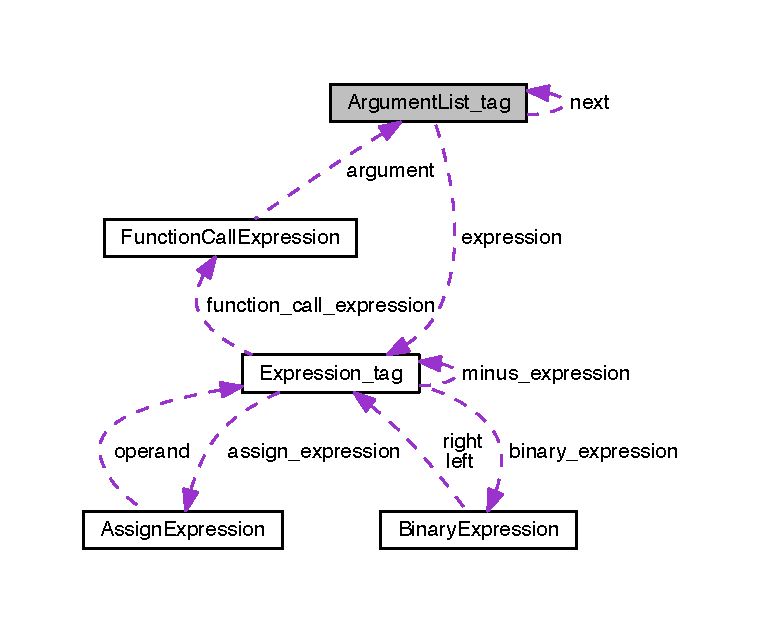
\includegraphics[width=350pt]{struct_argument_list__tag__coll__graph}
\end{center}
\end{figure}
\subsection*{Public Attributes}
\begin{DoxyCompactItemize}
\item 
\hyperlink{crowbar_8h_a070c6feb370aad8a9665ca315bf6ed4a}{Expression} $\ast$ \hyperlink{struct_argument_list__tag_a90b0642f2ea0053d4382053fe4fb397b}{expression}
\item 
struct \hyperlink{struct_argument_list__tag}{Argument\+List\+\_\+tag} $\ast$ \hyperlink{struct_argument_list__tag_adf51711dee3b1c443d0f75a92c0a8d6b}{next}
\end{DoxyCompactItemize}


\subsection{Member Data Documentation}
\hypertarget{struct_argument_list__tag_a90b0642f2ea0053d4382053fe4fb397b}{}\index{Argument\+List\+\_\+tag@{Argument\+List\+\_\+tag}!expression@{expression}}
\index{expression@{expression}!Argument\+List\+\_\+tag@{Argument\+List\+\_\+tag}}
\subsubsection[{expression}]{\setlength{\rightskip}{0pt plus 5cm}{\bf Expression}$\ast$ Argument\+List\+\_\+tag\+::expression}\label{struct_argument_list__tag_a90b0642f2ea0053d4382053fe4fb397b}
\hypertarget{struct_argument_list__tag_adf51711dee3b1c443d0f75a92c0a8d6b}{}\index{Argument\+List\+\_\+tag@{Argument\+List\+\_\+tag}!next@{next}}
\index{next@{next}!Argument\+List\+\_\+tag@{Argument\+List\+\_\+tag}}
\subsubsection[{next}]{\setlength{\rightskip}{0pt plus 5cm}struct {\bf Argument\+List\+\_\+tag}$\ast$ Argument\+List\+\_\+tag\+::next}\label{struct_argument_list__tag_adf51711dee3b1c443d0f75a92c0a8d6b}


The documentation for this struct was generated from the following file\+:\begin{DoxyCompactItemize}
\item 
\hyperlink{crowbar_8h}{crowbar.\+h}\end{DoxyCompactItemize}

\hypertarget{struct_assign_expression}{}\section{Assign\+Expression Struct Reference}
\label{struct_assign_expression}\index{Assign\+Expression@{Assign\+Expression}}


{\ttfamily \#include $<$crowbar.\+h$>$}



Collaboration diagram for Assign\+Expression\+:\nopagebreak
\begin{figure}[H]
\begin{center}
\leavevmode
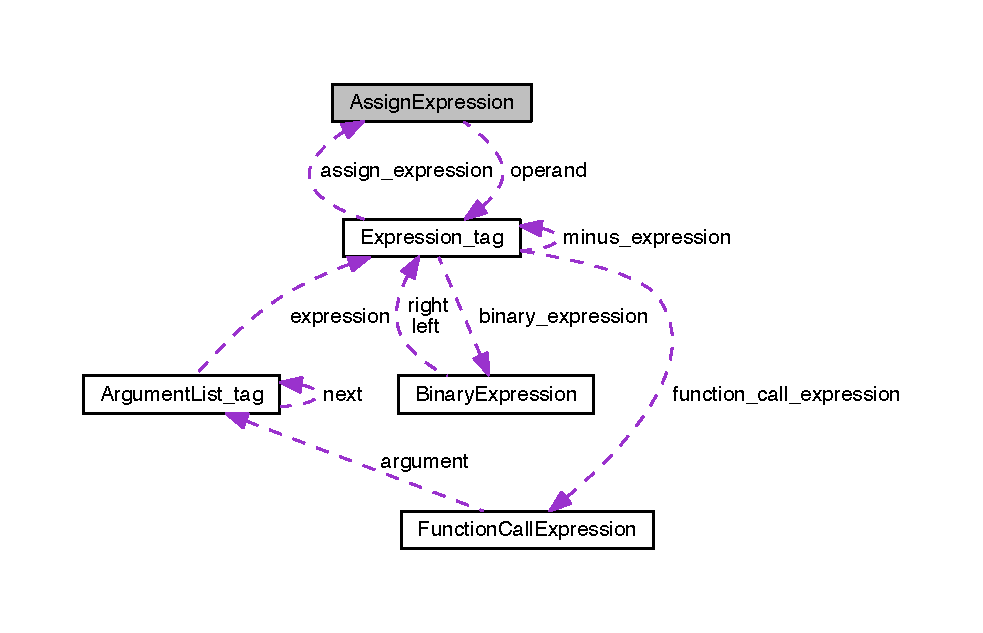
\includegraphics[width=350pt]{struct_assign_expression__coll__graph}
\end{center}
\end{figure}
\subsection*{Public Attributes}
\begin{DoxyCompactItemize}
\item 
char $\ast$ \hyperlink{struct_assign_expression_a0f54a893d9f786a38c10c166caa7dd08}{variable}
\item 
\hyperlink{crowbar_8h_a070c6feb370aad8a9665ca315bf6ed4a}{Expression} $\ast$ \hyperlink{struct_assign_expression_ae2bc8d22ef9baa0b02a484c3284559a6}{operand}
\end{DoxyCompactItemize}


\subsection{Member Data Documentation}
\hypertarget{struct_assign_expression_ae2bc8d22ef9baa0b02a484c3284559a6}{}\index{Assign\+Expression@{Assign\+Expression}!operand@{operand}}
\index{operand@{operand}!Assign\+Expression@{Assign\+Expression}}
\subsubsection[{operand}]{\setlength{\rightskip}{0pt plus 5cm}{\bf Expression}$\ast$ Assign\+Expression\+::operand}\label{struct_assign_expression_ae2bc8d22ef9baa0b02a484c3284559a6}
\hypertarget{struct_assign_expression_a0f54a893d9f786a38c10c166caa7dd08}{}\index{Assign\+Expression@{Assign\+Expression}!variable@{variable}}
\index{variable@{variable}!Assign\+Expression@{Assign\+Expression}}
\subsubsection[{variable}]{\setlength{\rightskip}{0pt plus 5cm}char$\ast$ Assign\+Expression\+::variable}\label{struct_assign_expression_a0f54a893d9f786a38c10c166caa7dd08}


The documentation for this struct was generated from the following file\+:\begin{DoxyCompactItemize}
\item 
\hyperlink{crowbar_8h}{crowbar.\+h}\end{DoxyCompactItemize}

\hypertarget{struct_binary_expression}{}\section{Binary\+Expression Struct Reference}
\label{struct_binary_expression}\index{Binary\+Expression@{Binary\+Expression}}


{\ttfamily \#include $<$crowbar.\+h$>$}



Collaboration diagram for Binary\+Expression\+:\nopagebreak
\begin{figure}[H]
\begin{center}
\leavevmode
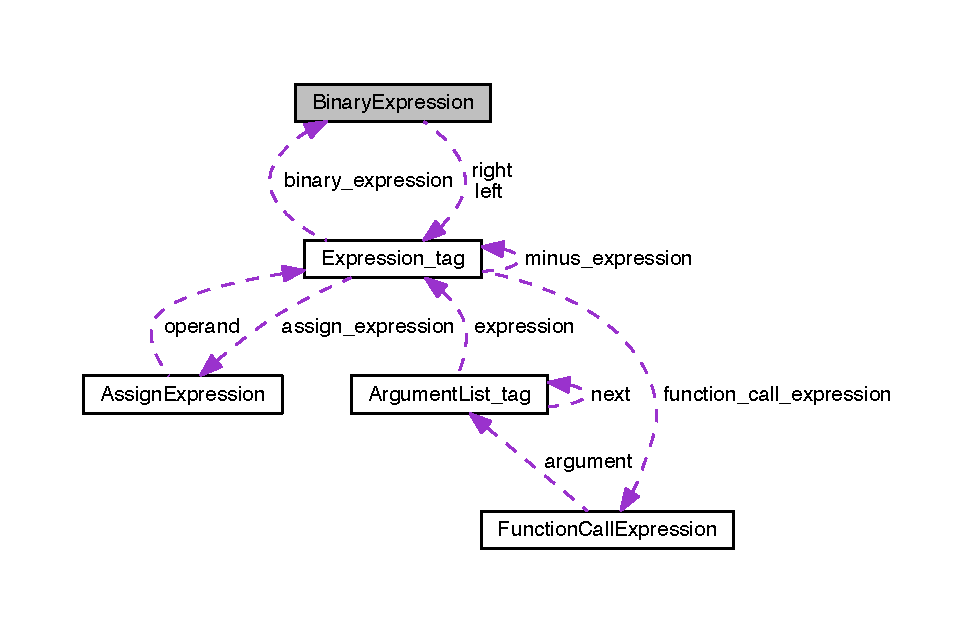
\includegraphics[width=350pt]{struct_binary_expression__coll__graph}
\end{center}
\end{figure}
\subsection*{Public Attributes}
\begin{DoxyCompactItemize}
\item 
\hyperlink{crowbar_8h_a070c6feb370aad8a9665ca315bf6ed4a}{Expression} $\ast$ \hyperlink{struct_binary_expression_aa9afb47a0f44456caa7094ff4de7e2e3}{left}
\item 
\hyperlink{crowbar_8h_a070c6feb370aad8a9665ca315bf6ed4a}{Expression} $\ast$ \hyperlink{struct_binary_expression_a22065ee718926701c8f1d70080b61636}{right}
\end{DoxyCompactItemize}


\subsection{Member Data Documentation}
\hypertarget{struct_binary_expression_aa9afb47a0f44456caa7094ff4de7e2e3}{}\index{Binary\+Expression@{Binary\+Expression}!left@{left}}
\index{left@{left}!Binary\+Expression@{Binary\+Expression}}
\subsubsection[{left}]{\setlength{\rightskip}{0pt plus 5cm}{\bf Expression}$\ast$ Binary\+Expression\+::left}\label{struct_binary_expression_aa9afb47a0f44456caa7094ff4de7e2e3}
\hypertarget{struct_binary_expression_a22065ee718926701c8f1d70080b61636}{}\index{Binary\+Expression@{Binary\+Expression}!right@{right}}
\index{right@{right}!Binary\+Expression@{Binary\+Expression}}
\subsubsection[{right}]{\setlength{\rightskip}{0pt plus 5cm}{\bf Expression}$\ast$ Binary\+Expression\+::right}\label{struct_binary_expression_a22065ee718926701c8f1d70080b61636}


The documentation for this struct was generated from the following file\+:\begin{DoxyCompactItemize}
\item 
\hyperlink{crowbar_8h}{crowbar.\+h}\end{DoxyCompactItemize}

\hypertarget{struct_block}{}\section{Block Struct Reference}
\label{struct_block}\index{Block@{Block}}


{\ttfamily \#include $<$crowbar.\+h$>$}



Collaboration diagram for Block\+:\nopagebreak
\begin{figure}[H]
\begin{center}
\leavevmode
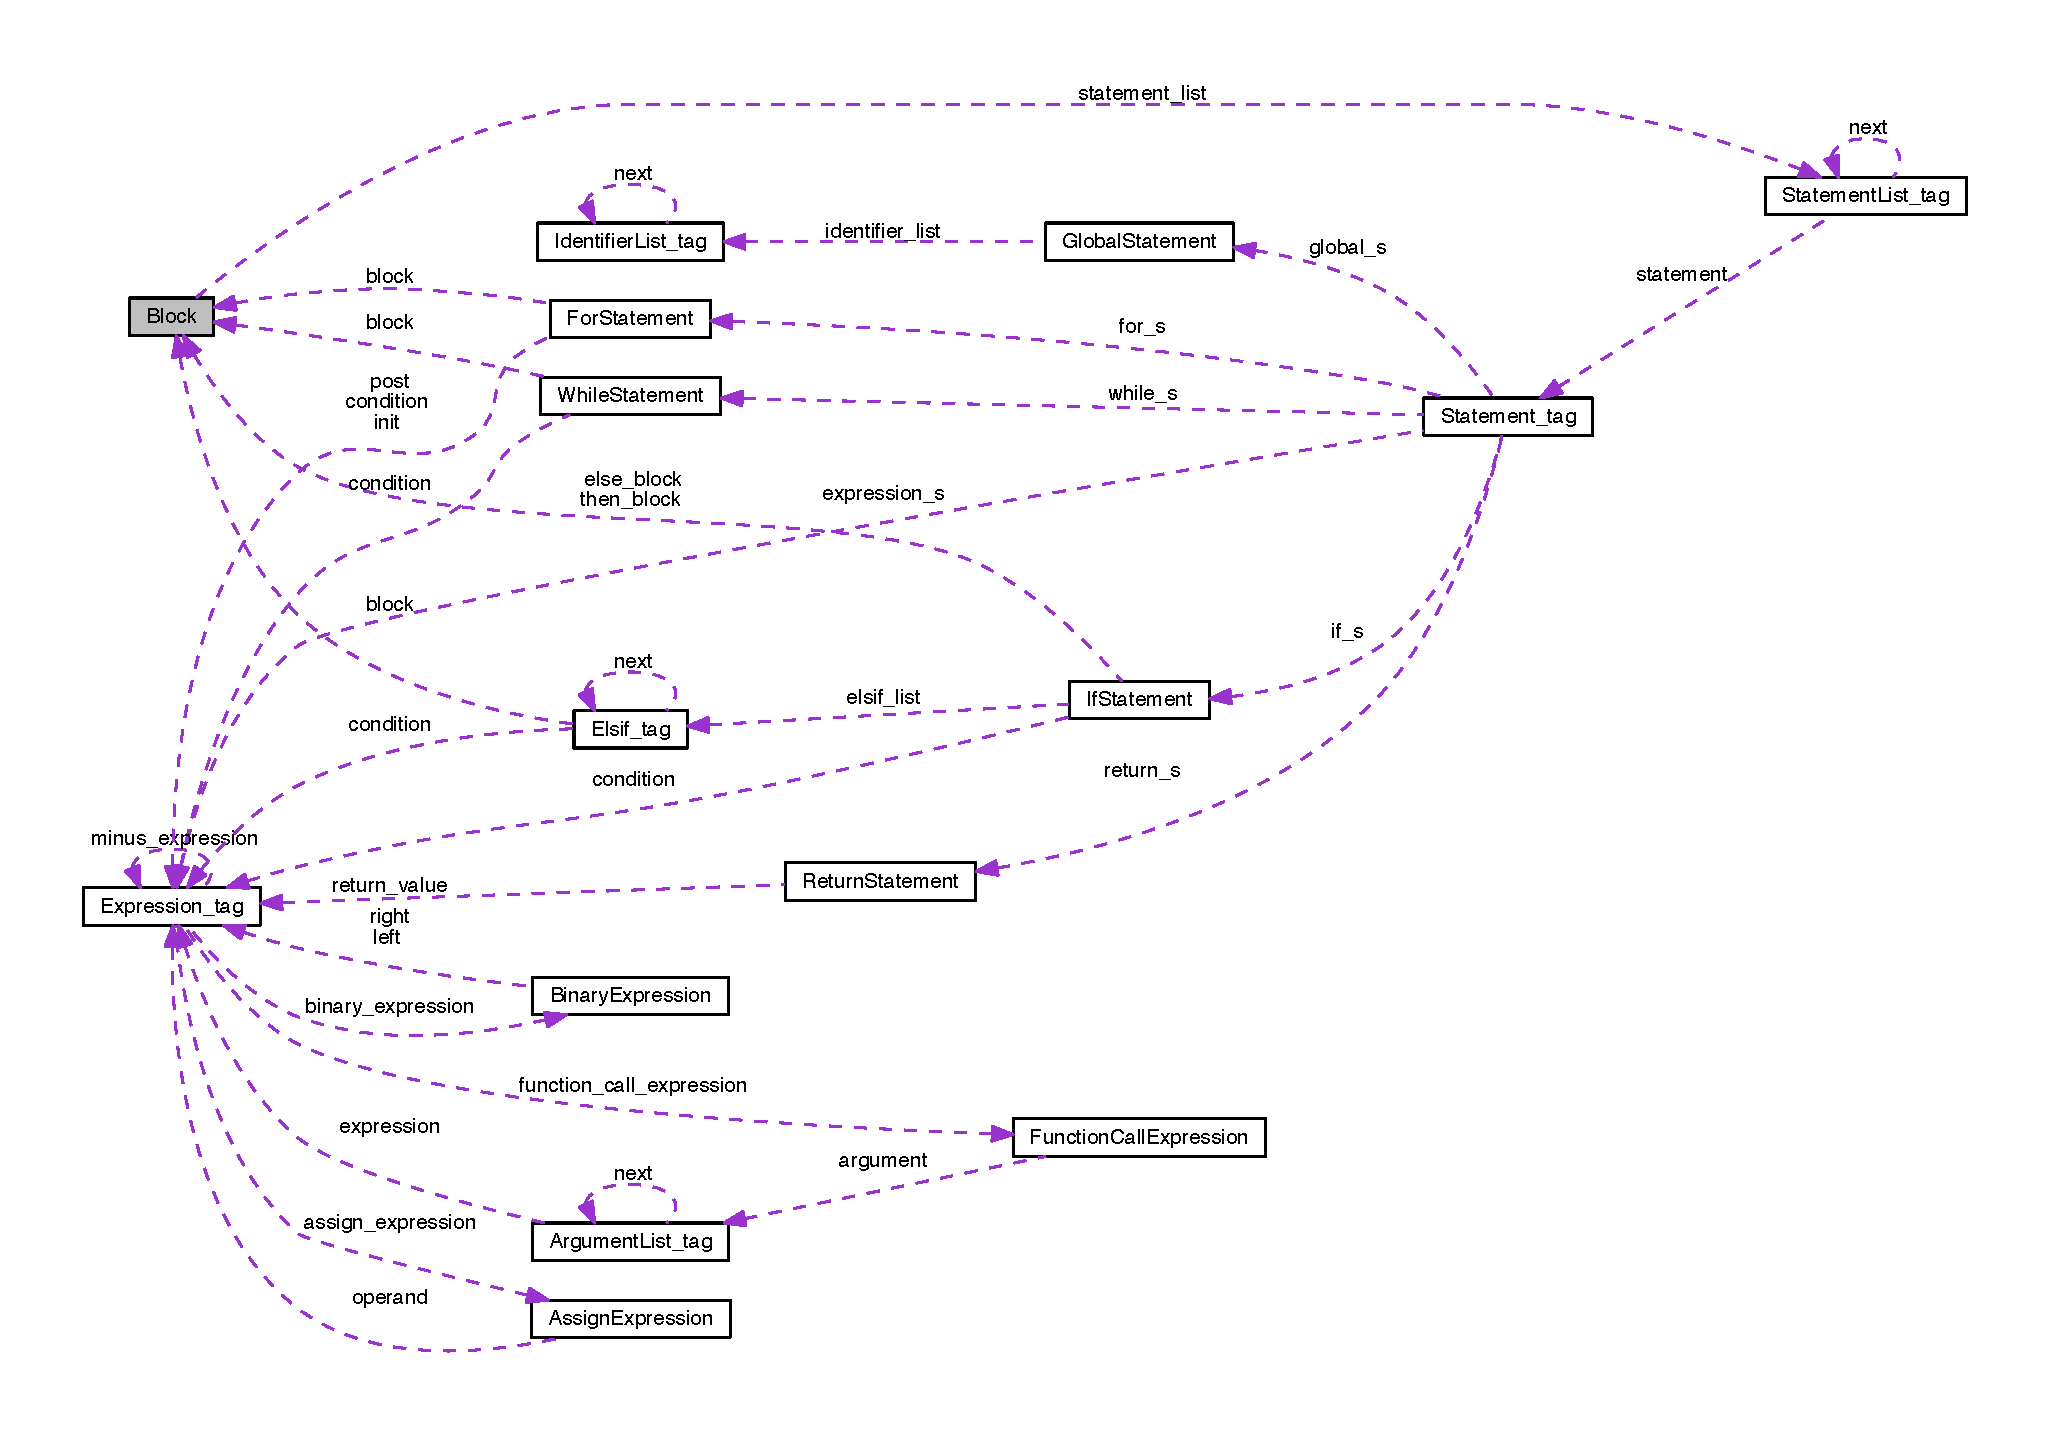
\includegraphics[width=350pt]{struct_block__coll__graph}
\end{center}
\end{figure}
\subsection*{Public Attributes}
\begin{DoxyCompactItemize}
\item 
\hyperlink{crowbar_8h_a8bffae51ec8146f480c3c14c61b4ff93}{Statement\+List} $\ast$ \hyperlink{struct_block_a1f7e56d13e2d1c72dce500d10253bc25}{statement\+\_\+list}
\end{DoxyCompactItemize}


\subsection{Member Data Documentation}
\hypertarget{struct_block_a1f7e56d13e2d1c72dce500d10253bc25}{}\index{Block@{Block}!statement\+\_\+list@{statement\+\_\+list}}
\index{statement\+\_\+list@{statement\+\_\+list}!Block@{Block}}
\subsubsection[{statement\+\_\+list}]{\setlength{\rightskip}{0pt plus 5cm}{\bf Statement\+List}$\ast$ Block\+::statement\+\_\+list}\label{struct_block_a1f7e56d13e2d1c72dce500d10253bc25}


The documentation for this struct was generated from the following file\+:\begin{DoxyCompactItemize}
\item 
\hyperlink{crowbar_8h}{crowbar.\+h}\end{DoxyCompactItemize}

\hypertarget{union_cell}{}\section{Cell Union Reference}
\label{union_cell}\index{Cell@{Cell}}
\subsection*{Public Attributes}
\begin{DoxyCompactItemize}
\item 
long \hyperlink{union_cell_a1a43c4a13dabb18afb6cc6abab3c5dd3}{l\+\_\+dummy}
\item 
double \hyperlink{union_cell_a00a7dcdf70d80970444665f97eeddfbe}{d\+\_\+dummy}
\item 
void $\ast$ \hyperlink{union_cell_a690f8a25336f573548b07ae33d008fde}{p\+\_\+dummy}
\end{DoxyCompactItemize}


\subsection{Member Data Documentation}
\hypertarget{union_cell_a00a7dcdf70d80970444665f97eeddfbe}{}\index{Cell@{Cell}!d\+\_\+dummy@{d\+\_\+dummy}}
\index{d\+\_\+dummy@{d\+\_\+dummy}!Cell@{Cell}}
\subsubsection[{d\+\_\+dummy}]{\setlength{\rightskip}{0pt plus 5cm}double Cell\+::d\+\_\+dummy}\label{union_cell_a00a7dcdf70d80970444665f97eeddfbe}
\hypertarget{union_cell_a1a43c4a13dabb18afb6cc6abab3c5dd3}{}\index{Cell@{Cell}!l\+\_\+dummy@{l\+\_\+dummy}}
\index{l\+\_\+dummy@{l\+\_\+dummy}!Cell@{Cell}}
\subsubsection[{l\+\_\+dummy}]{\setlength{\rightskip}{0pt plus 5cm}long Cell\+::l\+\_\+dummy}\label{union_cell_a1a43c4a13dabb18afb6cc6abab3c5dd3}
\hypertarget{union_cell_a690f8a25336f573548b07ae33d008fde}{}\index{Cell@{Cell}!p\+\_\+dummy@{p\+\_\+dummy}}
\index{p\+\_\+dummy@{p\+\_\+dummy}!Cell@{Cell}}
\subsubsection[{p\+\_\+dummy}]{\setlength{\rightskip}{0pt plus 5cm}void$\ast$ Cell\+::p\+\_\+dummy}\label{union_cell_a690f8a25336f573548b07ae33d008fde}


The documentation for this union was generated from the following file\+:\begin{DoxyCompactItemize}
\item 
memory/\hyperlink{storage_8c}{storage.\+c}\end{DoxyCompactItemize}

\hypertarget{struct_c_r_b___interpreter__tag}{}\section{C\+R\+B\+\_\+\+Interpreter\+\_\+tag Struct Reference}
\label{struct_c_r_b___interpreter__tag}\index{C\+R\+B\+\_\+\+Interpreter\+\_\+tag@{C\+R\+B\+\_\+\+Interpreter\+\_\+tag}}


{\ttfamily \#include $<$crowbar.\+h$>$}



Collaboration diagram for C\+R\+B\+\_\+\+Interpreter\+\_\+tag\+:\nopagebreak
\begin{figure}[H]
\begin{center}
\leavevmode
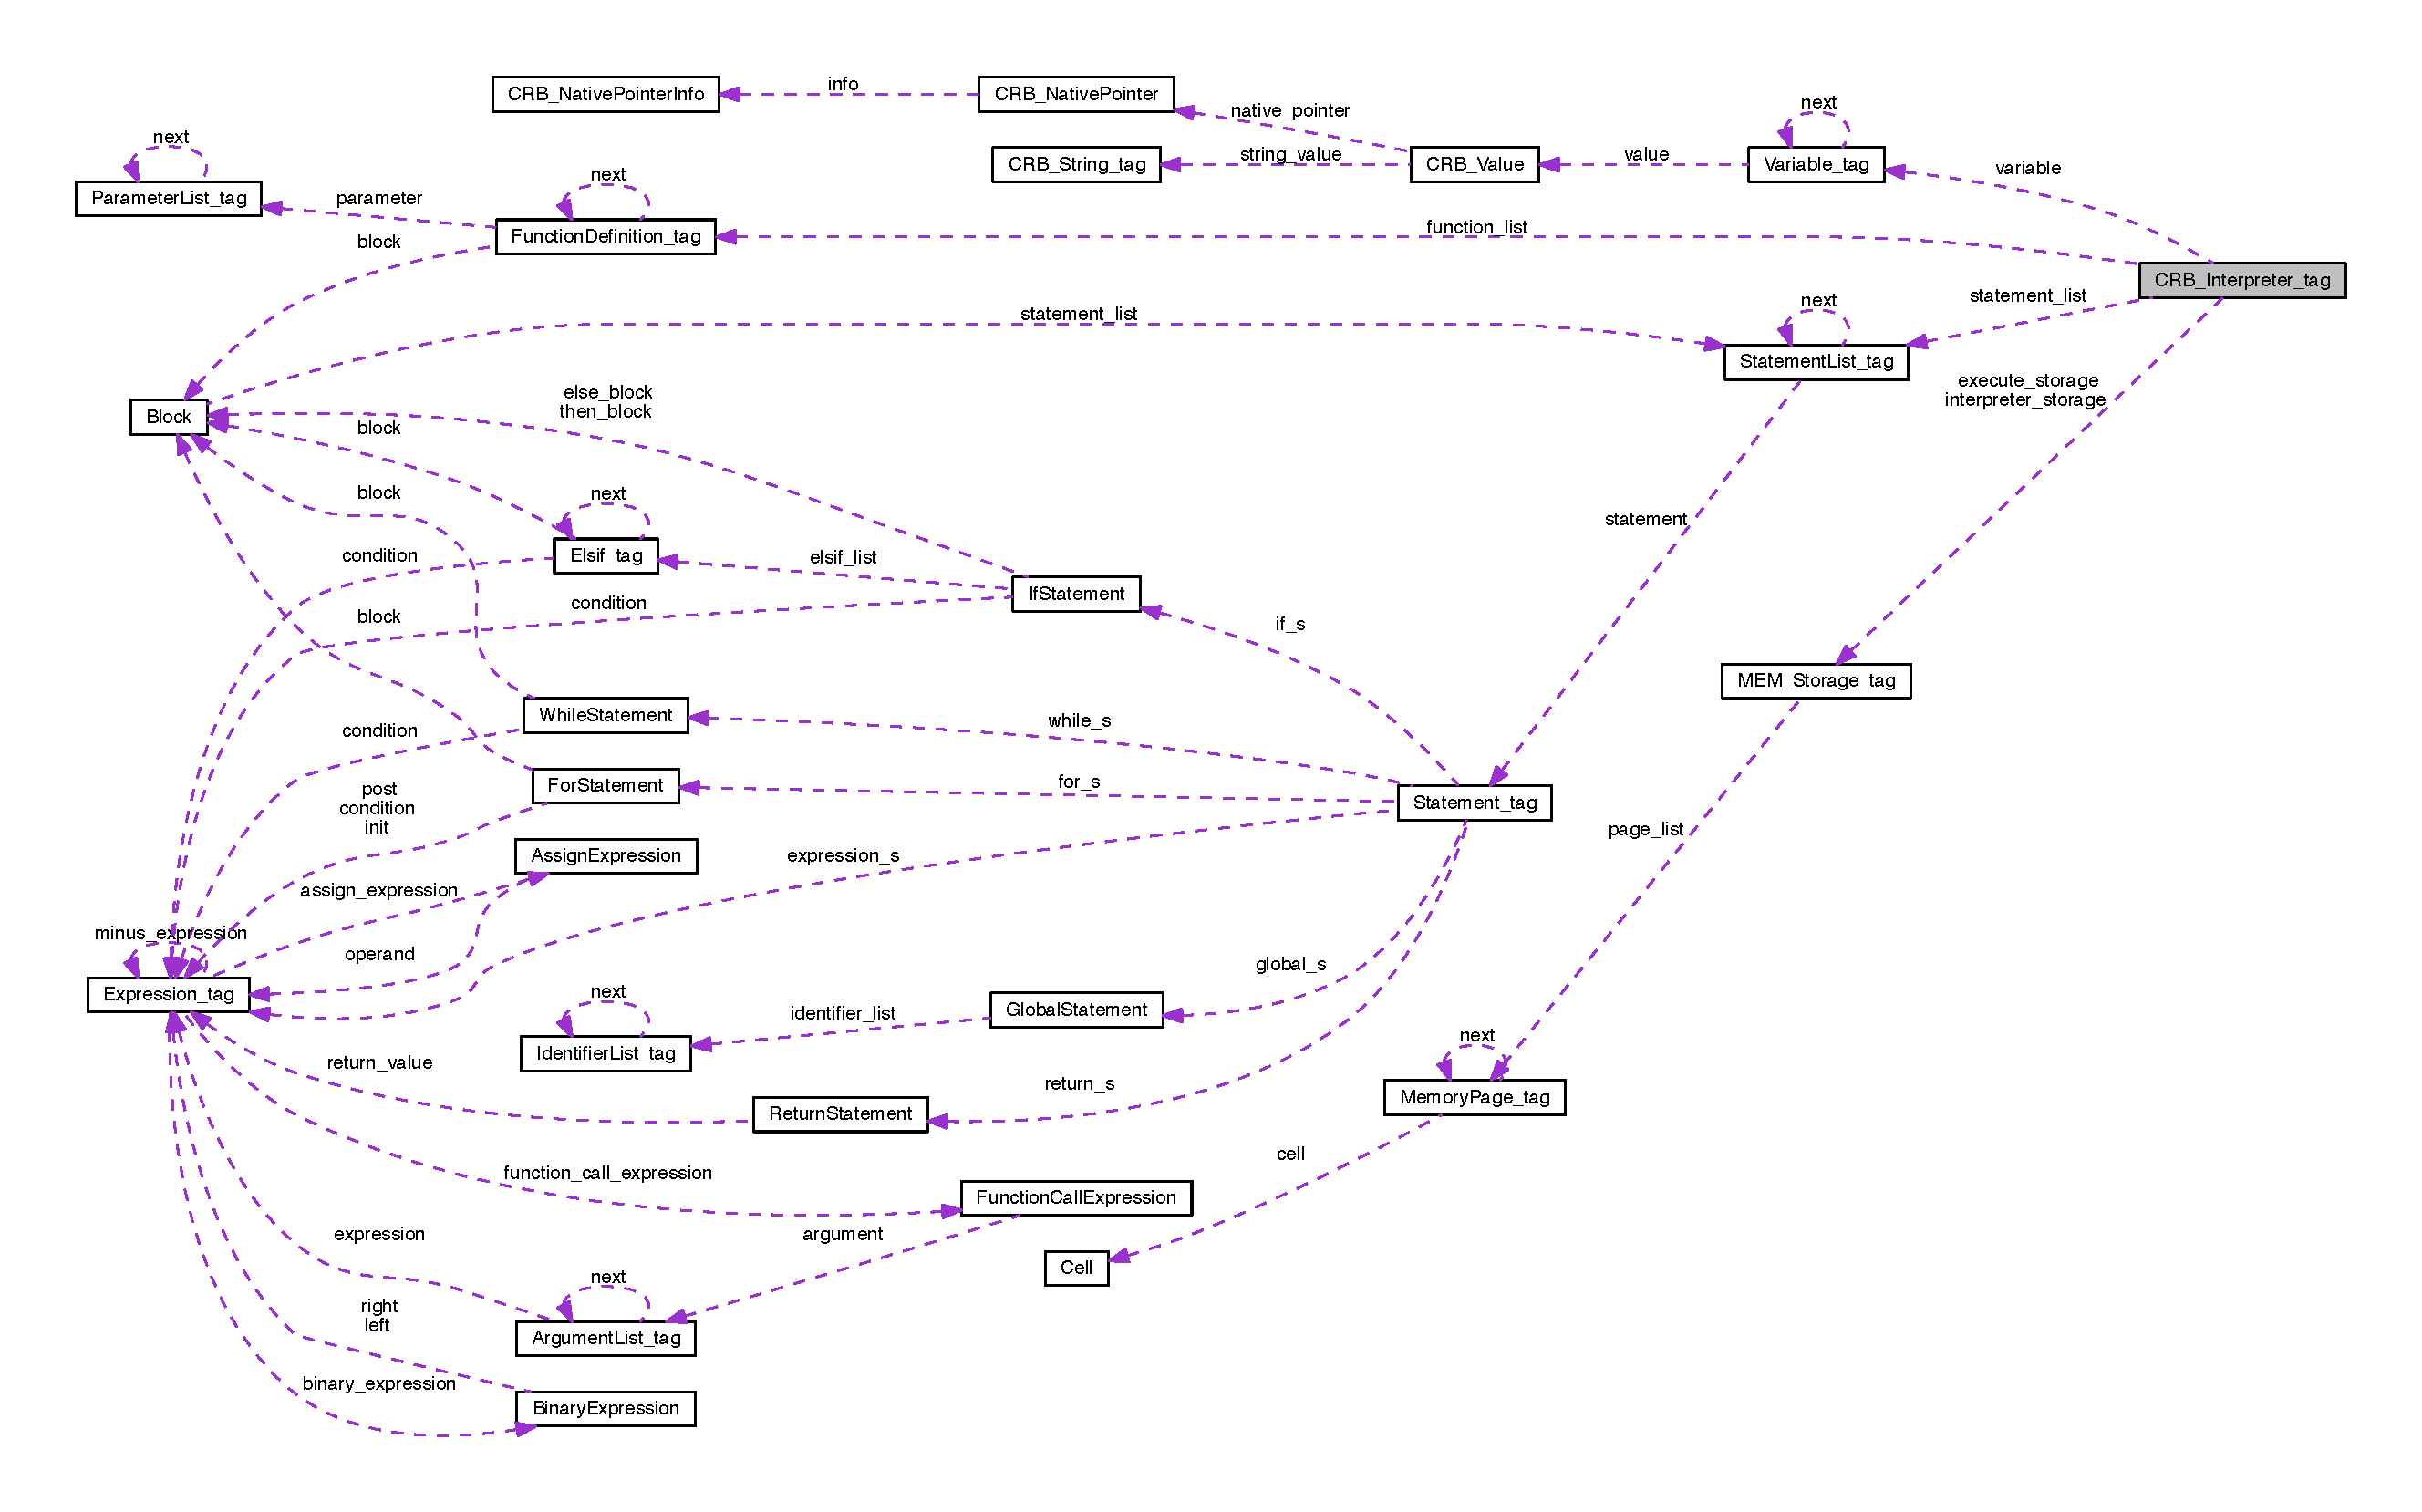
\includegraphics[width=350pt]{struct_c_r_b___interpreter__tag__coll__graph}
\end{center}
\end{figure}
\subsection*{Public Attributes}
\begin{DoxyCompactItemize}
\item 
\hyperlink{_m_e_m_8h_afc904fd630ab1c716f8e0a1096f62697}{M\+E\+M\+\_\+\+Storage} \hyperlink{struct_c_r_b___interpreter__tag_a6959871398b2d3b1711e9f80a3e2dd4e}{interpreter\+\_\+storage}
\item 
\hyperlink{_m_e_m_8h_afc904fd630ab1c716f8e0a1096f62697}{M\+E\+M\+\_\+\+Storage} \hyperlink{struct_c_r_b___interpreter__tag_acbd5f1ff1ab29110408a2e41a98196d0}{execute\+\_\+storage}
\item 
\hyperlink{crowbar_8h_a070c86ad7ae39536aed471927d04dee4}{Variable} $\ast$ \hyperlink{struct_c_r_b___interpreter__tag_a9226949153a3c16dbd27830598997930}{variable}
\item 
\hyperlink{crowbar_8h_ae6685df239452173440b6042201dbd9f}{Function\+Definition} $\ast$ \hyperlink{struct_c_r_b___interpreter__tag_aea5177d1aa33b19f82430f097f95b15b}{function\+\_\+list}
\item 
\hyperlink{crowbar_8h_a8bffae51ec8146f480c3c14c61b4ff93}{Statement\+List} $\ast$ \hyperlink{struct_c_r_b___interpreter__tag_a8d794cdb4f087bf09998f1979062b4f6}{statement\+\_\+list}
\item 
int \hyperlink{struct_c_r_b___interpreter__tag_a0e7113d528b4c75dd34ece37eacbfdfd}{current\+\_\+line\+\_\+number}
\end{DoxyCompactItemize}


\subsection{Member Data Documentation}
\hypertarget{struct_c_r_b___interpreter__tag_a0e7113d528b4c75dd34ece37eacbfdfd}{}\index{C\+R\+B\+\_\+\+Interpreter\+\_\+tag@{C\+R\+B\+\_\+\+Interpreter\+\_\+tag}!current\+\_\+line\+\_\+number@{current\+\_\+line\+\_\+number}}
\index{current\+\_\+line\+\_\+number@{current\+\_\+line\+\_\+number}!C\+R\+B\+\_\+\+Interpreter\+\_\+tag@{C\+R\+B\+\_\+\+Interpreter\+\_\+tag}}
\subsubsection[{current\+\_\+line\+\_\+number}]{\setlength{\rightskip}{0pt plus 5cm}int C\+R\+B\+\_\+\+Interpreter\+\_\+tag\+::current\+\_\+line\+\_\+number}\label{struct_c_r_b___interpreter__tag_a0e7113d528b4c75dd34ece37eacbfdfd}
\hypertarget{struct_c_r_b___interpreter__tag_acbd5f1ff1ab29110408a2e41a98196d0}{}\index{C\+R\+B\+\_\+\+Interpreter\+\_\+tag@{C\+R\+B\+\_\+\+Interpreter\+\_\+tag}!execute\+\_\+storage@{execute\+\_\+storage}}
\index{execute\+\_\+storage@{execute\+\_\+storage}!C\+R\+B\+\_\+\+Interpreter\+\_\+tag@{C\+R\+B\+\_\+\+Interpreter\+\_\+tag}}
\subsubsection[{execute\+\_\+storage}]{\setlength{\rightskip}{0pt plus 5cm}{\bf M\+E\+M\+\_\+\+Storage} C\+R\+B\+\_\+\+Interpreter\+\_\+tag\+::execute\+\_\+storage}\label{struct_c_r_b___interpreter__tag_acbd5f1ff1ab29110408a2e41a98196d0}
\hypertarget{struct_c_r_b___interpreter__tag_aea5177d1aa33b19f82430f097f95b15b}{}\index{C\+R\+B\+\_\+\+Interpreter\+\_\+tag@{C\+R\+B\+\_\+\+Interpreter\+\_\+tag}!function\+\_\+list@{function\+\_\+list}}
\index{function\+\_\+list@{function\+\_\+list}!C\+R\+B\+\_\+\+Interpreter\+\_\+tag@{C\+R\+B\+\_\+\+Interpreter\+\_\+tag}}
\subsubsection[{function\+\_\+list}]{\setlength{\rightskip}{0pt plus 5cm}{\bf Function\+Definition}$\ast$ C\+R\+B\+\_\+\+Interpreter\+\_\+tag\+::function\+\_\+list}\label{struct_c_r_b___interpreter__tag_aea5177d1aa33b19f82430f097f95b15b}
\hypertarget{struct_c_r_b___interpreter__tag_a6959871398b2d3b1711e9f80a3e2dd4e}{}\index{C\+R\+B\+\_\+\+Interpreter\+\_\+tag@{C\+R\+B\+\_\+\+Interpreter\+\_\+tag}!interpreter\+\_\+storage@{interpreter\+\_\+storage}}
\index{interpreter\+\_\+storage@{interpreter\+\_\+storage}!C\+R\+B\+\_\+\+Interpreter\+\_\+tag@{C\+R\+B\+\_\+\+Interpreter\+\_\+tag}}
\subsubsection[{interpreter\+\_\+storage}]{\setlength{\rightskip}{0pt plus 5cm}{\bf M\+E\+M\+\_\+\+Storage} C\+R\+B\+\_\+\+Interpreter\+\_\+tag\+::interpreter\+\_\+storage}\label{struct_c_r_b___interpreter__tag_a6959871398b2d3b1711e9f80a3e2dd4e}
\hypertarget{struct_c_r_b___interpreter__tag_a8d794cdb4f087bf09998f1979062b4f6}{}\index{C\+R\+B\+\_\+\+Interpreter\+\_\+tag@{C\+R\+B\+\_\+\+Interpreter\+\_\+tag}!statement\+\_\+list@{statement\+\_\+list}}
\index{statement\+\_\+list@{statement\+\_\+list}!C\+R\+B\+\_\+\+Interpreter\+\_\+tag@{C\+R\+B\+\_\+\+Interpreter\+\_\+tag}}
\subsubsection[{statement\+\_\+list}]{\setlength{\rightskip}{0pt plus 5cm}{\bf Statement\+List}$\ast$ C\+R\+B\+\_\+\+Interpreter\+\_\+tag\+::statement\+\_\+list}\label{struct_c_r_b___interpreter__tag_a8d794cdb4f087bf09998f1979062b4f6}
\hypertarget{struct_c_r_b___interpreter__tag_a9226949153a3c16dbd27830598997930}{}\index{C\+R\+B\+\_\+\+Interpreter\+\_\+tag@{C\+R\+B\+\_\+\+Interpreter\+\_\+tag}!variable@{variable}}
\index{variable@{variable}!C\+R\+B\+\_\+\+Interpreter\+\_\+tag@{C\+R\+B\+\_\+\+Interpreter\+\_\+tag}}
\subsubsection[{variable}]{\setlength{\rightskip}{0pt plus 5cm}{\bf Variable}$\ast$ C\+R\+B\+\_\+\+Interpreter\+\_\+tag\+::variable}\label{struct_c_r_b___interpreter__tag_a9226949153a3c16dbd27830598997930}


The documentation for this struct was generated from the following file\+:\begin{DoxyCompactItemize}
\item 
\hyperlink{crowbar_8h}{crowbar.\+h}\end{DoxyCompactItemize}

\hypertarget{struct_c_r_b___native_pointer}{}\section{C\+R\+B\+\_\+\+Native\+Pointer Struct Reference}
\label{struct_c_r_b___native_pointer}\index{C\+R\+B\+\_\+\+Native\+Pointer@{C\+R\+B\+\_\+\+Native\+Pointer}}


{\ttfamily \#include $<$C\+R\+B\+\_\+dev.\+h$>$}



Collaboration diagram for C\+R\+B\+\_\+\+Native\+Pointer\+:\nopagebreak
\begin{figure}[H]
\begin{center}
\leavevmode
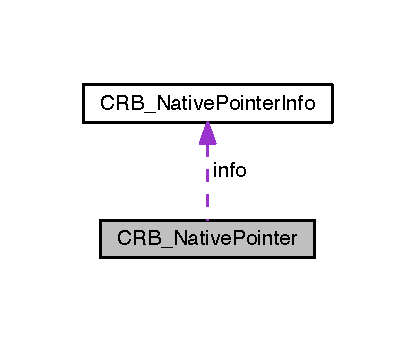
\includegraphics[width=199pt]{struct_c_r_b___native_pointer__coll__graph}
\end{center}
\end{figure}
\subsection*{Public Attributes}
\begin{DoxyCompactItemize}
\item 
\hyperlink{struct_c_r_b___native_pointer_info}{C\+R\+B\+\_\+\+Native\+Pointer\+Info} $\ast$ \hyperlink{struct_c_r_b___native_pointer_af2aec2f2878e463a14f8c203f48a372e}{info}
\item 
void $\ast$ \hyperlink{struct_c_r_b___native_pointer_ad4bda48ee3efc0fc0c7b1a3bd6409903}{pointer}
\end{DoxyCompactItemize}


\subsection{Member Data Documentation}
\hypertarget{struct_c_r_b___native_pointer_af2aec2f2878e463a14f8c203f48a372e}{}\index{C\+R\+B\+\_\+\+Native\+Pointer@{C\+R\+B\+\_\+\+Native\+Pointer}!info@{info}}
\index{info@{info}!C\+R\+B\+\_\+\+Native\+Pointer@{C\+R\+B\+\_\+\+Native\+Pointer}}
\subsubsection[{info}]{\setlength{\rightskip}{0pt plus 5cm}{\bf C\+R\+B\+\_\+\+Native\+Pointer\+Info}$\ast$ C\+R\+B\+\_\+\+Native\+Pointer\+::info}\label{struct_c_r_b___native_pointer_af2aec2f2878e463a14f8c203f48a372e}
\hypertarget{struct_c_r_b___native_pointer_ad4bda48ee3efc0fc0c7b1a3bd6409903}{}\index{C\+R\+B\+\_\+\+Native\+Pointer@{C\+R\+B\+\_\+\+Native\+Pointer}!pointer@{pointer}}
\index{pointer@{pointer}!C\+R\+B\+\_\+\+Native\+Pointer@{C\+R\+B\+\_\+\+Native\+Pointer}}
\subsubsection[{pointer}]{\setlength{\rightskip}{0pt plus 5cm}void$\ast$ C\+R\+B\+\_\+\+Native\+Pointer\+::pointer}\label{struct_c_r_b___native_pointer_ad4bda48ee3efc0fc0c7b1a3bd6409903}


The documentation for this struct was generated from the following file\+:\begin{DoxyCompactItemize}
\item 
\hyperlink{_c_r_b__dev_8h}{C\+R\+B\+\_\+dev.\+h}\end{DoxyCompactItemize}

\hypertarget{struct_c_r_b___native_pointer_info}{}\section{C\+R\+B\+\_\+\+Native\+Pointer\+Info Struct Reference}
\label{struct_c_r_b___native_pointer_info}\index{C\+R\+B\+\_\+\+Native\+Pointer\+Info@{C\+R\+B\+\_\+\+Native\+Pointer\+Info}}


{\ttfamily \#include $<$C\+R\+B\+\_\+dev.\+h$>$}

\subsection*{Public Attributes}
\begin{DoxyCompactItemize}
\item 
char $\ast$ \hyperlink{struct_c_r_b___native_pointer_info_a5bd97f52968a21784a12a79995834703}{name}
\end{DoxyCompactItemize}


\subsection{Member Data Documentation}
\hypertarget{struct_c_r_b___native_pointer_info_a5bd97f52968a21784a12a79995834703}{}\index{C\+R\+B\+\_\+\+Native\+Pointer\+Info@{C\+R\+B\+\_\+\+Native\+Pointer\+Info}!name@{name}}
\index{name@{name}!C\+R\+B\+\_\+\+Native\+Pointer\+Info@{C\+R\+B\+\_\+\+Native\+Pointer\+Info}}
\subsubsection[{name}]{\setlength{\rightskip}{0pt plus 5cm}char$\ast$ C\+R\+B\+\_\+\+Native\+Pointer\+Info\+::name}\label{struct_c_r_b___native_pointer_info_a5bd97f52968a21784a12a79995834703}


The documentation for this struct was generated from the following file\+:\begin{DoxyCompactItemize}
\item 
\hyperlink{_c_r_b__dev_8h}{C\+R\+B\+\_\+dev.\+h}\end{DoxyCompactItemize}

\hypertarget{struct_c_r_b___string__tag}{}\section{C\+R\+B\+\_\+\+String\+\_\+tag Struct Reference}
\label{struct_c_r_b___string__tag}\index{C\+R\+B\+\_\+\+String\+\_\+tag@{C\+R\+B\+\_\+\+String\+\_\+tag}}


{\ttfamily \#include $<$crowbar.\+h$>$}

\subsection*{Public Attributes}
\begin{DoxyCompactItemize}
\item 
int \hyperlink{struct_c_r_b___string__tag_ace00533a7fe483a5f939f0fd59903dd7}{ref\+\_\+count}
\item 
char $\ast$ \hyperlink{struct_c_r_b___string__tag_a797e7b2d75e0c612d1a1a956d2ffd5ad}{string}
\item 
\hyperlink{_c_r_b__dev_8h_a5000f2b447c9132c07d7f1cf66134a69}{C\+R\+B\+\_\+\+Boolean} \hyperlink{struct_c_r_b___string__tag_a82d515771ee47a64edd80c656f9eadc5}{is\+\_\+literal}
\end{DoxyCompactItemize}


\subsection{Member Data Documentation}
\hypertarget{struct_c_r_b___string__tag_a82d515771ee47a64edd80c656f9eadc5}{}\index{C\+R\+B\+\_\+\+String\+\_\+tag@{C\+R\+B\+\_\+\+String\+\_\+tag}!is\+\_\+literal@{is\+\_\+literal}}
\index{is\+\_\+literal@{is\+\_\+literal}!C\+R\+B\+\_\+\+String\+\_\+tag@{C\+R\+B\+\_\+\+String\+\_\+tag}}
\subsubsection[{is\+\_\+literal}]{\setlength{\rightskip}{0pt plus 5cm}{\bf C\+R\+B\+\_\+\+Boolean} C\+R\+B\+\_\+\+String\+\_\+tag\+::is\+\_\+literal}\label{struct_c_r_b___string__tag_a82d515771ee47a64edd80c656f9eadc5}
\hypertarget{struct_c_r_b___string__tag_ace00533a7fe483a5f939f0fd59903dd7}{}\index{C\+R\+B\+\_\+\+String\+\_\+tag@{C\+R\+B\+\_\+\+String\+\_\+tag}!ref\+\_\+count@{ref\+\_\+count}}
\index{ref\+\_\+count@{ref\+\_\+count}!C\+R\+B\+\_\+\+String\+\_\+tag@{C\+R\+B\+\_\+\+String\+\_\+tag}}
\subsubsection[{ref\+\_\+count}]{\setlength{\rightskip}{0pt plus 5cm}int C\+R\+B\+\_\+\+String\+\_\+tag\+::ref\+\_\+count}\label{struct_c_r_b___string__tag_ace00533a7fe483a5f939f0fd59903dd7}
\hypertarget{struct_c_r_b___string__tag_a797e7b2d75e0c612d1a1a956d2ffd5ad}{}\index{C\+R\+B\+\_\+\+String\+\_\+tag@{C\+R\+B\+\_\+\+String\+\_\+tag}!string@{string}}
\index{string@{string}!C\+R\+B\+\_\+\+String\+\_\+tag@{C\+R\+B\+\_\+\+String\+\_\+tag}}
\subsubsection[{string}]{\setlength{\rightskip}{0pt plus 5cm}char$\ast$ C\+R\+B\+\_\+\+String\+\_\+tag\+::string}\label{struct_c_r_b___string__tag_a797e7b2d75e0c612d1a1a956d2ffd5ad}


The documentation for this struct was generated from the following file\+:\begin{DoxyCompactItemize}
\item 
\hyperlink{crowbar_8h}{crowbar.\+h}\end{DoxyCompactItemize}

\hypertarget{struct_c_r_b___value}{}\section{C\+R\+B\+\_\+\+Value Struct Reference}
\label{struct_c_r_b___value}\index{C\+R\+B\+\_\+\+Value@{C\+R\+B\+\_\+\+Value}}


{\ttfamily \#include $<$C\+R\+B\+\_\+dev.\+h$>$}



Collaboration diagram for C\+R\+B\+\_\+\+Value\+:\nopagebreak
\begin{figure}[H]
\begin{center}
\leavevmode
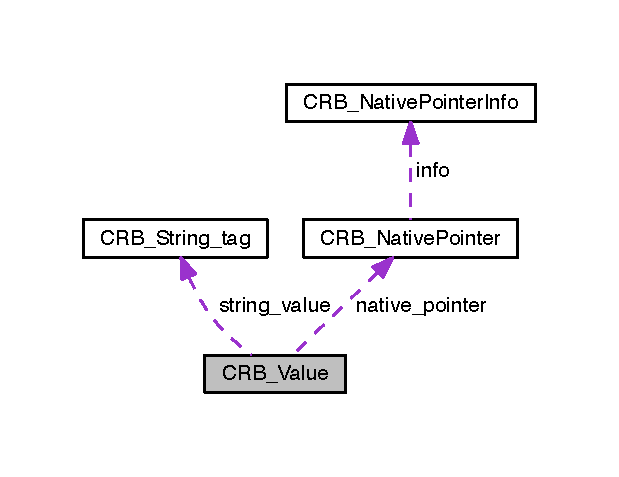
\includegraphics[width=297pt]{struct_c_r_b___value__coll__graph}
\end{center}
\end{figure}
\subsection*{Public Attributes}
\begin{DoxyCompactItemize}
\item 
\hyperlink{_c_r_b__dev_8h_a1a82f38e78e95951e6a9cdc0f5fd4a3a}{C\+R\+B\+\_\+\+Value\+Type} \hyperlink{struct_c_r_b___value_acda650198a166ebbcfdbe3e59c16c48d}{type}
\item 
\begin{tabbing}
xx\=xx\=xx\=xx\=xx\=xx\=xx\=xx\=xx\=\kill
union \{\\
\>\hyperlink{_c_r_b__dev_8h_a5000f2b447c9132c07d7f1cf66134a69}{CRB\_Boolean} \hyperlink{struct_c_r_b___value_ab7a1cd9cc805aa5147dff85998ce9a35}{boolean\_value}\\
\>int \hyperlink{struct_c_r_b___value_af4f8c00699f88b1f66df39533d8a954d}{int\_value}\\
\>double \hyperlink{struct_c_r_b___value_a5d6c2992019285bdf7999e4f577e2a40}{double\_value}\\
\>\hyperlink{_c_r_b__dev_8h_a0372b51b327f3425e983d9924fc713f8}{CRB\_String} $\ast$ \hyperlink{struct_c_r_b___value_abbb38f47b1039d6332e5ccc6e2075ec4}{string\_value}\\
\>\hyperlink{struct_c_r_b___native_pointer}{CRB\_NativePointer} \hyperlink{struct_c_r_b___value_a7aaf59723f27b15f1fcc17bb5dce1edf}{native\_pointer}\\
\} \hyperlink{struct_c_r_b___value_aac6984702013a49c5f0e75e84cfc5bdd}{u}\\

\end{tabbing}\end{DoxyCompactItemize}


\subsection{Member Data Documentation}
\hypertarget{struct_c_r_b___value_ab7a1cd9cc805aa5147dff85998ce9a35}{}\index{C\+R\+B\+\_\+\+Value@{C\+R\+B\+\_\+\+Value}!boolean\+\_\+value@{boolean\+\_\+value}}
\index{boolean\+\_\+value@{boolean\+\_\+value}!C\+R\+B\+\_\+\+Value@{C\+R\+B\+\_\+\+Value}}
\subsubsection[{boolean\+\_\+value}]{\setlength{\rightskip}{0pt plus 5cm}{\bf C\+R\+B\+\_\+\+Boolean} C\+R\+B\+\_\+\+Value\+::boolean\+\_\+value}\label{struct_c_r_b___value_ab7a1cd9cc805aa5147dff85998ce9a35}
\hypertarget{struct_c_r_b___value_a5d6c2992019285bdf7999e4f577e2a40}{}\index{C\+R\+B\+\_\+\+Value@{C\+R\+B\+\_\+\+Value}!double\+\_\+value@{double\+\_\+value}}
\index{double\+\_\+value@{double\+\_\+value}!C\+R\+B\+\_\+\+Value@{C\+R\+B\+\_\+\+Value}}
\subsubsection[{double\+\_\+value}]{\setlength{\rightskip}{0pt plus 5cm}double C\+R\+B\+\_\+\+Value\+::double\+\_\+value}\label{struct_c_r_b___value_a5d6c2992019285bdf7999e4f577e2a40}
\hypertarget{struct_c_r_b___value_af4f8c00699f88b1f66df39533d8a954d}{}\index{C\+R\+B\+\_\+\+Value@{C\+R\+B\+\_\+\+Value}!int\+\_\+value@{int\+\_\+value}}
\index{int\+\_\+value@{int\+\_\+value}!C\+R\+B\+\_\+\+Value@{C\+R\+B\+\_\+\+Value}}
\subsubsection[{int\+\_\+value}]{\setlength{\rightskip}{0pt plus 5cm}int C\+R\+B\+\_\+\+Value\+::int\+\_\+value}\label{struct_c_r_b___value_af4f8c00699f88b1f66df39533d8a954d}
\hypertarget{struct_c_r_b___value_a7aaf59723f27b15f1fcc17bb5dce1edf}{}\index{C\+R\+B\+\_\+\+Value@{C\+R\+B\+\_\+\+Value}!native\+\_\+pointer@{native\+\_\+pointer}}
\index{native\+\_\+pointer@{native\+\_\+pointer}!C\+R\+B\+\_\+\+Value@{C\+R\+B\+\_\+\+Value}}
\subsubsection[{native\+\_\+pointer}]{\setlength{\rightskip}{0pt plus 5cm}{\bf C\+R\+B\+\_\+\+Native\+Pointer} C\+R\+B\+\_\+\+Value\+::native\+\_\+pointer}\label{struct_c_r_b___value_a7aaf59723f27b15f1fcc17bb5dce1edf}
\hypertarget{struct_c_r_b___value_abbb38f47b1039d6332e5ccc6e2075ec4}{}\index{C\+R\+B\+\_\+\+Value@{C\+R\+B\+\_\+\+Value}!string\+\_\+value@{string\+\_\+value}}
\index{string\+\_\+value@{string\+\_\+value}!C\+R\+B\+\_\+\+Value@{C\+R\+B\+\_\+\+Value}}
\subsubsection[{string\+\_\+value}]{\setlength{\rightskip}{0pt plus 5cm}{\bf C\+R\+B\+\_\+\+String}$\ast$ C\+R\+B\+\_\+\+Value\+::string\+\_\+value}\label{struct_c_r_b___value_abbb38f47b1039d6332e5ccc6e2075ec4}
\hypertarget{struct_c_r_b___value_acda650198a166ebbcfdbe3e59c16c48d}{}\index{C\+R\+B\+\_\+\+Value@{C\+R\+B\+\_\+\+Value}!type@{type}}
\index{type@{type}!C\+R\+B\+\_\+\+Value@{C\+R\+B\+\_\+\+Value}}
\subsubsection[{type}]{\setlength{\rightskip}{0pt plus 5cm}{\bf C\+R\+B\+\_\+\+Value\+Type} C\+R\+B\+\_\+\+Value\+::type}\label{struct_c_r_b___value_acda650198a166ebbcfdbe3e59c16c48d}
\hypertarget{struct_c_r_b___value_aac6984702013a49c5f0e75e84cfc5bdd}{}\index{C\+R\+B\+\_\+\+Value@{C\+R\+B\+\_\+\+Value}!u@{u}}
\index{u@{u}!C\+R\+B\+\_\+\+Value@{C\+R\+B\+\_\+\+Value}}
\subsubsection[{u}]{\setlength{\rightskip}{0pt plus 5cm}union \{ ... \}   C\+R\+B\+\_\+\+Value\+::u}\label{struct_c_r_b___value_aac6984702013a49c5f0e75e84cfc5bdd}


The documentation for this struct was generated from the following file\+:\begin{DoxyCompactItemize}
\item 
\hyperlink{_c_r_b__dev_8h}{C\+R\+B\+\_\+dev.\+h}\end{DoxyCompactItemize}

\hypertarget{struct_d_b_g___controller__tag}{}\section{D\+B\+G\+\_\+\+Controller\+\_\+tag Struct Reference}
\label{struct_d_b_g___controller__tag}\index{D\+B\+G\+\_\+\+Controller\+\_\+tag@{D\+B\+G\+\_\+\+Controller\+\_\+tag}}


{\ttfamily \#include $<$debug.\+h$>$}

\subsection*{Public Attributes}
\begin{DoxyCompactItemize}
\item 
F\+I\+L\+E $\ast$ \hyperlink{struct_d_b_g___controller__tag_ad3e3029ae7f803b2388ed429b7eaedd8}{debug\+\_\+write\+\_\+fp}
\item 
int \hyperlink{struct_d_b_g___controller__tag_a8ed999c3892963fdb68991a225feb7e7}{current\+\_\+debug\+\_\+level}
\end{DoxyCompactItemize}


\subsection{Member Data Documentation}
\hypertarget{struct_d_b_g___controller__tag_a8ed999c3892963fdb68991a225feb7e7}{}\index{D\+B\+G\+\_\+\+Controller\+\_\+tag@{D\+B\+G\+\_\+\+Controller\+\_\+tag}!current\+\_\+debug\+\_\+level@{current\+\_\+debug\+\_\+level}}
\index{current\+\_\+debug\+\_\+level@{current\+\_\+debug\+\_\+level}!D\+B\+G\+\_\+\+Controller\+\_\+tag@{D\+B\+G\+\_\+\+Controller\+\_\+tag}}
\subsubsection[{current\+\_\+debug\+\_\+level}]{\setlength{\rightskip}{0pt plus 5cm}int D\+B\+G\+\_\+\+Controller\+\_\+tag\+::current\+\_\+debug\+\_\+level}\label{struct_d_b_g___controller__tag_a8ed999c3892963fdb68991a225feb7e7}
\hypertarget{struct_d_b_g___controller__tag_ad3e3029ae7f803b2388ed429b7eaedd8}{}\index{D\+B\+G\+\_\+\+Controller\+\_\+tag@{D\+B\+G\+\_\+\+Controller\+\_\+tag}!debug\+\_\+write\+\_\+fp@{debug\+\_\+write\+\_\+fp}}
\index{debug\+\_\+write\+\_\+fp@{debug\+\_\+write\+\_\+fp}!D\+B\+G\+\_\+\+Controller\+\_\+tag@{D\+B\+G\+\_\+\+Controller\+\_\+tag}}
\subsubsection[{debug\+\_\+write\+\_\+fp}]{\setlength{\rightskip}{0pt plus 5cm}F\+I\+L\+E$\ast$ D\+B\+G\+\_\+\+Controller\+\_\+tag\+::debug\+\_\+write\+\_\+fp}\label{struct_d_b_g___controller__tag_ad3e3029ae7f803b2388ed429b7eaedd8}


The documentation for this struct was generated from the following file\+:\begin{DoxyCompactItemize}
\item 
debug/\hyperlink{debug_8h}{debug.\+h}\end{DoxyCompactItemize}

\hypertarget{struct_elsif__tag}{}\section{Elsif\+\_\+tag Struct Reference}
\label{struct_elsif__tag}\index{Elsif\+\_\+tag@{Elsif\+\_\+tag}}


{\ttfamily \#include $<$crowbar.\+h$>$}



Collaboration diagram for Elsif\+\_\+tag\+:\nopagebreak
\begin{figure}[H]
\begin{center}
\leavevmode
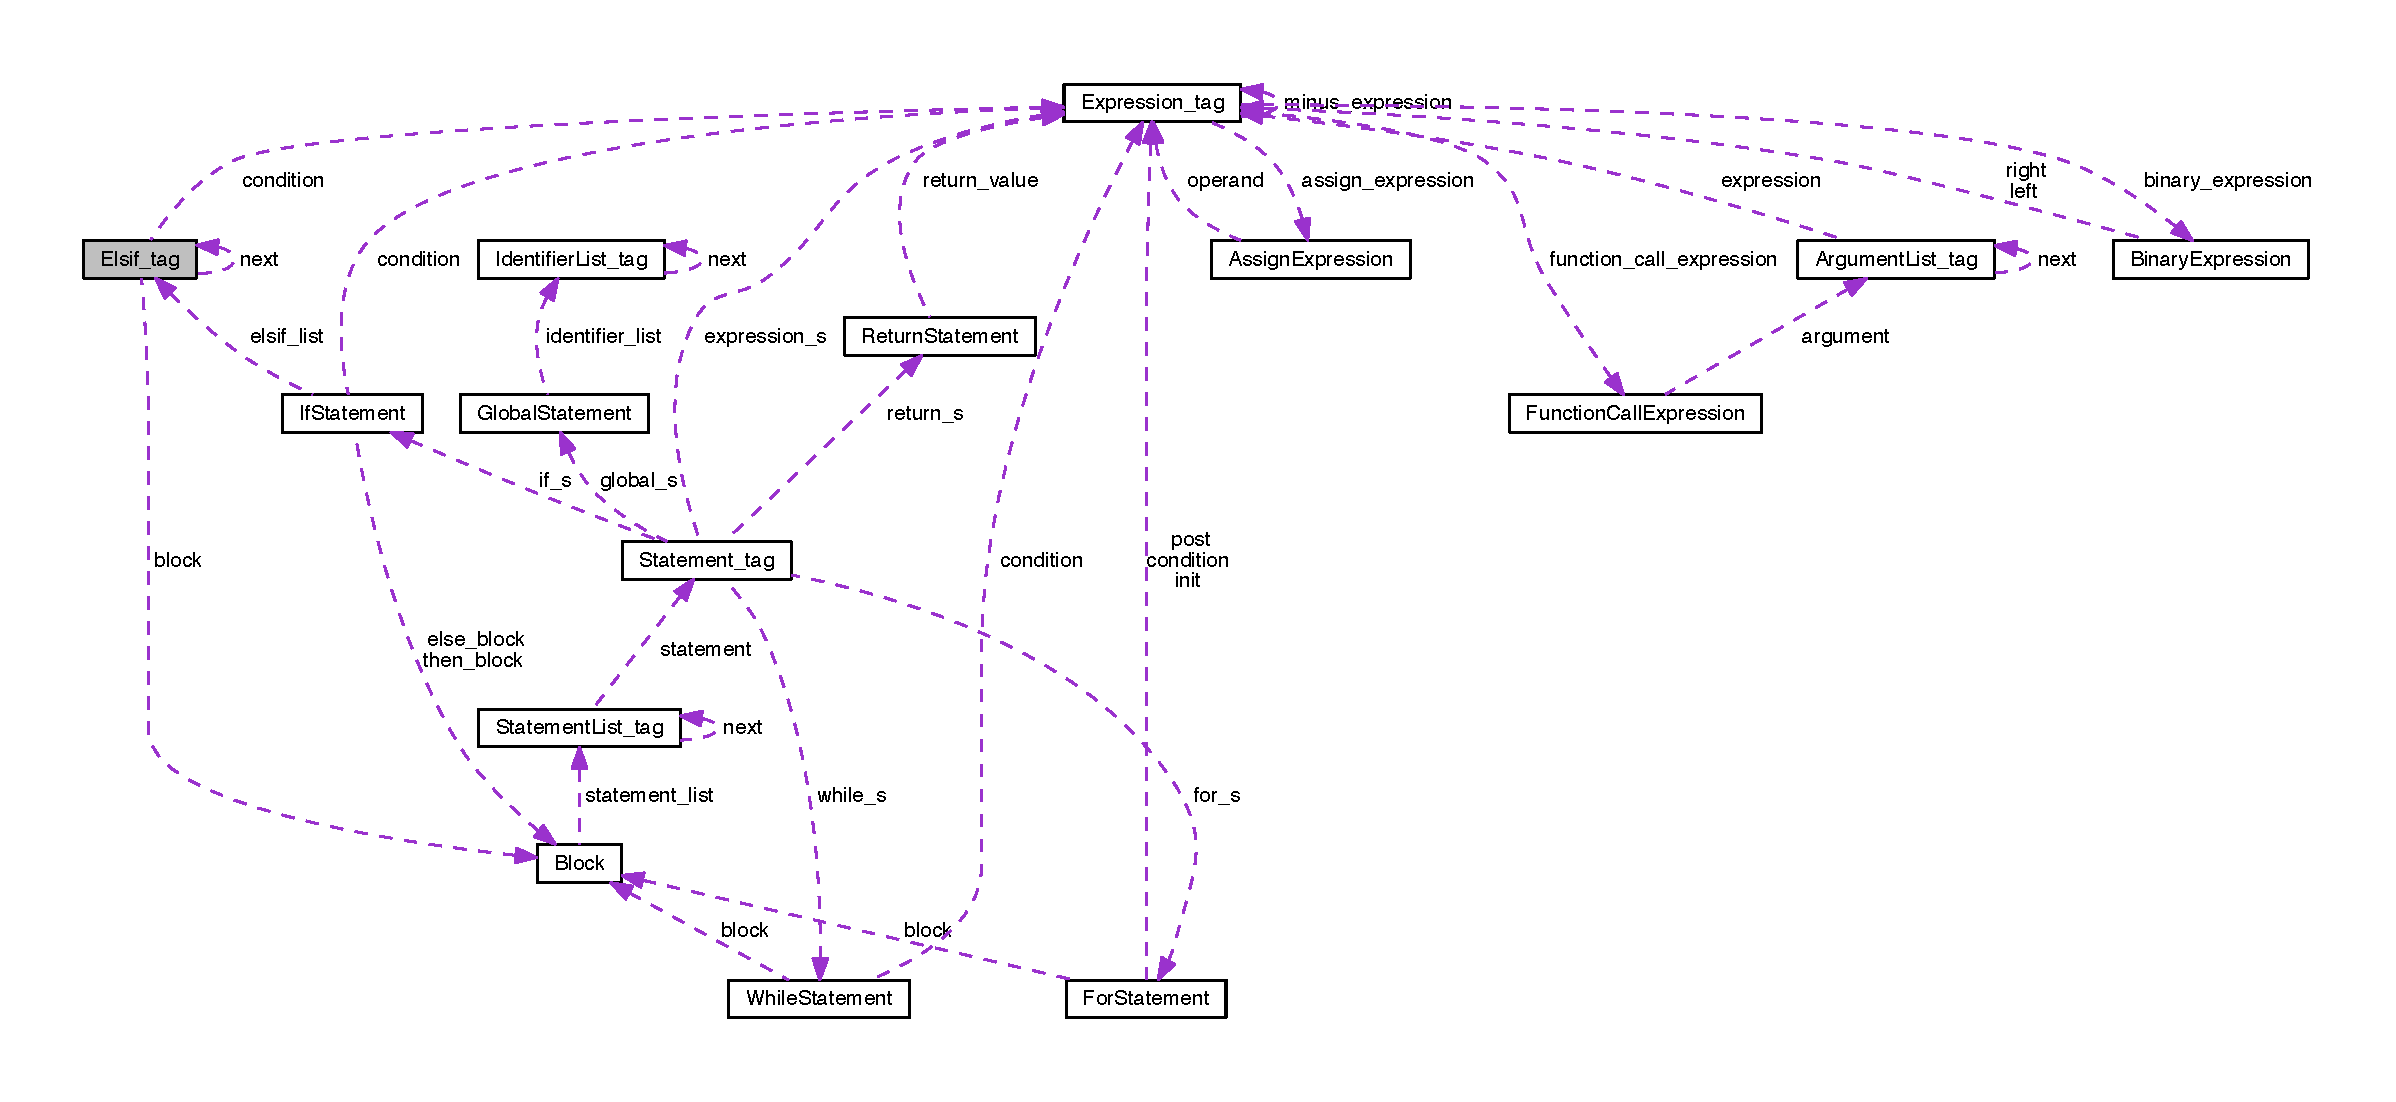
\includegraphics[width=350pt]{struct_elsif__tag__coll__graph}
\end{center}
\end{figure}
\subsection*{Public Attributes}
\begin{DoxyCompactItemize}
\item 
\hyperlink{crowbar_8h_a070c6feb370aad8a9665ca315bf6ed4a}{Expression} $\ast$ \hyperlink{struct_elsif__tag_a90add539e16a341fa17d195711585561}{condition}
\item 
\hyperlink{struct_block}{Block} $\ast$ \hyperlink{struct_elsif__tag_a9194a341db2b2733748ce1d7b9ad6dd9}{block}
\item 
struct \hyperlink{struct_elsif__tag}{Elsif\+\_\+tag} $\ast$ \hyperlink{struct_elsif__tag_a8a3bbc2610b58f08517837ee97da2549}{next}
\end{DoxyCompactItemize}


\subsection{Member Data Documentation}
\hypertarget{struct_elsif__tag_a9194a341db2b2733748ce1d7b9ad6dd9}{}\index{Elsif\+\_\+tag@{Elsif\+\_\+tag}!block@{block}}
\index{block@{block}!Elsif\+\_\+tag@{Elsif\+\_\+tag}}
\subsubsection[{block}]{\setlength{\rightskip}{0pt plus 5cm}{\bf Block}$\ast$ Elsif\+\_\+tag\+::block}\label{struct_elsif__tag_a9194a341db2b2733748ce1d7b9ad6dd9}
\hypertarget{struct_elsif__tag_a90add539e16a341fa17d195711585561}{}\index{Elsif\+\_\+tag@{Elsif\+\_\+tag}!condition@{condition}}
\index{condition@{condition}!Elsif\+\_\+tag@{Elsif\+\_\+tag}}
\subsubsection[{condition}]{\setlength{\rightskip}{0pt plus 5cm}{\bf Expression}$\ast$ Elsif\+\_\+tag\+::condition}\label{struct_elsif__tag_a90add539e16a341fa17d195711585561}
\hypertarget{struct_elsif__tag_a8a3bbc2610b58f08517837ee97da2549}{}\index{Elsif\+\_\+tag@{Elsif\+\_\+tag}!next@{next}}
\index{next@{next}!Elsif\+\_\+tag@{Elsif\+\_\+tag}}
\subsubsection[{next}]{\setlength{\rightskip}{0pt plus 5cm}struct {\bf Elsif\+\_\+tag}$\ast$ Elsif\+\_\+tag\+::next}\label{struct_elsif__tag_a8a3bbc2610b58f08517837ee97da2549}


The documentation for this struct was generated from the following file\+:\begin{DoxyCompactItemize}
\item 
\hyperlink{crowbar_8h}{crowbar.\+h}\end{DoxyCompactItemize}

\hypertarget{struct_expression__tag}{}\section{Expression\+\_\+tag Struct Reference}
\label{struct_expression__tag}\index{Expression\+\_\+tag@{Expression\+\_\+tag}}


{\ttfamily \#include $<$crowbar.\+h$>$}



Collaboration diagram for Expression\+\_\+tag\+:\nopagebreak
\begin{figure}[H]
\begin{center}
\leavevmode
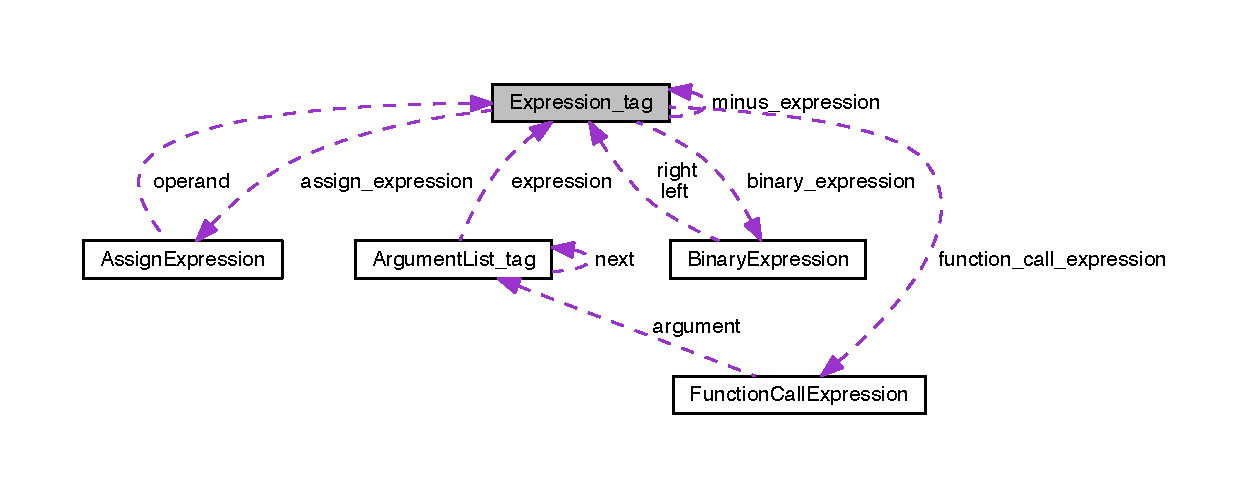
\includegraphics[width=350pt]{struct_expression__tag__coll__graph}
\end{center}
\end{figure}
\subsection*{Public Attributes}
\begin{DoxyCompactItemize}
\item 
\hyperlink{crowbar_8h_a51ad9989dafb48362f7e9354d68fe720}{Expression\+Type} \hyperlink{struct_expression__tag_a6e554d04874c28168b1294ad4860c2dc}{type}
\item 
int \hyperlink{struct_expression__tag_a00e220318941223a55e140e8ed0abff8}{line\+\_\+number}
\item 
\begin{tabbing}
xx\=xx\=xx\=xx\=xx\=xx\=xx\=xx\=xx\=\kill
union \{\\
\>\hyperlink{_c_r_b__dev_8h_a5000f2b447c9132c07d7f1cf66134a69}{CRB\_Boolean} \hyperlink{struct_expression__tag_aab2eb6d343ff191cb3017ae63a3588e3}{boolean\_value}\\
\>int \hyperlink{struct_expression__tag_a5b693b70a19d0fcd9a59861f71c14d7d}{int\_value}\\
\>double \hyperlink{struct_expression__tag_a23f1bc42ce2726e7c1ab776e88e2529e}{double\_value}\\
\>char $\ast$ \hyperlink{struct_expression__tag_a850dde0947b60a3a0a0aaf1d1509bbe1}{string\_value}\\
\>char $\ast$ \hyperlink{struct_expression__tag_a135bf93dc623a22f1f6eab611d65efc4}{identifier}\\
\>\hyperlink{struct_assign_expression}{AssignExpression} \hyperlink{struct_expression__tag_a889fe74ac3b67e574a1117850019aaad}{assign\_expression}\\
\>\hyperlink{struct_binary_expression}{BinaryExpression} \hyperlink{struct_expression__tag_aa855e521467183437ce1e72cc6bca675}{binary\_expression}\\
\>\hyperlink{crowbar_8h_a070c6feb370aad8a9665ca315bf6ed4a}{Expression} $\ast$ \hyperlink{struct_expression__tag_a87097a9f90ba91c0ff09983029b582e9}{minus\_expression}\\
\>\hyperlink{struct_function_call_expression}{FunctionCallExpression} \hyperlink{struct_expression__tag_ad1e62b0e65d2885da97209927845d444}{function\_call\_expression}\\
\} \hyperlink{struct_expression__tag_a0bb1fed3e5d9b4a6601d6783eb6bb9c3}{u}\\

\end{tabbing}\end{DoxyCompactItemize}


\subsection{Member Data Documentation}
\hypertarget{struct_expression__tag_a889fe74ac3b67e574a1117850019aaad}{}\index{Expression\+\_\+tag@{Expression\+\_\+tag}!assign\+\_\+expression@{assign\+\_\+expression}}
\index{assign\+\_\+expression@{assign\+\_\+expression}!Expression\+\_\+tag@{Expression\+\_\+tag}}
\subsubsection[{assign\+\_\+expression}]{\setlength{\rightskip}{0pt plus 5cm}{\bf Assign\+Expression} Expression\+\_\+tag\+::assign\+\_\+expression}\label{struct_expression__tag_a889fe74ac3b67e574a1117850019aaad}
\hypertarget{struct_expression__tag_aa855e521467183437ce1e72cc6bca675}{}\index{Expression\+\_\+tag@{Expression\+\_\+tag}!binary\+\_\+expression@{binary\+\_\+expression}}
\index{binary\+\_\+expression@{binary\+\_\+expression}!Expression\+\_\+tag@{Expression\+\_\+tag}}
\subsubsection[{binary\+\_\+expression}]{\setlength{\rightskip}{0pt plus 5cm}{\bf Binary\+Expression} Expression\+\_\+tag\+::binary\+\_\+expression}\label{struct_expression__tag_aa855e521467183437ce1e72cc6bca675}
\hypertarget{struct_expression__tag_aab2eb6d343ff191cb3017ae63a3588e3}{}\index{Expression\+\_\+tag@{Expression\+\_\+tag}!boolean\+\_\+value@{boolean\+\_\+value}}
\index{boolean\+\_\+value@{boolean\+\_\+value}!Expression\+\_\+tag@{Expression\+\_\+tag}}
\subsubsection[{boolean\+\_\+value}]{\setlength{\rightskip}{0pt plus 5cm}{\bf C\+R\+B\+\_\+\+Boolean} Expression\+\_\+tag\+::boolean\+\_\+value}\label{struct_expression__tag_aab2eb6d343ff191cb3017ae63a3588e3}
\hypertarget{struct_expression__tag_a23f1bc42ce2726e7c1ab776e88e2529e}{}\index{Expression\+\_\+tag@{Expression\+\_\+tag}!double\+\_\+value@{double\+\_\+value}}
\index{double\+\_\+value@{double\+\_\+value}!Expression\+\_\+tag@{Expression\+\_\+tag}}
\subsubsection[{double\+\_\+value}]{\setlength{\rightskip}{0pt plus 5cm}double Expression\+\_\+tag\+::double\+\_\+value}\label{struct_expression__tag_a23f1bc42ce2726e7c1ab776e88e2529e}
\hypertarget{struct_expression__tag_ad1e62b0e65d2885da97209927845d444}{}\index{Expression\+\_\+tag@{Expression\+\_\+tag}!function\+\_\+call\+\_\+expression@{function\+\_\+call\+\_\+expression}}
\index{function\+\_\+call\+\_\+expression@{function\+\_\+call\+\_\+expression}!Expression\+\_\+tag@{Expression\+\_\+tag}}
\subsubsection[{function\+\_\+call\+\_\+expression}]{\setlength{\rightskip}{0pt plus 5cm}{\bf Function\+Call\+Expression} Expression\+\_\+tag\+::function\+\_\+call\+\_\+expression}\label{struct_expression__tag_ad1e62b0e65d2885da97209927845d444}
\hypertarget{struct_expression__tag_a135bf93dc623a22f1f6eab611d65efc4}{}\index{Expression\+\_\+tag@{Expression\+\_\+tag}!identifier@{identifier}}
\index{identifier@{identifier}!Expression\+\_\+tag@{Expression\+\_\+tag}}
\subsubsection[{identifier}]{\setlength{\rightskip}{0pt plus 5cm}char$\ast$ Expression\+\_\+tag\+::identifier}\label{struct_expression__tag_a135bf93dc623a22f1f6eab611d65efc4}
\hypertarget{struct_expression__tag_a5b693b70a19d0fcd9a59861f71c14d7d}{}\index{Expression\+\_\+tag@{Expression\+\_\+tag}!int\+\_\+value@{int\+\_\+value}}
\index{int\+\_\+value@{int\+\_\+value}!Expression\+\_\+tag@{Expression\+\_\+tag}}
\subsubsection[{int\+\_\+value}]{\setlength{\rightskip}{0pt plus 5cm}int Expression\+\_\+tag\+::int\+\_\+value}\label{struct_expression__tag_a5b693b70a19d0fcd9a59861f71c14d7d}
\hypertarget{struct_expression__tag_a00e220318941223a55e140e8ed0abff8}{}\index{Expression\+\_\+tag@{Expression\+\_\+tag}!line\+\_\+number@{line\+\_\+number}}
\index{line\+\_\+number@{line\+\_\+number}!Expression\+\_\+tag@{Expression\+\_\+tag}}
\subsubsection[{line\+\_\+number}]{\setlength{\rightskip}{0pt plus 5cm}int Expression\+\_\+tag\+::line\+\_\+number}\label{struct_expression__tag_a00e220318941223a55e140e8ed0abff8}
\hypertarget{struct_expression__tag_a87097a9f90ba91c0ff09983029b582e9}{}\index{Expression\+\_\+tag@{Expression\+\_\+tag}!minus\+\_\+expression@{minus\+\_\+expression}}
\index{minus\+\_\+expression@{minus\+\_\+expression}!Expression\+\_\+tag@{Expression\+\_\+tag}}
\subsubsection[{minus\+\_\+expression}]{\setlength{\rightskip}{0pt plus 5cm}{\bf Expression}$\ast$ Expression\+\_\+tag\+::minus\+\_\+expression}\label{struct_expression__tag_a87097a9f90ba91c0ff09983029b582e9}
\hypertarget{struct_expression__tag_a850dde0947b60a3a0a0aaf1d1509bbe1}{}\index{Expression\+\_\+tag@{Expression\+\_\+tag}!string\+\_\+value@{string\+\_\+value}}
\index{string\+\_\+value@{string\+\_\+value}!Expression\+\_\+tag@{Expression\+\_\+tag}}
\subsubsection[{string\+\_\+value}]{\setlength{\rightskip}{0pt plus 5cm}char$\ast$ Expression\+\_\+tag\+::string\+\_\+value}\label{struct_expression__tag_a850dde0947b60a3a0a0aaf1d1509bbe1}
\hypertarget{struct_expression__tag_a6e554d04874c28168b1294ad4860c2dc}{}\index{Expression\+\_\+tag@{Expression\+\_\+tag}!type@{type}}
\index{type@{type}!Expression\+\_\+tag@{Expression\+\_\+tag}}
\subsubsection[{type}]{\setlength{\rightskip}{0pt plus 5cm}{\bf Expression\+Type} Expression\+\_\+tag\+::type}\label{struct_expression__tag_a6e554d04874c28168b1294ad4860c2dc}
\hypertarget{struct_expression__tag_a0bb1fed3e5d9b4a6601d6783eb6bb9c3}{}\index{Expression\+\_\+tag@{Expression\+\_\+tag}!u@{u}}
\index{u@{u}!Expression\+\_\+tag@{Expression\+\_\+tag}}
\subsubsection[{u}]{\setlength{\rightskip}{0pt plus 5cm}union \{ ... \}   Expression\+\_\+tag\+::u}\label{struct_expression__tag_a0bb1fed3e5d9b4a6601d6783eb6bb9c3}


The documentation for this struct was generated from the following file\+:\begin{DoxyCompactItemize}
\item 
\hyperlink{crowbar_8h}{crowbar.\+h}\end{DoxyCompactItemize}

\hypertarget{struct_for_statement}{}\section{For\+Statement Struct Reference}
\label{struct_for_statement}\index{For\+Statement@{For\+Statement}}


{\ttfamily \#include $<$crowbar.\+h$>$}



Collaboration diagram for For\+Statement\+:\nopagebreak
\begin{figure}[H]
\begin{center}
\leavevmode
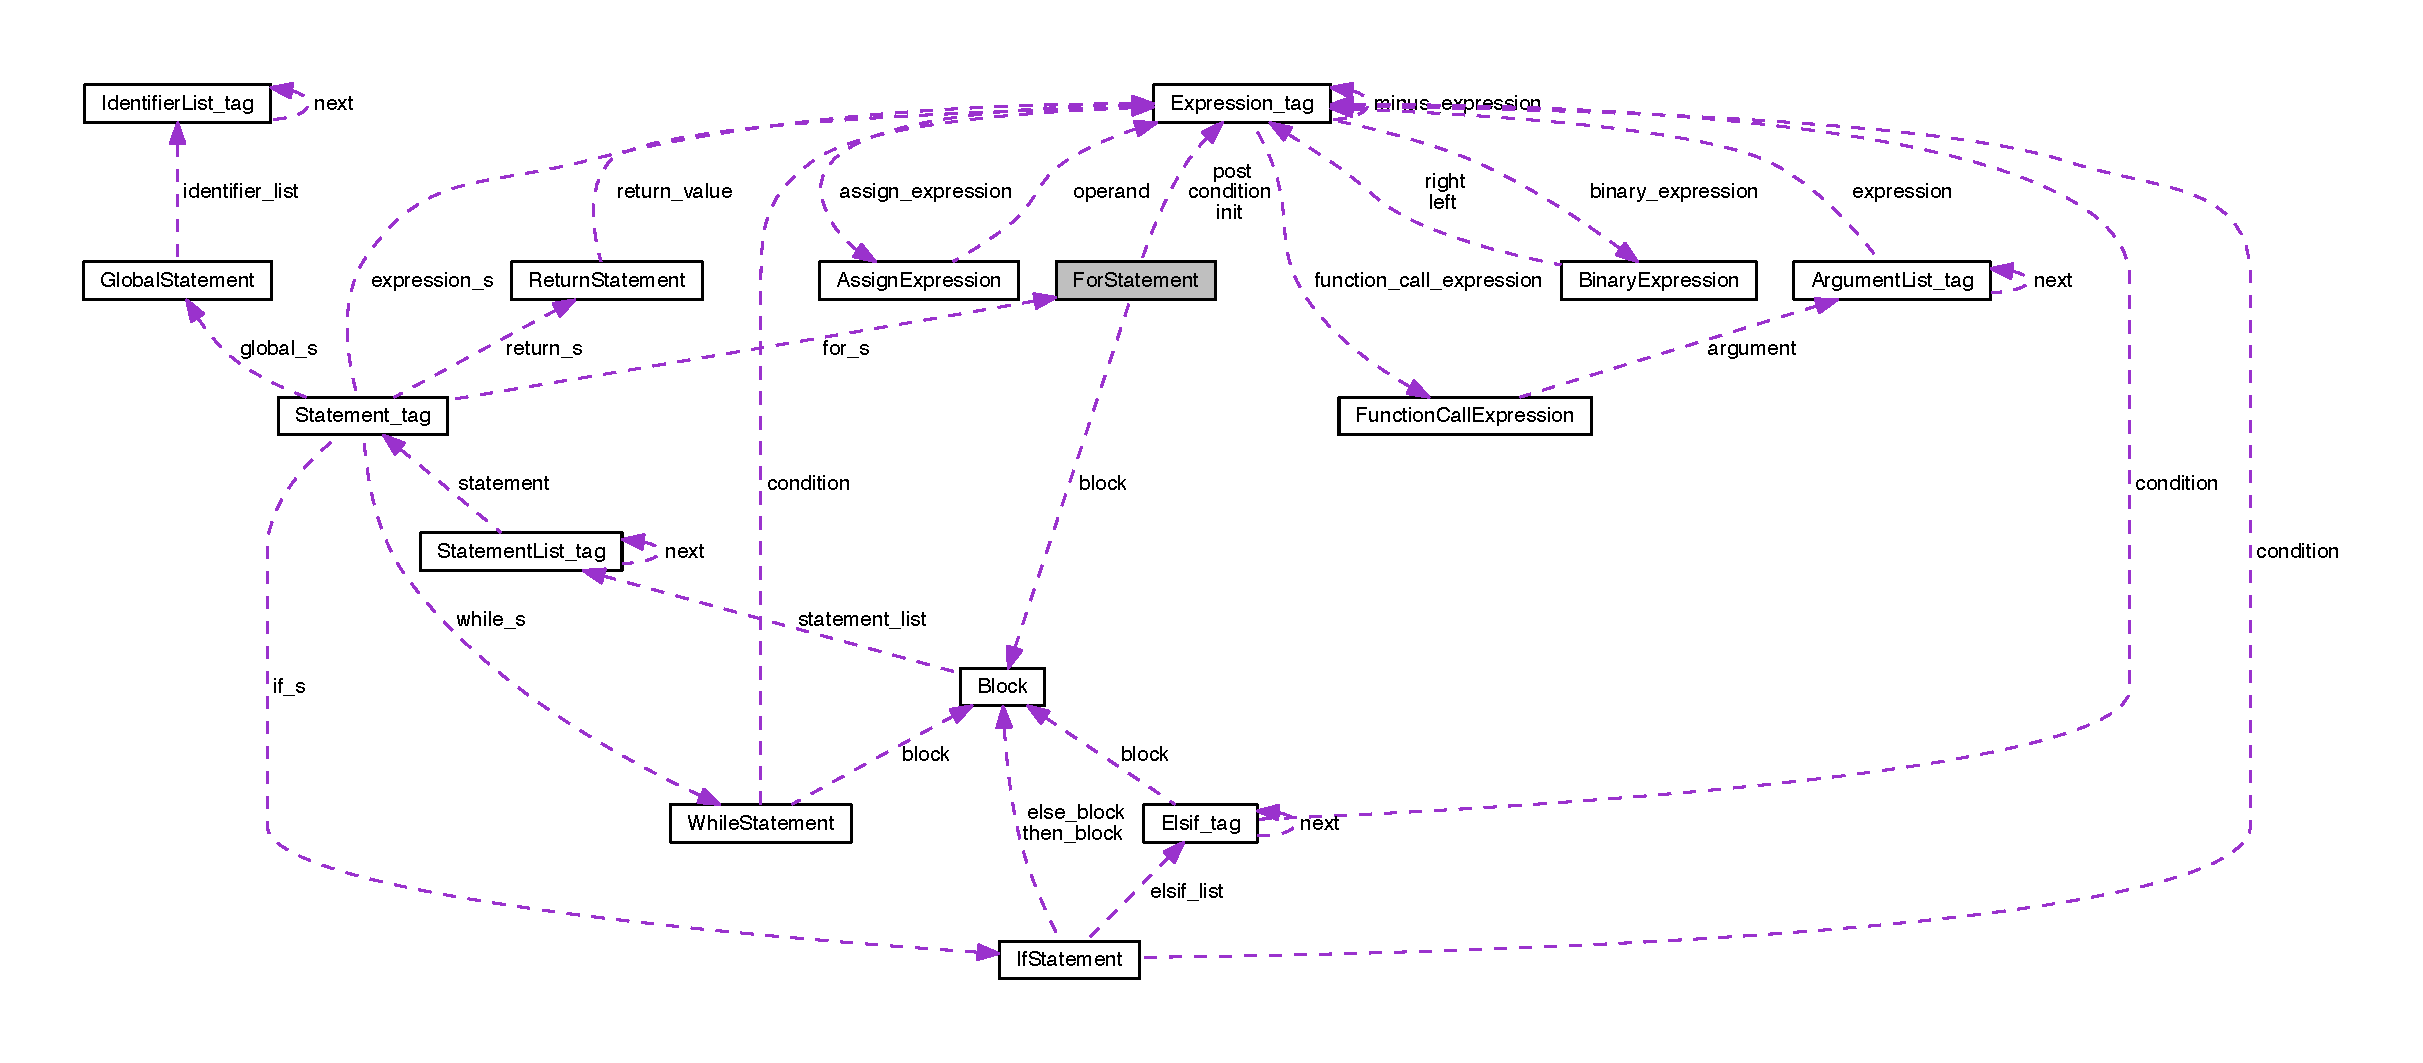
\includegraphics[width=350pt]{struct_for_statement__coll__graph}
\end{center}
\end{figure}
\subsection*{Public Attributes}
\begin{DoxyCompactItemize}
\item 
\hyperlink{crowbar_8h_a070c6feb370aad8a9665ca315bf6ed4a}{Expression} $\ast$ \hyperlink{struct_for_statement_ad651b9f23924d2f0aa19d4269353b526}{init}
\item 
\hyperlink{crowbar_8h_a070c6feb370aad8a9665ca315bf6ed4a}{Expression} $\ast$ \hyperlink{struct_for_statement_ada11b70a235641ef62d953293d00d7ba}{condition}
\item 
\hyperlink{crowbar_8h_a070c6feb370aad8a9665ca315bf6ed4a}{Expression} $\ast$ \hyperlink{struct_for_statement_a17a10be0a7696c064a0aa7e55e680903}{post}
\item 
\hyperlink{struct_block}{Block} $\ast$ \hyperlink{struct_for_statement_a482b9507e4e7064b2a3449106528d422}{block}
\end{DoxyCompactItemize}


\subsection{Member Data Documentation}
\hypertarget{struct_for_statement_a482b9507e4e7064b2a3449106528d422}{}\index{For\+Statement@{For\+Statement}!block@{block}}
\index{block@{block}!For\+Statement@{For\+Statement}}
\subsubsection[{block}]{\setlength{\rightskip}{0pt plus 5cm}{\bf Block}$\ast$ For\+Statement\+::block}\label{struct_for_statement_a482b9507e4e7064b2a3449106528d422}
\hypertarget{struct_for_statement_ada11b70a235641ef62d953293d00d7ba}{}\index{For\+Statement@{For\+Statement}!condition@{condition}}
\index{condition@{condition}!For\+Statement@{For\+Statement}}
\subsubsection[{condition}]{\setlength{\rightskip}{0pt plus 5cm}{\bf Expression}$\ast$ For\+Statement\+::condition}\label{struct_for_statement_ada11b70a235641ef62d953293d00d7ba}
\hypertarget{struct_for_statement_ad651b9f23924d2f0aa19d4269353b526}{}\index{For\+Statement@{For\+Statement}!init@{init}}
\index{init@{init}!For\+Statement@{For\+Statement}}
\subsubsection[{init}]{\setlength{\rightskip}{0pt plus 5cm}{\bf Expression}$\ast$ For\+Statement\+::init}\label{struct_for_statement_ad651b9f23924d2f0aa19d4269353b526}
\hypertarget{struct_for_statement_a17a10be0a7696c064a0aa7e55e680903}{}\index{For\+Statement@{For\+Statement}!post@{post}}
\index{post@{post}!For\+Statement@{For\+Statement}}
\subsubsection[{post}]{\setlength{\rightskip}{0pt plus 5cm}{\bf Expression}$\ast$ For\+Statement\+::post}\label{struct_for_statement_a17a10be0a7696c064a0aa7e55e680903}


The documentation for this struct was generated from the following file\+:\begin{DoxyCompactItemize}
\item 
\hyperlink{crowbar_8h}{crowbar.\+h}\end{DoxyCompactItemize}

\hypertarget{struct_function_call_expression}{}\section{Function\+Call\+Expression Struct Reference}
\label{struct_function_call_expression}\index{Function\+Call\+Expression@{Function\+Call\+Expression}}


{\ttfamily \#include $<$crowbar.\+h$>$}



Collaboration diagram for Function\+Call\+Expression\+:\nopagebreak
\begin{figure}[H]
\begin{center}
\leavevmode
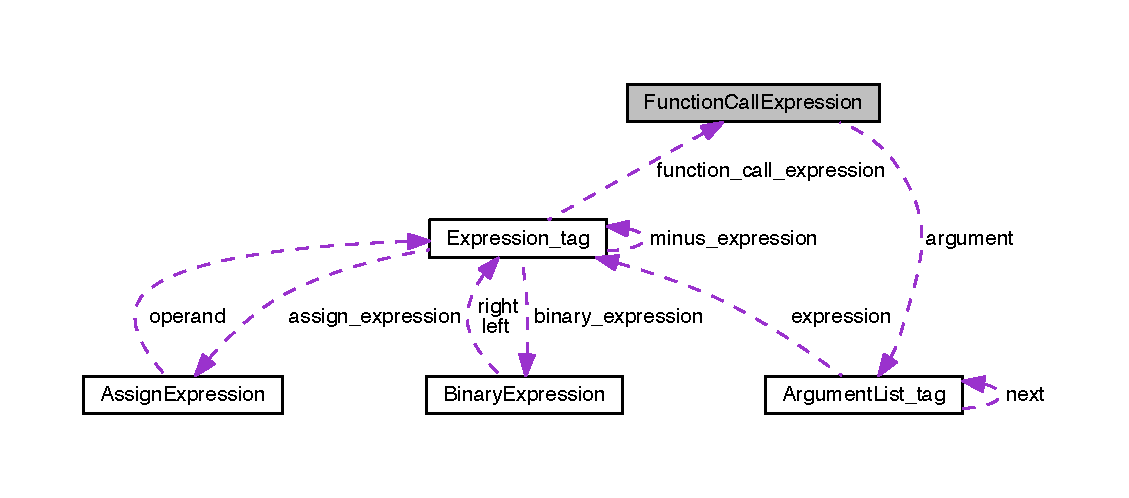
\includegraphics[width=350pt]{struct_function_call_expression__coll__graph}
\end{center}
\end{figure}
\subsection*{Public Attributes}
\begin{DoxyCompactItemize}
\item 
char $\ast$ \hyperlink{struct_function_call_expression_a9c3a09de854a826e104f65297edd184b}{identifier}
\item 
\hyperlink{crowbar_8h_ad4ba12ca8ae3ead90081fb0aba63aff3}{Argument\+List} $\ast$ \hyperlink{struct_function_call_expression_a278e6d5a95113ab48d019026c4e5641d}{argument}
\end{DoxyCompactItemize}


\subsection{Member Data Documentation}
\hypertarget{struct_function_call_expression_a278e6d5a95113ab48d019026c4e5641d}{}\index{Function\+Call\+Expression@{Function\+Call\+Expression}!argument@{argument}}
\index{argument@{argument}!Function\+Call\+Expression@{Function\+Call\+Expression}}
\subsubsection[{argument}]{\setlength{\rightskip}{0pt plus 5cm}{\bf Argument\+List}$\ast$ Function\+Call\+Expression\+::argument}\label{struct_function_call_expression_a278e6d5a95113ab48d019026c4e5641d}
\hypertarget{struct_function_call_expression_a9c3a09de854a826e104f65297edd184b}{}\index{Function\+Call\+Expression@{Function\+Call\+Expression}!identifier@{identifier}}
\index{identifier@{identifier}!Function\+Call\+Expression@{Function\+Call\+Expression}}
\subsubsection[{identifier}]{\setlength{\rightskip}{0pt plus 5cm}char$\ast$ Function\+Call\+Expression\+::identifier}\label{struct_function_call_expression_a9c3a09de854a826e104f65297edd184b}


The documentation for this struct was generated from the following file\+:\begin{DoxyCompactItemize}
\item 
\hyperlink{crowbar_8h}{crowbar.\+h}\end{DoxyCompactItemize}

\hypertarget{struct_function_definition__tag}{}\section{Function\+Definition\+\_\+tag Struct Reference}
\label{struct_function_definition__tag}\index{Function\+Definition\+\_\+tag@{Function\+Definition\+\_\+tag}}


{\ttfamily \#include $<$crowbar.\+h$>$}



Collaboration diagram for Function\+Definition\+\_\+tag\+:\nopagebreak
\begin{figure}[H]
\begin{center}
\leavevmode
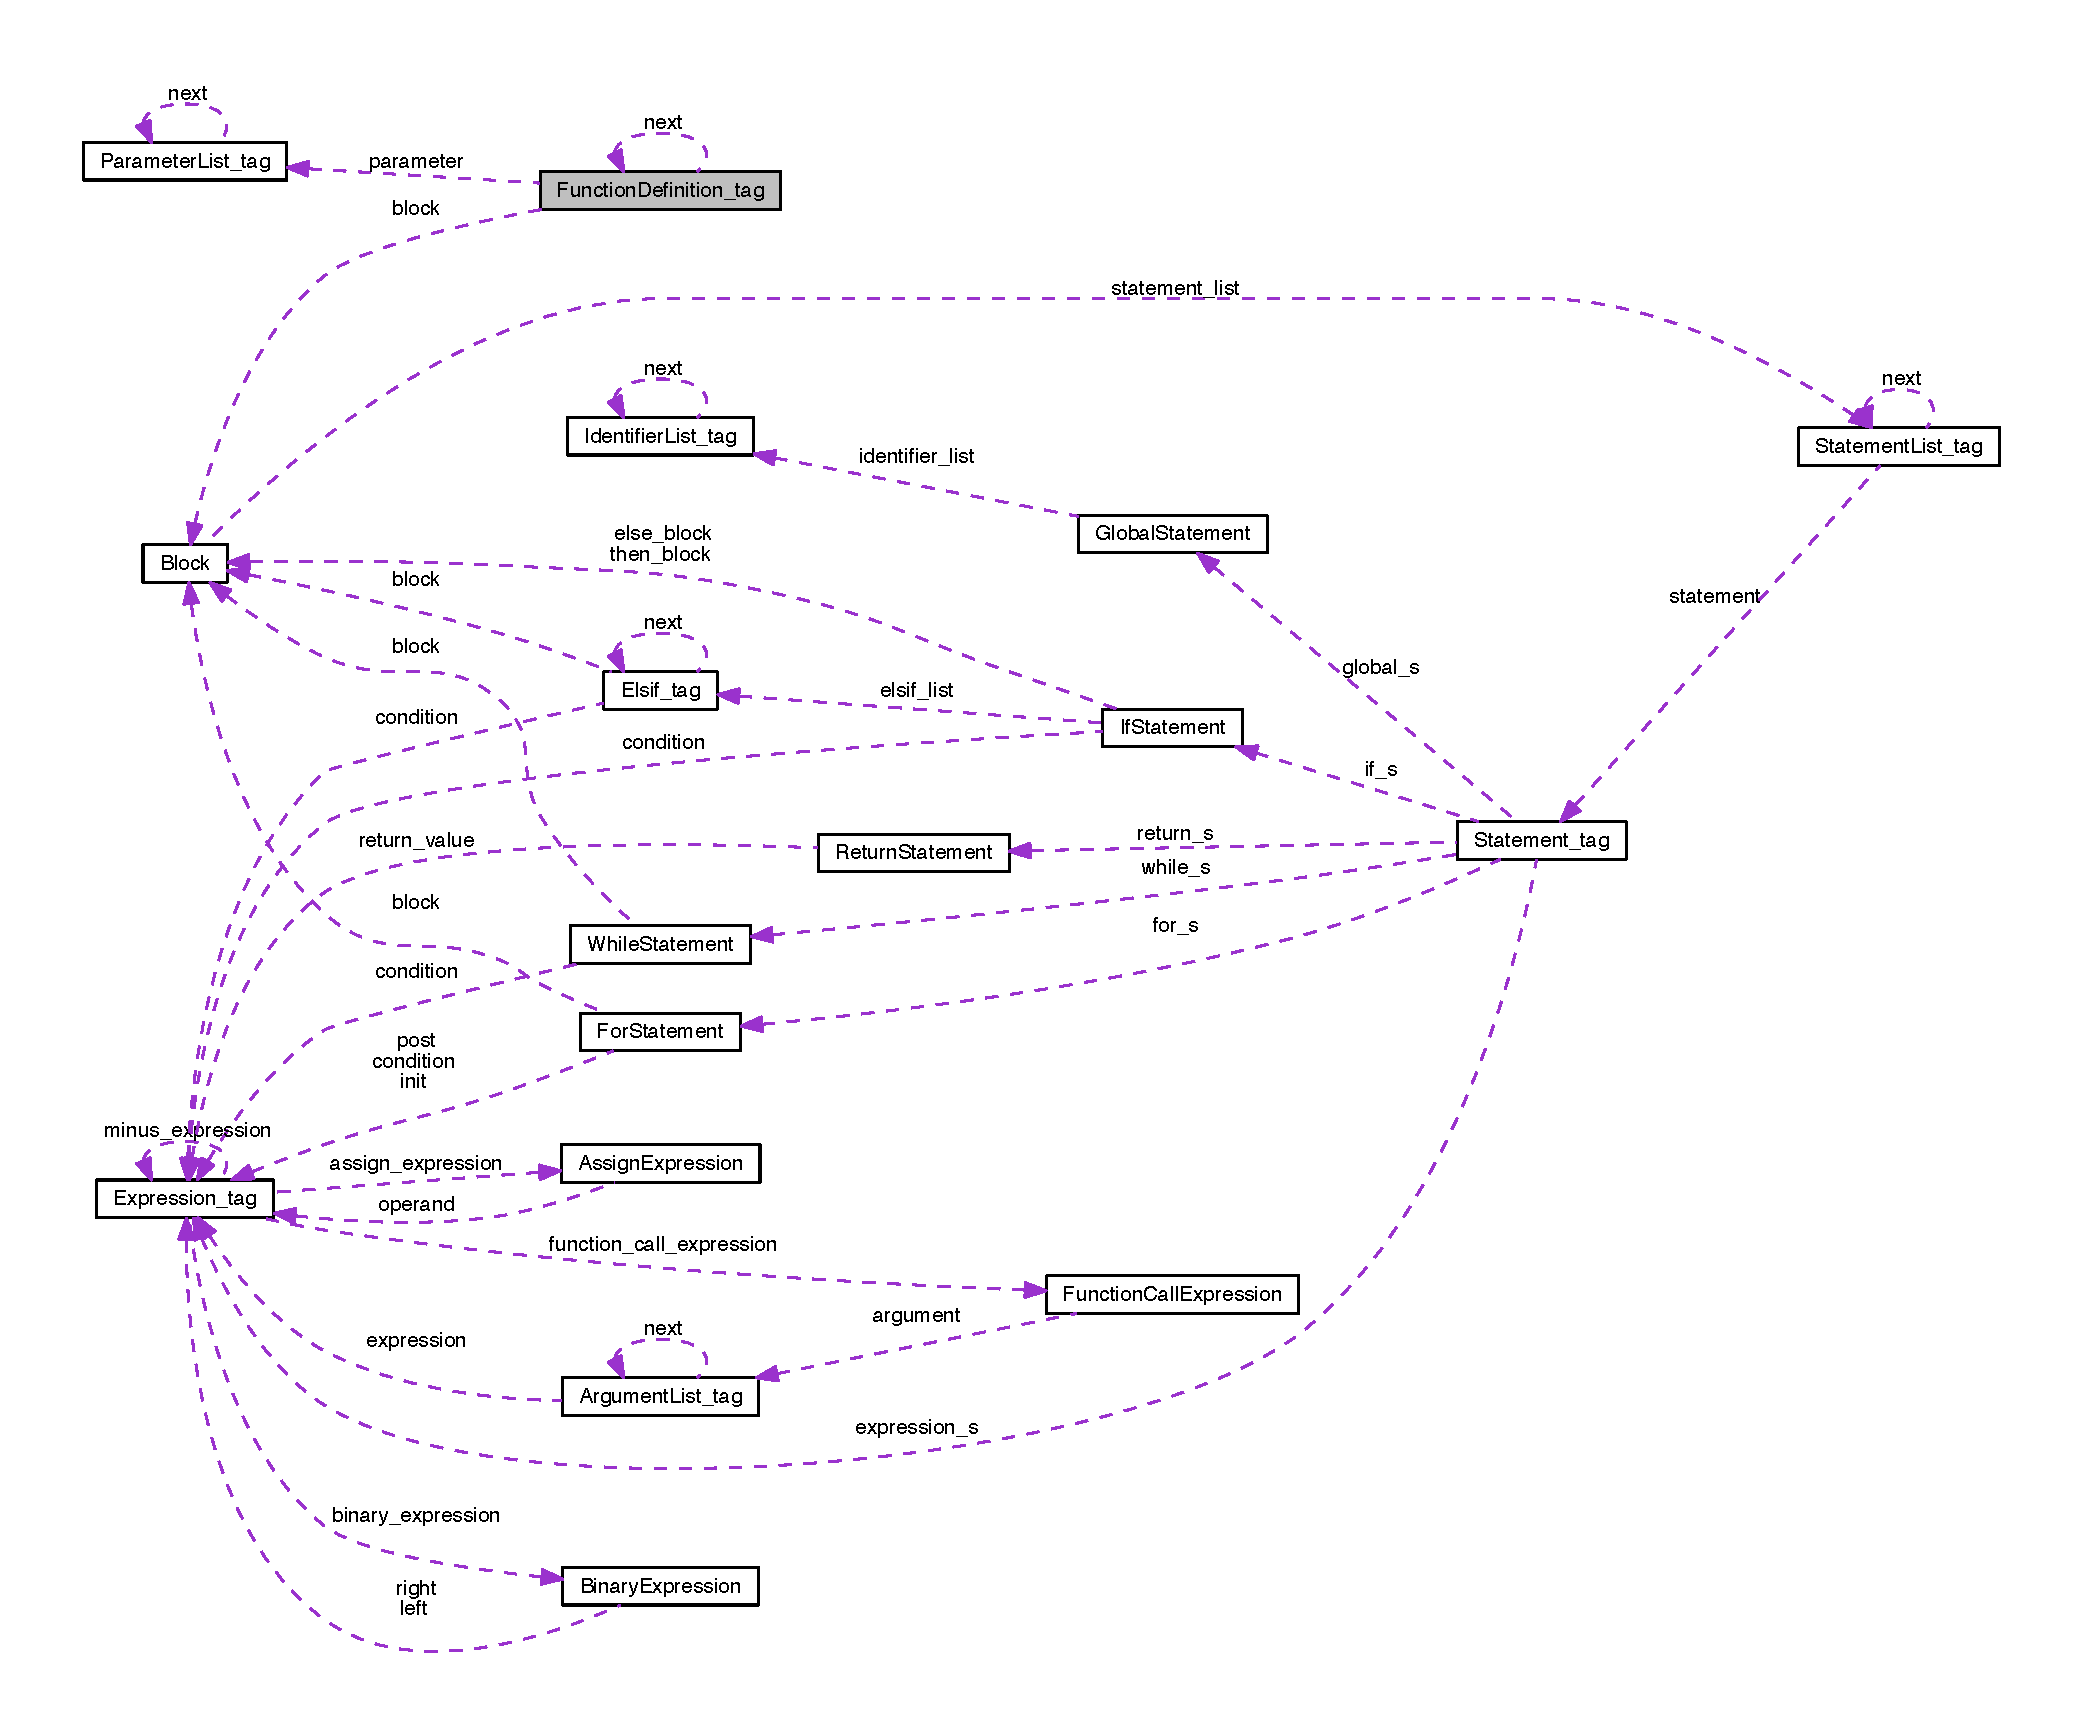
\includegraphics[width=350pt]{struct_function_definition__tag__coll__graph}
\end{center}
\end{figure}
\subsection*{Public Attributes}
\begin{DoxyCompactItemize}
\item 
char $\ast$ \hyperlink{struct_function_definition__tag_ac86d561cdc103d16dc92445651fbde2f}{name}
\item 
\hyperlink{crowbar_8h_a67222f1cbccd1a26edc686500aa6ea97}{Function\+Definition\+Type} \hyperlink{struct_function_definition__tag_a6477190ea35ab3daa69aa8762e302661}{type}
\item 
\begin{tabbing}
xx\=xx\=xx\=xx\=xx\=xx\=xx\=xx\=xx\=\kill
union \{\\
\>struct \{\\
\>\>\hyperlink{crowbar_8h_a7e7687e26b28e339ebcc8eaab571dcf7}{ParameterList} $\ast$ \hyperlink{struct_function_definition__tag_a920e515da65f6d48e75864181108dba4}{parameter}\\
\>\>\hyperlink{struct_block}{Block} $\ast$ \hyperlink{struct_function_definition__tag_a63493f81a30a92680126bbb0a6331816}{block}\\
\>\} \hyperlink{struct_function_definition__tag_ac903298e1aeddc0d693b5591f3f127e3}{crowbar\_f}\\
\>struct \{\\
\>\>\hyperlink{_c_r_b__dev_8h_af310ef1ce709cc9c2e7d1e3bf43b76ec}{CRB\_NativeFunctionProc} $\ast$ \hyperlink{struct_function_definition__tag_a5178ea679186f4c16f227644e060c350}{proc}\\
\>\} \hyperlink{struct_function_definition__tag_a47669f5b5a90c174a8074dcee352b889}{native\_f}\\
\} \hyperlink{struct_function_definition__tag_a82459859fdf1587b0bf434c5e9c61192}{u}\\

\end{tabbing}\item 
struct \hyperlink{struct_function_definition__tag}{Function\+Definition\+\_\+tag} $\ast$ \hyperlink{struct_function_definition__tag_ab9569f0ddbe305b4c58fdc673f0afd01}{next}
\end{DoxyCompactItemize}


\subsection{Member Data Documentation}
\hypertarget{struct_function_definition__tag_a63493f81a30a92680126bbb0a6331816}{}\index{Function\+Definition\+\_\+tag@{Function\+Definition\+\_\+tag}!block@{block}}
\index{block@{block}!Function\+Definition\+\_\+tag@{Function\+Definition\+\_\+tag}}
\subsubsection[{block}]{\setlength{\rightskip}{0pt plus 5cm}{\bf Block}$\ast$ Function\+Definition\+\_\+tag\+::block}\label{struct_function_definition__tag_a63493f81a30a92680126bbb0a6331816}
\hypertarget{struct_function_definition__tag_ac903298e1aeddc0d693b5591f3f127e3}{}\index{Function\+Definition\+\_\+tag@{Function\+Definition\+\_\+tag}!crowbar\+\_\+f@{crowbar\+\_\+f}}
\index{crowbar\+\_\+f@{crowbar\+\_\+f}!Function\+Definition\+\_\+tag@{Function\+Definition\+\_\+tag}}
\subsubsection[{crowbar\+\_\+f}]{\setlength{\rightskip}{0pt plus 5cm}struct \{ ... \}   Function\+Definition\+\_\+tag\+::crowbar\+\_\+f}\label{struct_function_definition__tag_ac903298e1aeddc0d693b5591f3f127e3}
\hypertarget{struct_function_definition__tag_ac86d561cdc103d16dc92445651fbde2f}{}\index{Function\+Definition\+\_\+tag@{Function\+Definition\+\_\+tag}!name@{name}}
\index{name@{name}!Function\+Definition\+\_\+tag@{Function\+Definition\+\_\+tag}}
\subsubsection[{name}]{\setlength{\rightskip}{0pt plus 5cm}char$\ast$ Function\+Definition\+\_\+tag\+::name}\label{struct_function_definition__tag_ac86d561cdc103d16dc92445651fbde2f}
\hypertarget{struct_function_definition__tag_a47669f5b5a90c174a8074dcee352b889}{}\index{Function\+Definition\+\_\+tag@{Function\+Definition\+\_\+tag}!native\+\_\+f@{native\+\_\+f}}
\index{native\+\_\+f@{native\+\_\+f}!Function\+Definition\+\_\+tag@{Function\+Definition\+\_\+tag}}
\subsubsection[{native\+\_\+f}]{\setlength{\rightskip}{0pt plus 5cm}struct \{ ... \}   Function\+Definition\+\_\+tag\+::native\+\_\+f}\label{struct_function_definition__tag_a47669f5b5a90c174a8074dcee352b889}
\hypertarget{struct_function_definition__tag_ab9569f0ddbe305b4c58fdc673f0afd01}{}\index{Function\+Definition\+\_\+tag@{Function\+Definition\+\_\+tag}!next@{next}}
\index{next@{next}!Function\+Definition\+\_\+tag@{Function\+Definition\+\_\+tag}}
\subsubsection[{next}]{\setlength{\rightskip}{0pt plus 5cm}struct {\bf Function\+Definition\+\_\+tag}$\ast$ Function\+Definition\+\_\+tag\+::next}\label{struct_function_definition__tag_ab9569f0ddbe305b4c58fdc673f0afd01}
\hypertarget{struct_function_definition__tag_a920e515da65f6d48e75864181108dba4}{}\index{Function\+Definition\+\_\+tag@{Function\+Definition\+\_\+tag}!parameter@{parameter}}
\index{parameter@{parameter}!Function\+Definition\+\_\+tag@{Function\+Definition\+\_\+tag}}
\subsubsection[{parameter}]{\setlength{\rightskip}{0pt plus 5cm}{\bf Parameter\+List}$\ast$ Function\+Definition\+\_\+tag\+::parameter}\label{struct_function_definition__tag_a920e515da65f6d48e75864181108dba4}
\hypertarget{struct_function_definition__tag_a5178ea679186f4c16f227644e060c350}{}\index{Function\+Definition\+\_\+tag@{Function\+Definition\+\_\+tag}!proc@{proc}}
\index{proc@{proc}!Function\+Definition\+\_\+tag@{Function\+Definition\+\_\+tag}}
\subsubsection[{proc}]{\setlength{\rightskip}{0pt plus 5cm}{\bf C\+R\+B\+\_\+\+Native\+Function\+Proc}$\ast$ Function\+Definition\+\_\+tag\+::proc}\label{struct_function_definition__tag_a5178ea679186f4c16f227644e060c350}
\hypertarget{struct_function_definition__tag_a6477190ea35ab3daa69aa8762e302661}{}\index{Function\+Definition\+\_\+tag@{Function\+Definition\+\_\+tag}!type@{type}}
\index{type@{type}!Function\+Definition\+\_\+tag@{Function\+Definition\+\_\+tag}}
\subsubsection[{type}]{\setlength{\rightskip}{0pt plus 5cm}{\bf Function\+Definition\+Type} Function\+Definition\+\_\+tag\+::type}\label{struct_function_definition__tag_a6477190ea35ab3daa69aa8762e302661}
\hypertarget{struct_function_definition__tag_a82459859fdf1587b0bf434c5e9c61192}{}\index{Function\+Definition\+\_\+tag@{Function\+Definition\+\_\+tag}!u@{u}}
\index{u@{u}!Function\+Definition\+\_\+tag@{Function\+Definition\+\_\+tag}}
\subsubsection[{u}]{\setlength{\rightskip}{0pt plus 5cm}union \{ ... \}   Function\+Definition\+\_\+tag\+::u}\label{struct_function_definition__tag_a82459859fdf1587b0bf434c5e9c61192}


The documentation for this struct was generated from the following file\+:\begin{DoxyCompactItemize}
\item 
\hyperlink{crowbar_8h}{crowbar.\+h}\end{DoxyCompactItemize}

\hypertarget{struct_global_statement}{}\section{Global\+Statement Struct Reference}
\label{struct_global_statement}\index{Global\+Statement@{Global\+Statement}}


{\ttfamily \#include $<$crowbar.\+h$>$}



Collaboration diagram for Global\+Statement\+:\nopagebreak
\begin{figure}[H]
\begin{center}
\leavevmode
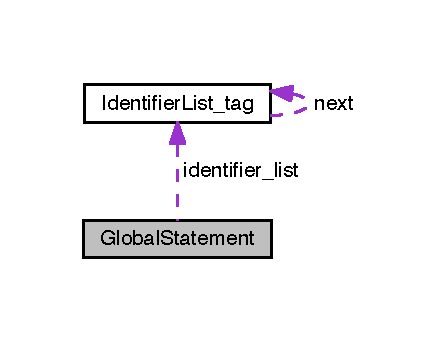
\includegraphics[width=210pt]{struct_global_statement__coll__graph}
\end{center}
\end{figure}
\subsection*{Public Attributes}
\begin{DoxyCompactItemize}
\item 
\hyperlink{crowbar_8h_a3e8fd423ff4b73a7c5d557375f0a8741}{Identifier\+List} $\ast$ \hyperlink{struct_global_statement_a5d68fa84111ef8d6ed16dc7f3dbdd2ab}{identifier\+\_\+list}
\end{DoxyCompactItemize}


\subsection{Member Data Documentation}
\hypertarget{struct_global_statement_a5d68fa84111ef8d6ed16dc7f3dbdd2ab}{}\index{Global\+Statement@{Global\+Statement}!identifier\+\_\+list@{identifier\+\_\+list}}
\index{identifier\+\_\+list@{identifier\+\_\+list}!Global\+Statement@{Global\+Statement}}
\subsubsection[{identifier\+\_\+list}]{\setlength{\rightskip}{0pt plus 5cm}{\bf Identifier\+List}$\ast$ Global\+Statement\+::identifier\+\_\+list}\label{struct_global_statement_a5d68fa84111ef8d6ed16dc7f3dbdd2ab}


The documentation for this struct was generated from the following file\+:\begin{DoxyCompactItemize}
\item 
\hyperlink{crowbar_8h}{crowbar.\+h}\end{DoxyCompactItemize}

\hypertarget{struct_global_variable_ref__tag}{}\section{Global\+Variable\+Ref\+\_\+tag Struct Reference}
\label{struct_global_variable_ref__tag}\index{Global\+Variable\+Ref\+\_\+tag@{Global\+Variable\+Ref\+\_\+tag}}


{\ttfamily \#include $<$crowbar.\+h$>$}



Collaboration diagram for Global\+Variable\+Ref\+\_\+tag\+:\nopagebreak
\begin{figure}[H]
\begin{center}
\leavevmode
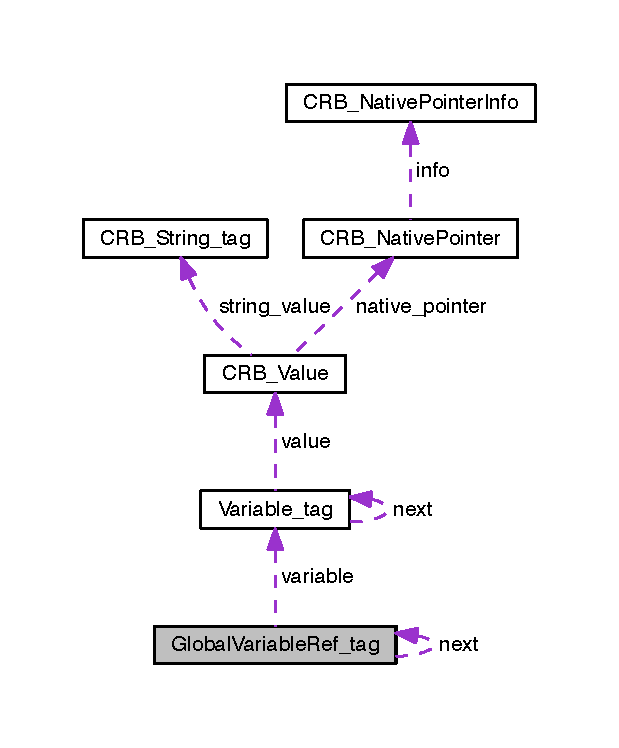
\includegraphics[width=297pt]{struct_global_variable_ref__tag__coll__graph}
\end{center}
\end{figure}
\subsection*{Public Attributes}
\begin{DoxyCompactItemize}
\item 
\hyperlink{crowbar_8h_a070c86ad7ae39536aed471927d04dee4}{Variable} $\ast$ \hyperlink{struct_global_variable_ref__tag_aa1dd1472b8328df21455bffc4d2a4c12}{variable}
\item 
struct \hyperlink{struct_global_variable_ref__tag}{Global\+Variable\+Ref\+\_\+tag} $\ast$ \hyperlink{struct_global_variable_ref__tag_aaadfe23f53ea5a6ed782d89a689cf47d}{next}
\end{DoxyCompactItemize}


\subsection{Member Data Documentation}
\hypertarget{struct_global_variable_ref__tag_aaadfe23f53ea5a6ed782d89a689cf47d}{}\index{Global\+Variable\+Ref\+\_\+tag@{Global\+Variable\+Ref\+\_\+tag}!next@{next}}
\index{next@{next}!Global\+Variable\+Ref\+\_\+tag@{Global\+Variable\+Ref\+\_\+tag}}
\subsubsection[{next}]{\setlength{\rightskip}{0pt plus 5cm}struct {\bf Global\+Variable\+Ref\+\_\+tag}$\ast$ Global\+Variable\+Ref\+\_\+tag\+::next}\label{struct_global_variable_ref__tag_aaadfe23f53ea5a6ed782d89a689cf47d}
\hypertarget{struct_global_variable_ref__tag_aa1dd1472b8328df21455bffc4d2a4c12}{}\index{Global\+Variable\+Ref\+\_\+tag@{Global\+Variable\+Ref\+\_\+tag}!variable@{variable}}
\index{variable@{variable}!Global\+Variable\+Ref\+\_\+tag@{Global\+Variable\+Ref\+\_\+tag}}
\subsubsection[{variable}]{\setlength{\rightskip}{0pt plus 5cm}{\bf Variable}$\ast$ Global\+Variable\+Ref\+\_\+tag\+::variable}\label{struct_global_variable_ref__tag_aa1dd1472b8328df21455bffc4d2a4c12}


The documentation for this struct was generated from the following file\+:\begin{DoxyCompactItemize}
\item 
\hyperlink{crowbar_8h}{crowbar.\+h}\end{DoxyCompactItemize}

\hypertarget{union_header__tag}{}\section{Header\+\_\+tag Union Reference}
\label{union_header__tag}\index{Header\+\_\+tag@{Header\+\_\+tag}}


Collaboration diagram for Header\+\_\+tag\+:\nopagebreak
\begin{figure}[H]
\begin{center}
\leavevmode
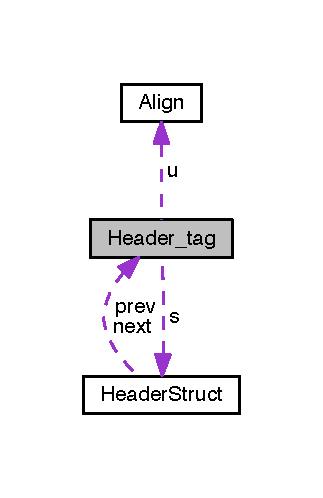
\includegraphics[width=155pt]{union_header__tag__coll__graph}
\end{center}
\end{figure}
\subsection*{Public Attributes}
\begin{DoxyCompactItemize}
\item 
\hyperlink{struct_header_struct}{Header\+Struct} \hyperlink{union_header__tag_a9431ea46df35bb4feca322cb96246bab}{s}
\item 
\hyperlink{union_align}{Align} \hyperlink{union_header__tag_a5fbc38dfa9adcb54937811882ea1e8b3}{u} \mbox{[}\hyperlink{memory_8c_ad1b52843007ad984fe47a9e236305e74}{H\+E\+A\+D\+E\+R\+\_\+\+A\+L\+I\+G\+N\+\_\+\+S\+I\+Z\+E}\mbox{]}
\end{DoxyCompactItemize}


\subsection{Member Data Documentation}
\hypertarget{union_header__tag_a9431ea46df35bb4feca322cb96246bab}{}\index{Header\+\_\+tag@{Header\+\_\+tag}!s@{s}}
\index{s@{s}!Header\+\_\+tag@{Header\+\_\+tag}}
\subsubsection[{s}]{\setlength{\rightskip}{0pt plus 5cm}{\bf Header\+Struct} Header\+\_\+tag\+::s}\label{union_header__tag_a9431ea46df35bb4feca322cb96246bab}
\hypertarget{union_header__tag_a5fbc38dfa9adcb54937811882ea1e8b3}{}\index{Header\+\_\+tag@{Header\+\_\+tag}!u@{u}}
\index{u@{u}!Header\+\_\+tag@{Header\+\_\+tag}}
\subsubsection[{u}]{\setlength{\rightskip}{0pt plus 5cm}{\bf Align} Header\+\_\+tag\+::u\mbox{[}{\bf H\+E\+A\+D\+E\+R\+\_\+\+A\+L\+I\+G\+N\+\_\+\+S\+I\+Z\+E}\mbox{]}}\label{union_header__tag_a5fbc38dfa9adcb54937811882ea1e8b3}


The documentation for this union was generated from the following file\+:\begin{DoxyCompactItemize}
\item 
memory/\hyperlink{memory_8c}{memory.\+c}\end{DoxyCompactItemize}

\hypertarget{struct_header_struct}{}\section{Header\+Struct Struct Reference}
\label{struct_header_struct}\index{Header\+Struct@{Header\+Struct}}


Collaboration diagram for Header\+Struct\+:\nopagebreak
\begin{figure}[H]
\begin{center}
\leavevmode
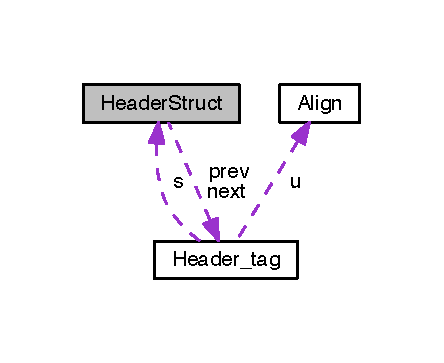
\includegraphics[width=213pt]{struct_header_struct__coll__graph}
\end{center}
\end{figure}
\subsection*{Public Attributes}
\begin{DoxyCompactItemize}
\item 
int \hyperlink{struct_header_struct_ad6b63ca7e387b292da71cf12e41b56ca}{size}
\item 
char $\ast$ \hyperlink{struct_header_struct_ac66081945a967351e1c465cf9fc1ad0e}{filename}
\item 
int \hyperlink{struct_header_struct_a598de0f5ec396866b1d534806ac93fb5}{line}
\item 
\hyperlink{memory_8h_a387a413b7c06fb892e5cc4a59fe7ed17}{Header} $\ast$ \hyperlink{struct_header_struct_a3071c07de335b54aaa6151adb871f8bf}{prev}
\item 
\hyperlink{memory_8h_a387a413b7c06fb892e5cc4a59fe7ed17}{Header} $\ast$ \hyperlink{struct_header_struct_adb09b99f377a7c151915ddd4b63eb2ae}{next}
\item 
unsigned char \hyperlink{struct_header_struct_aa7ff45e1bfc66ff72d9ffc41e4021447}{mark} \mbox{[}\hyperlink{memory_8c_a017f486cae1059db631df5f5c360d9f5}{M\+A\+R\+K\+\_\+\+S\+I\+Z\+E}\mbox{]}
\end{DoxyCompactItemize}


\subsection{Member Data Documentation}
\hypertarget{struct_header_struct_ac66081945a967351e1c465cf9fc1ad0e}{}\index{Header\+Struct@{Header\+Struct}!filename@{filename}}
\index{filename@{filename}!Header\+Struct@{Header\+Struct}}
\subsubsection[{filename}]{\setlength{\rightskip}{0pt plus 5cm}char$\ast$ Header\+Struct\+::filename}\label{struct_header_struct_ac66081945a967351e1c465cf9fc1ad0e}
\hypertarget{struct_header_struct_a598de0f5ec396866b1d534806ac93fb5}{}\index{Header\+Struct@{Header\+Struct}!line@{line}}
\index{line@{line}!Header\+Struct@{Header\+Struct}}
\subsubsection[{line}]{\setlength{\rightskip}{0pt plus 5cm}int Header\+Struct\+::line}\label{struct_header_struct_a598de0f5ec396866b1d534806ac93fb5}
\hypertarget{struct_header_struct_aa7ff45e1bfc66ff72d9ffc41e4021447}{}\index{Header\+Struct@{Header\+Struct}!mark@{mark}}
\index{mark@{mark}!Header\+Struct@{Header\+Struct}}
\subsubsection[{mark}]{\setlength{\rightskip}{0pt plus 5cm}unsigned char Header\+Struct\+::mark\mbox{[}{\bf M\+A\+R\+K\+\_\+\+S\+I\+Z\+E}\mbox{]}}\label{struct_header_struct_aa7ff45e1bfc66ff72d9ffc41e4021447}
\hypertarget{struct_header_struct_adb09b99f377a7c151915ddd4b63eb2ae}{}\index{Header\+Struct@{Header\+Struct}!next@{next}}
\index{next@{next}!Header\+Struct@{Header\+Struct}}
\subsubsection[{next}]{\setlength{\rightskip}{0pt plus 5cm}{\bf Header}$\ast$ Header\+Struct\+::next}\label{struct_header_struct_adb09b99f377a7c151915ddd4b63eb2ae}
\hypertarget{struct_header_struct_a3071c07de335b54aaa6151adb871f8bf}{}\index{Header\+Struct@{Header\+Struct}!prev@{prev}}
\index{prev@{prev}!Header\+Struct@{Header\+Struct}}
\subsubsection[{prev}]{\setlength{\rightskip}{0pt plus 5cm}{\bf Header}$\ast$ Header\+Struct\+::prev}\label{struct_header_struct_a3071c07de335b54aaa6151adb871f8bf}
\hypertarget{struct_header_struct_ad6b63ca7e387b292da71cf12e41b56ca}{}\index{Header\+Struct@{Header\+Struct}!size@{size}}
\index{size@{size}!Header\+Struct@{Header\+Struct}}
\subsubsection[{size}]{\setlength{\rightskip}{0pt plus 5cm}int Header\+Struct\+::size}\label{struct_header_struct_ad6b63ca7e387b292da71cf12e41b56ca}


The documentation for this struct was generated from the following file\+:\begin{DoxyCompactItemize}
\item 
memory/\hyperlink{memory_8c}{memory.\+c}\end{DoxyCompactItemize}

\hypertarget{struct_identifier_list__tag}{}\section{Identifier\+List\+\_\+tag Struct Reference}
\label{struct_identifier_list__tag}\index{Identifier\+List\+\_\+tag@{Identifier\+List\+\_\+tag}}


{\ttfamily \#include $<$crowbar.\+h$>$}



Collaboration diagram for Identifier\+List\+\_\+tag\+:\nopagebreak
\begin{figure}[H]
\begin{center}
\leavevmode
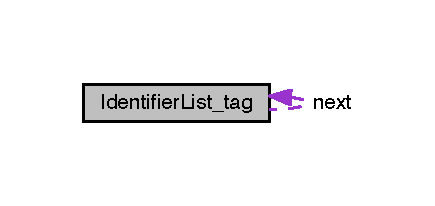
\includegraphics[width=209pt]{struct_identifier_list__tag__coll__graph}
\end{center}
\end{figure}
\subsection*{Public Attributes}
\begin{DoxyCompactItemize}
\item 
char $\ast$ \hyperlink{struct_identifier_list__tag_a35c08fe43ab2ee6ec72d10510a509a36}{name}
\item 
struct \hyperlink{struct_identifier_list__tag}{Identifier\+List\+\_\+tag} $\ast$ \hyperlink{struct_identifier_list__tag_ab078cbf07ee9896784b46a0dca4ccb2d}{next}
\end{DoxyCompactItemize}


\subsection{Member Data Documentation}
\hypertarget{struct_identifier_list__tag_a35c08fe43ab2ee6ec72d10510a509a36}{}\index{Identifier\+List\+\_\+tag@{Identifier\+List\+\_\+tag}!name@{name}}
\index{name@{name}!Identifier\+List\+\_\+tag@{Identifier\+List\+\_\+tag}}
\subsubsection[{name}]{\setlength{\rightskip}{0pt plus 5cm}char$\ast$ Identifier\+List\+\_\+tag\+::name}\label{struct_identifier_list__tag_a35c08fe43ab2ee6ec72d10510a509a36}
\hypertarget{struct_identifier_list__tag_ab078cbf07ee9896784b46a0dca4ccb2d}{}\index{Identifier\+List\+\_\+tag@{Identifier\+List\+\_\+tag}!next@{next}}
\index{next@{next}!Identifier\+List\+\_\+tag@{Identifier\+List\+\_\+tag}}
\subsubsection[{next}]{\setlength{\rightskip}{0pt plus 5cm}struct {\bf Identifier\+List\+\_\+tag}$\ast$ Identifier\+List\+\_\+tag\+::next}\label{struct_identifier_list__tag_ab078cbf07ee9896784b46a0dca4ccb2d}


The documentation for this struct was generated from the following file\+:\begin{DoxyCompactItemize}
\item 
\hyperlink{crowbar_8h}{crowbar.\+h}\end{DoxyCompactItemize}

\hypertarget{struct_if_statement}{}\section{If\+Statement Struct Reference}
\label{struct_if_statement}\index{If\+Statement@{If\+Statement}}


{\ttfamily \#include $<$crowbar.\+h$>$}



Collaboration diagram for If\+Statement\+:\nopagebreak
\begin{figure}[H]
\begin{center}
\leavevmode
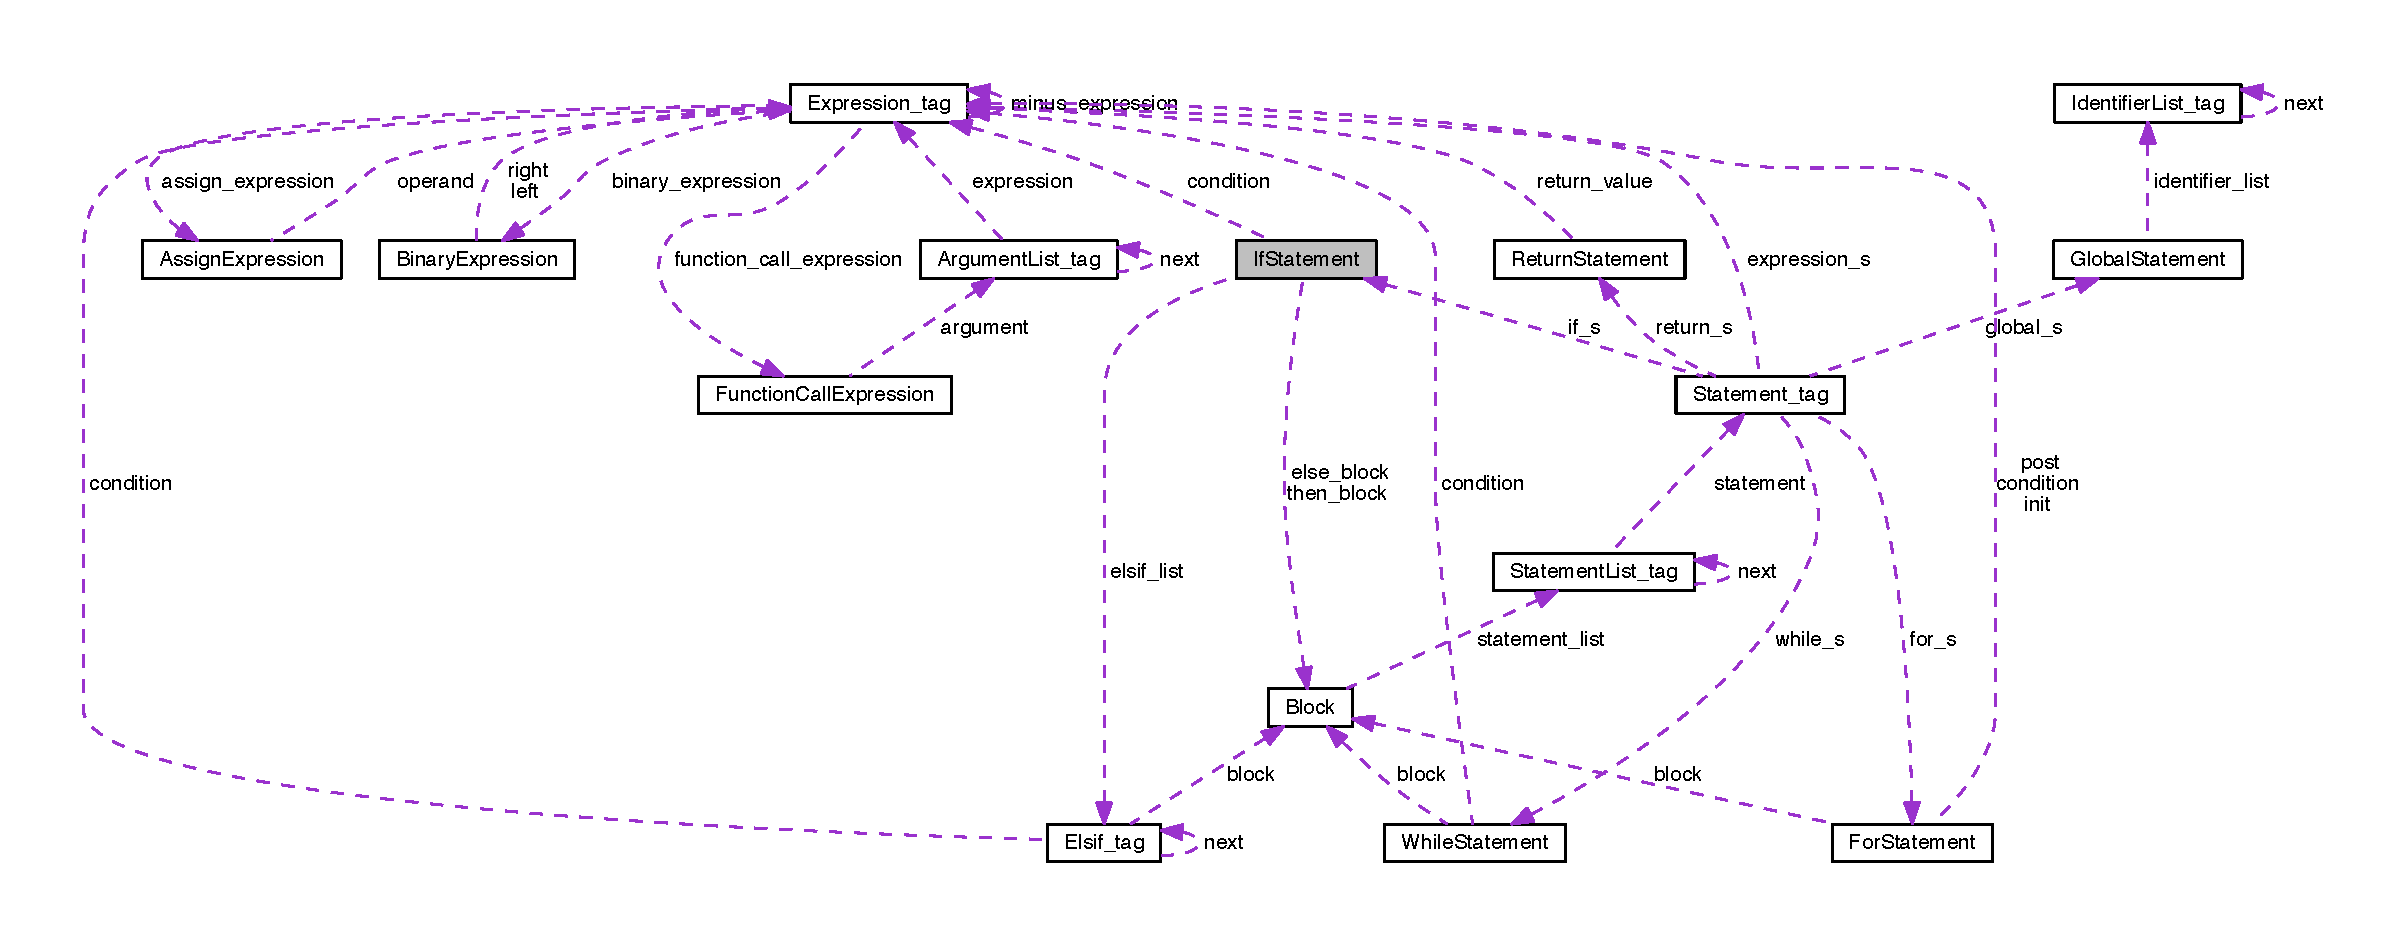
\includegraphics[width=350pt]{struct_if_statement__coll__graph}
\end{center}
\end{figure}
\subsection*{Public Attributes}
\begin{DoxyCompactItemize}
\item 
\hyperlink{crowbar_8h_a070c6feb370aad8a9665ca315bf6ed4a}{Expression} $\ast$ \hyperlink{struct_if_statement_a2f94ffdf006915378fd04adcca34decd}{condition}
\item 
\hyperlink{struct_block}{Block} $\ast$ \hyperlink{struct_if_statement_aa3ad1531bae5272926856f65fa9109a6}{then\+\_\+block}
\item 
\hyperlink{crowbar_8h_a8d2ba32155a8a8a5a87e93c564061f1d}{Elsif} $\ast$ \hyperlink{struct_if_statement_a9fca446be841301fe78695d38c69f5e5}{elsif\+\_\+list}
\item 
\hyperlink{struct_block}{Block} $\ast$ \hyperlink{struct_if_statement_ab2fa316c9e48259809b33d1551a072fa}{else\+\_\+block}
\end{DoxyCompactItemize}


\subsection{Member Data Documentation}
\hypertarget{struct_if_statement_a2f94ffdf006915378fd04adcca34decd}{}\index{If\+Statement@{If\+Statement}!condition@{condition}}
\index{condition@{condition}!If\+Statement@{If\+Statement}}
\subsubsection[{condition}]{\setlength{\rightskip}{0pt plus 5cm}{\bf Expression}$\ast$ If\+Statement\+::condition}\label{struct_if_statement_a2f94ffdf006915378fd04adcca34decd}
\hypertarget{struct_if_statement_ab2fa316c9e48259809b33d1551a072fa}{}\index{If\+Statement@{If\+Statement}!else\+\_\+block@{else\+\_\+block}}
\index{else\+\_\+block@{else\+\_\+block}!If\+Statement@{If\+Statement}}
\subsubsection[{else\+\_\+block}]{\setlength{\rightskip}{0pt plus 5cm}{\bf Block}$\ast$ If\+Statement\+::else\+\_\+block}\label{struct_if_statement_ab2fa316c9e48259809b33d1551a072fa}
\hypertarget{struct_if_statement_a9fca446be841301fe78695d38c69f5e5}{}\index{If\+Statement@{If\+Statement}!elsif\+\_\+list@{elsif\+\_\+list}}
\index{elsif\+\_\+list@{elsif\+\_\+list}!If\+Statement@{If\+Statement}}
\subsubsection[{elsif\+\_\+list}]{\setlength{\rightskip}{0pt plus 5cm}{\bf Elsif}$\ast$ If\+Statement\+::elsif\+\_\+list}\label{struct_if_statement_a9fca446be841301fe78695d38c69f5e5}
\hypertarget{struct_if_statement_aa3ad1531bae5272926856f65fa9109a6}{}\index{If\+Statement@{If\+Statement}!then\+\_\+block@{then\+\_\+block}}
\index{then\+\_\+block@{then\+\_\+block}!If\+Statement@{If\+Statement}}
\subsubsection[{then\+\_\+block}]{\setlength{\rightskip}{0pt plus 5cm}{\bf Block}$\ast$ If\+Statement\+::then\+\_\+block}\label{struct_if_statement_aa3ad1531bae5272926856f65fa9109a6}


The documentation for this struct was generated from the following file\+:\begin{DoxyCompactItemize}
\item 
\hyperlink{crowbar_8h}{crowbar.\+h}\end{DoxyCompactItemize}

\hypertarget{struct_local_environment}{}\section{Local\+Environment Struct Reference}
\label{struct_local_environment}\index{Local\+Environment@{Local\+Environment}}


{\ttfamily \#include $<$crowbar.\+h$>$}



Collaboration diagram for Local\+Environment\+:\nopagebreak
\begin{figure}[H]
\begin{center}
\leavevmode
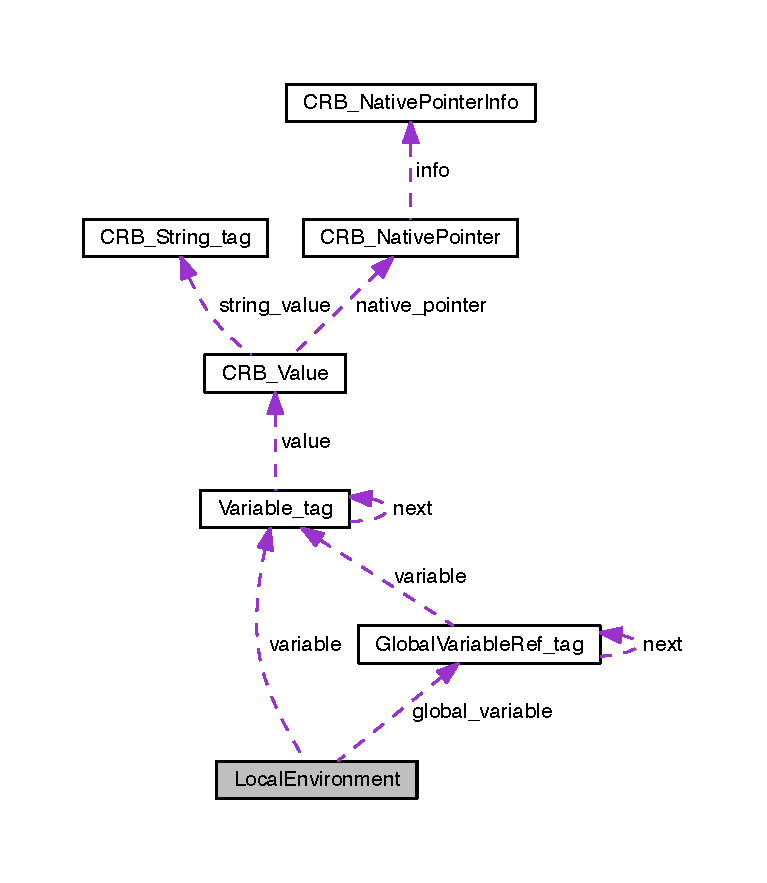
\includegraphics[width=350pt]{struct_local_environment__coll__graph}
\end{center}
\end{figure}
\subsection*{Public Attributes}
\begin{DoxyCompactItemize}
\item 
\hyperlink{crowbar_8h_a070c86ad7ae39536aed471927d04dee4}{Variable} $\ast$ \hyperlink{struct_local_environment_a80c4a3efddd4486c76844fb7f22bca1d}{variable}
\item 
\hyperlink{crowbar_8h_ac709ecd8d021425e844a82940d5d1028}{Global\+Variable\+Ref} $\ast$ \hyperlink{struct_local_environment_a4c244dd2fedac828d3db9e42a61772a1}{global\+\_\+variable}
\end{DoxyCompactItemize}


\subsection{Member Data Documentation}
\hypertarget{struct_local_environment_a4c244dd2fedac828d3db9e42a61772a1}{}\index{Local\+Environment@{Local\+Environment}!global\+\_\+variable@{global\+\_\+variable}}
\index{global\+\_\+variable@{global\+\_\+variable}!Local\+Environment@{Local\+Environment}}
\subsubsection[{global\+\_\+variable}]{\setlength{\rightskip}{0pt plus 5cm}{\bf Global\+Variable\+Ref}$\ast$ Local\+Environment\+::global\+\_\+variable}\label{struct_local_environment_a4c244dd2fedac828d3db9e42a61772a1}
\hypertarget{struct_local_environment_a80c4a3efddd4486c76844fb7f22bca1d}{}\index{Local\+Environment@{Local\+Environment}!variable@{variable}}
\index{variable@{variable}!Local\+Environment@{Local\+Environment}}
\subsubsection[{variable}]{\setlength{\rightskip}{0pt plus 5cm}{\bf Variable}$\ast$ Local\+Environment\+::variable}\label{struct_local_environment_a80c4a3efddd4486c76844fb7f22bca1d}


The documentation for this struct was generated from the following file\+:\begin{DoxyCompactItemize}
\item 
\hyperlink{crowbar_8h}{crowbar.\+h}\end{DoxyCompactItemize}

\hypertarget{struct_m_e_m___controller__tag}{}\section{M\+E\+M\+\_\+\+Controller\+\_\+tag Struct Reference}
\label{struct_m_e_m___controller__tag}\index{M\+E\+M\+\_\+\+Controller\+\_\+tag@{M\+E\+M\+\_\+\+Controller\+\_\+tag}}


{\ttfamily \#include $<$memory.\+h$>$}



Collaboration diagram for M\+E\+M\+\_\+\+Controller\+\_\+tag\+:\nopagebreak
\begin{figure}[H]
\begin{center}
\leavevmode
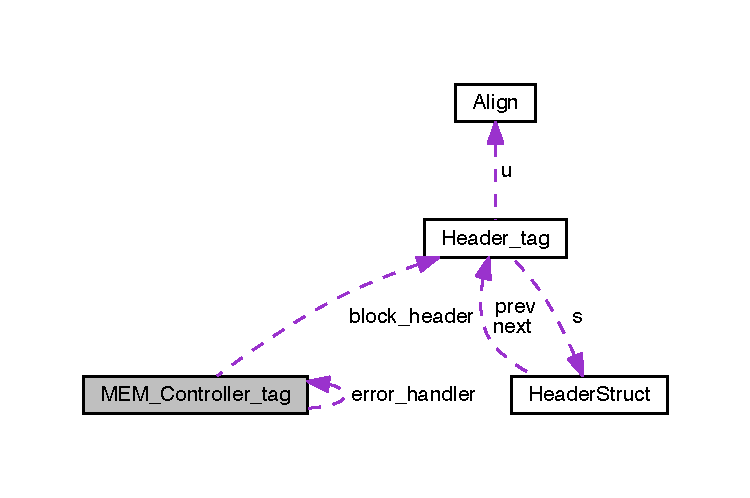
\includegraphics[width=350pt]{struct_m_e_m___controller__tag__coll__graph}
\end{center}
\end{figure}
\subsection*{Public Attributes}
\begin{DoxyCompactItemize}
\item 
F\+I\+L\+E $\ast$ \hyperlink{struct_m_e_m___controller__tag_a574de58b2a1928a04e5e7a7cbb1c2e37}{error\+\_\+fp}
\item 
\hyperlink{_m_e_m_8h_ade0991d07952a94a24685337fad1ca80}{M\+E\+M\+\_\+\+Error\+Handler} \hyperlink{struct_m_e_m___controller__tag_a8e66791a8c41fabb661c122942150dab}{error\+\_\+handler}
\item 
\hyperlink{_m_e_m_8h_ab9335a5fd03b90054312289c76acf8ca}{M\+E\+M\+\_\+\+Fail\+Mode} \hyperlink{struct_m_e_m___controller__tag_ac3d980809419cb5d423a4bcf8022d0c8}{fail\+\_\+mode}
\item 
\hyperlink{memory_8h_a387a413b7c06fb892e5cc4a59fe7ed17}{Header} $\ast$ \hyperlink{struct_m_e_m___controller__tag_a8cdf922b2df14ad5c169e8719d47e8fb}{block\+\_\+header}
\end{DoxyCompactItemize}


\subsection{Member Data Documentation}
\hypertarget{struct_m_e_m___controller__tag_a8cdf922b2df14ad5c169e8719d47e8fb}{}\index{M\+E\+M\+\_\+\+Controller\+\_\+tag@{M\+E\+M\+\_\+\+Controller\+\_\+tag}!block\+\_\+header@{block\+\_\+header}}
\index{block\+\_\+header@{block\+\_\+header}!M\+E\+M\+\_\+\+Controller\+\_\+tag@{M\+E\+M\+\_\+\+Controller\+\_\+tag}}
\subsubsection[{block\+\_\+header}]{\setlength{\rightskip}{0pt plus 5cm}{\bf Header}$\ast$ M\+E\+M\+\_\+\+Controller\+\_\+tag\+::block\+\_\+header}\label{struct_m_e_m___controller__tag_a8cdf922b2df14ad5c169e8719d47e8fb}
\hypertarget{struct_m_e_m___controller__tag_a574de58b2a1928a04e5e7a7cbb1c2e37}{}\index{M\+E\+M\+\_\+\+Controller\+\_\+tag@{M\+E\+M\+\_\+\+Controller\+\_\+tag}!error\+\_\+fp@{error\+\_\+fp}}
\index{error\+\_\+fp@{error\+\_\+fp}!M\+E\+M\+\_\+\+Controller\+\_\+tag@{M\+E\+M\+\_\+\+Controller\+\_\+tag}}
\subsubsection[{error\+\_\+fp}]{\setlength{\rightskip}{0pt plus 5cm}F\+I\+L\+E$\ast$ M\+E\+M\+\_\+\+Controller\+\_\+tag\+::error\+\_\+fp}\label{struct_m_e_m___controller__tag_a574de58b2a1928a04e5e7a7cbb1c2e37}
\hypertarget{struct_m_e_m___controller__tag_a8e66791a8c41fabb661c122942150dab}{}\index{M\+E\+M\+\_\+\+Controller\+\_\+tag@{M\+E\+M\+\_\+\+Controller\+\_\+tag}!error\+\_\+handler@{error\+\_\+handler}}
\index{error\+\_\+handler@{error\+\_\+handler}!M\+E\+M\+\_\+\+Controller\+\_\+tag@{M\+E\+M\+\_\+\+Controller\+\_\+tag}}
\subsubsection[{error\+\_\+handler}]{\setlength{\rightskip}{0pt plus 5cm}{\bf M\+E\+M\+\_\+\+Error\+Handler} M\+E\+M\+\_\+\+Controller\+\_\+tag\+::error\+\_\+handler}\label{struct_m_e_m___controller__tag_a8e66791a8c41fabb661c122942150dab}
\hypertarget{struct_m_e_m___controller__tag_ac3d980809419cb5d423a4bcf8022d0c8}{}\index{M\+E\+M\+\_\+\+Controller\+\_\+tag@{M\+E\+M\+\_\+\+Controller\+\_\+tag}!fail\+\_\+mode@{fail\+\_\+mode}}
\index{fail\+\_\+mode@{fail\+\_\+mode}!M\+E\+M\+\_\+\+Controller\+\_\+tag@{M\+E\+M\+\_\+\+Controller\+\_\+tag}}
\subsubsection[{fail\+\_\+mode}]{\setlength{\rightskip}{0pt plus 5cm}{\bf M\+E\+M\+\_\+\+Fail\+Mode} M\+E\+M\+\_\+\+Controller\+\_\+tag\+::fail\+\_\+mode}\label{struct_m_e_m___controller__tag_ac3d980809419cb5d423a4bcf8022d0c8}


The documentation for this struct was generated from the following file\+:\begin{DoxyCompactItemize}
\item 
memory/\hyperlink{memory_8h}{memory.\+h}\end{DoxyCompactItemize}

\hypertarget{struct_m_e_m___storage__tag}{}\section{M\+E\+M\+\_\+\+Storage\+\_\+tag Struct Reference}
\label{struct_m_e_m___storage__tag}\index{M\+E\+M\+\_\+\+Storage\+\_\+tag@{M\+E\+M\+\_\+\+Storage\+\_\+tag}}


Collaboration diagram for M\+E\+M\+\_\+\+Storage\+\_\+tag\+:\nopagebreak
\begin{figure}[H]
\begin{center}
\leavevmode
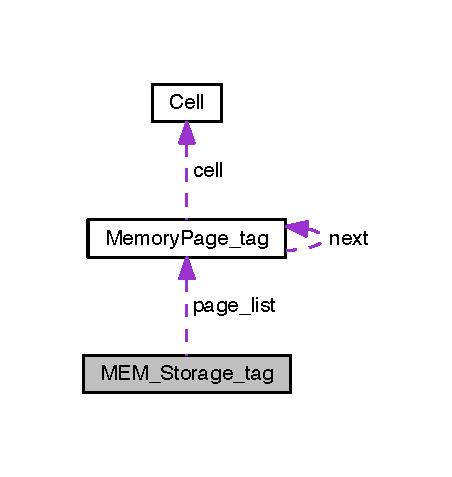
\includegraphics[width=217pt]{struct_m_e_m___storage__tag__coll__graph}
\end{center}
\end{figure}
\subsection*{Public Attributes}
\begin{DoxyCompactItemize}
\item 
\hyperlink{storage_8c_af4620055f96a48dc7cf903128aa4e665}{Memory\+Page\+List} \hyperlink{struct_m_e_m___storage__tag_a83d397628eca89e2d89a1fa6088c3b9a}{page\+\_\+list}
\item 
int \hyperlink{struct_m_e_m___storage__tag_ab81c5aee4e7f941cf9fa868e9f0ae654}{current\+\_\+page\+\_\+size}
\end{DoxyCompactItemize}


\subsection{Member Data Documentation}
\hypertarget{struct_m_e_m___storage__tag_ab81c5aee4e7f941cf9fa868e9f0ae654}{}\index{M\+E\+M\+\_\+\+Storage\+\_\+tag@{M\+E\+M\+\_\+\+Storage\+\_\+tag}!current\+\_\+page\+\_\+size@{current\+\_\+page\+\_\+size}}
\index{current\+\_\+page\+\_\+size@{current\+\_\+page\+\_\+size}!M\+E\+M\+\_\+\+Storage\+\_\+tag@{M\+E\+M\+\_\+\+Storage\+\_\+tag}}
\subsubsection[{current\+\_\+page\+\_\+size}]{\setlength{\rightskip}{0pt plus 5cm}int M\+E\+M\+\_\+\+Storage\+\_\+tag\+::current\+\_\+page\+\_\+size}\label{struct_m_e_m___storage__tag_ab81c5aee4e7f941cf9fa868e9f0ae654}
\hypertarget{struct_m_e_m___storage__tag_a83d397628eca89e2d89a1fa6088c3b9a}{}\index{M\+E\+M\+\_\+\+Storage\+\_\+tag@{M\+E\+M\+\_\+\+Storage\+\_\+tag}!page\+\_\+list@{page\+\_\+list}}
\index{page\+\_\+list@{page\+\_\+list}!M\+E\+M\+\_\+\+Storage\+\_\+tag@{M\+E\+M\+\_\+\+Storage\+\_\+tag}}
\subsubsection[{page\+\_\+list}]{\setlength{\rightskip}{0pt plus 5cm}{\bf Memory\+Page\+List} M\+E\+M\+\_\+\+Storage\+\_\+tag\+::page\+\_\+list}\label{struct_m_e_m___storage__tag_a83d397628eca89e2d89a1fa6088c3b9a}


The documentation for this struct was generated from the following file\+:\begin{DoxyCompactItemize}
\item 
memory/\hyperlink{storage_8c}{storage.\+c}\end{DoxyCompactItemize}

\hypertarget{struct_memory_page__tag}{}\section{Memory\+Page\+\_\+tag Struct Reference}
\label{struct_memory_page__tag}\index{Memory\+Page\+\_\+tag@{Memory\+Page\+\_\+tag}}


Collaboration diagram for Memory\+Page\+\_\+tag\+:\nopagebreak
\begin{figure}[H]
\begin{center}
\leavevmode
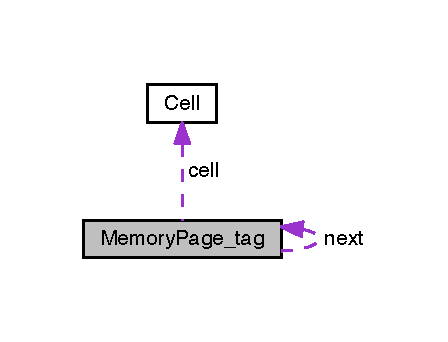
\includegraphics[width=215pt]{struct_memory_page__tag__coll__graph}
\end{center}
\end{figure}
\subsection*{Public Attributes}
\begin{DoxyCompactItemize}
\item 
int \hyperlink{struct_memory_page__tag_a683e8a1f905f2e4203bc9609c75e4e4c}{cell\+\_\+num}
\item 
int \hyperlink{struct_memory_page__tag_a21416c5c747f6617e9ecf641f086c614}{use\+\_\+cell\+\_\+num}
\item 
\hyperlink{storage_8c_af4620055f96a48dc7cf903128aa4e665}{Memory\+Page\+List} \hyperlink{struct_memory_page__tag_a53d3c92ac52441fba678eda169980229}{next}
\item 
\hyperlink{union_cell}{Cell} \hyperlink{struct_memory_page__tag_a7f1abbe528efa4a8fdea13cfc2757b8a}{cell} \mbox{[}1\mbox{]}
\end{DoxyCompactItemize}


\subsection{Member Data Documentation}
\hypertarget{struct_memory_page__tag_a7f1abbe528efa4a8fdea13cfc2757b8a}{}\index{Memory\+Page\+\_\+tag@{Memory\+Page\+\_\+tag}!cell@{cell}}
\index{cell@{cell}!Memory\+Page\+\_\+tag@{Memory\+Page\+\_\+tag}}
\subsubsection[{cell}]{\setlength{\rightskip}{0pt plus 5cm}{\bf Cell} Memory\+Page\+\_\+tag\+::cell\mbox{[}1\mbox{]}}\label{struct_memory_page__tag_a7f1abbe528efa4a8fdea13cfc2757b8a}
\hypertarget{struct_memory_page__tag_a683e8a1f905f2e4203bc9609c75e4e4c}{}\index{Memory\+Page\+\_\+tag@{Memory\+Page\+\_\+tag}!cell\+\_\+num@{cell\+\_\+num}}
\index{cell\+\_\+num@{cell\+\_\+num}!Memory\+Page\+\_\+tag@{Memory\+Page\+\_\+tag}}
\subsubsection[{cell\+\_\+num}]{\setlength{\rightskip}{0pt plus 5cm}int Memory\+Page\+\_\+tag\+::cell\+\_\+num}\label{struct_memory_page__tag_a683e8a1f905f2e4203bc9609c75e4e4c}
\hypertarget{struct_memory_page__tag_a53d3c92ac52441fba678eda169980229}{}\index{Memory\+Page\+\_\+tag@{Memory\+Page\+\_\+tag}!next@{next}}
\index{next@{next}!Memory\+Page\+\_\+tag@{Memory\+Page\+\_\+tag}}
\subsubsection[{next}]{\setlength{\rightskip}{0pt plus 5cm}{\bf Memory\+Page\+List} Memory\+Page\+\_\+tag\+::next}\label{struct_memory_page__tag_a53d3c92ac52441fba678eda169980229}
\hypertarget{struct_memory_page__tag_a21416c5c747f6617e9ecf641f086c614}{}\index{Memory\+Page\+\_\+tag@{Memory\+Page\+\_\+tag}!use\+\_\+cell\+\_\+num@{use\+\_\+cell\+\_\+num}}
\index{use\+\_\+cell\+\_\+num@{use\+\_\+cell\+\_\+num}!Memory\+Page\+\_\+tag@{Memory\+Page\+\_\+tag}}
\subsubsection[{use\+\_\+cell\+\_\+num}]{\setlength{\rightskip}{0pt plus 5cm}int Memory\+Page\+\_\+tag\+::use\+\_\+cell\+\_\+num}\label{struct_memory_page__tag_a21416c5c747f6617e9ecf641f086c614}


The documentation for this struct was generated from the following file\+:\begin{DoxyCompactItemize}
\item 
memory/\hyperlink{storage_8c}{storage.\+c}\end{DoxyCompactItemize}

\hypertarget{struct_message_argument}{}\section{Message\+Argument Struct Reference}
\label{struct_message_argument}\index{Message\+Argument@{Message\+Argument}}
\subsection*{Public Attributes}
\begin{DoxyCompactItemize}
\item 
\hyperlink{crowbar_8h_aa3bc7ab05aa3429f1f651ceabdc1be5e}{Message\+Argument\+Type} \hyperlink{struct_message_argument_ab4edae149a46b949d311508db068c999}{type}
\item 
char $\ast$ \hyperlink{struct_message_argument_afd2a134151e6db0d2f213db77cb2e36e}{name}
\item 
\begin{tabbing}
xx\=xx\=xx\=xx\=xx\=xx\=xx\=xx\=xx\=\kill
union \{\\
\>int \hyperlink{struct_message_argument_aecc4f24e519f40ff86284a2b73ef1bc8}{int\_val}\\
\>double \hyperlink{struct_message_argument_ab7f5dc20ff83d99c8556566cddc96647}{double\_val}\\
\>char $\ast$ \hyperlink{struct_message_argument_ae41f3e1492fcd9d8df1706e6e4958874}{string\_val}\\
\>void $\ast$ \hyperlink{struct_message_argument_a43017c0c8915b94ad150fbe4c1f4b02d}{pointer\_val}\\
\>int \hyperlink{struct_message_argument_a7df779277c1b7a79e117b23edecb3caa}{character\_val}\\
\} \hyperlink{struct_message_argument_a9ca164b976d87645797abcca00269976}{u}\\

\end{tabbing}\end{DoxyCompactItemize}


\subsection{Member Data Documentation}
\hypertarget{struct_message_argument_a7df779277c1b7a79e117b23edecb3caa}{}\index{Message\+Argument@{Message\+Argument}!character\+\_\+val@{character\+\_\+val}}
\index{character\+\_\+val@{character\+\_\+val}!Message\+Argument@{Message\+Argument}}
\subsubsection[{character\+\_\+val}]{\setlength{\rightskip}{0pt plus 5cm}int Message\+Argument\+::character\+\_\+val}\label{struct_message_argument_a7df779277c1b7a79e117b23edecb3caa}
\hypertarget{struct_message_argument_ab7f5dc20ff83d99c8556566cddc96647}{}\index{Message\+Argument@{Message\+Argument}!double\+\_\+val@{double\+\_\+val}}
\index{double\+\_\+val@{double\+\_\+val}!Message\+Argument@{Message\+Argument}}
\subsubsection[{double\+\_\+val}]{\setlength{\rightskip}{0pt plus 5cm}double Message\+Argument\+::double\+\_\+val}\label{struct_message_argument_ab7f5dc20ff83d99c8556566cddc96647}
\hypertarget{struct_message_argument_aecc4f24e519f40ff86284a2b73ef1bc8}{}\index{Message\+Argument@{Message\+Argument}!int\+\_\+val@{int\+\_\+val}}
\index{int\+\_\+val@{int\+\_\+val}!Message\+Argument@{Message\+Argument}}
\subsubsection[{int\+\_\+val}]{\setlength{\rightskip}{0pt plus 5cm}int Message\+Argument\+::int\+\_\+val}\label{struct_message_argument_aecc4f24e519f40ff86284a2b73ef1bc8}
\hypertarget{struct_message_argument_afd2a134151e6db0d2f213db77cb2e36e}{}\index{Message\+Argument@{Message\+Argument}!name@{name}}
\index{name@{name}!Message\+Argument@{Message\+Argument}}
\subsubsection[{name}]{\setlength{\rightskip}{0pt plus 5cm}char$\ast$ Message\+Argument\+::name}\label{struct_message_argument_afd2a134151e6db0d2f213db77cb2e36e}
\hypertarget{struct_message_argument_a43017c0c8915b94ad150fbe4c1f4b02d}{}\index{Message\+Argument@{Message\+Argument}!pointer\+\_\+val@{pointer\+\_\+val}}
\index{pointer\+\_\+val@{pointer\+\_\+val}!Message\+Argument@{Message\+Argument}}
\subsubsection[{pointer\+\_\+val}]{\setlength{\rightskip}{0pt plus 5cm}void$\ast$ Message\+Argument\+::pointer\+\_\+val}\label{struct_message_argument_a43017c0c8915b94ad150fbe4c1f4b02d}
\hypertarget{struct_message_argument_ae41f3e1492fcd9d8df1706e6e4958874}{}\index{Message\+Argument@{Message\+Argument}!string\+\_\+val@{string\+\_\+val}}
\index{string\+\_\+val@{string\+\_\+val}!Message\+Argument@{Message\+Argument}}
\subsubsection[{string\+\_\+val}]{\setlength{\rightskip}{0pt plus 5cm}char$\ast$ Message\+Argument\+::string\+\_\+val}\label{struct_message_argument_ae41f3e1492fcd9d8df1706e6e4958874}
\hypertarget{struct_message_argument_ab4edae149a46b949d311508db068c999}{}\index{Message\+Argument@{Message\+Argument}!type@{type}}
\index{type@{type}!Message\+Argument@{Message\+Argument}}
\subsubsection[{type}]{\setlength{\rightskip}{0pt plus 5cm}{\bf Message\+Argument\+Type} Message\+Argument\+::type}\label{struct_message_argument_ab4edae149a46b949d311508db068c999}
\hypertarget{struct_message_argument_a9ca164b976d87645797abcca00269976}{}\index{Message\+Argument@{Message\+Argument}!u@{u}}
\index{u@{u}!Message\+Argument@{Message\+Argument}}
\subsubsection[{u}]{\setlength{\rightskip}{0pt plus 5cm}union \{ ... \}   Message\+Argument\+::u}\label{struct_message_argument_a9ca164b976d87645797abcca00269976}


The documentation for this struct was generated from the following file\+:\begin{DoxyCompactItemize}
\item 
\hyperlink{error_8c}{error.\+c}\end{DoxyCompactItemize}

\hypertarget{struct_message_format}{}\section{Message\+Format Struct Reference}
\label{struct_message_format}\index{Message\+Format@{Message\+Format}}


{\ttfamily \#include $<$crowbar.\+h$>$}

\subsection*{Public Attributes}
\begin{DoxyCompactItemize}
\item 
char $\ast$ \hyperlink{struct_message_format_a493d7da4c1046232811f5cce284282d9}{format}
\end{DoxyCompactItemize}


\subsection{Member Data Documentation}
\hypertarget{struct_message_format_a493d7da4c1046232811f5cce284282d9}{}\index{Message\+Format@{Message\+Format}!format@{format}}
\index{format@{format}!Message\+Format@{Message\+Format}}
\subsubsection[{format}]{\setlength{\rightskip}{0pt plus 5cm}char$\ast$ Message\+Format\+::format}\label{struct_message_format_a493d7da4c1046232811f5cce284282d9}


The documentation for this struct was generated from the following file\+:\begin{DoxyCompactItemize}
\item 
\hyperlink{crowbar_8h}{crowbar.\+h}\end{DoxyCompactItemize}

\hypertarget{struct_parameter_list__tag}{}\section{Parameter\+List\+\_\+tag Struct Reference}
\label{struct_parameter_list__tag}\index{Parameter\+List\+\_\+tag@{Parameter\+List\+\_\+tag}}


{\ttfamily \#include $<$crowbar.\+h$>$}



Collaboration diagram for Parameter\+List\+\_\+tag\+:\nopagebreak
\begin{figure}[H]
\begin{center}
\leavevmode
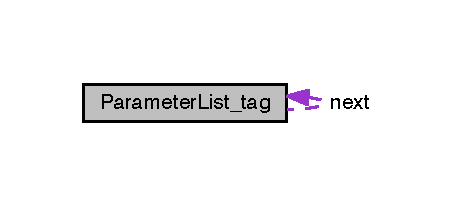
\includegraphics[width=217pt]{struct_parameter_list__tag__coll__graph}
\end{center}
\end{figure}
\subsection*{Public Attributes}
\begin{DoxyCompactItemize}
\item 
char $\ast$ \hyperlink{struct_parameter_list__tag_a704cd205e8ce6762bb2b0ac4b7d1942f}{name}
\item 
struct \hyperlink{struct_parameter_list__tag}{Parameter\+List\+\_\+tag} $\ast$ \hyperlink{struct_parameter_list__tag_a9449cbcacc0fab949f133107943d75d7}{next}
\end{DoxyCompactItemize}


\subsection{Member Data Documentation}
\hypertarget{struct_parameter_list__tag_a704cd205e8ce6762bb2b0ac4b7d1942f}{}\index{Parameter\+List\+\_\+tag@{Parameter\+List\+\_\+tag}!name@{name}}
\index{name@{name}!Parameter\+List\+\_\+tag@{Parameter\+List\+\_\+tag}}
\subsubsection[{name}]{\setlength{\rightskip}{0pt plus 5cm}char$\ast$ Parameter\+List\+\_\+tag\+::name}\label{struct_parameter_list__tag_a704cd205e8ce6762bb2b0ac4b7d1942f}
\hypertarget{struct_parameter_list__tag_a9449cbcacc0fab949f133107943d75d7}{}\index{Parameter\+List\+\_\+tag@{Parameter\+List\+\_\+tag}!next@{next}}
\index{next@{next}!Parameter\+List\+\_\+tag@{Parameter\+List\+\_\+tag}}
\subsubsection[{next}]{\setlength{\rightskip}{0pt plus 5cm}struct {\bf Parameter\+List\+\_\+tag}$\ast$ Parameter\+List\+\_\+tag\+::next}\label{struct_parameter_list__tag_a9449cbcacc0fab949f133107943d75d7}


The documentation for this struct was generated from the following file\+:\begin{DoxyCompactItemize}
\item 
\hyperlink{crowbar_8h}{crowbar.\+h}\end{DoxyCompactItemize}

\hypertarget{struct_return_statement}{}\section{Return\+Statement Struct Reference}
\label{struct_return_statement}\index{Return\+Statement@{Return\+Statement}}


{\ttfamily \#include $<$crowbar.\+h$>$}



Collaboration diagram for Return\+Statement\+:\nopagebreak
\begin{figure}[H]
\begin{center}
\leavevmode
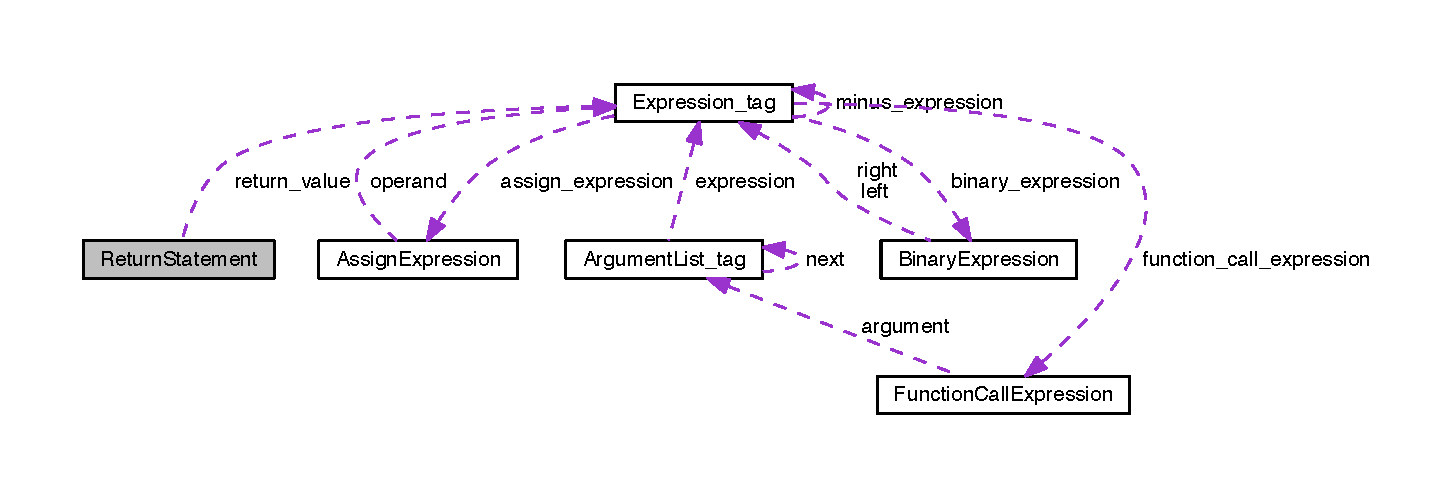
\includegraphics[width=350pt]{struct_return_statement__coll__graph}
\end{center}
\end{figure}
\subsection*{Public Attributes}
\begin{DoxyCompactItemize}
\item 
\hyperlink{crowbar_8h_a070c6feb370aad8a9665ca315bf6ed4a}{Expression} $\ast$ \hyperlink{struct_return_statement_ae0abf27e1b4dc529fdd363d80b640b88}{return\+\_\+value}
\end{DoxyCompactItemize}


\subsection{Member Data Documentation}
\hypertarget{struct_return_statement_ae0abf27e1b4dc529fdd363d80b640b88}{}\index{Return\+Statement@{Return\+Statement}!return\+\_\+value@{return\+\_\+value}}
\index{return\+\_\+value@{return\+\_\+value}!Return\+Statement@{Return\+Statement}}
\subsubsection[{return\+\_\+value}]{\setlength{\rightskip}{0pt plus 5cm}{\bf Expression}$\ast$ Return\+Statement\+::return\+\_\+value}\label{struct_return_statement_ae0abf27e1b4dc529fdd363d80b640b88}


The documentation for this struct was generated from the following file\+:\begin{DoxyCompactItemize}
\item 
\hyperlink{crowbar_8h}{crowbar.\+h}\end{DoxyCompactItemize}

\hypertarget{struct_statement__tag}{}\section{Statement\+\_\+tag Struct Reference}
\label{struct_statement__tag}\index{Statement\+\_\+tag@{Statement\+\_\+tag}}


{\ttfamily \#include $<$crowbar.\+h$>$}



Collaboration diagram for Statement\+\_\+tag\+:\nopagebreak
\begin{figure}[H]
\begin{center}
\leavevmode
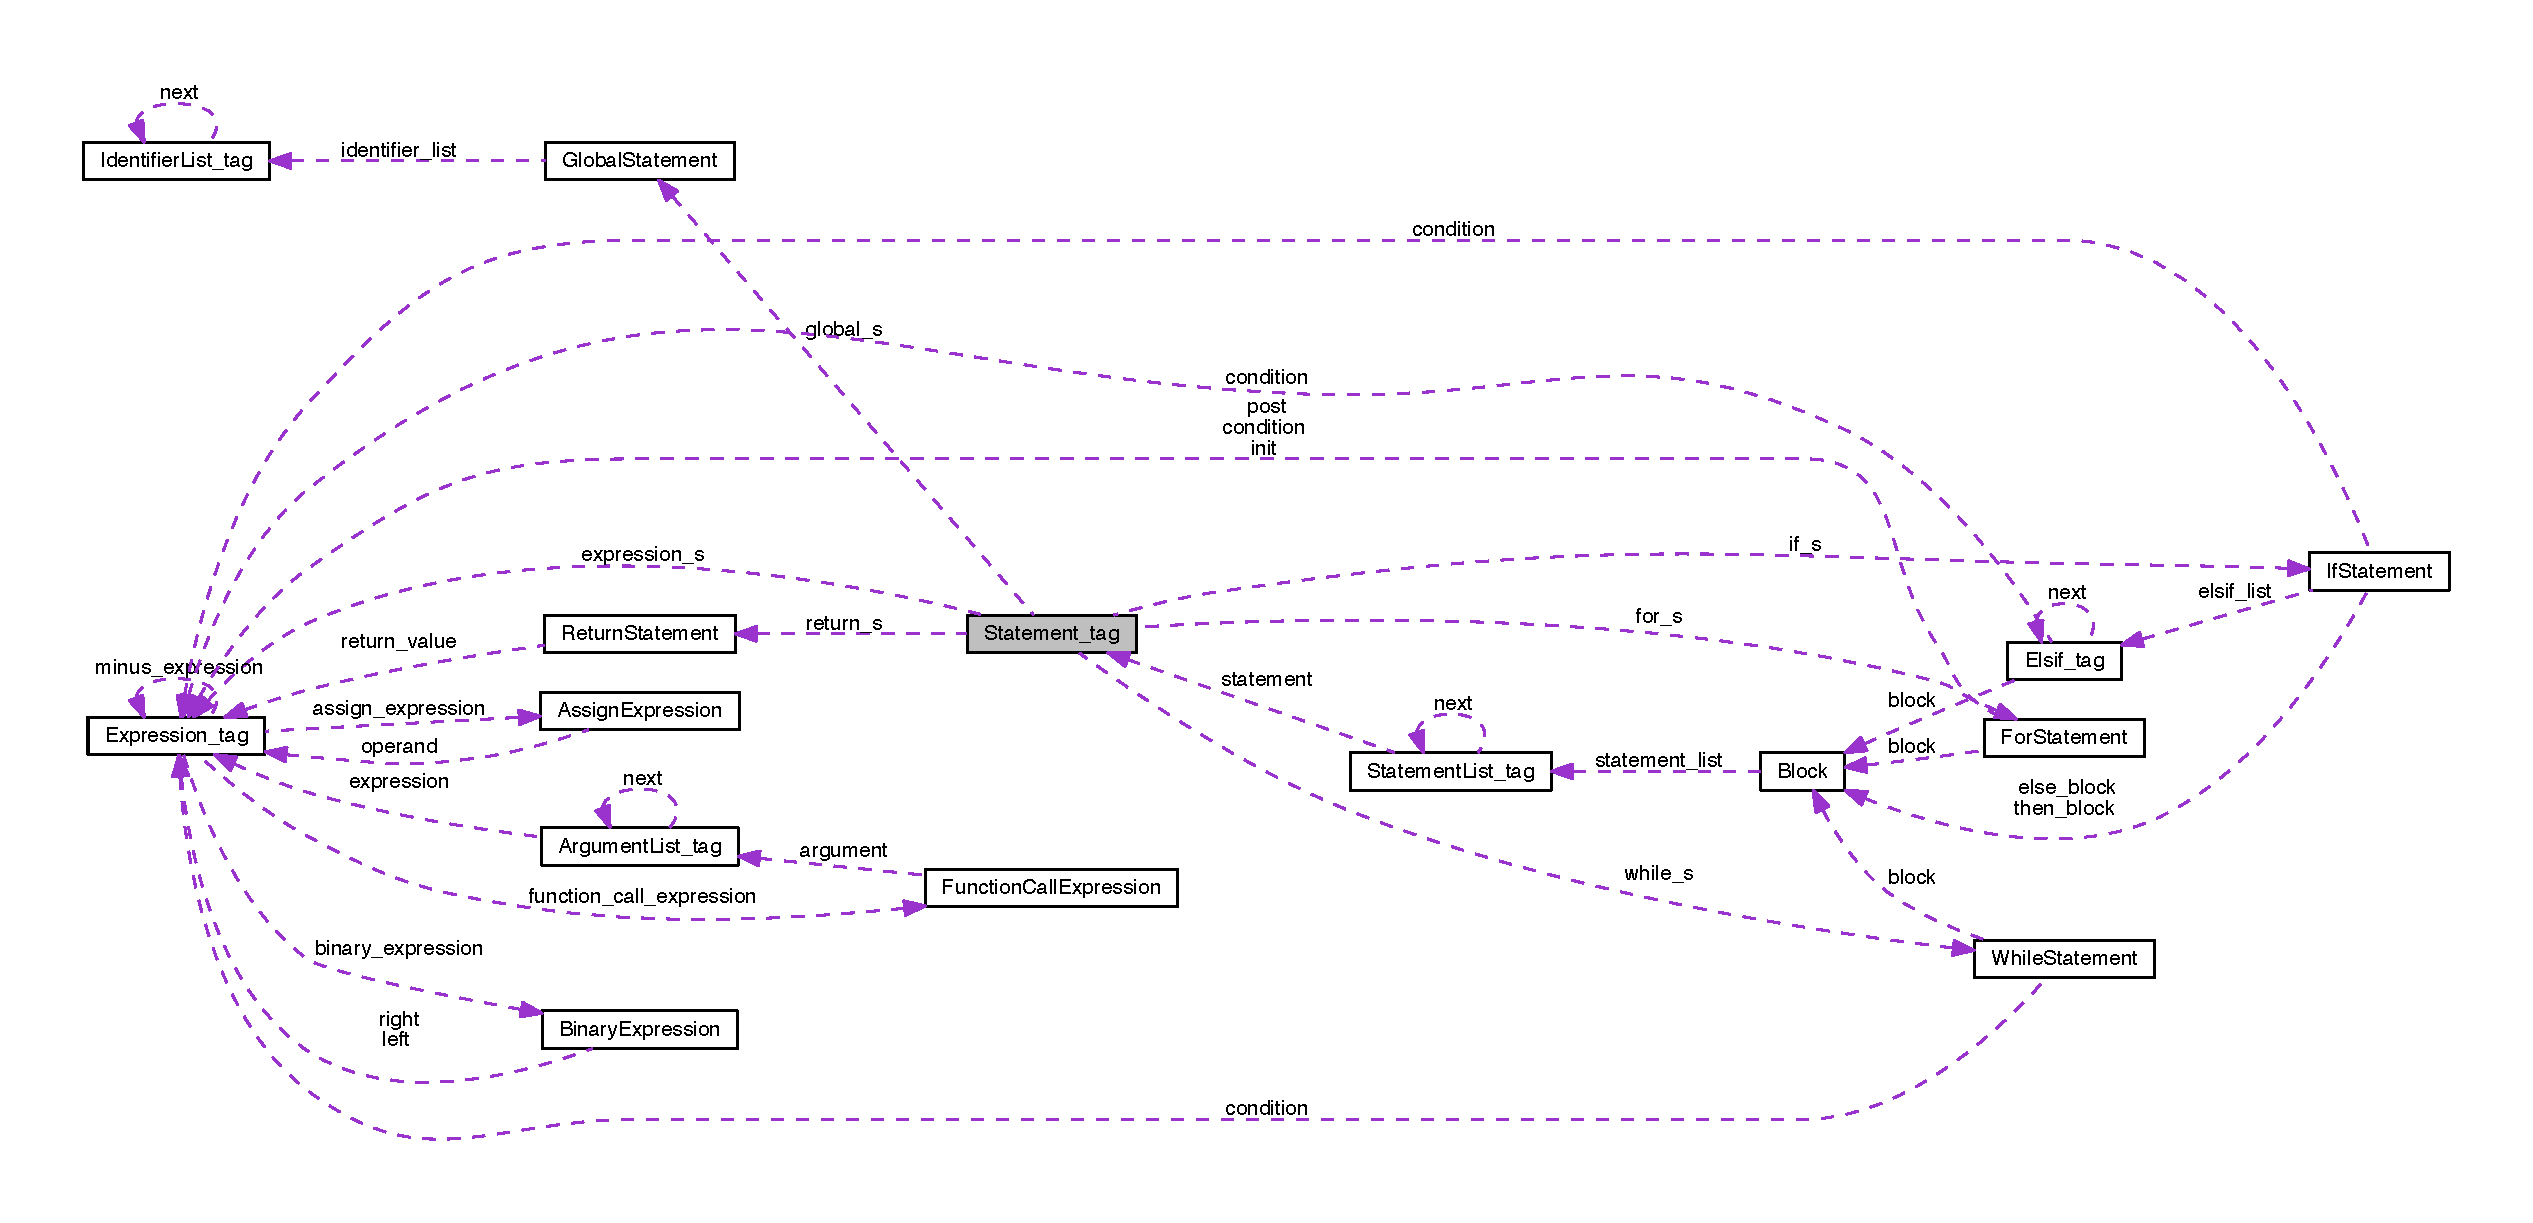
\includegraphics[width=350pt]{struct_statement__tag__coll__graph}
\end{center}
\end{figure}
\subsection*{Public Attributes}
\begin{DoxyCompactItemize}
\item 
\hyperlink{crowbar_8h_a5f5d0dfd807d2356ecc3cdabf71b3d53}{Statement\+Type} \hyperlink{struct_statement__tag_abe1b2488e3a8c4277078f8c1b7c86482}{type}
\item 
int \hyperlink{struct_statement__tag_a96dcb197dafe54cf45fcf2d5123f7ab3}{line\+\_\+number}
\item 
\begin{tabbing}
xx\=xx\=xx\=xx\=xx\=xx\=xx\=xx\=xx\=\kill
union \{\\
\>\hyperlink{crowbar_8h_a070c6feb370aad8a9665ca315bf6ed4a}{Expression} $\ast$ \hyperlink{struct_statement__tag_abb838fa3163c91f43a36d1ba87674c87}{expression\_s}\\
\>\hyperlink{struct_global_statement}{GlobalStatement} \hyperlink{struct_statement__tag_a0a05cf3ddbe6aa28a52c97cb17aebc53}{global\_s}\\
\>\hyperlink{struct_if_statement}{IfStatement} \hyperlink{struct_statement__tag_a0e4d01f350eb7ea2e195c82638d38ec4}{if\_s}\\
\>\hyperlink{struct_while_statement}{WhileStatement} \hyperlink{struct_statement__tag_ad897c318f35e7476a81dcf1eb2275f89}{while\_s}\\
\>\hyperlink{struct_for_statement}{ForStatement} \hyperlink{struct_statement__tag_a3299f7bafe47d4b9a2ab4a23f30de671}{for\_s}\\
\>\hyperlink{struct_return_statement}{ReturnStatement} \hyperlink{struct_statement__tag_afe3a97a689d2ac59f84600f220cdad1e}{return\_s}\\
\} \hyperlink{struct_statement__tag_a33748df145380d0099e0941d3c937265}{u}\\

\end{tabbing}\end{DoxyCompactItemize}


\subsection{Member Data Documentation}
\hypertarget{struct_statement__tag_abb838fa3163c91f43a36d1ba87674c87}{}\index{Statement\+\_\+tag@{Statement\+\_\+tag}!expression\+\_\+s@{expression\+\_\+s}}
\index{expression\+\_\+s@{expression\+\_\+s}!Statement\+\_\+tag@{Statement\+\_\+tag}}
\subsubsection[{expression\+\_\+s}]{\setlength{\rightskip}{0pt plus 5cm}{\bf Expression}$\ast$ Statement\+\_\+tag\+::expression\+\_\+s}\label{struct_statement__tag_abb838fa3163c91f43a36d1ba87674c87}
\hypertarget{struct_statement__tag_a3299f7bafe47d4b9a2ab4a23f30de671}{}\index{Statement\+\_\+tag@{Statement\+\_\+tag}!for\+\_\+s@{for\+\_\+s}}
\index{for\+\_\+s@{for\+\_\+s}!Statement\+\_\+tag@{Statement\+\_\+tag}}
\subsubsection[{for\+\_\+s}]{\setlength{\rightskip}{0pt plus 5cm}{\bf For\+Statement} Statement\+\_\+tag\+::for\+\_\+s}\label{struct_statement__tag_a3299f7bafe47d4b9a2ab4a23f30de671}
\hypertarget{struct_statement__tag_a0a05cf3ddbe6aa28a52c97cb17aebc53}{}\index{Statement\+\_\+tag@{Statement\+\_\+tag}!global\+\_\+s@{global\+\_\+s}}
\index{global\+\_\+s@{global\+\_\+s}!Statement\+\_\+tag@{Statement\+\_\+tag}}
\subsubsection[{global\+\_\+s}]{\setlength{\rightskip}{0pt plus 5cm}{\bf Global\+Statement} Statement\+\_\+tag\+::global\+\_\+s}\label{struct_statement__tag_a0a05cf3ddbe6aa28a52c97cb17aebc53}
\hypertarget{struct_statement__tag_a0e4d01f350eb7ea2e195c82638d38ec4}{}\index{Statement\+\_\+tag@{Statement\+\_\+tag}!if\+\_\+s@{if\+\_\+s}}
\index{if\+\_\+s@{if\+\_\+s}!Statement\+\_\+tag@{Statement\+\_\+tag}}
\subsubsection[{if\+\_\+s}]{\setlength{\rightskip}{0pt plus 5cm}{\bf If\+Statement} Statement\+\_\+tag\+::if\+\_\+s}\label{struct_statement__tag_a0e4d01f350eb7ea2e195c82638d38ec4}
\hypertarget{struct_statement__tag_a96dcb197dafe54cf45fcf2d5123f7ab3}{}\index{Statement\+\_\+tag@{Statement\+\_\+tag}!line\+\_\+number@{line\+\_\+number}}
\index{line\+\_\+number@{line\+\_\+number}!Statement\+\_\+tag@{Statement\+\_\+tag}}
\subsubsection[{line\+\_\+number}]{\setlength{\rightskip}{0pt plus 5cm}int Statement\+\_\+tag\+::line\+\_\+number}\label{struct_statement__tag_a96dcb197dafe54cf45fcf2d5123f7ab3}
\hypertarget{struct_statement__tag_afe3a97a689d2ac59f84600f220cdad1e}{}\index{Statement\+\_\+tag@{Statement\+\_\+tag}!return\+\_\+s@{return\+\_\+s}}
\index{return\+\_\+s@{return\+\_\+s}!Statement\+\_\+tag@{Statement\+\_\+tag}}
\subsubsection[{return\+\_\+s}]{\setlength{\rightskip}{0pt plus 5cm}{\bf Return\+Statement} Statement\+\_\+tag\+::return\+\_\+s}\label{struct_statement__tag_afe3a97a689d2ac59f84600f220cdad1e}
\hypertarget{struct_statement__tag_abe1b2488e3a8c4277078f8c1b7c86482}{}\index{Statement\+\_\+tag@{Statement\+\_\+tag}!type@{type}}
\index{type@{type}!Statement\+\_\+tag@{Statement\+\_\+tag}}
\subsubsection[{type}]{\setlength{\rightskip}{0pt plus 5cm}{\bf Statement\+Type} Statement\+\_\+tag\+::type}\label{struct_statement__tag_abe1b2488e3a8c4277078f8c1b7c86482}
\hypertarget{struct_statement__tag_a33748df145380d0099e0941d3c937265}{}\index{Statement\+\_\+tag@{Statement\+\_\+tag}!u@{u}}
\index{u@{u}!Statement\+\_\+tag@{Statement\+\_\+tag}}
\subsubsection[{u}]{\setlength{\rightskip}{0pt plus 5cm}union \{ ... \}   Statement\+\_\+tag\+::u}\label{struct_statement__tag_a33748df145380d0099e0941d3c937265}
\hypertarget{struct_statement__tag_ad897c318f35e7476a81dcf1eb2275f89}{}\index{Statement\+\_\+tag@{Statement\+\_\+tag}!while\+\_\+s@{while\+\_\+s}}
\index{while\+\_\+s@{while\+\_\+s}!Statement\+\_\+tag@{Statement\+\_\+tag}}
\subsubsection[{while\+\_\+s}]{\setlength{\rightskip}{0pt plus 5cm}{\bf While\+Statement} Statement\+\_\+tag\+::while\+\_\+s}\label{struct_statement__tag_ad897c318f35e7476a81dcf1eb2275f89}


The documentation for this struct was generated from the following file\+:\begin{DoxyCompactItemize}
\item 
\hyperlink{crowbar_8h}{crowbar.\+h}\end{DoxyCompactItemize}

\hypertarget{struct_statement_list__tag}{}\section{Statement\+List\+\_\+tag Struct Reference}
\label{struct_statement_list__tag}\index{Statement\+List\+\_\+tag@{Statement\+List\+\_\+tag}}


{\ttfamily \#include $<$crowbar.\+h$>$}



Collaboration diagram for Statement\+List\+\_\+tag\+:\nopagebreak
\begin{figure}[H]
\begin{center}
\leavevmode
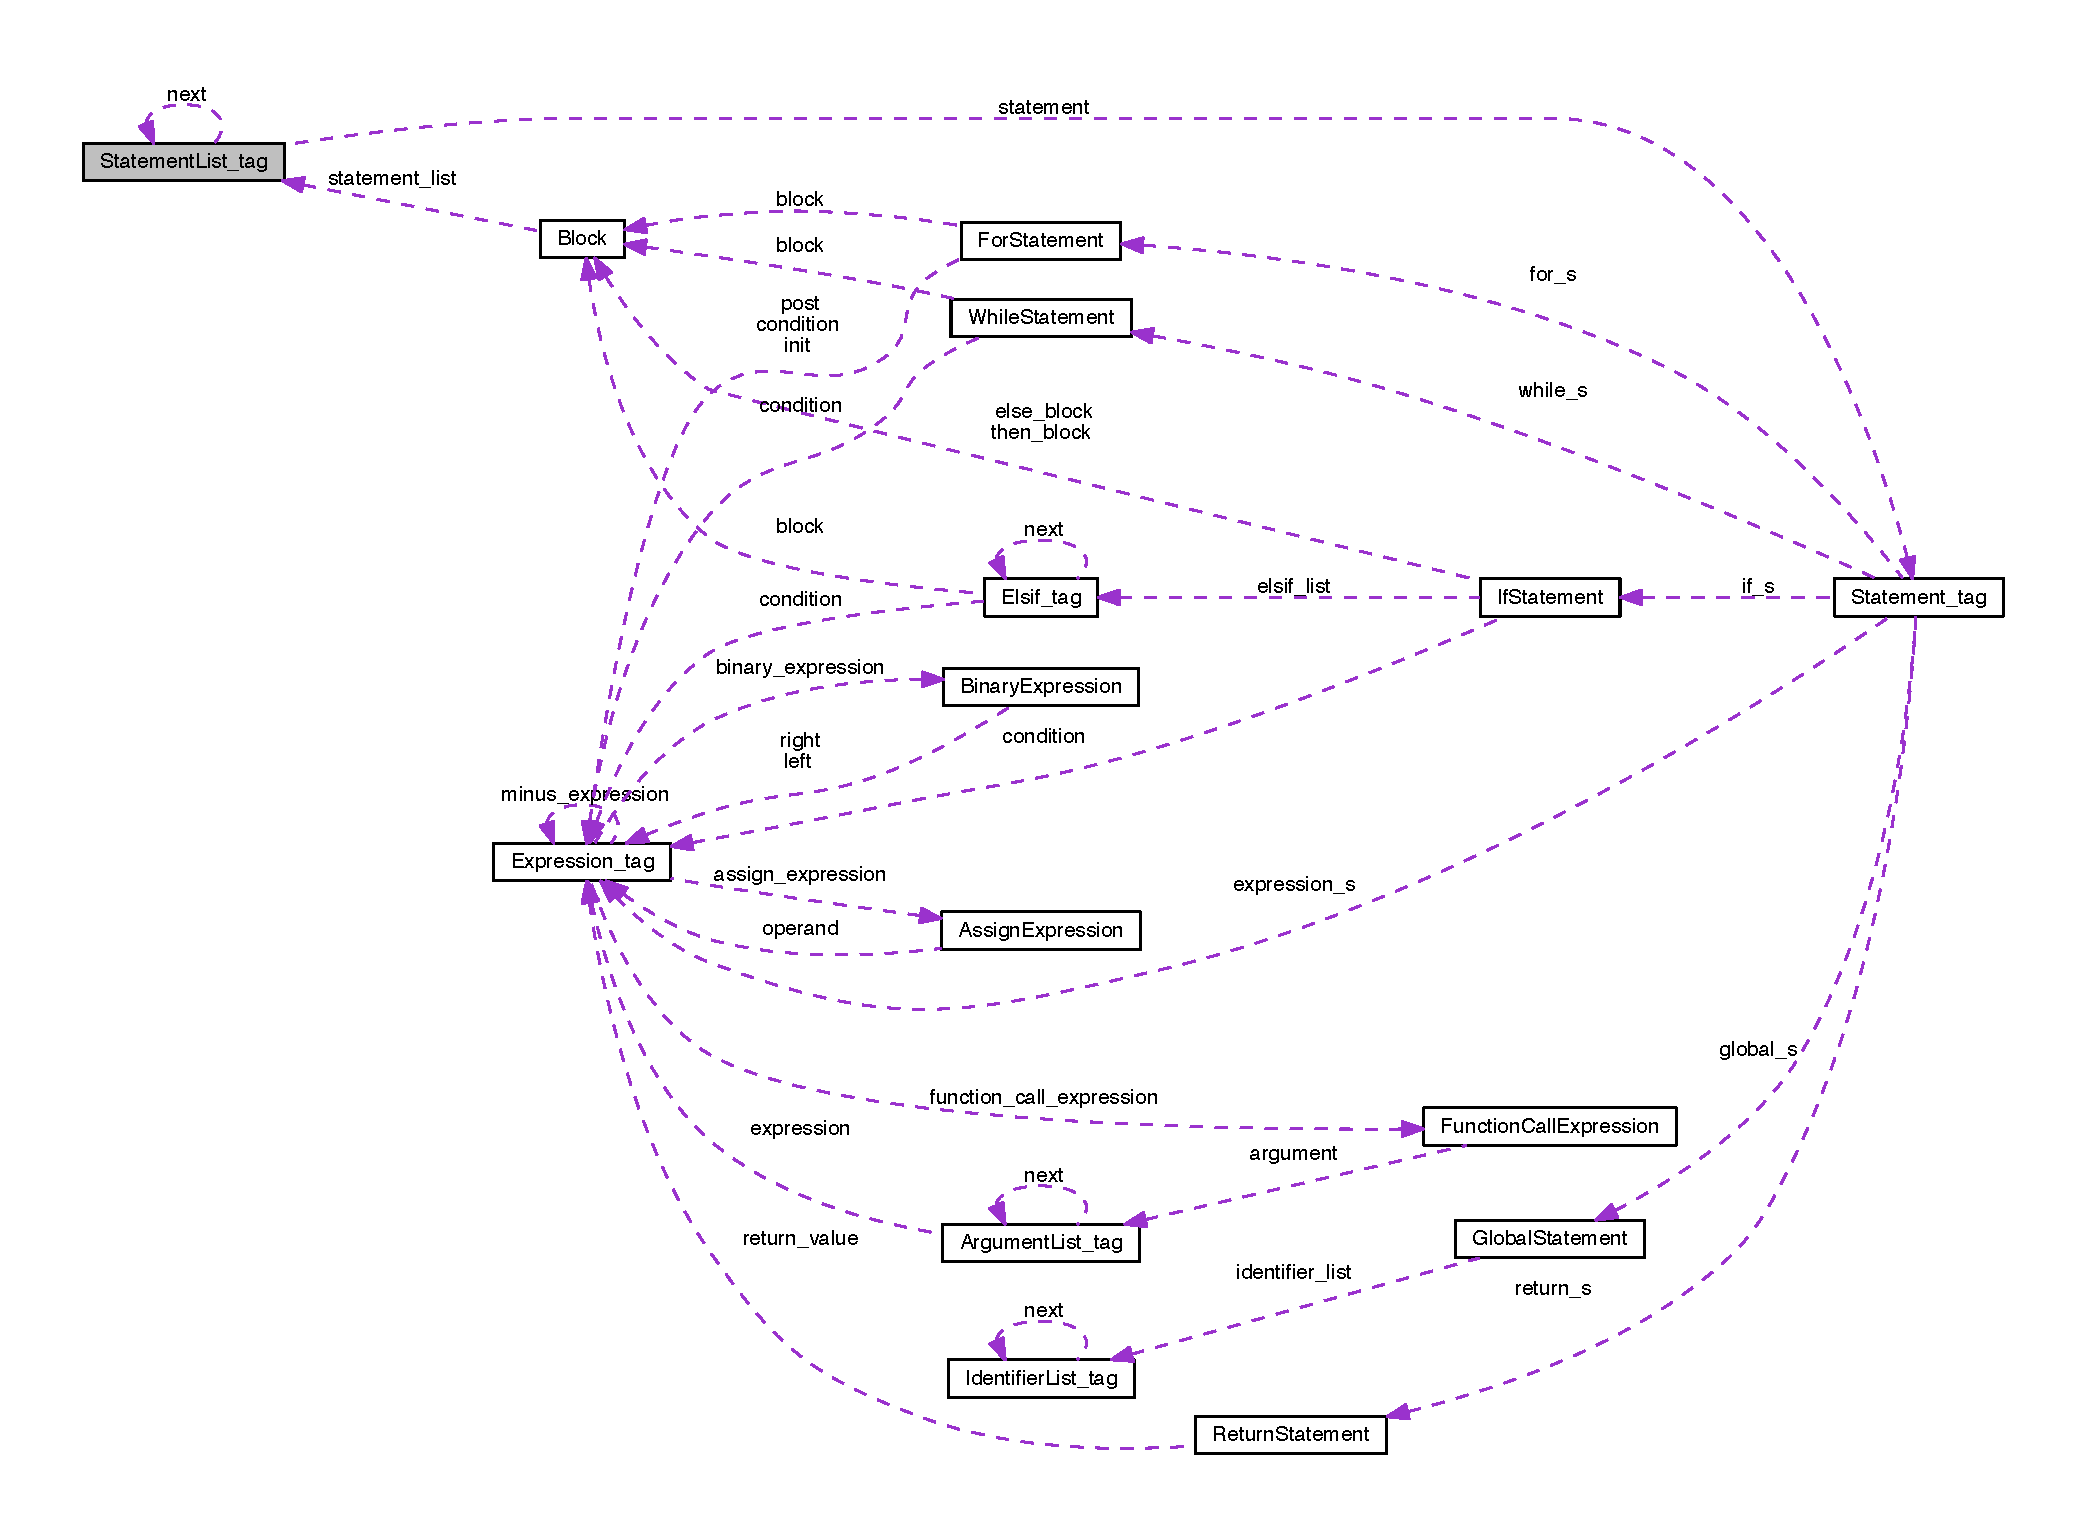
\includegraphics[width=350pt]{struct_statement_list__tag__coll__graph}
\end{center}
\end{figure}
\subsection*{Public Attributes}
\begin{DoxyCompactItemize}
\item 
\hyperlink{crowbar_8h_a16fe74a7a87df7652e815d139b3349d2}{Statement} $\ast$ \hyperlink{struct_statement_list__tag_af8e00b3cdbd4364e5c5c23896df4697d}{statement}
\item 
struct \hyperlink{struct_statement_list__tag}{Statement\+List\+\_\+tag} $\ast$ \hyperlink{struct_statement_list__tag_a1e3b82b453a9f9d654c0d6b5313009be}{next}
\end{DoxyCompactItemize}


\subsection{Member Data Documentation}
\hypertarget{struct_statement_list__tag_a1e3b82b453a9f9d654c0d6b5313009be}{}\index{Statement\+List\+\_\+tag@{Statement\+List\+\_\+tag}!next@{next}}
\index{next@{next}!Statement\+List\+\_\+tag@{Statement\+List\+\_\+tag}}
\subsubsection[{next}]{\setlength{\rightskip}{0pt plus 5cm}struct {\bf Statement\+List\+\_\+tag}$\ast$ Statement\+List\+\_\+tag\+::next}\label{struct_statement_list__tag_a1e3b82b453a9f9d654c0d6b5313009be}
\hypertarget{struct_statement_list__tag_af8e00b3cdbd4364e5c5c23896df4697d}{}\index{Statement\+List\+\_\+tag@{Statement\+List\+\_\+tag}!statement@{statement}}
\index{statement@{statement}!Statement\+List\+\_\+tag@{Statement\+List\+\_\+tag}}
\subsubsection[{statement}]{\setlength{\rightskip}{0pt plus 5cm}{\bf Statement}$\ast$ Statement\+List\+\_\+tag\+::statement}\label{struct_statement_list__tag_af8e00b3cdbd4364e5c5c23896df4697d}


The documentation for this struct was generated from the following file\+:\begin{DoxyCompactItemize}
\item 
\hyperlink{crowbar_8h}{crowbar.\+h}\end{DoxyCompactItemize}

\hypertarget{struct_statement_result}{}\section{Statement\+Result Struct Reference}
\label{struct_statement_result}\index{Statement\+Result@{Statement\+Result}}


{\ttfamily \#include $<$crowbar.\+h$>$}



Collaboration diagram for Statement\+Result\+:\nopagebreak
\begin{figure}[H]
\begin{center}
\leavevmode
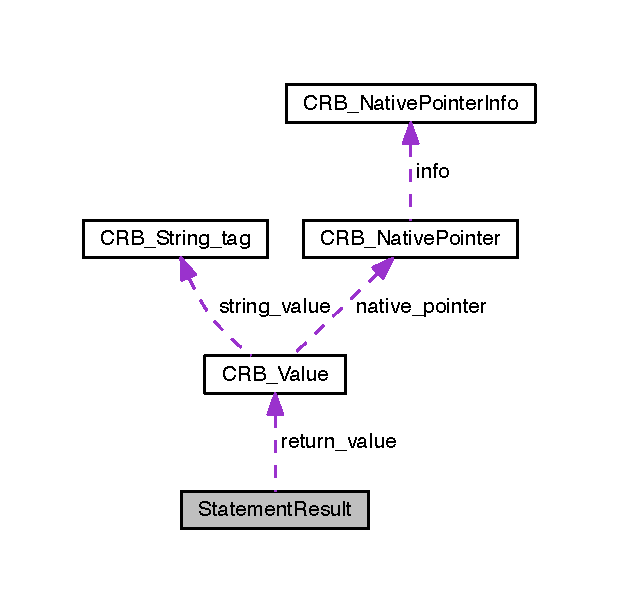
\includegraphics[width=297pt]{struct_statement_result__coll__graph}
\end{center}
\end{figure}
\subsection*{Public Attributes}
\begin{DoxyCompactItemize}
\item 
\hyperlink{crowbar_8h_afba1fe14e53276aeab17faf3818e77c1}{Statement\+Result\+Type} \hyperlink{struct_statement_result_a1c65be71416a40eea23153d5af3f7d19}{type}
\item 
\begin{tabbing}
xx\=xx\=xx\=xx\=xx\=xx\=xx\=xx\=xx\=\kill
union \{\\
\>\hyperlink{struct_c_r_b___value}{CRB\_Value} \hyperlink{struct_statement_result_a83ca729f73987f1358be29ca21c2349e}{return\_value}\\
\} \hyperlink{struct_statement_result_a3922b8f85edf104dbe464831804f9816}{u}\\

\end{tabbing}\end{DoxyCompactItemize}


\subsection{Member Data Documentation}
\hypertarget{struct_statement_result_a83ca729f73987f1358be29ca21c2349e}{}\index{Statement\+Result@{Statement\+Result}!return\+\_\+value@{return\+\_\+value}}
\index{return\+\_\+value@{return\+\_\+value}!Statement\+Result@{Statement\+Result}}
\subsubsection[{return\+\_\+value}]{\setlength{\rightskip}{0pt plus 5cm}{\bf C\+R\+B\+\_\+\+Value} Statement\+Result\+::return\+\_\+value}\label{struct_statement_result_a83ca729f73987f1358be29ca21c2349e}
\hypertarget{struct_statement_result_a1c65be71416a40eea23153d5af3f7d19}{}\index{Statement\+Result@{Statement\+Result}!type@{type}}
\index{type@{type}!Statement\+Result@{Statement\+Result}}
\subsubsection[{type}]{\setlength{\rightskip}{0pt plus 5cm}{\bf Statement\+Result\+Type} Statement\+Result\+::type}\label{struct_statement_result_a1c65be71416a40eea23153d5af3f7d19}
\hypertarget{struct_statement_result_a3922b8f85edf104dbe464831804f9816}{}\index{Statement\+Result@{Statement\+Result}!u@{u}}
\index{u@{u}!Statement\+Result@{Statement\+Result}}
\subsubsection[{u}]{\setlength{\rightskip}{0pt plus 5cm}union \{ ... \}   Statement\+Result\+::u}\label{struct_statement_result_a3922b8f85edf104dbe464831804f9816}


The documentation for this struct was generated from the following file\+:\begin{DoxyCompactItemize}
\item 
\hyperlink{crowbar_8h}{crowbar.\+h}\end{DoxyCompactItemize}

\hypertarget{struct_string_pool}{}\section{String\+Pool Struct Reference}
\label{struct_string_pool}\index{String\+Pool@{String\+Pool}}


{\ttfamily \#include $<$crowbar.\+h$>$}



Collaboration diagram for String\+Pool\+:\nopagebreak
\begin{figure}[H]
\begin{center}
\leavevmode
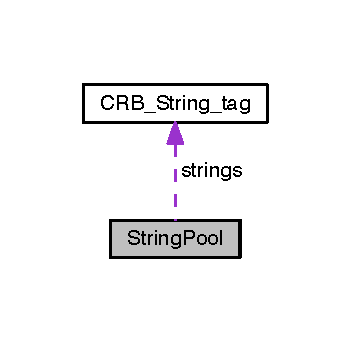
\includegraphics[width=168pt]{struct_string_pool__coll__graph}
\end{center}
\end{figure}
\subsection*{Public Attributes}
\begin{DoxyCompactItemize}
\item 
\hyperlink{_c_r_b__dev_8h_a0372b51b327f3425e983d9924fc713f8}{C\+R\+B\+\_\+\+String} $\ast$ \hyperlink{struct_string_pool_ac05ee15c6ce0fce010b86c2e25ca814e}{strings}
\end{DoxyCompactItemize}


\subsection{Member Data Documentation}
\hypertarget{struct_string_pool_ac05ee15c6ce0fce010b86c2e25ca814e}{}\index{String\+Pool@{String\+Pool}!strings@{strings}}
\index{strings@{strings}!String\+Pool@{String\+Pool}}
\subsubsection[{strings}]{\setlength{\rightskip}{0pt plus 5cm}{\bf C\+R\+B\+\_\+\+String}$\ast$ String\+Pool\+::strings}\label{struct_string_pool_ac05ee15c6ce0fce010b86c2e25ca814e}


The documentation for this struct was generated from the following file\+:\begin{DoxyCompactItemize}
\item 
\hyperlink{crowbar_8h}{crowbar.\+h}\end{DoxyCompactItemize}

\hypertarget{struct_variable__tag}{}\section{Variable\+\_\+tag Struct Reference}
\label{struct_variable__tag}\index{Variable\+\_\+tag@{Variable\+\_\+tag}}


{\ttfamily \#include $<$crowbar.\+h$>$}



Collaboration diagram for Variable\+\_\+tag\+:\nopagebreak
\begin{figure}[H]
\begin{center}
\leavevmode
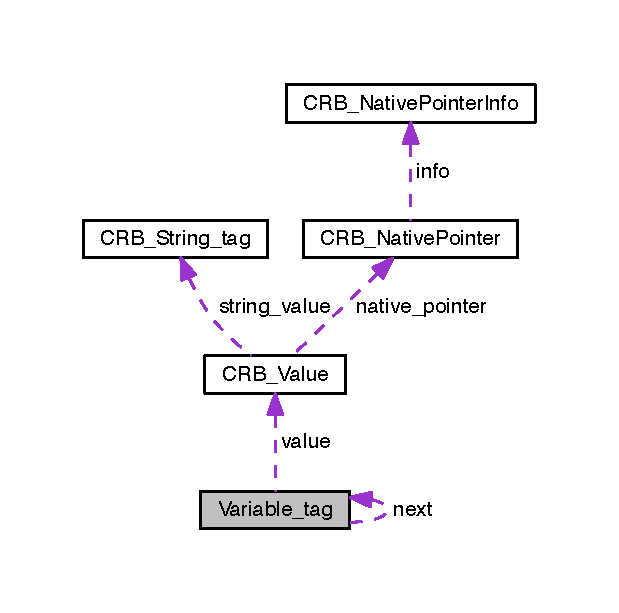
\includegraphics[width=297pt]{struct_variable__tag__coll__graph}
\end{center}
\end{figure}
\subsection*{Public Attributes}
\begin{DoxyCompactItemize}
\item 
char $\ast$ \hyperlink{struct_variable__tag_a1af2d16a129d37300d04c8a182e73d2b}{name}
\item 
\hyperlink{struct_c_r_b___value}{C\+R\+B\+\_\+\+Value} \hyperlink{struct_variable__tag_a28da53976be439d10306ef7de2869cd9}{value}
\item 
struct \hyperlink{struct_variable__tag}{Variable\+\_\+tag} $\ast$ \hyperlink{struct_variable__tag_ae8081b0ed51372eaf9b8df2bb669f7a5}{next}
\end{DoxyCompactItemize}


\subsection{Member Data Documentation}
\hypertarget{struct_variable__tag_a1af2d16a129d37300d04c8a182e73d2b}{}\index{Variable\+\_\+tag@{Variable\+\_\+tag}!name@{name}}
\index{name@{name}!Variable\+\_\+tag@{Variable\+\_\+tag}}
\subsubsection[{name}]{\setlength{\rightskip}{0pt plus 5cm}char$\ast$ Variable\+\_\+tag\+::name}\label{struct_variable__tag_a1af2d16a129d37300d04c8a182e73d2b}
\hypertarget{struct_variable__tag_ae8081b0ed51372eaf9b8df2bb669f7a5}{}\index{Variable\+\_\+tag@{Variable\+\_\+tag}!next@{next}}
\index{next@{next}!Variable\+\_\+tag@{Variable\+\_\+tag}}
\subsubsection[{next}]{\setlength{\rightskip}{0pt plus 5cm}struct {\bf Variable\+\_\+tag}$\ast$ Variable\+\_\+tag\+::next}\label{struct_variable__tag_ae8081b0ed51372eaf9b8df2bb669f7a5}
\hypertarget{struct_variable__tag_a28da53976be439d10306ef7de2869cd9}{}\index{Variable\+\_\+tag@{Variable\+\_\+tag}!value@{value}}
\index{value@{value}!Variable\+\_\+tag@{Variable\+\_\+tag}}
\subsubsection[{value}]{\setlength{\rightskip}{0pt plus 5cm}{\bf C\+R\+B\+\_\+\+Value} Variable\+\_\+tag\+::value}\label{struct_variable__tag_a28da53976be439d10306ef7de2869cd9}


The documentation for this struct was generated from the following file\+:\begin{DoxyCompactItemize}
\item 
\hyperlink{crowbar_8h}{crowbar.\+h}\end{DoxyCompactItemize}

\hypertarget{struct_v_string}{}\section{V\+String Struct Reference}
\label{struct_v_string}\index{V\+String@{V\+String}}
\subsection*{Public Attributes}
\begin{DoxyCompactItemize}
\item 
char $\ast$ \hyperlink{struct_v_string_a5c80f4b8543aaaf94e4be6c2e7d422a5}{string}
\end{DoxyCompactItemize}


\subsection{Member Data Documentation}
\hypertarget{struct_v_string_a5c80f4b8543aaaf94e4be6c2e7d422a5}{}\index{V\+String@{V\+String}!string@{string}}
\index{string@{string}!V\+String@{V\+String}}
\subsubsection[{string}]{\setlength{\rightskip}{0pt plus 5cm}char$\ast$ V\+String\+::string}\label{struct_v_string_a5c80f4b8543aaaf94e4be6c2e7d422a5}


The documentation for this struct was generated from the following file\+:\begin{DoxyCompactItemize}
\item 
\hyperlink{error_8c}{error.\+c}\end{DoxyCompactItemize}

\hypertarget{struct_while_statement}{}\section{While\+Statement Struct Reference}
\label{struct_while_statement}\index{While\+Statement@{While\+Statement}}


{\ttfamily \#include $<$crowbar.\+h$>$}



Collaboration diagram for While\+Statement\+:\nopagebreak
\begin{figure}[H]
\begin{center}
\leavevmode
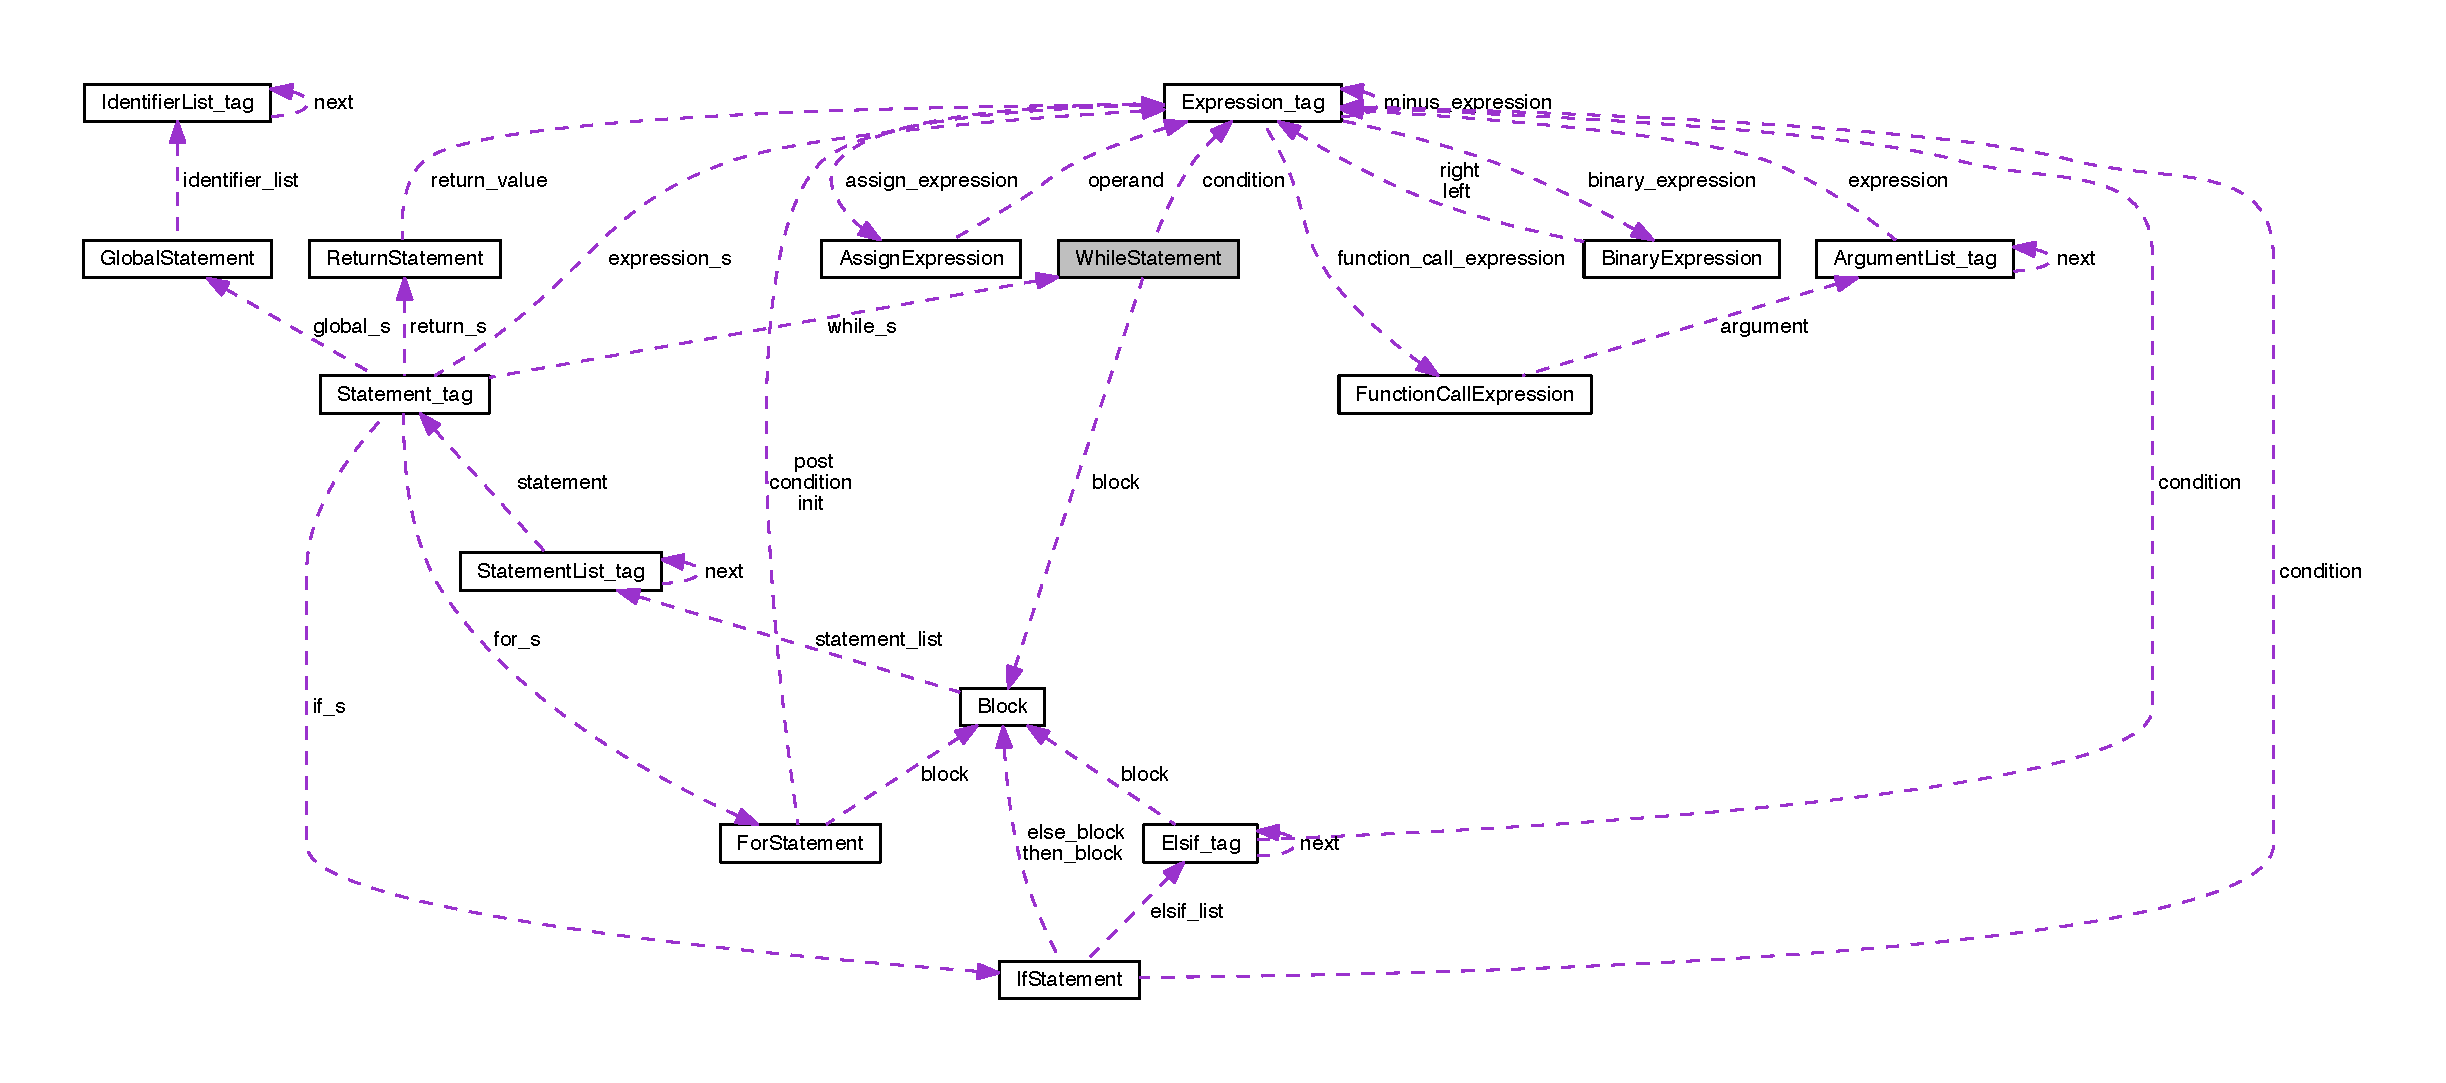
\includegraphics[width=350pt]{struct_while_statement__coll__graph}
\end{center}
\end{figure}
\subsection*{Public Attributes}
\begin{DoxyCompactItemize}
\item 
\hyperlink{crowbar_8h_a070c6feb370aad8a9665ca315bf6ed4a}{Expression} $\ast$ \hyperlink{struct_while_statement_af0f54d7883033e8be83f790afefbae75}{condition}
\item 
\hyperlink{struct_block}{Block} $\ast$ \hyperlink{struct_while_statement_a3cb552a56e39942279e23c2d75df37f4}{block}
\end{DoxyCompactItemize}


\subsection{Member Data Documentation}
\hypertarget{struct_while_statement_a3cb552a56e39942279e23c2d75df37f4}{}\index{While\+Statement@{While\+Statement}!block@{block}}
\index{block@{block}!While\+Statement@{While\+Statement}}
\subsubsection[{block}]{\setlength{\rightskip}{0pt plus 5cm}{\bf Block}$\ast$ While\+Statement\+::block}\label{struct_while_statement_a3cb552a56e39942279e23c2d75df37f4}
\hypertarget{struct_while_statement_af0f54d7883033e8be83f790afefbae75}{}\index{While\+Statement@{While\+Statement}!condition@{condition}}
\index{condition@{condition}!While\+Statement@{While\+Statement}}
\subsubsection[{condition}]{\setlength{\rightskip}{0pt plus 5cm}{\bf Expression}$\ast$ While\+Statement\+::condition}\label{struct_while_statement_af0f54d7883033e8be83f790afefbae75}


The documentation for this struct was generated from the following file\+:\begin{DoxyCompactItemize}
\item 
\hyperlink{crowbar_8h}{crowbar.\+h}\end{DoxyCompactItemize}

\hypertarget{structyy__buffer__state}{}\section{yy\+\_\+buffer\+\_\+state Struct Reference}
\label{structyy__buffer__state}\index{yy\+\_\+buffer\+\_\+state@{yy\+\_\+buffer\+\_\+state}}
\subsection*{Public Attributes}
\begin{DoxyCompactItemize}
\item 
F\+I\+L\+E $\ast$ \hyperlink{structyy__buffer__state_a4843d1422e3276b636d475a3095bd948}{yy\+\_\+input\+\_\+file}
\item 
char $\ast$ \hyperlink{structyy__buffer__state_ad7b8df8d8a4688e57b0b8d3ca75adc85}{yy\+\_\+ch\+\_\+buf}
\item 
char $\ast$ \hyperlink{structyy__buffer__state_a58aa927f098b99d99e75da80f9b681ef}{yy\+\_\+buf\+\_\+pos}
\item 
\hyperlink{lex_8yy_8c_ad557845057f187eec4be07e2717d2afa}{yy\+\_\+size\+\_\+t} \hyperlink{structyy__buffer__state_a48302f5f3477a9c78bbddf56d356ef54}{yy\+\_\+buf\+\_\+size}
\item 
\hyperlink{lex_8yy_8c_ad557845057f187eec4be07e2717d2afa}{yy\+\_\+size\+\_\+t} \hyperlink{structyy__buffer__state_afcc44872643f513e79b43c2b1f334a67}{yy\+\_\+n\+\_\+chars}
\item 
int \hyperlink{structyy__buffer__state_a80ce2431c70dc4f89ced487f18449465}{yy\+\_\+is\+\_\+our\+\_\+buffer}
\item 
int \hyperlink{structyy__buffer__state_abf5c70eea75581b58c0ee7bd31b14490}{yy\+\_\+is\+\_\+interactive}
\item 
int \hyperlink{structyy__buffer__state_a9d60c60af6e1a6f69de16871fd64f85f}{yy\+\_\+at\+\_\+bol}
\item 
int \hyperlink{structyy__buffer__state_a818e94bc9c766e683c60df1e9fd01199}{yy\+\_\+bs\+\_\+lineno}
\item 
int \hyperlink{structyy__buffer__state_a10c4fcd8be759e6bf11e6d3e8cdb0307}{yy\+\_\+bs\+\_\+column}
\item 
int \hyperlink{structyy__buffer__state_a63d2afbb1d79a3fc63df9e12626f827d}{yy\+\_\+fill\+\_\+buffer}
\item 
int \hyperlink{structyy__buffer__state_a70fd925d37a2f0454fbd0def675d106c}{yy\+\_\+buffer\+\_\+status}
\end{DoxyCompactItemize}


\subsection{Member Data Documentation}
\hypertarget{structyy__buffer__state_a9d60c60af6e1a6f69de16871fd64f85f}{}\index{yy\+\_\+buffer\+\_\+state@{yy\+\_\+buffer\+\_\+state}!yy\+\_\+at\+\_\+bol@{yy\+\_\+at\+\_\+bol}}
\index{yy\+\_\+at\+\_\+bol@{yy\+\_\+at\+\_\+bol}!yy\+\_\+buffer\+\_\+state@{yy\+\_\+buffer\+\_\+state}}
\subsubsection[{yy\+\_\+at\+\_\+bol}]{\setlength{\rightskip}{0pt plus 5cm}int yy\+\_\+buffer\+\_\+state\+::yy\+\_\+at\+\_\+bol}\label{structyy__buffer__state_a9d60c60af6e1a6f69de16871fd64f85f}
\hypertarget{structyy__buffer__state_a10c4fcd8be759e6bf11e6d3e8cdb0307}{}\index{yy\+\_\+buffer\+\_\+state@{yy\+\_\+buffer\+\_\+state}!yy\+\_\+bs\+\_\+column@{yy\+\_\+bs\+\_\+column}}
\index{yy\+\_\+bs\+\_\+column@{yy\+\_\+bs\+\_\+column}!yy\+\_\+buffer\+\_\+state@{yy\+\_\+buffer\+\_\+state}}
\subsubsection[{yy\+\_\+bs\+\_\+column}]{\setlength{\rightskip}{0pt plus 5cm}int yy\+\_\+buffer\+\_\+state\+::yy\+\_\+bs\+\_\+column}\label{structyy__buffer__state_a10c4fcd8be759e6bf11e6d3e8cdb0307}
The column count. \hypertarget{structyy__buffer__state_a818e94bc9c766e683c60df1e9fd01199}{}\index{yy\+\_\+buffer\+\_\+state@{yy\+\_\+buffer\+\_\+state}!yy\+\_\+bs\+\_\+lineno@{yy\+\_\+bs\+\_\+lineno}}
\index{yy\+\_\+bs\+\_\+lineno@{yy\+\_\+bs\+\_\+lineno}!yy\+\_\+buffer\+\_\+state@{yy\+\_\+buffer\+\_\+state}}
\subsubsection[{yy\+\_\+bs\+\_\+lineno}]{\setlength{\rightskip}{0pt plus 5cm}int yy\+\_\+buffer\+\_\+state\+::yy\+\_\+bs\+\_\+lineno}\label{structyy__buffer__state_a818e94bc9c766e683c60df1e9fd01199}
The line count. \hypertarget{structyy__buffer__state_a58aa927f098b99d99e75da80f9b681ef}{}\index{yy\+\_\+buffer\+\_\+state@{yy\+\_\+buffer\+\_\+state}!yy\+\_\+buf\+\_\+pos@{yy\+\_\+buf\+\_\+pos}}
\index{yy\+\_\+buf\+\_\+pos@{yy\+\_\+buf\+\_\+pos}!yy\+\_\+buffer\+\_\+state@{yy\+\_\+buffer\+\_\+state}}
\subsubsection[{yy\+\_\+buf\+\_\+pos}]{\setlength{\rightskip}{0pt plus 5cm}char$\ast$ yy\+\_\+buffer\+\_\+state\+::yy\+\_\+buf\+\_\+pos}\label{structyy__buffer__state_a58aa927f098b99d99e75da80f9b681ef}
\hypertarget{structyy__buffer__state_a48302f5f3477a9c78bbddf56d356ef54}{}\index{yy\+\_\+buffer\+\_\+state@{yy\+\_\+buffer\+\_\+state}!yy\+\_\+buf\+\_\+size@{yy\+\_\+buf\+\_\+size}}
\index{yy\+\_\+buf\+\_\+size@{yy\+\_\+buf\+\_\+size}!yy\+\_\+buffer\+\_\+state@{yy\+\_\+buffer\+\_\+state}}
\subsubsection[{yy\+\_\+buf\+\_\+size}]{\setlength{\rightskip}{0pt plus 5cm}{\bf yy\+\_\+size\+\_\+t} yy\+\_\+buffer\+\_\+state\+::yy\+\_\+buf\+\_\+size}\label{structyy__buffer__state_a48302f5f3477a9c78bbddf56d356ef54}
\hypertarget{structyy__buffer__state_a70fd925d37a2f0454fbd0def675d106c}{}\index{yy\+\_\+buffer\+\_\+state@{yy\+\_\+buffer\+\_\+state}!yy\+\_\+buffer\+\_\+status@{yy\+\_\+buffer\+\_\+status}}
\index{yy\+\_\+buffer\+\_\+status@{yy\+\_\+buffer\+\_\+status}!yy\+\_\+buffer\+\_\+state@{yy\+\_\+buffer\+\_\+state}}
\subsubsection[{yy\+\_\+buffer\+\_\+status}]{\setlength{\rightskip}{0pt plus 5cm}int yy\+\_\+buffer\+\_\+state\+::yy\+\_\+buffer\+\_\+status}\label{structyy__buffer__state_a70fd925d37a2f0454fbd0def675d106c}
\hypertarget{structyy__buffer__state_ad7b8df8d8a4688e57b0b8d3ca75adc85}{}\index{yy\+\_\+buffer\+\_\+state@{yy\+\_\+buffer\+\_\+state}!yy\+\_\+ch\+\_\+buf@{yy\+\_\+ch\+\_\+buf}}
\index{yy\+\_\+ch\+\_\+buf@{yy\+\_\+ch\+\_\+buf}!yy\+\_\+buffer\+\_\+state@{yy\+\_\+buffer\+\_\+state}}
\subsubsection[{yy\+\_\+ch\+\_\+buf}]{\setlength{\rightskip}{0pt plus 5cm}char$\ast$ yy\+\_\+buffer\+\_\+state\+::yy\+\_\+ch\+\_\+buf}\label{structyy__buffer__state_ad7b8df8d8a4688e57b0b8d3ca75adc85}
\hypertarget{structyy__buffer__state_a63d2afbb1d79a3fc63df9e12626f827d}{}\index{yy\+\_\+buffer\+\_\+state@{yy\+\_\+buffer\+\_\+state}!yy\+\_\+fill\+\_\+buffer@{yy\+\_\+fill\+\_\+buffer}}
\index{yy\+\_\+fill\+\_\+buffer@{yy\+\_\+fill\+\_\+buffer}!yy\+\_\+buffer\+\_\+state@{yy\+\_\+buffer\+\_\+state}}
\subsubsection[{yy\+\_\+fill\+\_\+buffer}]{\setlength{\rightskip}{0pt plus 5cm}int yy\+\_\+buffer\+\_\+state\+::yy\+\_\+fill\+\_\+buffer}\label{structyy__buffer__state_a63d2afbb1d79a3fc63df9e12626f827d}
\hypertarget{structyy__buffer__state_a4843d1422e3276b636d475a3095bd948}{}\index{yy\+\_\+buffer\+\_\+state@{yy\+\_\+buffer\+\_\+state}!yy\+\_\+input\+\_\+file@{yy\+\_\+input\+\_\+file}}
\index{yy\+\_\+input\+\_\+file@{yy\+\_\+input\+\_\+file}!yy\+\_\+buffer\+\_\+state@{yy\+\_\+buffer\+\_\+state}}
\subsubsection[{yy\+\_\+input\+\_\+file}]{\setlength{\rightskip}{0pt plus 5cm}F\+I\+L\+E$\ast$ yy\+\_\+buffer\+\_\+state\+::yy\+\_\+input\+\_\+file}\label{structyy__buffer__state_a4843d1422e3276b636d475a3095bd948}
\hypertarget{structyy__buffer__state_abf5c70eea75581b58c0ee7bd31b14490}{}\index{yy\+\_\+buffer\+\_\+state@{yy\+\_\+buffer\+\_\+state}!yy\+\_\+is\+\_\+interactive@{yy\+\_\+is\+\_\+interactive}}
\index{yy\+\_\+is\+\_\+interactive@{yy\+\_\+is\+\_\+interactive}!yy\+\_\+buffer\+\_\+state@{yy\+\_\+buffer\+\_\+state}}
\subsubsection[{yy\+\_\+is\+\_\+interactive}]{\setlength{\rightskip}{0pt plus 5cm}int yy\+\_\+buffer\+\_\+state\+::yy\+\_\+is\+\_\+interactive}\label{structyy__buffer__state_abf5c70eea75581b58c0ee7bd31b14490}
\hypertarget{structyy__buffer__state_a80ce2431c70dc4f89ced487f18449465}{}\index{yy\+\_\+buffer\+\_\+state@{yy\+\_\+buffer\+\_\+state}!yy\+\_\+is\+\_\+our\+\_\+buffer@{yy\+\_\+is\+\_\+our\+\_\+buffer}}
\index{yy\+\_\+is\+\_\+our\+\_\+buffer@{yy\+\_\+is\+\_\+our\+\_\+buffer}!yy\+\_\+buffer\+\_\+state@{yy\+\_\+buffer\+\_\+state}}
\subsubsection[{yy\+\_\+is\+\_\+our\+\_\+buffer}]{\setlength{\rightskip}{0pt plus 5cm}int yy\+\_\+buffer\+\_\+state\+::yy\+\_\+is\+\_\+our\+\_\+buffer}\label{structyy__buffer__state_a80ce2431c70dc4f89ced487f18449465}
\hypertarget{structyy__buffer__state_afcc44872643f513e79b43c2b1f334a67}{}\index{yy\+\_\+buffer\+\_\+state@{yy\+\_\+buffer\+\_\+state}!yy\+\_\+n\+\_\+chars@{yy\+\_\+n\+\_\+chars}}
\index{yy\+\_\+n\+\_\+chars@{yy\+\_\+n\+\_\+chars}!yy\+\_\+buffer\+\_\+state@{yy\+\_\+buffer\+\_\+state}}
\subsubsection[{yy\+\_\+n\+\_\+chars}]{\setlength{\rightskip}{0pt plus 5cm}{\bf yy\+\_\+size\+\_\+t} yy\+\_\+buffer\+\_\+state\+::yy\+\_\+n\+\_\+chars}\label{structyy__buffer__state_afcc44872643f513e79b43c2b1f334a67}


The documentation for this struct was generated from the following file\+:\begin{DoxyCompactItemize}
\item 
\hyperlink{lex_8yy_8c}{lex.\+yy.\+c}\end{DoxyCompactItemize}

\hypertarget{structyy__trans__info}{}\section{yy\+\_\+trans\+\_\+info Struct Reference}
\label{structyy__trans__info}\index{yy\+\_\+trans\+\_\+info@{yy\+\_\+trans\+\_\+info}}
\subsection*{Public Attributes}
\begin{DoxyCompactItemize}
\item 
\hyperlink{lex_8yy_8c_a838ce943cf44ef7769480714fc6c3ba9}{flex\+\_\+int32\+\_\+t} \hyperlink{structyy__trans__info_a5c9f61e770deef50bd4e697310342fe9}{yy\+\_\+verify}
\item 
\hyperlink{lex_8yy_8c_a838ce943cf44ef7769480714fc6c3ba9}{flex\+\_\+int32\+\_\+t} \hyperlink{structyy__trans__info_ae0715250c2bef261e596e77e0030f13e}{yy\+\_\+nxt}
\end{DoxyCompactItemize}


\subsection{Member Data Documentation}
\hypertarget{structyy__trans__info_ae0715250c2bef261e596e77e0030f13e}{}\index{yy\+\_\+trans\+\_\+info@{yy\+\_\+trans\+\_\+info}!yy\+\_\+nxt@{yy\+\_\+nxt}}
\index{yy\+\_\+nxt@{yy\+\_\+nxt}!yy\+\_\+trans\+\_\+info@{yy\+\_\+trans\+\_\+info}}
\subsubsection[{yy\+\_\+nxt}]{\setlength{\rightskip}{0pt plus 5cm}{\bf flex\+\_\+int32\+\_\+t} yy\+\_\+trans\+\_\+info\+::yy\+\_\+nxt}\label{structyy__trans__info_ae0715250c2bef261e596e77e0030f13e}
\hypertarget{structyy__trans__info_a5c9f61e770deef50bd4e697310342fe9}{}\index{yy\+\_\+trans\+\_\+info@{yy\+\_\+trans\+\_\+info}!yy\+\_\+verify@{yy\+\_\+verify}}
\index{yy\+\_\+verify@{yy\+\_\+verify}!yy\+\_\+trans\+\_\+info@{yy\+\_\+trans\+\_\+info}}
\subsubsection[{yy\+\_\+verify}]{\setlength{\rightskip}{0pt plus 5cm}{\bf flex\+\_\+int32\+\_\+t} yy\+\_\+trans\+\_\+info\+::yy\+\_\+verify}\label{structyy__trans__info_a5c9f61e770deef50bd4e697310342fe9}


The documentation for this struct was generated from the following file\+:\begin{DoxyCompactItemize}
\item 
\hyperlink{lex_8yy_8c}{lex.\+yy.\+c}\end{DoxyCompactItemize}

\hypertarget{unionyyalloc}{}\section{yyalloc Union Reference}
\label{unionyyalloc}\index{yyalloc@{yyalloc}}


Collaboration diagram for yyalloc\+:\nopagebreak
\begin{figure}[H]
\begin{center}
\leavevmode
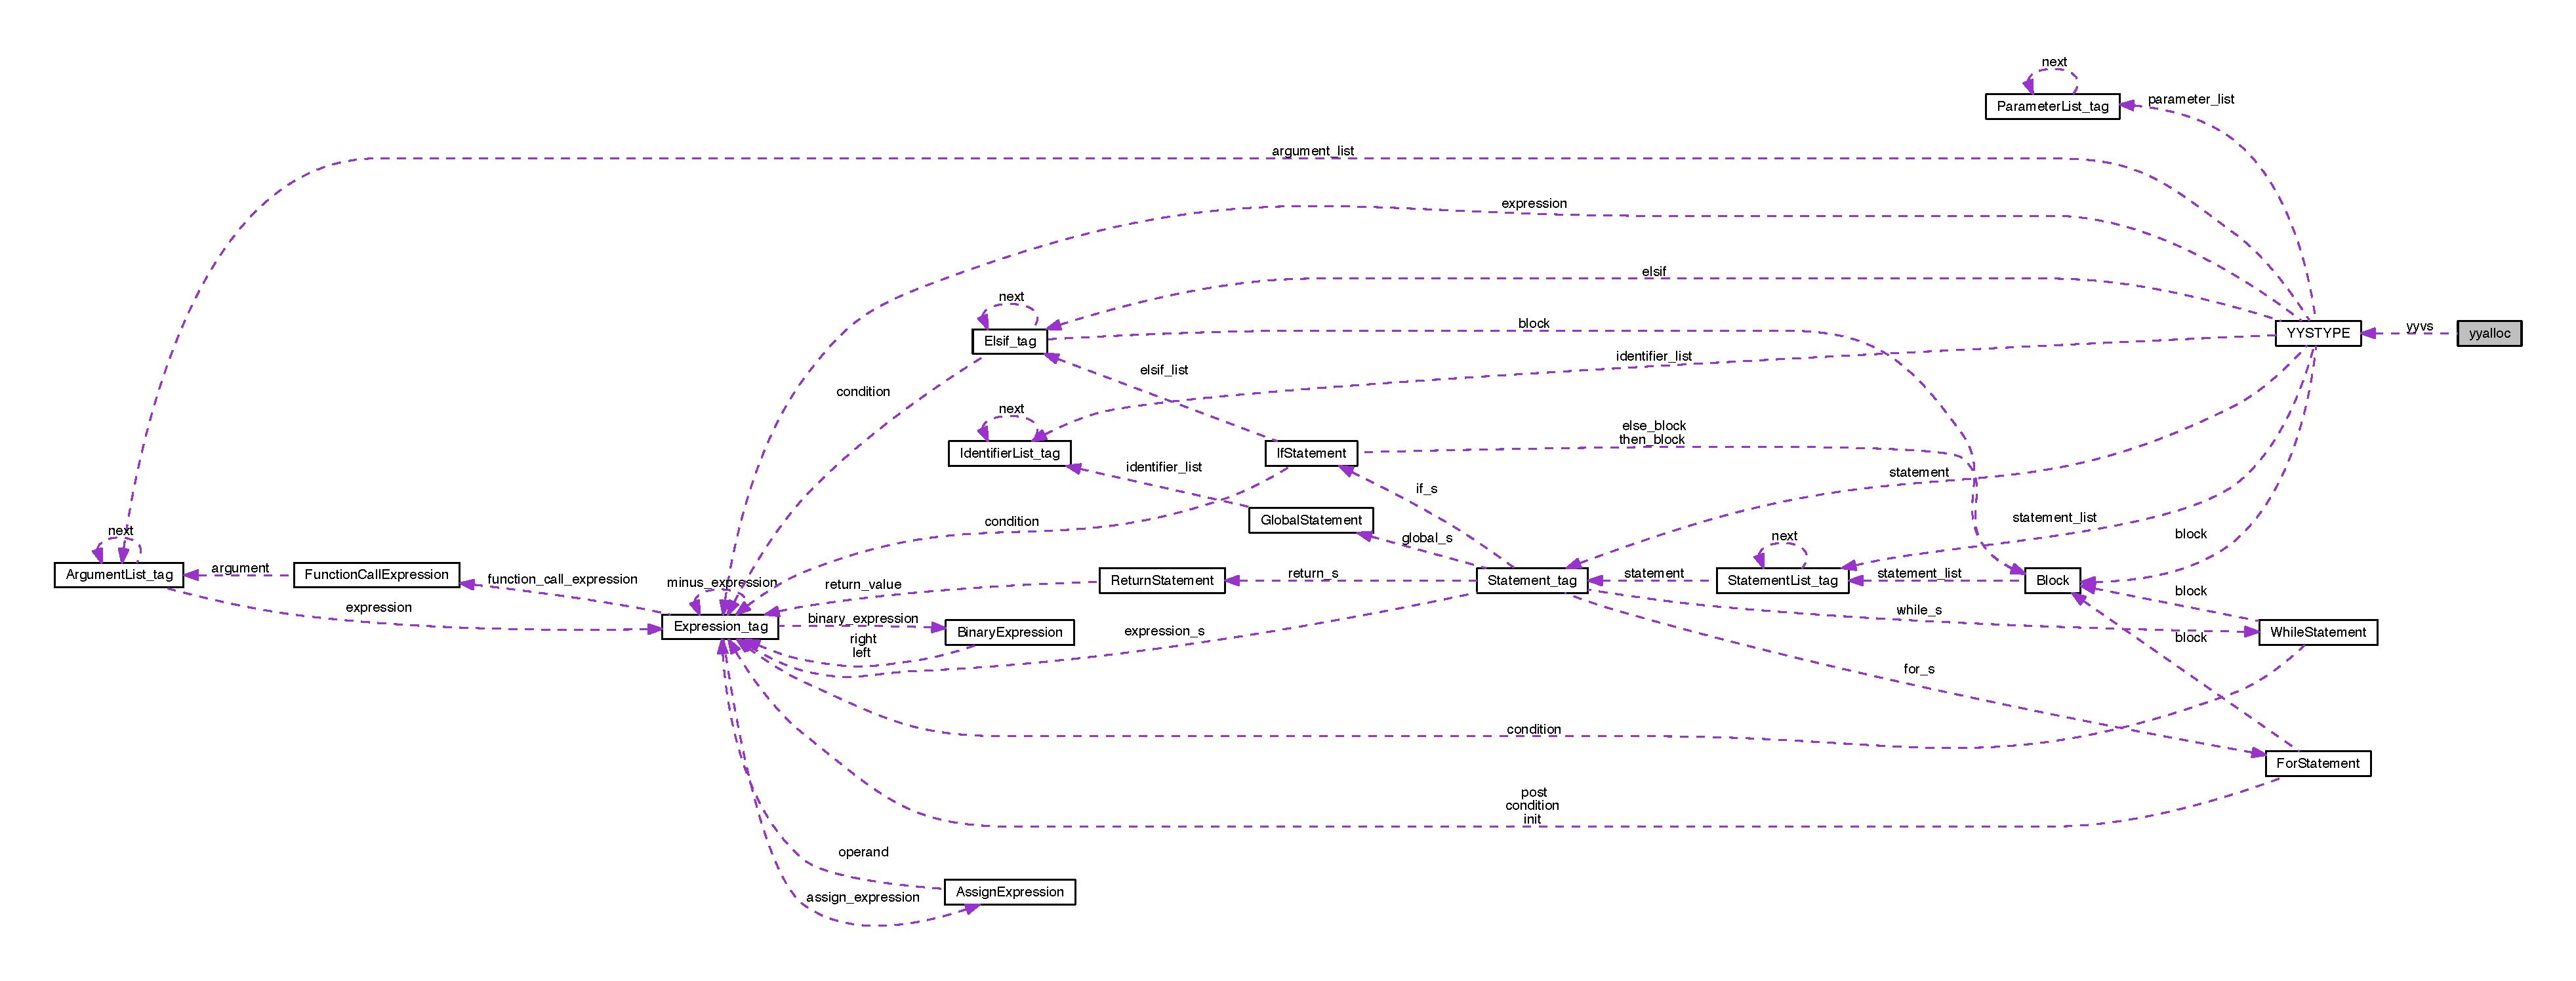
\includegraphics[width=350pt]{unionyyalloc__coll__graph}
\end{center}
\end{figure}
\subsection*{Public Attributes}
\begin{DoxyCompactItemize}
\item 
\hyperlink{y_8tab_8c_ade5b97f0021a4f6c5922ead3744ab297}{yytype\+\_\+int16} \hyperlink{unionyyalloc_aad44e4a724037e32eeb58333c516bb45}{yyss}
\item 
\hyperlink{union_y_y_s_t_y_p_e}{Y\+Y\+S\+T\+Y\+P\+E} \hyperlink{unionyyalloc_a9494cc8d8cd0eba1b44ca20fe89de5d2}{yyvs}
\end{DoxyCompactItemize}


\subsection{Member Data Documentation}
\hypertarget{unionyyalloc_aad44e4a724037e32eeb58333c516bb45}{}\index{yyalloc@{yyalloc}!yyss@{yyss}}
\index{yyss@{yyss}!yyalloc@{yyalloc}}
\subsubsection[{yyss}]{\setlength{\rightskip}{0pt plus 5cm}{\bf yytype\+\_\+int16} yyalloc\+::yyss}\label{unionyyalloc_aad44e4a724037e32eeb58333c516bb45}
\hypertarget{unionyyalloc_a9494cc8d8cd0eba1b44ca20fe89de5d2}{}\index{yyalloc@{yyalloc}!yyvs@{yyvs}}
\index{yyvs@{yyvs}!yyalloc@{yyalloc}}
\subsubsection[{yyvs}]{\setlength{\rightskip}{0pt plus 5cm}{\bf Y\+Y\+S\+T\+Y\+P\+E} yyalloc\+::yyvs}\label{unionyyalloc_a9494cc8d8cd0eba1b44ca20fe89de5d2}


The documentation for this union was generated from the following file\+:\begin{DoxyCompactItemize}
\item 
\hyperlink{y_8tab_8c}{y.\+tab.\+c}\end{DoxyCompactItemize}

\hypertarget{union_y_y_s_t_y_p_e}{}\section{Y\+Y\+S\+T\+Y\+P\+E Union Reference}
\label{union_y_y_s_t_y_p_e}\index{Y\+Y\+S\+T\+Y\+P\+E@{Y\+Y\+S\+T\+Y\+P\+E}}


{\ttfamily \#include $<$y.\+tab.\+h$>$}



Collaboration diagram for Y\+Y\+S\+T\+Y\+P\+E\+:\nopagebreak
\begin{figure}[H]
\begin{center}
\leavevmode
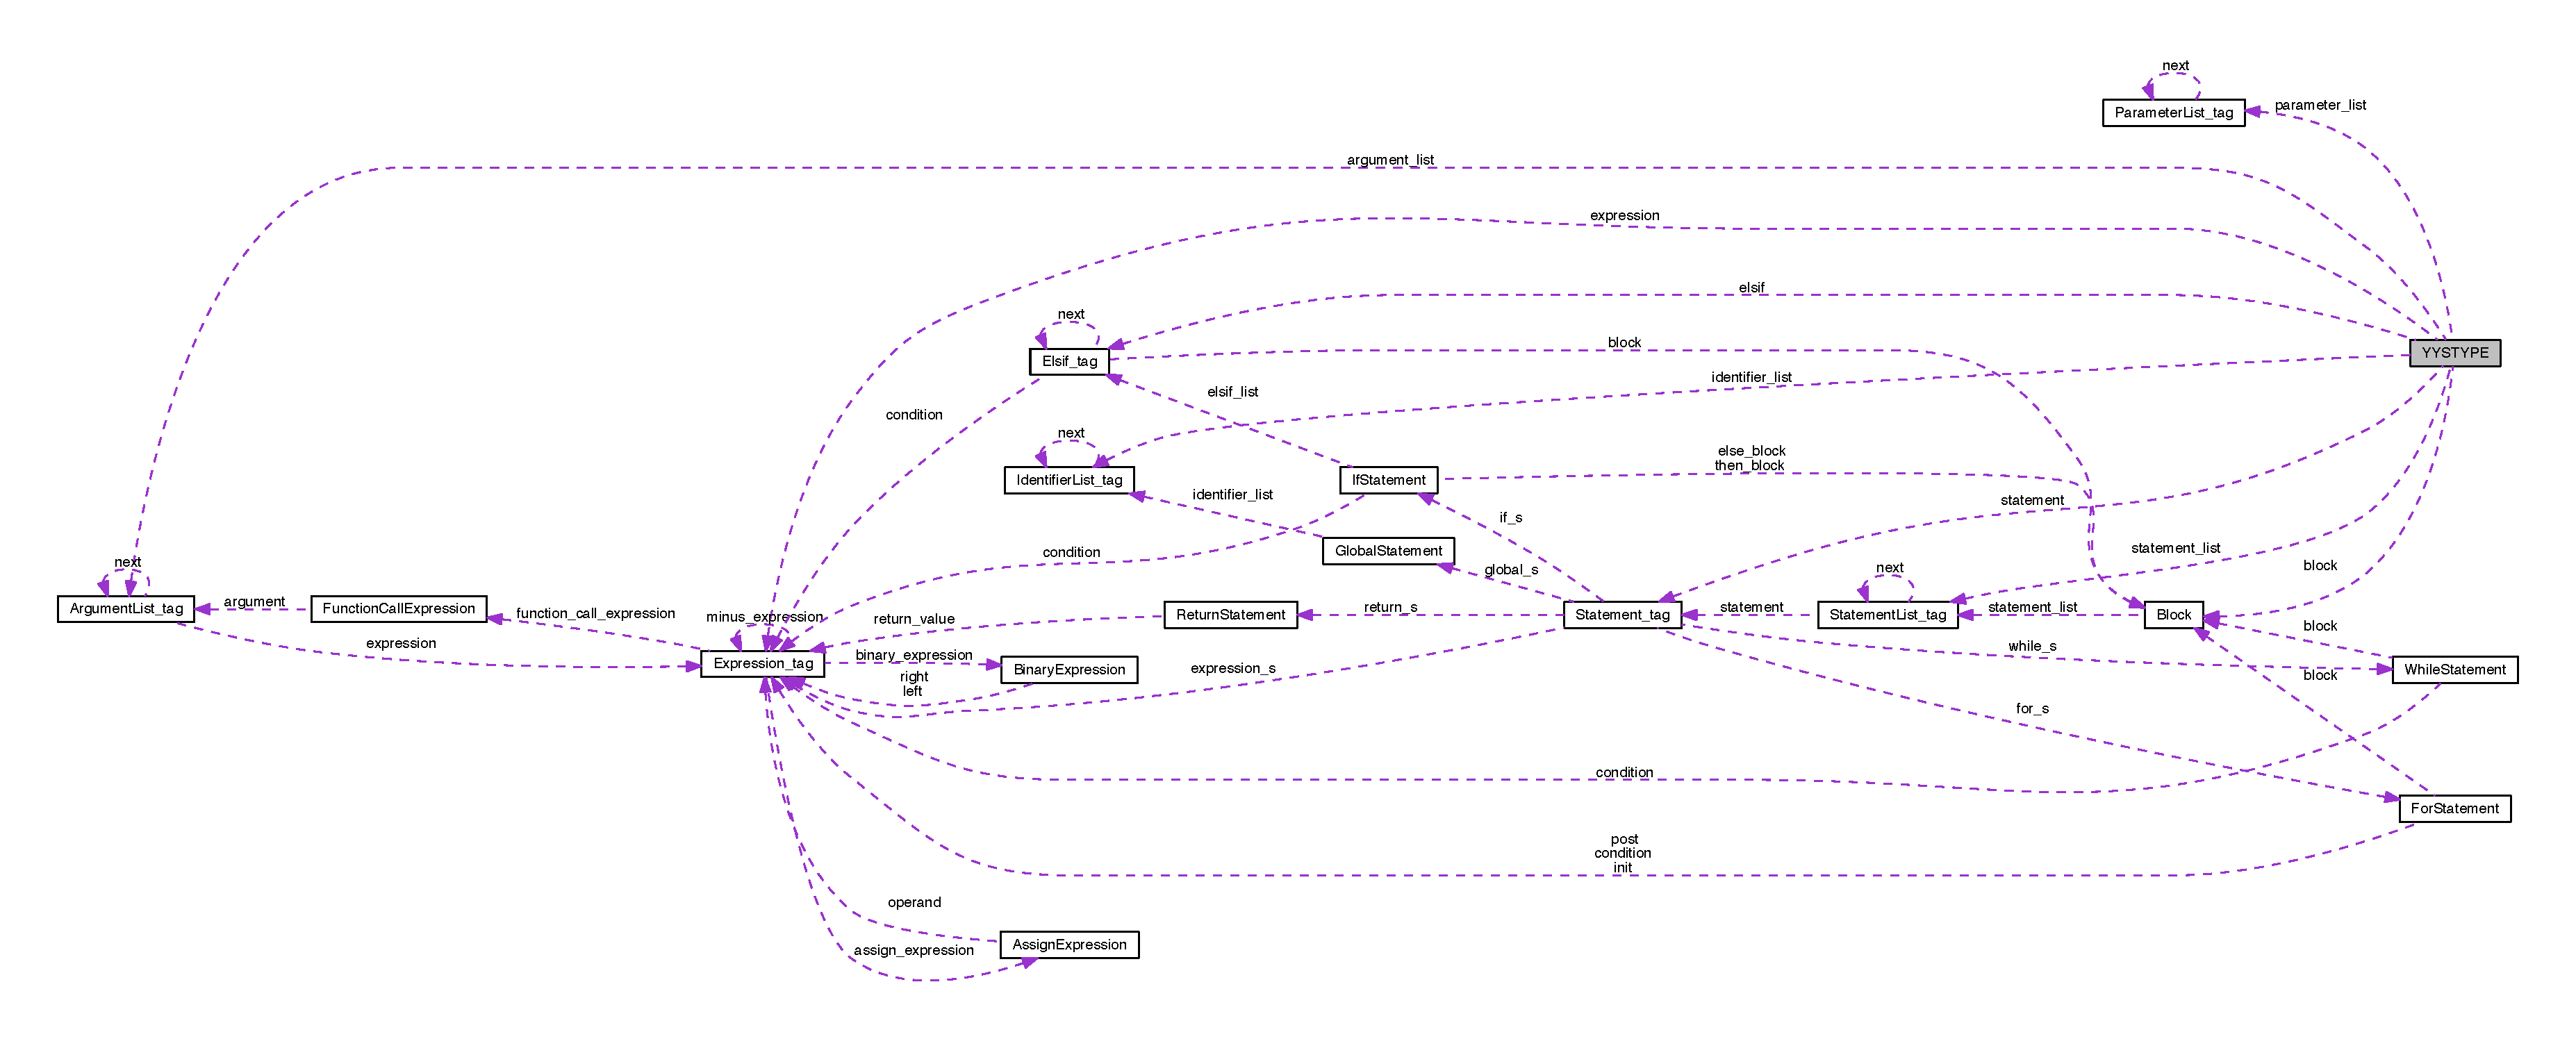
\includegraphics[width=350pt]{union_y_y_s_t_y_p_e__coll__graph}
\end{center}
\end{figure}
\subsection*{Public Attributes}
\begin{DoxyCompactItemize}
\item 
char $\ast$ \hyperlink{union_y_y_s_t_y_p_e_a90664571e9d5d6cabe4c478b7282b49a}{identifier}
\item 
\hyperlink{crowbar_8h_a7e7687e26b28e339ebcc8eaab571dcf7}{Parameter\+List} $\ast$ \hyperlink{union_y_y_s_t_y_p_e_afd386339b68e2828f86d0c0df7f20d5c}{parameter\+\_\+list}
\item 
\hyperlink{crowbar_8h_ad4ba12ca8ae3ead90081fb0aba63aff3}{Argument\+List} $\ast$ \hyperlink{union_y_y_s_t_y_p_e_a51ceba86a35a20a87f6e0989caf5e277}{argument\+\_\+list}
\item 
\hyperlink{crowbar_8h_a070c6feb370aad8a9665ca315bf6ed4a}{Expression} $\ast$ \hyperlink{union_y_y_s_t_y_p_e_a8be246867e8d03ea7dbd52816e021488}{expression}
\item 
\hyperlink{crowbar_8h_a16fe74a7a87df7652e815d139b3349d2}{Statement} $\ast$ \hyperlink{union_y_y_s_t_y_p_e_a3a91e31e5e63f3d04553e8c84a03a439}{statement}
\item 
\hyperlink{crowbar_8h_a8bffae51ec8146f480c3c14c61b4ff93}{Statement\+List} $\ast$ \hyperlink{union_y_y_s_t_y_p_e_a9ee5746ab7ab41340e386cf1b205c6a5}{statement\+\_\+list}
\item 
\hyperlink{struct_block}{Block} $\ast$ \hyperlink{union_y_y_s_t_y_p_e_a00c5fa03d994f87aa828a8000f2235e9}{block}
\item 
\hyperlink{crowbar_8h_a8d2ba32155a8a8a5a87e93c564061f1d}{Elsif} $\ast$ \hyperlink{union_y_y_s_t_y_p_e_a2b3478770181e47780aa7429d34c347a}{elsif}
\item 
\hyperlink{crowbar_8h_a3e8fd423ff4b73a7c5d557375f0a8741}{Identifier\+List} $\ast$ \hyperlink{union_y_y_s_t_y_p_e_a414528d10ba6151f9db97e991bf08ff0}{identifier\+\_\+list}
\end{DoxyCompactItemize}


\subsection{Member Data Documentation}
\hypertarget{union_y_y_s_t_y_p_e_a51ceba86a35a20a87f6e0989caf5e277}{}\index{Y\+Y\+S\+T\+Y\+P\+E@{Y\+Y\+S\+T\+Y\+P\+E}!argument\+\_\+list@{argument\+\_\+list}}
\index{argument\+\_\+list@{argument\+\_\+list}!Y\+Y\+S\+T\+Y\+P\+E@{Y\+Y\+S\+T\+Y\+P\+E}}
\subsubsection[{argument\+\_\+list}]{\setlength{\rightskip}{0pt plus 5cm}{\bf Argument\+List} $\ast$ Y\+Y\+S\+T\+Y\+P\+E\+::argument\+\_\+list}\label{union_y_y_s_t_y_p_e_a51ceba86a35a20a87f6e0989caf5e277}
\hypertarget{union_y_y_s_t_y_p_e_a00c5fa03d994f87aa828a8000f2235e9}{}\index{Y\+Y\+S\+T\+Y\+P\+E@{Y\+Y\+S\+T\+Y\+P\+E}!block@{block}}
\index{block@{block}!Y\+Y\+S\+T\+Y\+P\+E@{Y\+Y\+S\+T\+Y\+P\+E}}
\subsubsection[{block}]{\setlength{\rightskip}{0pt plus 5cm}{\bf Block} $\ast$ Y\+Y\+S\+T\+Y\+P\+E\+::block}\label{union_y_y_s_t_y_p_e_a00c5fa03d994f87aa828a8000f2235e9}
\hypertarget{union_y_y_s_t_y_p_e_a2b3478770181e47780aa7429d34c347a}{}\index{Y\+Y\+S\+T\+Y\+P\+E@{Y\+Y\+S\+T\+Y\+P\+E}!elsif@{elsif}}
\index{elsif@{elsif}!Y\+Y\+S\+T\+Y\+P\+E@{Y\+Y\+S\+T\+Y\+P\+E}}
\subsubsection[{elsif}]{\setlength{\rightskip}{0pt plus 5cm}{\bf Elsif} $\ast$ Y\+Y\+S\+T\+Y\+P\+E\+::elsif}\label{union_y_y_s_t_y_p_e_a2b3478770181e47780aa7429d34c347a}
\hypertarget{union_y_y_s_t_y_p_e_a8be246867e8d03ea7dbd52816e021488}{}\index{Y\+Y\+S\+T\+Y\+P\+E@{Y\+Y\+S\+T\+Y\+P\+E}!expression@{expression}}
\index{expression@{expression}!Y\+Y\+S\+T\+Y\+P\+E@{Y\+Y\+S\+T\+Y\+P\+E}}
\subsubsection[{expression}]{\setlength{\rightskip}{0pt plus 5cm}{\bf Expression} $\ast$ Y\+Y\+S\+T\+Y\+P\+E\+::expression}\label{union_y_y_s_t_y_p_e_a8be246867e8d03ea7dbd52816e021488}
\hypertarget{union_y_y_s_t_y_p_e_a90664571e9d5d6cabe4c478b7282b49a}{}\index{Y\+Y\+S\+T\+Y\+P\+E@{Y\+Y\+S\+T\+Y\+P\+E}!identifier@{identifier}}
\index{identifier@{identifier}!Y\+Y\+S\+T\+Y\+P\+E@{Y\+Y\+S\+T\+Y\+P\+E}}
\subsubsection[{identifier}]{\setlength{\rightskip}{0pt plus 5cm}char $\ast$ Y\+Y\+S\+T\+Y\+P\+E\+::identifier}\label{union_y_y_s_t_y_p_e_a90664571e9d5d6cabe4c478b7282b49a}
\hypertarget{union_y_y_s_t_y_p_e_a414528d10ba6151f9db97e991bf08ff0}{}\index{Y\+Y\+S\+T\+Y\+P\+E@{Y\+Y\+S\+T\+Y\+P\+E}!identifier\+\_\+list@{identifier\+\_\+list}}
\index{identifier\+\_\+list@{identifier\+\_\+list}!Y\+Y\+S\+T\+Y\+P\+E@{Y\+Y\+S\+T\+Y\+P\+E}}
\subsubsection[{identifier\+\_\+list}]{\setlength{\rightskip}{0pt plus 5cm}{\bf Identifier\+List} $\ast$ Y\+Y\+S\+T\+Y\+P\+E\+::identifier\+\_\+list}\label{union_y_y_s_t_y_p_e_a414528d10ba6151f9db97e991bf08ff0}
\hypertarget{union_y_y_s_t_y_p_e_afd386339b68e2828f86d0c0df7f20d5c}{}\index{Y\+Y\+S\+T\+Y\+P\+E@{Y\+Y\+S\+T\+Y\+P\+E}!parameter\+\_\+list@{parameter\+\_\+list}}
\index{parameter\+\_\+list@{parameter\+\_\+list}!Y\+Y\+S\+T\+Y\+P\+E@{Y\+Y\+S\+T\+Y\+P\+E}}
\subsubsection[{parameter\+\_\+list}]{\setlength{\rightskip}{0pt plus 5cm}{\bf Parameter\+List} $\ast$ Y\+Y\+S\+T\+Y\+P\+E\+::parameter\+\_\+list}\label{union_y_y_s_t_y_p_e_afd386339b68e2828f86d0c0df7f20d5c}
\hypertarget{union_y_y_s_t_y_p_e_a3a91e31e5e63f3d04553e8c84a03a439}{}\index{Y\+Y\+S\+T\+Y\+P\+E@{Y\+Y\+S\+T\+Y\+P\+E}!statement@{statement}}
\index{statement@{statement}!Y\+Y\+S\+T\+Y\+P\+E@{Y\+Y\+S\+T\+Y\+P\+E}}
\subsubsection[{statement}]{\setlength{\rightskip}{0pt plus 5cm}{\bf Statement} $\ast$ Y\+Y\+S\+T\+Y\+P\+E\+::statement}\label{union_y_y_s_t_y_p_e_a3a91e31e5e63f3d04553e8c84a03a439}
\hypertarget{union_y_y_s_t_y_p_e_a9ee5746ab7ab41340e386cf1b205c6a5}{}\index{Y\+Y\+S\+T\+Y\+P\+E@{Y\+Y\+S\+T\+Y\+P\+E}!statement\+\_\+list@{statement\+\_\+list}}
\index{statement\+\_\+list@{statement\+\_\+list}!Y\+Y\+S\+T\+Y\+P\+E@{Y\+Y\+S\+T\+Y\+P\+E}}
\subsubsection[{statement\+\_\+list}]{\setlength{\rightskip}{0pt plus 5cm}{\bf Statement\+List} $\ast$ Y\+Y\+S\+T\+Y\+P\+E\+::statement\+\_\+list}\label{union_y_y_s_t_y_p_e_a9ee5746ab7ab41340e386cf1b205c6a5}


The documentation for this union was generated from the following files\+:\begin{DoxyCompactItemize}
\item 
\hyperlink{y_8tab_8c}{y.\+tab.\+c}\item 
\hyperlink{y_8tab_8h}{y.\+tab.\+h}\end{DoxyCompactItemize}

\chapter{File Documentation}
\hypertarget{_c_r_b_8h}{}\section{C\+R\+B.\+h File Reference}
\label{_c_r_b_8h}\index{C\+R\+B.\+h@{C\+R\+B.\+h}}
{\ttfamily \#include $<$stdio.\+h$>$}\\*
Include dependency graph for C\+R\+B.\+h\+:\nopagebreak
\begin{figure}[H]
\begin{center}
\leavevmode
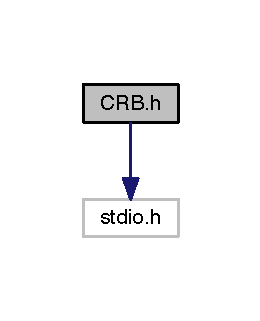
\includegraphics[width=125pt]{_c_r_b_8h__incl}
\end{center}
\end{figure}
This graph shows which files directly or indirectly include this file\+:\nopagebreak
\begin{figure}[H]
\begin{center}
\leavevmode
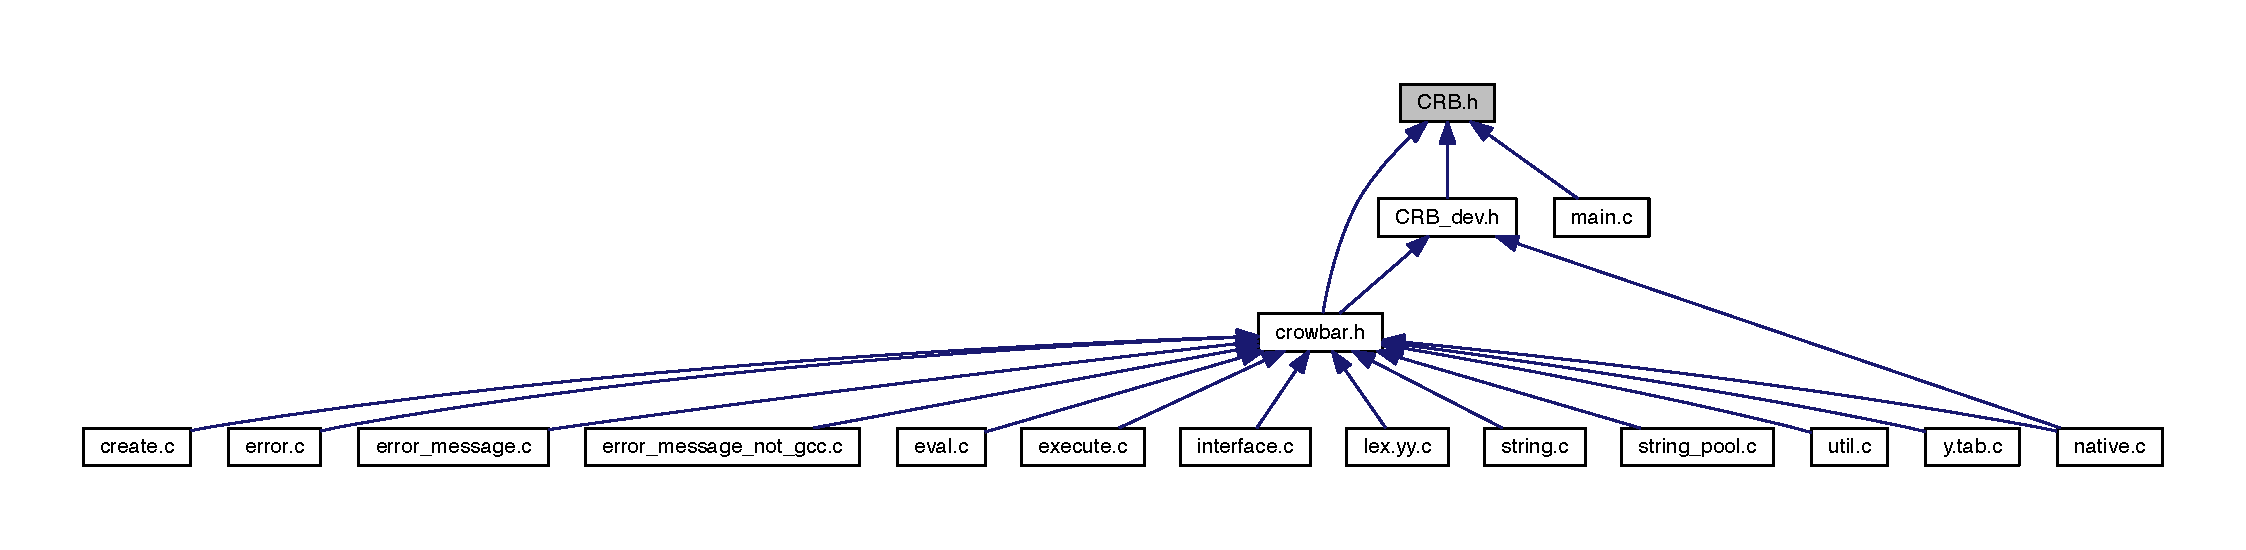
\includegraphics[width=350pt]{_c_r_b_8h__dep__incl}
\end{center}
\end{figure}
\subsection*{Typedefs}
\begin{DoxyCompactItemize}
\item 
typedef struct \hyperlink{struct_c_r_b___interpreter__tag}{C\+R\+B\+\_\+\+Interpreter\+\_\+tag} \hyperlink{_c_r_b_8h_a5b6eeccc92c5aa79d6051a9f80ecb710}{C\+R\+B\+\_\+\+Interpreter}
\end{DoxyCompactItemize}
\subsection*{Functions}
\begin{DoxyCompactItemize}
\item 
\hyperlink{_c_r_b_8h_a5b6eeccc92c5aa79d6051a9f80ecb710}{C\+R\+B\+\_\+\+Interpreter} $\ast$ \hyperlink{_c_r_b_8h_ad3220c824ee390ae66a6fd09f25b1b40}{C\+R\+B\+\_\+create\+\_\+interpreter} (void)
\item 
void \hyperlink{_c_r_b_8h_a141508c6454f35d4362e762b4006d9ee}{C\+R\+B\+\_\+compile} (\hyperlink{_c_r_b_8h_a5b6eeccc92c5aa79d6051a9f80ecb710}{C\+R\+B\+\_\+\+Interpreter} $\ast$interpreter, F\+I\+L\+E $\ast$fp)
\item 
void \hyperlink{_c_r_b_8h_a09ed7f3ac7d3b3bb6bd00e2f1a69d2b2}{C\+R\+B\+\_\+interpret} (\hyperlink{_c_r_b_8h_a5b6eeccc92c5aa79d6051a9f80ecb710}{C\+R\+B\+\_\+\+Interpreter} $\ast$interpreter)
\item 
void \hyperlink{_c_r_b_8h_a0bbde3973064ac8ff4aa073fd5183b3a}{C\+R\+B\+\_\+dispose\+\_\+interpreter} (\hyperlink{_c_r_b_8h_a5b6eeccc92c5aa79d6051a9f80ecb710}{C\+R\+B\+\_\+\+Interpreter} $\ast$interpreter)
\end{DoxyCompactItemize}


\subsection{Typedef Documentation}
\hypertarget{_c_r_b_8h_a5b6eeccc92c5aa79d6051a9f80ecb710}{}\index{C\+R\+B.\+h@{C\+R\+B.\+h}!C\+R\+B\+\_\+\+Interpreter@{C\+R\+B\+\_\+\+Interpreter}}
\index{C\+R\+B\+\_\+\+Interpreter@{C\+R\+B\+\_\+\+Interpreter}!C\+R\+B.\+h@{C\+R\+B.\+h}}
\subsubsection[{C\+R\+B\+\_\+\+Interpreter}]{\setlength{\rightskip}{0pt plus 5cm}typedef struct {\bf C\+R\+B\+\_\+\+Interpreter\+\_\+tag} {\bf C\+R\+B\+\_\+\+Interpreter}}\label{_c_r_b_8h_a5b6eeccc92c5aa79d6051a9f80ecb710}


\subsection{Function Documentation}
\hypertarget{_c_r_b_8h_a141508c6454f35d4362e762b4006d9ee}{}\index{C\+R\+B.\+h@{C\+R\+B.\+h}!C\+R\+B\+\_\+compile@{C\+R\+B\+\_\+compile}}
\index{C\+R\+B\+\_\+compile@{C\+R\+B\+\_\+compile}!C\+R\+B.\+h@{C\+R\+B.\+h}}
\subsubsection[{C\+R\+B\+\_\+compile(\+C\+R\+B\+\_\+\+Interpreter $\ast$interpreter, F\+I\+L\+E $\ast$fp)}]{\setlength{\rightskip}{0pt plus 5cm}void C\+R\+B\+\_\+compile (
\begin{DoxyParamCaption}
\item[{{\bf C\+R\+B\+\_\+\+Interpreter} $\ast$}]{interpreter, }
\item[{F\+I\+L\+E $\ast$}]{fp}
\end{DoxyParamCaption}
)}\label{_c_r_b_8h_a141508c6454f35d4362e762b4006d9ee}


Here is the call graph for this function\+:
\nopagebreak
\begin{figure}[H]
\begin{center}
\leavevmode
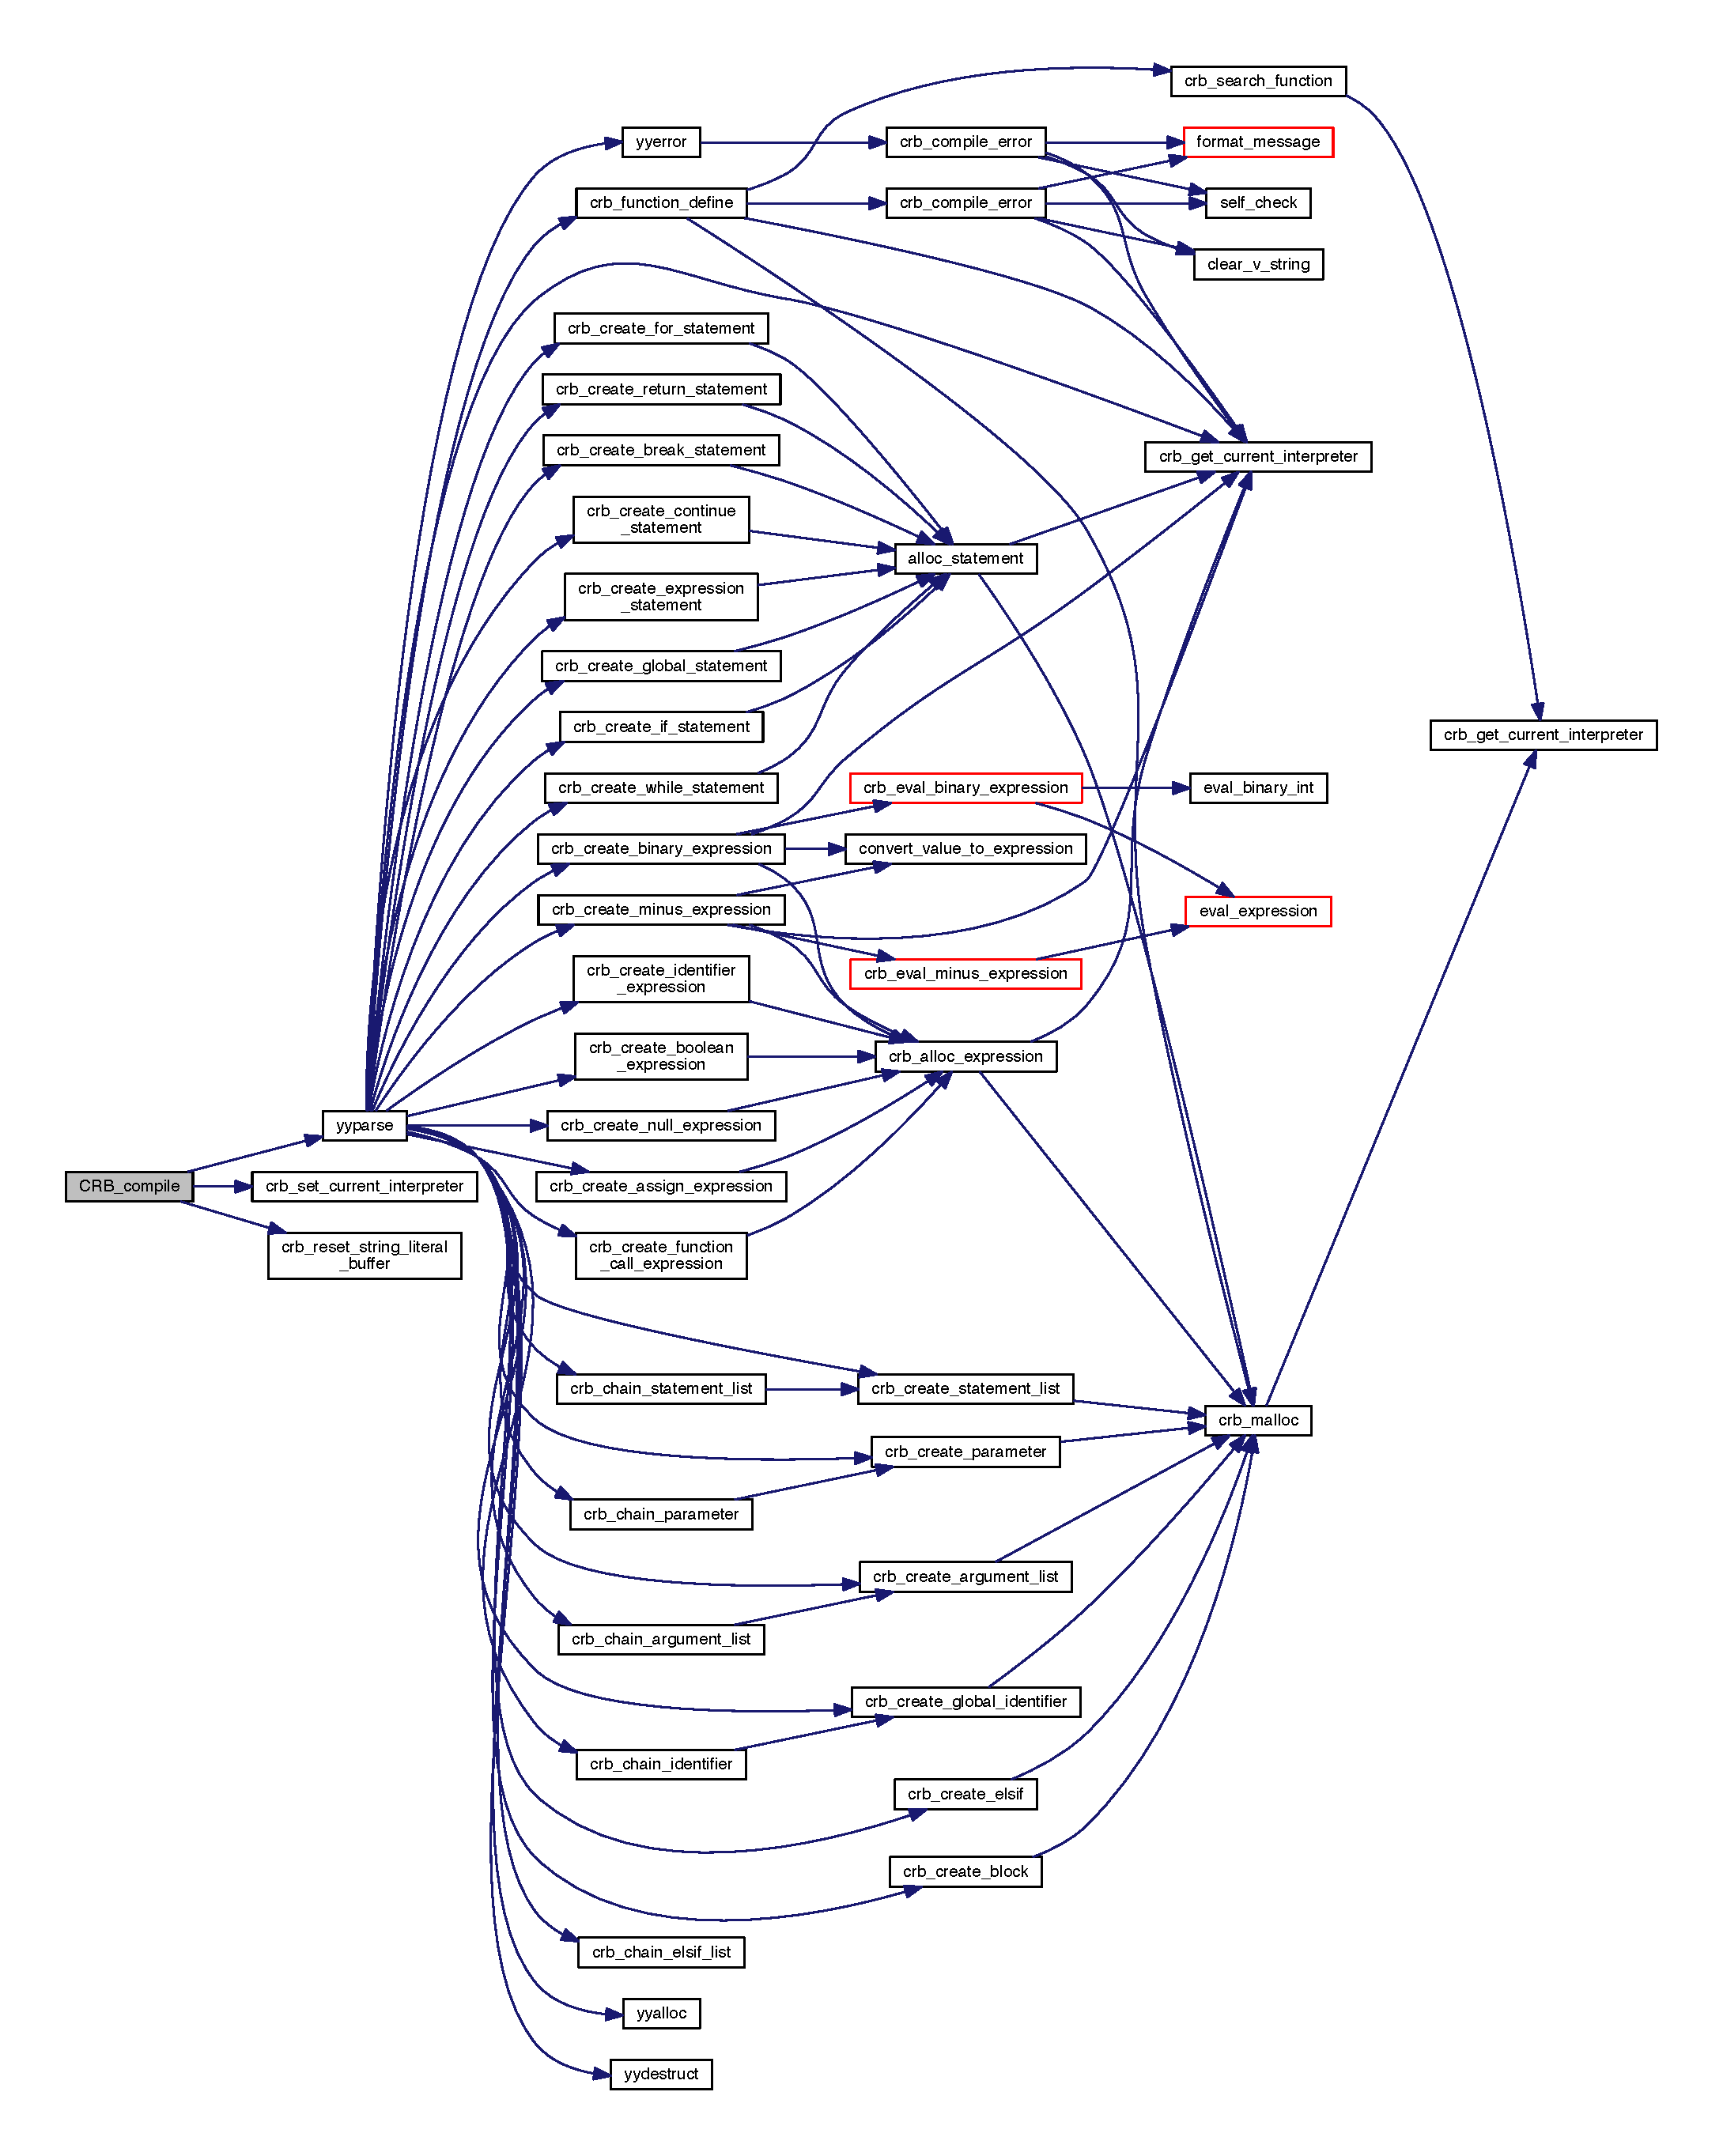
\includegraphics[width=350pt]{_c_r_b_8h_a141508c6454f35d4362e762b4006d9ee_cgraph}
\end{center}
\end{figure}




Here is the caller graph for this function\+:\nopagebreak
\begin{figure}[H]
\begin{center}
\leavevmode
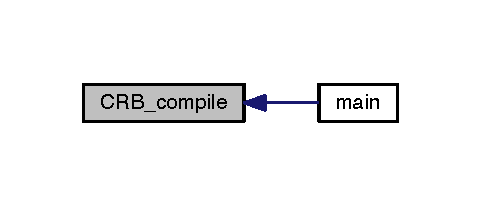
\includegraphics[width=231pt]{_c_r_b_8h_a141508c6454f35d4362e762b4006d9ee_icgraph}
\end{center}
\end{figure}


\hypertarget{_c_r_b_8h_ad3220c824ee390ae66a6fd09f25b1b40}{}\index{C\+R\+B.\+h@{C\+R\+B.\+h}!C\+R\+B\+\_\+create\+\_\+interpreter@{C\+R\+B\+\_\+create\+\_\+interpreter}}
\index{C\+R\+B\+\_\+create\+\_\+interpreter@{C\+R\+B\+\_\+create\+\_\+interpreter}!C\+R\+B.\+h@{C\+R\+B.\+h}}
\subsubsection[{C\+R\+B\+\_\+create\+\_\+interpreter(void)}]{\setlength{\rightskip}{0pt plus 5cm}{\bf C\+R\+B\+\_\+\+Interpreter}$\ast$ C\+R\+B\+\_\+create\+\_\+interpreter (
\begin{DoxyParamCaption}
\item[{void}]{}
\end{DoxyParamCaption}
)}\label{_c_r_b_8h_ad3220c824ee390ae66a6fd09f25b1b40}


Here is the call graph for this function\+:
\nopagebreak
\begin{figure}[H]
\begin{center}
\leavevmode
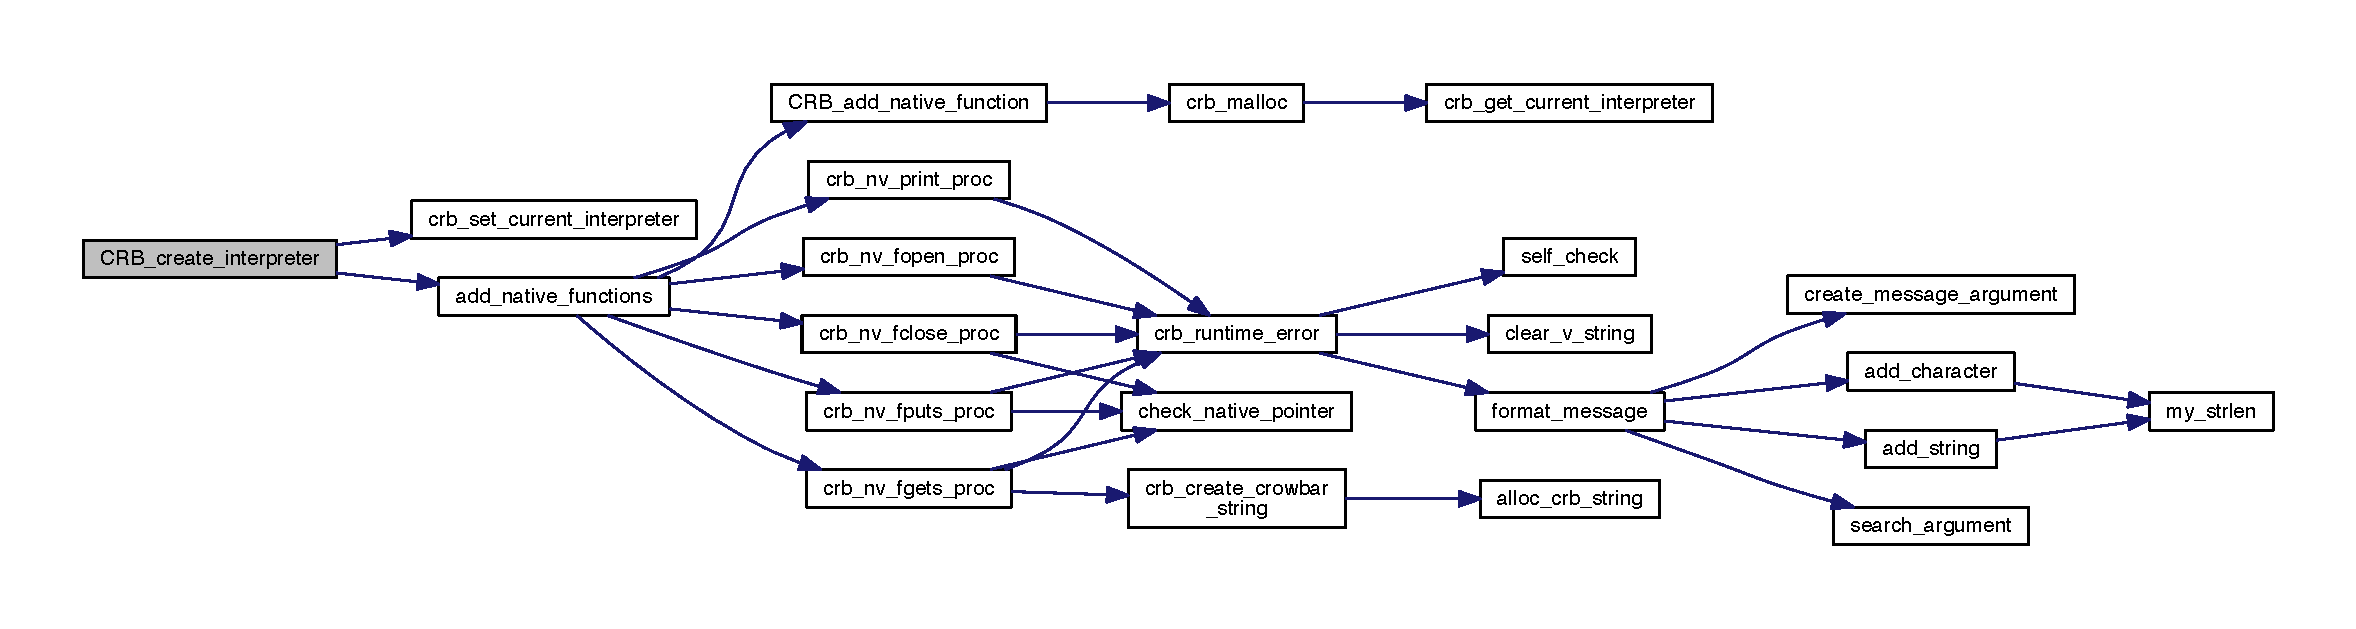
\includegraphics[width=350pt]{_c_r_b_8h_ad3220c824ee390ae66a6fd09f25b1b40_cgraph}
\end{center}
\end{figure}




Here is the caller graph for this function\+:\nopagebreak
\begin{figure}[H]
\begin{center}
\leavevmode
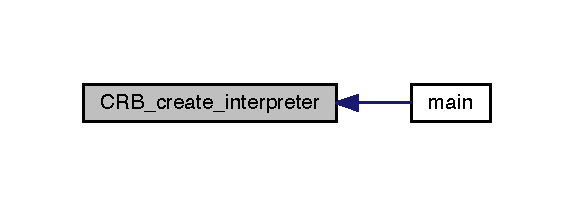
\includegraphics[width=275pt]{_c_r_b_8h_ad3220c824ee390ae66a6fd09f25b1b40_icgraph}
\end{center}
\end{figure}


\hypertarget{_c_r_b_8h_a0bbde3973064ac8ff4aa073fd5183b3a}{}\index{C\+R\+B.\+h@{C\+R\+B.\+h}!C\+R\+B\+\_\+dispose\+\_\+interpreter@{C\+R\+B\+\_\+dispose\+\_\+interpreter}}
\index{C\+R\+B\+\_\+dispose\+\_\+interpreter@{C\+R\+B\+\_\+dispose\+\_\+interpreter}!C\+R\+B.\+h@{C\+R\+B.\+h}}
\subsubsection[{C\+R\+B\+\_\+dispose\+\_\+interpreter(\+C\+R\+B\+\_\+\+Interpreter $\ast$interpreter)}]{\setlength{\rightskip}{0pt plus 5cm}void C\+R\+B\+\_\+dispose\+\_\+interpreter (
\begin{DoxyParamCaption}
\item[{{\bf C\+R\+B\+\_\+\+Interpreter} $\ast$}]{interpreter}
\end{DoxyParamCaption}
)}\label{_c_r_b_8h_a0bbde3973064ac8ff4aa073fd5183b3a}


Here is the call graph for this function\+:
\nopagebreak
\begin{figure}[H]
\begin{center}
\leavevmode
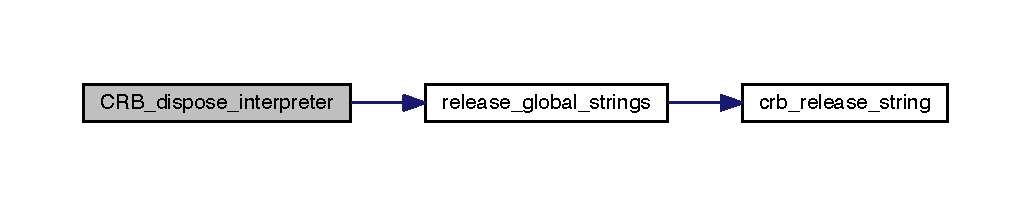
\includegraphics[width=350pt]{_c_r_b_8h_a0bbde3973064ac8ff4aa073fd5183b3a_cgraph}
\end{center}
\end{figure}




Here is the caller graph for this function\+:\nopagebreak
\begin{figure}[H]
\begin{center}
\leavevmode
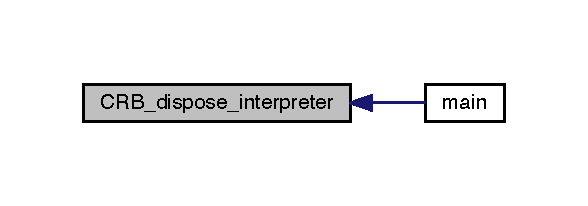
\includegraphics[width=282pt]{_c_r_b_8h_a0bbde3973064ac8ff4aa073fd5183b3a_icgraph}
\end{center}
\end{figure}


\hypertarget{_c_r_b_8h_a09ed7f3ac7d3b3bb6bd00e2f1a69d2b2}{}\index{C\+R\+B.\+h@{C\+R\+B.\+h}!C\+R\+B\+\_\+interpret@{C\+R\+B\+\_\+interpret}}
\index{C\+R\+B\+\_\+interpret@{C\+R\+B\+\_\+interpret}!C\+R\+B.\+h@{C\+R\+B.\+h}}
\subsubsection[{C\+R\+B\+\_\+interpret(\+C\+R\+B\+\_\+\+Interpreter $\ast$interpreter)}]{\setlength{\rightskip}{0pt plus 5cm}void C\+R\+B\+\_\+interpret (
\begin{DoxyParamCaption}
\item[{{\bf C\+R\+B\+\_\+\+Interpreter} $\ast$}]{interpreter}
\end{DoxyParamCaption}
)}\label{_c_r_b_8h_a09ed7f3ac7d3b3bb6bd00e2f1a69d2b2}


Here is the call graph for this function\+:
\nopagebreak
\begin{figure}[H]
\begin{center}
\leavevmode
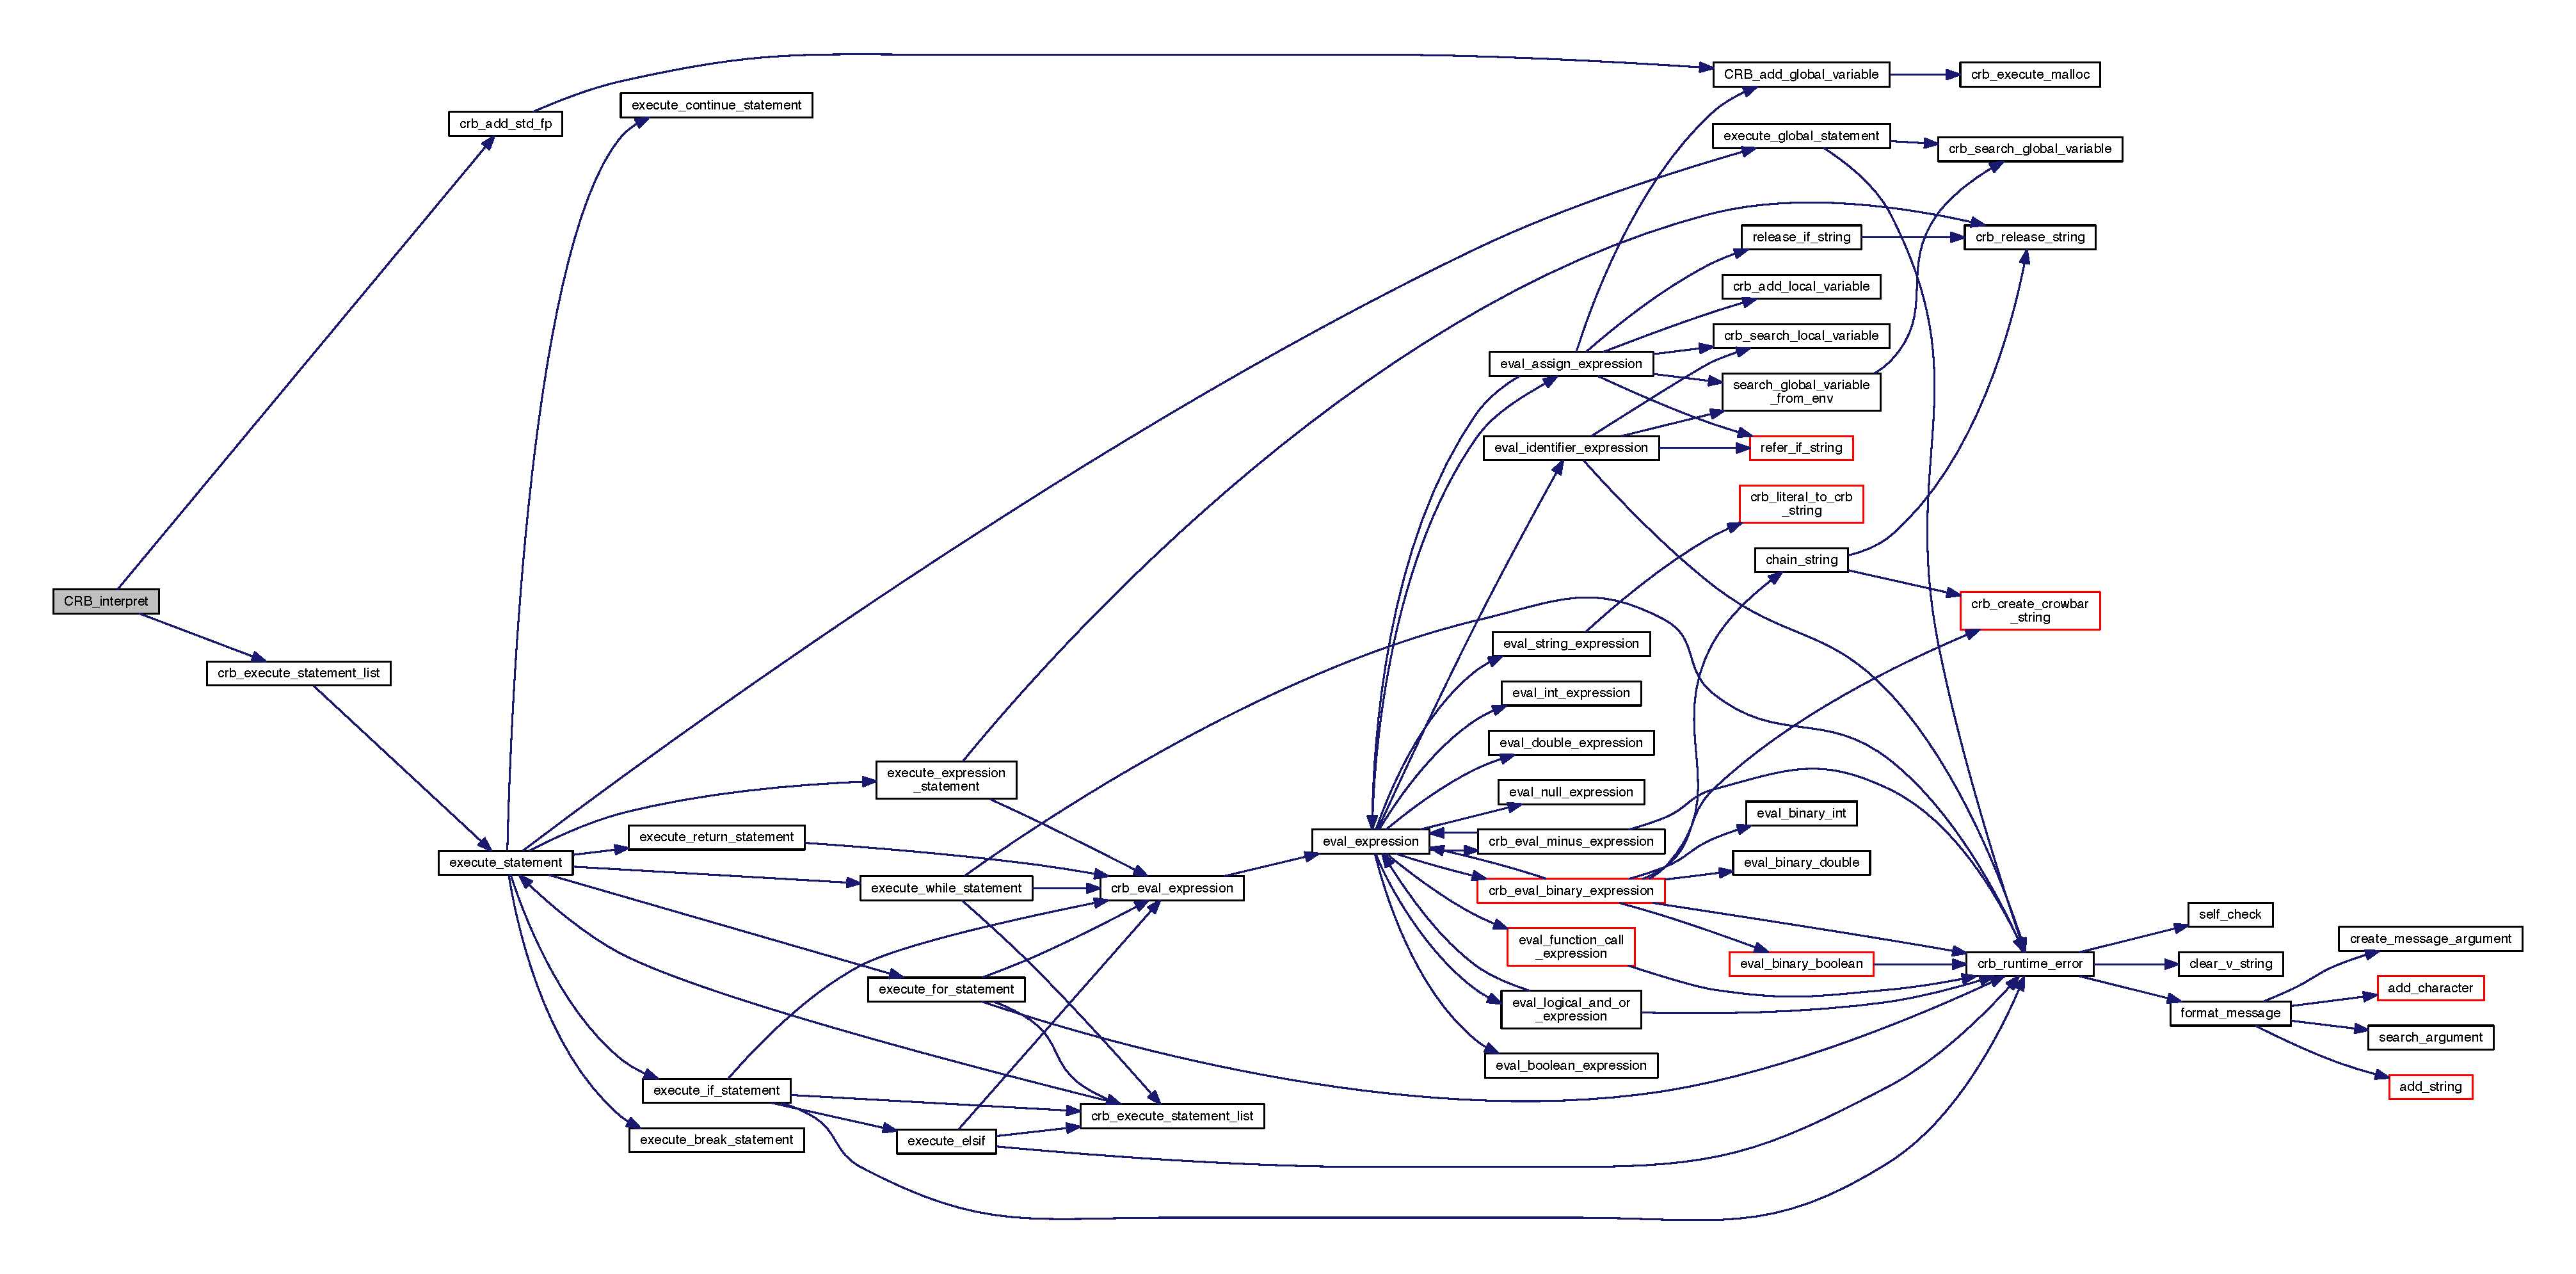
\includegraphics[width=350pt]{_c_r_b_8h_a09ed7f3ac7d3b3bb6bd00e2f1a69d2b2_cgraph}
\end{center}
\end{figure}




Here is the caller graph for this function\+:\nopagebreak
\begin{figure}[H]
\begin{center}
\leavevmode
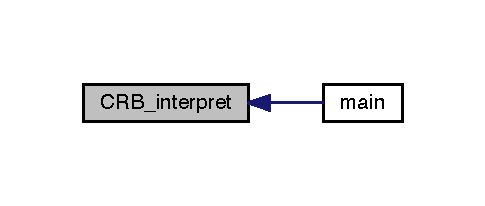
\includegraphics[width=233pt]{_c_r_b_8h_a09ed7f3ac7d3b3bb6bd00e2f1a69d2b2_icgraph}
\end{center}
\end{figure}



\hypertarget{_c_r_b__dev_8h}{}\section{C\+R\+B\+\_\+dev.\+h File Reference}
\label{_c_r_b__dev_8h}\index{C\+R\+B\+\_\+dev.\+h@{C\+R\+B\+\_\+dev.\+h}}
{\ttfamily \#include \char`\"{}C\+R\+B.\+h\char`\"{}}\\*
Include dependency graph for C\+R\+B\+\_\+dev.\+h\+:\nopagebreak
\begin{figure}[H]
\begin{center}
\leavevmode
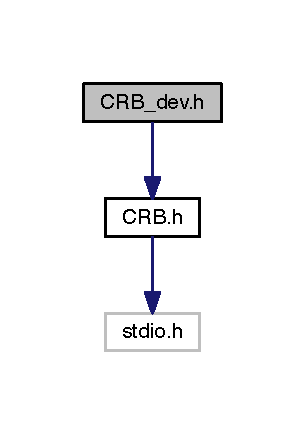
\includegraphics[width=146pt]{_c_r_b__dev_8h__incl}
\end{center}
\end{figure}
This graph shows which files directly or indirectly include this file\+:\nopagebreak
\begin{figure}[H]
\begin{center}
\leavevmode
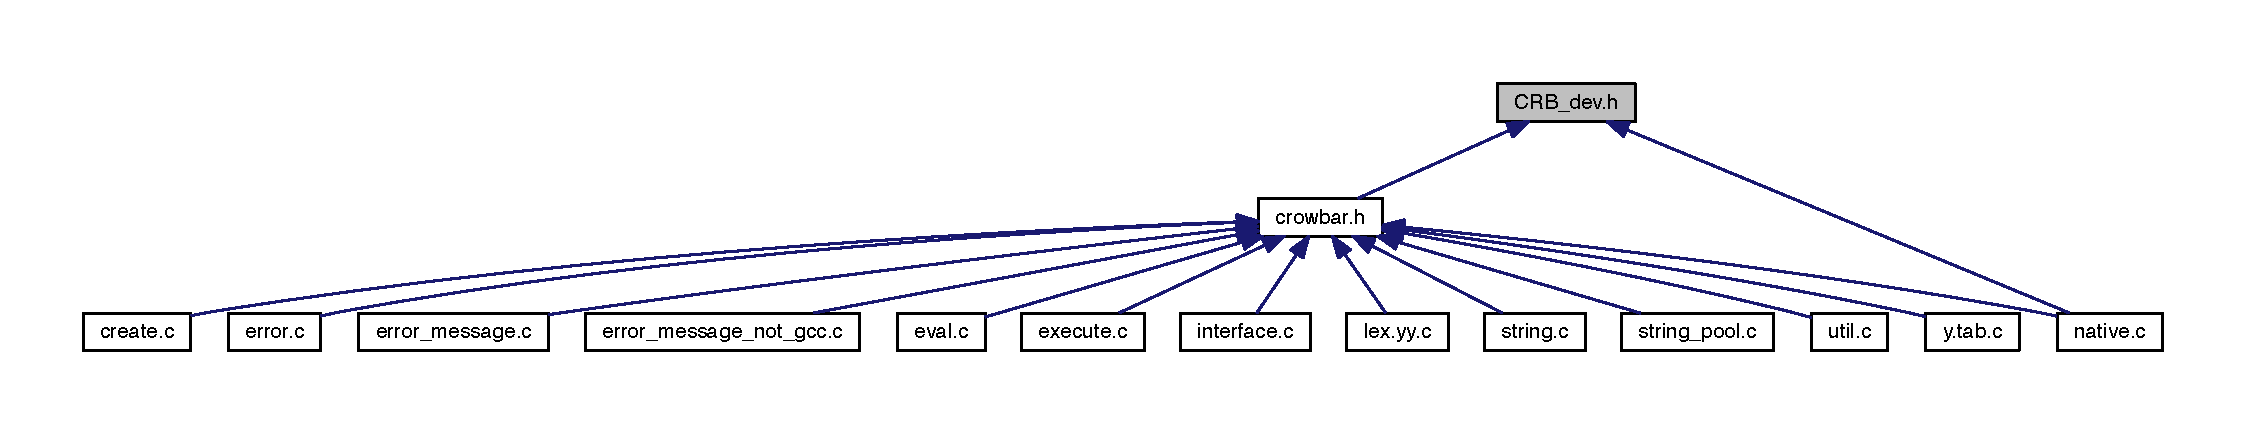
\includegraphics[width=350pt]{_c_r_b__dev_8h__dep__incl}
\end{center}
\end{figure}
\subsection*{Classes}
\begin{DoxyCompactItemize}
\item 
struct \hyperlink{struct_c_r_b___native_pointer_info}{C\+R\+B\+\_\+\+Native\+Pointer\+Info}
\item 
struct \hyperlink{struct_c_r_b___native_pointer}{C\+R\+B\+\_\+\+Native\+Pointer}
\item 
struct \hyperlink{struct_c_r_b___value}{C\+R\+B\+\_\+\+Value}
\end{DoxyCompactItemize}
\subsection*{Typedefs}
\begin{DoxyCompactItemize}
\item 
typedef struct \hyperlink{struct_c_r_b___string__tag}{C\+R\+B\+\_\+\+String\+\_\+tag} \hyperlink{_c_r_b__dev_8h_a0372b51b327f3425e983d9924fc713f8}{C\+R\+B\+\_\+\+String}
\item 
typedef \hyperlink{struct_c_r_b___value}{C\+R\+B\+\_\+\+Value} \hyperlink{_c_r_b__dev_8h_af310ef1ce709cc9c2e7d1e3bf43b76ec}{C\+R\+B\+\_\+\+Native\+Function\+Proc}(\hyperlink{_c_r_b_8h_a5b6eeccc92c5aa79d6051a9f80ecb710}{C\+R\+B\+\_\+\+Interpreter} $\ast$interpreter, int arg\+\_\+count, \hyperlink{struct_c_r_b___value}{C\+R\+B\+\_\+\+Value} $\ast$args)
\end{DoxyCompactItemize}
\subsection*{Enumerations}
\begin{DoxyCompactItemize}
\item 
enum \hyperlink{_c_r_b__dev_8h_a5000f2b447c9132c07d7f1cf66134a69}{C\+R\+B\+\_\+\+Boolean} \{ \hyperlink{_c_r_b__dev_8h_a5000f2b447c9132c07d7f1cf66134a69a3d4eb7009bc7437d1c978e086432b2e4}{C\+R\+B\+\_\+\+F\+A\+L\+S\+E} = 0, 
\hyperlink{_c_r_b__dev_8h_a5000f2b447c9132c07d7f1cf66134a69a20ab77152ed9064df421b9e1817fe54a}{C\+R\+B\+\_\+\+T\+R\+U\+E} = 1
 \}
\item 
enum \hyperlink{_c_r_b__dev_8h_a1a82f38e78e95951e6a9cdc0f5fd4a3a}{C\+R\+B\+\_\+\+Value\+Type} \{ \\*
\hyperlink{_c_r_b__dev_8h_a1a82f38e78e95951e6a9cdc0f5fd4a3aa2d7452b3b4b07ada7dc9bf705dfb74dd}{C\+R\+B\+\_\+\+B\+O\+O\+L\+E\+A\+N\+\_\+\+V\+A\+L\+U\+E} = 1, 
\hyperlink{_c_r_b__dev_8h_a1a82f38e78e95951e6a9cdc0f5fd4a3aac389348731301821f648c333f92a5a5b}{C\+R\+B\+\_\+\+I\+N\+T\+\_\+\+V\+A\+L\+U\+E}, 
\hyperlink{_c_r_b__dev_8h_a1a82f38e78e95951e6a9cdc0f5fd4a3aaa592697b11ce804be060838de0cf9200}{C\+R\+B\+\_\+\+D\+O\+U\+B\+L\+E\+\_\+\+V\+A\+L\+U\+E}, 
\hyperlink{_c_r_b__dev_8h_a1a82f38e78e95951e6a9cdc0f5fd4a3aacf8dc7d28dacce6299639023795c5e83}{C\+R\+B\+\_\+\+S\+T\+R\+I\+N\+G\+\_\+\+V\+A\+L\+U\+E}, 
\\*
\hyperlink{_c_r_b__dev_8h_a1a82f38e78e95951e6a9cdc0f5fd4a3aa0b5b84b6cf3b558153aa23e75c8a5b01}{C\+R\+B\+\_\+\+N\+A\+T\+I\+V\+E\+\_\+\+P\+O\+I\+N\+T\+E\+R\+\_\+\+V\+A\+L\+U\+E}, 
\hyperlink{_c_r_b__dev_8h_a1a82f38e78e95951e6a9cdc0f5fd4a3aabc822550d26192008084e3b49d0d7dec}{C\+R\+B\+\_\+\+N\+U\+L\+L\+\_\+\+V\+A\+L\+U\+E}
 \}
\end{DoxyCompactItemize}
\subsection*{Functions}
\begin{DoxyCompactItemize}
\item 
void \hyperlink{_c_r_b__dev_8h_a940149828fe093b31374c316022a981a}{C\+R\+B\+\_\+add\+\_\+native\+\_\+function} (\hyperlink{_c_r_b_8h_a5b6eeccc92c5aa79d6051a9f80ecb710}{C\+R\+B\+\_\+\+Interpreter} $\ast$interpreter, char $\ast$name, \hyperlink{_c_r_b__dev_8h_af310ef1ce709cc9c2e7d1e3bf43b76ec}{C\+R\+B\+\_\+\+Native\+Function\+Proc} $\ast$proc)
\item 
void \hyperlink{_c_r_b__dev_8h_aa4e2d1a292b2c1d9cacba9e06ecdc022}{C\+R\+B\+\_\+add\+\_\+global\+\_\+variable} (\hyperlink{_c_r_b_8h_a5b6eeccc92c5aa79d6051a9f80ecb710}{C\+R\+B\+\_\+\+Interpreter} $\ast$inter, char $\ast$identifier, \hyperlink{struct_c_r_b___value}{C\+R\+B\+\_\+\+Value} $\ast$value)
\end{DoxyCompactItemize}


\subsection{Typedef Documentation}
\hypertarget{_c_r_b__dev_8h_af310ef1ce709cc9c2e7d1e3bf43b76ec}{}\index{C\+R\+B\+\_\+dev.\+h@{C\+R\+B\+\_\+dev.\+h}!C\+R\+B\+\_\+\+Native\+Function\+Proc@{C\+R\+B\+\_\+\+Native\+Function\+Proc}}
\index{C\+R\+B\+\_\+\+Native\+Function\+Proc@{C\+R\+B\+\_\+\+Native\+Function\+Proc}!C\+R\+B\+\_\+dev.\+h@{C\+R\+B\+\_\+dev.\+h}}
\subsubsection[{C\+R\+B\+\_\+\+Native\+Function\+Proc}]{\setlength{\rightskip}{0pt plus 5cm}typedef {\bf C\+R\+B\+\_\+\+Value} C\+R\+B\+\_\+\+Native\+Function\+Proc({\bf C\+R\+B\+\_\+\+Interpreter} $\ast$interpreter, int arg\+\_\+count, {\bf C\+R\+B\+\_\+\+Value} $\ast$args)}\label{_c_r_b__dev_8h_af310ef1ce709cc9c2e7d1e3bf43b76ec}
\hypertarget{_c_r_b__dev_8h_a0372b51b327f3425e983d9924fc713f8}{}\index{C\+R\+B\+\_\+dev.\+h@{C\+R\+B\+\_\+dev.\+h}!C\+R\+B\+\_\+\+String@{C\+R\+B\+\_\+\+String}}
\index{C\+R\+B\+\_\+\+String@{C\+R\+B\+\_\+\+String}!C\+R\+B\+\_\+dev.\+h@{C\+R\+B\+\_\+dev.\+h}}
\subsubsection[{C\+R\+B\+\_\+\+String}]{\setlength{\rightskip}{0pt plus 5cm}typedef struct {\bf C\+R\+B\+\_\+\+String\+\_\+tag} {\bf C\+R\+B\+\_\+\+String}}\label{_c_r_b__dev_8h_a0372b51b327f3425e983d9924fc713f8}


\subsection{Enumeration Type Documentation}
\hypertarget{_c_r_b__dev_8h_a5000f2b447c9132c07d7f1cf66134a69}{}\index{C\+R\+B\+\_\+dev.\+h@{C\+R\+B\+\_\+dev.\+h}!C\+R\+B\+\_\+\+Boolean@{C\+R\+B\+\_\+\+Boolean}}
\index{C\+R\+B\+\_\+\+Boolean@{C\+R\+B\+\_\+\+Boolean}!C\+R\+B\+\_\+dev.\+h@{C\+R\+B\+\_\+dev.\+h}}
\subsubsection[{C\+R\+B\+\_\+\+Boolean}]{\setlength{\rightskip}{0pt plus 5cm}enum {\bf C\+R\+B\+\_\+\+Boolean}}\label{_c_r_b__dev_8h_a5000f2b447c9132c07d7f1cf66134a69}
\begin{Desc}
\item[Enumerator]\par
\begin{description}
\index{C\+R\+B\+\_\+\+F\+A\+L\+S\+E@{C\+R\+B\+\_\+\+F\+A\+L\+S\+E}!C\+R\+B\+\_\+dev.\+h@{C\+R\+B\+\_\+dev.\+h}}\index{C\+R\+B\+\_\+dev.\+h@{C\+R\+B\+\_\+dev.\+h}!C\+R\+B\+\_\+\+F\+A\+L\+S\+E@{C\+R\+B\+\_\+\+F\+A\+L\+S\+E}}\item[{\em 
\hypertarget{_c_r_b__dev_8h_a5000f2b447c9132c07d7f1cf66134a69a3d4eb7009bc7437d1c978e086432b2e4}{}C\+R\+B\+\_\+\+F\+A\+L\+S\+E\label{_c_r_b__dev_8h_a5000f2b447c9132c07d7f1cf66134a69a3d4eb7009bc7437d1c978e086432b2e4}
}]\index{C\+R\+B\+\_\+\+T\+R\+U\+E@{C\+R\+B\+\_\+\+T\+R\+U\+E}!C\+R\+B\+\_\+dev.\+h@{C\+R\+B\+\_\+dev.\+h}}\index{C\+R\+B\+\_\+dev.\+h@{C\+R\+B\+\_\+dev.\+h}!C\+R\+B\+\_\+\+T\+R\+U\+E@{C\+R\+B\+\_\+\+T\+R\+U\+E}}\item[{\em 
\hypertarget{_c_r_b__dev_8h_a5000f2b447c9132c07d7f1cf66134a69a20ab77152ed9064df421b9e1817fe54a}{}C\+R\+B\+\_\+\+T\+R\+U\+E\label{_c_r_b__dev_8h_a5000f2b447c9132c07d7f1cf66134a69a20ab77152ed9064df421b9e1817fe54a}
}]\end{description}
\end{Desc}
\hypertarget{_c_r_b__dev_8h_a1a82f38e78e95951e6a9cdc0f5fd4a3a}{}\index{C\+R\+B\+\_\+dev.\+h@{C\+R\+B\+\_\+dev.\+h}!C\+R\+B\+\_\+\+Value\+Type@{C\+R\+B\+\_\+\+Value\+Type}}
\index{C\+R\+B\+\_\+\+Value\+Type@{C\+R\+B\+\_\+\+Value\+Type}!C\+R\+B\+\_\+dev.\+h@{C\+R\+B\+\_\+dev.\+h}}
\subsubsection[{C\+R\+B\+\_\+\+Value\+Type}]{\setlength{\rightskip}{0pt plus 5cm}enum {\bf C\+R\+B\+\_\+\+Value\+Type}}\label{_c_r_b__dev_8h_a1a82f38e78e95951e6a9cdc0f5fd4a3a}
\begin{Desc}
\item[Enumerator]\par
\begin{description}
\index{C\+R\+B\+\_\+\+B\+O\+O\+L\+E\+A\+N\+\_\+\+V\+A\+L\+U\+E@{C\+R\+B\+\_\+\+B\+O\+O\+L\+E\+A\+N\+\_\+\+V\+A\+L\+U\+E}!C\+R\+B\+\_\+dev.\+h@{C\+R\+B\+\_\+dev.\+h}}\index{C\+R\+B\+\_\+dev.\+h@{C\+R\+B\+\_\+dev.\+h}!C\+R\+B\+\_\+\+B\+O\+O\+L\+E\+A\+N\+\_\+\+V\+A\+L\+U\+E@{C\+R\+B\+\_\+\+B\+O\+O\+L\+E\+A\+N\+\_\+\+V\+A\+L\+U\+E}}\item[{\em 
\hypertarget{_c_r_b__dev_8h_a1a82f38e78e95951e6a9cdc0f5fd4a3aa2d7452b3b4b07ada7dc9bf705dfb74dd}{}C\+R\+B\+\_\+\+B\+O\+O\+L\+E\+A\+N\+\_\+\+V\+A\+L\+U\+E\label{_c_r_b__dev_8h_a1a82f38e78e95951e6a9cdc0f5fd4a3aa2d7452b3b4b07ada7dc9bf705dfb74dd}
}]\index{C\+R\+B\+\_\+\+I\+N\+T\+\_\+\+V\+A\+L\+U\+E@{C\+R\+B\+\_\+\+I\+N\+T\+\_\+\+V\+A\+L\+U\+E}!C\+R\+B\+\_\+dev.\+h@{C\+R\+B\+\_\+dev.\+h}}\index{C\+R\+B\+\_\+dev.\+h@{C\+R\+B\+\_\+dev.\+h}!C\+R\+B\+\_\+\+I\+N\+T\+\_\+\+V\+A\+L\+U\+E@{C\+R\+B\+\_\+\+I\+N\+T\+\_\+\+V\+A\+L\+U\+E}}\item[{\em 
\hypertarget{_c_r_b__dev_8h_a1a82f38e78e95951e6a9cdc0f5fd4a3aac389348731301821f648c333f92a5a5b}{}C\+R\+B\+\_\+\+I\+N\+T\+\_\+\+V\+A\+L\+U\+E\label{_c_r_b__dev_8h_a1a82f38e78e95951e6a9cdc0f5fd4a3aac389348731301821f648c333f92a5a5b}
}]\index{C\+R\+B\+\_\+\+D\+O\+U\+B\+L\+E\+\_\+\+V\+A\+L\+U\+E@{C\+R\+B\+\_\+\+D\+O\+U\+B\+L\+E\+\_\+\+V\+A\+L\+U\+E}!C\+R\+B\+\_\+dev.\+h@{C\+R\+B\+\_\+dev.\+h}}\index{C\+R\+B\+\_\+dev.\+h@{C\+R\+B\+\_\+dev.\+h}!C\+R\+B\+\_\+\+D\+O\+U\+B\+L\+E\+\_\+\+V\+A\+L\+U\+E@{C\+R\+B\+\_\+\+D\+O\+U\+B\+L\+E\+\_\+\+V\+A\+L\+U\+E}}\item[{\em 
\hypertarget{_c_r_b__dev_8h_a1a82f38e78e95951e6a9cdc0f5fd4a3aaa592697b11ce804be060838de0cf9200}{}C\+R\+B\+\_\+\+D\+O\+U\+B\+L\+E\+\_\+\+V\+A\+L\+U\+E\label{_c_r_b__dev_8h_a1a82f38e78e95951e6a9cdc0f5fd4a3aaa592697b11ce804be060838de0cf9200}
}]\index{C\+R\+B\+\_\+\+S\+T\+R\+I\+N\+G\+\_\+\+V\+A\+L\+U\+E@{C\+R\+B\+\_\+\+S\+T\+R\+I\+N\+G\+\_\+\+V\+A\+L\+U\+E}!C\+R\+B\+\_\+dev.\+h@{C\+R\+B\+\_\+dev.\+h}}\index{C\+R\+B\+\_\+dev.\+h@{C\+R\+B\+\_\+dev.\+h}!C\+R\+B\+\_\+\+S\+T\+R\+I\+N\+G\+\_\+\+V\+A\+L\+U\+E@{C\+R\+B\+\_\+\+S\+T\+R\+I\+N\+G\+\_\+\+V\+A\+L\+U\+E}}\item[{\em 
\hypertarget{_c_r_b__dev_8h_a1a82f38e78e95951e6a9cdc0f5fd4a3aacf8dc7d28dacce6299639023795c5e83}{}C\+R\+B\+\_\+\+S\+T\+R\+I\+N\+G\+\_\+\+V\+A\+L\+U\+E\label{_c_r_b__dev_8h_a1a82f38e78e95951e6a9cdc0f5fd4a3aacf8dc7d28dacce6299639023795c5e83}
}]\index{C\+R\+B\+\_\+\+N\+A\+T\+I\+V\+E\+\_\+\+P\+O\+I\+N\+T\+E\+R\+\_\+\+V\+A\+L\+U\+E@{C\+R\+B\+\_\+\+N\+A\+T\+I\+V\+E\+\_\+\+P\+O\+I\+N\+T\+E\+R\+\_\+\+V\+A\+L\+U\+E}!C\+R\+B\+\_\+dev.\+h@{C\+R\+B\+\_\+dev.\+h}}\index{C\+R\+B\+\_\+dev.\+h@{C\+R\+B\+\_\+dev.\+h}!C\+R\+B\+\_\+\+N\+A\+T\+I\+V\+E\+\_\+\+P\+O\+I\+N\+T\+E\+R\+\_\+\+V\+A\+L\+U\+E@{C\+R\+B\+\_\+\+N\+A\+T\+I\+V\+E\+\_\+\+P\+O\+I\+N\+T\+E\+R\+\_\+\+V\+A\+L\+U\+E}}\item[{\em 
\hypertarget{_c_r_b__dev_8h_a1a82f38e78e95951e6a9cdc0f5fd4a3aa0b5b84b6cf3b558153aa23e75c8a5b01}{}C\+R\+B\+\_\+\+N\+A\+T\+I\+V\+E\+\_\+\+P\+O\+I\+N\+T\+E\+R\+\_\+\+V\+A\+L\+U\+E\label{_c_r_b__dev_8h_a1a82f38e78e95951e6a9cdc0f5fd4a3aa0b5b84b6cf3b558153aa23e75c8a5b01}
}]\index{C\+R\+B\+\_\+\+N\+U\+L\+L\+\_\+\+V\+A\+L\+U\+E@{C\+R\+B\+\_\+\+N\+U\+L\+L\+\_\+\+V\+A\+L\+U\+E}!C\+R\+B\+\_\+dev.\+h@{C\+R\+B\+\_\+dev.\+h}}\index{C\+R\+B\+\_\+dev.\+h@{C\+R\+B\+\_\+dev.\+h}!C\+R\+B\+\_\+\+N\+U\+L\+L\+\_\+\+V\+A\+L\+U\+E@{C\+R\+B\+\_\+\+N\+U\+L\+L\+\_\+\+V\+A\+L\+U\+E}}\item[{\em 
\hypertarget{_c_r_b__dev_8h_a1a82f38e78e95951e6a9cdc0f5fd4a3aabc822550d26192008084e3b49d0d7dec}{}C\+R\+B\+\_\+\+N\+U\+L\+L\+\_\+\+V\+A\+L\+U\+E\label{_c_r_b__dev_8h_a1a82f38e78e95951e6a9cdc0f5fd4a3aabc822550d26192008084e3b49d0d7dec}
}]\end{description}
\end{Desc}


\subsection{Function Documentation}
\hypertarget{_c_r_b__dev_8h_aa4e2d1a292b2c1d9cacba9e06ecdc022}{}\index{C\+R\+B\+\_\+dev.\+h@{C\+R\+B\+\_\+dev.\+h}!C\+R\+B\+\_\+add\+\_\+global\+\_\+variable@{C\+R\+B\+\_\+add\+\_\+global\+\_\+variable}}
\index{C\+R\+B\+\_\+add\+\_\+global\+\_\+variable@{C\+R\+B\+\_\+add\+\_\+global\+\_\+variable}!C\+R\+B\+\_\+dev.\+h@{C\+R\+B\+\_\+dev.\+h}}
\subsubsection[{C\+R\+B\+\_\+add\+\_\+global\+\_\+variable(\+C\+R\+B\+\_\+\+Interpreter $\ast$inter, char $\ast$identifier, C\+R\+B\+\_\+\+Value $\ast$value)}]{\setlength{\rightskip}{0pt plus 5cm}void C\+R\+B\+\_\+add\+\_\+global\+\_\+variable (
\begin{DoxyParamCaption}
\item[{{\bf C\+R\+B\+\_\+\+Interpreter} $\ast$}]{inter, }
\item[{char $\ast$}]{identifier, }
\item[{{\bf C\+R\+B\+\_\+\+Value} $\ast$}]{value}
\end{DoxyParamCaption}
)}\label{_c_r_b__dev_8h_aa4e2d1a292b2c1d9cacba9e06ecdc022}


Here is the call graph for this function\+:\nopagebreak
\begin{figure}[H]
\begin{center}
\leavevmode
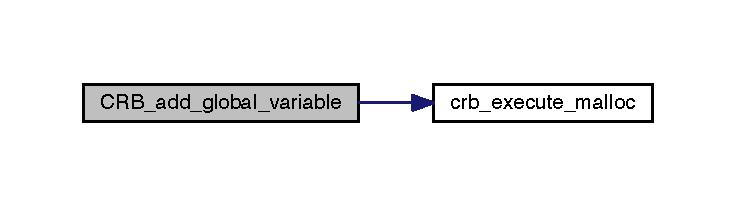
\includegraphics[width=350pt]{_c_r_b__dev_8h_aa4e2d1a292b2c1d9cacba9e06ecdc022_cgraph}
\end{center}
\end{figure}




Here is the caller graph for this function\+:
\nopagebreak
\begin{figure}[H]
\begin{center}
\leavevmode
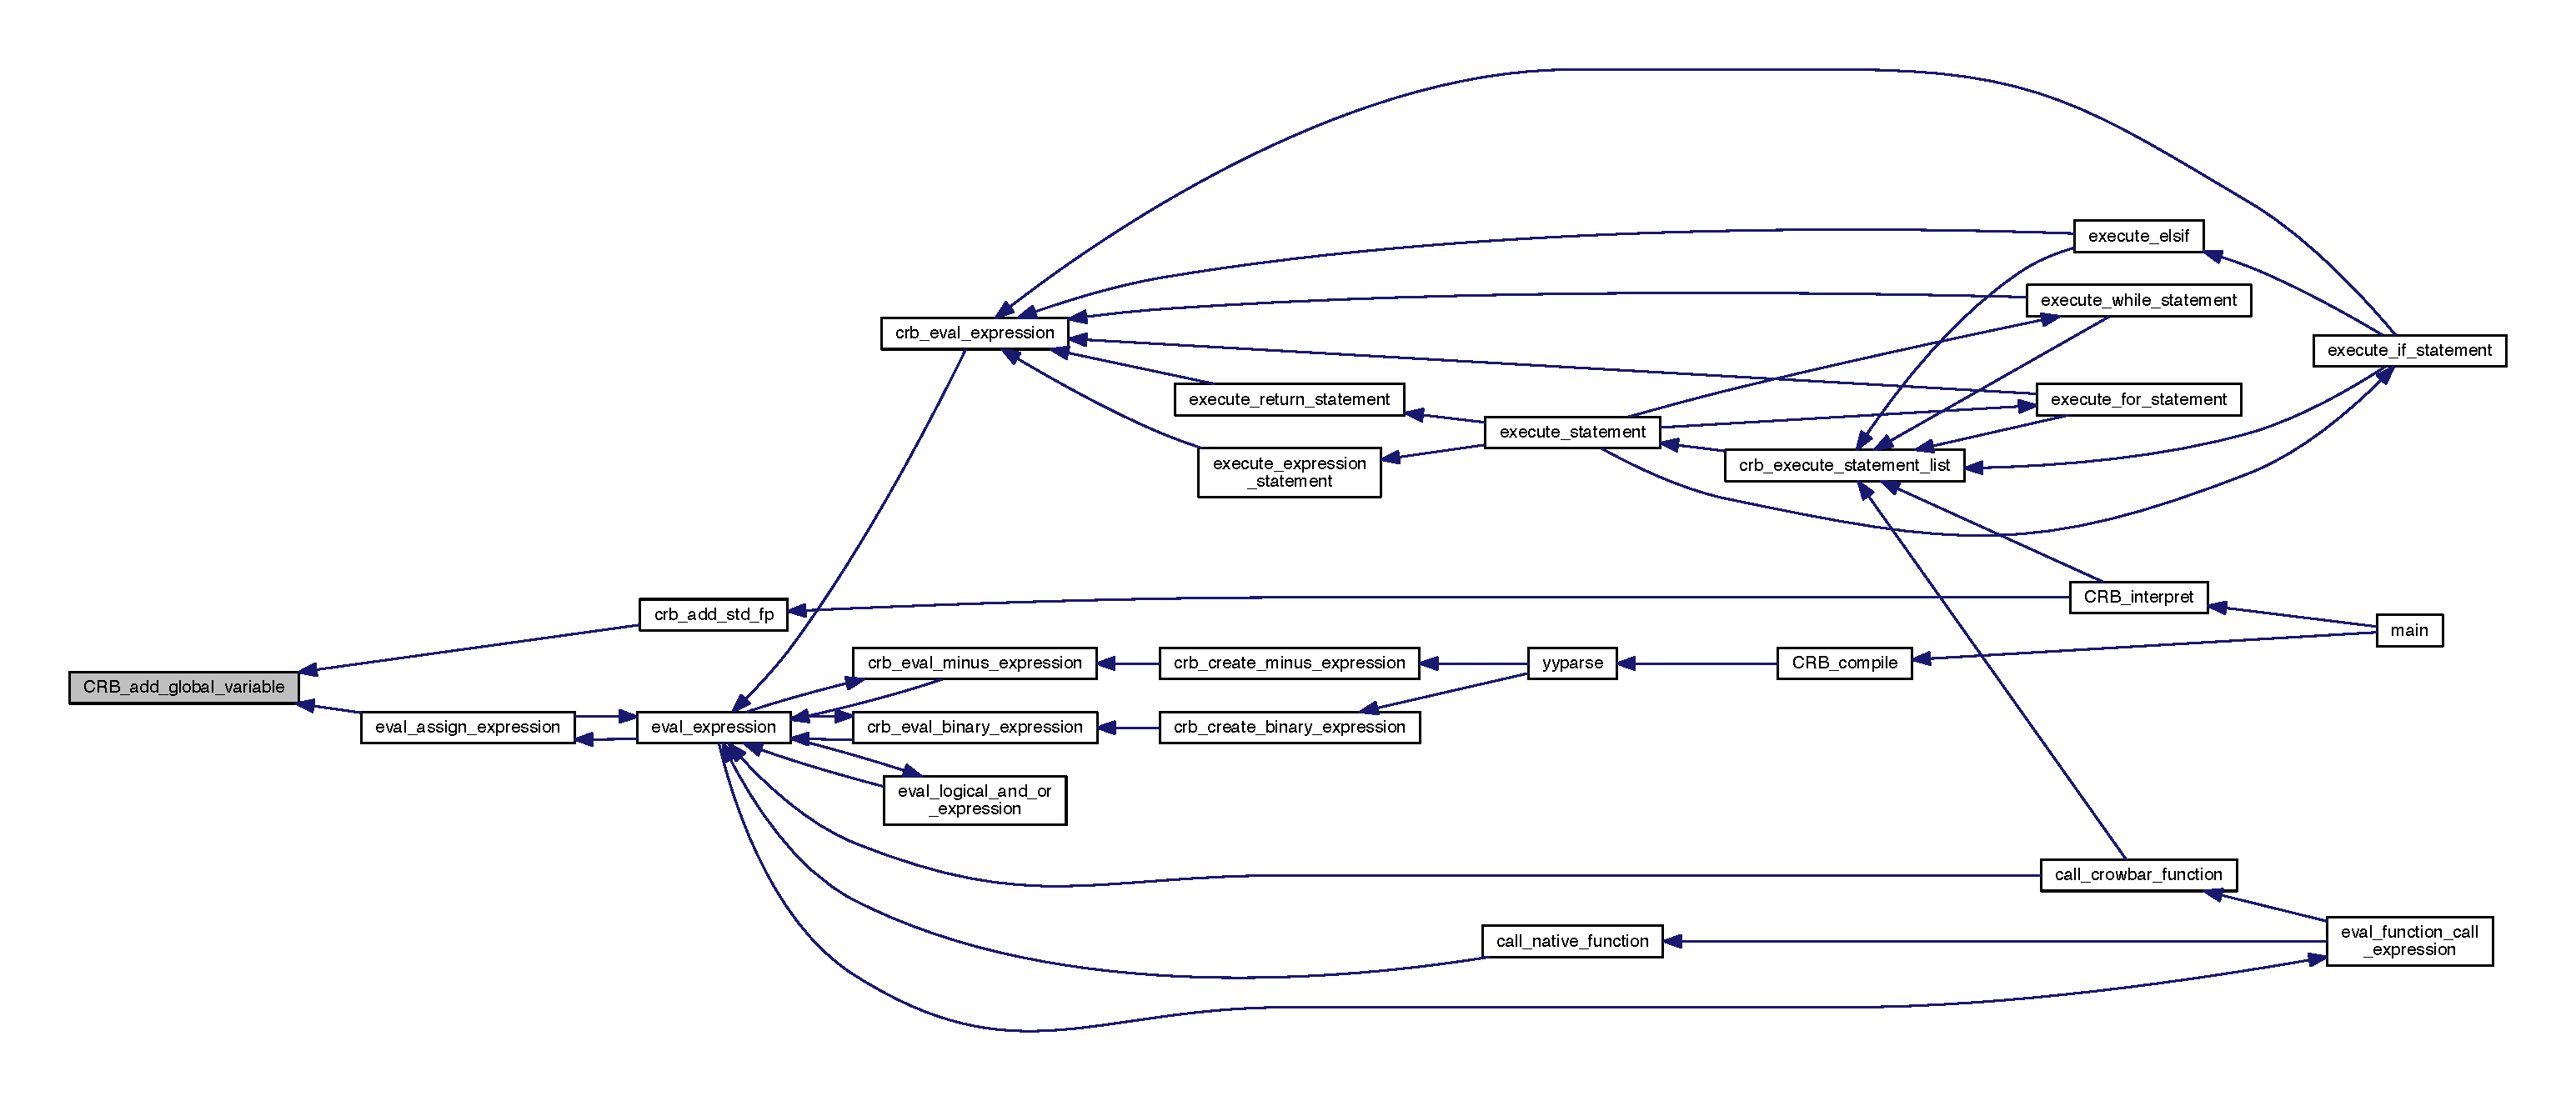
\includegraphics[width=350pt]{_c_r_b__dev_8h_aa4e2d1a292b2c1d9cacba9e06ecdc022_icgraph}
\end{center}
\end{figure}


\hypertarget{_c_r_b__dev_8h_a940149828fe093b31374c316022a981a}{}\index{C\+R\+B\+\_\+dev.\+h@{C\+R\+B\+\_\+dev.\+h}!C\+R\+B\+\_\+add\+\_\+native\+\_\+function@{C\+R\+B\+\_\+add\+\_\+native\+\_\+function}}
\index{C\+R\+B\+\_\+add\+\_\+native\+\_\+function@{C\+R\+B\+\_\+add\+\_\+native\+\_\+function}!C\+R\+B\+\_\+dev.\+h@{C\+R\+B\+\_\+dev.\+h}}
\subsubsection[{C\+R\+B\+\_\+add\+\_\+native\+\_\+function(\+C\+R\+B\+\_\+\+Interpreter $\ast$interpreter, char $\ast$name, C\+R\+B\+\_\+\+Native\+Function\+Proc $\ast$proc)}]{\setlength{\rightskip}{0pt plus 5cm}void C\+R\+B\+\_\+add\+\_\+native\+\_\+function (
\begin{DoxyParamCaption}
\item[{{\bf C\+R\+B\+\_\+\+Interpreter} $\ast$}]{interpreter, }
\item[{char $\ast$}]{name, }
\item[{{\bf C\+R\+B\+\_\+\+Native\+Function\+Proc} $\ast$}]{proc}
\end{DoxyParamCaption}
)}\label{_c_r_b__dev_8h_a940149828fe093b31374c316022a981a}


Here is the call graph for this function\+:\nopagebreak
\begin{figure}[H]
\begin{center}
\leavevmode
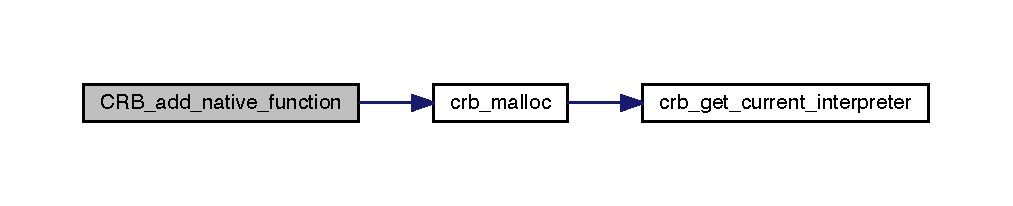
\includegraphics[width=350pt]{_c_r_b__dev_8h_a940149828fe093b31374c316022a981a_cgraph}
\end{center}
\end{figure}




Here is the caller graph for this function\+:
\nopagebreak
\begin{figure}[H]
\begin{center}
\leavevmode
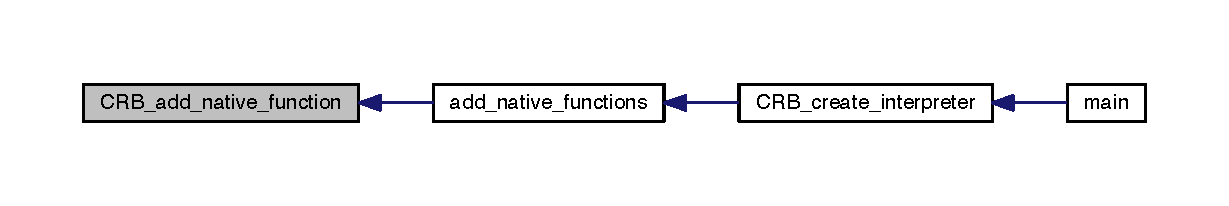
\includegraphics[width=350pt]{_c_r_b__dev_8h_a940149828fe093b31374c316022a981a_icgraph}
\end{center}
\end{figure}



\hypertarget{create_8c}{}\section{create.\+c File Reference}
\label{create_8c}\index{create.\+c@{create.\+c}}
{\ttfamily \#include \char`\"{}M\+E\+M.\+h\char`\"{}}\\*
{\ttfamily \#include \char`\"{}D\+B\+G.\+h\char`\"{}}\\*
{\ttfamily \#include \char`\"{}crowbar.\+h\char`\"{}}\\*
Include dependency graph for create.\+c\+:\nopagebreak
\begin{figure}[H]
\begin{center}
\leavevmode
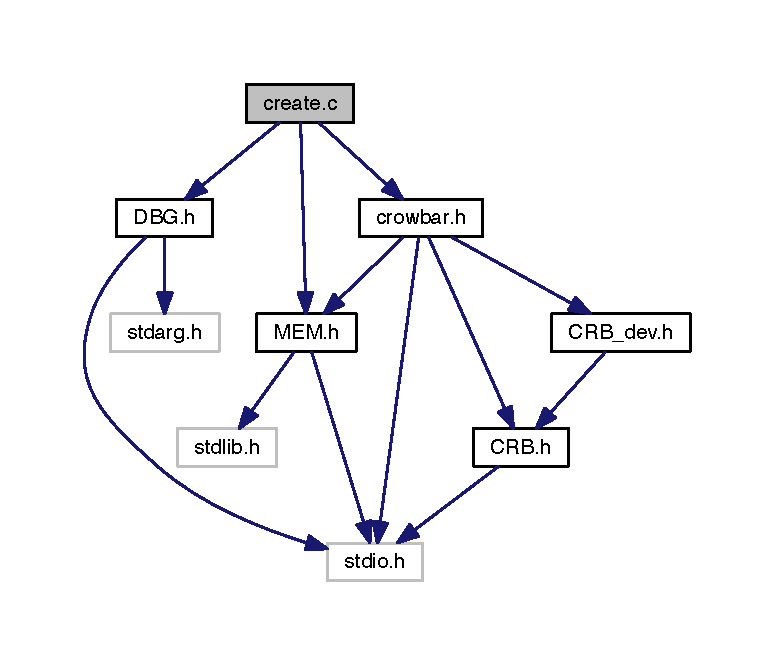
\includegraphics[width=350pt]{create_8c__incl}
\end{center}
\end{figure}
\subsection*{Functions}
\begin{DoxyCompactItemize}
\item 
void \hyperlink{create_8c_aab4b12e9f50a59ecdb6a6201833ff026}{crb\+\_\+function\+\_\+define} (char $\ast$identifier, \hyperlink{crowbar_8h_a7e7687e26b28e339ebcc8eaab571dcf7}{Parameter\+List} $\ast$parameter\+\_\+list, \hyperlink{struct_block}{Block} $\ast$block)
\item 
\hyperlink{crowbar_8h_a7e7687e26b28e339ebcc8eaab571dcf7}{Parameter\+List} $\ast$ \hyperlink{create_8c_a59bf5b154777e78f330ced1c3049574b}{crb\+\_\+create\+\_\+parameter} (char $\ast$identifier)
\item 
\hyperlink{crowbar_8h_a7e7687e26b28e339ebcc8eaab571dcf7}{Parameter\+List} $\ast$ \hyperlink{create_8c_aebfeaf3aaf0402b85db828eb0f7f0595}{crb\+\_\+chain\+\_\+parameter} (\hyperlink{crowbar_8h_a7e7687e26b28e339ebcc8eaab571dcf7}{Parameter\+List} $\ast$list, char $\ast$identifier)
\item 
\hyperlink{crowbar_8h_ad4ba12ca8ae3ead90081fb0aba63aff3}{Argument\+List} $\ast$ \hyperlink{create_8c_ae96ba65b7477930c54d92490049adf18}{crb\+\_\+create\+\_\+argument\+\_\+list} (\hyperlink{crowbar_8h_a070c6feb370aad8a9665ca315bf6ed4a}{Expression} $\ast$expression)
\item 
\hyperlink{crowbar_8h_ad4ba12ca8ae3ead90081fb0aba63aff3}{Argument\+List} $\ast$ \hyperlink{create_8c_ae8c59ecce88d4a70f849a86e10b242c9}{crb\+\_\+chain\+\_\+argument\+\_\+list} (\hyperlink{crowbar_8h_ad4ba12ca8ae3ead90081fb0aba63aff3}{Argument\+List} $\ast$list, \hyperlink{crowbar_8h_a070c6feb370aad8a9665ca315bf6ed4a}{Expression} $\ast$expr)
\item 
\hyperlink{crowbar_8h_a8bffae51ec8146f480c3c14c61b4ff93}{Statement\+List} $\ast$ \hyperlink{create_8c_a43c7c95f8d47ddbe1c6d2408af7ccae6}{crb\+\_\+create\+\_\+statement\+\_\+list} (\hyperlink{crowbar_8h_a16fe74a7a87df7652e815d139b3349d2}{Statement} $\ast$statement)
\item 
\hyperlink{crowbar_8h_a8bffae51ec8146f480c3c14c61b4ff93}{Statement\+List} $\ast$ \hyperlink{create_8c_a1018738c32e8addd8c5cb5c6051b8687}{crb\+\_\+chain\+\_\+statement\+\_\+list} (\hyperlink{crowbar_8h_a8bffae51ec8146f480c3c14c61b4ff93}{Statement\+List} $\ast$list, \hyperlink{crowbar_8h_a16fe74a7a87df7652e815d139b3349d2}{Statement} $\ast$statement)
\item 
\hyperlink{crowbar_8h_a070c6feb370aad8a9665ca315bf6ed4a}{Expression} $\ast$ \hyperlink{create_8c_a3abeb29a324d67cbff71c6383a51ecff}{crb\+\_\+alloc\+\_\+expression} (\hyperlink{crowbar_8h_a51ad9989dafb48362f7e9354d68fe720}{Expression\+Type} type)
\item 
\hyperlink{crowbar_8h_a070c6feb370aad8a9665ca315bf6ed4a}{Expression} $\ast$ \hyperlink{create_8c_ab9772fa63e81db60a419a4e32b6b506a}{crb\+\_\+create\+\_\+assign\+\_\+expression} (char $\ast$variable, \hyperlink{crowbar_8h_a070c6feb370aad8a9665ca315bf6ed4a}{Expression} $\ast$operand)
\item 
static \hyperlink{crowbar_8h_a070c6feb370aad8a9665ca315bf6ed4a}{Expression} \hyperlink{create_8c_abe7f7960e9dd9a45e36f9e032035b0fe}{convert\+\_\+value\+\_\+to\+\_\+expression} (\hyperlink{struct_c_r_b___value}{C\+R\+B\+\_\+\+Value} $\ast$v)
\item 
\hyperlink{crowbar_8h_a070c6feb370aad8a9665ca315bf6ed4a}{Expression} $\ast$ \hyperlink{create_8c_a26c03201a682aa9b1f0e0db5f61e0ddf}{crb\+\_\+create\+\_\+binary\+\_\+expression} (\hyperlink{crowbar_8h_a51ad9989dafb48362f7e9354d68fe720}{Expression\+Type} operator, \hyperlink{crowbar_8h_a070c6feb370aad8a9665ca315bf6ed4a}{Expression} $\ast$left, \hyperlink{crowbar_8h_a070c6feb370aad8a9665ca315bf6ed4a}{Expression} $\ast$right)
\item 
\hyperlink{crowbar_8h_a070c6feb370aad8a9665ca315bf6ed4a}{Expression} $\ast$ \hyperlink{create_8c_aca2e9d85fea19c8f0110a2667d228dcd}{crb\+\_\+create\+\_\+minus\+\_\+expression} (\hyperlink{crowbar_8h_a070c6feb370aad8a9665ca315bf6ed4a}{Expression} $\ast$operand)
\item 
\hyperlink{crowbar_8h_a070c6feb370aad8a9665ca315bf6ed4a}{Expression} $\ast$ \hyperlink{create_8c_a85c3e30f626f6ac351a3af7edffbfa7e}{crb\+\_\+create\+\_\+identifier\+\_\+expression} (char $\ast$identifier)
\item 
\hyperlink{crowbar_8h_a070c6feb370aad8a9665ca315bf6ed4a}{Expression} $\ast$ \hyperlink{create_8c_a5a3487494c040fbba56ae8df2cf7d8df}{crb\+\_\+create\+\_\+function\+\_\+call\+\_\+expression} (char $\ast$func\+\_\+name, \hyperlink{crowbar_8h_ad4ba12ca8ae3ead90081fb0aba63aff3}{Argument\+List} $\ast$argument)
\item 
\hyperlink{crowbar_8h_a070c6feb370aad8a9665ca315bf6ed4a}{Expression} $\ast$ \hyperlink{create_8c_af3cd699497c7714a2a83193965d7a9fd}{crb\+\_\+create\+\_\+boolean\+\_\+expression} (\hyperlink{_c_r_b__dev_8h_a5000f2b447c9132c07d7f1cf66134a69}{C\+R\+B\+\_\+\+Boolean} value)
\item 
\hyperlink{crowbar_8h_a070c6feb370aad8a9665ca315bf6ed4a}{Expression} $\ast$ \hyperlink{create_8c_ae9b1f0d84f1e79aab8387ee4b4e5c3d5}{crb\+\_\+create\+\_\+null\+\_\+expression} (void)
\item 
static \hyperlink{crowbar_8h_a16fe74a7a87df7652e815d139b3349d2}{Statement} $\ast$ \hyperlink{create_8c_ae43dfa3943ba550e9ee3ff06a225ccc3}{alloc\+\_\+statement} (\hyperlink{crowbar_8h_a5f5d0dfd807d2356ecc3cdabf71b3d53}{Statement\+Type} type)
\item 
\hyperlink{crowbar_8h_a16fe74a7a87df7652e815d139b3349d2}{Statement} $\ast$ \hyperlink{create_8c_a5c31f8632625e7685c71e62a3313eec9}{crb\+\_\+create\+\_\+global\+\_\+statement} (\hyperlink{crowbar_8h_a3e8fd423ff4b73a7c5d557375f0a8741}{Identifier\+List} $\ast$identifier\+\_\+list)
\item 
\hyperlink{crowbar_8h_a3e8fd423ff4b73a7c5d557375f0a8741}{Identifier\+List} $\ast$ \hyperlink{create_8c_aef13ab93c73899cb56a0976480f9fcee}{crb\+\_\+create\+\_\+global\+\_\+identifier} (char $\ast$identifier)
\item 
\hyperlink{crowbar_8h_a3e8fd423ff4b73a7c5d557375f0a8741}{Identifier\+List} $\ast$ \hyperlink{create_8c_a94204aff835df4d08e56a4056bde861f}{crb\+\_\+chain\+\_\+identifier} (\hyperlink{crowbar_8h_a3e8fd423ff4b73a7c5d557375f0a8741}{Identifier\+List} $\ast$list, char $\ast$identifier)
\item 
\hyperlink{crowbar_8h_a16fe74a7a87df7652e815d139b3349d2}{Statement} $\ast$ \hyperlink{create_8c_a018cc91ca378066f1a551a1a68719d1d}{crb\+\_\+create\+\_\+if\+\_\+statement} (\hyperlink{crowbar_8h_a070c6feb370aad8a9665ca315bf6ed4a}{Expression} $\ast$condition, \hyperlink{struct_block}{Block} $\ast$then\+\_\+block, \hyperlink{crowbar_8h_a8d2ba32155a8a8a5a87e93c564061f1d}{Elsif} $\ast$elsif\+\_\+list, \hyperlink{struct_block}{Block} $\ast$else\+\_\+block)
\item 
\hyperlink{crowbar_8h_a8d2ba32155a8a8a5a87e93c564061f1d}{Elsif} $\ast$ \hyperlink{create_8c_a919db8b02a380d8b42dab1423989452e}{crb\+\_\+chain\+\_\+elsif\+\_\+list} (\hyperlink{crowbar_8h_a8d2ba32155a8a8a5a87e93c564061f1d}{Elsif} $\ast$list, \hyperlink{crowbar_8h_a8d2ba32155a8a8a5a87e93c564061f1d}{Elsif} $\ast$add)
\item 
\hyperlink{crowbar_8h_a8d2ba32155a8a8a5a87e93c564061f1d}{Elsif} $\ast$ \hyperlink{create_8c_a02bae1b716e6a57b513b2f02ccf8173b}{crb\+\_\+create\+\_\+elsif} (\hyperlink{crowbar_8h_a070c6feb370aad8a9665ca315bf6ed4a}{Expression} $\ast$expr, \hyperlink{struct_block}{Block} $\ast$block)
\item 
\hyperlink{crowbar_8h_a16fe74a7a87df7652e815d139b3349d2}{Statement} $\ast$ \hyperlink{create_8c_a2a1fe3376bf9c5516473f02eac1c98db}{crb\+\_\+create\+\_\+while\+\_\+statement} (\hyperlink{crowbar_8h_a070c6feb370aad8a9665ca315bf6ed4a}{Expression} $\ast$condition, \hyperlink{struct_block}{Block} $\ast$block)
\item 
\hyperlink{crowbar_8h_a16fe74a7a87df7652e815d139b3349d2}{Statement} $\ast$ \hyperlink{create_8c_a60bf6e95f9b6cc5d599b5f77bd1daf6d}{crb\+\_\+create\+\_\+for\+\_\+statement} (\hyperlink{crowbar_8h_a070c6feb370aad8a9665ca315bf6ed4a}{Expression} $\ast$init, \hyperlink{crowbar_8h_a070c6feb370aad8a9665ca315bf6ed4a}{Expression} $\ast$cond, \hyperlink{crowbar_8h_a070c6feb370aad8a9665ca315bf6ed4a}{Expression} $\ast$post, \hyperlink{struct_block}{Block} $\ast$block)
\item 
\hyperlink{struct_block}{Block} $\ast$ \hyperlink{create_8c_abe2319cfb79ec510c7cefe64748fcdaf}{crb\+\_\+create\+\_\+block} (\hyperlink{crowbar_8h_a8bffae51ec8146f480c3c14c61b4ff93}{Statement\+List} $\ast$statement\+\_\+list)
\item 
\hyperlink{crowbar_8h_a16fe74a7a87df7652e815d139b3349d2}{Statement} $\ast$ \hyperlink{create_8c_abf390d7fd73007944e727bf36cbaec4c}{crb\+\_\+create\+\_\+expression\+\_\+statement} (\hyperlink{crowbar_8h_a070c6feb370aad8a9665ca315bf6ed4a}{Expression} $\ast$expression)
\item 
\hyperlink{crowbar_8h_a16fe74a7a87df7652e815d139b3349d2}{Statement} $\ast$ \hyperlink{create_8c_a2a395ba31c3b2b6bf031e09e65a060f3}{crb\+\_\+create\+\_\+return\+\_\+statement} (\hyperlink{crowbar_8h_a070c6feb370aad8a9665ca315bf6ed4a}{Expression} $\ast$expression)
\item 
\hyperlink{crowbar_8h_a16fe74a7a87df7652e815d139b3349d2}{Statement} $\ast$ \hyperlink{create_8c_a4955c08c1840c5e95d46ca639d2497f9}{crb\+\_\+create\+\_\+break\+\_\+statement} (void)
\item 
\hyperlink{crowbar_8h_a16fe74a7a87df7652e815d139b3349d2}{Statement} $\ast$ \hyperlink{create_8c_a850b208585e46095529c372c99ae6cf9}{crb\+\_\+create\+\_\+continue\+\_\+statement} (void)
\end{DoxyCompactItemize}


\subsection{Function Documentation}
\hypertarget{create_8c_ae43dfa3943ba550e9ee3ff06a225ccc3}{}\index{create.\+c@{create.\+c}!alloc\+\_\+statement@{alloc\+\_\+statement}}
\index{alloc\+\_\+statement@{alloc\+\_\+statement}!create.\+c@{create.\+c}}
\subsubsection[{alloc\+\_\+statement(\+Statement\+Type type)}]{\setlength{\rightskip}{0pt plus 5cm}static {\bf Statement}$\ast$ alloc\+\_\+statement (
\begin{DoxyParamCaption}
\item[{{\bf Statement\+Type}}]{type}
\end{DoxyParamCaption}
)\hspace{0.3cm}{\ttfamily [static]}}\label{create_8c_ae43dfa3943ba550e9ee3ff06a225ccc3}


Here is the call graph for this function\+:
\nopagebreak
\begin{figure}[H]
\begin{center}
\leavevmode
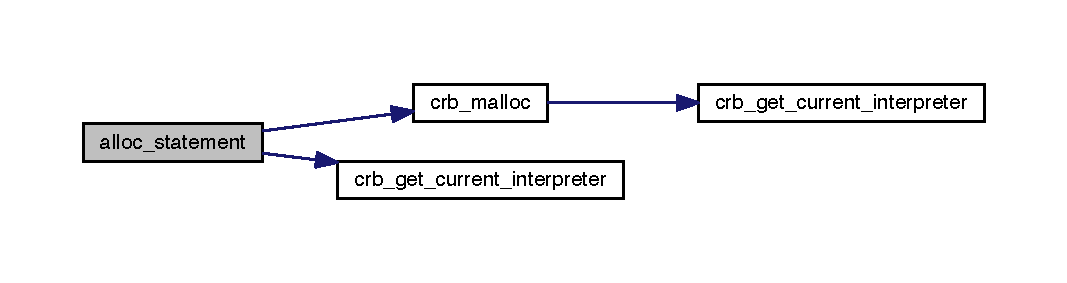
\includegraphics[width=350pt]{create_8c_ae43dfa3943ba550e9ee3ff06a225ccc3_cgraph}
\end{center}
\end{figure}




Here is the caller graph for this function\+:
\nopagebreak
\begin{figure}[H]
\begin{center}
\leavevmode
\includegraphics[width=350pt]{create_8c_ae43dfa3943ba550e9ee3ff06a225ccc3_icgraph}
\end{center}
\end{figure}


\hypertarget{create_8c_abe7f7960e9dd9a45e36f9e032035b0fe}{}\index{create.\+c@{create.\+c}!convert\+\_\+value\+\_\+to\+\_\+expression@{convert\+\_\+value\+\_\+to\+\_\+expression}}
\index{convert\+\_\+value\+\_\+to\+\_\+expression@{convert\+\_\+value\+\_\+to\+\_\+expression}!create.\+c@{create.\+c}}
\subsubsection[{convert\+\_\+value\+\_\+to\+\_\+expression(\+C\+R\+B\+\_\+\+Value $\ast$v)}]{\setlength{\rightskip}{0pt plus 5cm}static {\bf Expression} convert\+\_\+value\+\_\+to\+\_\+expression (
\begin{DoxyParamCaption}
\item[{{\bf C\+R\+B\+\_\+\+Value} $\ast$}]{v}
\end{DoxyParamCaption}
)\hspace{0.3cm}{\ttfamily [static]}}\label{create_8c_abe7f7960e9dd9a45e36f9e032035b0fe}


Here is the caller graph for this function\+:
\nopagebreak
\begin{figure}[H]
\begin{center}
\leavevmode
\includegraphics[width=350pt]{create_8c_abe7f7960e9dd9a45e36f9e032035b0fe_icgraph}
\end{center}
\end{figure}


\hypertarget{create_8c_a3abeb29a324d67cbff71c6383a51ecff}{}\index{create.\+c@{create.\+c}!crb\+\_\+alloc\+\_\+expression@{crb\+\_\+alloc\+\_\+expression}}
\index{crb\+\_\+alloc\+\_\+expression@{crb\+\_\+alloc\+\_\+expression}!create.\+c@{create.\+c}}
\subsubsection[{crb\+\_\+alloc\+\_\+expression(\+Expression\+Type type)}]{\setlength{\rightskip}{0pt plus 5cm}{\bf Expression}$\ast$ crb\+\_\+alloc\+\_\+expression (
\begin{DoxyParamCaption}
\item[{{\bf Expression\+Type}}]{type}
\end{DoxyParamCaption}
)}\label{create_8c_a3abeb29a324d67cbff71c6383a51ecff}


Here is the call graph for this function\+:\nopagebreak
\begin{figure}[H]
\begin{center}
\leavevmode
\includegraphics[width=350pt]{create_8c_a3abeb29a324d67cbff71c6383a51ecff_cgraph}
\end{center}
\end{figure}




Here is the caller graph for this function\+:\nopagebreak
\begin{figure}[H]
\begin{center}
\leavevmode
\includegraphics[width=350pt]{create_8c_a3abeb29a324d67cbff71c6383a51ecff_icgraph}
\end{center}
\end{figure}


\hypertarget{create_8c_ae8c59ecce88d4a70f849a86e10b242c9}{}\index{create.\+c@{create.\+c}!crb\+\_\+chain\+\_\+argument\+\_\+list@{crb\+\_\+chain\+\_\+argument\+\_\+list}}
\index{crb\+\_\+chain\+\_\+argument\+\_\+list@{crb\+\_\+chain\+\_\+argument\+\_\+list}!create.\+c@{create.\+c}}
\subsubsection[{crb\+\_\+chain\+\_\+argument\+\_\+list(\+Argument\+List $\ast$list, Expression $\ast$expr)}]{\setlength{\rightskip}{0pt plus 5cm}{\bf Argument\+List}$\ast$ crb\+\_\+chain\+\_\+argument\+\_\+list (
\begin{DoxyParamCaption}
\item[{{\bf Argument\+List} $\ast$}]{list, }
\item[{{\bf Expression} $\ast$}]{expr}
\end{DoxyParamCaption}
)}\label{create_8c_ae8c59ecce88d4a70f849a86e10b242c9}


Here is the call graph for this function\+:\nopagebreak
\begin{figure}[H]
\begin{center}
\leavevmode
\includegraphics[width=350pt]{create_8c_ae8c59ecce88d4a70f849a86e10b242c9_cgraph}
\end{center}
\end{figure}




Here is the caller graph for this function\+:\nopagebreak
\begin{figure}[H]
\begin{center}
\leavevmode
\includegraphics[width=350pt]{create_8c_ae8c59ecce88d4a70f849a86e10b242c9_icgraph}
\end{center}
\end{figure}


\hypertarget{create_8c_a919db8b02a380d8b42dab1423989452e}{}\index{create.\+c@{create.\+c}!crb\+\_\+chain\+\_\+elsif\+\_\+list@{crb\+\_\+chain\+\_\+elsif\+\_\+list}}
\index{crb\+\_\+chain\+\_\+elsif\+\_\+list@{crb\+\_\+chain\+\_\+elsif\+\_\+list}!create.\+c@{create.\+c}}
\subsubsection[{crb\+\_\+chain\+\_\+elsif\+\_\+list(\+Elsif $\ast$list, Elsif $\ast$add)}]{\setlength{\rightskip}{0pt plus 5cm}{\bf Elsif}$\ast$ crb\+\_\+chain\+\_\+elsif\+\_\+list (
\begin{DoxyParamCaption}
\item[{{\bf Elsif} $\ast$}]{list, }
\item[{{\bf Elsif} $\ast$}]{add}
\end{DoxyParamCaption}
)}\label{create_8c_a919db8b02a380d8b42dab1423989452e}


Here is the caller graph for this function\+:\nopagebreak
\begin{figure}[H]
\begin{center}
\leavevmode
\includegraphics[width=350pt]{create_8c_a919db8b02a380d8b42dab1423989452e_icgraph}
\end{center}
\end{figure}


\hypertarget{create_8c_a94204aff835df4d08e56a4056bde861f}{}\index{create.\+c@{create.\+c}!crb\+\_\+chain\+\_\+identifier@{crb\+\_\+chain\+\_\+identifier}}
\index{crb\+\_\+chain\+\_\+identifier@{crb\+\_\+chain\+\_\+identifier}!create.\+c@{create.\+c}}
\subsubsection[{crb\+\_\+chain\+\_\+identifier(\+Identifier\+List $\ast$list, char $\ast$identifier)}]{\setlength{\rightskip}{0pt plus 5cm}{\bf Identifier\+List}$\ast$ crb\+\_\+chain\+\_\+identifier (
\begin{DoxyParamCaption}
\item[{{\bf Identifier\+List} $\ast$}]{list, }
\item[{char $\ast$}]{identifier}
\end{DoxyParamCaption}
)}\label{create_8c_a94204aff835df4d08e56a4056bde861f}


Here is the call graph for this function\+:\nopagebreak
\begin{figure}[H]
\begin{center}
\leavevmode
\includegraphics[width=350pt]{create_8c_a94204aff835df4d08e56a4056bde861f_cgraph}
\end{center}
\end{figure}




Here is the caller graph for this function\+:\nopagebreak
\begin{figure}[H]
\begin{center}
\leavevmode
\includegraphics[width=350pt]{create_8c_a94204aff835df4d08e56a4056bde861f_icgraph}
\end{center}
\end{figure}


\hypertarget{create_8c_aebfeaf3aaf0402b85db828eb0f7f0595}{}\index{create.\+c@{create.\+c}!crb\+\_\+chain\+\_\+parameter@{crb\+\_\+chain\+\_\+parameter}}
\index{crb\+\_\+chain\+\_\+parameter@{crb\+\_\+chain\+\_\+parameter}!create.\+c@{create.\+c}}
\subsubsection[{crb\+\_\+chain\+\_\+parameter(\+Parameter\+List $\ast$list, char $\ast$identifier)}]{\setlength{\rightskip}{0pt plus 5cm}{\bf Parameter\+List}$\ast$ crb\+\_\+chain\+\_\+parameter (
\begin{DoxyParamCaption}
\item[{{\bf Parameter\+List} $\ast$}]{list, }
\item[{char $\ast$}]{identifier}
\end{DoxyParamCaption}
)}\label{create_8c_aebfeaf3aaf0402b85db828eb0f7f0595}


Here is the call graph for this function\+:\nopagebreak
\begin{figure}[H]
\begin{center}
\leavevmode
\includegraphics[width=350pt]{create_8c_aebfeaf3aaf0402b85db828eb0f7f0595_cgraph}
\end{center}
\end{figure}




Here is the caller graph for this function\+:\nopagebreak
\begin{figure}[H]
\begin{center}
\leavevmode
\includegraphics[width=350pt]{create_8c_aebfeaf3aaf0402b85db828eb0f7f0595_icgraph}
\end{center}
\end{figure}


\hypertarget{create_8c_a1018738c32e8addd8c5cb5c6051b8687}{}\index{create.\+c@{create.\+c}!crb\+\_\+chain\+\_\+statement\+\_\+list@{crb\+\_\+chain\+\_\+statement\+\_\+list}}
\index{crb\+\_\+chain\+\_\+statement\+\_\+list@{crb\+\_\+chain\+\_\+statement\+\_\+list}!create.\+c@{create.\+c}}
\subsubsection[{crb\+\_\+chain\+\_\+statement\+\_\+list(\+Statement\+List $\ast$list, Statement $\ast$statement)}]{\setlength{\rightskip}{0pt plus 5cm}{\bf Statement\+List}$\ast$ crb\+\_\+chain\+\_\+statement\+\_\+list (
\begin{DoxyParamCaption}
\item[{{\bf Statement\+List} $\ast$}]{list, }
\item[{{\bf Statement} $\ast$}]{statement}
\end{DoxyParamCaption}
)}\label{create_8c_a1018738c32e8addd8c5cb5c6051b8687}


Here is the call graph for this function\+:\nopagebreak
\begin{figure}[H]
\begin{center}
\leavevmode
\includegraphics[width=350pt]{create_8c_a1018738c32e8addd8c5cb5c6051b8687_cgraph}
\end{center}
\end{figure}




Here is the caller graph for this function\+:\nopagebreak
\begin{figure}[H]
\begin{center}
\leavevmode
\includegraphics[width=350pt]{create_8c_a1018738c32e8addd8c5cb5c6051b8687_icgraph}
\end{center}
\end{figure}


\hypertarget{create_8c_ae96ba65b7477930c54d92490049adf18}{}\index{create.\+c@{create.\+c}!crb\+\_\+create\+\_\+argument\+\_\+list@{crb\+\_\+create\+\_\+argument\+\_\+list}}
\index{crb\+\_\+create\+\_\+argument\+\_\+list@{crb\+\_\+create\+\_\+argument\+\_\+list}!create.\+c@{create.\+c}}
\subsubsection[{crb\+\_\+create\+\_\+argument\+\_\+list(\+Expression $\ast$expression)}]{\setlength{\rightskip}{0pt plus 5cm}{\bf Argument\+List}$\ast$ crb\+\_\+create\+\_\+argument\+\_\+list (
\begin{DoxyParamCaption}
\item[{{\bf Expression} $\ast$}]{expression}
\end{DoxyParamCaption}
)}\label{create_8c_ae96ba65b7477930c54d92490049adf18}


Here is the call graph for this function\+:\nopagebreak
\begin{figure}[H]
\begin{center}
\leavevmode
\includegraphics[width=350pt]{create_8c_ae96ba65b7477930c54d92490049adf18_cgraph}
\end{center}
\end{figure}




Here is the caller graph for this function\+:\nopagebreak
\begin{figure}[H]
\begin{center}
\leavevmode
\includegraphics[width=350pt]{create_8c_ae96ba65b7477930c54d92490049adf18_icgraph}
\end{center}
\end{figure}


\hypertarget{create_8c_ab9772fa63e81db60a419a4e32b6b506a}{}\index{create.\+c@{create.\+c}!crb\+\_\+create\+\_\+assign\+\_\+expression@{crb\+\_\+create\+\_\+assign\+\_\+expression}}
\index{crb\+\_\+create\+\_\+assign\+\_\+expression@{crb\+\_\+create\+\_\+assign\+\_\+expression}!create.\+c@{create.\+c}}
\subsubsection[{crb\+\_\+create\+\_\+assign\+\_\+expression(char $\ast$variable, Expression $\ast$operand)}]{\setlength{\rightskip}{0pt plus 5cm}{\bf Expression}$\ast$ crb\+\_\+create\+\_\+assign\+\_\+expression (
\begin{DoxyParamCaption}
\item[{char $\ast$}]{variable, }
\item[{{\bf Expression} $\ast$}]{operand}
\end{DoxyParamCaption}
)}\label{create_8c_ab9772fa63e81db60a419a4e32b6b506a}


Here is the call graph for this function\+:\nopagebreak
\begin{figure}[H]
\begin{center}
\leavevmode
\includegraphics[width=350pt]{create_8c_ab9772fa63e81db60a419a4e32b6b506a_cgraph}
\end{center}
\end{figure}




Here is the caller graph for this function\+:\nopagebreak
\begin{figure}[H]
\begin{center}
\leavevmode
\includegraphics[width=350pt]{create_8c_ab9772fa63e81db60a419a4e32b6b506a_icgraph}
\end{center}
\end{figure}


\hypertarget{create_8c_a26c03201a682aa9b1f0e0db5f61e0ddf}{}\index{create.\+c@{create.\+c}!crb\+\_\+create\+\_\+binary\+\_\+expression@{crb\+\_\+create\+\_\+binary\+\_\+expression}}
\index{crb\+\_\+create\+\_\+binary\+\_\+expression@{crb\+\_\+create\+\_\+binary\+\_\+expression}!create.\+c@{create.\+c}}
\subsubsection[{crb\+\_\+create\+\_\+binary\+\_\+expression(\+Expression\+Type operator, Expression $\ast$left, Expression $\ast$right)}]{\setlength{\rightskip}{0pt plus 5cm}{\bf Expression}$\ast$ crb\+\_\+create\+\_\+binary\+\_\+expression (
\begin{DoxyParamCaption}
\item[{{\bf Expression\+Type}}]{operator, }
\item[{{\bf Expression} $\ast$}]{left, }
\item[{{\bf Expression} $\ast$}]{right}
\end{DoxyParamCaption}
)}\label{create_8c_a26c03201a682aa9b1f0e0db5f61e0ddf}


Here is the call graph for this function\+:
\nopagebreak
\begin{figure}[H]
\begin{center}
\leavevmode
\includegraphics[width=350pt]{create_8c_a26c03201a682aa9b1f0e0db5f61e0ddf_cgraph}
\end{center}
\end{figure}




Here is the caller graph for this function\+:\nopagebreak
\begin{figure}[H]
\begin{center}
\leavevmode
\includegraphics[width=350pt]{create_8c_a26c03201a682aa9b1f0e0db5f61e0ddf_icgraph}
\end{center}
\end{figure}


\hypertarget{create_8c_abe2319cfb79ec510c7cefe64748fcdaf}{}\index{create.\+c@{create.\+c}!crb\+\_\+create\+\_\+block@{crb\+\_\+create\+\_\+block}}
\index{crb\+\_\+create\+\_\+block@{crb\+\_\+create\+\_\+block}!create.\+c@{create.\+c}}
\subsubsection[{crb\+\_\+create\+\_\+block(\+Statement\+List $\ast$statement\+\_\+list)}]{\setlength{\rightskip}{0pt plus 5cm}{\bf Block}$\ast$ crb\+\_\+create\+\_\+block (
\begin{DoxyParamCaption}
\item[{{\bf Statement\+List} $\ast$}]{statement\+\_\+list}
\end{DoxyParamCaption}
)}\label{create_8c_abe2319cfb79ec510c7cefe64748fcdaf}


Here is the call graph for this function\+:\nopagebreak
\begin{figure}[H]
\begin{center}
\leavevmode
\includegraphics[width=350pt]{create_8c_abe2319cfb79ec510c7cefe64748fcdaf_cgraph}
\end{center}
\end{figure}




Here is the caller graph for this function\+:\nopagebreak
\begin{figure}[H]
\begin{center}
\leavevmode
\includegraphics[width=350pt]{create_8c_abe2319cfb79ec510c7cefe64748fcdaf_icgraph}
\end{center}
\end{figure}


\hypertarget{create_8c_af3cd699497c7714a2a83193965d7a9fd}{}\index{create.\+c@{create.\+c}!crb\+\_\+create\+\_\+boolean\+\_\+expression@{crb\+\_\+create\+\_\+boolean\+\_\+expression}}
\index{crb\+\_\+create\+\_\+boolean\+\_\+expression@{crb\+\_\+create\+\_\+boolean\+\_\+expression}!create.\+c@{create.\+c}}
\subsubsection[{crb\+\_\+create\+\_\+boolean\+\_\+expression(\+C\+R\+B\+\_\+\+Boolean value)}]{\setlength{\rightskip}{0pt plus 5cm}{\bf Expression}$\ast$ crb\+\_\+create\+\_\+boolean\+\_\+expression (
\begin{DoxyParamCaption}
\item[{{\bf C\+R\+B\+\_\+\+Boolean}}]{value}
\end{DoxyParamCaption}
)}\label{create_8c_af3cd699497c7714a2a83193965d7a9fd}


Here is the call graph for this function\+:\nopagebreak
\begin{figure}[H]
\begin{center}
\leavevmode
\includegraphics[width=350pt]{create_8c_af3cd699497c7714a2a83193965d7a9fd_cgraph}
\end{center}
\end{figure}




Here is the caller graph for this function\+:\nopagebreak
\begin{figure}[H]
\begin{center}
\leavevmode
\includegraphics[width=350pt]{create_8c_af3cd699497c7714a2a83193965d7a9fd_icgraph}
\end{center}
\end{figure}


\hypertarget{create_8c_a4955c08c1840c5e95d46ca639d2497f9}{}\index{create.\+c@{create.\+c}!crb\+\_\+create\+\_\+break\+\_\+statement@{crb\+\_\+create\+\_\+break\+\_\+statement}}
\index{crb\+\_\+create\+\_\+break\+\_\+statement@{crb\+\_\+create\+\_\+break\+\_\+statement}!create.\+c@{create.\+c}}
\subsubsection[{crb\+\_\+create\+\_\+break\+\_\+statement(void)}]{\setlength{\rightskip}{0pt plus 5cm}{\bf Statement}$\ast$ crb\+\_\+create\+\_\+break\+\_\+statement (
\begin{DoxyParamCaption}
\item[{void}]{}
\end{DoxyParamCaption}
)}\label{create_8c_a4955c08c1840c5e95d46ca639d2497f9}


Here is the call graph for this function\+:
\nopagebreak
\begin{figure}[H]
\begin{center}
\leavevmode
\includegraphics[width=350pt]{create_8c_a4955c08c1840c5e95d46ca639d2497f9_cgraph}
\end{center}
\end{figure}




Here is the caller graph for this function\+:\nopagebreak
\begin{figure}[H]
\begin{center}
\leavevmode
\includegraphics[width=350pt]{create_8c_a4955c08c1840c5e95d46ca639d2497f9_icgraph}
\end{center}
\end{figure}


\hypertarget{create_8c_a850b208585e46095529c372c99ae6cf9}{}\index{create.\+c@{create.\+c}!crb\+\_\+create\+\_\+continue\+\_\+statement@{crb\+\_\+create\+\_\+continue\+\_\+statement}}
\index{crb\+\_\+create\+\_\+continue\+\_\+statement@{crb\+\_\+create\+\_\+continue\+\_\+statement}!create.\+c@{create.\+c}}
\subsubsection[{crb\+\_\+create\+\_\+continue\+\_\+statement(void)}]{\setlength{\rightskip}{0pt plus 5cm}{\bf Statement}$\ast$ crb\+\_\+create\+\_\+continue\+\_\+statement (
\begin{DoxyParamCaption}
\item[{void}]{}
\end{DoxyParamCaption}
)}\label{create_8c_a850b208585e46095529c372c99ae6cf9}


Here is the call graph for this function\+:
\nopagebreak
\begin{figure}[H]
\begin{center}
\leavevmode
\includegraphics[width=350pt]{create_8c_a850b208585e46095529c372c99ae6cf9_cgraph}
\end{center}
\end{figure}




Here is the caller graph for this function\+:\nopagebreak
\begin{figure}[H]
\begin{center}
\leavevmode
\includegraphics[width=350pt]{create_8c_a850b208585e46095529c372c99ae6cf9_icgraph}
\end{center}
\end{figure}


\hypertarget{create_8c_a02bae1b716e6a57b513b2f02ccf8173b}{}\index{create.\+c@{create.\+c}!crb\+\_\+create\+\_\+elsif@{crb\+\_\+create\+\_\+elsif}}
\index{crb\+\_\+create\+\_\+elsif@{crb\+\_\+create\+\_\+elsif}!create.\+c@{create.\+c}}
\subsubsection[{crb\+\_\+create\+\_\+elsif(\+Expression $\ast$expr, Block $\ast$block)}]{\setlength{\rightskip}{0pt plus 5cm}{\bf Elsif}$\ast$ crb\+\_\+create\+\_\+elsif (
\begin{DoxyParamCaption}
\item[{{\bf Expression} $\ast$}]{expr, }
\item[{{\bf Block} $\ast$}]{block}
\end{DoxyParamCaption}
)}\label{create_8c_a02bae1b716e6a57b513b2f02ccf8173b}


Here is the call graph for this function\+:\nopagebreak
\begin{figure}[H]
\begin{center}
\leavevmode
\includegraphics[width=350pt]{create_8c_a02bae1b716e6a57b513b2f02ccf8173b_cgraph}
\end{center}
\end{figure}




Here is the caller graph for this function\+:\nopagebreak
\begin{figure}[H]
\begin{center}
\leavevmode
\includegraphics[width=350pt]{create_8c_a02bae1b716e6a57b513b2f02ccf8173b_icgraph}
\end{center}
\end{figure}


\hypertarget{create_8c_abf390d7fd73007944e727bf36cbaec4c}{}\index{create.\+c@{create.\+c}!crb\+\_\+create\+\_\+expression\+\_\+statement@{crb\+\_\+create\+\_\+expression\+\_\+statement}}
\index{crb\+\_\+create\+\_\+expression\+\_\+statement@{crb\+\_\+create\+\_\+expression\+\_\+statement}!create.\+c@{create.\+c}}
\subsubsection[{crb\+\_\+create\+\_\+expression\+\_\+statement(\+Expression $\ast$expression)}]{\setlength{\rightskip}{0pt plus 5cm}{\bf Statement}$\ast$ crb\+\_\+create\+\_\+expression\+\_\+statement (
\begin{DoxyParamCaption}
\item[{{\bf Expression} $\ast$}]{expression}
\end{DoxyParamCaption}
)}\label{create_8c_abf390d7fd73007944e727bf36cbaec4c}


Here is the call graph for this function\+:
\nopagebreak
\begin{figure}[H]
\begin{center}
\leavevmode
\includegraphics[width=350pt]{create_8c_abf390d7fd73007944e727bf36cbaec4c_cgraph}
\end{center}
\end{figure}




Here is the caller graph for this function\+:\nopagebreak
\begin{figure}[H]
\begin{center}
\leavevmode
\includegraphics[width=350pt]{create_8c_abf390d7fd73007944e727bf36cbaec4c_icgraph}
\end{center}
\end{figure}


\hypertarget{create_8c_a60bf6e95f9b6cc5d599b5f77bd1daf6d}{}\index{create.\+c@{create.\+c}!crb\+\_\+create\+\_\+for\+\_\+statement@{crb\+\_\+create\+\_\+for\+\_\+statement}}
\index{crb\+\_\+create\+\_\+for\+\_\+statement@{crb\+\_\+create\+\_\+for\+\_\+statement}!create.\+c@{create.\+c}}
\subsubsection[{crb\+\_\+create\+\_\+for\+\_\+statement(\+Expression $\ast$init, Expression $\ast$cond, Expression $\ast$post, Block $\ast$block)}]{\setlength{\rightskip}{0pt plus 5cm}{\bf Statement}$\ast$ crb\+\_\+create\+\_\+for\+\_\+statement (
\begin{DoxyParamCaption}
\item[{{\bf Expression} $\ast$}]{init, }
\item[{{\bf Expression} $\ast$}]{cond, }
\item[{{\bf Expression} $\ast$}]{post, }
\item[{{\bf Block} $\ast$}]{block}
\end{DoxyParamCaption}
)}\label{create_8c_a60bf6e95f9b6cc5d599b5f77bd1daf6d}


Here is the call graph for this function\+:
\nopagebreak
\begin{figure}[H]
\begin{center}
\leavevmode
\includegraphics[width=350pt]{create_8c_a60bf6e95f9b6cc5d599b5f77bd1daf6d_cgraph}
\end{center}
\end{figure}




Here is the caller graph for this function\+:\nopagebreak
\begin{figure}[H]
\begin{center}
\leavevmode
\includegraphics[width=350pt]{create_8c_a60bf6e95f9b6cc5d599b5f77bd1daf6d_icgraph}
\end{center}
\end{figure}


\hypertarget{create_8c_a5a3487494c040fbba56ae8df2cf7d8df}{}\index{create.\+c@{create.\+c}!crb\+\_\+create\+\_\+function\+\_\+call\+\_\+expression@{crb\+\_\+create\+\_\+function\+\_\+call\+\_\+expression}}
\index{crb\+\_\+create\+\_\+function\+\_\+call\+\_\+expression@{crb\+\_\+create\+\_\+function\+\_\+call\+\_\+expression}!create.\+c@{create.\+c}}
\subsubsection[{crb\+\_\+create\+\_\+function\+\_\+call\+\_\+expression(char $\ast$func\+\_\+name, Argument\+List $\ast$argument)}]{\setlength{\rightskip}{0pt plus 5cm}{\bf Expression}$\ast$ crb\+\_\+create\+\_\+function\+\_\+call\+\_\+expression (
\begin{DoxyParamCaption}
\item[{char $\ast$}]{func\+\_\+name, }
\item[{{\bf Argument\+List} $\ast$}]{argument}
\end{DoxyParamCaption}
)}\label{create_8c_a5a3487494c040fbba56ae8df2cf7d8df}


Here is the call graph for this function\+:\nopagebreak
\begin{figure}[H]
\begin{center}
\leavevmode
\includegraphics[width=350pt]{create_8c_a5a3487494c040fbba56ae8df2cf7d8df_cgraph}
\end{center}
\end{figure}




Here is the caller graph for this function\+:\nopagebreak
\begin{figure}[H]
\begin{center}
\leavevmode
\includegraphics[width=350pt]{create_8c_a5a3487494c040fbba56ae8df2cf7d8df_icgraph}
\end{center}
\end{figure}


\hypertarget{create_8c_aef13ab93c73899cb56a0976480f9fcee}{}\index{create.\+c@{create.\+c}!crb\+\_\+create\+\_\+global\+\_\+identifier@{crb\+\_\+create\+\_\+global\+\_\+identifier}}
\index{crb\+\_\+create\+\_\+global\+\_\+identifier@{crb\+\_\+create\+\_\+global\+\_\+identifier}!create.\+c@{create.\+c}}
\subsubsection[{crb\+\_\+create\+\_\+global\+\_\+identifier(char $\ast$identifier)}]{\setlength{\rightskip}{0pt plus 5cm}{\bf Identifier\+List}$\ast$ crb\+\_\+create\+\_\+global\+\_\+identifier (
\begin{DoxyParamCaption}
\item[{char $\ast$}]{identifier}
\end{DoxyParamCaption}
)}\label{create_8c_aef13ab93c73899cb56a0976480f9fcee}


Here is the call graph for this function\+:\nopagebreak
\begin{figure}[H]
\begin{center}
\leavevmode
\includegraphics[width=350pt]{create_8c_aef13ab93c73899cb56a0976480f9fcee_cgraph}
\end{center}
\end{figure}




Here is the caller graph for this function\+:\nopagebreak
\begin{figure}[H]
\begin{center}
\leavevmode
\includegraphics[width=350pt]{create_8c_aef13ab93c73899cb56a0976480f9fcee_icgraph}
\end{center}
\end{figure}


\hypertarget{create_8c_a5c31f8632625e7685c71e62a3313eec9}{}\index{create.\+c@{create.\+c}!crb\+\_\+create\+\_\+global\+\_\+statement@{crb\+\_\+create\+\_\+global\+\_\+statement}}
\index{crb\+\_\+create\+\_\+global\+\_\+statement@{crb\+\_\+create\+\_\+global\+\_\+statement}!create.\+c@{create.\+c}}
\subsubsection[{crb\+\_\+create\+\_\+global\+\_\+statement(\+Identifier\+List $\ast$identifier\+\_\+list)}]{\setlength{\rightskip}{0pt plus 5cm}{\bf Statement}$\ast$ crb\+\_\+create\+\_\+global\+\_\+statement (
\begin{DoxyParamCaption}
\item[{{\bf Identifier\+List} $\ast$}]{identifier\+\_\+list}
\end{DoxyParamCaption}
)}\label{create_8c_a5c31f8632625e7685c71e62a3313eec9}


Here is the call graph for this function\+:
\nopagebreak
\begin{figure}[H]
\begin{center}
\leavevmode
\includegraphics[width=350pt]{create_8c_a5c31f8632625e7685c71e62a3313eec9_cgraph}
\end{center}
\end{figure}




Here is the caller graph for this function\+:\nopagebreak
\begin{figure}[H]
\begin{center}
\leavevmode
\includegraphics[width=350pt]{create_8c_a5c31f8632625e7685c71e62a3313eec9_icgraph}
\end{center}
\end{figure}


\hypertarget{create_8c_a85c3e30f626f6ac351a3af7edffbfa7e}{}\index{create.\+c@{create.\+c}!crb\+\_\+create\+\_\+identifier\+\_\+expression@{crb\+\_\+create\+\_\+identifier\+\_\+expression}}
\index{crb\+\_\+create\+\_\+identifier\+\_\+expression@{crb\+\_\+create\+\_\+identifier\+\_\+expression}!create.\+c@{create.\+c}}
\subsubsection[{crb\+\_\+create\+\_\+identifier\+\_\+expression(char $\ast$identifier)}]{\setlength{\rightskip}{0pt plus 5cm}{\bf Expression}$\ast$ crb\+\_\+create\+\_\+identifier\+\_\+expression (
\begin{DoxyParamCaption}
\item[{char $\ast$}]{identifier}
\end{DoxyParamCaption}
)}\label{create_8c_a85c3e30f626f6ac351a3af7edffbfa7e}


Here is the call graph for this function\+:\nopagebreak
\begin{figure}[H]
\begin{center}
\leavevmode
\includegraphics[width=350pt]{create_8c_a85c3e30f626f6ac351a3af7edffbfa7e_cgraph}
\end{center}
\end{figure}




Here is the caller graph for this function\+:\nopagebreak
\begin{figure}[H]
\begin{center}
\leavevmode
\includegraphics[width=350pt]{create_8c_a85c3e30f626f6ac351a3af7edffbfa7e_icgraph}
\end{center}
\end{figure}


\hypertarget{create_8c_a018cc91ca378066f1a551a1a68719d1d}{}\index{create.\+c@{create.\+c}!crb\+\_\+create\+\_\+if\+\_\+statement@{crb\+\_\+create\+\_\+if\+\_\+statement}}
\index{crb\+\_\+create\+\_\+if\+\_\+statement@{crb\+\_\+create\+\_\+if\+\_\+statement}!create.\+c@{create.\+c}}
\subsubsection[{crb\+\_\+create\+\_\+if\+\_\+statement(\+Expression $\ast$condition, Block $\ast$then\+\_\+block, Elsif $\ast$elsif\+\_\+list, Block $\ast$else\+\_\+block)}]{\setlength{\rightskip}{0pt plus 5cm}{\bf Statement}$\ast$ crb\+\_\+create\+\_\+if\+\_\+statement (
\begin{DoxyParamCaption}
\item[{{\bf Expression} $\ast$}]{condition, }
\item[{{\bf Block} $\ast$}]{then\+\_\+block, }
\item[{{\bf Elsif} $\ast$}]{elsif\+\_\+list, }
\item[{{\bf Block} $\ast$}]{else\+\_\+block}
\end{DoxyParamCaption}
)}\label{create_8c_a018cc91ca378066f1a551a1a68719d1d}


Here is the call graph for this function\+:
\nopagebreak
\begin{figure}[H]
\begin{center}
\leavevmode
\includegraphics[width=350pt]{create_8c_a018cc91ca378066f1a551a1a68719d1d_cgraph}
\end{center}
\end{figure}




Here is the caller graph for this function\+:\nopagebreak
\begin{figure}[H]
\begin{center}
\leavevmode
\includegraphics[width=350pt]{create_8c_a018cc91ca378066f1a551a1a68719d1d_icgraph}
\end{center}
\end{figure}


\hypertarget{create_8c_aca2e9d85fea19c8f0110a2667d228dcd}{}\index{create.\+c@{create.\+c}!crb\+\_\+create\+\_\+minus\+\_\+expression@{crb\+\_\+create\+\_\+minus\+\_\+expression}}
\index{crb\+\_\+create\+\_\+minus\+\_\+expression@{crb\+\_\+create\+\_\+minus\+\_\+expression}!create.\+c@{create.\+c}}
\subsubsection[{crb\+\_\+create\+\_\+minus\+\_\+expression(\+Expression $\ast$operand)}]{\setlength{\rightskip}{0pt plus 5cm}{\bf Expression}$\ast$ crb\+\_\+create\+\_\+minus\+\_\+expression (
\begin{DoxyParamCaption}
\item[{{\bf Expression} $\ast$}]{operand}
\end{DoxyParamCaption}
)}\label{create_8c_aca2e9d85fea19c8f0110a2667d228dcd}


Here is the call graph for this function\+:
\nopagebreak
\begin{figure}[H]
\begin{center}
\leavevmode
\includegraphics[width=350pt]{create_8c_aca2e9d85fea19c8f0110a2667d228dcd_cgraph}
\end{center}
\end{figure}




Here is the caller graph for this function\+:\nopagebreak
\begin{figure}[H]
\begin{center}
\leavevmode
\includegraphics[width=350pt]{create_8c_aca2e9d85fea19c8f0110a2667d228dcd_icgraph}
\end{center}
\end{figure}


\hypertarget{create_8c_ae9b1f0d84f1e79aab8387ee4b4e5c3d5}{}\index{create.\+c@{create.\+c}!crb\+\_\+create\+\_\+null\+\_\+expression@{crb\+\_\+create\+\_\+null\+\_\+expression}}
\index{crb\+\_\+create\+\_\+null\+\_\+expression@{crb\+\_\+create\+\_\+null\+\_\+expression}!create.\+c@{create.\+c}}
\subsubsection[{crb\+\_\+create\+\_\+null\+\_\+expression(void)}]{\setlength{\rightskip}{0pt plus 5cm}{\bf Expression}$\ast$ crb\+\_\+create\+\_\+null\+\_\+expression (
\begin{DoxyParamCaption}
\item[{void}]{}
\end{DoxyParamCaption}
)}\label{create_8c_ae9b1f0d84f1e79aab8387ee4b4e5c3d5}


Here is the call graph for this function\+:\nopagebreak
\begin{figure}[H]
\begin{center}
\leavevmode
\includegraphics[width=350pt]{create_8c_ae9b1f0d84f1e79aab8387ee4b4e5c3d5_cgraph}
\end{center}
\end{figure}




Here is the caller graph for this function\+:\nopagebreak
\begin{figure}[H]
\begin{center}
\leavevmode
\includegraphics[width=350pt]{create_8c_ae9b1f0d84f1e79aab8387ee4b4e5c3d5_icgraph}
\end{center}
\end{figure}


\hypertarget{create_8c_a59bf5b154777e78f330ced1c3049574b}{}\index{create.\+c@{create.\+c}!crb\+\_\+create\+\_\+parameter@{crb\+\_\+create\+\_\+parameter}}
\index{crb\+\_\+create\+\_\+parameter@{crb\+\_\+create\+\_\+parameter}!create.\+c@{create.\+c}}
\subsubsection[{crb\+\_\+create\+\_\+parameter(char $\ast$identifier)}]{\setlength{\rightskip}{0pt plus 5cm}{\bf Parameter\+List}$\ast$ crb\+\_\+create\+\_\+parameter (
\begin{DoxyParamCaption}
\item[{char $\ast$}]{identifier}
\end{DoxyParamCaption}
)}\label{create_8c_a59bf5b154777e78f330ced1c3049574b}


Here is the call graph for this function\+:\nopagebreak
\begin{figure}[H]
\begin{center}
\leavevmode
\includegraphics[width=350pt]{create_8c_a59bf5b154777e78f330ced1c3049574b_cgraph}
\end{center}
\end{figure}




Here is the caller graph for this function\+:\nopagebreak
\begin{figure}[H]
\begin{center}
\leavevmode
\includegraphics[width=350pt]{create_8c_a59bf5b154777e78f330ced1c3049574b_icgraph}
\end{center}
\end{figure}


\hypertarget{create_8c_a2a395ba31c3b2b6bf031e09e65a060f3}{}\index{create.\+c@{create.\+c}!crb\+\_\+create\+\_\+return\+\_\+statement@{crb\+\_\+create\+\_\+return\+\_\+statement}}
\index{crb\+\_\+create\+\_\+return\+\_\+statement@{crb\+\_\+create\+\_\+return\+\_\+statement}!create.\+c@{create.\+c}}
\subsubsection[{crb\+\_\+create\+\_\+return\+\_\+statement(\+Expression $\ast$expression)}]{\setlength{\rightskip}{0pt plus 5cm}{\bf Statement}$\ast$ crb\+\_\+create\+\_\+return\+\_\+statement (
\begin{DoxyParamCaption}
\item[{{\bf Expression} $\ast$}]{expression}
\end{DoxyParamCaption}
)}\label{create_8c_a2a395ba31c3b2b6bf031e09e65a060f3}


Here is the call graph for this function\+:
\nopagebreak
\begin{figure}[H]
\begin{center}
\leavevmode
\includegraphics[width=350pt]{create_8c_a2a395ba31c3b2b6bf031e09e65a060f3_cgraph}
\end{center}
\end{figure}




Here is the caller graph for this function\+:\nopagebreak
\begin{figure}[H]
\begin{center}
\leavevmode
\includegraphics[width=350pt]{create_8c_a2a395ba31c3b2b6bf031e09e65a060f3_icgraph}
\end{center}
\end{figure}


\hypertarget{create_8c_a43c7c95f8d47ddbe1c6d2408af7ccae6}{}\index{create.\+c@{create.\+c}!crb\+\_\+create\+\_\+statement\+\_\+list@{crb\+\_\+create\+\_\+statement\+\_\+list}}
\index{crb\+\_\+create\+\_\+statement\+\_\+list@{crb\+\_\+create\+\_\+statement\+\_\+list}!create.\+c@{create.\+c}}
\subsubsection[{crb\+\_\+create\+\_\+statement\+\_\+list(\+Statement $\ast$statement)}]{\setlength{\rightskip}{0pt plus 5cm}{\bf Statement\+List}$\ast$ crb\+\_\+create\+\_\+statement\+\_\+list (
\begin{DoxyParamCaption}
\item[{{\bf Statement} $\ast$}]{statement}
\end{DoxyParamCaption}
)}\label{create_8c_a43c7c95f8d47ddbe1c6d2408af7ccae6}


Here is the call graph for this function\+:\nopagebreak
\begin{figure}[H]
\begin{center}
\leavevmode
\includegraphics[width=350pt]{create_8c_a43c7c95f8d47ddbe1c6d2408af7ccae6_cgraph}
\end{center}
\end{figure}




Here is the caller graph for this function\+:\nopagebreak
\begin{figure}[H]
\begin{center}
\leavevmode
\includegraphics[width=350pt]{create_8c_a43c7c95f8d47ddbe1c6d2408af7ccae6_icgraph}
\end{center}
\end{figure}


\hypertarget{create_8c_a2a1fe3376bf9c5516473f02eac1c98db}{}\index{create.\+c@{create.\+c}!crb\+\_\+create\+\_\+while\+\_\+statement@{crb\+\_\+create\+\_\+while\+\_\+statement}}
\index{crb\+\_\+create\+\_\+while\+\_\+statement@{crb\+\_\+create\+\_\+while\+\_\+statement}!create.\+c@{create.\+c}}
\subsubsection[{crb\+\_\+create\+\_\+while\+\_\+statement(\+Expression $\ast$condition, Block $\ast$block)}]{\setlength{\rightskip}{0pt plus 5cm}{\bf Statement}$\ast$ crb\+\_\+create\+\_\+while\+\_\+statement (
\begin{DoxyParamCaption}
\item[{{\bf Expression} $\ast$}]{condition, }
\item[{{\bf Block} $\ast$}]{block}
\end{DoxyParamCaption}
)}\label{create_8c_a2a1fe3376bf9c5516473f02eac1c98db}


Here is the call graph for this function\+:
\nopagebreak
\begin{figure}[H]
\begin{center}
\leavevmode
\includegraphics[width=350pt]{create_8c_a2a1fe3376bf9c5516473f02eac1c98db_cgraph}
\end{center}
\end{figure}




Here is the caller graph for this function\+:\nopagebreak
\begin{figure}[H]
\begin{center}
\leavevmode
\includegraphics[width=350pt]{create_8c_a2a1fe3376bf9c5516473f02eac1c98db_icgraph}
\end{center}
\end{figure}


\hypertarget{create_8c_aab4b12e9f50a59ecdb6a6201833ff026}{}\index{create.\+c@{create.\+c}!crb\+\_\+function\+\_\+define@{crb\+\_\+function\+\_\+define}}
\index{crb\+\_\+function\+\_\+define@{crb\+\_\+function\+\_\+define}!create.\+c@{create.\+c}}
\subsubsection[{crb\+\_\+function\+\_\+define(char $\ast$identifier, Parameter\+List $\ast$parameter\+\_\+list, Block $\ast$block)}]{\setlength{\rightskip}{0pt plus 5cm}void crb\+\_\+function\+\_\+define (
\begin{DoxyParamCaption}
\item[{char $\ast$}]{identifier, }
\item[{{\bf Parameter\+List} $\ast$}]{parameter\+\_\+list, }
\item[{{\bf Block} $\ast$}]{block}
\end{DoxyParamCaption}
)}\label{create_8c_aab4b12e9f50a59ecdb6a6201833ff026}


Here is the call graph for this function\+:
\nopagebreak
\begin{figure}[H]
\begin{center}
\leavevmode
\includegraphics[width=350pt]{create_8c_aab4b12e9f50a59ecdb6a6201833ff026_cgraph}
\end{center}
\end{figure}




Here is the caller graph for this function\+:\nopagebreak
\begin{figure}[H]
\begin{center}
\leavevmode
\includegraphics[width=350pt]{create_8c_aab4b12e9f50a59ecdb6a6201833ff026_icgraph}
\end{center}
\end{figure}



\hypertarget{crowbar_8h}{}\section{crowbar.\+h File Reference}
\label{crowbar_8h}\index{crowbar.\+h@{crowbar.\+h}}
{\ttfamily \#include $<$stdio.\+h$>$}\\*
{\ttfamily \#include \char`\"{}M\+E\+M.\+h\char`\"{}}\\*
{\ttfamily \#include \char`\"{}C\+R\+B.\+h\char`\"{}}\\*
{\ttfamily \#include \char`\"{}C\+R\+B\+\_\+dev.\+h\char`\"{}}\\*
Include dependency graph for crowbar.\+h\+:\nopagebreak
\begin{figure}[H]
\begin{center}
\leavevmode
\includegraphics[width=267pt]{crowbar_8h__incl}
\end{center}
\end{figure}
This graph shows which files directly or indirectly include this file\+:\nopagebreak
\begin{figure}[H]
\begin{center}
\leavevmode
\includegraphics[width=350pt]{crowbar_8h__dep__incl}
\end{center}
\end{figure}
\subsection*{Classes}
\begin{DoxyCompactItemize}
\item 
struct \hyperlink{struct_message_format}{Message\+Format}
\item 
struct \hyperlink{struct_argument_list__tag}{Argument\+List\+\_\+tag}
\item 
struct \hyperlink{struct_assign_expression}{Assign\+Expression}
\item 
struct \hyperlink{struct_binary_expression}{Binary\+Expression}
\item 
struct \hyperlink{struct_function_call_expression}{Function\+Call\+Expression}
\item 
struct \hyperlink{struct_expression__tag}{Expression\+\_\+tag}
\item 
struct \hyperlink{struct_statement_list__tag}{Statement\+List\+\_\+tag}
\item 
struct \hyperlink{struct_block}{Block}
\item 
struct \hyperlink{struct_identifier_list__tag}{Identifier\+List\+\_\+tag}
\item 
struct \hyperlink{struct_global_statement}{Global\+Statement}
\item 
struct \hyperlink{struct_elsif__tag}{Elsif\+\_\+tag}
\item 
struct \hyperlink{struct_if_statement}{If\+Statement}
\item 
struct \hyperlink{struct_while_statement}{While\+Statement}
\item 
struct \hyperlink{struct_for_statement}{For\+Statement}
\item 
struct \hyperlink{struct_return_statement}{Return\+Statement}
\item 
struct \hyperlink{struct_statement__tag}{Statement\+\_\+tag}
\item 
struct \hyperlink{struct_parameter_list__tag}{Parameter\+List\+\_\+tag}
\item 
struct \hyperlink{struct_function_definition__tag}{Function\+Definition\+\_\+tag}
\item 
struct \hyperlink{struct_variable__tag}{Variable\+\_\+tag}
\item 
struct \hyperlink{struct_statement_result}{Statement\+Result}
\item 
struct \hyperlink{struct_global_variable_ref__tag}{Global\+Variable\+Ref\+\_\+tag}
\item 
struct \hyperlink{struct_local_environment}{Local\+Environment}
\item 
struct \hyperlink{struct_c_r_b___string__tag}{C\+R\+B\+\_\+\+String\+\_\+tag}
\item 
struct \hyperlink{struct_string_pool}{String\+Pool}
\item 
struct \hyperlink{struct_c_r_b___interpreter__tag}{C\+R\+B\+\_\+\+Interpreter\+\_\+tag}
\end{DoxyCompactItemize}
\subsection*{Macros}
\begin{DoxyCompactItemize}
\item 
\#define \hyperlink{crowbar_8h_af1e0d6436e054dfb413dfcdd5bd21693}{smaller}(a,  b)~((a) $<$ (b) ? (a) \+: (b))
\item 
\#define \hyperlink{crowbar_8h_a04f8ae6c69d4205cd95f069eb9f0e609}{larger}(a,  b)~((a) $>$ (b) ? (a) \+: (b))
\item 
\#define \hyperlink{crowbar_8h_a1fe0e37cd8033737e60549088ab2bc49}{M\+E\+S\+S\+A\+G\+E\+\_\+\+A\+R\+G\+U\+M\+E\+N\+T\+\_\+\+M\+A\+X}~(256)
\item 
\#define \hyperlink{crowbar_8h_a7aff5d16b9585c2a4e92b076b4dd778a}{L\+I\+N\+E\+\_\+\+B\+U\+F\+\_\+\+S\+I\+Z\+E}~(1024)
\item 
\#define \hyperlink{crowbar_8h_acaf89a40ac3e9f0c3c2470f99c0e5eee}{dkc\+\_\+is\+\_\+math\+\_\+operator}(operator)
\item 
\#define \hyperlink{crowbar_8h_af551c48268929e641588e88787269daf}{dkc\+\_\+is\+\_\+compare\+\_\+operator}(operator)
\item 
\#define \hyperlink{crowbar_8h_af6800709548d08854773b8ab9a2a9585}{dkc\+\_\+is\+\_\+logical\+\_\+operator}(operator)~((operator) == \hyperlink{crowbar_8h_a51ad9989dafb48362f7e9354d68fe720aad583285cad7bdf6c13a4e8a2cc25762}{L\+O\+G\+I\+C\+A\+L\+\_\+\+A\+N\+D\+\_\+\+E\+X\+P\+R\+E\+S\+S\+I\+O\+N} $\vert$$\vert$ (operator) == \hyperlink{crowbar_8h_a51ad9989dafb48362f7e9354d68fe720a683e89fddaea8172f991625df87eeef6}{L\+O\+G\+I\+C\+A\+L\+\_\+\+O\+R\+\_\+\+E\+X\+P\+R\+E\+S\+S\+I\+O\+N})
\end{DoxyCompactItemize}
\subsection*{Typedefs}
\begin{DoxyCompactItemize}
\item 
typedef struct \hyperlink{struct_expression__tag}{Expression\+\_\+tag} \hyperlink{crowbar_8h_a070c6feb370aad8a9665ca315bf6ed4a}{Expression}
\item 
typedef struct \hyperlink{struct_argument_list__tag}{Argument\+List\+\_\+tag} \hyperlink{crowbar_8h_ad4ba12ca8ae3ead90081fb0aba63aff3}{Argument\+List}
\item 
typedef struct \hyperlink{struct_statement__tag}{Statement\+\_\+tag} \hyperlink{crowbar_8h_a16fe74a7a87df7652e815d139b3349d2}{Statement}
\item 
typedef struct \hyperlink{struct_statement_list__tag}{Statement\+List\+\_\+tag} \hyperlink{crowbar_8h_a8bffae51ec8146f480c3c14c61b4ff93}{Statement\+List}
\item 
typedef struct \hyperlink{struct_identifier_list__tag}{Identifier\+List\+\_\+tag} \hyperlink{crowbar_8h_a3e8fd423ff4b73a7c5d557375f0a8741}{Identifier\+List}
\item 
typedef struct \hyperlink{struct_elsif__tag}{Elsif\+\_\+tag} \hyperlink{crowbar_8h_a8d2ba32155a8a8a5a87e93c564061f1d}{Elsif}
\item 
typedef struct \hyperlink{struct_parameter_list__tag}{Parameter\+List\+\_\+tag} \hyperlink{crowbar_8h_a7e7687e26b28e339ebcc8eaab571dcf7}{Parameter\+List}
\item 
typedef struct \hyperlink{struct_function_definition__tag}{Function\+Definition\+\_\+tag} \hyperlink{crowbar_8h_ae6685df239452173440b6042201dbd9f}{Function\+Definition}
\item 
typedef struct \hyperlink{struct_variable__tag}{Variable\+\_\+tag} \hyperlink{crowbar_8h_a070c86ad7ae39536aed471927d04dee4}{Variable}
\item 
typedef struct \hyperlink{struct_global_variable_ref__tag}{Global\+Variable\+Ref\+\_\+tag} \hyperlink{crowbar_8h_ac709ecd8d021425e844a82940d5d1028}{Global\+Variable\+Ref}
\end{DoxyCompactItemize}
\subsection*{Enumerations}
\begin{DoxyCompactItemize}
\item 
enum \hyperlink{crowbar_8h_a2b4aff2a569557fee1e5a909df7ae411}{Compile\+Error} \{ \hyperlink{crowbar_8h_a2b4aff2a569557fee1e5a909df7ae411afb318c3458aeb103eadee9647b90c8dc}{P\+A\+R\+S\+E\+\_\+\+E\+R\+R} = 1, 
\hyperlink{crowbar_8h_a2b4aff2a569557fee1e5a909df7ae411a5d8a3cc8c3be2bc918ee2f3377be7fab}{C\+H\+A\+R\+A\+C\+T\+E\+R\+\_\+\+I\+N\+V\+A\+L\+I\+D\+\_\+\+E\+R\+R}, 
\hyperlink{crowbar_8h_a2b4aff2a569557fee1e5a909df7ae411a9debb012b269b4b801d2f3264f1066f7}{F\+U\+N\+C\+T\+I\+O\+N\+\_\+\+M\+U\+L\+T\+I\+P\+L\+E\+\_\+\+D\+E\+F\+I\+N\+E\+\_\+\+E\+R\+R}, 
\hyperlink{crowbar_8h_a2b4aff2a569557fee1e5a909df7ae411ae65c2e76a3e9d8df13cb8503c73e7064}{C\+O\+M\+P\+I\+L\+E\+\_\+\+E\+R\+R\+O\+R\+\_\+\+C\+O\+U\+N\+T\+\_\+\+P\+L\+U\+S\+\_\+1}
 \}
\item 
enum \hyperlink{crowbar_8h_a487e220f8e254baa5581e34d35933c26}{Runtime\+Error} \{ \\*
\hyperlink{crowbar_8h_a487e220f8e254baa5581e34d35933c26ae3b2bd6215d9bae7fc0c4d04d72efd38}{V\+A\+R\+I\+A\+B\+L\+E\+\_\+\+N\+O\+T\+\_\+\+F\+O\+U\+N\+D\+\_\+\+E\+R\+R} = 1, 
\hyperlink{crowbar_8h_a487e220f8e254baa5581e34d35933c26a66b9f4405d0936e4292db704f4d3e823}{F\+U\+N\+C\+T\+I\+O\+N\+\_\+\+N\+O\+T\+\_\+\+F\+O\+U\+N\+D\+\_\+\+E\+R\+R}, 
\hyperlink{crowbar_8h_a487e220f8e254baa5581e34d35933c26a0649a2a07415cfa535a88f48d2b9e1f8}{A\+R\+G\+U\+M\+E\+N\+T\+\_\+\+T\+O\+O\+\_\+\+M\+A\+N\+Y\+\_\+\+E\+R\+R}, 
\hyperlink{crowbar_8h_a487e220f8e254baa5581e34d35933c26a06efe912eae5e6ae448e776ba89823a0}{A\+R\+G\+U\+M\+E\+N\+T\+\_\+\+T\+O\+O\+\_\+\+F\+E\+W\+\_\+\+E\+R\+R}, 
\\*
\hyperlink{crowbar_8h_a487e220f8e254baa5581e34d35933c26a5cd5b836c32496f49a609559d7f2d031}{N\+O\+T\+\_\+\+B\+O\+O\+L\+E\+A\+N\+\_\+\+T\+Y\+P\+E\+\_\+\+E\+R\+R}, 
\hyperlink{crowbar_8h_a487e220f8e254baa5581e34d35933c26a30e9053da56ebad7734b5ecccdd91fd0}{M\+I\+N\+U\+S\+\_\+\+O\+P\+E\+R\+A\+N\+D\+\_\+\+T\+Y\+P\+E\+\_\+\+E\+R\+R}, 
\hyperlink{crowbar_8h_a487e220f8e254baa5581e34d35933c26a3bb36a99067f53fb21d07d3356476ba2}{B\+A\+D\+\_\+\+O\+P\+E\+R\+A\+N\+D\+\_\+\+T\+Y\+P\+E\+\_\+\+E\+R\+R}, 
\hyperlink{crowbar_8h_a487e220f8e254baa5581e34d35933c26a569efff76e848eb071b2859fd96a435b}{N\+O\+T\+\_\+\+B\+O\+O\+L\+E\+A\+N\+\_\+\+O\+P\+E\+R\+A\+T\+O\+R\+\_\+\+E\+R\+R}, 
\\*
\hyperlink{crowbar_8h_a487e220f8e254baa5581e34d35933c26a56d1049a5aa7b1e4c3f37f2c6db6c004}{F\+O\+P\+E\+N\+\_\+\+A\+R\+G\+U\+M\+E\+N\+T\+\_\+\+T\+Y\+P\+E\+\_\+\+E\+R\+R}, 
\hyperlink{crowbar_8h_a487e220f8e254baa5581e34d35933c26ac467359a7a0748a5a0c621aa842d99d1}{F\+C\+L\+O\+S\+E\+\_\+\+A\+R\+G\+U\+M\+E\+N\+T\+\_\+\+T\+Y\+P\+E\+\_\+\+E\+R\+R}, 
\hyperlink{crowbar_8h_a487e220f8e254baa5581e34d35933c26a747261363a8ae6cb321ea1991f8cb55c}{F\+G\+E\+T\+S\+\_\+\+A\+R\+G\+U\+M\+E\+N\+T\+\_\+\+T\+Y\+P\+E\+\_\+\+E\+R\+R}, 
\hyperlink{crowbar_8h_a487e220f8e254baa5581e34d35933c26a9029995394e05833d0f045953cb3c8ce}{F\+P\+U\+T\+S\+\_\+\+A\+R\+G\+U\+M\+E\+N\+T\+\_\+\+T\+Y\+P\+E\+\_\+\+E\+R\+R}, 
\\*
\hyperlink{crowbar_8h_a487e220f8e254baa5581e34d35933c26ad24e503604bed9f12b391dae44cbb5da}{N\+O\+T\+\_\+\+N\+U\+L\+L\+\_\+\+O\+P\+E\+R\+A\+T\+O\+R\+\_\+\+E\+R\+R}, 
\hyperlink{crowbar_8h_a487e220f8e254baa5581e34d35933c26a016cfa0a8d303c5ce09753b62ad81de6}{D\+I\+V\+I\+S\+I\+O\+N\+\_\+\+B\+Y\+\_\+\+Z\+E\+R\+O\+\_\+\+E\+R\+R}, 
\hyperlink{crowbar_8h_a487e220f8e254baa5581e34d35933c26a229d1b8eb8f451d12613bcdcf3a2f552}{G\+L\+O\+B\+A\+L\+\_\+\+V\+A\+R\+I\+A\+B\+L\+E\+\_\+\+N\+O\+T\+\_\+\+F\+O\+U\+N\+D\+\_\+\+E\+R\+R}, 
\hyperlink{crowbar_8h_a487e220f8e254baa5581e34d35933c26a91a21e3b54f0ad7d603171f68aca22e3}{G\+L\+O\+B\+A\+L\+\_\+\+S\+T\+A\+T\+E\+M\+E\+N\+T\+\_\+\+I\+N\+\_\+\+T\+O\+P\+L\+E\+V\+E\+L\+\_\+\+E\+R\+R}, 
\\*
\hyperlink{crowbar_8h_a487e220f8e254baa5581e34d35933c26a08550a1b8bcbe318b481e43426d98a8a}{B\+A\+D\+\_\+\+O\+P\+E\+R\+A\+T\+O\+R\+\_\+\+F\+O\+R\+\_\+\+S\+T\+R\+I\+N\+G\+\_\+\+E\+R\+R}, 
\hyperlink{crowbar_8h_a487e220f8e254baa5581e34d35933c26a279b9c6aa1a6cab2d9b67b82d36a8c0e}{R\+U\+N\+T\+I\+M\+E\+\_\+\+E\+R\+R\+O\+R\+\_\+\+C\+O\+U\+N\+T\+\_\+\+P\+L\+U\+S\+\_\+1}
 \}
\item 
enum \hyperlink{crowbar_8h_aa3bc7ab05aa3429f1f651ceabdc1be5e}{Message\+Argument\+Type} \{ \\*
\hyperlink{crowbar_8h_aa3bc7ab05aa3429f1f651ceabdc1be5ea6116f17e9e8f2b508f1574faa9ec70b2}{I\+N\+T\+\_\+\+M\+E\+S\+S\+A\+G\+E\+\_\+\+A\+R\+G\+U\+M\+E\+N\+T} = 1, 
\hyperlink{crowbar_8h_aa3bc7ab05aa3429f1f651ceabdc1be5ead81c7f835924091bd4e1ec099f2fe98b}{D\+O\+U\+B\+L\+E\+\_\+\+M\+E\+S\+S\+A\+G\+E\+\_\+\+A\+R\+G\+U\+M\+E\+N\+T}, 
\hyperlink{crowbar_8h_aa3bc7ab05aa3429f1f651ceabdc1be5ea3e9aebf6fa5488761517f5d42626de40}{S\+T\+R\+I\+N\+G\+\_\+\+M\+E\+S\+S\+A\+G\+E\+\_\+\+A\+R\+G\+U\+M\+E\+N\+T}, 
\hyperlink{crowbar_8h_aa3bc7ab05aa3429f1f651ceabdc1be5ea717692c6cc20863f00ca5086d3d4805d}{C\+H\+A\+R\+A\+C\+T\+E\+R\+\_\+\+M\+E\+S\+S\+A\+G\+E\+\_\+\+A\+R\+G\+U\+M\+E\+N\+T}, 
\\*
\hyperlink{crowbar_8h_aa3bc7ab05aa3429f1f651ceabdc1be5ea6e990c579f3638e38dc86951df67a0e1}{P\+O\+I\+N\+T\+E\+R\+\_\+\+M\+E\+S\+S\+A\+G\+E\+\_\+\+A\+R\+G\+U\+M\+E\+N\+T}, 
\hyperlink{crowbar_8h_aa3bc7ab05aa3429f1f651ceabdc1be5ea1a4cc1a41a6a0ded7ebab9a5e89fb27e}{M\+E\+S\+S\+A\+G\+E\+\_\+\+A\+R\+G\+U\+M\+E\+N\+T\+\_\+\+E\+N\+D}
 \}
\item 
enum \hyperlink{crowbar_8h_a51ad9989dafb48362f7e9354d68fe720}{Expression\+Type} \{ \\*
\hyperlink{crowbar_8h_a51ad9989dafb48362f7e9354d68fe720a3c3531906a61799ba1579ae69c9bb0a9}{B\+O\+O\+L\+E\+A\+N\+\_\+\+E\+X\+P\+R\+E\+S\+S\+I\+O\+N} = 1, 
\hyperlink{crowbar_8h_a51ad9989dafb48362f7e9354d68fe720abda7cb757e6463093a10cc5c8e3125c1}{I\+N\+T\+\_\+\+E\+X\+P\+R\+E\+S\+S\+I\+O\+N}, 
\hyperlink{crowbar_8h_a51ad9989dafb48362f7e9354d68fe720af42152285f9fb399caea850cd030272f}{D\+O\+U\+B\+L\+E\+\_\+\+E\+X\+P\+R\+E\+S\+S\+I\+O\+N}, 
\hyperlink{crowbar_8h_a51ad9989dafb48362f7e9354d68fe720a7f9e671975d54c5b13a7adbab66f9d47}{S\+T\+R\+I\+N\+G\+\_\+\+E\+X\+P\+R\+E\+S\+S\+I\+O\+N}, 
\\*
\hyperlink{crowbar_8h_a51ad9989dafb48362f7e9354d68fe720a24369021a435ff0001714747d278b316}{I\+D\+E\+N\+T\+I\+F\+I\+E\+R\+\_\+\+E\+X\+P\+R\+E\+S\+S\+I\+O\+N}, 
\hyperlink{crowbar_8h_a51ad9989dafb48362f7e9354d68fe720aaf6a7040b27f9d979cc8bfc7e4a16b12}{A\+S\+S\+I\+G\+N\+\_\+\+E\+X\+P\+R\+E\+S\+S\+I\+O\+N}, 
\hyperlink{crowbar_8h_a51ad9989dafb48362f7e9354d68fe720a3646cd351b89298c641eeef6641e8d8c}{A\+D\+D\+\_\+\+E\+X\+P\+R\+E\+S\+S\+I\+O\+N}, 
\hyperlink{crowbar_8h_a51ad9989dafb48362f7e9354d68fe720a7b922e09312dce356d4815724079cb78}{S\+U\+B\+\_\+\+E\+X\+P\+R\+E\+S\+S\+I\+O\+N}, 
\\*
\hyperlink{crowbar_8h_a51ad9989dafb48362f7e9354d68fe720a184a47cfa33601d3fa3a2fce219ffda9}{M\+U\+L\+\_\+\+E\+X\+P\+R\+E\+S\+S\+I\+O\+N}, 
\hyperlink{crowbar_8h_a51ad9989dafb48362f7e9354d68fe720aa710ee85efe6f28384ee51bc54811f28}{D\+I\+V\+\_\+\+E\+X\+P\+R\+E\+S\+S\+I\+O\+N}, 
\hyperlink{crowbar_8h_a51ad9989dafb48362f7e9354d68fe720a0b2b9af15db0f54c2331c690665ebd29}{M\+O\+D\+\_\+\+E\+X\+P\+R\+E\+S\+S\+I\+O\+N}, 
\hyperlink{crowbar_8h_a51ad9989dafb48362f7e9354d68fe720af87f8b47e54058beaf6b3987016fae27}{E\+Q\+\_\+\+E\+X\+P\+R\+E\+S\+S\+I\+O\+N}, 
\\*
\hyperlink{crowbar_8h_a51ad9989dafb48362f7e9354d68fe720a486e01a1ea00119d3c2cdec91998bc2b}{N\+E\+\_\+\+E\+X\+P\+R\+E\+S\+S\+I\+O\+N}, 
\hyperlink{crowbar_8h_a51ad9989dafb48362f7e9354d68fe720a9a32b549e1f3a73a9e27bae0e9ffa95d}{G\+T\+\_\+\+E\+X\+P\+R\+E\+S\+S\+I\+O\+N}, 
\hyperlink{crowbar_8h_a51ad9989dafb48362f7e9354d68fe720afee40c49de399c3e93c267a6360c5db5}{G\+E\+\_\+\+E\+X\+P\+R\+E\+S\+S\+I\+O\+N}, 
\hyperlink{crowbar_8h_a51ad9989dafb48362f7e9354d68fe720aae420960a8d5577f1a1d5ab7d6530c2d}{L\+T\+\_\+\+E\+X\+P\+R\+E\+S\+S\+I\+O\+N}, 
\\*
\hyperlink{crowbar_8h_a51ad9989dafb48362f7e9354d68fe720a388d008eafc8944cf75fd111cc160d24}{L\+E\+\_\+\+E\+X\+P\+R\+E\+S\+S\+I\+O\+N}, 
\hyperlink{crowbar_8h_a51ad9989dafb48362f7e9354d68fe720aad583285cad7bdf6c13a4e8a2cc25762}{L\+O\+G\+I\+C\+A\+L\+\_\+\+A\+N\+D\+\_\+\+E\+X\+P\+R\+E\+S\+S\+I\+O\+N}, 
\hyperlink{crowbar_8h_a51ad9989dafb48362f7e9354d68fe720a683e89fddaea8172f991625df87eeef6}{L\+O\+G\+I\+C\+A\+L\+\_\+\+O\+R\+\_\+\+E\+X\+P\+R\+E\+S\+S\+I\+O\+N}, 
\hyperlink{crowbar_8h_a51ad9989dafb48362f7e9354d68fe720ada9c8fe869010962d82e25e5b15d54fe}{M\+I\+N\+U\+S\+\_\+\+E\+X\+P\+R\+E\+S\+S\+I\+O\+N}, 
\\*
\hyperlink{crowbar_8h_a51ad9989dafb48362f7e9354d68fe720af71e722b29c2fe0c7f9eb26442a98ef6}{F\+U\+N\+C\+T\+I\+O\+N\+\_\+\+C\+A\+L\+L\+\_\+\+E\+X\+P\+R\+E\+S\+S\+I\+O\+N}, 
\hyperlink{crowbar_8h_a51ad9989dafb48362f7e9354d68fe720ad0ab713682c679084a884c07978f1e61}{N\+U\+L\+L\+\_\+\+E\+X\+P\+R\+E\+S\+S\+I\+O\+N}, 
\hyperlink{crowbar_8h_a51ad9989dafb48362f7e9354d68fe720ad236f0268d822e236b250092f8f44c1e}{E\+X\+P\+R\+E\+S\+S\+I\+O\+N\+\_\+\+T\+Y\+P\+E\+\_\+\+C\+O\+U\+N\+T\+\_\+\+P\+L\+U\+S\+\_\+1}
 \}
\item 
enum \hyperlink{crowbar_8h_a5f5d0dfd807d2356ecc3cdabf71b3d53}{Statement\+Type} \{ \\*
\hyperlink{crowbar_8h_a5f5d0dfd807d2356ecc3cdabf71b3d53a9cbcfbf299eb367b1119eb65895153ab}{E\+X\+P\+R\+E\+S\+S\+I\+O\+N\+\_\+\+S\+T\+A\+T\+E\+M\+E\+N\+T} = 1, 
\hyperlink{crowbar_8h_a5f5d0dfd807d2356ecc3cdabf71b3d53a3662d2e0ded5d34df1235bbff628e69b}{G\+L\+O\+B\+A\+L\+\_\+\+S\+T\+A\+T\+E\+M\+E\+N\+T}, 
\hyperlink{crowbar_8h_a5f5d0dfd807d2356ecc3cdabf71b3d53a3fc94a51dfbd196d0d25211dc6ade2eb}{I\+F\+\_\+\+S\+T\+A\+T\+E\+M\+E\+N\+T}, 
\hyperlink{crowbar_8h_a5f5d0dfd807d2356ecc3cdabf71b3d53ad46455138cd3dd5af2be18d7c8e50b81}{W\+H\+I\+L\+E\+\_\+\+S\+T\+A\+T\+E\+M\+E\+N\+T}, 
\\*
\hyperlink{crowbar_8h_a5f5d0dfd807d2356ecc3cdabf71b3d53ad5b1a0d9329920d0fb9e6feb744d7049}{F\+O\+R\+\_\+\+S\+T\+A\+T\+E\+M\+E\+N\+T}, 
\hyperlink{crowbar_8h_a5f5d0dfd807d2356ecc3cdabf71b3d53a6f22abe35c2ea69cb865dce9ba9ba7b7}{R\+E\+T\+U\+R\+N\+\_\+\+S\+T\+A\+T\+E\+M\+E\+N\+T}, 
\hyperlink{crowbar_8h_a5f5d0dfd807d2356ecc3cdabf71b3d53a43c697ae0a36e879f80a560e239fa8dd}{B\+R\+E\+A\+K\+\_\+\+S\+T\+A\+T\+E\+M\+E\+N\+T}, 
\hyperlink{crowbar_8h_a5f5d0dfd807d2356ecc3cdabf71b3d53a247d0ffdd1de33863cfaa13c3c9c4f03}{C\+O\+N\+T\+I\+N\+U\+E\+\_\+\+S\+T\+A\+T\+E\+M\+E\+N\+T}, 
\\*
\hyperlink{crowbar_8h_a5f5d0dfd807d2356ecc3cdabf71b3d53a4e3d1a973cbc9fb4559e0e7f6968ed6f}{S\+T\+A\+T\+E\+M\+E\+N\+T\+\_\+\+T\+Y\+P\+E\+\_\+\+C\+O\+U\+N\+T\+\_\+\+P\+L\+U\+S\+\_\+1}
 \}
\item 
enum \hyperlink{crowbar_8h_a67222f1cbccd1a26edc686500aa6ea97}{Function\+Definition\+Type} \{ \hyperlink{crowbar_8h_a67222f1cbccd1a26edc686500aa6ea97a1970cb802c4a288955015bc27cb18f6d}{C\+R\+O\+W\+B\+A\+R\+\_\+\+F\+U\+N\+C\+T\+I\+O\+N\+\_\+\+D\+E\+F\+I\+N\+I\+T\+I\+O\+N} = 1, 
\hyperlink{crowbar_8h_a67222f1cbccd1a26edc686500aa6ea97a71f275729e05e1d275c89f9f51d475c2}{N\+A\+T\+I\+V\+E\+\_\+\+F\+U\+N\+C\+T\+I\+O\+N\+\_\+\+D\+E\+F\+I\+N\+I\+T\+I\+O\+N}
 \}
\item 
enum \hyperlink{crowbar_8h_afba1fe14e53276aeab17faf3818e77c1}{Statement\+Result\+Type} \{ \\*
\hyperlink{crowbar_8h_afba1fe14e53276aeab17faf3818e77c1a1bbd5eb2fda1dfde1a03b69f21940127}{N\+O\+R\+M\+A\+L\+\_\+\+S\+T\+A\+T\+E\+M\+E\+N\+T\+\_\+\+R\+E\+S\+U\+L\+T} = 1, 
\hyperlink{crowbar_8h_afba1fe14e53276aeab17faf3818e77c1ae239b39b29dc19dd8a6945c791a66b41}{R\+E\+T\+U\+R\+N\+\_\+\+S\+T\+A\+T\+E\+M\+E\+N\+T\+\_\+\+R\+E\+S\+U\+L\+T}, 
\hyperlink{crowbar_8h_afba1fe14e53276aeab17faf3818e77c1a58b794f7c14ba199d7d209faf937c62d}{B\+R\+E\+A\+K\+\_\+\+S\+T\+A\+T\+E\+M\+E\+N\+T\+\_\+\+R\+E\+S\+U\+L\+T}, 
\hyperlink{crowbar_8h_afba1fe14e53276aeab17faf3818e77c1a994c57b120a7d2d1f8a9f2d7da9cdaed}{C\+O\+N\+T\+I\+N\+U\+E\+\_\+\+S\+T\+A\+T\+E\+M\+E\+N\+T\+\_\+\+R\+E\+S\+U\+L\+T}, 
\\*
\hyperlink{crowbar_8h_afba1fe14e53276aeab17faf3818e77c1af4601eba567bfe6ee07d3a8961f04de6}{S\+T\+A\+T\+E\+M\+E\+N\+T\+\_\+\+R\+E\+S\+U\+L\+T\+\_\+\+T\+Y\+P\+E\+\_\+\+C\+O\+U\+N\+T\+\_\+\+P\+L\+U\+S\+\_\+1}
 \}
\end{DoxyCompactItemize}
\subsection*{Functions}
\begin{DoxyCompactItemize}
\item 
void \hyperlink{crowbar_8h_aab4b12e9f50a59ecdb6a6201833ff026}{crb\+\_\+function\+\_\+define} (char $\ast$identifier, \hyperlink{crowbar_8h_a7e7687e26b28e339ebcc8eaab571dcf7}{Parameter\+List} $\ast$parameter\+\_\+list, \hyperlink{struct_block}{Block} $\ast$block)
\item 
\hyperlink{crowbar_8h_a7e7687e26b28e339ebcc8eaab571dcf7}{Parameter\+List} $\ast$ \hyperlink{crowbar_8h_a59bf5b154777e78f330ced1c3049574b}{crb\+\_\+create\+\_\+parameter} (char $\ast$identifier)
\item 
\hyperlink{crowbar_8h_a7e7687e26b28e339ebcc8eaab571dcf7}{Parameter\+List} $\ast$ \hyperlink{crowbar_8h_aebfeaf3aaf0402b85db828eb0f7f0595}{crb\+\_\+chain\+\_\+parameter} (\hyperlink{crowbar_8h_a7e7687e26b28e339ebcc8eaab571dcf7}{Parameter\+List} $\ast$list, char $\ast$identifier)
\item 
\hyperlink{crowbar_8h_ad4ba12ca8ae3ead90081fb0aba63aff3}{Argument\+List} $\ast$ \hyperlink{crowbar_8h_ae96ba65b7477930c54d92490049adf18}{crb\+\_\+create\+\_\+argument\+\_\+list} (\hyperlink{crowbar_8h_a070c6feb370aad8a9665ca315bf6ed4a}{Expression} $\ast$expression)
\item 
\hyperlink{crowbar_8h_ad4ba12ca8ae3ead90081fb0aba63aff3}{Argument\+List} $\ast$ \hyperlink{crowbar_8h_ae8c59ecce88d4a70f849a86e10b242c9}{crb\+\_\+chain\+\_\+argument\+\_\+list} (\hyperlink{crowbar_8h_ad4ba12ca8ae3ead90081fb0aba63aff3}{Argument\+List} $\ast$list, \hyperlink{crowbar_8h_a070c6feb370aad8a9665ca315bf6ed4a}{Expression} $\ast$expr)
\item 
\hyperlink{crowbar_8h_a8bffae51ec8146f480c3c14c61b4ff93}{Statement\+List} $\ast$ \hyperlink{crowbar_8h_a43c7c95f8d47ddbe1c6d2408af7ccae6}{crb\+\_\+create\+\_\+statement\+\_\+list} (\hyperlink{crowbar_8h_a16fe74a7a87df7652e815d139b3349d2}{Statement} $\ast$statement)
\item 
\hyperlink{crowbar_8h_a8bffae51ec8146f480c3c14c61b4ff93}{Statement\+List} $\ast$ \hyperlink{crowbar_8h_a1018738c32e8addd8c5cb5c6051b8687}{crb\+\_\+chain\+\_\+statement\+\_\+list} (\hyperlink{crowbar_8h_a8bffae51ec8146f480c3c14c61b4ff93}{Statement\+List} $\ast$list, \hyperlink{crowbar_8h_a16fe74a7a87df7652e815d139b3349d2}{Statement} $\ast$statement)
\item 
\hyperlink{crowbar_8h_a070c6feb370aad8a9665ca315bf6ed4a}{Expression} $\ast$ \hyperlink{crowbar_8h_a3abeb29a324d67cbff71c6383a51ecff}{crb\+\_\+alloc\+\_\+expression} (\hyperlink{crowbar_8h_a51ad9989dafb48362f7e9354d68fe720}{Expression\+Type} type)
\item 
\hyperlink{crowbar_8h_a070c6feb370aad8a9665ca315bf6ed4a}{Expression} $\ast$ \hyperlink{crowbar_8h_ab9772fa63e81db60a419a4e32b6b506a}{crb\+\_\+create\+\_\+assign\+\_\+expression} (char $\ast$variable, \hyperlink{crowbar_8h_a070c6feb370aad8a9665ca315bf6ed4a}{Expression} $\ast$operand)
\item 
\hyperlink{crowbar_8h_a070c6feb370aad8a9665ca315bf6ed4a}{Expression} $\ast$ \hyperlink{crowbar_8h_a26c03201a682aa9b1f0e0db5f61e0ddf}{crb\+\_\+create\+\_\+binary\+\_\+expression} (\hyperlink{crowbar_8h_a51ad9989dafb48362f7e9354d68fe720}{Expression\+Type} operator, \hyperlink{crowbar_8h_a070c6feb370aad8a9665ca315bf6ed4a}{Expression} $\ast$left, \hyperlink{crowbar_8h_a070c6feb370aad8a9665ca315bf6ed4a}{Expression} $\ast$right)
\item 
\hyperlink{crowbar_8h_a070c6feb370aad8a9665ca315bf6ed4a}{Expression} $\ast$ \hyperlink{crowbar_8h_aca2e9d85fea19c8f0110a2667d228dcd}{crb\+\_\+create\+\_\+minus\+\_\+expression} (\hyperlink{crowbar_8h_a070c6feb370aad8a9665ca315bf6ed4a}{Expression} $\ast$operand)
\item 
\hyperlink{crowbar_8h_a070c6feb370aad8a9665ca315bf6ed4a}{Expression} $\ast$ \hyperlink{crowbar_8h_a85c3e30f626f6ac351a3af7edffbfa7e}{crb\+\_\+create\+\_\+identifier\+\_\+expression} (char $\ast$identifier)
\item 
\hyperlink{crowbar_8h_a070c6feb370aad8a9665ca315bf6ed4a}{Expression} $\ast$ \hyperlink{crowbar_8h_a5a3487494c040fbba56ae8df2cf7d8df}{crb\+\_\+create\+\_\+function\+\_\+call\+\_\+expression} (char $\ast$func\+\_\+name, \hyperlink{crowbar_8h_ad4ba12ca8ae3ead90081fb0aba63aff3}{Argument\+List} $\ast$argument)
\item 
\hyperlink{crowbar_8h_a070c6feb370aad8a9665ca315bf6ed4a}{Expression} $\ast$ \hyperlink{crowbar_8h_af3cd699497c7714a2a83193965d7a9fd}{crb\+\_\+create\+\_\+boolean\+\_\+expression} (\hyperlink{_c_r_b__dev_8h_a5000f2b447c9132c07d7f1cf66134a69}{C\+R\+B\+\_\+\+Boolean} value)
\item 
\hyperlink{crowbar_8h_a070c6feb370aad8a9665ca315bf6ed4a}{Expression} $\ast$ \hyperlink{crowbar_8h_ae9b1f0d84f1e79aab8387ee4b4e5c3d5}{crb\+\_\+create\+\_\+null\+\_\+expression} (void)
\item 
\hyperlink{crowbar_8h_a16fe74a7a87df7652e815d139b3349d2}{Statement} $\ast$ \hyperlink{crowbar_8h_a5c31f8632625e7685c71e62a3313eec9}{crb\+\_\+create\+\_\+global\+\_\+statement} (\hyperlink{crowbar_8h_a3e8fd423ff4b73a7c5d557375f0a8741}{Identifier\+List} $\ast$identifier\+\_\+list)
\item 
\hyperlink{crowbar_8h_a3e8fd423ff4b73a7c5d557375f0a8741}{Identifier\+List} $\ast$ \hyperlink{crowbar_8h_aef13ab93c73899cb56a0976480f9fcee}{crb\+\_\+create\+\_\+global\+\_\+identifier} (char $\ast$identifier)
\item 
\hyperlink{crowbar_8h_a3e8fd423ff4b73a7c5d557375f0a8741}{Identifier\+List} $\ast$ \hyperlink{crowbar_8h_a94204aff835df4d08e56a4056bde861f}{crb\+\_\+chain\+\_\+identifier} (\hyperlink{crowbar_8h_a3e8fd423ff4b73a7c5d557375f0a8741}{Identifier\+List} $\ast$list, char $\ast$identifier)
\item 
\hyperlink{crowbar_8h_a16fe74a7a87df7652e815d139b3349d2}{Statement} $\ast$ \hyperlink{crowbar_8h_a018cc91ca378066f1a551a1a68719d1d}{crb\+\_\+create\+\_\+if\+\_\+statement} (\hyperlink{crowbar_8h_a070c6feb370aad8a9665ca315bf6ed4a}{Expression} $\ast$condition, \hyperlink{struct_block}{Block} $\ast$then\+\_\+block, \hyperlink{crowbar_8h_a8d2ba32155a8a8a5a87e93c564061f1d}{Elsif} $\ast$elsif\+\_\+list, \hyperlink{struct_block}{Block} $\ast$else\+\_\+block)
\item 
\hyperlink{crowbar_8h_a8d2ba32155a8a8a5a87e93c564061f1d}{Elsif} $\ast$ \hyperlink{crowbar_8h_a919db8b02a380d8b42dab1423989452e}{crb\+\_\+chain\+\_\+elsif\+\_\+list} (\hyperlink{crowbar_8h_a8d2ba32155a8a8a5a87e93c564061f1d}{Elsif} $\ast$list, \hyperlink{crowbar_8h_a8d2ba32155a8a8a5a87e93c564061f1d}{Elsif} $\ast$add)
\item 
\hyperlink{crowbar_8h_a8d2ba32155a8a8a5a87e93c564061f1d}{Elsif} $\ast$ \hyperlink{crowbar_8h_a02bae1b716e6a57b513b2f02ccf8173b}{crb\+\_\+create\+\_\+elsif} (\hyperlink{crowbar_8h_a070c6feb370aad8a9665ca315bf6ed4a}{Expression} $\ast$expr, \hyperlink{struct_block}{Block} $\ast$block)
\item 
\hyperlink{crowbar_8h_a16fe74a7a87df7652e815d139b3349d2}{Statement} $\ast$ \hyperlink{crowbar_8h_a2a1fe3376bf9c5516473f02eac1c98db}{crb\+\_\+create\+\_\+while\+\_\+statement} (\hyperlink{crowbar_8h_a070c6feb370aad8a9665ca315bf6ed4a}{Expression} $\ast$condition, \hyperlink{struct_block}{Block} $\ast$block)
\item 
\hyperlink{crowbar_8h_a16fe74a7a87df7652e815d139b3349d2}{Statement} $\ast$ \hyperlink{crowbar_8h_a60bf6e95f9b6cc5d599b5f77bd1daf6d}{crb\+\_\+create\+\_\+for\+\_\+statement} (\hyperlink{crowbar_8h_a070c6feb370aad8a9665ca315bf6ed4a}{Expression} $\ast$init, \hyperlink{crowbar_8h_a070c6feb370aad8a9665ca315bf6ed4a}{Expression} $\ast$cond, \hyperlink{crowbar_8h_a070c6feb370aad8a9665ca315bf6ed4a}{Expression} $\ast$post, \hyperlink{struct_block}{Block} $\ast$block)
\item 
\hyperlink{struct_block}{Block} $\ast$ \hyperlink{crowbar_8h_abe2319cfb79ec510c7cefe64748fcdaf}{crb\+\_\+create\+\_\+block} (\hyperlink{crowbar_8h_a8bffae51ec8146f480c3c14c61b4ff93}{Statement\+List} $\ast$statement\+\_\+list)
\item 
\hyperlink{crowbar_8h_a16fe74a7a87df7652e815d139b3349d2}{Statement} $\ast$ \hyperlink{crowbar_8h_abf390d7fd73007944e727bf36cbaec4c}{crb\+\_\+create\+\_\+expression\+\_\+statement} (\hyperlink{crowbar_8h_a070c6feb370aad8a9665ca315bf6ed4a}{Expression} $\ast$expression)
\item 
\hyperlink{crowbar_8h_a16fe74a7a87df7652e815d139b3349d2}{Statement} $\ast$ \hyperlink{crowbar_8h_a2a395ba31c3b2b6bf031e09e65a060f3}{crb\+\_\+create\+\_\+return\+\_\+statement} (\hyperlink{crowbar_8h_a070c6feb370aad8a9665ca315bf6ed4a}{Expression} $\ast$expression)
\item 
\hyperlink{crowbar_8h_a16fe74a7a87df7652e815d139b3349d2}{Statement} $\ast$ \hyperlink{crowbar_8h_a4955c08c1840c5e95d46ca639d2497f9}{crb\+\_\+create\+\_\+break\+\_\+statement} (void)
\item 
\hyperlink{crowbar_8h_a16fe74a7a87df7652e815d139b3349d2}{Statement} $\ast$ \hyperlink{crowbar_8h_a850b208585e46095529c372c99ae6cf9}{crb\+\_\+create\+\_\+continue\+\_\+statement} (void)
\item 
char $\ast$ \hyperlink{crowbar_8h_a893b6ad67ba2f14a563845198ba18ac3}{crb\+\_\+create\+\_\+identifier} (char $\ast$str)
\item 
void \hyperlink{crowbar_8h_a7898c14cda85dc82f7f64d33dfe358db}{crb\+\_\+open\+\_\+string\+\_\+literal} (void)
\item 
void \hyperlink{crowbar_8h_a3d7c2c9ee47f34ea2332a3e189f01bbe}{crb\+\_\+add\+\_\+string\+\_\+literal} (int letter)
\item 
void \hyperlink{crowbar_8h_a1722a75039d8c53a9dba463ebc6c9498}{crb\+\_\+reset\+\_\+string\+\_\+literal\+\_\+buffer} (void)
\item 
char $\ast$ \hyperlink{crowbar_8h_a7c463df7753dd634a471535a953b38f6}{crb\+\_\+close\+\_\+string\+\_\+literal} (void)
\item 
\hyperlink{struct_statement_result}{Statement\+Result} \hyperlink{crowbar_8h_a2944712570c766dac398a6601b74106e}{crb\+\_\+execute\+\_\+statement\+\_\+list} (\hyperlink{_c_r_b_8h_a5b6eeccc92c5aa79d6051a9f80ecb710}{C\+R\+B\+\_\+\+Interpreter} $\ast$inter, \hyperlink{struct_local_environment}{Local\+Environment} $\ast$env, \hyperlink{crowbar_8h_a8bffae51ec8146f480c3c14c61b4ff93}{Statement\+List} $\ast$list)
\item 
\hyperlink{struct_c_r_b___value}{C\+R\+B\+\_\+\+Value} \hyperlink{crowbar_8h_ae2503a7ae3e4d83af9a08cd78524e860}{crb\+\_\+eval\+\_\+binary\+\_\+expression} (\hyperlink{_c_r_b_8h_a5b6eeccc92c5aa79d6051a9f80ecb710}{C\+R\+B\+\_\+\+Interpreter} $\ast$inter, \hyperlink{struct_local_environment}{Local\+Environment} $\ast$env, \hyperlink{crowbar_8h_a51ad9989dafb48362f7e9354d68fe720}{Expression\+Type} operator, \hyperlink{crowbar_8h_a070c6feb370aad8a9665ca315bf6ed4a}{Expression} $\ast$left, \hyperlink{crowbar_8h_a070c6feb370aad8a9665ca315bf6ed4a}{Expression} $\ast$right)
\item 
\hyperlink{struct_c_r_b___value}{C\+R\+B\+\_\+\+Value} \hyperlink{crowbar_8h_a366eef4ddf6e0e12e33d365ef80fe598}{crb\+\_\+eval\+\_\+minus\+\_\+expression} (\hyperlink{_c_r_b_8h_a5b6eeccc92c5aa79d6051a9f80ecb710}{C\+R\+B\+\_\+\+Interpreter} $\ast$inter, \hyperlink{struct_local_environment}{Local\+Environment} $\ast$env, \hyperlink{crowbar_8h_a070c6feb370aad8a9665ca315bf6ed4a}{Expression} $\ast$operand)
\item 
\hyperlink{struct_c_r_b___value}{C\+R\+B\+\_\+\+Value} \hyperlink{crowbar_8h_ab5789d9ee6b8a0144fcb291329632a15}{crb\+\_\+eval\+\_\+expression} (\hyperlink{_c_r_b_8h_a5b6eeccc92c5aa79d6051a9f80ecb710}{C\+R\+B\+\_\+\+Interpreter} $\ast$inter, \hyperlink{struct_local_environment}{Local\+Environment} $\ast$env, \hyperlink{crowbar_8h_a070c6feb370aad8a9665ca315bf6ed4a}{Expression} $\ast$expr)
\item 
\hyperlink{_c_r_b__dev_8h_a0372b51b327f3425e983d9924fc713f8}{C\+R\+B\+\_\+\+String} $\ast$ \hyperlink{crowbar_8h_a38ded190fbe1f35ad4fc988e3c1e15c7}{crb\+\_\+literal\+\_\+to\+\_\+crb\+\_\+string} (\hyperlink{_c_r_b_8h_a5b6eeccc92c5aa79d6051a9f80ecb710}{C\+R\+B\+\_\+\+Interpreter} $\ast$inter, char $\ast$str)
\item 
void \hyperlink{crowbar_8h_ab0e5efcb8b043c7088951b6f8fc69a91}{crb\+\_\+refer\+\_\+string} (\hyperlink{_c_r_b__dev_8h_a0372b51b327f3425e983d9924fc713f8}{C\+R\+B\+\_\+\+String} $\ast$str)
\item 
void \hyperlink{crowbar_8h_ae36129e9b06d2c6742ff47c8daa36a03}{crb\+\_\+release\+\_\+string} (\hyperlink{_c_r_b__dev_8h_a0372b51b327f3425e983d9924fc713f8}{C\+R\+B\+\_\+\+String} $\ast$str)
\item 
\hyperlink{_c_r_b__dev_8h_a0372b51b327f3425e983d9924fc713f8}{C\+R\+B\+\_\+\+String} $\ast$ \hyperlink{crowbar_8h_a544de67d76b1879c0b4c71fbd032d7db}{crb\+\_\+search\+\_\+crb\+\_\+string} (\hyperlink{_c_r_b_8h_a5b6eeccc92c5aa79d6051a9f80ecb710}{C\+R\+B\+\_\+\+Interpreter} $\ast$inter, char $\ast$str)
\item 
\hyperlink{_c_r_b__dev_8h_a0372b51b327f3425e983d9924fc713f8}{C\+R\+B\+\_\+\+String} $\ast$ \hyperlink{crowbar_8h_aaf9bdec547b71fdbd7e82893991dfd26}{crb\+\_\+create\+\_\+crowbar\+\_\+string} (\hyperlink{_c_r_b_8h_a5b6eeccc92c5aa79d6051a9f80ecb710}{C\+R\+B\+\_\+\+Interpreter} $\ast$inter, char $\ast$str)
\item 
\hyperlink{_c_r_b_8h_a5b6eeccc92c5aa79d6051a9f80ecb710}{C\+R\+B\+\_\+\+Interpreter} $\ast$ \hyperlink{crowbar_8h_ab77643d55a3706343943e894fc5df4e9}{crb\+\_\+get\+\_\+current\+\_\+interpreter} (void)
\item 
void \hyperlink{crowbar_8h_afb38fe23671ba8b4fa47c08b506f675c}{crb\+\_\+set\+\_\+current\+\_\+interpreter} (\hyperlink{_c_r_b_8h_a5b6eeccc92c5aa79d6051a9f80ecb710}{C\+R\+B\+\_\+\+Interpreter} $\ast$inter)
\item 
void $\ast$ \hyperlink{crowbar_8h_a8dfd4f4888177a9a82f347010ecac09d}{crb\+\_\+malloc} (size\+\_\+t size)
\item 
void $\ast$ \hyperlink{crowbar_8h_a13eadc21cf4a6f1e21fda87e141a03b9}{crb\+\_\+execute\+\_\+malloc} (\hyperlink{_c_r_b_8h_a5b6eeccc92c5aa79d6051a9f80ecb710}{C\+R\+B\+\_\+\+Interpreter} $\ast$inter, size\+\_\+t size)
\item 
\hyperlink{crowbar_8h_a070c86ad7ae39536aed471927d04dee4}{Variable} $\ast$ \hyperlink{crowbar_8h_ad3e75008e18ec29e25ee6181b6c2a09b}{crb\+\_\+search\+\_\+local\+\_\+variable} (\hyperlink{struct_local_environment}{Local\+Environment} $\ast$env, char $\ast$identifier)
\item 
\hyperlink{crowbar_8h_a070c86ad7ae39536aed471927d04dee4}{Variable} $\ast$ \hyperlink{crowbar_8h_aa3e03c7d2dd6775555957918c3f46b6e}{crb\+\_\+search\+\_\+global\+\_\+variable} (\hyperlink{_c_r_b_8h_a5b6eeccc92c5aa79d6051a9f80ecb710}{C\+R\+B\+\_\+\+Interpreter} $\ast$inter, char $\ast$identifier)
\item 
void \hyperlink{crowbar_8h_a3630e7543cdc7e86f92fb576bb10fa3f}{crb\+\_\+add\+\_\+local\+\_\+variable} (\hyperlink{struct_local_environment}{Local\+Environment} $\ast$env, char $\ast$identifier, \hyperlink{struct_c_r_b___value}{C\+R\+B\+\_\+\+Value} $\ast$value)
\item 
\hyperlink{_c_r_b__dev_8h_af310ef1ce709cc9c2e7d1e3bf43b76ec}{C\+R\+B\+\_\+\+Native\+Function\+Proc} $\ast$ \hyperlink{crowbar_8h_a82e342e356d6cc7d938a38354ed900d3}{crb\+\_\+search\+\_\+native\+\_\+function} (\hyperlink{_c_r_b_8h_a5b6eeccc92c5aa79d6051a9f80ecb710}{C\+R\+B\+\_\+\+Interpreter} $\ast$inter, char $\ast$name)
\item 
\hyperlink{crowbar_8h_ae6685df239452173440b6042201dbd9f}{Function\+Definition} $\ast$ \hyperlink{crowbar_8h_ab62b41ce3ced1140833e43b5ed76d250}{crb\+\_\+search\+\_\+function} (char $\ast$name)
\item 
char $\ast$ \hyperlink{crowbar_8h_a7d49ff6b624f0bfa9e49734c7191fae0}{crb\+\_\+get\+\_\+operator\+\_\+string} (\hyperlink{crowbar_8h_a51ad9989dafb48362f7e9354d68fe720}{Expression\+Type} type)
\item 
void \hyperlink{crowbar_8h_a5cb58b7f7f477624703151c7301ae55b}{crb\+\_\+compile\+\_\+error} (\hyperlink{crowbar_8h_a2b4aff2a569557fee1e5a909df7ae411}{Compile\+Error} id,...)
\item 
void \hyperlink{crowbar_8h_aa159c26774b9ecac10e28b0c0227cbfc}{crb\+\_\+runtime\+\_\+error} (int line\+\_\+number, \hyperlink{crowbar_8h_a487e220f8e254baa5581e34d35933c26}{Runtime\+Error} id,...)
\item 
\hyperlink{struct_c_r_b___value}{C\+R\+B\+\_\+\+Value} \hyperlink{crowbar_8h_afd9b29acf8ee4de629e9fd2e2a350cff}{crb\+\_\+nv\+\_\+print\+\_\+proc} (\hyperlink{_c_r_b_8h_a5b6eeccc92c5aa79d6051a9f80ecb710}{C\+R\+B\+\_\+\+Interpreter} $\ast$interpreter, int arg\+\_\+count, \hyperlink{struct_c_r_b___value}{C\+R\+B\+\_\+\+Value} $\ast$args)
\item 
\hyperlink{struct_c_r_b___value}{C\+R\+B\+\_\+\+Value} \hyperlink{crowbar_8h_a5da1be103895e1c7986c85986ce15734}{crb\+\_\+nv\+\_\+fopen\+\_\+proc} (\hyperlink{_c_r_b_8h_a5b6eeccc92c5aa79d6051a9f80ecb710}{C\+R\+B\+\_\+\+Interpreter} $\ast$interpreter, int arg\+\_\+count, \hyperlink{struct_c_r_b___value}{C\+R\+B\+\_\+\+Value} $\ast$args)
\item 
\hyperlink{struct_c_r_b___value}{C\+R\+B\+\_\+\+Value} \hyperlink{crowbar_8h_a892791ade3f1367b740e1c1865ebaba3}{crb\+\_\+nv\+\_\+fclose\+\_\+proc} (\hyperlink{_c_r_b_8h_a5b6eeccc92c5aa79d6051a9f80ecb710}{C\+R\+B\+\_\+\+Interpreter} $\ast$interpreter, int arg\+\_\+count, \hyperlink{struct_c_r_b___value}{C\+R\+B\+\_\+\+Value} $\ast$args)
\item 
\hyperlink{struct_c_r_b___value}{C\+R\+B\+\_\+\+Value} \hyperlink{crowbar_8h_a36549d790976cc75ec50e868672f135c}{crb\+\_\+nv\+\_\+fgets\+\_\+proc} (\hyperlink{_c_r_b_8h_a5b6eeccc92c5aa79d6051a9f80ecb710}{C\+R\+B\+\_\+\+Interpreter} $\ast$interpreter, int arg\+\_\+count, \hyperlink{struct_c_r_b___value}{C\+R\+B\+\_\+\+Value} $\ast$args)
\item 
\hyperlink{struct_c_r_b___value}{C\+R\+B\+\_\+\+Value} \hyperlink{crowbar_8h_adca22eca0878132bd9828eca844fd7cc}{crb\+\_\+nv\+\_\+fputs\+\_\+proc} (\hyperlink{_c_r_b_8h_a5b6eeccc92c5aa79d6051a9f80ecb710}{C\+R\+B\+\_\+\+Interpreter} $\ast$interpreter, int arg\+\_\+count, \hyperlink{struct_c_r_b___value}{C\+R\+B\+\_\+\+Value} $\ast$args)
\item 
void \hyperlink{crowbar_8h_a15793da7ec5f0624c516c7f3e6bc54b5}{crb\+\_\+add\+\_\+std\+\_\+fp} (\hyperlink{_c_r_b_8h_a5b6eeccc92c5aa79d6051a9f80ecb710}{C\+R\+B\+\_\+\+Interpreter} $\ast$inter)
\end{DoxyCompactItemize}


\subsection{Macro Definition Documentation}
\hypertarget{crowbar_8h_af551c48268929e641588e88787269daf}{}\index{crowbar.\+h@{crowbar.\+h}!dkc\+\_\+is\+\_\+compare\+\_\+operator@{dkc\+\_\+is\+\_\+compare\+\_\+operator}}
\index{dkc\+\_\+is\+\_\+compare\+\_\+operator@{dkc\+\_\+is\+\_\+compare\+\_\+operator}!crowbar.\+h@{crowbar.\+h}}
\subsubsection[{dkc\+\_\+is\+\_\+compare\+\_\+operator}]{\setlength{\rightskip}{0pt plus 5cm}\#define dkc\+\_\+is\+\_\+compare\+\_\+operator(
\begin{DoxyParamCaption}
\item[{}]{operator}
\end{DoxyParamCaption}
)}\label{crowbar_8h_af551c48268929e641588e88787269daf}
{\bfseries Value\+:}
\begin{DoxyCode}
((\textcolor{keyword}{operator}) == \hyperlink{crowbar_8h_a51ad9989dafb48362f7e9354d68fe720af87f8b47e54058beaf6b3987016fae27}{EQ\_EXPRESSION} || (\textcolor{keyword}{operator}) == \hyperlink{crowbar_8h_a51ad9989dafb48362f7e9354d68fe720a486e01a1ea00119d3c2cdec91998bc2b}{NE\_EXPRESSION}\(\backslash\)
   || (\textcolor{keyword}{operator}) == \hyperlink{crowbar_8h_a51ad9989dafb48362f7e9354d68fe720a9a32b549e1f3a73a9e27bae0e9ffa95d}{GT\_EXPRESSION} || (\textcolor{keyword}{operator}) == \hyperlink{crowbar_8h_a51ad9989dafb48362f7e9354d68fe720afee40c49de399c3e93c267a6360c5db5}{GE\_EXPRESSION}\(\backslash\)
   || (\textcolor{keyword}{operator}) == \hyperlink{crowbar_8h_a51ad9989dafb48362f7e9354d68fe720aae420960a8d5577f1a1d5ab7d6530c2d}{LT\_EXPRESSION} || (\textcolor{keyword}{operator}) == \hyperlink{crowbar_8h_a51ad9989dafb48362f7e9354d68fe720a388d008eafc8944cf75fd111cc160d24}{LE\_EXPRESSION})
\end{DoxyCode}
\hypertarget{crowbar_8h_af6800709548d08854773b8ab9a2a9585}{}\index{crowbar.\+h@{crowbar.\+h}!dkc\+\_\+is\+\_\+logical\+\_\+operator@{dkc\+\_\+is\+\_\+logical\+\_\+operator}}
\index{dkc\+\_\+is\+\_\+logical\+\_\+operator@{dkc\+\_\+is\+\_\+logical\+\_\+operator}!crowbar.\+h@{crowbar.\+h}}
\subsubsection[{dkc\+\_\+is\+\_\+logical\+\_\+operator}]{\setlength{\rightskip}{0pt plus 5cm}\#define dkc\+\_\+is\+\_\+logical\+\_\+operator(
\begin{DoxyParamCaption}
\item[{}]{operator}
\end{DoxyParamCaption}
)~((operator) == {\bf L\+O\+G\+I\+C\+A\+L\+\_\+\+A\+N\+D\+\_\+\+E\+X\+P\+R\+E\+S\+S\+I\+O\+N} $\vert$$\vert$ (operator) == {\bf L\+O\+G\+I\+C\+A\+L\+\_\+\+O\+R\+\_\+\+E\+X\+P\+R\+E\+S\+S\+I\+O\+N})}\label{crowbar_8h_af6800709548d08854773b8ab9a2a9585}
\hypertarget{crowbar_8h_acaf89a40ac3e9f0c3c2470f99c0e5eee}{}\index{crowbar.\+h@{crowbar.\+h}!dkc\+\_\+is\+\_\+math\+\_\+operator@{dkc\+\_\+is\+\_\+math\+\_\+operator}}
\index{dkc\+\_\+is\+\_\+math\+\_\+operator@{dkc\+\_\+is\+\_\+math\+\_\+operator}!crowbar.\+h@{crowbar.\+h}}
\subsubsection[{dkc\+\_\+is\+\_\+math\+\_\+operator}]{\setlength{\rightskip}{0pt plus 5cm}\#define dkc\+\_\+is\+\_\+math\+\_\+operator(
\begin{DoxyParamCaption}
\item[{}]{operator}
\end{DoxyParamCaption}
)}\label{crowbar_8h_acaf89a40ac3e9f0c3c2470f99c0e5eee}
{\bfseries Value\+:}
\begin{DoxyCode}
((\textcolor{keyword}{operator}) == \hyperlink{crowbar_8h_a51ad9989dafb48362f7e9354d68fe720a3646cd351b89298c641eeef6641e8d8c}{ADD\_EXPRESSION} || (\textcolor{keyword}{operator}) == \hyperlink{crowbar_8h_a51ad9989dafb48362f7e9354d68fe720a7b922e09312dce356d4815724079cb78}{SUB\_EXPRESSION}\(\backslash\)
   || (\textcolor{keyword}{operator}) == \hyperlink{crowbar_8h_a51ad9989dafb48362f7e9354d68fe720a184a47cfa33601d3fa3a2fce219ffda9}{MUL\_EXPRESSION} || (\textcolor{keyword}{operator}) == \hyperlink{crowbar_8h_a51ad9989dafb48362f7e9354d68fe720aa710ee85efe6f28384ee51bc54811f28}{DIV\_EXPRESSION}\(\backslash\)
   || (\textcolor{keyword}{operator}) == \hyperlink{crowbar_8h_a51ad9989dafb48362f7e9354d68fe720a0b2b9af15db0f54c2331c690665ebd29}{MOD\_EXPRESSION})
\end{DoxyCode}
\hypertarget{crowbar_8h_a04f8ae6c69d4205cd95f069eb9f0e609}{}\index{crowbar.\+h@{crowbar.\+h}!larger@{larger}}
\index{larger@{larger}!crowbar.\+h@{crowbar.\+h}}
\subsubsection[{larger}]{\setlength{\rightskip}{0pt plus 5cm}\#define larger(
\begin{DoxyParamCaption}
\item[{}]{a, }
\item[{}]{b}
\end{DoxyParamCaption}
)~((a) $>$ (b) ? (a) \+: (b))}\label{crowbar_8h_a04f8ae6c69d4205cd95f069eb9f0e609}
\hypertarget{crowbar_8h_a7aff5d16b9585c2a4e92b076b4dd778a}{}\index{crowbar.\+h@{crowbar.\+h}!L\+I\+N\+E\+\_\+\+B\+U\+F\+\_\+\+S\+I\+Z\+E@{L\+I\+N\+E\+\_\+\+B\+U\+F\+\_\+\+S\+I\+Z\+E}}
\index{L\+I\+N\+E\+\_\+\+B\+U\+F\+\_\+\+S\+I\+Z\+E@{L\+I\+N\+E\+\_\+\+B\+U\+F\+\_\+\+S\+I\+Z\+E}!crowbar.\+h@{crowbar.\+h}}
\subsubsection[{L\+I\+N\+E\+\_\+\+B\+U\+F\+\_\+\+S\+I\+Z\+E}]{\setlength{\rightskip}{0pt plus 5cm}\#define L\+I\+N\+E\+\_\+\+B\+U\+F\+\_\+\+S\+I\+Z\+E~(1024)}\label{crowbar_8h_a7aff5d16b9585c2a4e92b076b4dd778a}
\hypertarget{crowbar_8h_a1fe0e37cd8033737e60549088ab2bc49}{}\index{crowbar.\+h@{crowbar.\+h}!M\+E\+S\+S\+A\+G\+E\+\_\+\+A\+R\+G\+U\+M\+E\+N\+T\+\_\+\+M\+A\+X@{M\+E\+S\+S\+A\+G\+E\+\_\+\+A\+R\+G\+U\+M\+E\+N\+T\+\_\+\+M\+A\+X}}
\index{M\+E\+S\+S\+A\+G\+E\+\_\+\+A\+R\+G\+U\+M\+E\+N\+T\+\_\+\+M\+A\+X@{M\+E\+S\+S\+A\+G\+E\+\_\+\+A\+R\+G\+U\+M\+E\+N\+T\+\_\+\+M\+A\+X}!crowbar.\+h@{crowbar.\+h}}
\subsubsection[{M\+E\+S\+S\+A\+G\+E\+\_\+\+A\+R\+G\+U\+M\+E\+N\+T\+\_\+\+M\+A\+X}]{\setlength{\rightskip}{0pt plus 5cm}\#define M\+E\+S\+S\+A\+G\+E\+\_\+\+A\+R\+G\+U\+M\+E\+N\+T\+\_\+\+M\+A\+X~(256)}\label{crowbar_8h_a1fe0e37cd8033737e60549088ab2bc49}
\hypertarget{crowbar_8h_af1e0d6436e054dfb413dfcdd5bd21693}{}\index{crowbar.\+h@{crowbar.\+h}!smaller@{smaller}}
\index{smaller@{smaller}!crowbar.\+h@{crowbar.\+h}}
\subsubsection[{smaller}]{\setlength{\rightskip}{0pt plus 5cm}\#define smaller(
\begin{DoxyParamCaption}
\item[{}]{a, }
\item[{}]{b}
\end{DoxyParamCaption}
)~((a) $<$ (b) ? (a) \+: (b))}\label{crowbar_8h_af1e0d6436e054dfb413dfcdd5bd21693}


\subsection{Typedef Documentation}
\hypertarget{crowbar_8h_ad4ba12ca8ae3ead90081fb0aba63aff3}{}\index{crowbar.\+h@{crowbar.\+h}!Argument\+List@{Argument\+List}}
\index{Argument\+List@{Argument\+List}!crowbar.\+h@{crowbar.\+h}}
\subsubsection[{Argument\+List}]{\setlength{\rightskip}{0pt plus 5cm}typedef struct {\bf Argument\+List\+\_\+tag}  {\bf Argument\+List}}\label{crowbar_8h_ad4ba12ca8ae3ead90081fb0aba63aff3}
\hypertarget{crowbar_8h_a8d2ba32155a8a8a5a87e93c564061f1d}{}\index{crowbar.\+h@{crowbar.\+h}!Elsif@{Elsif}}
\index{Elsif@{Elsif}!crowbar.\+h@{crowbar.\+h}}
\subsubsection[{Elsif}]{\setlength{\rightskip}{0pt plus 5cm}typedef struct {\bf Elsif\+\_\+tag}  {\bf Elsif}}\label{crowbar_8h_a8d2ba32155a8a8a5a87e93c564061f1d}
\hypertarget{crowbar_8h_a070c6feb370aad8a9665ca315bf6ed4a}{}\index{crowbar.\+h@{crowbar.\+h}!Expression@{Expression}}
\index{Expression@{Expression}!crowbar.\+h@{crowbar.\+h}}
\subsubsection[{Expression}]{\setlength{\rightskip}{0pt plus 5cm}typedef struct {\bf Expression\+\_\+tag} {\bf Expression}}\label{crowbar_8h_a070c6feb370aad8a9665ca315bf6ed4a}
\hypertarget{crowbar_8h_ae6685df239452173440b6042201dbd9f}{}\index{crowbar.\+h@{crowbar.\+h}!Function\+Definition@{Function\+Definition}}
\index{Function\+Definition@{Function\+Definition}!crowbar.\+h@{crowbar.\+h}}
\subsubsection[{Function\+Definition}]{\setlength{\rightskip}{0pt plus 5cm}typedef struct {\bf Function\+Definition\+\_\+tag}  {\bf Function\+Definition}}\label{crowbar_8h_ae6685df239452173440b6042201dbd9f}
\hypertarget{crowbar_8h_ac709ecd8d021425e844a82940d5d1028}{}\index{crowbar.\+h@{crowbar.\+h}!Global\+Variable\+Ref@{Global\+Variable\+Ref}}
\index{Global\+Variable\+Ref@{Global\+Variable\+Ref}!crowbar.\+h@{crowbar.\+h}}
\subsubsection[{Global\+Variable\+Ref}]{\setlength{\rightskip}{0pt plus 5cm}typedef struct {\bf Global\+Variable\+Ref\+\_\+tag}  {\bf Global\+Variable\+Ref}}\label{crowbar_8h_ac709ecd8d021425e844a82940d5d1028}
\hypertarget{crowbar_8h_a3e8fd423ff4b73a7c5d557375f0a8741}{}\index{crowbar.\+h@{crowbar.\+h}!Identifier\+List@{Identifier\+List}}
\index{Identifier\+List@{Identifier\+List}!crowbar.\+h@{crowbar.\+h}}
\subsubsection[{Identifier\+List}]{\setlength{\rightskip}{0pt plus 5cm}typedef struct {\bf Identifier\+List\+\_\+tag}  {\bf Identifier\+List}}\label{crowbar_8h_a3e8fd423ff4b73a7c5d557375f0a8741}
\hypertarget{crowbar_8h_a7e7687e26b28e339ebcc8eaab571dcf7}{}\index{crowbar.\+h@{crowbar.\+h}!Parameter\+List@{Parameter\+List}}
\index{Parameter\+List@{Parameter\+List}!crowbar.\+h@{crowbar.\+h}}
\subsubsection[{Parameter\+List}]{\setlength{\rightskip}{0pt plus 5cm}typedef struct {\bf Parameter\+List\+\_\+tag}  {\bf Parameter\+List}}\label{crowbar_8h_a7e7687e26b28e339ebcc8eaab571dcf7}
\hypertarget{crowbar_8h_a16fe74a7a87df7652e815d139b3349d2}{}\index{crowbar.\+h@{crowbar.\+h}!Statement@{Statement}}
\index{Statement@{Statement}!crowbar.\+h@{crowbar.\+h}}
\subsubsection[{Statement}]{\setlength{\rightskip}{0pt plus 5cm}typedef struct {\bf Statement\+\_\+tag} {\bf Statement}}\label{crowbar_8h_a16fe74a7a87df7652e815d139b3349d2}
\hypertarget{crowbar_8h_a8bffae51ec8146f480c3c14c61b4ff93}{}\index{crowbar.\+h@{crowbar.\+h}!Statement\+List@{Statement\+List}}
\index{Statement\+List@{Statement\+List}!crowbar.\+h@{crowbar.\+h}}
\subsubsection[{Statement\+List}]{\setlength{\rightskip}{0pt plus 5cm}typedef struct {\bf Statement\+List\+\_\+tag}  {\bf Statement\+List}}\label{crowbar_8h_a8bffae51ec8146f480c3c14c61b4ff93}
\hypertarget{crowbar_8h_a070c86ad7ae39536aed471927d04dee4}{}\index{crowbar.\+h@{crowbar.\+h}!Variable@{Variable}}
\index{Variable@{Variable}!crowbar.\+h@{crowbar.\+h}}
\subsubsection[{Variable}]{\setlength{\rightskip}{0pt plus 5cm}typedef struct {\bf Variable\+\_\+tag}  {\bf Variable}}\label{crowbar_8h_a070c86ad7ae39536aed471927d04dee4}


\subsection{Enumeration Type Documentation}
\hypertarget{crowbar_8h_a2b4aff2a569557fee1e5a909df7ae411}{}\index{crowbar.\+h@{crowbar.\+h}!Compile\+Error@{Compile\+Error}}
\index{Compile\+Error@{Compile\+Error}!crowbar.\+h@{crowbar.\+h}}
\subsubsection[{Compile\+Error}]{\setlength{\rightskip}{0pt plus 5cm}enum {\bf Compile\+Error}}\label{crowbar_8h_a2b4aff2a569557fee1e5a909df7ae411}
\begin{Desc}
\item[Enumerator]\par
\begin{description}
\index{P\+A\+R\+S\+E\+\_\+\+E\+R\+R@{P\+A\+R\+S\+E\+\_\+\+E\+R\+R}!crowbar.\+h@{crowbar.\+h}}\index{crowbar.\+h@{crowbar.\+h}!P\+A\+R\+S\+E\+\_\+\+E\+R\+R@{P\+A\+R\+S\+E\+\_\+\+E\+R\+R}}\item[{\em 
\hypertarget{crowbar_8h_a2b4aff2a569557fee1e5a909df7ae411afb318c3458aeb103eadee9647b90c8dc}{}P\+A\+R\+S\+E\+\_\+\+E\+R\+R\label{crowbar_8h_a2b4aff2a569557fee1e5a909df7ae411afb318c3458aeb103eadee9647b90c8dc}
}]\index{C\+H\+A\+R\+A\+C\+T\+E\+R\+\_\+\+I\+N\+V\+A\+L\+I\+D\+\_\+\+E\+R\+R@{C\+H\+A\+R\+A\+C\+T\+E\+R\+\_\+\+I\+N\+V\+A\+L\+I\+D\+\_\+\+E\+R\+R}!crowbar.\+h@{crowbar.\+h}}\index{crowbar.\+h@{crowbar.\+h}!C\+H\+A\+R\+A\+C\+T\+E\+R\+\_\+\+I\+N\+V\+A\+L\+I\+D\+\_\+\+E\+R\+R@{C\+H\+A\+R\+A\+C\+T\+E\+R\+\_\+\+I\+N\+V\+A\+L\+I\+D\+\_\+\+E\+R\+R}}\item[{\em 
\hypertarget{crowbar_8h_a2b4aff2a569557fee1e5a909df7ae411a5d8a3cc8c3be2bc918ee2f3377be7fab}{}C\+H\+A\+R\+A\+C\+T\+E\+R\+\_\+\+I\+N\+V\+A\+L\+I\+D\+\_\+\+E\+R\+R\label{crowbar_8h_a2b4aff2a569557fee1e5a909df7ae411a5d8a3cc8c3be2bc918ee2f3377be7fab}
}]\index{F\+U\+N\+C\+T\+I\+O\+N\+\_\+\+M\+U\+L\+T\+I\+P\+L\+E\+\_\+\+D\+E\+F\+I\+N\+E\+\_\+\+E\+R\+R@{F\+U\+N\+C\+T\+I\+O\+N\+\_\+\+M\+U\+L\+T\+I\+P\+L\+E\+\_\+\+D\+E\+F\+I\+N\+E\+\_\+\+E\+R\+R}!crowbar.\+h@{crowbar.\+h}}\index{crowbar.\+h@{crowbar.\+h}!F\+U\+N\+C\+T\+I\+O\+N\+\_\+\+M\+U\+L\+T\+I\+P\+L\+E\+\_\+\+D\+E\+F\+I\+N\+E\+\_\+\+E\+R\+R@{F\+U\+N\+C\+T\+I\+O\+N\+\_\+\+M\+U\+L\+T\+I\+P\+L\+E\+\_\+\+D\+E\+F\+I\+N\+E\+\_\+\+E\+R\+R}}\item[{\em 
\hypertarget{crowbar_8h_a2b4aff2a569557fee1e5a909df7ae411a9debb012b269b4b801d2f3264f1066f7}{}F\+U\+N\+C\+T\+I\+O\+N\+\_\+\+M\+U\+L\+T\+I\+P\+L\+E\+\_\+\+D\+E\+F\+I\+N\+E\+\_\+\+E\+R\+R\label{crowbar_8h_a2b4aff2a569557fee1e5a909df7ae411a9debb012b269b4b801d2f3264f1066f7}
}]\index{C\+O\+M\+P\+I\+L\+E\+\_\+\+E\+R\+R\+O\+R\+\_\+\+C\+O\+U\+N\+T\+\_\+\+P\+L\+U\+S\+\_\+1@{C\+O\+M\+P\+I\+L\+E\+\_\+\+E\+R\+R\+O\+R\+\_\+\+C\+O\+U\+N\+T\+\_\+\+P\+L\+U\+S\+\_\+1}!crowbar.\+h@{crowbar.\+h}}\index{crowbar.\+h@{crowbar.\+h}!C\+O\+M\+P\+I\+L\+E\+\_\+\+E\+R\+R\+O\+R\+\_\+\+C\+O\+U\+N\+T\+\_\+\+P\+L\+U\+S\+\_\+1@{C\+O\+M\+P\+I\+L\+E\+\_\+\+E\+R\+R\+O\+R\+\_\+\+C\+O\+U\+N\+T\+\_\+\+P\+L\+U\+S\+\_\+1}}\item[{\em 
\hypertarget{crowbar_8h_a2b4aff2a569557fee1e5a909df7ae411ae65c2e76a3e9d8df13cb8503c73e7064}{}C\+O\+M\+P\+I\+L\+E\+\_\+\+E\+R\+R\+O\+R\+\_\+\+C\+O\+U\+N\+T\+\_\+\+P\+L\+U\+S\+\_\+1\label{crowbar_8h_a2b4aff2a569557fee1e5a909df7ae411ae65c2e76a3e9d8df13cb8503c73e7064}
}]\end{description}
\end{Desc}
\hypertarget{crowbar_8h_a51ad9989dafb48362f7e9354d68fe720}{}\index{crowbar.\+h@{crowbar.\+h}!Expression\+Type@{Expression\+Type}}
\index{Expression\+Type@{Expression\+Type}!crowbar.\+h@{crowbar.\+h}}
\subsubsection[{Expression\+Type}]{\setlength{\rightskip}{0pt plus 5cm}enum {\bf Expression\+Type}}\label{crowbar_8h_a51ad9989dafb48362f7e9354d68fe720}
\begin{Desc}
\item[Enumerator]\par
\begin{description}
\index{B\+O\+O\+L\+E\+A\+N\+\_\+\+E\+X\+P\+R\+E\+S\+S\+I\+O\+N@{B\+O\+O\+L\+E\+A\+N\+\_\+\+E\+X\+P\+R\+E\+S\+S\+I\+O\+N}!crowbar.\+h@{crowbar.\+h}}\index{crowbar.\+h@{crowbar.\+h}!B\+O\+O\+L\+E\+A\+N\+\_\+\+E\+X\+P\+R\+E\+S\+S\+I\+O\+N@{B\+O\+O\+L\+E\+A\+N\+\_\+\+E\+X\+P\+R\+E\+S\+S\+I\+O\+N}}\item[{\em 
\hypertarget{crowbar_8h_a51ad9989dafb48362f7e9354d68fe720a3c3531906a61799ba1579ae69c9bb0a9}{}B\+O\+O\+L\+E\+A\+N\+\_\+\+E\+X\+P\+R\+E\+S\+S\+I\+O\+N\label{crowbar_8h_a51ad9989dafb48362f7e9354d68fe720a3c3531906a61799ba1579ae69c9bb0a9}
}]\index{I\+N\+T\+\_\+\+E\+X\+P\+R\+E\+S\+S\+I\+O\+N@{I\+N\+T\+\_\+\+E\+X\+P\+R\+E\+S\+S\+I\+O\+N}!crowbar.\+h@{crowbar.\+h}}\index{crowbar.\+h@{crowbar.\+h}!I\+N\+T\+\_\+\+E\+X\+P\+R\+E\+S\+S\+I\+O\+N@{I\+N\+T\+\_\+\+E\+X\+P\+R\+E\+S\+S\+I\+O\+N}}\item[{\em 
\hypertarget{crowbar_8h_a51ad9989dafb48362f7e9354d68fe720abda7cb757e6463093a10cc5c8e3125c1}{}I\+N\+T\+\_\+\+E\+X\+P\+R\+E\+S\+S\+I\+O\+N\label{crowbar_8h_a51ad9989dafb48362f7e9354d68fe720abda7cb757e6463093a10cc5c8e3125c1}
}]\index{D\+O\+U\+B\+L\+E\+\_\+\+E\+X\+P\+R\+E\+S\+S\+I\+O\+N@{D\+O\+U\+B\+L\+E\+\_\+\+E\+X\+P\+R\+E\+S\+S\+I\+O\+N}!crowbar.\+h@{crowbar.\+h}}\index{crowbar.\+h@{crowbar.\+h}!D\+O\+U\+B\+L\+E\+\_\+\+E\+X\+P\+R\+E\+S\+S\+I\+O\+N@{D\+O\+U\+B\+L\+E\+\_\+\+E\+X\+P\+R\+E\+S\+S\+I\+O\+N}}\item[{\em 
\hypertarget{crowbar_8h_a51ad9989dafb48362f7e9354d68fe720af42152285f9fb399caea850cd030272f}{}D\+O\+U\+B\+L\+E\+\_\+\+E\+X\+P\+R\+E\+S\+S\+I\+O\+N\label{crowbar_8h_a51ad9989dafb48362f7e9354d68fe720af42152285f9fb399caea850cd030272f}
}]\index{S\+T\+R\+I\+N\+G\+\_\+\+E\+X\+P\+R\+E\+S\+S\+I\+O\+N@{S\+T\+R\+I\+N\+G\+\_\+\+E\+X\+P\+R\+E\+S\+S\+I\+O\+N}!crowbar.\+h@{crowbar.\+h}}\index{crowbar.\+h@{crowbar.\+h}!S\+T\+R\+I\+N\+G\+\_\+\+E\+X\+P\+R\+E\+S\+S\+I\+O\+N@{S\+T\+R\+I\+N\+G\+\_\+\+E\+X\+P\+R\+E\+S\+S\+I\+O\+N}}\item[{\em 
\hypertarget{crowbar_8h_a51ad9989dafb48362f7e9354d68fe720a7f9e671975d54c5b13a7adbab66f9d47}{}S\+T\+R\+I\+N\+G\+\_\+\+E\+X\+P\+R\+E\+S\+S\+I\+O\+N\label{crowbar_8h_a51ad9989dafb48362f7e9354d68fe720a7f9e671975d54c5b13a7adbab66f9d47}
}]\index{I\+D\+E\+N\+T\+I\+F\+I\+E\+R\+\_\+\+E\+X\+P\+R\+E\+S\+S\+I\+O\+N@{I\+D\+E\+N\+T\+I\+F\+I\+E\+R\+\_\+\+E\+X\+P\+R\+E\+S\+S\+I\+O\+N}!crowbar.\+h@{crowbar.\+h}}\index{crowbar.\+h@{crowbar.\+h}!I\+D\+E\+N\+T\+I\+F\+I\+E\+R\+\_\+\+E\+X\+P\+R\+E\+S\+S\+I\+O\+N@{I\+D\+E\+N\+T\+I\+F\+I\+E\+R\+\_\+\+E\+X\+P\+R\+E\+S\+S\+I\+O\+N}}\item[{\em 
\hypertarget{crowbar_8h_a51ad9989dafb48362f7e9354d68fe720a24369021a435ff0001714747d278b316}{}I\+D\+E\+N\+T\+I\+F\+I\+E\+R\+\_\+\+E\+X\+P\+R\+E\+S\+S\+I\+O\+N\label{crowbar_8h_a51ad9989dafb48362f7e9354d68fe720a24369021a435ff0001714747d278b316}
}]\index{A\+S\+S\+I\+G\+N\+\_\+\+E\+X\+P\+R\+E\+S\+S\+I\+O\+N@{A\+S\+S\+I\+G\+N\+\_\+\+E\+X\+P\+R\+E\+S\+S\+I\+O\+N}!crowbar.\+h@{crowbar.\+h}}\index{crowbar.\+h@{crowbar.\+h}!A\+S\+S\+I\+G\+N\+\_\+\+E\+X\+P\+R\+E\+S\+S\+I\+O\+N@{A\+S\+S\+I\+G\+N\+\_\+\+E\+X\+P\+R\+E\+S\+S\+I\+O\+N}}\item[{\em 
\hypertarget{crowbar_8h_a51ad9989dafb48362f7e9354d68fe720aaf6a7040b27f9d979cc8bfc7e4a16b12}{}A\+S\+S\+I\+G\+N\+\_\+\+E\+X\+P\+R\+E\+S\+S\+I\+O\+N\label{crowbar_8h_a51ad9989dafb48362f7e9354d68fe720aaf6a7040b27f9d979cc8bfc7e4a16b12}
}]\index{A\+D\+D\+\_\+\+E\+X\+P\+R\+E\+S\+S\+I\+O\+N@{A\+D\+D\+\_\+\+E\+X\+P\+R\+E\+S\+S\+I\+O\+N}!crowbar.\+h@{crowbar.\+h}}\index{crowbar.\+h@{crowbar.\+h}!A\+D\+D\+\_\+\+E\+X\+P\+R\+E\+S\+S\+I\+O\+N@{A\+D\+D\+\_\+\+E\+X\+P\+R\+E\+S\+S\+I\+O\+N}}\item[{\em 
\hypertarget{crowbar_8h_a51ad9989dafb48362f7e9354d68fe720a3646cd351b89298c641eeef6641e8d8c}{}A\+D\+D\+\_\+\+E\+X\+P\+R\+E\+S\+S\+I\+O\+N\label{crowbar_8h_a51ad9989dafb48362f7e9354d68fe720a3646cd351b89298c641eeef6641e8d8c}
}]\index{S\+U\+B\+\_\+\+E\+X\+P\+R\+E\+S\+S\+I\+O\+N@{S\+U\+B\+\_\+\+E\+X\+P\+R\+E\+S\+S\+I\+O\+N}!crowbar.\+h@{crowbar.\+h}}\index{crowbar.\+h@{crowbar.\+h}!S\+U\+B\+\_\+\+E\+X\+P\+R\+E\+S\+S\+I\+O\+N@{S\+U\+B\+\_\+\+E\+X\+P\+R\+E\+S\+S\+I\+O\+N}}\item[{\em 
\hypertarget{crowbar_8h_a51ad9989dafb48362f7e9354d68fe720a7b922e09312dce356d4815724079cb78}{}S\+U\+B\+\_\+\+E\+X\+P\+R\+E\+S\+S\+I\+O\+N\label{crowbar_8h_a51ad9989dafb48362f7e9354d68fe720a7b922e09312dce356d4815724079cb78}
}]\index{M\+U\+L\+\_\+\+E\+X\+P\+R\+E\+S\+S\+I\+O\+N@{M\+U\+L\+\_\+\+E\+X\+P\+R\+E\+S\+S\+I\+O\+N}!crowbar.\+h@{crowbar.\+h}}\index{crowbar.\+h@{crowbar.\+h}!M\+U\+L\+\_\+\+E\+X\+P\+R\+E\+S\+S\+I\+O\+N@{M\+U\+L\+\_\+\+E\+X\+P\+R\+E\+S\+S\+I\+O\+N}}\item[{\em 
\hypertarget{crowbar_8h_a51ad9989dafb48362f7e9354d68fe720a184a47cfa33601d3fa3a2fce219ffda9}{}M\+U\+L\+\_\+\+E\+X\+P\+R\+E\+S\+S\+I\+O\+N\label{crowbar_8h_a51ad9989dafb48362f7e9354d68fe720a184a47cfa33601d3fa3a2fce219ffda9}
}]\index{D\+I\+V\+\_\+\+E\+X\+P\+R\+E\+S\+S\+I\+O\+N@{D\+I\+V\+\_\+\+E\+X\+P\+R\+E\+S\+S\+I\+O\+N}!crowbar.\+h@{crowbar.\+h}}\index{crowbar.\+h@{crowbar.\+h}!D\+I\+V\+\_\+\+E\+X\+P\+R\+E\+S\+S\+I\+O\+N@{D\+I\+V\+\_\+\+E\+X\+P\+R\+E\+S\+S\+I\+O\+N}}\item[{\em 
\hypertarget{crowbar_8h_a51ad9989dafb48362f7e9354d68fe720aa710ee85efe6f28384ee51bc54811f28}{}D\+I\+V\+\_\+\+E\+X\+P\+R\+E\+S\+S\+I\+O\+N\label{crowbar_8h_a51ad9989dafb48362f7e9354d68fe720aa710ee85efe6f28384ee51bc54811f28}
}]\index{M\+O\+D\+\_\+\+E\+X\+P\+R\+E\+S\+S\+I\+O\+N@{M\+O\+D\+\_\+\+E\+X\+P\+R\+E\+S\+S\+I\+O\+N}!crowbar.\+h@{crowbar.\+h}}\index{crowbar.\+h@{crowbar.\+h}!M\+O\+D\+\_\+\+E\+X\+P\+R\+E\+S\+S\+I\+O\+N@{M\+O\+D\+\_\+\+E\+X\+P\+R\+E\+S\+S\+I\+O\+N}}\item[{\em 
\hypertarget{crowbar_8h_a51ad9989dafb48362f7e9354d68fe720a0b2b9af15db0f54c2331c690665ebd29}{}M\+O\+D\+\_\+\+E\+X\+P\+R\+E\+S\+S\+I\+O\+N\label{crowbar_8h_a51ad9989dafb48362f7e9354d68fe720a0b2b9af15db0f54c2331c690665ebd29}
}]\index{E\+Q\+\_\+\+E\+X\+P\+R\+E\+S\+S\+I\+O\+N@{E\+Q\+\_\+\+E\+X\+P\+R\+E\+S\+S\+I\+O\+N}!crowbar.\+h@{crowbar.\+h}}\index{crowbar.\+h@{crowbar.\+h}!E\+Q\+\_\+\+E\+X\+P\+R\+E\+S\+S\+I\+O\+N@{E\+Q\+\_\+\+E\+X\+P\+R\+E\+S\+S\+I\+O\+N}}\item[{\em 
\hypertarget{crowbar_8h_a51ad9989dafb48362f7e9354d68fe720af87f8b47e54058beaf6b3987016fae27}{}E\+Q\+\_\+\+E\+X\+P\+R\+E\+S\+S\+I\+O\+N\label{crowbar_8h_a51ad9989dafb48362f7e9354d68fe720af87f8b47e54058beaf6b3987016fae27}
}]\index{N\+E\+\_\+\+E\+X\+P\+R\+E\+S\+S\+I\+O\+N@{N\+E\+\_\+\+E\+X\+P\+R\+E\+S\+S\+I\+O\+N}!crowbar.\+h@{crowbar.\+h}}\index{crowbar.\+h@{crowbar.\+h}!N\+E\+\_\+\+E\+X\+P\+R\+E\+S\+S\+I\+O\+N@{N\+E\+\_\+\+E\+X\+P\+R\+E\+S\+S\+I\+O\+N}}\item[{\em 
\hypertarget{crowbar_8h_a51ad9989dafb48362f7e9354d68fe720a486e01a1ea00119d3c2cdec91998bc2b}{}N\+E\+\_\+\+E\+X\+P\+R\+E\+S\+S\+I\+O\+N\label{crowbar_8h_a51ad9989dafb48362f7e9354d68fe720a486e01a1ea00119d3c2cdec91998bc2b}
}]\index{G\+T\+\_\+\+E\+X\+P\+R\+E\+S\+S\+I\+O\+N@{G\+T\+\_\+\+E\+X\+P\+R\+E\+S\+S\+I\+O\+N}!crowbar.\+h@{crowbar.\+h}}\index{crowbar.\+h@{crowbar.\+h}!G\+T\+\_\+\+E\+X\+P\+R\+E\+S\+S\+I\+O\+N@{G\+T\+\_\+\+E\+X\+P\+R\+E\+S\+S\+I\+O\+N}}\item[{\em 
\hypertarget{crowbar_8h_a51ad9989dafb48362f7e9354d68fe720a9a32b549e1f3a73a9e27bae0e9ffa95d}{}G\+T\+\_\+\+E\+X\+P\+R\+E\+S\+S\+I\+O\+N\label{crowbar_8h_a51ad9989dafb48362f7e9354d68fe720a9a32b549e1f3a73a9e27bae0e9ffa95d}
}]\index{G\+E\+\_\+\+E\+X\+P\+R\+E\+S\+S\+I\+O\+N@{G\+E\+\_\+\+E\+X\+P\+R\+E\+S\+S\+I\+O\+N}!crowbar.\+h@{crowbar.\+h}}\index{crowbar.\+h@{crowbar.\+h}!G\+E\+\_\+\+E\+X\+P\+R\+E\+S\+S\+I\+O\+N@{G\+E\+\_\+\+E\+X\+P\+R\+E\+S\+S\+I\+O\+N}}\item[{\em 
\hypertarget{crowbar_8h_a51ad9989dafb48362f7e9354d68fe720afee40c49de399c3e93c267a6360c5db5}{}G\+E\+\_\+\+E\+X\+P\+R\+E\+S\+S\+I\+O\+N\label{crowbar_8h_a51ad9989dafb48362f7e9354d68fe720afee40c49de399c3e93c267a6360c5db5}
}]\index{L\+T\+\_\+\+E\+X\+P\+R\+E\+S\+S\+I\+O\+N@{L\+T\+\_\+\+E\+X\+P\+R\+E\+S\+S\+I\+O\+N}!crowbar.\+h@{crowbar.\+h}}\index{crowbar.\+h@{crowbar.\+h}!L\+T\+\_\+\+E\+X\+P\+R\+E\+S\+S\+I\+O\+N@{L\+T\+\_\+\+E\+X\+P\+R\+E\+S\+S\+I\+O\+N}}\item[{\em 
\hypertarget{crowbar_8h_a51ad9989dafb48362f7e9354d68fe720aae420960a8d5577f1a1d5ab7d6530c2d}{}L\+T\+\_\+\+E\+X\+P\+R\+E\+S\+S\+I\+O\+N\label{crowbar_8h_a51ad9989dafb48362f7e9354d68fe720aae420960a8d5577f1a1d5ab7d6530c2d}
}]\index{L\+E\+\_\+\+E\+X\+P\+R\+E\+S\+S\+I\+O\+N@{L\+E\+\_\+\+E\+X\+P\+R\+E\+S\+S\+I\+O\+N}!crowbar.\+h@{crowbar.\+h}}\index{crowbar.\+h@{crowbar.\+h}!L\+E\+\_\+\+E\+X\+P\+R\+E\+S\+S\+I\+O\+N@{L\+E\+\_\+\+E\+X\+P\+R\+E\+S\+S\+I\+O\+N}}\item[{\em 
\hypertarget{crowbar_8h_a51ad9989dafb48362f7e9354d68fe720a388d008eafc8944cf75fd111cc160d24}{}L\+E\+\_\+\+E\+X\+P\+R\+E\+S\+S\+I\+O\+N\label{crowbar_8h_a51ad9989dafb48362f7e9354d68fe720a388d008eafc8944cf75fd111cc160d24}
}]\index{L\+O\+G\+I\+C\+A\+L\+\_\+\+A\+N\+D\+\_\+\+E\+X\+P\+R\+E\+S\+S\+I\+O\+N@{L\+O\+G\+I\+C\+A\+L\+\_\+\+A\+N\+D\+\_\+\+E\+X\+P\+R\+E\+S\+S\+I\+O\+N}!crowbar.\+h@{crowbar.\+h}}\index{crowbar.\+h@{crowbar.\+h}!L\+O\+G\+I\+C\+A\+L\+\_\+\+A\+N\+D\+\_\+\+E\+X\+P\+R\+E\+S\+S\+I\+O\+N@{L\+O\+G\+I\+C\+A\+L\+\_\+\+A\+N\+D\+\_\+\+E\+X\+P\+R\+E\+S\+S\+I\+O\+N}}\item[{\em 
\hypertarget{crowbar_8h_a51ad9989dafb48362f7e9354d68fe720aad583285cad7bdf6c13a4e8a2cc25762}{}L\+O\+G\+I\+C\+A\+L\+\_\+\+A\+N\+D\+\_\+\+E\+X\+P\+R\+E\+S\+S\+I\+O\+N\label{crowbar_8h_a51ad9989dafb48362f7e9354d68fe720aad583285cad7bdf6c13a4e8a2cc25762}
}]\index{L\+O\+G\+I\+C\+A\+L\+\_\+\+O\+R\+\_\+\+E\+X\+P\+R\+E\+S\+S\+I\+O\+N@{L\+O\+G\+I\+C\+A\+L\+\_\+\+O\+R\+\_\+\+E\+X\+P\+R\+E\+S\+S\+I\+O\+N}!crowbar.\+h@{crowbar.\+h}}\index{crowbar.\+h@{crowbar.\+h}!L\+O\+G\+I\+C\+A\+L\+\_\+\+O\+R\+\_\+\+E\+X\+P\+R\+E\+S\+S\+I\+O\+N@{L\+O\+G\+I\+C\+A\+L\+\_\+\+O\+R\+\_\+\+E\+X\+P\+R\+E\+S\+S\+I\+O\+N}}\item[{\em 
\hypertarget{crowbar_8h_a51ad9989dafb48362f7e9354d68fe720a683e89fddaea8172f991625df87eeef6}{}L\+O\+G\+I\+C\+A\+L\+\_\+\+O\+R\+\_\+\+E\+X\+P\+R\+E\+S\+S\+I\+O\+N\label{crowbar_8h_a51ad9989dafb48362f7e9354d68fe720a683e89fddaea8172f991625df87eeef6}
}]\index{M\+I\+N\+U\+S\+\_\+\+E\+X\+P\+R\+E\+S\+S\+I\+O\+N@{M\+I\+N\+U\+S\+\_\+\+E\+X\+P\+R\+E\+S\+S\+I\+O\+N}!crowbar.\+h@{crowbar.\+h}}\index{crowbar.\+h@{crowbar.\+h}!M\+I\+N\+U\+S\+\_\+\+E\+X\+P\+R\+E\+S\+S\+I\+O\+N@{M\+I\+N\+U\+S\+\_\+\+E\+X\+P\+R\+E\+S\+S\+I\+O\+N}}\item[{\em 
\hypertarget{crowbar_8h_a51ad9989dafb48362f7e9354d68fe720ada9c8fe869010962d82e25e5b15d54fe}{}M\+I\+N\+U\+S\+\_\+\+E\+X\+P\+R\+E\+S\+S\+I\+O\+N\label{crowbar_8h_a51ad9989dafb48362f7e9354d68fe720ada9c8fe869010962d82e25e5b15d54fe}
}]\index{F\+U\+N\+C\+T\+I\+O\+N\+\_\+\+C\+A\+L\+L\+\_\+\+E\+X\+P\+R\+E\+S\+S\+I\+O\+N@{F\+U\+N\+C\+T\+I\+O\+N\+\_\+\+C\+A\+L\+L\+\_\+\+E\+X\+P\+R\+E\+S\+S\+I\+O\+N}!crowbar.\+h@{crowbar.\+h}}\index{crowbar.\+h@{crowbar.\+h}!F\+U\+N\+C\+T\+I\+O\+N\+\_\+\+C\+A\+L\+L\+\_\+\+E\+X\+P\+R\+E\+S\+S\+I\+O\+N@{F\+U\+N\+C\+T\+I\+O\+N\+\_\+\+C\+A\+L\+L\+\_\+\+E\+X\+P\+R\+E\+S\+S\+I\+O\+N}}\item[{\em 
\hypertarget{crowbar_8h_a51ad9989dafb48362f7e9354d68fe720af71e722b29c2fe0c7f9eb26442a98ef6}{}F\+U\+N\+C\+T\+I\+O\+N\+\_\+\+C\+A\+L\+L\+\_\+\+E\+X\+P\+R\+E\+S\+S\+I\+O\+N\label{crowbar_8h_a51ad9989dafb48362f7e9354d68fe720af71e722b29c2fe0c7f9eb26442a98ef6}
}]\index{N\+U\+L\+L\+\_\+\+E\+X\+P\+R\+E\+S\+S\+I\+O\+N@{N\+U\+L\+L\+\_\+\+E\+X\+P\+R\+E\+S\+S\+I\+O\+N}!crowbar.\+h@{crowbar.\+h}}\index{crowbar.\+h@{crowbar.\+h}!N\+U\+L\+L\+\_\+\+E\+X\+P\+R\+E\+S\+S\+I\+O\+N@{N\+U\+L\+L\+\_\+\+E\+X\+P\+R\+E\+S\+S\+I\+O\+N}}\item[{\em 
\hypertarget{crowbar_8h_a51ad9989dafb48362f7e9354d68fe720ad0ab713682c679084a884c07978f1e61}{}N\+U\+L\+L\+\_\+\+E\+X\+P\+R\+E\+S\+S\+I\+O\+N\label{crowbar_8h_a51ad9989dafb48362f7e9354d68fe720ad0ab713682c679084a884c07978f1e61}
}]\index{E\+X\+P\+R\+E\+S\+S\+I\+O\+N\+\_\+\+T\+Y\+P\+E\+\_\+\+C\+O\+U\+N\+T\+\_\+\+P\+L\+U\+S\+\_\+1@{E\+X\+P\+R\+E\+S\+S\+I\+O\+N\+\_\+\+T\+Y\+P\+E\+\_\+\+C\+O\+U\+N\+T\+\_\+\+P\+L\+U\+S\+\_\+1}!crowbar.\+h@{crowbar.\+h}}\index{crowbar.\+h@{crowbar.\+h}!E\+X\+P\+R\+E\+S\+S\+I\+O\+N\+\_\+\+T\+Y\+P\+E\+\_\+\+C\+O\+U\+N\+T\+\_\+\+P\+L\+U\+S\+\_\+1@{E\+X\+P\+R\+E\+S\+S\+I\+O\+N\+\_\+\+T\+Y\+P\+E\+\_\+\+C\+O\+U\+N\+T\+\_\+\+P\+L\+U\+S\+\_\+1}}\item[{\em 
\hypertarget{crowbar_8h_a51ad9989dafb48362f7e9354d68fe720ad236f0268d822e236b250092f8f44c1e}{}E\+X\+P\+R\+E\+S\+S\+I\+O\+N\+\_\+\+T\+Y\+P\+E\+\_\+\+C\+O\+U\+N\+T\+\_\+\+P\+L\+U\+S\+\_\+1\label{crowbar_8h_a51ad9989dafb48362f7e9354d68fe720ad236f0268d822e236b250092f8f44c1e}
}]\end{description}
\end{Desc}
\hypertarget{crowbar_8h_a67222f1cbccd1a26edc686500aa6ea97}{}\index{crowbar.\+h@{crowbar.\+h}!Function\+Definition\+Type@{Function\+Definition\+Type}}
\index{Function\+Definition\+Type@{Function\+Definition\+Type}!crowbar.\+h@{crowbar.\+h}}
\subsubsection[{Function\+Definition\+Type}]{\setlength{\rightskip}{0pt plus 5cm}enum {\bf Function\+Definition\+Type}}\label{crowbar_8h_a67222f1cbccd1a26edc686500aa6ea97}
\begin{Desc}
\item[Enumerator]\par
\begin{description}
\index{C\+R\+O\+W\+B\+A\+R\+\_\+\+F\+U\+N\+C\+T\+I\+O\+N\+\_\+\+D\+E\+F\+I\+N\+I\+T\+I\+O\+N@{C\+R\+O\+W\+B\+A\+R\+\_\+\+F\+U\+N\+C\+T\+I\+O\+N\+\_\+\+D\+E\+F\+I\+N\+I\+T\+I\+O\+N}!crowbar.\+h@{crowbar.\+h}}\index{crowbar.\+h@{crowbar.\+h}!C\+R\+O\+W\+B\+A\+R\+\_\+\+F\+U\+N\+C\+T\+I\+O\+N\+\_\+\+D\+E\+F\+I\+N\+I\+T\+I\+O\+N@{C\+R\+O\+W\+B\+A\+R\+\_\+\+F\+U\+N\+C\+T\+I\+O\+N\+\_\+\+D\+E\+F\+I\+N\+I\+T\+I\+O\+N}}\item[{\em 
\hypertarget{crowbar_8h_a67222f1cbccd1a26edc686500aa6ea97a1970cb802c4a288955015bc27cb18f6d}{}C\+R\+O\+W\+B\+A\+R\+\_\+\+F\+U\+N\+C\+T\+I\+O\+N\+\_\+\+D\+E\+F\+I\+N\+I\+T\+I\+O\+N\label{crowbar_8h_a67222f1cbccd1a26edc686500aa6ea97a1970cb802c4a288955015bc27cb18f6d}
}]\index{N\+A\+T\+I\+V\+E\+\_\+\+F\+U\+N\+C\+T\+I\+O\+N\+\_\+\+D\+E\+F\+I\+N\+I\+T\+I\+O\+N@{N\+A\+T\+I\+V\+E\+\_\+\+F\+U\+N\+C\+T\+I\+O\+N\+\_\+\+D\+E\+F\+I\+N\+I\+T\+I\+O\+N}!crowbar.\+h@{crowbar.\+h}}\index{crowbar.\+h@{crowbar.\+h}!N\+A\+T\+I\+V\+E\+\_\+\+F\+U\+N\+C\+T\+I\+O\+N\+\_\+\+D\+E\+F\+I\+N\+I\+T\+I\+O\+N@{N\+A\+T\+I\+V\+E\+\_\+\+F\+U\+N\+C\+T\+I\+O\+N\+\_\+\+D\+E\+F\+I\+N\+I\+T\+I\+O\+N}}\item[{\em 
\hypertarget{crowbar_8h_a67222f1cbccd1a26edc686500aa6ea97a71f275729e05e1d275c89f9f51d475c2}{}N\+A\+T\+I\+V\+E\+\_\+\+F\+U\+N\+C\+T\+I\+O\+N\+\_\+\+D\+E\+F\+I\+N\+I\+T\+I\+O\+N\label{crowbar_8h_a67222f1cbccd1a26edc686500aa6ea97a71f275729e05e1d275c89f9f51d475c2}
}]\end{description}
\end{Desc}
\hypertarget{crowbar_8h_aa3bc7ab05aa3429f1f651ceabdc1be5e}{}\index{crowbar.\+h@{crowbar.\+h}!Message\+Argument\+Type@{Message\+Argument\+Type}}
\index{Message\+Argument\+Type@{Message\+Argument\+Type}!crowbar.\+h@{crowbar.\+h}}
\subsubsection[{Message\+Argument\+Type}]{\setlength{\rightskip}{0pt plus 5cm}enum {\bf Message\+Argument\+Type}}\label{crowbar_8h_aa3bc7ab05aa3429f1f651ceabdc1be5e}
\begin{Desc}
\item[Enumerator]\par
\begin{description}
\index{I\+N\+T\+\_\+\+M\+E\+S\+S\+A\+G\+E\+\_\+\+A\+R\+G\+U\+M\+E\+N\+T@{I\+N\+T\+\_\+\+M\+E\+S\+S\+A\+G\+E\+\_\+\+A\+R\+G\+U\+M\+E\+N\+T}!crowbar.\+h@{crowbar.\+h}}\index{crowbar.\+h@{crowbar.\+h}!I\+N\+T\+\_\+\+M\+E\+S\+S\+A\+G\+E\+\_\+\+A\+R\+G\+U\+M\+E\+N\+T@{I\+N\+T\+\_\+\+M\+E\+S\+S\+A\+G\+E\+\_\+\+A\+R\+G\+U\+M\+E\+N\+T}}\item[{\em 
\hypertarget{crowbar_8h_aa3bc7ab05aa3429f1f651ceabdc1be5ea6116f17e9e8f2b508f1574faa9ec70b2}{}I\+N\+T\+\_\+\+M\+E\+S\+S\+A\+G\+E\+\_\+\+A\+R\+G\+U\+M\+E\+N\+T\label{crowbar_8h_aa3bc7ab05aa3429f1f651ceabdc1be5ea6116f17e9e8f2b508f1574faa9ec70b2}
}]\index{D\+O\+U\+B\+L\+E\+\_\+\+M\+E\+S\+S\+A\+G\+E\+\_\+\+A\+R\+G\+U\+M\+E\+N\+T@{D\+O\+U\+B\+L\+E\+\_\+\+M\+E\+S\+S\+A\+G\+E\+\_\+\+A\+R\+G\+U\+M\+E\+N\+T}!crowbar.\+h@{crowbar.\+h}}\index{crowbar.\+h@{crowbar.\+h}!D\+O\+U\+B\+L\+E\+\_\+\+M\+E\+S\+S\+A\+G\+E\+\_\+\+A\+R\+G\+U\+M\+E\+N\+T@{D\+O\+U\+B\+L\+E\+\_\+\+M\+E\+S\+S\+A\+G\+E\+\_\+\+A\+R\+G\+U\+M\+E\+N\+T}}\item[{\em 
\hypertarget{crowbar_8h_aa3bc7ab05aa3429f1f651ceabdc1be5ead81c7f835924091bd4e1ec099f2fe98b}{}D\+O\+U\+B\+L\+E\+\_\+\+M\+E\+S\+S\+A\+G\+E\+\_\+\+A\+R\+G\+U\+M\+E\+N\+T\label{crowbar_8h_aa3bc7ab05aa3429f1f651ceabdc1be5ead81c7f835924091bd4e1ec099f2fe98b}
}]\index{S\+T\+R\+I\+N\+G\+\_\+\+M\+E\+S\+S\+A\+G\+E\+\_\+\+A\+R\+G\+U\+M\+E\+N\+T@{S\+T\+R\+I\+N\+G\+\_\+\+M\+E\+S\+S\+A\+G\+E\+\_\+\+A\+R\+G\+U\+M\+E\+N\+T}!crowbar.\+h@{crowbar.\+h}}\index{crowbar.\+h@{crowbar.\+h}!S\+T\+R\+I\+N\+G\+\_\+\+M\+E\+S\+S\+A\+G\+E\+\_\+\+A\+R\+G\+U\+M\+E\+N\+T@{S\+T\+R\+I\+N\+G\+\_\+\+M\+E\+S\+S\+A\+G\+E\+\_\+\+A\+R\+G\+U\+M\+E\+N\+T}}\item[{\em 
\hypertarget{crowbar_8h_aa3bc7ab05aa3429f1f651ceabdc1be5ea3e9aebf6fa5488761517f5d42626de40}{}S\+T\+R\+I\+N\+G\+\_\+\+M\+E\+S\+S\+A\+G\+E\+\_\+\+A\+R\+G\+U\+M\+E\+N\+T\label{crowbar_8h_aa3bc7ab05aa3429f1f651ceabdc1be5ea3e9aebf6fa5488761517f5d42626de40}
}]\index{C\+H\+A\+R\+A\+C\+T\+E\+R\+\_\+\+M\+E\+S\+S\+A\+G\+E\+\_\+\+A\+R\+G\+U\+M\+E\+N\+T@{C\+H\+A\+R\+A\+C\+T\+E\+R\+\_\+\+M\+E\+S\+S\+A\+G\+E\+\_\+\+A\+R\+G\+U\+M\+E\+N\+T}!crowbar.\+h@{crowbar.\+h}}\index{crowbar.\+h@{crowbar.\+h}!C\+H\+A\+R\+A\+C\+T\+E\+R\+\_\+\+M\+E\+S\+S\+A\+G\+E\+\_\+\+A\+R\+G\+U\+M\+E\+N\+T@{C\+H\+A\+R\+A\+C\+T\+E\+R\+\_\+\+M\+E\+S\+S\+A\+G\+E\+\_\+\+A\+R\+G\+U\+M\+E\+N\+T}}\item[{\em 
\hypertarget{crowbar_8h_aa3bc7ab05aa3429f1f651ceabdc1be5ea717692c6cc20863f00ca5086d3d4805d}{}C\+H\+A\+R\+A\+C\+T\+E\+R\+\_\+\+M\+E\+S\+S\+A\+G\+E\+\_\+\+A\+R\+G\+U\+M\+E\+N\+T\label{crowbar_8h_aa3bc7ab05aa3429f1f651ceabdc1be5ea717692c6cc20863f00ca5086d3d4805d}
}]\index{P\+O\+I\+N\+T\+E\+R\+\_\+\+M\+E\+S\+S\+A\+G\+E\+\_\+\+A\+R\+G\+U\+M\+E\+N\+T@{P\+O\+I\+N\+T\+E\+R\+\_\+\+M\+E\+S\+S\+A\+G\+E\+\_\+\+A\+R\+G\+U\+M\+E\+N\+T}!crowbar.\+h@{crowbar.\+h}}\index{crowbar.\+h@{crowbar.\+h}!P\+O\+I\+N\+T\+E\+R\+\_\+\+M\+E\+S\+S\+A\+G\+E\+\_\+\+A\+R\+G\+U\+M\+E\+N\+T@{P\+O\+I\+N\+T\+E\+R\+\_\+\+M\+E\+S\+S\+A\+G\+E\+\_\+\+A\+R\+G\+U\+M\+E\+N\+T}}\item[{\em 
\hypertarget{crowbar_8h_aa3bc7ab05aa3429f1f651ceabdc1be5ea6e990c579f3638e38dc86951df67a0e1}{}P\+O\+I\+N\+T\+E\+R\+\_\+\+M\+E\+S\+S\+A\+G\+E\+\_\+\+A\+R\+G\+U\+M\+E\+N\+T\label{crowbar_8h_aa3bc7ab05aa3429f1f651ceabdc1be5ea6e990c579f3638e38dc86951df67a0e1}
}]\index{M\+E\+S\+S\+A\+G\+E\+\_\+\+A\+R\+G\+U\+M\+E\+N\+T\+\_\+\+E\+N\+D@{M\+E\+S\+S\+A\+G\+E\+\_\+\+A\+R\+G\+U\+M\+E\+N\+T\+\_\+\+E\+N\+D}!crowbar.\+h@{crowbar.\+h}}\index{crowbar.\+h@{crowbar.\+h}!M\+E\+S\+S\+A\+G\+E\+\_\+\+A\+R\+G\+U\+M\+E\+N\+T\+\_\+\+E\+N\+D@{M\+E\+S\+S\+A\+G\+E\+\_\+\+A\+R\+G\+U\+M\+E\+N\+T\+\_\+\+E\+N\+D}}\item[{\em 
\hypertarget{crowbar_8h_aa3bc7ab05aa3429f1f651ceabdc1be5ea1a4cc1a41a6a0ded7ebab9a5e89fb27e}{}M\+E\+S\+S\+A\+G\+E\+\_\+\+A\+R\+G\+U\+M\+E\+N\+T\+\_\+\+E\+N\+D\label{crowbar_8h_aa3bc7ab05aa3429f1f651ceabdc1be5ea1a4cc1a41a6a0ded7ebab9a5e89fb27e}
}]\end{description}
\end{Desc}
\hypertarget{crowbar_8h_a487e220f8e254baa5581e34d35933c26}{}\index{crowbar.\+h@{crowbar.\+h}!Runtime\+Error@{Runtime\+Error}}
\index{Runtime\+Error@{Runtime\+Error}!crowbar.\+h@{crowbar.\+h}}
\subsubsection[{Runtime\+Error}]{\setlength{\rightskip}{0pt plus 5cm}enum {\bf Runtime\+Error}}\label{crowbar_8h_a487e220f8e254baa5581e34d35933c26}
\begin{Desc}
\item[Enumerator]\par
\begin{description}
\index{V\+A\+R\+I\+A\+B\+L\+E\+\_\+\+N\+O\+T\+\_\+\+F\+O\+U\+N\+D\+\_\+\+E\+R\+R@{V\+A\+R\+I\+A\+B\+L\+E\+\_\+\+N\+O\+T\+\_\+\+F\+O\+U\+N\+D\+\_\+\+E\+R\+R}!crowbar.\+h@{crowbar.\+h}}\index{crowbar.\+h@{crowbar.\+h}!V\+A\+R\+I\+A\+B\+L\+E\+\_\+\+N\+O\+T\+\_\+\+F\+O\+U\+N\+D\+\_\+\+E\+R\+R@{V\+A\+R\+I\+A\+B\+L\+E\+\_\+\+N\+O\+T\+\_\+\+F\+O\+U\+N\+D\+\_\+\+E\+R\+R}}\item[{\em 
\hypertarget{crowbar_8h_a487e220f8e254baa5581e34d35933c26ae3b2bd6215d9bae7fc0c4d04d72efd38}{}V\+A\+R\+I\+A\+B\+L\+E\+\_\+\+N\+O\+T\+\_\+\+F\+O\+U\+N\+D\+\_\+\+E\+R\+R\label{crowbar_8h_a487e220f8e254baa5581e34d35933c26ae3b2bd6215d9bae7fc0c4d04d72efd38}
}]\index{F\+U\+N\+C\+T\+I\+O\+N\+\_\+\+N\+O\+T\+\_\+\+F\+O\+U\+N\+D\+\_\+\+E\+R\+R@{F\+U\+N\+C\+T\+I\+O\+N\+\_\+\+N\+O\+T\+\_\+\+F\+O\+U\+N\+D\+\_\+\+E\+R\+R}!crowbar.\+h@{crowbar.\+h}}\index{crowbar.\+h@{crowbar.\+h}!F\+U\+N\+C\+T\+I\+O\+N\+\_\+\+N\+O\+T\+\_\+\+F\+O\+U\+N\+D\+\_\+\+E\+R\+R@{F\+U\+N\+C\+T\+I\+O\+N\+\_\+\+N\+O\+T\+\_\+\+F\+O\+U\+N\+D\+\_\+\+E\+R\+R}}\item[{\em 
\hypertarget{crowbar_8h_a487e220f8e254baa5581e34d35933c26a66b9f4405d0936e4292db704f4d3e823}{}F\+U\+N\+C\+T\+I\+O\+N\+\_\+\+N\+O\+T\+\_\+\+F\+O\+U\+N\+D\+\_\+\+E\+R\+R\label{crowbar_8h_a487e220f8e254baa5581e34d35933c26a66b9f4405d0936e4292db704f4d3e823}
}]\index{A\+R\+G\+U\+M\+E\+N\+T\+\_\+\+T\+O\+O\+\_\+\+M\+A\+N\+Y\+\_\+\+E\+R\+R@{A\+R\+G\+U\+M\+E\+N\+T\+\_\+\+T\+O\+O\+\_\+\+M\+A\+N\+Y\+\_\+\+E\+R\+R}!crowbar.\+h@{crowbar.\+h}}\index{crowbar.\+h@{crowbar.\+h}!A\+R\+G\+U\+M\+E\+N\+T\+\_\+\+T\+O\+O\+\_\+\+M\+A\+N\+Y\+\_\+\+E\+R\+R@{A\+R\+G\+U\+M\+E\+N\+T\+\_\+\+T\+O\+O\+\_\+\+M\+A\+N\+Y\+\_\+\+E\+R\+R}}\item[{\em 
\hypertarget{crowbar_8h_a487e220f8e254baa5581e34d35933c26a0649a2a07415cfa535a88f48d2b9e1f8}{}A\+R\+G\+U\+M\+E\+N\+T\+\_\+\+T\+O\+O\+\_\+\+M\+A\+N\+Y\+\_\+\+E\+R\+R\label{crowbar_8h_a487e220f8e254baa5581e34d35933c26a0649a2a07415cfa535a88f48d2b9e1f8}
}]\index{A\+R\+G\+U\+M\+E\+N\+T\+\_\+\+T\+O\+O\+\_\+\+F\+E\+W\+\_\+\+E\+R\+R@{A\+R\+G\+U\+M\+E\+N\+T\+\_\+\+T\+O\+O\+\_\+\+F\+E\+W\+\_\+\+E\+R\+R}!crowbar.\+h@{crowbar.\+h}}\index{crowbar.\+h@{crowbar.\+h}!A\+R\+G\+U\+M\+E\+N\+T\+\_\+\+T\+O\+O\+\_\+\+F\+E\+W\+\_\+\+E\+R\+R@{A\+R\+G\+U\+M\+E\+N\+T\+\_\+\+T\+O\+O\+\_\+\+F\+E\+W\+\_\+\+E\+R\+R}}\item[{\em 
\hypertarget{crowbar_8h_a487e220f8e254baa5581e34d35933c26a06efe912eae5e6ae448e776ba89823a0}{}A\+R\+G\+U\+M\+E\+N\+T\+\_\+\+T\+O\+O\+\_\+\+F\+E\+W\+\_\+\+E\+R\+R\label{crowbar_8h_a487e220f8e254baa5581e34d35933c26a06efe912eae5e6ae448e776ba89823a0}
}]\index{N\+O\+T\+\_\+\+B\+O\+O\+L\+E\+A\+N\+\_\+\+T\+Y\+P\+E\+\_\+\+E\+R\+R@{N\+O\+T\+\_\+\+B\+O\+O\+L\+E\+A\+N\+\_\+\+T\+Y\+P\+E\+\_\+\+E\+R\+R}!crowbar.\+h@{crowbar.\+h}}\index{crowbar.\+h@{crowbar.\+h}!N\+O\+T\+\_\+\+B\+O\+O\+L\+E\+A\+N\+\_\+\+T\+Y\+P\+E\+\_\+\+E\+R\+R@{N\+O\+T\+\_\+\+B\+O\+O\+L\+E\+A\+N\+\_\+\+T\+Y\+P\+E\+\_\+\+E\+R\+R}}\item[{\em 
\hypertarget{crowbar_8h_a487e220f8e254baa5581e34d35933c26a5cd5b836c32496f49a609559d7f2d031}{}N\+O\+T\+\_\+\+B\+O\+O\+L\+E\+A\+N\+\_\+\+T\+Y\+P\+E\+\_\+\+E\+R\+R\label{crowbar_8h_a487e220f8e254baa5581e34d35933c26a5cd5b836c32496f49a609559d7f2d031}
}]\index{M\+I\+N\+U\+S\+\_\+\+O\+P\+E\+R\+A\+N\+D\+\_\+\+T\+Y\+P\+E\+\_\+\+E\+R\+R@{M\+I\+N\+U\+S\+\_\+\+O\+P\+E\+R\+A\+N\+D\+\_\+\+T\+Y\+P\+E\+\_\+\+E\+R\+R}!crowbar.\+h@{crowbar.\+h}}\index{crowbar.\+h@{crowbar.\+h}!M\+I\+N\+U\+S\+\_\+\+O\+P\+E\+R\+A\+N\+D\+\_\+\+T\+Y\+P\+E\+\_\+\+E\+R\+R@{M\+I\+N\+U\+S\+\_\+\+O\+P\+E\+R\+A\+N\+D\+\_\+\+T\+Y\+P\+E\+\_\+\+E\+R\+R}}\item[{\em 
\hypertarget{crowbar_8h_a487e220f8e254baa5581e34d35933c26a30e9053da56ebad7734b5ecccdd91fd0}{}M\+I\+N\+U\+S\+\_\+\+O\+P\+E\+R\+A\+N\+D\+\_\+\+T\+Y\+P\+E\+\_\+\+E\+R\+R\label{crowbar_8h_a487e220f8e254baa5581e34d35933c26a30e9053da56ebad7734b5ecccdd91fd0}
}]\index{B\+A\+D\+\_\+\+O\+P\+E\+R\+A\+N\+D\+\_\+\+T\+Y\+P\+E\+\_\+\+E\+R\+R@{B\+A\+D\+\_\+\+O\+P\+E\+R\+A\+N\+D\+\_\+\+T\+Y\+P\+E\+\_\+\+E\+R\+R}!crowbar.\+h@{crowbar.\+h}}\index{crowbar.\+h@{crowbar.\+h}!B\+A\+D\+\_\+\+O\+P\+E\+R\+A\+N\+D\+\_\+\+T\+Y\+P\+E\+\_\+\+E\+R\+R@{B\+A\+D\+\_\+\+O\+P\+E\+R\+A\+N\+D\+\_\+\+T\+Y\+P\+E\+\_\+\+E\+R\+R}}\item[{\em 
\hypertarget{crowbar_8h_a487e220f8e254baa5581e34d35933c26a3bb36a99067f53fb21d07d3356476ba2}{}B\+A\+D\+\_\+\+O\+P\+E\+R\+A\+N\+D\+\_\+\+T\+Y\+P\+E\+\_\+\+E\+R\+R\label{crowbar_8h_a487e220f8e254baa5581e34d35933c26a3bb36a99067f53fb21d07d3356476ba2}
}]\index{N\+O\+T\+\_\+\+B\+O\+O\+L\+E\+A\+N\+\_\+\+O\+P\+E\+R\+A\+T\+O\+R\+\_\+\+E\+R\+R@{N\+O\+T\+\_\+\+B\+O\+O\+L\+E\+A\+N\+\_\+\+O\+P\+E\+R\+A\+T\+O\+R\+\_\+\+E\+R\+R}!crowbar.\+h@{crowbar.\+h}}\index{crowbar.\+h@{crowbar.\+h}!N\+O\+T\+\_\+\+B\+O\+O\+L\+E\+A\+N\+\_\+\+O\+P\+E\+R\+A\+T\+O\+R\+\_\+\+E\+R\+R@{N\+O\+T\+\_\+\+B\+O\+O\+L\+E\+A\+N\+\_\+\+O\+P\+E\+R\+A\+T\+O\+R\+\_\+\+E\+R\+R}}\item[{\em 
\hypertarget{crowbar_8h_a487e220f8e254baa5581e34d35933c26a569efff76e848eb071b2859fd96a435b}{}N\+O\+T\+\_\+\+B\+O\+O\+L\+E\+A\+N\+\_\+\+O\+P\+E\+R\+A\+T\+O\+R\+\_\+\+E\+R\+R\label{crowbar_8h_a487e220f8e254baa5581e34d35933c26a569efff76e848eb071b2859fd96a435b}
}]\index{F\+O\+P\+E\+N\+\_\+\+A\+R\+G\+U\+M\+E\+N\+T\+\_\+\+T\+Y\+P\+E\+\_\+\+E\+R\+R@{F\+O\+P\+E\+N\+\_\+\+A\+R\+G\+U\+M\+E\+N\+T\+\_\+\+T\+Y\+P\+E\+\_\+\+E\+R\+R}!crowbar.\+h@{crowbar.\+h}}\index{crowbar.\+h@{crowbar.\+h}!F\+O\+P\+E\+N\+\_\+\+A\+R\+G\+U\+M\+E\+N\+T\+\_\+\+T\+Y\+P\+E\+\_\+\+E\+R\+R@{F\+O\+P\+E\+N\+\_\+\+A\+R\+G\+U\+M\+E\+N\+T\+\_\+\+T\+Y\+P\+E\+\_\+\+E\+R\+R}}\item[{\em 
\hypertarget{crowbar_8h_a487e220f8e254baa5581e34d35933c26a56d1049a5aa7b1e4c3f37f2c6db6c004}{}F\+O\+P\+E\+N\+\_\+\+A\+R\+G\+U\+M\+E\+N\+T\+\_\+\+T\+Y\+P\+E\+\_\+\+E\+R\+R\label{crowbar_8h_a487e220f8e254baa5581e34d35933c26a56d1049a5aa7b1e4c3f37f2c6db6c004}
}]\index{F\+C\+L\+O\+S\+E\+\_\+\+A\+R\+G\+U\+M\+E\+N\+T\+\_\+\+T\+Y\+P\+E\+\_\+\+E\+R\+R@{F\+C\+L\+O\+S\+E\+\_\+\+A\+R\+G\+U\+M\+E\+N\+T\+\_\+\+T\+Y\+P\+E\+\_\+\+E\+R\+R}!crowbar.\+h@{crowbar.\+h}}\index{crowbar.\+h@{crowbar.\+h}!F\+C\+L\+O\+S\+E\+\_\+\+A\+R\+G\+U\+M\+E\+N\+T\+\_\+\+T\+Y\+P\+E\+\_\+\+E\+R\+R@{F\+C\+L\+O\+S\+E\+\_\+\+A\+R\+G\+U\+M\+E\+N\+T\+\_\+\+T\+Y\+P\+E\+\_\+\+E\+R\+R}}\item[{\em 
\hypertarget{crowbar_8h_a487e220f8e254baa5581e34d35933c26ac467359a7a0748a5a0c621aa842d99d1}{}F\+C\+L\+O\+S\+E\+\_\+\+A\+R\+G\+U\+M\+E\+N\+T\+\_\+\+T\+Y\+P\+E\+\_\+\+E\+R\+R\label{crowbar_8h_a487e220f8e254baa5581e34d35933c26ac467359a7a0748a5a0c621aa842d99d1}
}]\index{F\+G\+E\+T\+S\+\_\+\+A\+R\+G\+U\+M\+E\+N\+T\+\_\+\+T\+Y\+P\+E\+\_\+\+E\+R\+R@{F\+G\+E\+T\+S\+\_\+\+A\+R\+G\+U\+M\+E\+N\+T\+\_\+\+T\+Y\+P\+E\+\_\+\+E\+R\+R}!crowbar.\+h@{crowbar.\+h}}\index{crowbar.\+h@{crowbar.\+h}!F\+G\+E\+T\+S\+\_\+\+A\+R\+G\+U\+M\+E\+N\+T\+\_\+\+T\+Y\+P\+E\+\_\+\+E\+R\+R@{F\+G\+E\+T\+S\+\_\+\+A\+R\+G\+U\+M\+E\+N\+T\+\_\+\+T\+Y\+P\+E\+\_\+\+E\+R\+R}}\item[{\em 
\hypertarget{crowbar_8h_a487e220f8e254baa5581e34d35933c26a747261363a8ae6cb321ea1991f8cb55c}{}F\+G\+E\+T\+S\+\_\+\+A\+R\+G\+U\+M\+E\+N\+T\+\_\+\+T\+Y\+P\+E\+\_\+\+E\+R\+R\label{crowbar_8h_a487e220f8e254baa5581e34d35933c26a747261363a8ae6cb321ea1991f8cb55c}
}]\index{F\+P\+U\+T\+S\+\_\+\+A\+R\+G\+U\+M\+E\+N\+T\+\_\+\+T\+Y\+P\+E\+\_\+\+E\+R\+R@{F\+P\+U\+T\+S\+\_\+\+A\+R\+G\+U\+M\+E\+N\+T\+\_\+\+T\+Y\+P\+E\+\_\+\+E\+R\+R}!crowbar.\+h@{crowbar.\+h}}\index{crowbar.\+h@{crowbar.\+h}!F\+P\+U\+T\+S\+\_\+\+A\+R\+G\+U\+M\+E\+N\+T\+\_\+\+T\+Y\+P\+E\+\_\+\+E\+R\+R@{F\+P\+U\+T\+S\+\_\+\+A\+R\+G\+U\+M\+E\+N\+T\+\_\+\+T\+Y\+P\+E\+\_\+\+E\+R\+R}}\item[{\em 
\hypertarget{crowbar_8h_a487e220f8e254baa5581e34d35933c26a9029995394e05833d0f045953cb3c8ce}{}F\+P\+U\+T\+S\+\_\+\+A\+R\+G\+U\+M\+E\+N\+T\+\_\+\+T\+Y\+P\+E\+\_\+\+E\+R\+R\label{crowbar_8h_a487e220f8e254baa5581e34d35933c26a9029995394e05833d0f045953cb3c8ce}
}]\index{N\+O\+T\+\_\+\+N\+U\+L\+L\+\_\+\+O\+P\+E\+R\+A\+T\+O\+R\+\_\+\+E\+R\+R@{N\+O\+T\+\_\+\+N\+U\+L\+L\+\_\+\+O\+P\+E\+R\+A\+T\+O\+R\+\_\+\+E\+R\+R}!crowbar.\+h@{crowbar.\+h}}\index{crowbar.\+h@{crowbar.\+h}!N\+O\+T\+\_\+\+N\+U\+L\+L\+\_\+\+O\+P\+E\+R\+A\+T\+O\+R\+\_\+\+E\+R\+R@{N\+O\+T\+\_\+\+N\+U\+L\+L\+\_\+\+O\+P\+E\+R\+A\+T\+O\+R\+\_\+\+E\+R\+R}}\item[{\em 
\hypertarget{crowbar_8h_a487e220f8e254baa5581e34d35933c26ad24e503604bed9f12b391dae44cbb5da}{}N\+O\+T\+\_\+\+N\+U\+L\+L\+\_\+\+O\+P\+E\+R\+A\+T\+O\+R\+\_\+\+E\+R\+R\label{crowbar_8h_a487e220f8e254baa5581e34d35933c26ad24e503604bed9f12b391dae44cbb5da}
}]\index{D\+I\+V\+I\+S\+I\+O\+N\+\_\+\+B\+Y\+\_\+\+Z\+E\+R\+O\+\_\+\+E\+R\+R@{D\+I\+V\+I\+S\+I\+O\+N\+\_\+\+B\+Y\+\_\+\+Z\+E\+R\+O\+\_\+\+E\+R\+R}!crowbar.\+h@{crowbar.\+h}}\index{crowbar.\+h@{crowbar.\+h}!D\+I\+V\+I\+S\+I\+O\+N\+\_\+\+B\+Y\+\_\+\+Z\+E\+R\+O\+\_\+\+E\+R\+R@{D\+I\+V\+I\+S\+I\+O\+N\+\_\+\+B\+Y\+\_\+\+Z\+E\+R\+O\+\_\+\+E\+R\+R}}\item[{\em 
\hypertarget{crowbar_8h_a487e220f8e254baa5581e34d35933c26a016cfa0a8d303c5ce09753b62ad81de6}{}D\+I\+V\+I\+S\+I\+O\+N\+\_\+\+B\+Y\+\_\+\+Z\+E\+R\+O\+\_\+\+E\+R\+R\label{crowbar_8h_a487e220f8e254baa5581e34d35933c26a016cfa0a8d303c5ce09753b62ad81de6}
}]\index{G\+L\+O\+B\+A\+L\+\_\+\+V\+A\+R\+I\+A\+B\+L\+E\+\_\+\+N\+O\+T\+\_\+\+F\+O\+U\+N\+D\+\_\+\+E\+R\+R@{G\+L\+O\+B\+A\+L\+\_\+\+V\+A\+R\+I\+A\+B\+L\+E\+\_\+\+N\+O\+T\+\_\+\+F\+O\+U\+N\+D\+\_\+\+E\+R\+R}!crowbar.\+h@{crowbar.\+h}}\index{crowbar.\+h@{crowbar.\+h}!G\+L\+O\+B\+A\+L\+\_\+\+V\+A\+R\+I\+A\+B\+L\+E\+\_\+\+N\+O\+T\+\_\+\+F\+O\+U\+N\+D\+\_\+\+E\+R\+R@{G\+L\+O\+B\+A\+L\+\_\+\+V\+A\+R\+I\+A\+B\+L\+E\+\_\+\+N\+O\+T\+\_\+\+F\+O\+U\+N\+D\+\_\+\+E\+R\+R}}\item[{\em 
\hypertarget{crowbar_8h_a487e220f8e254baa5581e34d35933c26a229d1b8eb8f451d12613bcdcf3a2f552}{}G\+L\+O\+B\+A\+L\+\_\+\+V\+A\+R\+I\+A\+B\+L\+E\+\_\+\+N\+O\+T\+\_\+\+F\+O\+U\+N\+D\+\_\+\+E\+R\+R\label{crowbar_8h_a487e220f8e254baa5581e34d35933c26a229d1b8eb8f451d12613bcdcf3a2f552}
}]\index{G\+L\+O\+B\+A\+L\+\_\+\+S\+T\+A\+T\+E\+M\+E\+N\+T\+\_\+\+I\+N\+\_\+\+T\+O\+P\+L\+E\+V\+E\+L\+\_\+\+E\+R\+R@{G\+L\+O\+B\+A\+L\+\_\+\+S\+T\+A\+T\+E\+M\+E\+N\+T\+\_\+\+I\+N\+\_\+\+T\+O\+P\+L\+E\+V\+E\+L\+\_\+\+E\+R\+R}!crowbar.\+h@{crowbar.\+h}}\index{crowbar.\+h@{crowbar.\+h}!G\+L\+O\+B\+A\+L\+\_\+\+S\+T\+A\+T\+E\+M\+E\+N\+T\+\_\+\+I\+N\+\_\+\+T\+O\+P\+L\+E\+V\+E\+L\+\_\+\+E\+R\+R@{G\+L\+O\+B\+A\+L\+\_\+\+S\+T\+A\+T\+E\+M\+E\+N\+T\+\_\+\+I\+N\+\_\+\+T\+O\+P\+L\+E\+V\+E\+L\+\_\+\+E\+R\+R}}\item[{\em 
\hypertarget{crowbar_8h_a487e220f8e254baa5581e34d35933c26a91a21e3b54f0ad7d603171f68aca22e3}{}G\+L\+O\+B\+A\+L\+\_\+\+S\+T\+A\+T\+E\+M\+E\+N\+T\+\_\+\+I\+N\+\_\+\+T\+O\+P\+L\+E\+V\+E\+L\+\_\+\+E\+R\+R\label{crowbar_8h_a487e220f8e254baa5581e34d35933c26a91a21e3b54f0ad7d603171f68aca22e3}
}]\index{B\+A\+D\+\_\+\+O\+P\+E\+R\+A\+T\+O\+R\+\_\+\+F\+O\+R\+\_\+\+S\+T\+R\+I\+N\+G\+\_\+\+E\+R\+R@{B\+A\+D\+\_\+\+O\+P\+E\+R\+A\+T\+O\+R\+\_\+\+F\+O\+R\+\_\+\+S\+T\+R\+I\+N\+G\+\_\+\+E\+R\+R}!crowbar.\+h@{crowbar.\+h}}\index{crowbar.\+h@{crowbar.\+h}!B\+A\+D\+\_\+\+O\+P\+E\+R\+A\+T\+O\+R\+\_\+\+F\+O\+R\+\_\+\+S\+T\+R\+I\+N\+G\+\_\+\+E\+R\+R@{B\+A\+D\+\_\+\+O\+P\+E\+R\+A\+T\+O\+R\+\_\+\+F\+O\+R\+\_\+\+S\+T\+R\+I\+N\+G\+\_\+\+E\+R\+R}}\item[{\em 
\hypertarget{crowbar_8h_a487e220f8e254baa5581e34d35933c26a08550a1b8bcbe318b481e43426d98a8a}{}B\+A\+D\+\_\+\+O\+P\+E\+R\+A\+T\+O\+R\+\_\+\+F\+O\+R\+\_\+\+S\+T\+R\+I\+N\+G\+\_\+\+E\+R\+R\label{crowbar_8h_a487e220f8e254baa5581e34d35933c26a08550a1b8bcbe318b481e43426d98a8a}
}]\index{R\+U\+N\+T\+I\+M\+E\+\_\+\+E\+R\+R\+O\+R\+\_\+\+C\+O\+U\+N\+T\+\_\+\+P\+L\+U\+S\+\_\+1@{R\+U\+N\+T\+I\+M\+E\+\_\+\+E\+R\+R\+O\+R\+\_\+\+C\+O\+U\+N\+T\+\_\+\+P\+L\+U\+S\+\_\+1}!crowbar.\+h@{crowbar.\+h}}\index{crowbar.\+h@{crowbar.\+h}!R\+U\+N\+T\+I\+M\+E\+\_\+\+E\+R\+R\+O\+R\+\_\+\+C\+O\+U\+N\+T\+\_\+\+P\+L\+U\+S\+\_\+1@{R\+U\+N\+T\+I\+M\+E\+\_\+\+E\+R\+R\+O\+R\+\_\+\+C\+O\+U\+N\+T\+\_\+\+P\+L\+U\+S\+\_\+1}}\item[{\em 
\hypertarget{crowbar_8h_a487e220f8e254baa5581e34d35933c26a279b9c6aa1a6cab2d9b67b82d36a8c0e}{}R\+U\+N\+T\+I\+M\+E\+\_\+\+E\+R\+R\+O\+R\+\_\+\+C\+O\+U\+N\+T\+\_\+\+P\+L\+U\+S\+\_\+1\label{crowbar_8h_a487e220f8e254baa5581e34d35933c26a279b9c6aa1a6cab2d9b67b82d36a8c0e}
}]\end{description}
\end{Desc}
\hypertarget{crowbar_8h_afba1fe14e53276aeab17faf3818e77c1}{}\index{crowbar.\+h@{crowbar.\+h}!Statement\+Result\+Type@{Statement\+Result\+Type}}
\index{Statement\+Result\+Type@{Statement\+Result\+Type}!crowbar.\+h@{crowbar.\+h}}
\subsubsection[{Statement\+Result\+Type}]{\setlength{\rightskip}{0pt plus 5cm}enum {\bf Statement\+Result\+Type}}\label{crowbar_8h_afba1fe14e53276aeab17faf3818e77c1}
\begin{Desc}
\item[Enumerator]\par
\begin{description}
\index{N\+O\+R\+M\+A\+L\+\_\+\+S\+T\+A\+T\+E\+M\+E\+N\+T\+\_\+\+R\+E\+S\+U\+L\+T@{N\+O\+R\+M\+A\+L\+\_\+\+S\+T\+A\+T\+E\+M\+E\+N\+T\+\_\+\+R\+E\+S\+U\+L\+T}!crowbar.\+h@{crowbar.\+h}}\index{crowbar.\+h@{crowbar.\+h}!N\+O\+R\+M\+A\+L\+\_\+\+S\+T\+A\+T\+E\+M\+E\+N\+T\+\_\+\+R\+E\+S\+U\+L\+T@{N\+O\+R\+M\+A\+L\+\_\+\+S\+T\+A\+T\+E\+M\+E\+N\+T\+\_\+\+R\+E\+S\+U\+L\+T}}\item[{\em 
\hypertarget{crowbar_8h_afba1fe14e53276aeab17faf3818e77c1a1bbd5eb2fda1dfde1a03b69f21940127}{}N\+O\+R\+M\+A\+L\+\_\+\+S\+T\+A\+T\+E\+M\+E\+N\+T\+\_\+\+R\+E\+S\+U\+L\+T\label{crowbar_8h_afba1fe14e53276aeab17faf3818e77c1a1bbd5eb2fda1dfde1a03b69f21940127}
}]\index{R\+E\+T\+U\+R\+N\+\_\+\+S\+T\+A\+T\+E\+M\+E\+N\+T\+\_\+\+R\+E\+S\+U\+L\+T@{R\+E\+T\+U\+R\+N\+\_\+\+S\+T\+A\+T\+E\+M\+E\+N\+T\+\_\+\+R\+E\+S\+U\+L\+T}!crowbar.\+h@{crowbar.\+h}}\index{crowbar.\+h@{crowbar.\+h}!R\+E\+T\+U\+R\+N\+\_\+\+S\+T\+A\+T\+E\+M\+E\+N\+T\+\_\+\+R\+E\+S\+U\+L\+T@{R\+E\+T\+U\+R\+N\+\_\+\+S\+T\+A\+T\+E\+M\+E\+N\+T\+\_\+\+R\+E\+S\+U\+L\+T}}\item[{\em 
\hypertarget{crowbar_8h_afba1fe14e53276aeab17faf3818e77c1ae239b39b29dc19dd8a6945c791a66b41}{}R\+E\+T\+U\+R\+N\+\_\+\+S\+T\+A\+T\+E\+M\+E\+N\+T\+\_\+\+R\+E\+S\+U\+L\+T\label{crowbar_8h_afba1fe14e53276aeab17faf3818e77c1ae239b39b29dc19dd8a6945c791a66b41}
}]\index{B\+R\+E\+A\+K\+\_\+\+S\+T\+A\+T\+E\+M\+E\+N\+T\+\_\+\+R\+E\+S\+U\+L\+T@{B\+R\+E\+A\+K\+\_\+\+S\+T\+A\+T\+E\+M\+E\+N\+T\+\_\+\+R\+E\+S\+U\+L\+T}!crowbar.\+h@{crowbar.\+h}}\index{crowbar.\+h@{crowbar.\+h}!B\+R\+E\+A\+K\+\_\+\+S\+T\+A\+T\+E\+M\+E\+N\+T\+\_\+\+R\+E\+S\+U\+L\+T@{B\+R\+E\+A\+K\+\_\+\+S\+T\+A\+T\+E\+M\+E\+N\+T\+\_\+\+R\+E\+S\+U\+L\+T}}\item[{\em 
\hypertarget{crowbar_8h_afba1fe14e53276aeab17faf3818e77c1a58b794f7c14ba199d7d209faf937c62d}{}B\+R\+E\+A\+K\+\_\+\+S\+T\+A\+T\+E\+M\+E\+N\+T\+\_\+\+R\+E\+S\+U\+L\+T\label{crowbar_8h_afba1fe14e53276aeab17faf3818e77c1a58b794f7c14ba199d7d209faf937c62d}
}]\index{C\+O\+N\+T\+I\+N\+U\+E\+\_\+\+S\+T\+A\+T\+E\+M\+E\+N\+T\+\_\+\+R\+E\+S\+U\+L\+T@{C\+O\+N\+T\+I\+N\+U\+E\+\_\+\+S\+T\+A\+T\+E\+M\+E\+N\+T\+\_\+\+R\+E\+S\+U\+L\+T}!crowbar.\+h@{crowbar.\+h}}\index{crowbar.\+h@{crowbar.\+h}!C\+O\+N\+T\+I\+N\+U\+E\+\_\+\+S\+T\+A\+T\+E\+M\+E\+N\+T\+\_\+\+R\+E\+S\+U\+L\+T@{C\+O\+N\+T\+I\+N\+U\+E\+\_\+\+S\+T\+A\+T\+E\+M\+E\+N\+T\+\_\+\+R\+E\+S\+U\+L\+T}}\item[{\em 
\hypertarget{crowbar_8h_afba1fe14e53276aeab17faf3818e77c1a994c57b120a7d2d1f8a9f2d7da9cdaed}{}C\+O\+N\+T\+I\+N\+U\+E\+\_\+\+S\+T\+A\+T\+E\+M\+E\+N\+T\+\_\+\+R\+E\+S\+U\+L\+T\label{crowbar_8h_afba1fe14e53276aeab17faf3818e77c1a994c57b120a7d2d1f8a9f2d7da9cdaed}
}]\index{S\+T\+A\+T\+E\+M\+E\+N\+T\+\_\+\+R\+E\+S\+U\+L\+T\+\_\+\+T\+Y\+P\+E\+\_\+\+C\+O\+U\+N\+T\+\_\+\+P\+L\+U\+S\+\_\+1@{S\+T\+A\+T\+E\+M\+E\+N\+T\+\_\+\+R\+E\+S\+U\+L\+T\+\_\+\+T\+Y\+P\+E\+\_\+\+C\+O\+U\+N\+T\+\_\+\+P\+L\+U\+S\+\_\+1}!crowbar.\+h@{crowbar.\+h}}\index{crowbar.\+h@{crowbar.\+h}!S\+T\+A\+T\+E\+M\+E\+N\+T\+\_\+\+R\+E\+S\+U\+L\+T\+\_\+\+T\+Y\+P\+E\+\_\+\+C\+O\+U\+N\+T\+\_\+\+P\+L\+U\+S\+\_\+1@{S\+T\+A\+T\+E\+M\+E\+N\+T\+\_\+\+R\+E\+S\+U\+L\+T\+\_\+\+T\+Y\+P\+E\+\_\+\+C\+O\+U\+N\+T\+\_\+\+P\+L\+U\+S\+\_\+1}}\item[{\em 
\hypertarget{crowbar_8h_afba1fe14e53276aeab17faf3818e77c1af4601eba567bfe6ee07d3a8961f04de6}{}S\+T\+A\+T\+E\+M\+E\+N\+T\+\_\+\+R\+E\+S\+U\+L\+T\+\_\+\+T\+Y\+P\+E\+\_\+\+C\+O\+U\+N\+T\+\_\+\+P\+L\+U\+S\+\_\+1\label{crowbar_8h_afba1fe14e53276aeab17faf3818e77c1af4601eba567bfe6ee07d3a8961f04de6}
}]\end{description}
\end{Desc}
\hypertarget{crowbar_8h_a5f5d0dfd807d2356ecc3cdabf71b3d53}{}\index{crowbar.\+h@{crowbar.\+h}!Statement\+Type@{Statement\+Type}}
\index{Statement\+Type@{Statement\+Type}!crowbar.\+h@{crowbar.\+h}}
\subsubsection[{Statement\+Type}]{\setlength{\rightskip}{0pt plus 5cm}enum {\bf Statement\+Type}}\label{crowbar_8h_a5f5d0dfd807d2356ecc3cdabf71b3d53}
\begin{Desc}
\item[Enumerator]\par
\begin{description}
\index{E\+X\+P\+R\+E\+S\+S\+I\+O\+N\+\_\+\+S\+T\+A\+T\+E\+M\+E\+N\+T@{E\+X\+P\+R\+E\+S\+S\+I\+O\+N\+\_\+\+S\+T\+A\+T\+E\+M\+E\+N\+T}!crowbar.\+h@{crowbar.\+h}}\index{crowbar.\+h@{crowbar.\+h}!E\+X\+P\+R\+E\+S\+S\+I\+O\+N\+\_\+\+S\+T\+A\+T\+E\+M\+E\+N\+T@{E\+X\+P\+R\+E\+S\+S\+I\+O\+N\+\_\+\+S\+T\+A\+T\+E\+M\+E\+N\+T}}\item[{\em 
\hypertarget{crowbar_8h_a5f5d0dfd807d2356ecc3cdabf71b3d53a9cbcfbf299eb367b1119eb65895153ab}{}E\+X\+P\+R\+E\+S\+S\+I\+O\+N\+\_\+\+S\+T\+A\+T\+E\+M\+E\+N\+T\label{crowbar_8h_a5f5d0dfd807d2356ecc3cdabf71b3d53a9cbcfbf299eb367b1119eb65895153ab}
}]\index{G\+L\+O\+B\+A\+L\+\_\+\+S\+T\+A\+T\+E\+M\+E\+N\+T@{G\+L\+O\+B\+A\+L\+\_\+\+S\+T\+A\+T\+E\+M\+E\+N\+T}!crowbar.\+h@{crowbar.\+h}}\index{crowbar.\+h@{crowbar.\+h}!G\+L\+O\+B\+A\+L\+\_\+\+S\+T\+A\+T\+E\+M\+E\+N\+T@{G\+L\+O\+B\+A\+L\+\_\+\+S\+T\+A\+T\+E\+M\+E\+N\+T}}\item[{\em 
\hypertarget{crowbar_8h_a5f5d0dfd807d2356ecc3cdabf71b3d53a3662d2e0ded5d34df1235bbff628e69b}{}G\+L\+O\+B\+A\+L\+\_\+\+S\+T\+A\+T\+E\+M\+E\+N\+T\label{crowbar_8h_a5f5d0dfd807d2356ecc3cdabf71b3d53a3662d2e0ded5d34df1235bbff628e69b}
}]\index{I\+F\+\_\+\+S\+T\+A\+T\+E\+M\+E\+N\+T@{I\+F\+\_\+\+S\+T\+A\+T\+E\+M\+E\+N\+T}!crowbar.\+h@{crowbar.\+h}}\index{crowbar.\+h@{crowbar.\+h}!I\+F\+\_\+\+S\+T\+A\+T\+E\+M\+E\+N\+T@{I\+F\+\_\+\+S\+T\+A\+T\+E\+M\+E\+N\+T}}\item[{\em 
\hypertarget{crowbar_8h_a5f5d0dfd807d2356ecc3cdabf71b3d53a3fc94a51dfbd196d0d25211dc6ade2eb}{}I\+F\+\_\+\+S\+T\+A\+T\+E\+M\+E\+N\+T\label{crowbar_8h_a5f5d0dfd807d2356ecc3cdabf71b3d53a3fc94a51dfbd196d0d25211dc6ade2eb}
}]\index{W\+H\+I\+L\+E\+\_\+\+S\+T\+A\+T\+E\+M\+E\+N\+T@{W\+H\+I\+L\+E\+\_\+\+S\+T\+A\+T\+E\+M\+E\+N\+T}!crowbar.\+h@{crowbar.\+h}}\index{crowbar.\+h@{crowbar.\+h}!W\+H\+I\+L\+E\+\_\+\+S\+T\+A\+T\+E\+M\+E\+N\+T@{W\+H\+I\+L\+E\+\_\+\+S\+T\+A\+T\+E\+M\+E\+N\+T}}\item[{\em 
\hypertarget{crowbar_8h_a5f5d0dfd807d2356ecc3cdabf71b3d53ad46455138cd3dd5af2be18d7c8e50b81}{}W\+H\+I\+L\+E\+\_\+\+S\+T\+A\+T\+E\+M\+E\+N\+T\label{crowbar_8h_a5f5d0dfd807d2356ecc3cdabf71b3d53ad46455138cd3dd5af2be18d7c8e50b81}
}]\index{F\+O\+R\+\_\+\+S\+T\+A\+T\+E\+M\+E\+N\+T@{F\+O\+R\+\_\+\+S\+T\+A\+T\+E\+M\+E\+N\+T}!crowbar.\+h@{crowbar.\+h}}\index{crowbar.\+h@{crowbar.\+h}!F\+O\+R\+\_\+\+S\+T\+A\+T\+E\+M\+E\+N\+T@{F\+O\+R\+\_\+\+S\+T\+A\+T\+E\+M\+E\+N\+T}}\item[{\em 
\hypertarget{crowbar_8h_a5f5d0dfd807d2356ecc3cdabf71b3d53ad5b1a0d9329920d0fb9e6feb744d7049}{}F\+O\+R\+\_\+\+S\+T\+A\+T\+E\+M\+E\+N\+T\label{crowbar_8h_a5f5d0dfd807d2356ecc3cdabf71b3d53ad5b1a0d9329920d0fb9e6feb744d7049}
}]\index{R\+E\+T\+U\+R\+N\+\_\+\+S\+T\+A\+T\+E\+M\+E\+N\+T@{R\+E\+T\+U\+R\+N\+\_\+\+S\+T\+A\+T\+E\+M\+E\+N\+T}!crowbar.\+h@{crowbar.\+h}}\index{crowbar.\+h@{crowbar.\+h}!R\+E\+T\+U\+R\+N\+\_\+\+S\+T\+A\+T\+E\+M\+E\+N\+T@{R\+E\+T\+U\+R\+N\+\_\+\+S\+T\+A\+T\+E\+M\+E\+N\+T}}\item[{\em 
\hypertarget{crowbar_8h_a5f5d0dfd807d2356ecc3cdabf71b3d53a6f22abe35c2ea69cb865dce9ba9ba7b7}{}R\+E\+T\+U\+R\+N\+\_\+\+S\+T\+A\+T\+E\+M\+E\+N\+T\label{crowbar_8h_a5f5d0dfd807d2356ecc3cdabf71b3d53a6f22abe35c2ea69cb865dce9ba9ba7b7}
}]\index{B\+R\+E\+A\+K\+\_\+\+S\+T\+A\+T\+E\+M\+E\+N\+T@{B\+R\+E\+A\+K\+\_\+\+S\+T\+A\+T\+E\+M\+E\+N\+T}!crowbar.\+h@{crowbar.\+h}}\index{crowbar.\+h@{crowbar.\+h}!B\+R\+E\+A\+K\+\_\+\+S\+T\+A\+T\+E\+M\+E\+N\+T@{B\+R\+E\+A\+K\+\_\+\+S\+T\+A\+T\+E\+M\+E\+N\+T}}\item[{\em 
\hypertarget{crowbar_8h_a5f5d0dfd807d2356ecc3cdabf71b3d53a43c697ae0a36e879f80a560e239fa8dd}{}B\+R\+E\+A\+K\+\_\+\+S\+T\+A\+T\+E\+M\+E\+N\+T\label{crowbar_8h_a5f5d0dfd807d2356ecc3cdabf71b3d53a43c697ae0a36e879f80a560e239fa8dd}
}]\index{C\+O\+N\+T\+I\+N\+U\+E\+\_\+\+S\+T\+A\+T\+E\+M\+E\+N\+T@{C\+O\+N\+T\+I\+N\+U\+E\+\_\+\+S\+T\+A\+T\+E\+M\+E\+N\+T}!crowbar.\+h@{crowbar.\+h}}\index{crowbar.\+h@{crowbar.\+h}!C\+O\+N\+T\+I\+N\+U\+E\+\_\+\+S\+T\+A\+T\+E\+M\+E\+N\+T@{C\+O\+N\+T\+I\+N\+U\+E\+\_\+\+S\+T\+A\+T\+E\+M\+E\+N\+T}}\item[{\em 
\hypertarget{crowbar_8h_a5f5d0dfd807d2356ecc3cdabf71b3d53a247d0ffdd1de33863cfaa13c3c9c4f03}{}C\+O\+N\+T\+I\+N\+U\+E\+\_\+\+S\+T\+A\+T\+E\+M\+E\+N\+T\label{crowbar_8h_a5f5d0dfd807d2356ecc3cdabf71b3d53a247d0ffdd1de33863cfaa13c3c9c4f03}
}]\index{S\+T\+A\+T\+E\+M\+E\+N\+T\+\_\+\+T\+Y\+P\+E\+\_\+\+C\+O\+U\+N\+T\+\_\+\+P\+L\+U\+S\+\_\+1@{S\+T\+A\+T\+E\+M\+E\+N\+T\+\_\+\+T\+Y\+P\+E\+\_\+\+C\+O\+U\+N\+T\+\_\+\+P\+L\+U\+S\+\_\+1}!crowbar.\+h@{crowbar.\+h}}\index{crowbar.\+h@{crowbar.\+h}!S\+T\+A\+T\+E\+M\+E\+N\+T\+\_\+\+T\+Y\+P\+E\+\_\+\+C\+O\+U\+N\+T\+\_\+\+P\+L\+U\+S\+\_\+1@{S\+T\+A\+T\+E\+M\+E\+N\+T\+\_\+\+T\+Y\+P\+E\+\_\+\+C\+O\+U\+N\+T\+\_\+\+P\+L\+U\+S\+\_\+1}}\item[{\em 
\hypertarget{crowbar_8h_a5f5d0dfd807d2356ecc3cdabf71b3d53a4e3d1a973cbc9fb4559e0e7f6968ed6f}{}S\+T\+A\+T\+E\+M\+E\+N\+T\+\_\+\+T\+Y\+P\+E\+\_\+\+C\+O\+U\+N\+T\+\_\+\+P\+L\+U\+S\+\_\+1\label{crowbar_8h_a5f5d0dfd807d2356ecc3cdabf71b3d53a4e3d1a973cbc9fb4559e0e7f6968ed6f}
}]\end{description}
\end{Desc}


\subsection{Function Documentation}
\hypertarget{crowbar_8h_a3630e7543cdc7e86f92fb576bb10fa3f}{}\index{crowbar.\+h@{crowbar.\+h}!crb\+\_\+add\+\_\+local\+\_\+variable@{crb\+\_\+add\+\_\+local\+\_\+variable}}
\index{crb\+\_\+add\+\_\+local\+\_\+variable@{crb\+\_\+add\+\_\+local\+\_\+variable}!crowbar.\+h@{crowbar.\+h}}
\subsubsection[{crb\+\_\+add\+\_\+local\+\_\+variable(\+Local\+Environment $\ast$env, char $\ast$identifier, C\+R\+B\+\_\+\+Value $\ast$value)}]{\setlength{\rightskip}{0pt plus 5cm}void crb\+\_\+add\+\_\+local\+\_\+variable (
\begin{DoxyParamCaption}
\item[{{\bf Local\+Environment} $\ast$}]{env, }
\item[{char $\ast$}]{identifier, }
\item[{{\bf C\+R\+B\+\_\+\+Value} $\ast$}]{value}
\end{DoxyParamCaption}
)}\label{crowbar_8h_a3630e7543cdc7e86f92fb576bb10fa3f}


Here is the caller graph for this function\+:
\nopagebreak
\begin{figure}[H]
\begin{center}
\leavevmode
\includegraphics[width=350pt]{crowbar_8h_a3630e7543cdc7e86f92fb576bb10fa3f_icgraph}
\end{center}
\end{figure}


\hypertarget{crowbar_8h_a15793da7ec5f0624c516c7f3e6bc54b5}{}\index{crowbar.\+h@{crowbar.\+h}!crb\+\_\+add\+\_\+std\+\_\+fp@{crb\+\_\+add\+\_\+std\+\_\+fp}}
\index{crb\+\_\+add\+\_\+std\+\_\+fp@{crb\+\_\+add\+\_\+std\+\_\+fp}!crowbar.\+h@{crowbar.\+h}}
\subsubsection[{crb\+\_\+add\+\_\+std\+\_\+fp(\+C\+R\+B\+\_\+\+Interpreter $\ast$inter)}]{\setlength{\rightskip}{0pt plus 5cm}void crb\+\_\+add\+\_\+std\+\_\+fp (
\begin{DoxyParamCaption}
\item[{{\bf C\+R\+B\+\_\+\+Interpreter} $\ast$}]{inter}
\end{DoxyParamCaption}
)}\label{crowbar_8h_a15793da7ec5f0624c516c7f3e6bc54b5}


Here is the call graph for this function\+:\nopagebreak
\begin{figure}[H]
\begin{center}
\leavevmode
\includegraphics[width=350pt]{crowbar_8h_a15793da7ec5f0624c516c7f3e6bc54b5_cgraph}
\end{center}
\end{figure}




Here is the caller graph for this function\+:\nopagebreak
\begin{figure}[H]
\begin{center}
\leavevmode
\includegraphics[width=350pt]{crowbar_8h_a15793da7ec5f0624c516c7f3e6bc54b5_icgraph}
\end{center}
\end{figure}


\hypertarget{crowbar_8h_a3d7c2c9ee47f34ea2332a3e189f01bbe}{}\index{crowbar.\+h@{crowbar.\+h}!crb\+\_\+add\+\_\+string\+\_\+literal@{crb\+\_\+add\+\_\+string\+\_\+literal}}
\index{crb\+\_\+add\+\_\+string\+\_\+literal@{crb\+\_\+add\+\_\+string\+\_\+literal}!crowbar.\+h@{crowbar.\+h}}
\subsubsection[{crb\+\_\+add\+\_\+string\+\_\+literal(int letter)}]{\setlength{\rightskip}{0pt plus 5cm}void crb\+\_\+add\+\_\+string\+\_\+literal (
\begin{DoxyParamCaption}
\item[{int}]{letter}
\end{DoxyParamCaption}
)}\label{crowbar_8h_a3d7c2c9ee47f34ea2332a3e189f01bbe}


Here is the caller graph for this function\+:\nopagebreak
\begin{figure}[H]
\begin{center}
\leavevmode
\includegraphics[width=266pt]{crowbar_8h_a3d7c2c9ee47f34ea2332a3e189f01bbe_icgraph}
\end{center}
\end{figure}


\hypertarget{crowbar_8h_a3abeb29a324d67cbff71c6383a51ecff}{}\index{crowbar.\+h@{crowbar.\+h}!crb\+\_\+alloc\+\_\+expression@{crb\+\_\+alloc\+\_\+expression}}
\index{crb\+\_\+alloc\+\_\+expression@{crb\+\_\+alloc\+\_\+expression}!crowbar.\+h@{crowbar.\+h}}
\subsubsection[{crb\+\_\+alloc\+\_\+expression(\+Expression\+Type type)}]{\setlength{\rightskip}{0pt plus 5cm}{\bf Expression}$\ast$ crb\+\_\+alloc\+\_\+expression (
\begin{DoxyParamCaption}
\item[{{\bf Expression\+Type}}]{type}
\end{DoxyParamCaption}
)}\label{crowbar_8h_a3abeb29a324d67cbff71c6383a51ecff}


Here is the call graph for this function\+:\nopagebreak
\begin{figure}[H]
\begin{center}
\leavevmode
\includegraphics[width=350pt]{crowbar_8h_a3abeb29a324d67cbff71c6383a51ecff_cgraph}
\end{center}
\end{figure}




Here is the caller graph for this function\+:\nopagebreak
\begin{figure}[H]
\begin{center}
\leavevmode
\includegraphics[width=350pt]{crowbar_8h_a3abeb29a324d67cbff71c6383a51ecff_icgraph}
\end{center}
\end{figure}


\hypertarget{crowbar_8h_ae8c59ecce88d4a70f849a86e10b242c9}{}\index{crowbar.\+h@{crowbar.\+h}!crb\+\_\+chain\+\_\+argument\+\_\+list@{crb\+\_\+chain\+\_\+argument\+\_\+list}}
\index{crb\+\_\+chain\+\_\+argument\+\_\+list@{crb\+\_\+chain\+\_\+argument\+\_\+list}!crowbar.\+h@{crowbar.\+h}}
\subsubsection[{crb\+\_\+chain\+\_\+argument\+\_\+list(\+Argument\+List $\ast$list, Expression $\ast$expr)}]{\setlength{\rightskip}{0pt plus 5cm}{\bf Argument\+List}$\ast$ crb\+\_\+chain\+\_\+argument\+\_\+list (
\begin{DoxyParamCaption}
\item[{{\bf Argument\+List} $\ast$}]{list, }
\item[{{\bf Expression} $\ast$}]{expr}
\end{DoxyParamCaption}
)}\label{crowbar_8h_ae8c59ecce88d4a70f849a86e10b242c9}


Here is the call graph for this function\+:\nopagebreak
\begin{figure}[H]
\begin{center}
\leavevmode
\includegraphics[width=350pt]{crowbar_8h_ae8c59ecce88d4a70f849a86e10b242c9_cgraph}
\end{center}
\end{figure}




Here is the caller graph for this function\+:\nopagebreak
\begin{figure}[H]
\begin{center}
\leavevmode
\includegraphics[width=350pt]{crowbar_8h_ae8c59ecce88d4a70f849a86e10b242c9_icgraph}
\end{center}
\end{figure}


\hypertarget{crowbar_8h_a919db8b02a380d8b42dab1423989452e}{}\index{crowbar.\+h@{crowbar.\+h}!crb\+\_\+chain\+\_\+elsif\+\_\+list@{crb\+\_\+chain\+\_\+elsif\+\_\+list}}
\index{crb\+\_\+chain\+\_\+elsif\+\_\+list@{crb\+\_\+chain\+\_\+elsif\+\_\+list}!crowbar.\+h@{crowbar.\+h}}
\subsubsection[{crb\+\_\+chain\+\_\+elsif\+\_\+list(\+Elsif $\ast$list, Elsif $\ast$add)}]{\setlength{\rightskip}{0pt plus 5cm}{\bf Elsif}$\ast$ crb\+\_\+chain\+\_\+elsif\+\_\+list (
\begin{DoxyParamCaption}
\item[{{\bf Elsif} $\ast$}]{list, }
\item[{{\bf Elsif} $\ast$}]{add}
\end{DoxyParamCaption}
)}\label{crowbar_8h_a919db8b02a380d8b42dab1423989452e}


Here is the caller graph for this function\+:\nopagebreak
\begin{figure}[H]
\begin{center}
\leavevmode
\includegraphics[width=350pt]{crowbar_8h_a919db8b02a380d8b42dab1423989452e_icgraph}
\end{center}
\end{figure}


\hypertarget{crowbar_8h_a94204aff835df4d08e56a4056bde861f}{}\index{crowbar.\+h@{crowbar.\+h}!crb\+\_\+chain\+\_\+identifier@{crb\+\_\+chain\+\_\+identifier}}
\index{crb\+\_\+chain\+\_\+identifier@{crb\+\_\+chain\+\_\+identifier}!crowbar.\+h@{crowbar.\+h}}
\subsubsection[{crb\+\_\+chain\+\_\+identifier(\+Identifier\+List $\ast$list, char $\ast$identifier)}]{\setlength{\rightskip}{0pt plus 5cm}{\bf Identifier\+List}$\ast$ crb\+\_\+chain\+\_\+identifier (
\begin{DoxyParamCaption}
\item[{{\bf Identifier\+List} $\ast$}]{list, }
\item[{char $\ast$}]{identifier}
\end{DoxyParamCaption}
)}\label{crowbar_8h_a94204aff835df4d08e56a4056bde861f}


Here is the call graph for this function\+:\nopagebreak
\begin{figure}[H]
\begin{center}
\leavevmode
\includegraphics[width=350pt]{crowbar_8h_a94204aff835df4d08e56a4056bde861f_cgraph}
\end{center}
\end{figure}




Here is the caller graph for this function\+:\nopagebreak
\begin{figure}[H]
\begin{center}
\leavevmode
\includegraphics[width=350pt]{crowbar_8h_a94204aff835df4d08e56a4056bde861f_icgraph}
\end{center}
\end{figure}


\hypertarget{crowbar_8h_aebfeaf3aaf0402b85db828eb0f7f0595}{}\index{crowbar.\+h@{crowbar.\+h}!crb\+\_\+chain\+\_\+parameter@{crb\+\_\+chain\+\_\+parameter}}
\index{crb\+\_\+chain\+\_\+parameter@{crb\+\_\+chain\+\_\+parameter}!crowbar.\+h@{crowbar.\+h}}
\subsubsection[{crb\+\_\+chain\+\_\+parameter(\+Parameter\+List $\ast$list, char $\ast$identifier)}]{\setlength{\rightskip}{0pt plus 5cm}{\bf Parameter\+List}$\ast$ crb\+\_\+chain\+\_\+parameter (
\begin{DoxyParamCaption}
\item[{{\bf Parameter\+List} $\ast$}]{list, }
\item[{char $\ast$}]{identifier}
\end{DoxyParamCaption}
)}\label{crowbar_8h_aebfeaf3aaf0402b85db828eb0f7f0595}


Here is the call graph for this function\+:\nopagebreak
\begin{figure}[H]
\begin{center}
\leavevmode
\includegraphics[width=350pt]{crowbar_8h_aebfeaf3aaf0402b85db828eb0f7f0595_cgraph}
\end{center}
\end{figure}




Here is the caller graph for this function\+:\nopagebreak
\begin{figure}[H]
\begin{center}
\leavevmode
\includegraphics[width=350pt]{crowbar_8h_aebfeaf3aaf0402b85db828eb0f7f0595_icgraph}
\end{center}
\end{figure}


\hypertarget{crowbar_8h_a1018738c32e8addd8c5cb5c6051b8687}{}\index{crowbar.\+h@{crowbar.\+h}!crb\+\_\+chain\+\_\+statement\+\_\+list@{crb\+\_\+chain\+\_\+statement\+\_\+list}}
\index{crb\+\_\+chain\+\_\+statement\+\_\+list@{crb\+\_\+chain\+\_\+statement\+\_\+list}!crowbar.\+h@{crowbar.\+h}}
\subsubsection[{crb\+\_\+chain\+\_\+statement\+\_\+list(\+Statement\+List $\ast$list, Statement $\ast$statement)}]{\setlength{\rightskip}{0pt plus 5cm}{\bf Statement\+List}$\ast$ crb\+\_\+chain\+\_\+statement\+\_\+list (
\begin{DoxyParamCaption}
\item[{{\bf Statement\+List} $\ast$}]{list, }
\item[{{\bf Statement} $\ast$}]{statement}
\end{DoxyParamCaption}
)}\label{crowbar_8h_a1018738c32e8addd8c5cb5c6051b8687}


Here is the call graph for this function\+:\nopagebreak
\begin{figure}[H]
\begin{center}
\leavevmode
\includegraphics[width=350pt]{crowbar_8h_a1018738c32e8addd8c5cb5c6051b8687_cgraph}
\end{center}
\end{figure}




Here is the caller graph for this function\+:\nopagebreak
\begin{figure}[H]
\begin{center}
\leavevmode
\includegraphics[width=350pt]{crowbar_8h_a1018738c32e8addd8c5cb5c6051b8687_icgraph}
\end{center}
\end{figure}


\hypertarget{crowbar_8h_a7c463df7753dd634a471535a953b38f6}{}\index{crowbar.\+h@{crowbar.\+h}!crb\+\_\+close\+\_\+string\+\_\+literal@{crb\+\_\+close\+\_\+string\+\_\+literal}}
\index{crb\+\_\+close\+\_\+string\+\_\+literal@{crb\+\_\+close\+\_\+string\+\_\+literal}!crowbar.\+h@{crowbar.\+h}}
\subsubsection[{crb\+\_\+close\+\_\+string\+\_\+literal(void)}]{\setlength{\rightskip}{0pt plus 5cm}char$\ast$ crb\+\_\+close\+\_\+string\+\_\+literal (
\begin{DoxyParamCaption}
\item[{void}]{}
\end{DoxyParamCaption}
)}\label{crowbar_8h_a7c463df7753dd634a471535a953b38f6}


Here is the call graph for this function\+:\nopagebreak
\begin{figure}[H]
\begin{center}
\leavevmode
\includegraphics[width=350pt]{crowbar_8h_a7c463df7753dd634a471535a953b38f6_cgraph}
\end{center}
\end{figure}




Here is the caller graph for this function\+:\nopagebreak
\begin{figure}[H]
\begin{center}
\leavevmode
\includegraphics[width=273pt]{crowbar_8h_a7c463df7753dd634a471535a953b38f6_icgraph}
\end{center}
\end{figure}


\hypertarget{crowbar_8h_a5cb58b7f7f477624703151c7301ae55b}{}\index{crowbar.\+h@{crowbar.\+h}!crb\+\_\+compile\+\_\+error@{crb\+\_\+compile\+\_\+error}}
\index{crb\+\_\+compile\+\_\+error@{crb\+\_\+compile\+\_\+error}!crowbar.\+h@{crowbar.\+h}}
\subsubsection[{crb\+\_\+compile\+\_\+error(\+Compile\+Error id,...)}]{\setlength{\rightskip}{0pt plus 5cm}void crb\+\_\+compile\+\_\+error (
\begin{DoxyParamCaption}
\item[{{\bf Compile\+Error}}]{id, }
\item[{}]{...}
\end{DoxyParamCaption}
)}\label{crowbar_8h_a5cb58b7f7f477624703151c7301ae55b}


Here is the call graph for this function\+:
\nopagebreak
\begin{figure}[H]
\begin{center}
\leavevmode
\includegraphics[width=350pt]{crowbar_8h_a5cb58b7f7f477624703151c7301ae55b_cgraph}
\end{center}
\end{figure}




Here is the caller graph for this function\+:\nopagebreak
\begin{figure}[H]
\begin{center}
\leavevmode
\includegraphics[width=350pt]{crowbar_8h_a5cb58b7f7f477624703151c7301ae55b_icgraph}
\end{center}
\end{figure}


\hypertarget{crowbar_8h_ae96ba65b7477930c54d92490049adf18}{}\index{crowbar.\+h@{crowbar.\+h}!crb\+\_\+create\+\_\+argument\+\_\+list@{crb\+\_\+create\+\_\+argument\+\_\+list}}
\index{crb\+\_\+create\+\_\+argument\+\_\+list@{crb\+\_\+create\+\_\+argument\+\_\+list}!crowbar.\+h@{crowbar.\+h}}
\subsubsection[{crb\+\_\+create\+\_\+argument\+\_\+list(\+Expression $\ast$expression)}]{\setlength{\rightskip}{0pt plus 5cm}{\bf Argument\+List}$\ast$ crb\+\_\+create\+\_\+argument\+\_\+list (
\begin{DoxyParamCaption}
\item[{{\bf Expression} $\ast$}]{expression}
\end{DoxyParamCaption}
)}\label{crowbar_8h_ae96ba65b7477930c54d92490049adf18}


Here is the call graph for this function\+:\nopagebreak
\begin{figure}[H]
\begin{center}
\leavevmode
\includegraphics[width=350pt]{crowbar_8h_ae96ba65b7477930c54d92490049adf18_cgraph}
\end{center}
\end{figure}




Here is the caller graph for this function\+:\nopagebreak
\begin{figure}[H]
\begin{center}
\leavevmode
\includegraphics[width=350pt]{crowbar_8h_ae96ba65b7477930c54d92490049adf18_icgraph}
\end{center}
\end{figure}


\hypertarget{crowbar_8h_ab9772fa63e81db60a419a4e32b6b506a}{}\index{crowbar.\+h@{crowbar.\+h}!crb\+\_\+create\+\_\+assign\+\_\+expression@{crb\+\_\+create\+\_\+assign\+\_\+expression}}
\index{crb\+\_\+create\+\_\+assign\+\_\+expression@{crb\+\_\+create\+\_\+assign\+\_\+expression}!crowbar.\+h@{crowbar.\+h}}
\subsubsection[{crb\+\_\+create\+\_\+assign\+\_\+expression(char $\ast$variable, Expression $\ast$operand)}]{\setlength{\rightskip}{0pt plus 5cm}{\bf Expression}$\ast$ crb\+\_\+create\+\_\+assign\+\_\+expression (
\begin{DoxyParamCaption}
\item[{char $\ast$}]{variable, }
\item[{{\bf Expression} $\ast$}]{operand}
\end{DoxyParamCaption}
)}\label{crowbar_8h_ab9772fa63e81db60a419a4e32b6b506a}


Here is the call graph for this function\+:\nopagebreak
\begin{figure}[H]
\begin{center}
\leavevmode
\includegraphics[width=350pt]{crowbar_8h_ab9772fa63e81db60a419a4e32b6b506a_cgraph}
\end{center}
\end{figure}




Here is the caller graph for this function\+:\nopagebreak
\begin{figure}[H]
\begin{center}
\leavevmode
\includegraphics[width=350pt]{crowbar_8h_ab9772fa63e81db60a419a4e32b6b506a_icgraph}
\end{center}
\end{figure}


\hypertarget{crowbar_8h_a26c03201a682aa9b1f0e0db5f61e0ddf}{}\index{crowbar.\+h@{crowbar.\+h}!crb\+\_\+create\+\_\+binary\+\_\+expression@{crb\+\_\+create\+\_\+binary\+\_\+expression}}
\index{crb\+\_\+create\+\_\+binary\+\_\+expression@{crb\+\_\+create\+\_\+binary\+\_\+expression}!crowbar.\+h@{crowbar.\+h}}
\subsubsection[{crb\+\_\+create\+\_\+binary\+\_\+expression(\+Expression\+Type operator, Expression $\ast$left, Expression $\ast$right)}]{\setlength{\rightskip}{0pt plus 5cm}{\bf Expression}$\ast$ crb\+\_\+create\+\_\+binary\+\_\+expression (
\begin{DoxyParamCaption}
\item[{{\bf Expression\+Type}}]{operator, }
\item[{{\bf Expression} $\ast$}]{left, }
\item[{{\bf Expression} $\ast$}]{right}
\end{DoxyParamCaption}
)}\label{crowbar_8h_a26c03201a682aa9b1f0e0db5f61e0ddf}


Here is the call graph for this function\+:
\nopagebreak
\begin{figure}[H]
\begin{center}
\leavevmode
\includegraphics[width=350pt]{crowbar_8h_a26c03201a682aa9b1f0e0db5f61e0ddf_cgraph}
\end{center}
\end{figure}




Here is the caller graph for this function\+:\nopagebreak
\begin{figure}[H]
\begin{center}
\leavevmode
\includegraphics[width=350pt]{crowbar_8h_a26c03201a682aa9b1f0e0db5f61e0ddf_icgraph}
\end{center}
\end{figure}


\hypertarget{crowbar_8h_abe2319cfb79ec510c7cefe64748fcdaf}{}\index{crowbar.\+h@{crowbar.\+h}!crb\+\_\+create\+\_\+block@{crb\+\_\+create\+\_\+block}}
\index{crb\+\_\+create\+\_\+block@{crb\+\_\+create\+\_\+block}!crowbar.\+h@{crowbar.\+h}}
\subsubsection[{crb\+\_\+create\+\_\+block(\+Statement\+List $\ast$statement\+\_\+list)}]{\setlength{\rightskip}{0pt plus 5cm}{\bf Block}$\ast$ crb\+\_\+create\+\_\+block (
\begin{DoxyParamCaption}
\item[{{\bf Statement\+List} $\ast$}]{statement\+\_\+list}
\end{DoxyParamCaption}
)}\label{crowbar_8h_abe2319cfb79ec510c7cefe64748fcdaf}


Here is the call graph for this function\+:\nopagebreak
\begin{figure}[H]
\begin{center}
\leavevmode
\includegraphics[width=350pt]{crowbar_8h_abe2319cfb79ec510c7cefe64748fcdaf_cgraph}
\end{center}
\end{figure}




Here is the caller graph for this function\+:\nopagebreak
\begin{figure}[H]
\begin{center}
\leavevmode
\includegraphics[width=350pt]{crowbar_8h_abe2319cfb79ec510c7cefe64748fcdaf_icgraph}
\end{center}
\end{figure}


\hypertarget{crowbar_8h_af3cd699497c7714a2a83193965d7a9fd}{}\index{crowbar.\+h@{crowbar.\+h}!crb\+\_\+create\+\_\+boolean\+\_\+expression@{crb\+\_\+create\+\_\+boolean\+\_\+expression}}
\index{crb\+\_\+create\+\_\+boolean\+\_\+expression@{crb\+\_\+create\+\_\+boolean\+\_\+expression}!crowbar.\+h@{crowbar.\+h}}
\subsubsection[{crb\+\_\+create\+\_\+boolean\+\_\+expression(\+C\+R\+B\+\_\+\+Boolean value)}]{\setlength{\rightskip}{0pt plus 5cm}{\bf Expression}$\ast$ crb\+\_\+create\+\_\+boolean\+\_\+expression (
\begin{DoxyParamCaption}
\item[{{\bf C\+R\+B\+\_\+\+Boolean}}]{value}
\end{DoxyParamCaption}
)}\label{crowbar_8h_af3cd699497c7714a2a83193965d7a9fd}


Here is the call graph for this function\+:\nopagebreak
\begin{figure}[H]
\begin{center}
\leavevmode
\includegraphics[width=350pt]{crowbar_8h_af3cd699497c7714a2a83193965d7a9fd_cgraph}
\end{center}
\end{figure}




Here is the caller graph for this function\+:\nopagebreak
\begin{figure}[H]
\begin{center}
\leavevmode
\includegraphics[width=350pt]{crowbar_8h_af3cd699497c7714a2a83193965d7a9fd_icgraph}
\end{center}
\end{figure}


\hypertarget{crowbar_8h_a4955c08c1840c5e95d46ca639d2497f9}{}\index{crowbar.\+h@{crowbar.\+h}!crb\+\_\+create\+\_\+break\+\_\+statement@{crb\+\_\+create\+\_\+break\+\_\+statement}}
\index{crb\+\_\+create\+\_\+break\+\_\+statement@{crb\+\_\+create\+\_\+break\+\_\+statement}!crowbar.\+h@{crowbar.\+h}}
\subsubsection[{crb\+\_\+create\+\_\+break\+\_\+statement(void)}]{\setlength{\rightskip}{0pt plus 5cm}{\bf Statement}$\ast$ crb\+\_\+create\+\_\+break\+\_\+statement (
\begin{DoxyParamCaption}
\item[{void}]{}
\end{DoxyParamCaption}
)}\label{crowbar_8h_a4955c08c1840c5e95d46ca639d2497f9}


Here is the call graph for this function\+:
\nopagebreak
\begin{figure}[H]
\begin{center}
\leavevmode
\includegraphics[width=350pt]{crowbar_8h_a4955c08c1840c5e95d46ca639d2497f9_cgraph}
\end{center}
\end{figure}




Here is the caller graph for this function\+:\nopagebreak
\begin{figure}[H]
\begin{center}
\leavevmode
\includegraphics[width=350pt]{crowbar_8h_a4955c08c1840c5e95d46ca639d2497f9_icgraph}
\end{center}
\end{figure}


\hypertarget{crowbar_8h_a850b208585e46095529c372c99ae6cf9}{}\index{crowbar.\+h@{crowbar.\+h}!crb\+\_\+create\+\_\+continue\+\_\+statement@{crb\+\_\+create\+\_\+continue\+\_\+statement}}
\index{crb\+\_\+create\+\_\+continue\+\_\+statement@{crb\+\_\+create\+\_\+continue\+\_\+statement}!crowbar.\+h@{crowbar.\+h}}
\subsubsection[{crb\+\_\+create\+\_\+continue\+\_\+statement(void)}]{\setlength{\rightskip}{0pt plus 5cm}{\bf Statement}$\ast$ crb\+\_\+create\+\_\+continue\+\_\+statement (
\begin{DoxyParamCaption}
\item[{void}]{}
\end{DoxyParamCaption}
)}\label{crowbar_8h_a850b208585e46095529c372c99ae6cf9}


Here is the call graph for this function\+:
\nopagebreak
\begin{figure}[H]
\begin{center}
\leavevmode
\includegraphics[width=350pt]{crowbar_8h_a850b208585e46095529c372c99ae6cf9_cgraph}
\end{center}
\end{figure}




Here is the caller graph for this function\+:\nopagebreak
\begin{figure}[H]
\begin{center}
\leavevmode
\includegraphics[width=350pt]{crowbar_8h_a850b208585e46095529c372c99ae6cf9_icgraph}
\end{center}
\end{figure}


\hypertarget{crowbar_8h_aaf9bdec547b71fdbd7e82893991dfd26}{}\index{crowbar.\+h@{crowbar.\+h}!crb\+\_\+create\+\_\+crowbar\+\_\+string@{crb\+\_\+create\+\_\+crowbar\+\_\+string}}
\index{crb\+\_\+create\+\_\+crowbar\+\_\+string@{crb\+\_\+create\+\_\+crowbar\+\_\+string}!crowbar.\+h@{crowbar.\+h}}
\subsubsection[{crb\+\_\+create\+\_\+crowbar\+\_\+string(\+C\+R\+B\+\_\+\+Interpreter $\ast$inter, char $\ast$str)}]{\setlength{\rightskip}{0pt plus 5cm}{\bf C\+R\+B\+\_\+\+String}$\ast$ crb\+\_\+create\+\_\+crowbar\+\_\+string (
\begin{DoxyParamCaption}
\item[{{\bf C\+R\+B\+\_\+\+Interpreter} $\ast$}]{inter, }
\item[{char $\ast$}]{str}
\end{DoxyParamCaption}
)}\label{crowbar_8h_aaf9bdec547b71fdbd7e82893991dfd26}


Here is the call graph for this function\+:
\nopagebreak
\begin{figure}[H]
\begin{center}
\leavevmode
\includegraphics[width=306pt]{crowbar_8h_aaf9bdec547b71fdbd7e82893991dfd26_cgraph}
\end{center}
\end{figure}




Here is the caller graph for this function\+:
\nopagebreak
\begin{figure}[H]
\begin{center}
\leavevmode
\includegraphics[width=350pt]{crowbar_8h_aaf9bdec547b71fdbd7e82893991dfd26_icgraph}
\end{center}
\end{figure}


\hypertarget{crowbar_8h_a02bae1b716e6a57b513b2f02ccf8173b}{}\index{crowbar.\+h@{crowbar.\+h}!crb\+\_\+create\+\_\+elsif@{crb\+\_\+create\+\_\+elsif}}
\index{crb\+\_\+create\+\_\+elsif@{crb\+\_\+create\+\_\+elsif}!crowbar.\+h@{crowbar.\+h}}
\subsubsection[{crb\+\_\+create\+\_\+elsif(\+Expression $\ast$expr, Block $\ast$block)}]{\setlength{\rightskip}{0pt plus 5cm}{\bf Elsif}$\ast$ crb\+\_\+create\+\_\+elsif (
\begin{DoxyParamCaption}
\item[{{\bf Expression} $\ast$}]{expr, }
\item[{{\bf Block} $\ast$}]{block}
\end{DoxyParamCaption}
)}\label{crowbar_8h_a02bae1b716e6a57b513b2f02ccf8173b}


Here is the call graph for this function\+:\nopagebreak
\begin{figure}[H]
\begin{center}
\leavevmode
\includegraphics[width=350pt]{crowbar_8h_a02bae1b716e6a57b513b2f02ccf8173b_cgraph}
\end{center}
\end{figure}




Here is the caller graph for this function\+:\nopagebreak
\begin{figure}[H]
\begin{center}
\leavevmode
\includegraphics[width=350pt]{crowbar_8h_a02bae1b716e6a57b513b2f02ccf8173b_icgraph}
\end{center}
\end{figure}


\hypertarget{crowbar_8h_abf390d7fd73007944e727bf36cbaec4c}{}\index{crowbar.\+h@{crowbar.\+h}!crb\+\_\+create\+\_\+expression\+\_\+statement@{crb\+\_\+create\+\_\+expression\+\_\+statement}}
\index{crb\+\_\+create\+\_\+expression\+\_\+statement@{crb\+\_\+create\+\_\+expression\+\_\+statement}!crowbar.\+h@{crowbar.\+h}}
\subsubsection[{crb\+\_\+create\+\_\+expression\+\_\+statement(\+Expression $\ast$expression)}]{\setlength{\rightskip}{0pt plus 5cm}{\bf Statement}$\ast$ crb\+\_\+create\+\_\+expression\+\_\+statement (
\begin{DoxyParamCaption}
\item[{{\bf Expression} $\ast$}]{expression}
\end{DoxyParamCaption}
)}\label{crowbar_8h_abf390d7fd73007944e727bf36cbaec4c}


Here is the call graph for this function\+:
\nopagebreak
\begin{figure}[H]
\begin{center}
\leavevmode
\includegraphics[width=350pt]{crowbar_8h_abf390d7fd73007944e727bf36cbaec4c_cgraph}
\end{center}
\end{figure}




Here is the caller graph for this function\+:\nopagebreak
\begin{figure}[H]
\begin{center}
\leavevmode
\includegraphics[width=350pt]{crowbar_8h_abf390d7fd73007944e727bf36cbaec4c_icgraph}
\end{center}
\end{figure}


\hypertarget{crowbar_8h_a60bf6e95f9b6cc5d599b5f77bd1daf6d}{}\index{crowbar.\+h@{crowbar.\+h}!crb\+\_\+create\+\_\+for\+\_\+statement@{crb\+\_\+create\+\_\+for\+\_\+statement}}
\index{crb\+\_\+create\+\_\+for\+\_\+statement@{crb\+\_\+create\+\_\+for\+\_\+statement}!crowbar.\+h@{crowbar.\+h}}
\subsubsection[{crb\+\_\+create\+\_\+for\+\_\+statement(\+Expression $\ast$init, Expression $\ast$cond, Expression $\ast$post, Block $\ast$block)}]{\setlength{\rightskip}{0pt plus 5cm}{\bf Statement}$\ast$ crb\+\_\+create\+\_\+for\+\_\+statement (
\begin{DoxyParamCaption}
\item[{{\bf Expression} $\ast$}]{init, }
\item[{{\bf Expression} $\ast$}]{cond, }
\item[{{\bf Expression} $\ast$}]{post, }
\item[{{\bf Block} $\ast$}]{block}
\end{DoxyParamCaption}
)}\label{crowbar_8h_a60bf6e95f9b6cc5d599b5f77bd1daf6d}


Here is the call graph for this function\+:
\nopagebreak
\begin{figure}[H]
\begin{center}
\leavevmode
\includegraphics[width=350pt]{crowbar_8h_a60bf6e95f9b6cc5d599b5f77bd1daf6d_cgraph}
\end{center}
\end{figure}




Here is the caller graph for this function\+:\nopagebreak
\begin{figure}[H]
\begin{center}
\leavevmode
\includegraphics[width=350pt]{crowbar_8h_a60bf6e95f9b6cc5d599b5f77bd1daf6d_icgraph}
\end{center}
\end{figure}


\hypertarget{crowbar_8h_a5a3487494c040fbba56ae8df2cf7d8df}{}\index{crowbar.\+h@{crowbar.\+h}!crb\+\_\+create\+\_\+function\+\_\+call\+\_\+expression@{crb\+\_\+create\+\_\+function\+\_\+call\+\_\+expression}}
\index{crb\+\_\+create\+\_\+function\+\_\+call\+\_\+expression@{crb\+\_\+create\+\_\+function\+\_\+call\+\_\+expression}!crowbar.\+h@{crowbar.\+h}}
\subsubsection[{crb\+\_\+create\+\_\+function\+\_\+call\+\_\+expression(char $\ast$func\+\_\+name, Argument\+List $\ast$argument)}]{\setlength{\rightskip}{0pt plus 5cm}{\bf Expression}$\ast$ crb\+\_\+create\+\_\+function\+\_\+call\+\_\+expression (
\begin{DoxyParamCaption}
\item[{char $\ast$}]{func\+\_\+name, }
\item[{{\bf Argument\+List} $\ast$}]{argument}
\end{DoxyParamCaption}
)}\label{crowbar_8h_a5a3487494c040fbba56ae8df2cf7d8df}


Here is the call graph for this function\+:\nopagebreak
\begin{figure}[H]
\begin{center}
\leavevmode
\includegraphics[width=350pt]{crowbar_8h_a5a3487494c040fbba56ae8df2cf7d8df_cgraph}
\end{center}
\end{figure}




Here is the caller graph for this function\+:\nopagebreak
\begin{figure}[H]
\begin{center}
\leavevmode
\includegraphics[width=350pt]{crowbar_8h_a5a3487494c040fbba56ae8df2cf7d8df_icgraph}
\end{center}
\end{figure}


\hypertarget{crowbar_8h_aef13ab93c73899cb56a0976480f9fcee}{}\index{crowbar.\+h@{crowbar.\+h}!crb\+\_\+create\+\_\+global\+\_\+identifier@{crb\+\_\+create\+\_\+global\+\_\+identifier}}
\index{crb\+\_\+create\+\_\+global\+\_\+identifier@{crb\+\_\+create\+\_\+global\+\_\+identifier}!crowbar.\+h@{crowbar.\+h}}
\subsubsection[{crb\+\_\+create\+\_\+global\+\_\+identifier(char $\ast$identifier)}]{\setlength{\rightskip}{0pt plus 5cm}{\bf Identifier\+List}$\ast$ crb\+\_\+create\+\_\+global\+\_\+identifier (
\begin{DoxyParamCaption}
\item[{char $\ast$}]{identifier}
\end{DoxyParamCaption}
)}\label{crowbar_8h_aef13ab93c73899cb56a0976480f9fcee}


Here is the call graph for this function\+:\nopagebreak
\begin{figure}[H]
\begin{center}
\leavevmode
\includegraphics[width=350pt]{crowbar_8h_aef13ab93c73899cb56a0976480f9fcee_cgraph}
\end{center}
\end{figure}




Here is the caller graph for this function\+:\nopagebreak
\begin{figure}[H]
\begin{center}
\leavevmode
\includegraphics[width=350pt]{crowbar_8h_aef13ab93c73899cb56a0976480f9fcee_icgraph}
\end{center}
\end{figure}


\hypertarget{crowbar_8h_a5c31f8632625e7685c71e62a3313eec9}{}\index{crowbar.\+h@{crowbar.\+h}!crb\+\_\+create\+\_\+global\+\_\+statement@{crb\+\_\+create\+\_\+global\+\_\+statement}}
\index{crb\+\_\+create\+\_\+global\+\_\+statement@{crb\+\_\+create\+\_\+global\+\_\+statement}!crowbar.\+h@{crowbar.\+h}}
\subsubsection[{crb\+\_\+create\+\_\+global\+\_\+statement(\+Identifier\+List $\ast$identifier\+\_\+list)}]{\setlength{\rightskip}{0pt plus 5cm}{\bf Statement}$\ast$ crb\+\_\+create\+\_\+global\+\_\+statement (
\begin{DoxyParamCaption}
\item[{{\bf Identifier\+List} $\ast$}]{identifier\+\_\+list}
\end{DoxyParamCaption}
)}\label{crowbar_8h_a5c31f8632625e7685c71e62a3313eec9}


Here is the call graph for this function\+:
\nopagebreak
\begin{figure}[H]
\begin{center}
\leavevmode
\includegraphics[width=350pt]{crowbar_8h_a5c31f8632625e7685c71e62a3313eec9_cgraph}
\end{center}
\end{figure}




Here is the caller graph for this function\+:\nopagebreak
\begin{figure}[H]
\begin{center}
\leavevmode
\includegraphics[width=350pt]{crowbar_8h_a5c31f8632625e7685c71e62a3313eec9_icgraph}
\end{center}
\end{figure}


\hypertarget{crowbar_8h_a893b6ad67ba2f14a563845198ba18ac3}{}\index{crowbar.\+h@{crowbar.\+h}!crb\+\_\+create\+\_\+identifier@{crb\+\_\+create\+\_\+identifier}}
\index{crb\+\_\+create\+\_\+identifier@{crb\+\_\+create\+\_\+identifier}!crowbar.\+h@{crowbar.\+h}}
\subsubsection[{crb\+\_\+create\+\_\+identifier(char $\ast$str)}]{\setlength{\rightskip}{0pt plus 5cm}char$\ast$ crb\+\_\+create\+\_\+identifier (
\begin{DoxyParamCaption}
\item[{char $\ast$}]{str}
\end{DoxyParamCaption}
)}\label{crowbar_8h_a893b6ad67ba2f14a563845198ba18ac3}


Here is the call graph for this function\+:\nopagebreak
\begin{figure}[H]
\begin{center}
\leavevmode
\includegraphics[width=350pt]{crowbar_8h_a893b6ad67ba2f14a563845198ba18ac3_cgraph}
\end{center}
\end{figure}




Here is the caller graph for this function\+:\nopagebreak
\begin{figure}[H]
\begin{center}
\leavevmode
\includegraphics[width=261pt]{crowbar_8h_a893b6ad67ba2f14a563845198ba18ac3_icgraph}
\end{center}
\end{figure}


\hypertarget{crowbar_8h_a85c3e30f626f6ac351a3af7edffbfa7e}{}\index{crowbar.\+h@{crowbar.\+h}!crb\+\_\+create\+\_\+identifier\+\_\+expression@{crb\+\_\+create\+\_\+identifier\+\_\+expression}}
\index{crb\+\_\+create\+\_\+identifier\+\_\+expression@{crb\+\_\+create\+\_\+identifier\+\_\+expression}!crowbar.\+h@{crowbar.\+h}}
\subsubsection[{crb\+\_\+create\+\_\+identifier\+\_\+expression(char $\ast$identifier)}]{\setlength{\rightskip}{0pt plus 5cm}{\bf Expression}$\ast$ crb\+\_\+create\+\_\+identifier\+\_\+expression (
\begin{DoxyParamCaption}
\item[{char $\ast$}]{identifier}
\end{DoxyParamCaption}
)}\label{crowbar_8h_a85c3e30f626f6ac351a3af7edffbfa7e}


Here is the call graph for this function\+:\nopagebreak
\begin{figure}[H]
\begin{center}
\leavevmode
\includegraphics[width=350pt]{crowbar_8h_a85c3e30f626f6ac351a3af7edffbfa7e_cgraph}
\end{center}
\end{figure}




Here is the caller graph for this function\+:\nopagebreak
\begin{figure}[H]
\begin{center}
\leavevmode
\includegraphics[width=350pt]{crowbar_8h_a85c3e30f626f6ac351a3af7edffbfa7e_icgraph}
\end{center}
\end{figure}


\hypertarget{crowbar_8h_a018cc91ca378066f1a551a1a68719d1d}{}\index{crowbar.\+h@{crowbar.\+h}!crb\+\_\+create\+\_\+if\+\_\+statement@{crb\+\_\+create\+\_\+if\+\_\+statement}}
\index{crb\+\_\+create\+\_\+if\+\_\+statement@{crb\+\_\+create\+\_\+if\+\_\+statement}!crowbar.\+h@{crowbar.\+h}}
\subsubsection[{crb\+\_\+create\+\_\+if\+\_\+statement(\+Expression $\ast$condition, Block $\ast$then\+\_\+block, Elsif $\ast$elsif\+\_\+list, Block $\ast$else\+\_\+block)}]{\setlength{\rightskip}{0pt plus 5cm}{\bf Statement}$\ast$ crb\+\_\+create\+\_\+if\+\_\+statement (
\begin{DoxyParamCaption}
\item[{{\bf Expression} $\ast$}]{condition, }
\item[{{\bf Block} $\ast$}]{then\+\_\+block, }
\item[{{\bf Elsif} $\ast$}]{elsif\+\_\+list, }
\item[{{\bf Block} $\ast$}]{else\+\_\+block}
\end{DoxyParamCaption}
)}\label{crowbar_8h_a018cc91ca378066f1a551a1a68719d1d}


Here is the call graph for this function\+:
\nopagebreak
\begin{figure}[H]
\begin{center}
\leavevmode
\includegraphics[width=350pt]{crowbar_8h_a018cc91ca378066f1a551a1a68719d1d_cgraph}
\end{center}
\end{figure}




Here is the caller graph for this function\+:\nopagebreak
\begin{figure}[H]
\begin{center}
\leavevmode
\includegraphics[width=350pt]{crowbar_8h_a018cc91ca378066f1a551a1a68719d1d_icgraph}
\end{center}
\end{figure}


\hypertarget{crowbar_8h_aca2e9d85fea19c8f0110a2667d228dcd}{}\index{crowbar.\+h@{crowbar.\+h}!crb\+\_\+create\+\_\+minus\+\_\+expression@{crb\+\_\+create\+\_\+minus\+\_\+expression}}
\index{crb\+\_\+create\+\_\+minus\+\_\+expression@{crb\+\_\+create\+\_\+minus\+\_\+expression}!crowbar.\+h@{crowbar.\+h}}
\subsubsection[{crb\+\_\+create\+\_\+minus\+\_\+expression(\+Expression $\ast$operand)}]{\setlength{\rightskip}{0pt plus 5cm}{\bf Expression}$\ast$ crb\+\_\+create\+\_\+minus\+\_\+expression (
\begin{DoxyParamCaption}
\item[{{\bf Expression} $\ast$}]{operand}
\end{DoxyParamCaption}
)}\label{crowbar_8h_aca2e9d85fea19c8f0110a2667d228dcd}


Here is the call graph for this function\+:
\nopagebreak
\begin{figure}[H]
\begin{center}
\leavevmode
\includegraphics[width=350pt]{crowbar_8h_aca2e9d85fea19c8f0110a2667d228dcd_cgraph}
\end{center}
\end{figure}




Here is the caller graph for this function\+:\nopagebreak
\begin{figure}[H]
\begin{center}
\leavevmode
\includegraphics[width=350pt]{crowbar_8h_aca2e9d85fea19c8f0110a2667d228dcd_icgraph}
\end{center}
\end{figure}


\hypertarget{crowbar_8h_ae9b1f0d84f1e79aab8387ee4b4e5c3d5}{}\index{crowbar.\+h@{crowbar.\+h}!crb\+\_\+create\+\_\+null\+\_\+expression@{crb\+\_\+create\+\_\+null\+\_\+expression}}
\index{crb\+\_\+create\+\_\+null\+\_\+expression@{crb\+\_\+create\+\_\+null\+\_\+expression}!crowbar.\+h@{crowbar.\+h}}
\subsubsection[{crb\+\_\+create\+\_\+null\+\_\+expression(void)}]{\setlength{\rightskip}{0pt plus 5cm}{\bf Expression}$\ast$ crb\+\_\+create\+\_\+null\+\_\+expression (
\begin{DoxyParamCaption}
\item[{void}]{}
\end{DoxyParamCaption}
)}\label{crowbar_8h_ae9b1f0d84f1e79aab8387ee4b4e5c3d5}


Here is the call graph for this function\+:\nopagebreak
\begin{figure}[H]
\begin{center}
\leavevmode
\includegraphics[width=350pt]{crowbar_8h_ae9b1f0d84f1e79aab8387ee4b4e5c3d5_cgraph}
\end{center}
\end{figure}




Here is the caller graph for this function\+:\nopagebreak
\begin{figure}[H]
\begin{center}
\leavevmode
\includegraphics[width=350pt]{crowbar_8h_ae9b1f0d84f1e79aab8387ee4b4e5c3d5_icgraph}
\end{center}
\end{figure}


\hypertarget{crowbar_8h_a59bf5b154777e78f330ced1c3049574b}{}\index{crowbar.\+h@{crowbar.\+h}!crb\+\_\+create\+\_\+parameter@{crb\+\_\+create\+\_\+parameter}}
\index{crb\+\_\+create\+\_\+parameter@{crb\+\_\+create\+\_\+parameter}!crowbar.\+h@{crowbar.\+h}}
\subsubsection[{crb\+\_\+create\+\_\+parameter(char $\ast$identifier)}]{\setlength{\rightskip}{0pt plus 5cm}{\bf Parameter\+List}$\ast$ crb\+\_\+create\+\_\+parameter (
\begin{DoxyParamCaption}
\item[{char $\ast$}]{identifier}
\end{DoxyParamCaption}
)}\label{crowbar_8h_a59bf5b154777e78f330ced1c3049574b}


Here is the call graph for this function\+:\nopagebreak
\begin{figure}[H]
\begin{center}
\leavevmode
\includegraphics[width=350pt]{crowbar_8h_a59bf5b154777e78f330ced1c3049574b_cgraph}
\end{center}
\end{figure}




Here is the caller graph for this function\+:\nopagebreak
\begin{figure}[H]
\begin{center}
\leavevmode
\includegraphics[width=350pt]{crowbar_8h_a59bf5b154777e78f330ced1c3049574b_icgraph}
\end{center}
\end{figure}


\hypertarget{crowbar_8h_a2a395ba31c3b2b6bf031e09e65a060f3}{}\index{crowbar.\+h@{crowbar.\+h}!crb\+\_\+create\+\_\+return\+\_\+statement@{crb\+\_\+create\+\_\+return\+\_\+statement}}
\index{crb\+\_\+create\+\_\+return\+\_\+statement@{crb\+\_\+create\+\_\+return\+\_\+statement}!crowbar.\+h@{crowbar.\+h}}
\subsubsection[{crb\+\_\+create\+\_\+return\+\_\+statement(\+Expression $\ast$expression)}]{\setlength{\rightskip}{0pt plus 5cm}{\bf Statement}$\ast$ crb\+\_\+create\+\_\+return\+\_\+statement (
\begin{DoxyParamCaption}
\item[{{\bf Expression} $\ast$}]{expression}
\end{DoxyParamCaption}
)}\label{crowbar_8h_a2a395ba31c3b2b6bf031e09e65a060f3}


Here is the call graph for this function\+:
\nopagebreak
\begin{figure}[H]
\begin{center}
\leavevmode
\includegraphics[width=350pt]{crowbar_8h_a2a395ba31c3b2b6bf031e09e65a060f3_cgraph}
\end{center}
\end{figure}




Here is the caller graph for this function\+:\nopagebreak
\begin{figure}[H]
\begin{center}
\leavevmode
\includegraphics[width=350pt]{crowbar_8h_a2a395ba31c3b2b6bf031e09e65a060f3_icgraph}
\end{center}
\end{figure}


\hypertarget{crowbar_8h_a43c7c95f8d47ddbe1c6d2408af7ccae6}{}\index{crowbar.\+h@{crowbar.\+h}!crb\+\_\+create\+\_\+statement\+\_\+list@{crb\+\_\+create\+\_\+statement\+\_\+list}}
\index{crb\+\_\+create\+\_\+statement\+\_\+list@{crb\+\_\+create\+\_\+statement\+\_\+list}!crowbar.\+h@{crowbar.\+h}}
\subsubsection[{crb\+\_\+create\+\_\+statement\+\_\+list(\+Statement $\ast$statement)}]{\setlength{\rightskip}{0pt plus 5cm}{\bf Statement\+List}$\ast$ crb\+\_\+create\+\_\+statement\+\_\+list (
\begin{DoxyParamCaption}
\item[{{\bf Statement} $\ast$}]{statement}
\end{DoxyParamCaption}
)}\label{crowbar_8h_a43c7c95f8d47ddbe1c6d2408af7ccae6}


Here is the call graph for this function\+:\nopagebreak
\begin{figure}[H]
\begin{center}
\leavevmode
\includegraphics[width=350pt]{crowbar_8h_a43c7c95f8d47ddbe1c6d2408af7ccae6_cgraph}
\end{center}
\end{figure}




Here is the caller graph for this function\+:\nopagebreak
\begin{figure}[H]
\begin{center}
\leavevmode
\includegraphics[width=350pt]{crowbar_8h_a43c7c95f8d47ddbe1c6d2408af7ccae6_icgraph}
\end{center}
\end{figure}


\hypertarget{crowbar_8h_a2a1fe3376bf9c5516473f02eac1c98db}{}\index{crowbar.\+h@{crowbar.\+h}!crb\+\_\+create\+\_\+while\+\_\+statement@{crb\+\_\+create\+\_\+while\+\_\+statement}}
\index{crb\+\_\+create\+\_\+while\+\_\+statement@{crb\+\_\+create\+\_\+while\+\_\+statement}!crowbar.\+h@{crowbar.\+h}}
\subsubsection[{crb\+\_\+create\+\_\+while\+\_\+statement(\+Expression $\ast$condition, Block $\ast$block)}]{\setlength{\rightskip}{0pt plus 5cm}{\bf Statement}$\ast$ crb\+\_\+create\+\_\+while\+\_\+statement (
\begin{DoxyParamCaption}
\item[{{\bf Expression} $\ast$}]{condition, }
\item[{{\bf Block} $\ast$}]{block}
\end{DoxyParamCaption}
)}\label{crowbar_8h_a2a1fe3376bf9c5516473f02eac1c98db}


Here is the call graph for this function\+:
\nopagebreak
\begin{figure}[H]
\begin{center}
\leavevmode
\includegraphics[width=350pt]{crowbar_8h_a2a1fe3376bf9c5516473f02eac1c98db_cgraph}
\end{center}
\end{figure}




Here is the caller graph for this function\+:\nopagebreak
\begin{figure}[H]
\begin{center}
\leavevmode
\includegraphics[width=350pt]{crowbar_8h_a2a1fe3376bf9c5516473f02eac1c98db_icgraph}
\end{center}
\end{figure}


\hypertarget{crowbar_8h_ae2503a7ae3e4d83af9a08cd78524e860}{}\index{crowbar.\+h@{crowbar.\+h}!crb\+\_\+eval\+\_\+binary\+\_\+expression@{crb\+\_\+eval\+\_\+binary\+\_\+expression}}
\index{crb\+\_\+eval\+\_\+binary\+\_\+expression@{crb\+\_\+eval\+\_\+binary\+\_\+expression}!crowbar.\+h@{crowbar.\+h}}
\subsubsection[{crb\+\_\+eval\+\_\+binary\+\_\+expression(\+C\+R\+B\+\_\+\+Interpreter $\ast$inter, Local\+Environment $\ast$env, Expression\+Type operator, Expression $\ast$left, Expression $\ast$right)}]{\setlength{\rightskip}{0pt plus 5cm}{\bf C\+R\+B\+\_\+\+Value} crb\+\_\+eval\+\_\+binary\+\_\+expression (
\begin{DoxyParamCaption}
\item[{{\bf C\+R\+B\+\_\+\+Interpreter} $\ast$}]{inter, }
\item[{{\bf Local\+Environment} $\ast$}]{env, }
\item[{{\bf Expression\+Type}}]{operator, }
\item[{{\bf Expression} $\ast$}]{left, }
\item[{{\bf Expression} $\ast$}]{right}
\end{DoxyParamCaption}
)}\label{crowbar_8h_ae2503a7ae3e4d83af9a08cd78524e860}


Here is the call graph for this function\+:
\nopagebreak
\begin{figure}[H]
\begin{center}
\leavevmode
\includegraphics[width=350pt]{crowbar_8h_ae2503a7ae3e4d83af9a08cd78524e860_cgraph}
\end{center}
\end{figure}




Here is the caller graph for this function\+:
\nopagebreak
\begin{figure}[H]
\begin{center}
\leavevmode
\includegraphics[width=350pt]{crowbar_8h_ae2503a7ae3e4d83af9a08cd78524e860_icgraph}
\end{center}
\end{figure}


\hypertarget{crowbar_8h_ab5789d9ee6b8a0144fcb291329632a15}{}\index{crowbar.\+h@{crowbar.\+h}!crb\+\_\+eval\+\_\+expression@{crb\+\_\+eval\+\_\+expression}}
\index{crb\+\_\+eval\+\_\+expression@{crb\+\_\+eval\+\_\+expression}!crowbar.\+h@{crowbar.\+h}}
\subsubsection[{crb\+\_\+eval\+\_\+expression(\+C\+R\+B\+\_\+\+Interpreter $\ast$inter, Local\+Environment $\ast$env, Expression $\ast$expr)}]{\setlength{\rightskip}{0pt plus 5cm}{\bf C\+R\+B\+\_\+\+Value} crb\+\_\+eval\+\_\+expression (
\begin{DoxyParamCaption}
\item[{{\bf C\+R\+B\+\_\+\+Interpreter} $\ast$}]{inter, }
\item[{{\bf Local\+Environment} $\ast$}]{env, }
\item[{{\bf Expression} $\ast$}]{expr}
\end{DoxyParamCaption}
)}\label{crowbar_8h_ab5789d9ee6b8a0144fcb291329632a15}


Here is the call graph for this function\+:
\nopagebreak
\begin{figure}[H]
\begin{center}
\leavevmode
\includegraphics[width=350pt]{crowbar_8h_ab5789d9ee6b8a0144fcb291329632a15_cgraph}
\end{center}
\end{figure}




Here is the caller graph for this function\+:
\nopagebreak
\begin{figure}[H]
\begin{center}
\leavevmode
\includegraphics[width=350pt]{crowbar_8h_ab5789d9ee6b8a0144fcb291329632a15_icgraph}
\end{center}
\end{figure}


\hypertarget{crowbar_8h_a366eef4ddf6e0e12e33d365ef80fe598}{}\index{crowbar.\+h@{crowbar.\+h}!crb\+\_\+eval\+\_\+minus\+\_\+expression@{crb\+\_\+eval\+\_\+minus\+\_\+expression}}
\index{crb\+\_\+eval\+\_\+minus\+\_\+expression@{crb\+\_\+eval\+\_\+minus\+\_\+expression}!crowbar.\+h@{crowbar.\+h}}
\subsubsection[{crb\+\_\+eval\+\_\+minus\+\_\+expression(\+C\+R\+B\+\_\+\+Interpreter $\ast$inter, Local\+Environment $\ast$env, Expression $\ast$operand)}]{\setlength{\rightskip}{0pt plus 5cm}{\bf C\+R\+B\+\_\+\+Value} crb\+\_\+eval\+\_\+minus\+\_\+expression (
\begin{DoxyParamCaption}
\item[{{\bf C\+R\+B\+\_\+\+Interpreter} $\ast$}]{inter, }
\item[{{\bf Local\+Environment} $\ast$}]{env, }
\item[{{\bf Expression} $\ast$}]{operand}
\end{DoxyParamCaption}
)}\label{crowbar_8h_a366eef4ddf6e0e12e33d365ef80fe598}


Here is the call graph for this function\+:
\nopagebreak
\begin{figure}[H]
\begin{center}
\leavevmode
\includegraphics[width=350pt]{crowbar_8h_a366eef4ddf6e0e12e33d365ef80fe598_cgraph}
\end{center}
\end{figure}




Here is the caller graph for this function\+:
\nopagebreak
\begin{figure}[H]
\begin{center}
\leavevmode
\includegraphics[width=350pt]{crowbar_8h_a366eef4ddf6e0e12e33d365ef80fe598_icgraph}
\end{center}
\end{figure}


\hypertarget{crowbar_8h_a13eadc21cf4a6f1e21fda87e141a03b9}{}\index{crowbar.\+h@{crowbar.\+h}!crb\+\_\+execute\+\_\+malloc@{crb\+\_\+execute\+\_\+malloc}}
\index{crb\+\_\+execute\+\_\+malloc@{crb\+\_\+execute\+\_\+malloc}!crowbar.\+h@{crowbar.\+h}}
\subsubsection[{crb\+\_\+execute\+\_\+malloc(\+C\+R\+B\+\_\+\+Interpreter $\ast$inter, size\+\_\+t size)}]{\setlength{\rightskip}{0pt plus 5cm}void$\ast$ crb\+\_\+execute\+\_\+malloc (
\begin{DoxyParamCaption}
\item[{{\bf C\+R\+B\+\_\+\+Interpreter} $\ast$}]{inter, }
\item[{size\+\_\+t}]{size}
\end{DoxyParamCaption}
)}\label{crowbar_8h_a13eadc21cf4a6f1e21fda87e141a03b9}


Here is the caller graph for this function\+:
\nopagebreak
\begin{figure}[H]
\begin{center}
\leavevmode
\includegraphics[width=350pt]{crowbar_8h_a13eadc21cf4a6f1e21fda87e141a03b9_icgraph}
\end{center}
\end{figure}


\hypertarget{crowbar_8h_a2944712570c766dac398a6601b74106e}{}\index{crowbar.\+h@{crowbar.\+h}!crb\+\_\+execute\+\_\+statement\+\_\+list@{crb\+\_\+execute\+\_\+statement\+\_\+list}}
\index{crb\+\_\+execute\+\_\+statement\+\_\+list@{crb\+\_\+execute\+\_\+statement\+\_\+list}!crowbar.\+h@{crowbar.\+h}}
\subsubsection[{crb\+\_\+execute\+\_\+statement\+\_\+list(\+C\+R\+B\+\_\+\+Interpreter $\ast$inter, Local\+Environment $\ast$env, Statement\+List $\ast$list)}]{\setlength{\rightskip}{0pt plus 5cm}{\bf Statement\+Result} crb\+\_\+execute\+\_\+statement\+\_\+list (
\begin{DoxyParamCaption}
\item[{{\bf C\+R\+B\+\_\+\+Interpreter} $\ast$}]{inter, }
\item[{{\bf Local\+Environment} $\ast$}]{env, }
\item[{{\bf Statement\+List} $\ast$}]{list}
\end{DoxyParamCaption}
)}\label{crowbar_8h_a2944712570c766dac398a6601b74106e}


Here is the call graph for this function\+:
\nopagebreak
\begin{figure}[H]
\begin{center}
\leavevmode
\includegraphics[width=350pt]{crowbar_8h_a2944712570c766dac398a6601b74106e_cgraph}
\end{center}
\end{figure}




Here is the caller graph for this function\+:
\nopagebreak
\begin{figure}[H]
\begin{center}
\leavevmode
\includegraphics[width=350pt]{crowbar_8h_a2944712570c766dac398a6601b74106e_icgraph}
\end{center}
\end{figure}


\hypertarget{crowbar_8h_aab4b12e9f50a59ecdb6a6201833ff026}{}\index{crowbar.\+h@{crowbar.\+h}!crb\+\_\+function\+\_\+define@{crb\+\_\+function\+\_\+define}}
\index{crb\+\_\+function\+\_\+define@{crb\+\_\+function\+\_\+define}!crowbar.\+h@{crowbar.\+h}}
\subsubsection[{crb\+\_\+function\+\_\+define(char $\ast$identifier, Parameter\+List $\ast$parameter\+\_\+list, Block $\ast$block)}]{\setlength{\rightskip}{0pt plus 5cm}void crb\+\_\+function\+\_\+define (
\begin{DoxyParamCaption}
\item[{char $\ast$}]{identifier, }
\item[{{\bf Parameter\+List} $\ast$}]{parameter\+\_\+list, }
\item[{{\bf Block} $\ast$}]{block}
\end{DoxyParamCaption}
)}\label{crowbar_8h_aab4b12e9f50a59ecdb6a6201833ff026}


Here is the call graph for this function\+:
\nopagebreak
\begin{figure}[H]
\begin{center}
\leavevmode
\includegraphics[width=350pt]{crowbar_8h_aab4b12e9f50a59ecdb6a6201833ff026_cgraph}
\end{center}
\end{figure}




Here is the caller graph for this function\+:\nopagebreak
\begin{figure}[H]
\begin{center}
\leavevmode
\includegraphics[width=350pt]{crowbar_8h_aab4b12e9f50a59ecdb6a6201833ff026_icgraph}
\end{center}
\end{figure}


\hypertarget{crowbar_8h_ab77643d55a3706343943e894fc5df4e9}{}\index{crowbar.\+h@{crowbar.\+h}!crb\+\_\+get\+\_\+current\+\_\+interpreter@{crb\+\_\+get\+\_\+current\+\_\+interpreter}}
\index{crb\+\_\+get\+\_\+current\+\_\+interpreter@{crb\+\_\+get\+\_\+current\+\_\+interpreter}!crowbar.\+h@{crowbar.\+h}}
\subsubsection[{crb\+\_\+get\+\_\+current\+\_\+interpreter(void)}]{\setlength{\rightskip}{0pt plus 5cm}{\bf C\+R\+B\+\_\+\+Interpreter}$\ast$ crb\+\_\+get\+\_\+current\+\_\+interpreter (
\begin{DoxyParamCaption}
\item[{void}]{}
\end{DoxyParamCaption}
)}\label{crowbar_8h_ab77643d55a3706343943e894fc5df4e9}


Here is the caller graph for this function\+:
\nopagebreak
\begin{figure}[H]
\begin{center}
\leavevmode
\includegraphics[width=350pt]{crowbar_8h_ab77643d55a3706343943e894fc5df4e9_icgraph}
\end{center}
\end{figure}


\hypertarget{crowbar_8h_a7d49ff6b624f0bfa9e49734c7191fae0}{}\index{crowbar.\+h@{crowbar.\+h}!crb\+\_\+get\+\_\+operator\+\_\+string@{crb\+\_\+get\+\_\+operator\+\_\+string}}
\index{crb\+\_\+get\+\_\+operator\+\_\+string@{crb\+\_\+get\+\_\+operator\+\_\+string}!crowbar.\+h@{crowbar.\+h}}
\subsubsection[{crb\+\_\+get\+\_\+operator\+\_\+string(\+Expression\+Type type)}]{\setlength{\rightskip}{0pt plus 5cm}char$\ast$ crb\+\_\+get\+\_\+operator\+\_\+string (
\begin{DoxyParamCaption}
\item[{{\bf Expression\+Type}}]{type}
\end{DoxyParamCaption}
)}\label{crowbar_8h_a7d49ff6b624f0bfa9e49734c7191fae0}


Here is the caller graph for this function\+:
\nopagebreak
\begin{figure}[H]
\begin{center}
\leavevmode
\includegraphics[width=350pt]{crowbar_8h_a7d49ff6b624f0bfa9e49734c7191fae0_icgraph}
\end{center}
\end{figure}


\hypertarget{crowbar_8h_a38ded190fbe1f35ad4fc988e3c1e15c7}{}\index{crowbar.\+h@{crowbar.\+h}!crb\+\_\+literal\+\_\+to\+\_\+crb\+\_\+string@{crb\+\_\+literal\+\_\+to\+\_\+crb\+\_\+string}}
\index{crb\+\_\+literal\+\_\+to\+\_\+crb\+\_\+string@{crb\+\_\+literal\+\_\+to\+\_\+crb\+\_\+string}!crowbar.\+h@{crowbar.\+h}}
\subsubsection[{crb\+\_\+literal\+\_\+to\+\_\+crb\+\_\+string(\+C\+R\+B\+\_\+\+Interpreter $\ast$inter, char $\ast$str)}]{\setlength{\rightskip}{0pt plus 5cm}{\bf C\+R\+B\+\_\+\+String}$\ast$ crb\+\_\+literal\+\_\+to\+\_\+crb\+\_\+string (
\begin{DoxyParamCaption}
\item[{{\bf C\+R\+B\+\_\+\+Interpreter} $\ast$}]{inter, }
\item[{char $\ast$}]{str}
\end{DoxyParamCaption}
)}\label{crowbar_8h_a38ded190fbe1f35ad4fc988e3c1e15c7}


Here is the call graph for this function\+:
\nopagebreak
\begin{figure}[H]
\begin{center}
\leavevmode
\includegraphics[width=295pt]{crowbar_8h_a38ded190fbe1f35ad4fc988e3c1e15c7_cgraph}
\end{center}
\end{figure}




Here is the caller graph for this function\+:
\nopagebreak
\begin{figure}[H]
\begin{center}
\leavevmode
\includegraphics[width=350pt]{crowbar_8h_a38ded190fbe1f35ad4fc988e3c1e15c7_icgraph}
\end{center}
\end{figure}


\hypertarget{crowbar_8h_a8dfd4f4888177a9a82f347010ecac09d}{}\index{crowbar.\+h@{crowbar.\+h}!crb\+\_\+malloc@{crb\+\_\+malloc}}
\index{crb\+\_\+malloc@{crb\+\_\+malloc}!crowbar.\+h@{crowbar.\+h}}
\subsubsection[{crb\+\_\+malloc(size\+\_\+t size)}]{\setlength{\rightskip}{0pt plus 5cm}void$\ast$ crb\+\_\+malloc (
\begin{DoxyParamCaption}
\item[{size\+\_\+t}]{size}
\end{DoxyParamCaption}
)}\label{crowbar_8h_a8dfd4f4888177a9a82f347010ecac09d}


Here is the call graph for this function\+:\nopagebreak
\begin{figure}[H]
\begin{center}
\leavevmode
\includegraphics[width=318pt]{crowbar_8h_a8dfd4f4888177a9a82f347010ecac09d_cgraph}
\end{center}
\end{figure}




Here is the caller graph for this function\+:
\nopagebreak
\begin{figure}[H]
\begin{center}
\leavevmode
\includegraphics[width=350pt]{crowbar_8h_a8dfd4f4888177a9a82f347010ecac09d_icgraph}
\end{center}
\end{figure}


\hypertarget{crowbar_8h_a892791ade3f1367b740e1c1865ebaba3}{}\index{crowbar.\+h@{crowbar.\+h}!crb\+\_\+nv\+\_\+fclose\+\_\+proc@{crb\+\_\+nv\+\_\+fclose\+\_\+proc}}
\index{crb\+\_\+nv\+\_\+fclose\+\_\+proc@{crb\+\_\+nv\+\_\+fclose\+\_\+proc}!crowbar.\+h@{crowbar.\+h}}
\subsubsection[{crb\+\_\+nv\+\_\+fclose\+\_\+proc(\+C\+R\+B\+\_\+\+Interpreter $\ast$interpreter, int arg\+\_\+count, C\+R\+B\+\_\+\+Value $\ast$args)}]{\setlength{\rightskip}{0pt plus 5cm}{\bf C\+R\+B\+\_\+\+Value} crb\+\_\+nv\+\_\+fclose\+\_\+proc (
\begin{DoxyParamCaption}
\item[{{\bf C\+R\+B\+\_\+\+Interpreter} $\ast$}]{interpreter, }
\item[{int}]{arg\+\_\+count, }
\item[{{\bf C\+R\+B\+\_\+\+Value} $\ast$}]{args}
\end{DoxyParamCaption}
)}\label{crowbar_8h_a892791ade3f1367b740e1c1865ebaba3}


Here is the call graph for this function\+:
\nopagebreak
\begin{figure}[H]
\begin{center}
\leavevmode
\includegraphics[width=350pt]{crowbar_8h_a892791ade3f1367b740e1c1865ebaba3_cgraph}
\end{center}
\end{figure}




Here is the caller graph for this function\+:
\nopagebreak
\begin{figure}[H]
\begin{center}
\leavevmode
\includegraphics[width=350pt]{crowbar_8h_a892791ade3f1367b740e1c1865ebaba3_icgraph}
\end{center}
\end{figure}


\hypertarget{crowbar_8h_a36549d790976cc75ec50e868672f135c}{}\index{crowbar.\+h@{crowbar.\+h}!crb\+\_\+nv\+\_\+fgets\+\_\+proc@{crb\+\_\+nv\+\_\+fgets\+\_\+proc}}
\index{crb\+\_\+nv\+\_\+fgets\+\_\+proc@{crb\+\_\+nv\+\_\+fgets\+\_\+proc}!crowbar.\+h@{crowbar.\+h}}
\subsubsection[{crb\+\_\+nv\+\_\+fgets\+\_\+proc(\+C\+R\+B\+\_\+\+Interpreter $\ast$interpreter, int arg\+\_\+count, C\+R\+B\+\_\+\+Value $\ast$args)}]{\setlength{\rightskip}{0pt plus 5cm}{\bf C\+R\+B\+\_\+\+Value} crb\+\_\+nv\+\_\+fgets\+\_\+proc (
\begin{DoxyParamCaption}
\item[{{\bf C\+R\+B\+\_\+\+Interpreter} $\ast$}]{interpreter, }
\item[{int}]{arg\+\_\+count, }
\item[{{\bf C\+R\+B\+\_\+\+Value} $\ast$}]{args}
\end{DoxyParamCaption}
)}\label{crowbar_8h_a36549d790976cc75ec50e868672f135c}


Here is the call graph for this function\+:
\nopagebreak
\begin{figure}[H]
\begin{center}
\leavevmode
\includegraphics[width=350pt]{crowbar_8h_a36549d790976cc75ec50e868672f135c_cgraph}
\end{center}
\end{figure}




Here is the caller graph for this function\+:
\nopagebreak
\begin{figure}[H]
\begin{center}
\leavevmode
\includegraphics[width=350pt]{crowbar_8h_a36549d790976cc75ec50e868672f135c_icgraph}
\end{center}
\end{figure}


\hypertarget{crowbar_8h_a5da1be103895e1c7986c85986ce15734}{}\index{crowbar.\+h@{crowbar.\+h}!crb\+\_\+nv\+\_\+fopen\+\_\+proc@{crb\+\_\+nv\+\_\+fopen\+\_\+proc}}
\index{crb\+\_\+nv\+\_\+fopen\+\_\+proc@{crb\+\_\+nv\+\_\+fopen\+\_\+proc}!crowbar.\+h@{crowbar.\+h}}
\subsubsection[{crb\+\_\+nv\+\_\+fopen\+\_\+proc(\+C\+R\+B\+\_\+\+Interpreter $\ast$interpreter, int arg\+\_\+count, C\+R\+B\+\_\+\+Value $\ast$args)}]{\setlength{\rightskip}{0pt plus 5cm}{\bf C\+R\+B\+\_\+\+Value} crb\+\_\+nv\+\_\+fopen\+\_\+proc (
\begin{DoxyParamCaption}
\item[{{\bf C\+R\+B\+\_\+\+Interpreter} $\ast$}]{interpreter, }
\item[{int}]{arg\+\_\+count, }
\item[{{\bf C\+R\+B\+\_\+\+Value} $\ast$}]{args}
\end{DoxyParamCaption}
)}\label{crowbar_8h_a5da1be103895e1c7986c85986ce15734}


Here is the call graph for this function\+:
\nopagebreak
\begin{figure}[H]
\begin{center}
\leavevmode
\includegraphics[width=350pt]{crowbar_8h_a5da1be103895e1c7986c85986ce15734_cgraph}
\end{center}
\end{figure}




Here is the caller graph for this function\+:
\nopagebreak
\begin{figure}[H]
\begin{center}
\leavevmode
\includegraphics[width=350pt]{crowbar_8h_a5da1be103895e1c7986c85986ce15734_icgraph}
\end{center}
\end{figure}


\hypertarget{crowbar_8h_adca22eca0878132bd9828eca844fd7cc}{}\index{crowbar.\+h@{crowbar.\+h}!crb\+\_\+nv\+\_\+fputs\+\_\+proc@{crb\+\_\+nv\+\_\+fputs\+\_\+proc}}
\index{crb\+\_\+nv\+\_\+fputs\+\_\+proc@{crb\+\_\+nv\+\_\+fputs\+\_\+proc}!crowbar.\+h@{crowbar.\+h}}
\subsubsection[{crb\+\_\+nv\+\_\+fputs\+\_\+proc(\+C\+R\+B\+\_\+\+Interpreter $\ast$interpreter, int arg\+\_\+count, C\+R\+B\+\_\+\+Value $\ast$args)}]{\setlength{\rightskip}{0pt plus 5cm}{\bf C\+R\+B\+\_\+\+Value} crb\+\_\+nv\+\_\+fputs\+\_\+proc (
\begin{DoxyParamCaption}
\item[{{\bf C\+R\+B\+\_\+\+Interpreter} $\ast$}]{interpreter, }
\item[{int}]{arg\+\_\+count, }
\item[{{\bf C\+R\+B\+\_\+\+Value} $\ast$}]{args}
\end{DoxyParamCaption}
)}\label{crowbar_8h_adca22eca0878132bd9828eca844fd7cc}


Here is the call graph for this function\+:
\nopagebreak
\begin{figure}[H]
\begin{center}
\leavevmode
\includegraphics[width=350pt]{crowbar_8h_adca22eca0878132bd9828eca844fd7cc_cgraph}
\end{center}
\end{figure}




Here is the caller graph for this function\+:
\nopagebreak
\begin{figure}[H]
\begin{center}
\leavevmode
\includegraphics[width=350pt]{crowbar_8h_adca22eca0878132bd9828eca844fd7cc_icgraph}
\end{center}
\end{figure}


\hypertarget{crowbar_8h_afd9b29acf8ee4de629e9fd2e2a350cff}{}\index{crowbar.\+h@{crowbar.\+h}!crb\+\_\+nv\+\_\+print\+\_\+proc@{crb\+\_\+nv\+\_\+print\+\_\+proc}}
\index{crb\+\_\+nv\+\_\+print\+\_\+proc@{crb\+\_\+nv\+\_\+print\+\_\+proc}!crowbar.\+h@{crowbar.\+h}}
\subsubsection[{crb\+\_\+nv\+\_\+print\+\_\+proc(\+C\+R\+B\+\_\+\+Interpreter $\ast$interpreter, int arg\+\_\+count, C\+R\+B\+\_\+\+Value $\ast$args)}]{\setlength{\rightskip}{0pt plus 5cm}{\bf C\+R\+B\+\_\+\+Value} crb\+\_\+nv\+\_\+print\+\_\+proc (
\begin{DoxyParamCaption}
\item[{{\bf C\+R\+B\+\_\+\+Interpreter} $\ast$}]{interpreter, }
\item[{int}]{arg\+\_\+count, }
\item[{{\bf C\+R\+B\+\_\+\+Value} $\ast$}]{args}
\end{DoxyParamCaption}
)}\label{crowbar_8h_afd9b29acf8ee4de629e9fd2e2a350cff}


Here is the call graph for this function\+:
\nopagebreak
\begin{figure}[H]
\begin{center}
\leavevmode
\includegraphics[width=350pt]{crowbar_8h_afd9b29acf8ee4de629e9fd2e2a350cff_cgraph}
\end{center}
\end{figure}




Here is the caller graph for this function\+:
\nopagebreak
\begin{figure}[H]
\begin{center}
\leavevmode
\includegraphics[width=350pt]{crowbar_8h_afd9b29acf8ee4de629e9fd2e2a350cff_icgraph}
\end{center}
\end{figure}


\hypertarget{crowbar_8h_a7898c14cda85dc82f7f64d33dfe358db}{}\index{crowbar.\+h@{crowbar.\+h}!crb\+\_\+open\+\_\+string\+\_\+literal@{crb\+\_\+open\+\_\+string\+\_\+literal}}
\index{crb\+\_\+open\+\_\+string\+\_\+literal@{crb\+\_\+open\+\_\+string\+\_\+literal}!crowbar.\+h@{crowbar.\+h}}
\subsubsection[{crb\+\_\+open\+\_\+string\+\_\+literal(void)}]{\setlength{\rightskip}{0pt plus 5cm}void crb\+\_\+open\+\_\+string\+\_\+literal (
\begin{DoxyParamCaption}
\item[{void}]{}
\end{DoxyParamCaption}
)}\label{crowbar_8h_a7898c14cda85dc82f7f64d33dfe358db}


Here is the caller graph for this function\+:\nopagebreak
\begin{figure}[H]
\begin{center}
\leavevmode
\includegraphics[width=272pt]{crowbar_8h_a7898c14cda85dc82f7f64d33dfe358db_icgraph}
\end{center}
\end{figure}


\hypertarget{crowbar_8h_ab0e5efcb8b043c7088951b6f8fc69a91}{}\index{crowbar.\+h@{crowbar.\+h}!crb\+\_\+refer\+\_\+string@{crb\+\_\+refer\+\_\+string}}
\index{crb\+\_\+refer\+\_\+string@{crb\+\_\+refer\+\_\+string}!crowbar.\+h@{crowbar.\+h}}
\subsubsection[{crb\+\_\+refer\+\_\+string(\+C\+R\+B\+\_\+\+String $\ast$str)}]{\setlength{\rightskip}{0pt plus 5cm}void crb\+\_\+refer\+\_\+string (
\begin{DoxyParamCaption}
\item[{{\bf C\+R\+B\+\_\+\+String} $\ast$}]{str}
\end{DoxyParamCaption}
)}\label{crowbar_8h_ab0e5efcb8b043c7088951b6f8fc69a91}


Here is the caller graph for this function\+:
\nopagebreak
\begin{figure}[H]
\begin{center}
\leavevmode
\includegraphics[width=350pt]{crowbar_8h_ab0e5efcb8b043c7088951b6f8fc69a91_icgraph}
\end{center}
\end{figure}


\hypertarget{crowbar_8h_ae36129e9b06d2c6742ff47c8daa36a03}{}\index{crowbar.\+h@{crowbar.\+h}!crb\+\_\+release\+\_\+string@{crb\+\_\+release\+\_\+string}}
\index{crb\+\_\+release\+\_\+string@{crb\+\_\+release\+\_\+string}!crowbar.\+h@{crowbar.\+h}}
\subsubsection[{crb\+\_\+release\+\_\+string(\+C\+R\+B\+\_\+\+String $\ast$str)}]{\setlength{\rightskip}{0pt plus 5cm}void crb\+\_\+release\+\_\+string (
\begin{DoxyParamCaption}
\item[{{\bf C\+R\+B\+\_\+\+String} $\ast$}]{str}
\end{DoxyParamCaption}
)}\label{crowbar_8h_ae36129e9b06d2c6742ff47c8daa36a03}


Here is the caller graph for this function\+:
\nopagebreak
\begin{figure}[H]
\begin{center}
\leavevmode
\includegraphics[width=350pt]{crowbar_8h_ae36129e9b06d2c6742ff47c8daa36a03_icgraph}
\end{center}
\end{figure}


\hypertarget{crowbar_8h_a1722a75039d8c53a9dba463ebc6c9498}{}\index{crowbar.\+h@{crowbar.\+h}!crb\+\_\+reset\+\_\+string\+\_\+literal\+\_\+buffer@{crb\+\_\+reset\+\_\+string\+\_\+literal\+\_\+buffer}}
\index{crb\+\_\+reset\+\_\+string\+\_\+literal\+\_\+buffer@{crb\+\_\+reset\+\_\+string\+\_\+literal\+\_\+buffer}!crowbar.\+h@{crowbar.\+h}}
\subsubsection[{crb\+\_\+reset\+\_\+string\+\_\+literal\+\_\+buffer(void)}]{\setlength{\rightskip}{0pt plus 5cm}void crb\+\_\+reset\+\_\+string\+\_\+literal\+\_\+buffer (
\begin{DoxyParamCaption}
\item[{void}]{}
\end{DoxyParamCaption}
)}\label{crowbar_8h_a1722a75039d8c53a9dba463ebc6c9498}


Here is the caller graph for this function\+:\nopagebreak
\begin{figure}[H]
\begin{center}
\leavevmode
\includegraphics[width=350pt]{crowbar_8h_a1722a75039d8c53a9dba463ebc6c9498_icgraph}
\end{center}
\end{figure}


\hypertarget{crowbar_8h_aa159c26774b9ecac10e28b0c0227cbfc}{}\index{crowbar.\+h@{crowbar.\+h}!crb\+\_\+runtime\+\_\+error@{crb\+\_\+runtime\+\_\+error}}
\index{crb\+\_\+runtime\+\_\+error@{crb\+\_\+runtime\+\_\+error}!crowbar.\+h@{crowbar.\+h}}
\subsubsection[{crb\+\_\+runtime\+\_\+error(int line\+\_\+number, Runtime\+Error id,...)}]{\setlength{\rightskip}{0pt plus 5cm}void crb\+\_\+runtime\+\_\+error (
\begin{DoxyParamCaption}
\item[{int}]{line\+\_\+number, }
\item[{{\bf Runtime\+Error}}]{id, }
\item[{}]{...}
\end{DoxyParamCaption}
)}\label{crowbar_8h_aa159c26774b9ecac10e28b0c0227cbfc}


Here is the call graph for this function\+:
\nopagebreak
\begin{figure}[H]
\begin{center}
\leavevmode
\includegraphics[width=350pt]{crowbar_8h_aa159c26774b9ecac10e28b0c0227cbfc_cgraph}
\end{center}
\end{figure}




Here is the caller graph for this function\+:
\nopagebreak
\begin{figure}[H]
\begin{center}
\leavevmode
\includegraphics[width=350pt]{crowbar_8h_aa159c26774b9ecac10e28b0c0227cbfc_icgraph}
\end{center}
\end{figure}


\hypertarget{crowbar_8h_a544de67d76b1879c0b4c71fbd032d7db}{}\index{crowbar.\+h@{crowbar.\+h}!crb\+\_\+search\+\_\+crb\+\_\+string@{crb\+\_\+search\+\_\+crb\+\_\+string}}
\index{crb\+\_\+search\+\_\+crb\+\_\+string@{crb\+\_\+search\+\_\+crb\+\_\+string}!crowbar.\+h@{crowbar.\+h}}
\subsubsection[{crb\+\_\+search\+\_\+crb\+\_\+string(\+C\+R\+B\+\_\+\+Interpreter $\ast$inter, char $\ast$str)}]{\setlength{\rightskip}{0pt plus 5cm}{\bf C\+R\+B\+\_\+\+String}$\ast$ crb\+\_\+search\+\_\+crb\+\_\+string (
\begin{DoxyParamCaption}
\item[{{\bf C\+R\+B\+\_\+\+Interpreter} $\ast$}]{inter, }
\item[{char $\ast$}]{str}
\end{DoxyParamCaption}
)}\label{crowbar_8h_a544de67d76b1879c0b4c71fbd032d7db}
\hypertarget{crowbar_8h_ab62b41ce3ced1140833e43b5ed76d250}{}\index{crowbar.\+h@{crowbar.\+h}!crb\+\_\+search\+\_\+function@{crb\+\_\+search\+\_\+function}}
\index{crb\+\_\+search\+\_\+function@{crb\+\_\+search\+\_\+function}!crowbar.\+h@{crowbar.\+h}}
\subsubsection[{crb\+\_\+search\+\_\+function(char $\ast$name)}]{\setlength{\rightskip}{0pt plus 5cm}{\bf Function\+Definition}$\ast$ crb\+\_\+search\+\_\+function (
\begin{DoxyParamCaption}
\item[{char $\ast$}]{name}
\end{DoxyParamCaption}
)}\label{crowbar_8h_ab62b41ce3ced1140833e43b5ed76d250}


Here is the call graph for this function\+:\nopagebreak
\begin{figure}[H]
\begin{center}
\leavevmode
\includegraphics[width=350pt]{crowbar_8h_ab62b41ce3ced1140833e43b5ed76d250_cgraph}
\end{center}
\end{figure}




Here is the caller graph for this function\+:
\nopagebreak
\begin{figure}[H]
\begin{center}
\leavevmode
\includegraphics[width=350pt]{crowbar_8h_ab62b41ce3ced1140833e43b5ed76d250_icgraph}
\end{center}
\end{figure}


\hypertarget{crowbar_8h_aa3e03c7d2dd6775555957918c3f46b6e}{}\index{crowbar.\+h@{crowbar.\+h}!crb\+\_\+search\+\_\+global\+\_\+variable@{crb\+\_\+search\+\_\+global\+\_\+variable}}
\index{crb\+\_\+search\+\_\+global\+\_\+variable@{crb\+\_\+search\+\_\+global\+\_\+variable}!crowbar.\+h@{crowbar.\+h}}
\subsubsection[{crb\+\_\+search\+\_\+global\+\_\+variable(\+C\+R\+B\+\_\+\+Interpreter $\ast$inter, char $\ast$identifier)}]{\setlength{\rightskip}{0pt plus 5cm}{\bf Variable}$\ast$ crb\+\_\+search\+\_\+global\+\_\+variable (
\begin{DoxyParamCaption}
\item[{{\bf C\+R\+B\+\_\+\+Interpreter} $\ast$}]{inter, }
\item[{char $\ast$}]{identifier}
\end{DoxyParamCaption}
)}\label{crowbar_8h_aa3e03c7d2dd6775555957918c3f46b6e}


Here is the caller graph for this function\+:
\nopagebreak
\begin{figure}[H]
\begin{center}
\leavevmode
\includegraphics[width=350pt]{crowbar_8h_aa3e03c7d2dd6775555957918c3f46b6e_icgraph}
\end{center}
\end{figure}


\hypertarget{crowbar_8h_ad3e75008e18ec29e25ee6181b6c2a09b}{}\index{crowbar.\+h@{crowbar.\+h}!crb\+\_\+search\+\_\+local\+\_\+variable@{crb\+\_\+search\+\_\+local\+\_\+variable}}
\index{crb\+\_\+search\+\_\+local\+\_\+variable@{crb\+\_\+search\+\_\+local\+\_\+variable}!crowbar.\+h@{crowbar.\+h}}
\subsubsection[{crb\+\_\+search\+\_\+local\+\_\+variable(\+Local\+Environment $\ast$env, char $\ast$identifier)}]{\setlength{\rightskip}{0pt plus 5cm}{\bf Variable}$\ast$ crb\+\_\+search\+\_\+local\+\_\+variable (
\begin{DoxyParamCaption}
\item[{{\bf Local\+Environment} $\ast$}]{env, }
\item[{char $\ast$}]{identifier}
\end{DoxyParamCaption}
)}\label{crowbar_8h_ad3e75008e18ec29e25ee6181b6c2a09b}


Here is the caller graph for this function\+:
\nopagebreak
\begin{figure}[H]
\begin{center}
\leavevmode
\includegraphics[width=350pt]{crowbar_8h_ad3e75008e18ec29e25ee6181b6c2a09b_icgraph}
\end{center}
\end{figure}


\hypertarget{crowbar_8h_a82e342e356d6cc7d938a38354ed900d3}{}\index{crowbar.\+h@{crowbar.\+h}!crb\+\_\+search\+\_\+native\+\_\+function@{crb\+\_\+search\+\_\+native\+\_\+function}}
\index{crb\+\_\+search\+\_\+native\+\_\+function@{crb\+\_\+search\+\_\+native\+\_\+function}!crowbar.\+h@{crowbar.\+h}}
\subsubsection[{crb\+\_\+search\+\_\+native\+\_\+function(\+C\+R\+B\+\_\+\+Interpreter $\ast$inter, char $\ast$name)}]{\setlength{\rightskip}{0pt plus 5cm}{\bf C\+R\+B\+\_\+\+Native\+Function\+Proc}$\ast$ crb\+\_\+search\+\_\+native\+\_\+function (
\begin{DoxyParamCaption}
\item[{{\bf C\+R\+B\+\_\+\+Interpreter} $\ast$}]{inter, }
\item[{char $\ast$}]{name}
\end{DoxyParamCaption}
)}\label{crowbar_8h_a82e342e356d6cc7d938a38354ed900d3}
\hypertarget{crowbar_8h_afb38fe23671ba8b4fa47c08b506f675c}{}\index{crowbar.\+h@{crowbar.\+h}!crb\+\_\+set\+\_\+current\+\_\+interpreter@{crb\+\_\+set\+\_\+current\+\_\+interpreter}}
\index{crb\+\_\+set\+\_\+current\+\_\+interpreter@{crb\+\_\+set\+\_\+current\+\_\+interpreter}!crowbar.\+h@{crowbar.\+h}}
\subsubsection[{crb\+\_\+set\+\_\+current\+\_\+interpreter(\+C\+R\+B\+\_\+\+Interpreter $\ast$inter)}]{\setlength{\rightskip}{0pt plus 5cm}void crb\+\_\+set\+\_\+current\+\_\+interpreter (
\begin{DoxyParamCaption}
\item[{{\bf C\+R\+B\+\_\+\+Interpreter} $\ast$}]{inter}
\end{DoxyParamCaption}
)}\label{crowbar_8h_afb38fe23671ba8b4fa47c08b506f675c}


Here is the caller graph for this function\+:\nopagebreak
\begin{figure}[H]
\begin{center}
\leavevmode
\includegraphics[width=350pt]{crowbar_8h_afb38fe23671ba8b4fa47c08b506f675c_icgraph}
\end{center}
\end{figure}



\hypertarget{_d_b_g_8h}{}\section{D\+B\+G.\+h File Reference}
\label{_d_b_g_8h}\index{D\+B\+G.\+h@{D\+B\+G.\+h}}
{\ttfamily \#include $<$stdio.\+h$>$}\\*
{\ttfamily \#include $<$stdarg.\+h$>$}\\*
Include dependency graph for D\+B\+G.\+h\+:\nopagebreak
\begin{figure}[H]
\begin{center}
\leavevmode
\includegraphics[width=196pt]{_d_b_g_8h__incl}
\end{center}
\end{figure}
This graph shows which files directly or indirectly include this file\+:\nopagebreak
\begin{figure}[H]
\begin{center}
\leavevmode
\includegraphics[width=350pt]{_d_b_g_8h__dep__incl}
\end{center}
\end{figure}
\subsection*{Macros}
\begin{DoxyCompactItemize}
\item 
\#define \hyperlink{_d_b_g_8h_abc06ba4991f2e24c44dff04994f543f7}{D\+B\+G\+\_\+\+C\+U\+R\+R\+E\+N\+T\+\_\+\+C\+O\+N\+T\+R\+O\+L\+L\+E\+R}~\hyperlink{debug_8c_a6a43aadf97d9a04b65e2eaa2b1eb38c5}{dbg\+\_\+default\+\_\+controller}
\item 
\#define \hyperlink{_d_b_g_8h_a3d2fa52a413074dd52cf46010f2dcc7b}{D\+B\+G\+\_\+create\+\_\+controller}()~(\hyperlink{debug_8c_a85ce99d47958a13b51c14e440b08c29d}{D\+B\+G\+\_\+create\+\_\+controller\+\_\+func}())
\item 
\#define \hyperlink{_d_b_g_8h_aac6baf62735b4f03d05f174ca4abb373}{D\+B\+G\+\_\+set\+\_\+debug\+\_\+level}(level)~(\hyperlink{debug_8c_ab81d17f569388ebd9219e714ac0f1146}{D\+B\+G\+\_\+set\+\_\+debug\+\_\+level\+\_\+func}(\hyperlink{_d_b_g_8h_a190b313cd32534188ce542cbf63c1580}{D\+B\+G\+\_\+\+C\+U\+R\+R\+E\+N\+T\+\_\+\+C\+O\+N\+T\+R\+O\+L\+L\+E\+R}, (level)))
\item 
\#define \hyperlink{_d_b_g_8h_a5891fa43262dc8a267b5a040bb01ca51}{D\+B\+G\+\_\+set\+\_\+debug\+\_\+write\+\_\+fp}(fp)~(D\+B\+G\+\_\+set\+\_\+debug\+\_\+write\+\_\+fp(\hyperlink{_d_b_g_8h_a190b313cd32534188ce542cbf63c1580}{D\+B\+G\+\_\+\+C\+U\+R\+R\+E\+N\+T\+\_\+\+C\+O\+N\+T\+R\+O\+L\+L\+E\+R}, (fp))
\item 
\#define \hyperlink{_d_b_g_8h_a4ba272c9b7d6527de9ab1ad077d75cdd}{D\+B\+G\+\_\+assert}(expression,  arg)
\item 
\#define \hyperlink{_d_b_g_8h_a7d5325a5e340ffa34e51c3fb09c695f8}{D\+B\+G\+\_\+panic}(arg)
\item 
\#define \hyperlink{_d_b_g_8h_ad61babd5b10b5c1553992c1eb9ffade8}{D\+B\+G\+\_\+debug\+\_\+write}(arg)
\end{DoxyCompactItemize}
\subsection*{Typedefs}
\begin{DoxyCompactItemize}
\item 
typedef struct \hyperlink{struct_d_b_g___controller__tag}{D\+B\+G\+\_\+\+Controller\+\_\+tag} $\ast$ \hyperlink{_d_b_g_8h_a18ce53eb3abeb9b39c51152ff6a29784}{D\+B\+G\+\_\+\+Controller}
\end{DoxyCompactItemize}
\subsection*{Enumerations}
\begin{DoxyCompactItemize}
\item 
enum \hyperlink{_d_b_g_8h_a98137606dd31843ede8ad71e152ac5a1}{D\+B\+G\+\_\+\+Boolean} \{ \hyperlink{_d_b_g_8h_a98137606dd31843ede8ad71e152ac5a1a29efc37c9d3525b46277d47785b0dde3}{D\+B\+G\+\_\+\+T\+R\+U\+E} = 1, 
\hyperlink{_d_b_g_8h_a98137606dd31843ede8ad71e152ac5a1ad9c160fd805f6fb9cab8c19f3c78fa5e}{D\+B\+G\+\_\+\+F\+A\+L\+S\+E} = 0
 \}
\end{DoxyCompactItemize}
\subsection*{Functions}
\begin{DoxyCompactItemize}
\item 
void \hyperlink{_d_b_g_8h_a110e5b7ef85a81695c3f25b1f724a69d}{D\+B\+G\+\_\+set} (\hyperlink{_d_b_g_8h_a18ce53eb3abeb9b39c51152ff6a29784}{D\+B\+G\+\_\+\+Controller} controller, char $\ast$file, int line)
\item 
void \hyperlink{_d_b_g_8h_afa8f6e75f913b987e8e3edf7ed3193dd}{D\+B\+G\+\_\+set\+\_\+expression} (char $\ast$expression)
\item 
\hyperlink{_d_b_g_8h_a18ce53eb3abeb9b39c51152ff6a29784}{D\+B\+G\+\_\+\+Controller} \hyperlink{_d_b_g_8h_a85ce99d47958a13b51c14e440b08c29d}{D\+B\+G\+\_\+create\+\_\+controller\+\_\+func} (void)
\item 
void \hyperlink{_d_b_g_8h_ab81d17f569388ebd9219e714ac0f1146}{D\+B\+G\+\_\+set\+\_\+debug\+\_\+level\+\_\+func} (\hyperlink{_d_b_g_8h_a18ce53eb3abeb9b39c51152ff6a29784}{D\+B\+G\+\_\+\+Controller} controller, int level)
\item 
void \hyperlink{_d_b_g_8h_aa5f849c1518a5b5e6393848f5b18792b}{D\+B\+G\+\_\+set\+\_\+debug\+\_\+write\+\_\+fp\+\_\+func} (\hyperlink{_d_b_g_8h_a18ce53eb3abeb9b39c51152ff6a29784}{D\+B\+G\+\_\+\+Controller} controller, F\+I\+L\+E $\ast$fp)
\item 
void \hyperlink{_d_b_g_8h_a0c1780e12c9d6f8a530f066f2238fb0c}{D\+B\+G\+\_\+assert\+\_\+func} (char $\ast$fmt,...)
\item 
void \hyperlink{_d_b_g_8h_aeab62926ea49327c85c524065b7a7c57}{D\+B\+G\+\_\+panic\+\_\+func} (char $\ast$fmt,...)
\item 
void \hyperlink{_d_b_g_8h_a7ec36ae099a057535c1d0210fab4a1ce}{D\+B\+G\+\_\+debug\+\_\+write\+\_\+func} (int level, char $\ast$fmt,...)
\end{DoxyCompactItemize}
\subsection*{Variables}
\begin{DoxyCompactItemize}
\item 
\hyperlink{_d_b_g_8h_a18ce53eb3abeb9b39c51152ff6a29784}{D\+B\+G\+\_\+\+Controller} \hyperlink{_d_b_g_8h_a190b313cd32534188ce542cbf63c1580}{D\+B\+G\+\_\+\+C\+U\+R\+R\+E\+N\+T\+\_\+\+C\+O\+N\+T\+R\+O\+L\+L\+E\+R}
\end{DoxyCompactItemize}


\subsection{Macro Definition Documentation}
\hypertarget{_d_b_g_8h_a4ba272c9b7d6527de9ab1ad077d75cdd}{}\index{D\+B\+G.\+h@{D\+B\+G.\+h}!D\+B\+G\+\_\+assert@{D\+B\+G\+\_\+assert}}
\index{D\+B\+G\+\_\+assert@{D\+B\+G\+\_\+assert}!D\+B\+G.\+h@{D\+B\+G.\+h}}
\subsubsection[{D\+B\+G\+\_\+assert}]{\setlength{\rightskip}{0pt plus 5cm}\#define D\+B\+G\+\_\+assert(
\begin{DoxyParamCaption}
\item[{}]{expression, }
\item[{}]{arg}
\end{DoxyParamCaption}
)}\label{_d_b_g_8h_a4ba272c9b7d6527de9ab1ad077d75cdd}
{\bfseries Value\+:}
\begin{DoxyCode}
((expression) ? (\textcolor{keywordtype}{void})(0) :\(\backslash\)
  ((\hyperlink{_d_b_g_8h_a110e5b7ef85a81695c3f25b1f724a69d}{DBG\_set}(\hyperlink{_d_b_g_8h_abc06ba4991f2e24c44dff04994f543f7}{DBG\_CURRENT\_CONTROLLER}, \_\_FILE\_\_, \_\_LINE\_\_)),\(\backslash\)
   (\hyperlink{_d_b_g_8h_afa8f6e75f913b987e8e3edf7ed3193dd}{DBG\_set\_expression}(#expression)),\(\backslash\)
   \hyperlink{_d_b_g_8h_a0c1780e12c9d6f8a530f066f2238fb0c}{DBG\_assert\_func} arg))
\end{DoxyCode}
\hypertarget{_d_b_g_8h_a3d2fa52a413074dd52cf46010f2dcc7b}{}\index{D\+B\+G.\+h@{D\+B\+G.\+h}!D\+B\+G\+\_\+create\+\_\+controller@{D\+B\+G\+\_\+create\+\_\+controller}}
\index{D\+B\+G\+\_\+create\+\_\+controller@{D\+B\+G\+\_\+create\+\_\+controller}!D\+B\+G.\+h@{D\+B\+G.\+h}}
\subsubsection[{D\+B\+G\+\_\+create\+\_\+controller}]{\setlength{\rightskip}{0pt plus 5cm}\#define D\+B\+G\+\_\+create\+\_\+controller(
\begin{DoxyParamCaption}
{}
\end{DoxyParamCaption}
)~({\bf D\+B\+G\+\_\+create\+\_\+controller\+\_\+func}())}\label{_d_b_g_8h_a3d2fa52a413074dd52cf46010f2dcc7b}
\hypertarget{_d_b_g_8h_abc06ba4991f2e24c44dff04994f543f7}{}\index{D\+B\+G.\+h@{D\+B\+G.\+h}!D\+B\+G\+\_\+\+C\+U\+R\+R\+E\+N\+T\+\_\+\+C\+O\+N\+T\+R\+O\+L\+L\+E\+R@{D\+B\+G\+\_\+\+C\+U\+R\+R\+E\+N\+T\+\_\+\+C\+O\+N\+T\+R\+O\+L\+L\+E\+R}}
\index{D\+B\+G\+\_\+\+C\+U\+R\+R\+E\+N\+T\+\_\+\+C\+O\+N\+T\+R\+O\+L\+L\+E\+R@{D\+B\+G\+\_\+\+C\+U\+R\+R\+E\+N\+T\+\_\+\+C\+O\+N\+T\+R\+O\+L\+L\+E\+R}!D\+B\+G.\+h@{D\+B\+G.\+h}}
\subsubsection[{D\+B\+G\+\_\+\+C\+U\+R\+R\+E\+N\+T\+\_\+\+C\+O\+N\+T\+R\+O\+L\+L\+E\+R}]{\setlength{\rightskip}{0pt plus 5cm}\#define D\+B\+G\+\_\+\+C\+U\+R\+R\+E\+N\+T\+\_\+\+C\+O\+N\+T\+R\+O\+L\+L\+E\+R~{\bf dbg\+\_\+default\+\_\+controller}}\label{_d_b_g_8h_abc06ba4991f2e24c44dff04994f543f7}
\hypertarget{_d_b_g_8h_ad61babd5b10b5c1553992c1eb9ffade8}{}\index{D\+B\+G.\+h@{D\+B\+G.\+h}!D\+B\+G\+\_\+debug\+\_\+write@{D\+B\+G\+\_\+debug\+\_\+write}}
\index{D\+B\+G\+\_\+debug\+\_\+write@{D\+B\+G\+\_\+debug\+\_\+write}!D\+B\+G.\+h@{D\+B\+G.\+h}}
\subsubsection[{D\+B\+G\+\_\+debug\+\_\+write}]{\setlength{\rightskip}{0pt plus 5cm}\#define D\+B\+G\+\_\+debug\+\_\+write(
\begin{DoxyParamCaption}
\item[{}]{arg}
\end{DoxyParamCaption}
)}\label{_d_b_g_8h_ad61babd5b10b5c1553992c1eb9ffade8}
{\bfseries Value\+:}
\begin{DoxyCode}
((\hyperlink{_d_b_g_8h_a110e5b7ef85a81695c3f25b1f724a69d}{DBG\_set}(\hyperlink{_d_b_g_8h_abc06ba4991f2e24c44dff04994f543f7}{DBG\_CURRENT\_CONTROLLER}, \_\_FILE\_\_, \_\_LINE\_\_)),\(\backslash\)
  \hyperlink{_d_b_g_8h_a7ec36ae099a057535c1d0210fab4a1ce}{DBG\_debug\_write\_func} arg)
\end{DoxyCode}
\hypertarget{_d_b_g_8h_a7d5325a5e340ffa34e51c3fb09c695f8}{}\index{D\+B\+G.\+h@{D\+B\+G.\+h}!D\+B\+G\+\_\+panic@{D\+B\+G\+\_\+panic}}
\index{D\+B\+G\+\_\+panic@{D\+B\+G\+\_\+panic}!D\+B\+G.\+h@{D\+B\+G.\+h}}
\subsubsection[{D\+B\+G\+\_\+panic}]{\setlength{\rightskip}{0pt plus 5cm}\#define D\+B\+G\+\_\+panic(
\begin{DoxyParamCaption}
\item[{}]{arg}
\end{DoxyParamCaption}
)}\label{_d_b_g_8h_a7d5325a5e340ffa34e51c3fb09c695f8}
{\bfseries Value\+:}
\begin{DoxyCode}
((\hyperlink{_d_b_g_8h_a110e5b7ef85a81695c3f25b1f724a69d}{DBG\_set}(\hyperlink{_d_b_g_8h_abc06ba4991f2e24c44dff04994f543f7}{DBG\_CURRENT\_CONTROLLER}, \_\_FILE\_\_, \_\_LINE\_\_)),\(\backslash\)
  \hyperlink{_d_b_g_8h_aeab62926ea49327c85c524065b7a7c57}{DBG\_panic\_func} arg)
\end{DoxyCode}
\hypertarget{_d_b_g_8h_aac6baf62735b4f03d05f174ca4abb373}{}\index{D\+B\+G.\+h@{D\+B\+G.\+h}!D\+B\+G\+\_\+set\+\_\+debug\+\_\+level@{D\+B\+G\+\_\+set\+\_\+debug\+\_\+level}}
\index{D\+B\+G\+\_\+set\+\_\+debug\+\_\+level@{D\+B\+G\+\_\+set\+\_\+debug\+\_\+level}!D\+B\+G.\+h@{D\+B\+G.\+h}}
\subsubsection[{D\+B\+G\+\_\+set\+\_\+debug\+\_\+level}]{\setlength{\rightskip}{0pt plus 5cm}\#define D\+B\+G\+\_\+set\+\_\+debug\+\_\+level(
\begin{DoxyParamCaption}
\item[{}]{level}
\end{DoxyParamCaption}
)~({\bf D\+B\+G\+\_\+set\+\_\+debug\+\_\+level\+\_\+func}({\bf D\+B\+G\+\_\+\+C\+U\+R\+R\+E\+N\+T\+\_\+\+C\+O\+N\+T\+R\+O\+L\+L\+E\+R}, (level)))}\label{_d_b_g_8h_aac6baf62735b4f03d05f174ca4abb373}
\hypertarget{_d_b_g_8h_a5891fa43262dc8a267b5a040bb01ca51}{}\index{D\+B\+G.\+h@{D\+B\+G.\+h}!D\+B\+G\+\_\+set\+\_\+debug\+\_\+write\+\_\+fp@{D\+B\+G\+\_\+set\+\_\+debug\+\_\+write\+\_\+fp}}
\index{D\+B\+G\+\_\+set\+\_\+debug\+\_\+write\+\_\+fp@{D\+B\+G\+\_\+set\+\_\+debug\+\_\+write\+\_\+fp}!D\+B\+G.\+h@{D\+B\+G.\+h}}
\subsubsection[{D\+B\+G\+\_\+set\+\_\+debug\+\_\+write\+\_\+fp}]{\setlength{\rightskip}{0pt plus 5cm}\#define D\+B\+G\+\_\+set\+\_\+debug\+\_\+write\+\_\+fp(
\begin{DoxyParamCaption}
\item[{}]{fp}
\end{DoxyParamCaption}
)~(D\+B\+G\+\_\+set\+\_\+debug\+\_\+write\+\_\+fp({\bf D\+B\+G\+\_\+\+C\+U\+R\+R\+E\+N\+T\+\_\+\+C\+O\+N\+T\+R\+O\+L\+L\+E\+R}, (fp))}\label{_d_b_g_8h_a5891fa43262dc8a267b5a040bb01ca51}


\subsection{Typedef Documentation}
\hypertarget{_d_b_g_8h_a18ce53eb3abeb9b39c51152ff6a29784}{}\index{D\+B\+G.\+h@{D\+B\+G.\+h}!D\+B\+G\+\_\+\+Controller@{D\+B\+G\+\_\+\+Controller}}
\index{D\+B\+G\+\_\+\+Controller@{D\+B\+G\+\_\+\+Controller}!D\+B\+G.\+h@{D\+B\+G.\+h}}
\subsubsection[{D\+B\+G\+\_\+\+Controller}]{\setlength{\rightskip}{0pt plus 5cm}typedef struct {\bf D\+B\+G\+\_\+\+Controller\+\_\+tag}$\ast$ {\bf D\+B\+G\+\_\+\+Controller}}\label{_d_b_g_8h_a18ce53eb3abeb9b39c51152ff6a29784}


\subsection{Enumeration Type Documentation}
\hypertarget{_d_b_g_8h_a98137606dd31843ede8ad71e152ac5a1}{}\index{D\+B\+G.\+h@{D\+B\+G.\+h}!D\+B\+G\+\_\+\+Boolean@{D\+B\+G\+\_\+\+Boolean}}
\index{D\+B\+G\+\_\+\+Boolean@{D\+B\+G\+\_\+\+Boolean}!D\+B\+G.\+h@{D\+B\+G.\+h}}
\subsubsection[{D\+B\+G\+\_\+\+Boolean}]{\setlength{\rightskip}{0pt plus 5cm}enum {\bf D\+B\+G\+\_\+\+Boolean}}\label{_d_b_g_8h_a98137606dd31843ede8ad71e152ac5a1}
\begin{Desc}
\item[Enumerator]\par
\begin{description}
\index{D\+B\+G\+\_\+\+T\+R\+U\+E@{D\+B\+G\+\_\+\+T\+R\+U\+E}!D\+B\+G.\+h@{D\+B\+G.\+h}}\index{D\+B\+G.\+h@{D\+B\+G.\+h}!D\+B\+G\+\_\+\+T\+R\+U\+E@{D\+B\+G\+\_\+\+T\+R\+U\+E}}\item[{\em 
\hypertarget{_d_b_g_8h_a98137606dd31843ede8ad71e152ac5a1a29efc37c9d3525b46277d47785b0dde3}{}D\+B\+G\+\_\+\+T\+R\+U\+E\label{_d_b_g_8h_a98137606dd31843ede8ad71e152ac5a1a29efc37c9d3525b46277d47785b0dde3}
}]\index{D\+B\+G\+\_\+\+F\+A\+L\+S\+E@{D\+B\+G\+\_\+\+F\+A\+L\+S\+E}!D\+B\+G.\+h@{D\+B\+G.\+h}}\index{D\+B\+G.\+h@{D\+B\+G.\+h}!D\+B\+G\+\_\+\+F\+A\+L\+S\+E@{D\+B\+G\+\_\+\+F\+A\+L\+S\+E}}\item[{\em 
\hypertarget{_d_b_g_8h_a98137606dd31843ede8ad71e152ac5a1ad9c160fd805f6fb9cab8c19f3c78fa5e}{}D\+B\+G\+\_\+\+F\+A\+L\+S\+E\label{_d_b_g_8h_a98137606dd31843ede8ad71e152ac5a1ad9c160fd805f6fb9cab8c19f3c78fa5e}
}]\end{description}
\end{Desc}


\subsection{Function Documentation}
\hypertarget{_d_b_g_8h_a0c1780e12c9d6f8a530f066f2238fb0c}{}\index{D\+B\+G.\+h@{D\+B\+G.\+h}!D\+B\+G\+\_\+assert\+\_\+func@{D\+B\+G\+\_\+assert\+\_\+func}}
\index{D\+B\+G\+\_\+assert\+\_\+func@{D\+B\+G\+\_\+assert\+\_\+func}!D\+B\+G.\+h@{D\+B\+G.\+h}}
\subsubsection[{D\+B\+G\+\_\+assert\+\_\+func(char $\ast$fmt,...)}]{\setlength{\rightskip}{0pt plus 5cm}void D\+B\+G\+\_\+assert\+\_\+func (
\begin{DoxyParamCaption}
\item[{char $\ast$}]{fmt, }
\item[{}]{...}
\end{DoxyParamCaption}
)}\label{_d_b_g_8h_a0c1780e12c9d6f8a530f066f2238fb0c}


Here is the call graph for this function\+:
\nopagebreak
\begin{figure}[H]
\begin{center}
\leavevmode
\includegraphics[width=336pt]{_d_b_g_8h_a0c1780e12c9d6f8a530f066f2238fb0c_cgraph}
\end{center}
\end{figure}


\hypertarget{_d_b_g_8h_a85ce99d47958a13b51c14e440b08c29d}{}\index{D\+B\+G.\+h@{D\+B\+G.\+h}!D\+B\+G\+\_\+create\+\_\+controller\+\_\+func@{D\+B\+G\+\_\+create\+\_\+controller\+\_\+func}}
\index{D\+B\+G\+\_\+create\+\_\+controller\+\_\+func@{D\+B\+G\+\_\+create\+\_\+controller\+\_\+func}!D\+B\+G.\+h@{D\+B\+G.\+h}}
\subsubsection[{D\+B\+G\+\_\+create\+\_\+controller\+\_\+func(void)}]{\setlength{\rightskip}{0pt plus 5cm}{\bf D\+B\+G\+\_\+\+Controller} D\+B\+G\+\_\+create\+\_\+controller\+\_\+func (
\begin{DoxyParamCaption}
\item[{void}]{}
\end{DoxyParamCaption}
)}\label{_d_b_g_8h_a85ce99d47958a13b51c14e440b08c29d}
\hypertarget{_d_b_g_8h_a7ec36ae099a057535c1d0210fab4a1ce}{}\index{D\+B\+G.\+h@{D\+B\+G.\+h}!D\+B\+G\+\_\+debug\+\_\+write\+\_\+func@{D\+B\+G\+\_\+debug\+\_\+write\+\_\+func}}
\index{D\+B\+G\+\_\+debug\+\_\+write\+\_\+func@{D\+B\+G\+\_\+debug\+\_\+write\+\_\+func}!D\+B\+G.\+h@{D\+B\+G.\+h}}
\subsubsection[{D\+B\+G\+\_\+debug\+\_\+write\+\_\+func(int level, char $\ast$fmt,...)}]{\setlength{\rightskip}{0pt plus 5cm}void D\+B\+G\+\_\+debug\+\_\+write\+\_\+func (
\begin{DoxyParamCaption}
\item[{int}]{level, }
\item[{char $\ast$}]{fmt, }
\item[{}]{...}
\end{DoxyParamCaption}
)}\label{_d_b_g_8h_a7ec36ae099a057535c1d0210fab4a1ce}


Here is the call graph for this function\+:
\nopagebreak
\begin{figure}[H]
\begin{center}
\leavevmode
\includegraphics[width=350pt]{_d_b_g_8h_a7ec36ae099a057535c1d0210fab4a1ce_cgraph}
\end{center}
\end{figure}


\hypertarget{_d_b_g_8h_aeab62926ea49327c85c524065b7a7c57}{}\index{D\+B\+G.\+h@{D\+B\+G.\+h}!D\+B\+G\+\_\+panic\+\_\+func@{D\+B\+G\+\_\+panic\+\_\+func}}
\index{D\+B\+G\+\_\+panic\+\_\+func@{D\+B\+G\+\_\+panic\+\_\+func}!D\+B\+G.\+h@{D\+B\+G.\+h}}
\subsubsection[{D\+B\+G\+\_\+panic\+\_\+func(char $\ast$fmt,...)}]{\setlength{\rightskip}{0pt plus 5cm}void D\+B\+G\+\_\+panic\+\_\+func (
\begin{DoxyParamCaption}
\item[{char $\ast$}]{fmt, }
\item[{}]{...}
\end{DoxyParamCaption}
)}\label{_d_b_g_8h_aeab62926ea49327c85c524065b7a7c57}


Here is the call graph for this function\+:
\nopagebreak
\begin{figure}[H]
\begin{center}
\leavevmode
\includegraphics[width=333pt]{_d_b_g_8h_aeab62926ea49327c85c524065b7a7c57_cgraph}
\end{center}
\end{figure}


\hypertarget{_d_b_g_8h_a110e5b7ef85a81695c3f25b1f724a69d}{}\index{D\+B\+G.\+h@{D\+B\+G.\+h}!D\+B\+G\+\_\+set@{D\+B\+G\+\_\+set}}
\index{D\+B\+G\+\_\+set@{D\+B\+G\+\_\+set}!D\+B\+G.\+h@{D\+B\+G.\+h}}
\subsubsection[{D\+B\+G\+\_\+set(\+D\+B\+G\+\_\+\+Controller controller, char $\ast$file, int line)}]{\setlength{\rightskip}{0pt plus 5cm}void D\+B\+G\+\_\+set (
\begin{DoxyParamCaption}
\item[{{\bf D\+B\+G\+\_\+\+Controller}}]{controller, }
\item[{char $\ast$}]{file, }
\item[{int}]{line}
\end{DoxyParamCaption}
)}\label{_d_b_g_8h_a110e5b7ef85a81695c3f25b1f724a69d}
\hypertarget{_d_b_g_8h_ab81d17f569388ebd9219e714ac0f1146}{}\index{D\+B\+G.\+h@{D\+B\+G.\+h}!D\+B\+G\+\_\+set\+\_\+debug\+\_\+level\+\_\+func@{D\+B\+G\+\_\+set\+\_\+debug\+\_\+level\+\_\+func}}
\index{D\+B\+G\+\_\+set\+\_\+debug\+\_\+level\+\_\+func@{D\+B\+G\+\_\+set\+\_\+debug\+\_\+level\+\_\+func}!D\+B\+G.\+h@{D\+B\+G.\+h}}
\subsubsection[{D\+B\+G\+\_\+set\+\_\+debug\+\_\+level\+\_\+func(\+D\+B\+G\+\_\+\+Controller controller, int level)}]{\setlength{\rightskip}{0pt plus 5cm}void D\+B\+G\+\_\+set\+\_\+debug\+\_\+level\+\_\+func (
\begin{DoxyParamCaption}
\item[{{\bf D\+B\+G\+\_\+\+Controller}}]{controller, }
\item[{int}]{level}
\end{DoxyParamCaption}
)}\label{_d_b_g_8h_ab81d17f569388ebd9219e714ac0f1146}
\hypertarget{_d_b_g_8h_aa5f849c1518a5b5e6393848f5b18792b}{}\index{D\+B\+G.\+h@{D\+B\+G.\+h}!D\+B\+G\+\_\+set\+\_\+debug\+\_\+write\+\_\+fp\+\_\+func@{D\+B\+G\+\_\+set\+\_\+debug\+\_\+write\+\_\+fp\+\_\+func}}
\index{D\+B\+G\+\_\+set\+\_\+debug\+\_\+write\+\_\+fp\+\_\+func@{D\+B\+G\+\_\+set\+\_\+debug\+\_\+write\+\_\+fp\+\_\+func}!D\+B\+G.\+h@{D\+B\+G.\+h}}
\subsubsection[{D\+B\+G\+\_\+set\+\_\+debug\+\_\+write\+\_\+fp\+\_\+func(\+D\+B\+G\+\_\+\+Controller controller, F\+I\+L\+E $\ast$fp)}]{\setlength{\rightskip}{0pt plus 5cm}void D\+B\+G\+\_\+set\+\_\+debug\+\_\+write\+\_\+fp\+\_\+func (
\begin{DoxyParamCaption}
\item[{{\bf D\+B\+G\+\_\+\+Controller}}]{controller, }
\item[{F\+I\+L\+E $\ast$}]{fp}
\end{DoxyParamCaption}
)}\label{_d_b_g_8h_aa5f849c1518a5b5e6393848f5b18792b}
\hypertarget{_d_b_g_8h_afa8f6e75f913b987e8e3edf7ed3193dd}{}\index{D\+B\+G.\+h@{D\+B\+G.\+h}!D\+B\+G\+\_\+set\+\_\+expression@{D\+B\+G\+\_\+set\+\_\+expression}}
\index{D\+B\+G\+\_\+set\+\_\+expression@{D\+B\+G\+\_\+set\+\_\+expression}!D\+B\+G.\+h@{D\+B\+G.\+h}}
\subsubsection[{D\+B\+G\+\_\+set\+\_\+expression(char $\ast$expression)}]{\setlength{\rightskip}{0pt plus 5cm}void D\+B\+G\+\_\+set\+\_\+expression (
\begin{DoxyParamCaption}
\item[{char $\ast$}]{expression}
\end{DoxyParamCaption}
)}\label{_d_b_g_8h_afa8f6e75f913b987e8e3edf7ed3193dd}


\subsection{Variable Documentation}
\hypertarget{_d_b_g_8h_a190b313cd32534188ce542cbf63c1580}{}\index{D\+B\+G.\+h@{D\+B\+G.\+h}!D\+B\+G\+\_\+\+C\+U\+R\+R\+E\+N\+T\+\_\+\+C\+O\+N\+T\+R\+O\+L\+L\+E\+R@{D\+B\+G\+\_\+\+C\+U\+R\+R\+E\+N\+T\+\_\+\+C\+O\+N\+T\+R\+O\+L\+L\+E\+R}}
\index{D\+B\+G\+\_\+\+C\+U\+R\+R\+E\+N\+T\+\_\+\+C\+O\+N\+T\+R\+O\+L\+L\+E\+R@{D\+B\+G\+\_\+\+C\+U\+R\+R\+E\+N\+T\+\_\+\+C\+O\+N\+T\+R\+O\+L\+L\+E\+R}!D\+B\+G.\+h@{D\+B\+G.\+h}}
\subsubsection[{D\+B\+G\+\_\+\+C\+U\+R\+R\+E\+N\+T\+\_\+\+C\+O\+N\+T\+R\+O\+L\+L\+E\+R}]{\setlength{\rightskip}{0pt plus 5cm}{\bf D\+B\+G\+\_\+\+Controller} D\+B\+G\+\_\+\+C\+U\+R\+R\+E\+N\+T\+\_\+\+C\+O\+N\+T\+R\+O\+L\+L\+E\+R}\label{_d_b_g_8h_a190b313cd32534188ce542cbf63c1580}

\hypertarget{debug_8c}{}\section{debug/debug.c File Reference}
\label{debug_8c}\index{debug/debug.\+c@{debug/debug.\+c}}
{\ttfamily \#include $<$stdio.\+h$>$}\\*
{\ttfamily \#include $<$limits.\+h$>$}\\*
{\ttfamily \#include $<$stdlib.\+h$>$}\\*
{\ttfamily \#include \char`\"{}M\+E\+M.\+h\char`\"{}}\\*
{\ttfamily \#include \char`\"{}debug.\+h\char`\"{}}\\*
Include dependency graph for debug.\+c\+:\nopagebreak
\begin{figure}[H]
\begin{center}
\leavevmode
\includegraphics[width=334pt]{debug_8c__incl}
\end{center}
\end{figure}
\subsection*{Functions}
\begin{DoxyCompactItemize}
\item 
\hyperlink{_d_b_g_8h_a18ce53eb3abeb9b39c51152ff6a29784}{D\+B\+G\+\_\+\+Controller} \hyperlink{debug_8c_a85ce99d47958a13b51c14e440b08c29d}{D\+B\+G\+\_\+create\+\_\+controller\+\_\+func} (void)
\item 
void \hyperlink{debug_8c_ab81d17f569388ebd9219e714ac0f1146}{D\+B\+G\+\_\+set\+\_\+debug\+\_\+level\+\_\+func} (\hyperlink{_d_b_g_8h_a18ce53eb3abeb9b39c51152ff6a29784}{D\+B\+G\+\_\+\+Controller} controller, int level)
\item 
void \hyperlink{debug_8c_aa5f849c1518a5b5e6393848f5b18792b}{D\+B\+G\+\_\+set\+\_\+debug\+\_\+write\+\_\+fp\+\_\+func} (\hyperlink{_d_b_g_8h_a18ce53eb3abeb9b39c51152ff6a29784}{D\+B\+G\+\_\+\+Controller} controller, F\+I\+L\+E $\ast$fp)
\item 
static void \hyperlink{debug_8c_a9772e7621829d82438512a11a3d90925}{initialize\+\_\+debug\+\_\+write\+\_\+fp} (void)
\item 
static void \hyperlink{debug_8c_ab363bfb5e7e591252644f89da9ae1ad1}{assert\+\_\+func} (F\+I\+L\+E $\ast$fp, char $\ast$file, int line, char $\ast$expression, char $\ast$fmt, va\+\_\+list ap)
\item 
void \hyperlink{debug_8c_a0c1780e12c9d6f8a530f066f2238fb0c}{D\+B\+G\+\_\+assert\+\_\+func} (char $\ast$fmt,...)
\item 
static void \hyperlink{debug_8c_a7d4d937f96ea8e2023942474c8d11c94}{panic\+\_\+func} (F\+I\+L\+E $\ast$fp, char $\ast$file, int line, char $\ast$fmt, va\+\_\+list ap)
\item 
void \hyperlink{debug_8c_aeab62926ea49327c85c524065b7a7c57}{D\+B\+G\+\_\+panic\+\_\+func} (char $\ast$fmt,...)
\item 
void \hyperlink{debug_8c_a7ec36ae099a057535c1d0210fab4a1ce}{D\+B\+G\+\_\+debug\+\_\+write\+\_\+func} (int level, char $\ast$fmt,...)
\item 
void \hyperlink{debug_8c_a110e5b7ef85a81695c3f25b1f724a69d}{D\+B\+G\+\_\+set} (\hyperlink{_d_b_g_8h_a18ce53eb3abeb9b39c51152ff6a29784}{D\+B\+G\+\_\+\+Controller} controller, char $\ast$file, int line)
\item 
void \hyperlink{debug_8c_afa8f6e75f913b987e8e3edf7ed3193dd}{D\+B\+G\+\_\+set\+\_\+expression} (char $\ast$expression)
\end{DoxyCompactItemize}
\subsection*{Variables}
\begin{DoxyCompactItemize}
\item 
static \hyperlink{_d_b_g_8h_a18ce53eb3abeb9b39c51152ff6a29784}{D\+B\+G\+\_\+\+Controller} \hyperlink{debug_8c_a40b4d61f3a22ffe2e2ceeb4576bd7f9f}{st\+\_\+current\+\_\+controller}
\item 
static char $\ast$ \hyperlink{debug_8c_ad15866267cbc6155c95d7dd0e63127d0}{st\+\_\+current\+\_\+file\+\_\+name}
\item 
static int \hyperlink{debug_8c_ab9d0cd4bdda05f7b4c0f215a6b096623}{st\+\_\+current\+\_\+line}
\item 
static char $\ast$ \hyperlink{debug_8c_a33bb0a625a187da50dda7623e98942e8}{st\+\_\+assert\+\_\+expression}
\item 
static struct \hyperlink{struct_d_b_g___controller__tag}{D\+B\+G\+\_\+\+Controller\+\_\+tag} \hyperlink{debug_8c_af01b66c6a51e260bc5c29e9ea9b8e03e}{st\+\_\+default\+\_\+controller}
\item 
\hyperlink{_d_b_g_8h_a18ce53eb3abeb9b39c51152ff6a29784}{D\+B\+G\+\_\+\+Controller} \hyperlink{debug_8c_a6a43aadf97d9a04b65e2eaa2b1eb38c5}{dbg\+\_\+default\+\_\+controller} = \&\hyperlink{memory_8c_a56f213e4625e3d3f496e779d1b58ed8c}{st\+\_\+default\+\_\+controller}
\end{DoxyCompactItemize}


\subsection{Function Documentation}
\hypertarget{debug_8c_ab363bfb5e7e591252644f89da9ae1ad1}{}\index{debug.\+c@{debug.\+c}!assert\+\_\+func@{assert\+\_\+func}}
\index{assert\+\_\+func@{assert\+\_\+func}!debug.\+c@{debug.\+c}}
\subsubsection[{assert\+\_\+func(\+F\+I\+L\+E $\ast$fp, char $\ast$file, int line, char $\ast$expression, char $\ast$fmt, va\+\_\+list ap)}]{\setlength{\rightskip}{0pt plus 5cm}static void assert\+\_\+func (
\begin{DoxyParamCaption}
\item[{F\+I\+L\+E $\ast$}]{fp, }
\item[{char $\ast$}]{file, }
\item[{int}]{line, }
\item[{char $\ast$}]{expression, }
\item[{char $\ast$}]{fmt, }
\item[{va\+\_\+list}]{ap}
\end{DoxyParamCaption}
)\hspace{0.3cm}{\ttfamily [static]}}\label{debug_8c_ab363bfb5e7e591252644f89da9ae1ad1}


Here is the caller graph for this function\+:
\nopagebreak
\begin{figure}[H]
\begin{center}
\leavevmode
\includegraphics[width=279pt]{debug_8c_ab363bfb5e7e591252644f89da9ae1ad1_icgraph}
\end{center}
\end{figure}


\hypertarget{debug_8c_a0c1780e12c9d6f8a530f066f2238fb0c}{}\index{debug.\+c@{debug.\+c}!D\+B\+G\+\_\+assert\+\_\+func@{D\+B\+G\+\_\+assert\+\_\+func}}
\index{D\+B\+G\+\_\+assert\+\_\+func@{D\+B\+G\+\_\+assert\+\_\+func}!debug.\+c@{debug.\+c}}
\subsubsection[{D\+B\+G\+\_\+assert\+\_\+func(char $\ast$fmt,...)}]{\setlength{\rightskip}{0pt plus 5cm}void D\+B\+G\+\_\+assert\+\_\+func (
\begin{DoxyParamCaption}
\item[{char $\ast$}]{fmt, }
\item[{}]{...}
\end{DoxyParamCaption}
)}\label{debug_8c_a0c1780e12c9d6f8a530f066f2238fb0c}


Here is the call graph for this function\+:
\nopagebreak
\begin{figure}[H]
\begin{center}
\leavevmode
\includegraphics[width=336pt]{debug_8c_a0c1780e12c9d6f8a530f066f2238fb0c_cgraph}
\end{center}
\end{figure}


\hypertarget{debug_8c_a85ce99d47958a13b51c14e440b08c29d}{}\index{debug.\+c@{debug.\+c}!D\+B\+G\+\_\+create\+\_\+controller\+\_\+func@{D\+B\+G\+\_\+create\+\_\+controller\+\_\+func}}
\index{D\+B\+G\+\_\+create\+\_\+controller\+\_\+func@{D\+B\+G\+\_\+create\+\_\+controller\+\_\+func}!debug.\+c@{debug.\+c}}
\subsubsection[{D\+B\+G\+\_\+create\+\_\+controller\+\_\+func(void)}]{\setlength{\rightskip}{0pt plus 5cm}{\bf D\+B\+G\+\_\+\+Controller} D\+B\+G\+\_\+create\+\_\+controller\+\_\+func (
\begin{DoxyParamCaption}
\item[{void}]{}
\end{DoxyParamCaption}
)}\label{debug_8c_a85ce99d47958a13b51c14e440b08c29d}
\hypertarget{debug_8c_a7ec36ae099a057535c1d0210fab4a1ce}{}\index{debug.\+c@{debug.\+c}!D\+B\+G\+\_\+debug\+\_\+write\+\_\+func@{D\+B\+G\+\_\+debug\+\_\+write\+\_\+func}}
\index{D\+B\+G\+\_\+debug\+\_\+write\+\_\+func@{D\+B\+G\+\_\+debug\+\_\+write\+\_\+func}!debug.\+c@{debug.\+c}}
\subsubsection[{D\+B\+G\+\_\+debug\+\_\+write\+\_\+func(int level, char $\ast$fmt,...)}]{\setlength{\rightskip}{0pt plus 5cm}void D\+B\+G\+\_\+debug\+\_\+write\+\_\+func (
\begin{DoxyParamCaption}
\item[{int}]{level, }
\item[{char $\ast$}]{fmt, }
\item[{}]{...}
\end{DoxyParamCaption}
)}\label{debug_8c_a7ec36ae099a057535c1d0210fab4a1ce}


Here is the call graph for this function\+:
\nopagebreak
\begin{figure}[H]
\begin{center}
\leavevmode
\includegraphics[width=350pt]{debug_8c_a7ec36ae099a057535c1d0210fab4a1ce_cgraph}
\end{center}
\end{figure}


\hypertarget{debug_8c_aeab62926ea49327c85c524065b7a7c57}{}\index{debug.\+c@{debug.\+c}!D\+B\+G\+\_\+panic\+\_\+func@{D\+B\+G\+\_\+panic\+\_\+func}}
\index{D\+B\+G\+\_\+panic\+\_\+func@{D\+B\+G\+\_\+panic\+\_\+func}!debug.\+c@{debug.\+c}}
\subsubsection[{D\+B\+G\+\_\+panic\+\_\+func(char $\ast$fmt,...)}]{\setlength{\rightskip}{0pt plus 5cm}void D\+B\+G\+\_\+panic\+\_\+func (
\begin{DoxyParamCaption}
\item[{char $\ast$}]{fmt, }
\item[{}]{...}
\end{DoxyParamCaption}
)}\label{debug_8c_aeab62926ea49327c85c524065b7a7c57}


Here is the call graph for this function\+:
\nopagebreak
\begin{figure}[H]
\begin{center}
\leavevmode
\includegraphics[width=333pt]{debug_8c_aeab62926ea49327c85c524065b7a7c57_cgraph}
\end{center}
\end{figure}


\hypertarget{debug_8c_a110e5b7ef85a81695c3f25b1f724a69d}{}\index{debug.\+c@{debug.\+c}!D\+B\+G\+\_\+set@{D\+B\+G\+\_\+set}}
\index{D\+B\+G\+\_\+set@{D\+B\+G\+\_\+set}!debug.\+c@{debug.\+c}}
\subsubsection[{D\+B\+G\+\_\+set(\+D\+B\+G\+\_\+\+Controller controller, char $\ast$file, int line)}]{\setlength{\rightskip}{0pt plus 5cm}void D\+B\+G\+\_\+set (
\begin{DoxyParamCaption}
\item[{{\bf D\+B\+G\+\_\+\+Controller}}]{controller, }
\item[{char $\ast$}]{file, }
\item[{int}]{line}
\end{DoxyParamCaption}
)}\label{debug_8c_a110e5b7ef85a81695c3f25b1f724a69d}
\hypertarget{debug_8c_ab81d17f569388ebd9219e714ac0f1146}{}\index{debug.\+c@{debug.\+c}!D\+B\+G\+\_\+set\+\_\+debug\+\_\+level\+\_\+func@{D\+B\+G\+\_\+set\+\_\+debug\+\_\+level\+\_\+func}}
\index{D\+B\+G\+\_\+set\+\_\+debug\+\_\+level\+\_\+func@{D\+B\+G\+\_\+set\+\_\+debug\+\_\+level\+\_\+func}!debug.\+c@{debug.\+c}}
\subsubsection[{D\+B\+G\+\_\+set\+\_\+debug\+\_\+level\+\_\+func(\+D\+B\+G\+\_\+\+Controller controller, int level)}]{\setlength{\rightskip}{0pt plus 5cm}void D\+B\+G\+\_\+set\+\_\+debug\+\_\+level\+\_\+func (
\begin{DoxyParamCaption}
\item[{{\bf D\+B\+G\+\_\+\+Controller}}]{controller, }
\item[{int}]{level}
\end{DoxyParamCaption}
)}\label{debug_8c_ab81d17f569388ebd9219e714ac0f1146}
\hypertarget{debug_8c_aa5f849c1518a5b5e6393848f5b18792b}{}\index{debug.\+c@{debug.\+c}!D\+B\+G\+\_\+set\+\_\+debug\+\_\+write\+\_\+fp\+\_\+func@{D\+B\+G\+\_\+set\+\_\+debug\+\_\+write\+\_\+fp\+\_\+func}}
\index{D\+B\+G\+\_\+set\+\_\+debug\+\_\+write\+\_\+fp\+\_\+func@{D\+B\+G\+\_\+set\+\_\+debug\+\_\+write\+\_\+fp\+\_\+func}!debug.\+c@{debug.\+c}}
\subsubsection[{D\+B\+G\+\_\+set\+\_\+debug\+\_\+write\+\_\+fp\+\_\+func(\+D\+B\+G\+\_\+\+Controller controller, F\+I\+L\+E $\ast$fp)}]{\setlength{\rightskip}{0pt plus 5cm}void D\+B\+G\+\_\+set\+\_\+debug\+\_\+write\+\_\+fp\+\_\+func (
\begin{DoxyParamCaption}
\item[{{\bf D\+B\+G\+\_\+\+Controller}}]{controller, }
\item[{F\+I\+L\+E $\ast$}]{fp}
\end{DoxyParamCaption}
)}\label{debug_8c_aa5f849c1518a5b5e6393848f5b18792b}
\hypertarget{debug_8c_afa8f6e75f913b987e8e3edf7ed3193dd}{}\index{debug.\+c@{debug.\+c}!D\+B\+G\+\_\+set\+\_\+expression@{D\+B\+G\+\_\+set\+\_\+expression}}
\index{D\+B\+G\+\_\+set\+\_\+expression@{D\+B\+G\+\_\+set\+\_\+expression}!debug.\+c@{debug.\+c}}
\subsubsection[{D\+B\+G\+\_\+set\+\_\+expression(char $\ast$expression)}]{\setlength{\rightskip}{0pt plus 5cm}void D\+B\+G\+\_\+set\+\_\+expression (
\begin{DoxyParamCaption}
\item[{char $\ast$}]{expression}
\end{DoxyParamCaption}
)}\label{debug_8c_afa8f6e75f913b987e8e3edf7ed3193dd}
\hypertarget{debug_8c_a9772e7621829d82438512a11a3d90925}{}\index{debug.\+c@{debug.\+c}!initialize\+\_\+debug\+\_\+write\+\_\+fp@{initialize\+\_\+debug\+\_\+write\+\_\+fp}}
\index{initialize\+\_\+debug\+\_\+write\+\_\+fp@{initialize\+\_\+debug\+\_\+write\+\_\+fp}!debug.\+c@{debug.\+c}}
\subsubsection[{initialize\+\_\+debug\+\_\+write\+\_\+fp(void)}]{\setlength{\rightskip}{0pt plus 5cm}static void initialize\+\_\+debug\+\_\+write\+\_\+fp (
\begin{DoxyParamCaption}
\item[{void}]{}
\end{DoxyParamCaption}
)\hspace{0.3cm}{\ttfamily [static]}}\label{debug_8c_a9772e7621829d82438512a11a3d90925}


Here is the caller graph for this function\+:
\nopagebreak
\begin{figure}[H]
\begin{center}
\leavevmode
\includegraphics[width=350pt]{debug_8c_a9772e7621829d82438512a11a3d90925_icgraph}
\end{center}
\end{figure}


\hypertarget{debug_8c_a7d4d937f96ea8e2023942474c8d11c94}{}\index{debug.\+c@{debug.\+c}!panic\+\_\+func@{panic\+\_\+func}}
\index{panic\+\_\+func@{panic\+\_\+func}!debug.\+c@{debug.\+c}}
\subsubsection[{panic\+\_\+func(\+F\+I\+L\+E $\ast$fp, char $\ast$file, int line, char $\ast$fmt, va\+\_\+list ap)}]{\setlength{\rightskip}{0pt plus 5cm}static void panic\+\_\+func (
\begin{DoxyParamCaption}
\item[{F\+I\+L\+E $\ast$}]{fp, }
\item[{char $\ast$}]{file, }
\item[{int}]{line, }
\item[{char $\ast$}]{fmt, }
\item[{va\+\_\+list}]{ap}
\end{DoxyParamCaption}
)\hspace{0.3cm}{\ttfamily [static]}}\label{debug_8c_a7d4d937f96ea8e2023942474c8d11c94}


Here is the caller graph for this function\+:
\nopagebreak
\begin{figure}[H]
\begin{center}
\leavevmode
\includegraphics[width=272pt]{debug_8c_a7d4d937f96ea8e2023942474c8d11c94_icgraph}
\end{center}
\end{figure}




\subsection{Variable Documentation}
\hypertarget{debug_8c_a6a43aadf97d9a04b65e2eaa2b1eb38c5}{}\index{debug.\+c@{debug.\+c}!dbg\+\_\+default\+\_\+controller@{dbg\+\_\+default\+\_\+controller}}
\index{dbg\+\_\+default\+\_\+controller@{dbg\+\_\+default\+\_\+controller}!debug.\+c@{debug.\+c}}
\subsubsection[{dbg\+\_\+default\+\_\+controller}]{\setlength{\rightskip}{0pt plus 5cm}{\bf D\+B\+G\+\_\+\+Controller} dbg\+\_\+default\+\_\+controller = \&{\bf st\+\_\+default\+\_\+controller}}\label{debug_8c_a6a43aadf97d9a04b65e2eaa2b1eb38c5}
\hypertarget{debug_8c_a33bb0a625a187da50dda7623e98942e8}{}\index{debug.\+c@{debug.\+c}!st\+\_\+assert\+\_\+expression@{st\+\_\+assert\+\_\+expression}}
\index{st\+\_\+assert\+\_\+expression@{st\+\_\+assert\+\_\+expression}!debug.\+c@{debug.\+c}}
\subsubsection[{st\+\_\+assert\+\_\+expression}]{\setlength{\rightskip}{0pt plus 5cm}char$\ast$ st\+\_\+assert\+\_\+expression\hspace{0.3cm}{\ttfamily [static]}}\label{debug_8c_a33bb0a625a187da50dda7623e98942e8}
\hypertarget{debug_8c_a40b4d61f3a22ffe2e2ceeb4576bd7f9f}{}\index{debug.\+c@{debug.\+c}!st\+\_\+current\+\_\+controller@{st\+\_\+current\+\_\+controller}}
\index{st\+\_\+current\+\_\+controller@{st\+\_\+current\+\_\+controller}!debug.\+c@{debug.\+c}}
\subsubsection[{st\+\_\+current\+\_\+controller}]{\setlength{\rightskip}{0pt plus 5cm}{\bf D\+B\+G\+\_\+\+Controller} st\+\_\+current\+\_\+controller\hspace{0.3cm}{\ttfamily [static]}}\label{debug_8c_a40b4d61f3a22ffe2e2ceeb4576bd7f9f}
\hypertarget{debug_8c_ad15866267cbc6155c95d7dd0e63127d0}{}\index{debug.\+c@{debug.\+c}!st\+\_\+current\+\_\+file\+\_\+name@{st\+\_\+current\+\_\+file\+\_\+name}}
\index{st\+\_\+current\+\_\+file\+\_\+name@{st\+\_\+current\+\_\+file\+\_\+name}!debug.\+c@{debug.\+c}}
\subsubsection[{st\+\_\+current\+\_\+file\+\_\+name}]{\setlength{\rightskip}{0pt plus 5cm}char$\ast$ st\+\_\+current\+\_\+file\+\_\+name\hspace{0.3cm}{\ttfamily [static]}}\label{debug_8c_ad15866267cbc6155c95d7dd0e63127d0}
\hypertarget{debug_8c_ab9d0cd4bdda05f7b4c0f215a6b096623}{}\index{debug.\+c@{debug.\+c}!st\+\_\+current\+\_\+line@{st\+\_\+current\+\_\+line}}
\index{st\+\_\+current\+\_\+line@{st\+\_\+current\+\_\+line}!debug.\+c@{debug.\+c}}
\subsubsection[{st\+\_\+current\+\_\+line}]{\setlength{\rightskip}{0pt plus 5cm}int st\+\_\+current\+\_\+line\hspace{0.3cm}{\ttfamily [static]}}\label{debug_8c_ab9d0cd4bdda05f7b4c0f215a6b096623}
\hypertarget{debug_8c_af01b66c6a51e260bc5c29e9ea9b8e03e}{}\index{debug.\+c@{debug.\+c}!st\+\_\+default\+\_\+controller@{st\+\_\+default\+\_\+controller}}
\index{st\+\_\+default\+\_\+controller@{st\+\_\+default\+\_\+controller}!debug.\+c@{debug.\+c}}
\subsubsection[{st\+\_\+default\+\_\+controller}]{\setlength{\rightskip}{0pt plus 5cm}struct {\bf D\+B\+G\+\_\+\+Controller\+\_\+tag} st\+\_\+default\+\_\+controller\hspace{0.3cm}{\ttfamily [static]}}\label{debug_8c_af01b66c6a51e260bc5c29e9ea9b8e03e}
{\bfseries Initial value\+:}
\begin{DoxyCode}
= \{
    NULL, 
    INT\_MAX,
\}
\end{DoxyCode}

\hypertarget{debug_8h}{}\section{debug/debug.h File Reference}
\label{debug_8h}\index{debug/debug.\+h@{debug/debug.\+h}}
{\ttfamily \#include $<$stdio.\+h$>$}\\*
{\ttfamily \#include \char`\"{}D\+B\+G.\+h\char`\"{}}\\*
Include dependency graph for debug.\+h\+:\nopagebreak
\begin{figure}[H]
\begin{center}
\leavevmode
\includegraphics[width=196pt]{debug_8h__incl}
\end{center}
\end{figure}
This graph shows which files directly or indirectly include this file\+:\nopagebreak
\begin{figure}[H]
\begin{center}
\leavevmode
\includegraphics[width=163pt]{debug_8h__dep__incl}
\end{center}
\end{figure}
\subsection*{Classes}
\begin{DoxyCompactItemize}
\item 
struct \hyperlink{struct_d_b_g___controller__tag}{D\+B\+G\+\_\+\+Controller\+\_\+tag}
\end{DoxyCompactItemize}

\hypertarget{error_8c}{}\section{error.\+c File Reference}
\label{error_8c}\index{error.\+c@{error.\+c}}
{\ttfamily \#include $<$stdio.\+h$>$}\\*
{\ttfamily \#include $<$stdarg.\+h$>$}\\*
{\ttfamily \#include $<$string.\+h$>$}\\*
{\ttfamily \#include $<$assert.\+h$>$}\\*
{\ttfamily \#include \char`\"{}M\+E\+M.\+h\char`\"{}}\\*
{\ttfamily \#include \char`\"{}D\+B\+G.\+h\char`\"{}}\\*
{\ttfamily \#include \char`\"{}crowbar.\+h\char`\"{}}\\*
Include dependency graph for error.\+c\+:\nopagebreak
\begin{figure}[H]
\begin{center}
\leavevmode
\includegraphics[width=350pt]{error_8c__incl}
\end{center}
\end{figure}
\subsection*{Classes}
\begin{DoxyCompactItemize}
\item 
struct \hyperlink{struct_v_string}{V\+String}
\item 
struct \hyperlink{struct_message_argument}{Message\+Argument}
\end{DoxyCompactItemize}
\subsection*{Functions}
\begin{DoxyCompactItemize}
\item 
static void \hyperlink{error_8c_a0816785df93b0bebb51bd3889135cab0}{clear\+\_\+v\+\_\+string} (\hyperlink{struct_v_string}{V\+String} $\ast$v)
\item 
int \hyperlink{error_8c_ac7e9bd08d068851e31a5b6d408004638}{my\+\_\+strlen} (char $\ast$str)
\item 
static void \hyperlink{error_8c_ac47c3cc1355dfa5ac6e250683381a6f0}{add\+\_\+string} (\hyperlink{struct_v_string}{V\+String} $\ast$v, char $\ast$str)
\item 
static void \hyperlink{error_8c_ab3c18369b9fff4277439cec44fdbd002}{add\+\_\+character} (\hyperlink{struct_v_string}{V\+String} $\ast$v, int ch)
\item 
static void \hyperlink{error_8c_af8e5dc7031de55a51ea433a46f1734b6}{create\+\_\+message\+\_\+argument} (\hyperlink{struct_message_argument}{Message\+Argument} $\ast$arg, va\+\_\+list ap)
\item 
static void \hyperlink{error_8c_ad7105cbb9467f70c251b8541842c25ea}{search\+\_\+argument} (\hyperlink{struct_message_argument}{Message\+Argument} $\ast$arg\+\_\+list, char $\ast$arg\+\_\+name, \hyperlink{struct_message_argument}{Message\+Argument} $\ast$arg)
\item 
static void \hyperlink{error_8c_a8e20da369644405f7331f2cdf7d5b834}{format\+\_\+message} (\hyperlink{struct_message_format}{Message\+Format} $\ast$format, \hyperlink{struct_v_string}{V\+String} $\ast$v, va\+\_\+list ap)
\item 
void \hyperlink{error_8c_a55439ce228411bbdb845262236939908}{self\+\_\+check} ()
\item 
void \hyperlink{error_8c_a5cb58b7f7f477624703151c7301ae55b}{crb\+\_\+compile\+\_\+error} (\hyperlink{crowbar_8h_a2b4aff2a569557fee1e5a909df7ae411}{Compile\+Error} id,...)
\item 
void \hyperlink{error_8c_aa159c26774b9ecac10e28b0c0227cbfc}{crb\+\_\+runtime\+\_\+error} (int line\+\_\+number, \hyperlink{crowbar_8h_a487e220f8e254baa5581e34d35933c26}{Runtime\+Error} id,...)
\item 
int \hyperlink{error_8c_a4317975290378450c32dc6933c7f05dc}{yyerror} (char const $\ast$str)
\end{DoxyCompactItemize}
\subsection*{Variables}
\begin{DoxyCompactItemize}
\item 
char $\ast$ \hyperlink{error_8c_a35b96d819f6a8f8638894c429e68b02a}{yytext}
\item 
\hyperlink{struct_message_format}{Message\+Format} \hyperlink{error_8c_a3fd9f0632665a8969194d8230496b662}{crb\+\_\+compile\+\_\+error\+\_\+message\+\_\+format} \mbox{[}$\,$\mbox{]}
\item 
\hyperlink{struct_message_format}{Message\+Format} \hyperlink{error_8c_a05777b8f423208c1edefc73dedf245b8}{crb\+\_\+runtime\+\_\+error\+\_\+message\+\_\+format} \mbox{[}$\,$\mbox{]}
\end{DoxyCompactItemize}


\subsection{Function Documentation}
\hypertarget{error_8c_ab3c18369b9fff4277439cec44fdbd002}{}\index{error.\+c@{error.\+c}!add\+\_\+character@{add\+\_\+character}}
\index{add\+\_\+character@{add\+\_\+character}!error.\+c@{error.\+c}}
\subsubsection[{add\+\_\+character(\+V\+String $\ast$v, int ch)}]{\setlength{\rightskip}{0pt plus 5cm}static void add\+\_\+character (
\begin{DoxyParamCaption}
\item[{{\bf V\+String} $\ast$}]{v, }
\item[{int}]{ch}
\end{DoxyParamCaption}
)\hspace{0.3cm}{\ttfamily [static]}}\label{error_8c_ab3c18369b9fff4277439cec44fdbd002}


Here is the call graph for this function\+:
\nopagebreak
\begin{figure}[H]
\begin{center}
\leavevmode
\includegraphics[width=255pt]{error_8c_ab3c18369b9fff4277439cec44fdbd002_cgraph}
\end{center}
\end{figure}




Here is the caller graph for this function\+:
\nopagebreak
\begin{figure}[H]
\begin{center}
\leavevmode
\includegraphics[width=350pt]{error_8c_ab3c18369b9fff4277439cec44fdbd002_icgraph}
\end{center}
\end{figure}


\hypertarget{error_8c_ac47c3cc1355dfa5ac6e250683381a6f0}{}\index{error.\+c@{error.\+c}!add\+\_\+string@{add\+\_\+string}}
\index{add\+\_\+string@{add\+\_\+string}!error.\+c@{error.\+c}}
\subsubsection[{add\+\_\+string(\+V\+String $\ast$v, char $\ast$str)}]{\setlength{\rightskip}{0pt plus 5cm}static void add\+\_\+string (
\begin{DoxyParamCaption}
\item[{{\bf V\+String} $\ast$}]{v, }
\item[{char $\ast$}]{str}
\end{DoxyParamCaption}
)\hspace{0.3cm}{\ttfamily [static]}}\label{error_8c_ac47c3cc1355dfa5ac6e250683381a6f0}


Here is the call graph for this function\+:
\nopagebreak
\begin{figure}[H]
\begin{center}
\leavevmode
\includegraphics[width=238pt]{error_8c_ac47c3cc1355dfa5ac6e250683381a6f0_cgraph}
\end{center}
\end{figure}




Here is the caller graph for this function\+:
\nopagebreak
\begin{figure}[H]
\begin{center}
\leavevmode
\includegraphics[width=350pt]{error_8c_ac47c3cc1355dfa5ac6e250683381a6f0_icgraph}
\end{center}
\end{figure}


\hypertarget{error_8c_a0816785df93b0bebb51bd3889135cab0}{}\index{error.\+c@{error.\+c}!clear\+\_\+v\+\_\+string@{clear\+\_\+v\+\_\+string}}
\index{clear\+\_\+v\+\_\+string@{clear\+\_\+v\+\_\+string}!error.\+c@{error.\+c}}
\subsubsection[{clear\+\_\+v\+\_\+string(\+V\+String $\ast$v)}]{\setlength{\rightskip}{0pt plus 5cm}static void clear\+\_\+v\+\_\+string (
\begin{DoxyParamCaption}
\item[{{\bf V\+String} $\ast$}]{v}
\end{DoxyParamCaption}
)\hspace{0.3cm}{\ttfamily [static]}}\label{error_8c_a0816785df93b0bebb51bd3889135cab0}


Here is the caller graph for this function\+:
\nopagebreak
\begin{figure}[H]
\begin{center}
\leavevmode
\includegraphics[width=350pt]{error_8c_a0816785df93b0bebb51bd3889135cab0_icgraph}
\end{center}
\end{figure}


\hypertarget{error_8c_a5cb58b7f7f477624703151c7301ae55b}{}\index{error.\+c@{error.\+c}!crb\+\_\+compile\+\_\+error@{crb\+\_\+compile\+\_\+error}}
\index{crb\+\_\+compile\+\_\+error@{crb\+\_\+compile\+\_\+error}!error.\+c@{error.\+c}}
\subsubsection[{crb\+\_\+compile\+\_\+error(\+Compile\+Error id,...)}]{\setlength{\rightskip}{0pt plus 5cm}void crb\+\_\+compile\+\_\+error (
\begin{DoxyParamCaption}
\item[{{\bf Compile\+Error}}]{id, }
\item[{}]{...}
\end{DoxyParamCaption}
)}\label{error_8c_a5cb58b7f7f477624703151c7301ae55b}


Here is the call graph for this function\+:
\nopagebreak
\begin{figure}[H]
\begin{center}
\leavevmode
\includegraphics[width=350pt]{error_8c_a5cb58b7f7f477624703151c7301ae55b_cgraph}
\end{center}
\end{figure}




Here is the caller graph for this function\+:\nopagebreak
\begin{figure}[H]
\begin{center}
\leavevmode
\includegraphics[width=350pt]{error_8c_a5cb58b7f7f477624703151c7301ae55b_icgraph}
\end{center}
\end{figure}


\hypertarget{error_8c_aa159c26774b9ecac10e28b0c0227cbfc}{}\index{error.\+c@{error.\+c}!crb\+\_\+runtime\+\_\+error@{crb\+\_\+runtime\+\_\+error}}
\index{crb\+\_\+runtime\+\_\+error@{crb\+\_\+runtime\+\_\+error}!error.\+c@{error.\+c}}
\subsubsection[{crb\+\_\+runtime\+\_\+error(int line\+\_\+number, Runtime\+Error id,...)}]{\setlength{\rightskip}{0pt plus 5cm}void crb\+\_\+runtime\+\_\+error (
\begin{DoxyParamCaption}
\item[{int}]{line\+\_\+number, }
\item[{{\bf Runtime\+Error}}]{id, }
\item[{}]{...}
\end{DoxyParamCaption}
)}\label{error_8c_aa159c26774b9ecac10e28b0c0227cbfc}


Here is the call graph for this function\+:
\nopagebreak
\begin{figure}[H]
\begin{center}
\leavevmode
\includegraphics[width=350pt]{error_8c_aa159c26774b9ecac10e28b0c0227cbfc_cgraph}
\end{center}
\end{figure}




Here is the caller graph for this function\+:
\nopagebreak
\begin{figure}[H]
\begin{center}
\leavevmode
\includegraphics[width=350pt]{error_8c_aa159c26774b9ecac10e28b0c0227cbfc_icgraph}
\end{center}
\end{figure}


\hypertarget{error_8c_af8e5dc7031de55a51ea433a46f1734b6}{}\index{error.\+c@{error.\+c}!create\+\_\+message\+\_\+argument@{create\+\_\+message\+\_\+argument}}
\index{create\+\_\+message\+\_\+argument@{create\+\_\+message\+\_\+argument}!error.\+c@{error.\+c}}
\subsubsection[{create\+\_\+message\+\_\+argument(\+Message\+Argument $\ast$arg, va\+\_\+list ap)}]{\setlength{\rightskip}{0pt plus 5cm}static void create\+\_\+message\+\_\+argument (
\begin{DoxyParamCaption}
\item[{{\bf Message\+Argument} $\ast$}]{arg, }
\item[{va\+\_\+list}]{ap}
\end{DoxyParamCaption}
)\hspace{0.3cm}{\ttfamily [static]}}\label{error_8c_af8e5dc7031de55a51ea433a46f1734b6}


Here is the caller graph for this function\+:
\nopagebreak
\begin{figure}[H]
\begin{center}
\leavevmode
\includegraphics[width=350pt]{error_8c_af8e5dc7031de55a51ea433a46f1734b6_icgraph}
\end{center}
\end{figure}


\hypertarget{error_8c_a8e20da369644405f7331f2cdf7d5b834}{}\index{error.\+c@{error.\+c}!format\+\_\+message@{format\+\_\+message}}
\index{format\+\_\+message@{format\+\_\+message}!error.\+c@{error.\+c}}
\subsubsection[{format\+\_\+message(\+Message\+Format $\ast$format, V\+String $\ast$v, va\+\_\+list ap)}]{\setlength{\rightskip}{0pt plus 5cm}static void format\+\_\+message (
\begin{DoxyParamCaption}
\item[{{\bf Message\+Format} $\ast$}]{format, }
\item[{{\bf V\+String} $\ast$}]{v, }
\item[{va\+\_\+list}]{ap}
\end{DoxyParamCaption}
)\hspace{0.3cm}{\ttfamily [static]}}\label{error_8c_a8e20da369644405f7331f2cdf7d5b834}


Here is the call graph for this function\+:
\nopagebreak
\begin{figure}[H]
\begin{center}
\leavevmode
\includegraphics[width=350pt]{error_8c_a8e20da369644405f7331f2cdf7d5b834_cgraph}
\end{center}
\end{figure}




Here is the caller graph for this function\+:
\nopagebreak
\begin{figure}[H]
\begin{center}
\leavevmode
\includegraphics[width=350pt]{error_8c_a8e20da369644405f7331f2cdf7d5b834_icgraph}
\end{center}
\end{figure}


\hypertarget{error_8c_ac7e9bd08d068851e31a5b6d408004638}{}\index{error.\+c@{error.\+c}!my\+\_\+strlen@{my\+\_\+strlen}}
\index{my\+\_\+strlen@{my\+\_\+strlen}!error.\+c@{error.\+c}}
\subsubsection[{my\+\_\+strlen(char $\ast$str)}]{\setlength{\rightskip}{0pt plus 5cm}int my\+\_\+strlen (
\begin{DoxyParamCaption}
\item[{char $\ast$}]{str}
\end{DoxyParamCaption}
)}\label{error_8c_ac7e9bd08d068851e31a5b6d408004638}


Here is the caller graph for this function\+:
\nopagebreak
\begin{figure}[H]
\begin{center}
\leavevmode
\includegraphics[width=350pt]{error_8c_ac7e9bd08d068851e31a5b6d408004638_icgraph}
\end{center}
\end{figure}


\hypertarget{error_8c_ad7105cbb9467f70c251b8541842c25ea}{}\index{error.\+c@{error.\+c}!search\+\_\+argument@{search\+\_\+argument}}
\index{search\+\_\+argument@{search\+\_\+argument}!error.\+c@{error.\+c}}
\subsubsection[{search\+\_\+argument(\+Message\+Argument $\ast$arg\+\_\+list, char $\ast$arg\+\_\+name, Message\+Argument $\ast$arg)}]{\setlength{\rightskip}{0pt plus 5cm}static void search\+\_\+argument (
\begin{DoxyParamCaption}
\item[{{\bf Message\+Argument} $\ast$}]{arg\+\_\+list, }
\item[{char $\ast$}]{arg\+\_\+name, }
\item[{{\bf Message\+Argument} $\ast$}]{arg}
\end{DoxyParamCaption}
)\hspace{0.3cm}{\ttfamily [static]}}\label{error_8c_ad7105cbb9467f70c251b8541842c25ea}


Here is the caller graph for this function\+:
\nopagebreak
\begin{figure}[H]
\begin{center}
\leavevmode
\includegraphics[width=350pt]{error_8c_ad7105cbb9467f70c251b8541842c25ea_icgraph}
\end{center}
\end{figure}


\hypertarget{error_8c_a55439ce228411bbdb845262236939908}{}\index{error.\+c@{error.\+c}!self\+\_\+check@{self\+\_\+check}}
\index{self\+\_\+check@{self\+\_\+check}!error.\+c@{error.\+c}}
\subsubsection[{self\+\_\+check()}]{\setlength{\rightskip}{0pt plus 5cm}void self\+\_\+check (
\begin{DoxyParamCaption}
{}
\end{DoxyParamCaption}
)}\label{error_8c_a55439ce228411bbdb845262236939908}


Here is the caller graph for this function\+:
\nopagebreak
\begin{figure}[H]
\begin{center}
\leavevmode
\includegraphics[width=350pt]{error_8c_a55439ce228411bbdb845262236939908_icgraph}
\end{center}
\end{figure}


\hypertarget{error_8c_a4317975290378450c32dc6933c7f05dc}{}\index{error.\+c@{error.\+c}!yyerror@{yyerror}}
\index{yyerror@{yyerror}!error.\+c@{error.\+c}}
\subsubsection[{yyerror(char const $\ast$str)}]{\setlength{\rightskip}{0pt plus 5cm}int yyerror (
\begin{DoxyParamCaption}
\item[{char const $\ast$}]{str}
\end{DoxyParamCaption}
)}\label{error_8c_a4317975290378450c32dc6933c7f05dc}


Here is the call graph for this function\+:
\nopagebreak
\begin{figure}[H]
\begin{center}
\leavevmode
\includegraphics[width=350pt]{error_8c_a4317975290378450c32dc6933c7f05dc_cgraph}
\end{center}
\end{figure}




Here is the caller graph for this function\+:\nopagebreak
\begin{figure}[H]
\begin{center}
\leavevmode
\includegraphics[width=350pt]{error_8c_a4317975290378450c32dc6933c7f05dc_icgraph}
\end{center}
\end{figure}




\subsection{Variable Documentation}
\hypertarget{error_8c_a3fd9f0632665a8969194d8230496b662}{}\index{error.\+c@{error.\+c}!crb\+\_\+compile\+\_\+error\+\_\+message\+\_\+format@{crb\+\_\+compile\+\_\+error\+\_\+message\+\_\+format}}
\index{crb\+\_\+compile\+\_\+error\+\_\+message\+\_\+format@{crb\+\_\+compile\+\_\+error\+\_\+message\+\_\+format}!error.\+c@{error.\+c}}
\subsubsection[{crb\+\_\+compile\+\_\+error\+\_\+message\+\_\+format}]{\setlength{\rightskip}{0pt plus 5cm}{\bf Message\+Format} crb\+\_\+compile\+\_\+error\+\_\+message\+\_\+format\mbox{[}$\,$\mbox{]}}\label{error_8c_a3fd9f0632665a8969194d8230496b662}
\hypertarget{error_8c_a05777b8f423208c1edefc73dedf245b8}{}\index{error.\+c@{error.\+c}!crb\+\_\+runtime\+\_\+error\+\_\+message\+\_\+format@{crb\+\_\+runtime\+\_\+error\+\_\+message\+\_\+format}}
\index{crb\+\_\+runtime\+\_\+error\+\_\+message\+\_\+format@{crb\+\_\+runtime\+\_\+error\+\_\+message\+\_\+format}!error.\+c@{error.\+c}}
\subsubsection[{crb\+\_\+runtime\+\_\+error\+\_\+message\+\_\+format}]{\setlength{\rightskip}{0pt plus 5cm}{\bf Message\+Format} crb\+\_\+runtime\+\_\+error\+\_\+message\+\_\+format\mbox{[}$\,$\mbox{]}}\label{error_8c_a05777b8f423208c1edefc73dedf245b8}
\hypertarget{error_8c_a35b96d819f6a8f8638894c429e68b02a}{}\index{error.\+c@{error.\+c}!yytext@{yytext}}
\index{yytext@{yytext}!error.\+c@{error.\+c}}
\subsubsection[{yytext}]{\setlength{\rightskip}{0pt plus 5cm}char $\ast$ yytext}\label{error_8c_a35b96d819f6a8f8638894c429e68b02a}

\hypertarget{error__message_8c}{}\section{error\+\_\+message.\+c File Reference}
\label{error__message_8c}\index{error\+\_\+message.\+c@{error\+\_\+message.\+c}}
{\ttfamily \#include $<$string.\+h$>$}\\*
{\ttfamily \#include \char`\"{}crowbar.\+h\char`\"{}}\\*
Include dependency graph for error\+\_\+message.\+c\+:\nopagebreak
\begin{figure}[H]
\begin{center}
\leavevmode
\includegraphics[width=297pt]{error__message_8c__incl}
\end{center}
\end{figure}
\subsection*{Variables}
\begin{DoxyCompactItemize}
\item 
\hyperlink{struct_message_format}{Message\+Format} \hyperlink{error__message_8c_a3fd9f0632665a8969194d8230496b662}{crb\+\_\+compile\+\_\+error\+\_\+message\+\_\+format} \mbox{[}$\,$\mbox{]}
\item 
\hyperlink{struct_message_format}{Message\+Format} \hyperlink{error__message_8c_a05777b8f423208c1edefc73dedf245b8}{crb\+\_\+runtime\+\_\+error\+\_\+message\+\_\+format} \mbox{[}$\,$\mbox{]}
\end{DoxyCompactItemize}


\subsection{Variable Documentation}
\hypertarget{error__message_8c_a3fd9f0632665a8969194d8230496b662}{}\index{error\+\_\+message.\+c@{error\+\_\+message.\+c}!crb\+\_\+compile\+\_\+error\+\_\+message\+\_\+format@{crb\+\_\+compile\+\_\+error\+\_\+message\+\_\+format}}
\index{crb\+\_\+compile\+\_\+error\+\_\+message\+\_\+format@{crb\+\_\+compile\+\_\+error\+\_\+message\+\_\+format}!error\+\_\+message.\+c@{error\+\_\+message.\+c}}
\subsubsection[{crb\+\_\+compile\+\_\+error\+\_\+message\+\_\+format}]{\setlength{\rightskip}{0pt plus 5cm}{\bf Message\+Format} crb\+\_\+compile\+\_\+error\+\_\+message\+\_\+format\mbox{[}$\,$\mbox{]}}\label{error__message_8c_a3fd9f0632665a8969194d8230496b662}
{\bfseries Initial value\+:}
\begin{DoxyCode}
= \{
    \{\textcolor{stringliteral}{"dummy"}\},
    \{\textcolor{stringliteral}{"syntax error happens around ($(token))"}\},
    \{\textcolor{stringliteral}{"incorrect character ($(bad\_char))"}\},
    \{\textcolor{stringliteral}{"function name duplication ($(name))"}\},
    \{\textcolor{stringliteral}{"dummy"}\},
\}
\end{DoxyCode}
\hypertarget{error__message_8c_a05777b8f423208c1edefc73dedf245b8}{}\index{error\+\_\+message.\+c@{error\+\_\+message.\+c}!crb\+\_\+runtime\+\_\+error\+\_\+message\+\_\+format@{crb\+\_\+runtime\+\_\+error\+\_\+message\+\_\+format}}
\index{crb\+\_\+runtime\+\_\+error\+\_\+message\+\_\+format@{crb\+\_\+runtime\+\_\+error\+\_\+message\+\_\+format}!error\+\_\+message.\+c@{error\+\_\+message.\+c}}
\subsubsection[{crb\+\_\+runtime\+\_\+error\+\_\+message\+\_\+format}]{\setlength{\rightskip}{0pt plus 5cm}{\bf Message\+Format} crb\+\_\+runtime\+\_\+error\+\_\+message\+\_\+format\mbox{[}$\,$\mbox{]}}\label{error__message_8c_a05777b8f423208c1edefc73dedf245b8}
{\bfseries Initial value\+:}
\begin{DoxyCode}
= \{
    \{\textcolor{stringliteral}{"dummy"}\},
    \{\textcolor{stringliteral}{"can not find variable ($(name))"}\},
    \{\textcolor{stringliteral}{"can not find function ($(name))"}\},
    \{\textcolor{stringliteral}{"passed in parameters are more than expected"}\},
    \{\textcolor{stringliteral}{"passed in parameters are less than expected"}\},
    \{\textcolor{stringliteral}{"boolean expression must have a bool type"}\},
    \{\textcolor{stringliteral}{"the operator of minus must be numerical"}\},
    \{\textcolor{stringliteral}{"the type of binocular operator is incorrect $(operator)"}\},
    \{\textcolor{stringliteral}{"$(operator) can not be applied to boolean"}\},
    \{\textcolor{stringliteral}{"please pass path and operator type of file which need fopen()"}\},
    \{\textcolor{stringliteral}{"fclose() need to pass in file pointer"}\},
    \{\textcolor{stringliteral}{"fgets() need to pass in file pointer"}\},
    \{\textcolor{stringliteral}{"fputs() need to pass in file pointer"}\},
    \{\textcolor{stringliteral}{"nul can only be applicable for == and !=, can not be applicable for ($(operator))"}\},
    \{\textcolor{stringliteral}{"can not divide by 0"}\},
    \{\textcolor{stringliteral}{"global variable $(name) doesn't exist"}\},
    \{\textcolor{stringliteral}{"can not use global out side of function"}\},
    \{\textcolor{stringliteral}{"operator $(operator) can not apply to string"}\},
    \{\textcolor{stringliteral}{"dummy"}\},
\}
\end{DoxyCode}

\hypertarget{error__message__not__gcc_8c}{}\section{error\+\_\+message\+\_\+not\+\_\+gcc.\+c File Reference}
\label{error__message__not__gcc_8c}\index{error\+\_\+message\+\_\+not\+\_\+gcc.\+c@{error\+\_\+message\+\_\+not\+\_\+gcc.\+c}}
{\ttfamily \#include $<$string.\+h$>$}\\*
{\ttfamily \#include \char`\"{}crowbar.\+h\char`\"{}}\\*
Include dependency graph for error\+\_\+message\+\_\+not\+\_\+gcc.\+c\+:\nopagebreak
\begin{figure}[H]
\begin{center}
\leavevmode
\includegraphics[width=302pt]{error__message__not__gcc_8c__incl}
\end{center}
\end{figure}
\subsection*{Variables}
\begin{DoxyCompactItemize}
\item 
\hyperlink{struct_message_format}{Message\+Format} \hyperlink{error__message__not__gcc_8c_a3fd9f0632665a8969194d8230496b662}{crb\+\_\+compile\+\_\+error\+\_\+message\+\_\+format} \mbox{[}$\,$\mbox{]}
\item 
\hyperlink{struct_message_format}{Message\+Format} \hyperlink{error__message__not__gcc_8c_a05777b8f423208c1edefc73dedf245b8}{crb\+\_\+runtime\+\_\+error\+\_\+message\+\_\+format} \mbox{[}$\,$\mbox{]}
\end{DoxyCompactItemize}


\subsection{Variable Documentation}
\hypertarget{error__message__not__gcc_8c_a3fd9f0632665a8969194d8230496b662}{}\index{error\+\_\+message\+\_\+not\+\_\+gcc.\+c@{error\+\_\+message\+\_\+not\+\_\+gcc.\+c}!crb\+\_\+compile\+\_\+error\+\_\+message\+\_\+format@{crb\+\_\+compile\+\_\+error\+\_\+message\+\_\+format}}
\index{crb\+\_\+compile\+\_\+error\+\_\+message\+\_\+format@{crb\+\_\+compile\+\_\+error\+\_\+message\+\_\+format}!error\+\_\+message\+\_\+not\+\_\+gcc.\+c@{error\+\_\+message\+\_\+not\+\_\+gcc.\+c}}
\subsubsection[{crb\+\_\+compile\+\_\+error\+\_\+message\+\_\+format}]{\setlength{\rightskip}{0pt plus 5cm}{\bf Message\+Format} crb\+\_\+compile\+\_\+error\+\_\+message\+\_\+format\mbox{[}$\,$\mbox{]}}\label{error__message__not__gcc_8c_a3fd9f0632665a8969194d8230496b662}
{\bfseries Initial value\+:}
\begin{DoxyCode}
= \{
    \{\textcolor{stringliteral}{"dummy"}\},
    \{\textcolor{stringliteral}{"syntax error happens around ($(token))"}\},
    \{\textcolor{stringliteral}{"incorrect character ($(bad\_char))"}\},
    \{\textcolor{stringliteral}{"function name duplication ($(name))"}\},
    \{\textcolor{stringliteral}{"dummy"}\},
\}
\end{DoxyCode}
\hypertarget{error__message__not__gcc_8c_a05777b8f423208c1edefc73dedf245b8}{}\index{error\+\_\+message\+\_\+not\+\_\+gcc.\+c@{error\+\_\+message\+\_\+not\+\_\+gcc.\+c}!crb\+\_\+runtime\+\_\+error\+\_\+message\+\_\+format@{crb\+\_\+runtime\+\_\+error\+\_\+message\+\_\+format}}
\index{crb\+\_\+runtime\+\_\+error\+\_\+message\+\_\+format@{crb\+\_\+runtime\+\_\+error\+\_\+message\+\_\+format}!error\+\_\+message\+\_\+not\+\_\+gcc.\+c@{error\+\_\+message\+\_\+not\+\_\+gcc.\+c}}
\subsubsection[{crb\+\_\+runtime\+\_\+error\+\_\+message\+\_\+format}]{\setlength{\rightskip}{0pt plus 5cm}{\bf Message\+Format} crb\+\_\+runtime\+\_\+error\+\_\+message\+\_\+format\mbox{[}$\,$\mbox{]}}\label{error__message__not__gcc_8c_a05777b8f423208c1edefc73dedf245b8}
{\bfseries Initial value\+:}
\begin{DoxyCode}
= \{
    \{\textcolor{stringliteral}{"dummy"}\},
    \{\textcolor{stringliteral}{"can not find variable ($(name))"}\},
    \{\textcolor{stringliteral}{"can not find function ($(name))"}\},
    \{\textcolor{stringliteral}{"passed in parameters are more than expected"}\},
    \{\textcolor{stringliteral}{"passed in parameters are less than expected"}\},
    \{\textcolor{stringliteral}{"boolean expression must have a bool type"}\},
    \{\textcolor{stringliteral}{"the operator of minus must be numerical"}\},
    \{\textcolor{stringliteral}{"the type of binocular operator is incorrect $(operator)"}\},
    \{\textcolor{stringliteral}{"$(operator) can not be applied to boolean"}\},
    \{\textcolor{stringliteral}{"please pass path and operator type of file which need fopen()"}\},
    \{\textcolor{stringliteral}{"fclose() need to pass in file pointer"}\},
    \{\textcolor{stringliteral}{"fgets() need to pass in file pointer"}\},
    \{\textcolor{stringliteral}{"fputs() need to pass in file pointer"}\},
    \{\textcolor{stringliteral}{"nul can only be applicable for == and !=, can not be applicable for ($(operator))"}\},
    \{\textcolor{stringliteral}{"can not divide by 0"}\},
    \{\textcolor{stringliteral}{"global variable $(name) doesn't exist"}\},
    \{\textcolor{stringliteral}{"can not use global out side of function"}\},
    \{\textcolor{stringliteral}{"operator $(operator) can not apply to string"}\},
    \{\textcolor{stringliteral}{"dummy"}\},
\}
\end{DoxyCode}

\hypertarget{eval_8c}{}\section{eval.\+c File Reference}
\label{eval_8c}\index{eval.\+c@{eval.\+c}}
{\ttfamily \#include $<$math.\+h$>$}\\*
{\ttfamily \#include $<$string.\+h$>$}\\*
{\ttfamily \#include \char`\"{}M\+E\+M.\+h\char`\"{}}\\*
{\ttfamily \#include \char`\"{}D\+B\+G.\+h\char`\"{}}\\*
{\ttfamily \#include \char`\"{}crowbar.\+h\char`\"{}}\\*
Include dependency graph for eval.\+c\+:\nopagebreak
\begin{figure}[H]
\begin{center}
\leavevmode
\includegraphics[width=350pt]{eval_8c__incl}
\end{center}
\end{figure}
\subsection*{Functions}
\begin{DoxyCompactItemize}
\item 
static \hyperlink{struct_c_r_b___value}{C\+R\+B\+\_\+\+Value} \hyperlink{eval_8c_ab71261316460ed1a0b0d1f301d968824}{eval\+\_\+boolean\+\_\+expression} (\hyperlink{_c_r_b__dev_8h_a5000f2b447c9132c07d7f1cf66134a69}{C\+R\+B\+\_\+\+Boolean} boolean\+\_\+value)
\item 
static \hyperlink{struct_c_r_b___value}{C\+R\+B\+\_\+\+Value} \hyperlink{eval_8c_a85c6df9dda1c9ccfc0a9cfd5aa08c585}{eval\+\_\+int\+\_\+expression} (int int\+\_\+value)
\item 
static \hyperlink{struct_c_r_b___value}{C\+R\+B\+\_\+\+Value} \hyperlink{eval_8c_a71f8bbc7c4d6d0f746a76b05ae3512ad}{eval\+\_\+double\+\_\+expression} (double double\+\_\+value)
\item 
static \hyperlink{struct_c_r_b___value}{C\+R\+B\+\_\+\+Value} \hyperlink{eval_8c_a81902aa7e22b59bf39605b832a148fd8}{eval\+\_\+string\+\_\+expression} (\hyperlink{_c_r_b_8h_a5b6eeccc92c5aa79d6051a9f80ecb710}{C\+R\+B\+\_\+\+Interpreter} $\ast$inter, char $\ast$string\+\_\+value)
\item 
static \hyperlink{struct_c_r_b___value}{C\+R\+B\+\_\+\+Value} \hyperlink{eval_8c_a56e3fd0ea6a10351a389e96c51979f06}{eval\+\_\+null\+\_\+expression} (void)
\item 
static void \hyperlink{eval_8c_a7d3f1132b77aa3685c38686c40c6faf6}{refer\+\_\+if\+\_\+string} (\hyperlink{struct_c_r_b___value}{C\+R\+B\+\_\+\+Value} $\ast$v)
\item 
static void \hyperlink{eval_8c_ad866d0eed1304ecb0a5c122348d7868a}{release\+\_\+if\+\_\+string} (\hyperlink{struct_c_r_b___value}{C\+R\+B\+\_\+\+Value} $\ast$v)
\item 
static \hyperlink{crowbar_8h_a070c86ad7ae39536aed471927d04dee4}{Variable} $\ast$ \hyperlink{eval_8c_a3ca63b4a167250b5049650ce45cfdb64}{search\+\_\+global\+\_\+variable\+\_\+from\+\_\+env} (\hyperlink{_c_r_b_8h_a5b6eeccc92c5aa79d6051a9f80ecb710}{C\+R\+B\+\_\+\+Interpreter} $\ast$inter, \hyperlink{struct_local_environment}{Local\+Environment} $\ast$env, char $\ast$name)
\item 
static \hyperlink{struct_c_r_b___value}{C\+R\+B\+\_\+\+Value} \hyperlink{eval_8c_a6a4ab2dfe2a13af246f2e9bf711ec300}{eval\+\_\+identifier\+\_\+expression} (\hyperlink{_c_r_b_8h_a5b6eeccc92c5aa79d6051a9f80ecb710}{C\+R\+B\+\_\+\+Interpreter} $\ast$inter, \hyperlink{struct_local_environment}{Local\+Environment} $\ast$env, \hyperlink{crowbar_8h_a070c6feb370aad8a9665ca315bf6ed4a}{Expression} $\ast$expr)
\item 
static \hyperlink{struct_c_r_b___value}{C\+R\+B\+\_\+\+Value} \hyperlink{eval_8c_a5689d0eaa567e0c960ed1353aa4ac486}{eval\+\_\+expression} (\hyperlink{_c_r_b_8h_a5b6eeccc92c5aa79d6051a9f80ecb710}{C\+R\+B\+\_\+\+Interpreter} $\ast$inter, \hyperlink{struct_local_environment}{Local\+Environment} $\ast$env, \hyperlink{crowbar_8h_a070c6feb370aad8a9665ca315bf6ed4a}{Expression} $\ast$expr)
\item 
static \hyperlink{struct_c_r_b___value}{C\+R\+B\+\_\+\+Value} \hyperlink{eval_8c_a66220540c668924730014dc6c36bb90f}{eval\+\_\+assign\+\_\+expression} (\hyperlink{_c_r_b_8h_a5b6eeccc92c5aa79d6051a9f80ecb710}{C\+R\+B\+\_\+\+Interpreter} $\ast$inter, \hyperlink{struct_local_environment}{Local\+Environment} $\ast$env, char $\ast$identifier, \hyperlink{crowbar_8h_a070c6feb370aad8a9665ca315bf6ed4a}{Expression} $\ast$expression)
\item 
static \hyperlink{_c_r_b__dev_8h_a5000f2b447c9132c07d7f1cf66134a69}{C\+R\+B\+\_\+\+Boolean} \hyperlink{eval_8c_a6e07100a1fc9aa16cc8ec807fd9bf2c4}{eval\+\_\+binary\+\_\+boolean} (\hyperlink{_c_r_b_8h_a5b6eeccc92c5aa79d6051a9f80ecb710}{C\+R\+B\+\_\+\+Interpreter} $\ast$inter, \hyperlink{crowbar_8h_a51ad9989dafb48362f7e9354d68fe720}{Expression\+Type} operator, \hyperlink{_c_r_b__dev_8h_a5000f2b447c9132c07d7f1cf66134a69}{C\+R\+B\+\_\+\+Boolean} left, \hyperlink{_c_r_b__dev_8h_a5000f2b447c9132c07d7f1cf66134a69}{C\+R\+B\+\_\+\+Boolean} right, int line\+\_\+number)
\item 
static void \hyperlink{eval_8c_ad60692ec4567e5ac644cf75067ee8dbd}{eval\+\_\+binary\+\_\+int} (\hyperlink{_c_r_b_8h_a5b6eeccc92c5aa79d6051a9f80ecb710}{C\+R\+B\+\_\+\+Interpreter} $\ast$inter, \hyperlink{crowbar_8h_a51ad9989dafb48362f7e9354d68fe720}{Expression\+Type} operator, int left, int right, \hyperlink{struct_c_r_b___value}{C\+R\+B\+\_\+\+Value} $\ast$result, int line\+\_\+number)
\item 
static void \hyperlink{eval_8c_aa76b440b292fa3a4421256f77490c576}{eval\+\_\+binary\+\_\+double} (\hyperlink{_c_r_b_8h_a5b6eeccc92c5aa79d6051a9f80ecb710}{C\+R\+B\+\_\+\+Interpreter} $\ast$inter, \hyperlink{crowbar_8h_a51ad9989dafb48362f7e9354d68fe720}{Expression\+Type} operator, double left, double right, \hyperlink{struct_c_r_b___value}{C\+R\+B\+\_\+\+Value} $\ast$result, int line\+\_\+number)
\item 
static \hyperlink{_c_r_b__dev_8h_a5000f2b447c9132c07d7f1cf66134a69}{C\+R\+B\+\_\+\+Boolean} \hyperlink{eval_8c_a777134360481f7f906b8fd345bce95cc}{eval\+\_\+compare\+\_\+string} (\hyperlink{crowbar_8h_a51ad9989dafb48362f7e9354d68fe720}{Expression\+Type} operator, \hyperlink{struct_c_r_b___value}{C\+R\+B\+\_\+\+Value} $\ast$left, \hyperlink{struct_c_r_b___value}{C\+R\+B\+\_\+\+Value} $\ast$right, int line\+\_\+number)
\item 
static \hyperlink{_c_r_b__dev_8h_a5000f2b447c9132c07d7f1cf66134a69}{C\+R\+B\+\_\+\+Boolean} \hyperlink{eval_8c_abb1b3bac3d256c08b6333cede99c662b}{eval\+\_\+binary\+\_\+null} (\hyperlink{_c_r_b_8h_a5b6eeccc92c5aa79d6051a9f80ecb710}{C\+R\+B\+\_\+\+Interpreter} $\ast$inter, \hyperlink{crowbar_8h_a51ad9989dafb48362f7e9354d68fe720}{Expression\+Type} operator, \hyperlink{struct_c_r_b___value}{C\+R\+B\+\_\+\+Value} $\ast$left, \hyperlink{struct_c_r_b___value}{C\+R\+B\+\_\+\+Value} $\ast$right, int line\+\_\+number)
\item 
\hyperlink{_c_r_b__dev_8h_a0372b51b327f3425e983d9924fc713f8}{C\+R\+B\+\_\+\+String} $\ast$ \hyperlink{eval_8c_a64f1f55bc777dd4e024f6ae4ffbbc369}{chain\+\_\+string} (\hyperlink{_c_r_b_8h_a5b6eeccc92c5aa79d6051a9f80ecb710}{C\+R\+B\+\_\+\+Interpreter} $\ast$inter, \hyperlink{_c_r_b__dev_8h_a0372b51b327f3425e983d9924fc713f8}{C\+R\+B\+\_\+\+String} $\ast$left, \hyperlink{_c_r_b__dev_8h_a0372b51b327f3425e983d9924fc713f8}{C\+R\+B\+\_\+\+String} $\ast$right)
\item 
\hyperlink{struct_c_r_b___value}{C\+R\+B\+\_\+\+Value} \hyperlink{eval_8c_ae2503a7ae3e4d83af9a08cd78524e860}{crb\+\_\+eval\+\_\+binary\+\_\+expression} (\hyperlink{_c_r_b_8h_a5b6eeccc92c5aa79d6051a9f80ecb710}{C\+R\+B\+\_\+\+Interpreter} $\ast$inter, \hyperlink{struct_local_environment}{Local\+Environment} $\ast$env, \hyperlink{crowbar_8h_a51ad9989dafb48362f7e9354d68fe720}{Expression\+Type} operator, \hyperlink{crowbar_8h_a070c6feb370aad8a9665ca315bf6ed4a}{Expression} $\ast$left, \hyperlink{crowbar_8h_a070c6feb370aad8a9665ca315bf6ed4a}{Expression} $\ast$right)
\item 
static \hyperlink{struct_c_r_b___value}{C\+R\+B\+\_\+\+Value} \hyperlink{eval_8c_aaeb8a19ee9e4c2648c1ec782433fcc0a}{eval\+\_\+logical\+\_\+and\+\_\+or\+\_\+expression} (\hyperlink{_c_r_b_8h_a5b6eeccc92c5aa79d6051a9f80ecb710}{C\+R\+B\+\_\+\+Interpreter} $\ast$inter, \hyperlink{struct_local_environment}{Local\+Environment} $\ast$env, \hyperlink{crowbar_8h_a51ad9989dafb48362f7e9354d68fe720}{Expression\+Type} operator, \hyperlink{crowbar_8h_a070c6feb370aad8a9665ca315bf6ed4a}{Expression} $\ast$left, \hyperlink{crowbar_8h_a070c6feb370aad8a9665ca315bf6ed4a}{Expression} $\ast$right)
\item 
\hyperlink{struct_c_r_b___value}{C\+R\+B\+\_\+\+Value} \hyperlink{eval_8c_a366eef4ddf6e0e12e33d365ef80fe598}{crb\+\_\+eval\+\_\+minus\+\_\+expression} (\hyperlink{_c_r_b_8h_a5b6eeccc92c5aa79d6051a9f80ecb710}{C\+R\+B\+\_\+\+Interpreter} $\ast$inter, \hyperlink{struct_local_environment}{Local\+Environment} $\ast$env, \hyperlink{crowbar_8h_a070c6feb370aad8a9665ca315bf6ed4a}{Expression} $\ast$operand)
\item 
static \hyperlink{struct_local_environment}{Local\+Environment} $\ast$ \hyperlink{eval_8c_a15862377c28d67b97a6e893275a637ab}{alloc\+\_\+local\+\_\+environment} ()
\item 
static void \hyperlink{eval_8c_a9101c529eeeb471abaedbc19f53dd918}{dispose\+\_\+local\+\_\+environment} (\hyperlink{_c_r_b_8h_a5b6eeccc92c5aa79d6051a9f80ecb710}{C\+R\+B\+\_\+\+Interpreter} $\ast$inter, \hyperlink{struct_local_environment}{Local\+Environment} $\ast$env)
\item 
static \hyperlink{struct_c_r_b___value}{C\+R\+B\+\_\+\+Value} \hyperlink{eval_8c_a032f9e484c0f96ce5155eefd986d6863}{call\+\_\+native\+\_\+function} (\hyperlink{_c_r_b_8h_a5b6eeccc92c5aa79d6051a9f80ecb710}{C\+R\+B\+\_\+\+Interpreter} $\ast$inter, \hyperlink{struct_local_environment}{Local\+Environment} $\ast$env, \hyperlink{crowbar_8h_a070c6feb370aad8a9665ca315bf6ed4a}{Expression} $\ast$expr, \hyperlink{_c_r_b__dev_8h_af310ef1ce709cc9c2e7d1e3bf43b76ec}{C\+R\+B\+\_\+\+Native\+Function\+Proc} $\ast$proc)
\item 
static \hyperlink{struct_c_r_b___value}{C\+R\+B\+\_\+\+Value} \hyperlink{eval_8c_ad202936740084e0250264b62d370e6da}{call\+\_\+crowbar\+\_\+function} (\hyperlink{_c_r_b_8h_a5b6eeccc92c5aa79d6051a9f80ecb710}{C\+R\+B\+\_\+\+Interpreter} $\ast$inter, \hyperlink{struct_local_environment}{Local\+Environment} $\ast$env, \hyperlink{crowbar_8h_a070c6feb370aad8a9665ca315bf6ed4a}{Expression} $\ast$expr, \hyperlink{crowbar_8h_ae6685df239452173440b6042201dbd9f}{Function\+Definition} $\ast$func)
\item 
static \hyperlink{struct_c_r_b___value}{C\+R\+B\+\_\+\+Value} \hyperlink{eval_8c_a4fa23cedb3092f2eff48974d5266239d}{eval\+\_\+function\+\_\+call\+\_\+expression} (\hyperlink{_c_r_b_8h_a5b6eeccc92c5aa79d6051a9f80ecb710}{C\+R\+B\+\_\+\+Interpreter} $\ast$inter, \hyperlink{struct_local_environment}{Local\+Environment} $\ast$env, \hyperlink{crowbar_8h_a070c6feb370aad8a9665ca315bf6ed4a}{Expression} $\ast$expr)
\item 
\hyperlink{struct_c_r_b___value}{C\+R\+B\+\_\+\+Value} \hyperlink{eval_8c_ab5789d9ee6b8a0144fcb291329632a15}{crb\+\_\+eval\+\_\+expression} (\hyperlink{_c_r_b_8h_a5b6eeccc92c5aa79d6051a9f80ecb710}{C\+R\+B\+\_\+\+Interpreter} $\ast$inter, \hyperlink{struct_local_environment}{Local\+Environment} $\ast$env, \hyperlink{crowbar_8h_a070c6feb370aad8a9665ca315bf6ed4a}{Expression} $\ast$expr)
\end{DoxyCompactItemize}


\subsection{Function Documentation}
\hypertarget{eval_8c_a15862377c28d67b97a6e893275a637ab}{}\index{eval.\+c@{eval.\+c}!alloc\+\_\+local\+\_\+environment@{alloc\+\_\+local\+\_\+environment}}
\index{alloc\+\_\+local\+\_\+environment@{alloc\+\_\+local\+\_\+environment}!eval.\+c@{eval.\+c}}
\subsubsection[{alloc\+\_\+local\+\_\+environment()}]{\setlength{\rightskip}{0pt plus 5cm}static {\bf Local\+Environment}$\ast$ alloc\+\_\+local\+\_\+environment (
\begin{DoxyParamCaption}
{}
\end{DoxyParamCaption}
)\hspace{0.3cm}{\ttfamily [static]}}\label{eval_8c_a15862377c28d67b97a6e893275a637ab}


Here is the caller graph for this function\+:
\nopagebreak
\begin{figure}[H]
\begin{center}
\leavevmode
\includegraphics[width=350pt]{eval_8c_a15862377c28d67b97a6e893275a637ab_icgraph}
\end{center}
\end{figure}


\hypertarget{eval_8c_ad202936740084e0250264b62d370e6da}{}\index{eval.\+c@{eval.\+c}!call\+\_\+crowbar\+\_\+function@{call\+\_\+crowbar\+\_\+function}}
\index{call\+\_\+crowbar\+\_\+function@{call\+\_\+crowbar\+\_\+function}!eval.\+c@{eval.\+c}}
\subsubsection[{call\+\_\+crowbar\+\_\+function(\+C\+R\+B\+\_\+\+Interpreter $\ast$inter, Local\+Environment $\ast$env, Expression $\ast$expr, Function\+Definition $\ast$func)}]{\setlength{\rightskip}{0pt plus 5cm}static {\bf C\+R\+B\+\_\+\+Value} call\+\_\+crowbar\+\_\+function (
\begin{DoxyParamCaption}
\item[{{\bf C\+R\+B\+\_\+\+Interpreter} $\ast$}]{inter, }
\item[{{\bf Local\+Environment} $\ast$}]{env, }
\item[{{\bf Expression} $\ast$}]{expr, }
\item[{{\bf Function\+Definition} $\ast$}]{func}
\end{DoxyParamCaption}
)\hspace{0.3cm}{\ttfamily [static]}}\label{eval_8c_ad202936740084e0250264b62d370e6da}


Here is the call graph for this function\+:
\nopagebreak
\begin{figure}[H]
\begin{center}
\leavevmode
\includegraphics[width=350pt]{eval_8c_ad202936740084e0250264b62d370e6da_cgraph}
\end{center}
\end{figure}




Here is the caller graph for this function\+:
\nopagebreak
\begin{figure}[H]
\begin{center}
\leavevmode
\includegraphics[width=350pt]{eval_8c_ad202936740084e0250264b62d370e6da_icgraph}
\end{center}
\end{figure}


\hypertarget{eval_8c_a032f9e484c0f96ce5155eefd986d6863}{}\index{eval.\+c@{eval.\+c}!call\+\_\+native\+\_\+function@{call\+\_\+native\+\_\+function}}
\index{call\+\_\+native\+\_\+function@{call\+\_\+native\+\_\+function}!eval.\+c@{eval.\+c}}
\subsubsection[{call\+\_\+native\+\_\+function(\+C\+R\+B\+\_\+\+Interpreter $\ast$inter, Local\+Environment $\ast$env, Expression $\ast$expr, C\+R\+B\+\_\+\+Native\+Function\+Proc $\ast$proc)}]{\setlength{\rightskip}{0pt plus 5cm}static {\bf C\+R\+B\+\_\+\+Value} call\+\_\+native\+\_\+function (
\begin{DoxyParamCaption}
\item[{{\bf C\+R\+B\+\_\+\+Interpreter} $\ast$}]{inter, }
\item[{{\bf Local\+Environment} $\ast$}]{env, }
\item[{{\bf Expression} $\ast$}]{expr, }
\item[{{\bf C\+R\+B\+\_\+\+Native\+Function\+Proc} $\ast$}]{proc}
\end{DoxyParamCaption}
)\hspace{0.3cm}{\ttfamily [static]}}\label{eval_8c_a032f9e484c0f96ce5155eefd986d6863}


Here is the call graph for this function\+:
\nopagebreak
\begin{figure}[H]
\begin{center}
\leavevmode
\includegraphics[width=350pt]{eval_8c_a032f9e484c0f96ce5155eefd986d6863_cgraph}
\end{center}
\end{figure}




Here is the caller graph for this function\+:
\nopagebreak
\begin{figure}[H]
\begin{center}
\leavevmode
\includegraphics[width=350pt]{eval_8c_a032f9e484c0f96ce5155eefd986d6863_icgraph}
\end{center}
\end{figure}


\hypertarget{eval_8c_a64f1f55bc777dd4e024f6ae4ffbbc369}{}\index{eval.\+c@{eval.\+c}!chain\+\_\+string@{chain\+\_\+string}}
\index{chain\+\_\+string@{chain\+\_\+string}!eval.\+c@{eval.\+c}}
\subsubsection[{chain\+\_\+string(\+C\+R\+B\+\_\+\+Interpreter $\ast$inter, C\+R\+B\+\_\+\+String $\ast$left, C\+R\+B\+\_\+\+String $\ast$right)}]{\setlength{\rightskip}{0pt plus 5cm}{\bf C\+R\+B\+\_\+\+String}$\ast$ chain\+\_\+string (
\begin{DoxyParamCaption}
\item[{{\bf C\+R\+B\+\_\+\+Interpreter} $\ast$}]{inter, }
\item[{{\bf C\+R\+B\+\_\+\+String} $\ast$}]{left, }
\item[{{\bf C\+R\+B\+\_\+\+String} $\ast$}]{right}
\end{DoxyParamCaption}
)}\label{eval_8c_a64f1f55bc777dd4e024f6ae4ffbbc369}


Here is the call graph for this function\+:
\nopagebreak
\begin{figure}[H]
\begin{center}
\leavevmode
\includegraphics[width=350pt]{eval_8c_a64f1f55bc777dd4e024f6ae4ffbbc369_cgraph}
\end{center}
\end{figure}




Here is the caller graph for this function\+:
\nopagebreak
\begin{figure}[H]
\begin{center}
\leavevmode
\includegraphics[width=350pt]{eval_8c_a64f1f55bc777dd4e024f6ae4ffbbc369_icgraph}
\end{center}
\end{figure}


\hypertarget{eval_8c_ae2503a7ae3e4d83af9a08cd78524e860}{}\index{eval.\+c@{eval.\+c}!crb\+\_\+eval\+\_\+binary\+\_\+expression@{crb\+\_\+eval\+\_\+binary\+\_\+expression}}
\index{crb\+\_\+eval\+\_\+binary\+\_\+expression@{crb\+\_\+eval\+\_\+binary\+\_\+expression}!eval.\+c@{eval.\+c}}
\subsubsection[{crb\+\_\+eval\+\_\+binary\+\_\+expression(\+C\+R\+B\+\_\+\+Interpreter $\ast$inter, Local\+Environment $\ast$env, Expression\+Type operator, Expression $\ast$left, Expression $\ast$right)}]{\setlength{\rightskip}{0pt plus 5cm}{\bf C\+R\+B\+\_\+\+Value} crb\+\_\+eval\+\_\+binary\+\_\+expression (
\begin{DoxyParamCaption}
\item[{{\bf C\+R\+B\+\_\+\+Interpreter} $\ast$}]{inter, }
\item[{{\bf Local\+Environment} $\ast$}]{env, }
\item[{{\bf Expression\+Type}}]{operator, }
\item[{{\bf Expression} $\ast$}]{left, }
\item[{{\bf Expression} $\ast$}]{right}
\end{DoxyParamCaption}
)}\label{eval_8c_ae2503a7ae3e4d83af9a08cd78524e860}


Here is the call graph for this function\+:
\nopagebreak
\begin{figure}[H]
\begin{center}
\leavevmode
\includegraphics[width=350pt]{eval_8c_ae2503a7ae3e4d83af9a08cd78524e860_cgraph}
\end{center}
\end{figure}




Here is the caller graph for this function\+:
\nopagebreak
\begin{figure}[H]
\begin{center}
\leavevmode
\includegraphics[width=350pt]{eval_8c_ae2503a7ae3e4d83af9a08cd78524e860_icgraph}
\end{center}
\end{figure}


\hypertarget{eval_8c_ab5789d9ee6b8a0144fcb291329632a15}{}\index{eval.\+c@{eval.\+c}!crb\+\_\+eval\+\_\+expression@{crb\+\_\+eval\+\_\+expression}}
\index{crb\+\_\+eval\+\_\+expression@{crb\+\_\+eval\+\_\+expression}!eval.\+c@{eval.\+c}}
\subsubsection[{crb\+\_\+eval\+\_\+expression(\+C\+R\+B\+\_\+\+Interpreter $\ast$inter, Local\+Environment $\ast$env, Expression $\ast$expr)}]{\setlength{\rightskip}{0pt plus 5cm}{\bf C\+R\+B\+\_\+\+Value} crb\+\_\+eval\+\_\+expression (
\begin{DoxyParamCaption}
\item[{{\bf C\+R\+B\+\_\+\+Interpreter} $\ast$}]{inter, }
\item[{{\bf Local\+Environment} $\ast$}]{env, }
\item[{{\bf Expression} $\ast$}]{expr}
\end{DoxyParamCaption}
)}\label{eval_8c_ab5789d9ee6b8a0144fcb291329632a15}


Here is the call graph for this function\+:
\nopagebreak
\begin{figure}[H]
\begin{center}
\leavevmode
\includegraphics[width=350pt]{eval_8c_ab5789d9ee6b8a0144fcb291329632a15_cgraph}
\end{center}
\end{figure}




Here is the caller graph for this function\+:
\nopagebreak
\begin{figure}[H]
\begin{center}
\leavevmode
\includegraphics[width=350pt]{eval_8c_ab5789d9ee6b8a0144fcb291329632a15_icgraph}
\end{center}
\end{figure}


\hypertarget{eval_8c_a366eef4ddf6e0e12e33d365ef80fe598}{}\index{eval.\+c@{eval.\+c}!crb\+\_\+eval\+\_\+minus\+\_\+expression@{crb\+\_\+eval\+\_\+minus\+\_\+expression}}
\index{crb\+\_\+eval\+\_\+minus\+\_\+expression@{crb\+\_\+eval\+\_\+minus\+\_\+expression}!eval.\+c@{eval.\+c}}
\subsubsection[{crb\+\_\+eval\+\_\+minus\+\_\+expression(\+C\+R\+B\+\_\+\+Interpreter $\ast$inter, Local\+Environment $\ast$env, Expression $\ast$operand)}]{\setlength{\rightskip}{0pt plus 5cm}{\bf C\+R\+B\+\_\+\+Value} crb\+\_\+eval\+\_\+minus\+\_\+expression (
\begin{DoxyParamCaption}
\item[{{\bf C\+R\+B\+\_\+\+Interpreter} $\ast$}]{inter, }
\item[{{\bf Local\+Environment} $\ast$}]{env, }
\item[{{\bf Expression} $\ast$}]{operand}
\end{DoxyParamCaption}
)}\label{eval_8c_a366eef4ddf6e0e12e33d365ef80fe598}


Here is the call graph for this function\+:
\nopagebreak
\begin{figure}[H]
\begin{center}
\leavevmode
\includegraphics[width=350pt]{eval_8c_a366eef4ddf6e0e12e33d365ef80fe598_cgraph}
\end{center}
\end{figure}




Here is the caller graph for this function\+:
\nopagebreak
\begin{figure}[H]
\begin{center}
\leavevmode
\includegraphics[width=350pt]{eval_8c_a366eef4ddf6e0e12e33d365ef80fe598_icgraph}
\end{center}
\end{figure}


\hypertarget{eval_8c_a9101c529eeeb471abaedbc19f53dd918}{}\index{eval.\+c@{eval.\+c}!dispose\+\_\+local\+\_\+environment@{dispose\+\_\+local\+\_\+environment}}
\index{dispose\+\_\+local\+\_\+environment@{dispose\+\_\+local\+\_\+environment}!eval.\+c@{eval.\+c}}
\subsubsection[{dispose\+\_\+local\+\_\+environment(\+C\+R\+B\+\_\+\+Interpreter $\ast$inter, Local\+Environment $\ast$env)}]{\setlength{\rightskip}{0pt plus 5cm}static void dispose\+\_\+local\+\_\+environment (
\begin{DoxyParamCaption}
\item[{{\bf C\+R\+B\+\_\+\+Interpreter} $\ast$}]{inter, }
\item[{{\bf Local\+Environment} $\ast$}]{env}
\end{DoxyParamCaption}
)\hspace{0.3cm}{\ttfamily [static]}}\label{eval_8c_a9101c529eeeb471abaedbc19f53dd918}


Here is the call graph for this function\+:
\nopagebreak
\begin{figure}[H]
\begin{center}
\leavevmode
\includegraphics[width=350pt]{eval_8c_a9101c529eeeb471abaedbc19f53dd918_cgraph}
\end{center}
\end{figure}




Here is the caller graph for this function\+:
\nopagebreak
\begin{figure}[H]
\begin{center}
\leavevmode
\includegraphics[width=350pt]{eval_8c_a9101c529eeeb471abaedbc19f53dd918_icgraph}
\end{center}
\end{figure}


\hypertarget{eval_8c_a66220540c668924730014dc6c36bb90f}{}\index{eval.\+c@{eval.\+c}!eval\+\_\+assign\+\_\+expression@{eval\+\_\+assign\+\_\+expression}}
\index{eval\+\_\+assign\+\_\+expression@{eval\+\_\+assign\+\_\+expression}!eval.\+c@{eval.\+c}}
\subsubsection[{eval\+\_\+assign\+\_\+expression(\+C\+R\+B\+\_\+\+Interpreter $\ast$inter, Local\+Environment $\ast$env, char $\ast$identifier, Expression $\ast$expression)}]{\setlength{\rightskip}{0pt plus 5cm}static {\bf C\+R\+B\+\_\+\+Value} eval\+\_\+assign\+\_\+expression (
\begin{DoxyParamCaption}
\item[{{\bf C\+R\+B\+\_\+\+Interpreter} $\ast$}]{inter, }
\item[{{\bf Local\+Environment} $\ast$}]{env, }
\item[{char $\ast$}]{identifier, }
\item[{{\bf Expression} $\ast$}]{expression}
\end{DoxyParamCaption}
)\hspace{0.3cm}{\ttfamily [static]}}\label{eval_8c_a66220540c668924730014dc6c36bb90f}


Here is the call graph for this function\+:
\nopagebreak
\begin{figure}[H]
\begin{center}
\leavevmode
\includegraphics[width=350pt]{eval_8c_a66220540c668924730014dc6c36bb90f_cgraph}
\end{center}
\end{figure}




Here is the caller graph for this function\+:
\nopagebreak
\begin{figure}[H]
\begin{center}
\leavevmode
\includegraphics[width=350pt]{eval_8c_a66220540c668924730014dc6c36bb90f_icgraph}
\end{center}
\end{figure}


\hypertarget{eval_8c_a6e07100a1fc9aa16cc8ec807fd9bf2c4}{}\index{eval.\+c@{eval.\+c}!eval\+\_\+binary\+\_\+boolean@{eval\+\_\+binary\+\_\+boolean}}
\index{eval\+\_\+binary\+\_\+boolean@{eval\+\_\+binary\+\_\+boolean}!eval.\+c@{eval.\+c}}
\subsubsection[{eval\+\_\+binary\+\_\+boolean(\+C\+R\+B\+\_\+\+Interpreter $\ast$inter, Expression\+Type operator, C\+R\+B\+\_\+\+Boolean left, C\+R\+B\+\_\+\+Boolean right, int line\+\_\+number)}]{\setlength{\rightskip}{0pt plus 5cm}static {\bf C\+R\+B\+\_\+\+Boolean} eval\+\_\+binary\+\_\+boolean (
\begin{DoxyParamCaption}
\item[{{\bf C\+R\+B\+\_\+\+Interpreter} $\ast$}]{inter, }
\item[{{\bf Expression\+Type}}]{operator, }
\item[{{\bf C\+R\+B\+\_\+\+Boolean}}]{left, }
\item[{{\bf C\+R\+B\+\_\+\+Boolean}}]{right, }
\item[{int}]{line\+\_\+number}
\end{DoxyParamCaption}
)\hspace{0.3cm}{\ttfamily [static]}}\label{eval_8c_a6e07100a1fc9aa16cc8ec807fd9bf2c4}


Here is the call graph for this function\+:
\nopagebreak
\begin{figure}[H]
\begin{center}
\leavevmode
\includegraphics[width=350pt]{eval_8c_a6e07100a1fc9aa16cc8ec807fd9bf2c4_cgraph}
\end{center}
\end{figure}




Here is the caller graph for this function\+:
\nopagebreak
\begin{figure}[H]
\begin{center}
\leavevmode
\includegraphics[width=350pt]{eval_8c_a6e07100a1fc9aa16cc8ec807fd9bf2c4_icgraph}
\end{center}
\end{figure}


\hypertarget{eval_8c_aa76b440b292fa3a4421256f77490c576}{}\index{eval.\+c@{eval.\+c}!eval\+\_\+binary\+\_\+double@{eval\+\_\+binary\+\_\+double}}
\index{eval\+\_\+binary\+\_\+double@{eval\+\_\+binary\+\_\+double}!eval.\+c@{eval.\+c}}
\subsubsection[{eval\+\_\+binary\+\_\+double(\+C\+R\+B\+\_\+\+Interpreter $\ast$inter, Expression\+Type operator, double left, double right, C\+R\+B\+\_\+\+Value $\ast$result, int line\+\_\+number)}]{\setlength{\rightskip}{0pt plus 5cm}static void eval\+\_\+binary\+\_\+double (
\begin{DoxyParamCaption}
\item[{{\bf C\+R\+B\+\_\+\+Interpreter} $\ast$}]{inter, }
\item[{{\bf Expression\+Type}}]{operator, }
\item[{double}]{left, }
\item[{double}]{right, }
\item[{{\bf C\+R\+B\+\_\+\+Value} $\ast$}]{result, }
\item[{int}]{line\+\_\+number}
\end{DoxyParamCaption}
)\hspace{0.3cm}{\ttfamily [static]}}\label{eval_8c_aa76b440b292fa3a4421256f77490c576}


Here is the caller graph for this function\+:
\nopagebreak
\begin{figure}[H]
\begin{center}
\leavevmode
\includegraphics[width=350pt]{eval_8c_aa76b440b292fa3a4421256f77490c576_icgraph}
\end{center}
\end{figure}


\hypertarget{eval_8c_ad60692ec4567e5ac644cf75067ee8dbd}{}\index{eval.\+c@{eval.\+c}!eval\+\_\+binary\+\_\+int@{eval\+\_\+binary\+\_\+int}}
\index{eval\+\_\+binary\+\_\+int@{eval\+\_\+binary\+\_\+int}!eval.\+c@{eval.\+c}}
\subsubsection[{eval\+\_\+binary\+\_\+int(\+C\+R\+B\+\_\+\+Interpreter $\ast$inter, Expression\+Type operator, int left, int right, C\+R\+B\+\_\+\+Value $\ast$result, int line\+\_\+number)}]{\setlength{\rightskip}{0pt plus 5cm}static void eval\+\_\+binary\+\_\+int (
\begin{DoxyParamCaption}
\item[{{\bf C\+R\+B\+\_\+\+Interpreter} $\ast$}]{inter, }
\item[{{\bf Expression\+Type}}]{operator, }
\item[{int}]{left, }
\item[{int}]{right, }
\item[{{\bf C\+R\+B\+\_\+\+Value} $\ast$}]{result, }
\item[{int}]{line\+\_\+number}
\end{DoxyParamCaption}
)\hspace{0.3cm}{\ttfamily [static]}}\label{eval_8c_ad60692ec4567e5ac644cf75067ee8dbd}


Here is the caller graph for this function\+:
\nopagebreak
\begin{figure}[H]
\begin{center}
\leavevmode
\includegraphics[width=350pt]{eval_8c_ad60692ec4567e5ac644cf75067ee8dbd_icgraph}
\end{center}
\end{figure}


\hypertarget{eval_8c_abb1b3bac3d256c08b6333cede99c662b}{}\index{eval.\+c@{eval.\+c}!eval\+\_\+binary\+\_\+null@{eval\+\_\+binary\+\_\+null}}
\index{eval\+\_\+binary\+\_\+null@{eval\+\_\+binary\+\_\+null}!eval.\+c@{eval.\+c}}
\subsubsection[{eval\+\_\+binary\+\_\+null(\+C\+R\+B\+\_\+\+Interpreter $\ast$inter, Expression\+Type operator, C\+R\+B\+\_\+\+Value $\ast$left, C\+R\+B\+\_\+\+Value $\ast$right, int line\+\_\+number)}]{\setlength{\rightskip}{0pt plus 5cm}static {\bf C\+R\+B\+\_\+\+Boolean} eval\+\_\+binary\+\_\+null (
\begin{DoxyParamCaption}
\item[{{\bf C\+R\+B\+\_\+\+Interpreter} $\ast$}]{inter, }
\item[{{\bf Expression\+Type}}]{operator, }
\item[{{\bf C\+R\+B\+\_\+\+Value} $\ast$}]{left, }
\item[{{\bf C\+R\+B\+\_\+\+Value} $\ast$}]{right, }
\item[{int}]{line\+\_\+number}
\end{DoxyParamCaption}
)\hspace{0.3cm}{\ttfamily [static]}}\label{eval_8c_abb1b3bac3d256c08b6333cede99c662b}


Here is the call graph for this function\+:
\nopagebreak
\begin{figure}[H]
\begin{center}
\leavevmode
\includegraphics[width=350pt]{eval_8c_abb1b3bac3d256c08b6333cede99c662b_cgraph}
\end{center}
\end{figure}




Here is the caller graph for this function\+:
\nopagebreak
\begin{figure}[H]
\begin{center}
\leavevmode
\includegraphics[width=350pt]{eval_8c_abb1b3bac3d256c08b6333cede99c662b_icgraph}
\end{center}
\end{figure}


\hypertarget{eval_8c_ab71261316460ed1a0b0d1f301d968824}{}\index{eval.\+c@{eval.\+c}!eval\+\_\+boolean\+\_\+expression@{eval\+\_\+boolean\+\_\+expression}}
\index{eval\+\_\+boolean\+\_\+expression@{eval\+\_\+boolean\+\_\+expression}!eval.\+c@{eval.\+c}}
\subsubsection[{eval\+\_\+boolean\+\_\+expression(\+C\+R\+B\+\_\+\+Boolean boolean\+\_\+value)}]{\setlength{\rightskip}{0pt plus 5cm}static {\bf C\+R\+B\+\_\+\+Value} eval\+\_\+boolean\+\_\+expression (
\begin{DoxyParamCaption}
\item[{{\bf C\+R\+B\+\_\+\+Boolean}}]{boolean\+\_\+value}
\end{DoxyParamCaption}
)\hspace{0.3cm}{\ttfamily [static]}}\label{eval_8c_ab71261316460ed1a0b0d1f301d968824}


Here is the caller graph for this function\+:
\nopagebreak
\begin{figure}[H]
\begin{center}
\leavevmode
\includegraphics[width=350pt]{eval_8c_ab71261316460ed1a0b0d1f301d968824_icgraph}
\end{center}
\end{figure}


\hypertarget{eval_8c_a777134360481f7f906b8fd345bce95cc}{}\index{eval.\+c@{eval.\+c}!eval\+\_\+compare\+\_\+string@{eval\+\_\+compare\+\_\+string}}
\index{eval\+\_\+compare\+\_\+string@{eval\+\_\+compare\+\_\+string}!eval.\+c@{eval.\+c}}
\subsubsection[{eval\+\_\+compare\+\_\+string(\+Expression\+Type operator, C\+R\+B\+\_\+\+Value $\ast$left, C\+R\+B\+\_\+\+Value $\ast$right, int line\+\_\+number)}]{\setlength{\rightskip}{0pt plus 5cm}static {\bf C\+R\+B\+\_\+\+Boolean} eval\+\_\+compare\+\_\+string (
\begin{DoxyParamCaption}
\item[{{\bf Expression\+Type}}]{operator, }
\item[{{\bf C\+R\+B\+\_\+\+Value} $\ast$}]{left, }
\item[{{\bf C\+R\+B\+\_\+\+Value} $\ast$}]{right, }
\item[{int}]{line\+\_\+number}
\end{DoxyParamCaption}
)\hspace{0.3cm}{\ttfamily [static]}}\label{eval_8c_a777134360481f7f906b8fd345bce95cc}


Here is the call graph for this function\+:
\nopagebreak
\begin{figure}[H]
\begin{center}
\leavevmode
\includegraphics[width=350pt]{eval_8c_a777134360481f7f906b8fd345bce95cc_cgraph}
\end{center}
\end{figure}




Here is the caller graph for this function\+:
\nopagebreak
\begin{figure}[H]
\begin{center}
\leavevmode
\includegraphics[width=350pt]{eval_8c_a777134360481f7f906b8fd345bce95cc_icgraph}
\end{center}
\end{figure}


\hypertarget{eval_8c_a71f8bbc7c4d6d0f746a76b05ae3512ad}{}\index{eval.\+c@{eval.\+c}!eval\+\_\+double\+\_\+expression@{eval\+\_\+double\+\_\+expression}}
\index{eval\+\_\+double\+\_\+expression@{eval\+\_\+double\+\_\+expression}!eval.\+c@{eval.\+c}}
\subsubsection[{eval\+\_\+double\+\_\+expression(double double\+\_\+value)}]{\setlength{\rightskip}{0pt plus 5cm}static {\bf C\+R\+B\+\_\+\+Value} eval\+\_\+double\+\_\+expression (
\begin{DoxyParamCaption}
\item[{double}]{double\+\_\+value}
\end{DoxyParamCaption}
)\hspace{0.3cm}{\ttfamily [static]}}\label{eval_8c_a71f8bbc7c4d6d0f746a76b05ae3512ad}


Here is the caller graph for this function\+:
\nopagebreak
\begin{figure}[H]
\begin{center}
\leavevmode
\includegraphics[width=350pt]{eval_8c_a71f8bbc7c4d6d0f746a76b05ae3512ad_icgraph}
\end{center}
\end{figure}


\hypertarget{eval_8c_a5689d0eaa567e0c960ed1353aa4ac486}{}\index{eval.\+c@{eval.\+c}!eval\+\_\+expression@{eval\+\_\+expression}}
\index{eval\+\_\+expression@{eval\+\_\+expression}!eval.\+c@{eval.\+c}}
\subsubsection[{eval\+\_\+expression(\+C\+R\+B\+\_\+\+Interpreter $\ast$inter, Local\+Environment $\ast$env, Expression $\ast$expr)}]{\setlength{\rightskip}{0pt plus 5cm}static {\bf C\+R\+B\+\_\+\+Value} eval\+\_\+expression (
\begin{DoxyParamCaption}
\item[{{\bf C\+R\+B\+\_\+\+Interpreter} $\ast$}]{inter, }
\item[{{\bf Local\+Environment} $\ast$}]{env, }
\item[{{\bf Expression} $\ast$}]{expr}
\end{DoxyParamCaption}
)\hspace{0.3cm}{\ttfamily [static]}}\label{eval_8c_a5689d0eaa567e0c960ed1353aa4ac486}


Here is the call graph for this function\+:
\nopagebreak
\begin{figure}[H]
\begin{center}
\leavevmode
\includegraphics[width=350pt]{eval_8c_a5689d0eaa567e0c960ed1353aa4ac486_cgraph}
\end{center}
\end{figure}




Here is the caller graph for this function\+:
\nopagebreak
\begin{figure}[H]
\begin{center}
\leavevmode
\includegraphics[width=350pt]{eval_8c_a5689d0eaa567e0c960ed1353aa4ac486_icgraph}
\end{center}
\end{figure}


\hypertarget{eval_8c_a4fa23cedb3092f2eff48974d5266239d}{}\index{eval.\+c@{eval.\+c}!eval\+\_\+function\+\_\+call\+\_\+expression@{eval\+\_\+function\+\_\+call\+\_\+expression}}
\index{eval\+\_\+function\+\_\+call\+\_\+expression@{eval\+\_\+function\+\_\+call\+\_\+expression}!eval.\+c@{eval.\+c}}
\subsubsection[{eval\+\_\+function\+\_\+call\+\_\+expression(\+C\+R\+B\+\_\+\+Interpreter $\ast$inter, Local\+Environment $\ast$env, Expression $\ast$expr)}]{\setlength{\rightskip}{0pt plus 5cm}static {\bf C\+R\+B\+\_\+\+Value} eval\+\_\+function\+\_\+call\+\_\+expression (
\begin{DoxyParamCaption}
\item[{{\bf C\+R\+B\+\_\+\+Interpreter} $\ast$}]{inter, }
\item[{{\bf Local\+Environment} $\ast$}]{env, }
\item[{{\bf Expression} $\ast$}]{expr}
\end{DoxyParamCaption}
)\hspace{0.3cm}{\ttfamily [static]}}\label{eval_8c_a4fa23cedb3092f2eff48974d5266239d}


Here is the call graph for this function\+:
\nopagebreak
\begin{figure}[H]
\begin{center}
\leavevmode
\includegraphics[width=350pt]{eval_8c_a4fa23cedb3092f2eff48974d5266239d_cgraph}
\end{center}
\end{figure}




Here is the caller graph for this function\+:
\nopagebreak
\begin{figure}[H]
\begin{center}
\leavevmode
\includegraphics[width=350pt]{eval_8c_a4fa23cedb3092f2eff48974d5266239d_icgraph}
\end{center}
\end{figure}


\hypertarget{eval_8c_a6a4ab2dfe2a13af246f2e9bf711ec300}{}\index{eval.\+c@{eval.\+c}!eval\+\_\+identifier\+\_\+expression@{eval\+\_\+identifier\+\_\+expression}}
\index{eval\+\_\+identifier\+\_\+expression@{eval\+\_\+identifier\+\_\+expression}!eval.\+c@{eval.\+c}}
\subsubsection[{eval\+\_\+identifier\+\_\+expression(\+C\+R\+B\+\_\+\+Interpreter $\ast$inter, Local\+Environment $\ast$env, Expression $\ast$expr)}]{\setlength{\rightskip}{0pt plus 5cm}static {\bf C\+R\+B\+\_\+\+Value} eval\+\_\+identifier\+\_\+expression (
\begin{DoxyParamCaption}
\item[{{\bf C\+R\+B\+\_\+\+Interpreter} $\ast$}]{inter, }
\item[{{\bf Local\+Environment} $\ast$}]{env, }
\item[{{\bf Expression} $\ast$}]{expr}
\end{DoxyParamCaption}
)\hspace{0.3cm}{\ttfamily [static]}}\label{eval_8c_a6a4ab2dfe2a13af246f2e9bf711ec300}


Here is the call graph for this function\+:
\nopagebreak
\begin{figure}[H]
\begin{center}
\leavevmode
\includegraphics[width=350pt]{eval_8c_a6a4ab2dfe2a13af246f2e9bf711ec300_cgraph}
\end{center}
\end{figure}




Here is the caller graph for this function\+:
\nopagebreak
\begin{figure}[H]
\begin{center}
\leavevmode
\includegraphics[width=350pt]{eval_8c_a6a4ab2dfe2a13af246f2e9bf711ec300_icgraph}
\end{center}
\end{figure}


\hypertarget{eval_8c_a85c6df9dda1c9ccfc0a9cfd5aa08c585}{}\index{eval.\+c@{eval.\+c}!eval\+\_\+int\+\_\+expression@{eval\+\_\+int\+\_\+expression}}
\index{eval\+\_\+int\+\_\+expression@{eval\+\_\+int\+\_\+expression}!eval.\+c@{eval.\+c}}
\subsubsection[{eval\+\_\+int\+\_\+expression(int int\+\_\+value)}]{\setlength{\rightskip}{0pt plus 5cm}static {\bf C\+R\+B\+\_\+\+Value} eval\+\_\+int\+\_\+expression (
\begin{DoxyParamCaption}
\item[{int}]{int\+\_\+value}
\end{DoxyParamCaption}
)\hspace{0.3cm}{\ttfamily [static]}}\label{eval_8c_a85c6df9dda1c9ccfc0a9cfd5aa08c585}


Here is the caller graph for this function\+:
\nopagebreak
\begin{figure}[H]
\begin{center}
\leavevmode
\includegraphics[width=350pt]{eval_8c_a85c6df9dda1c9ccfc0a9cfd5aa08c585_icgraph}
\end{center}
\end{figure}


\hypertarget{eval_8c_aaeb8a19ee9e4c2648c1ec782433fcc0a}{}\index{eval.\+c@{eval.\+c}!eval\+\_\+logical\+\_\+and\+\_\+or\+\_\+expression@{eval\+\_\+logical\+\_\+and\+\_\+or\+\_\+expression}}
\index{eval\+\_\+logical\+\_\+and\+\_\+or\+\_\+expression@{eval\+\_\+logical\+\_\+and\+\_\+or\+\_\+expression}!eval.\+c@{eval.\+c}}
\subsubsection[{eval\+\_\+logical\+\_\+and\+\_\+or\+\_\+expression(\+C\+R\+B\+\_\+\+Interpreter $\ast$inter, Local\+Environment $\ast$env, Expression\+Type operator, Expression $\ast$left, Expression $\ast$right)}]{\setlength{\rightskip}{0pt plus 5cm}static {\bf C\+R\+B\+\_\+\+Value} eval\+\_\+logical\+\_\+and\+\_\+or\+\_\+expression (
\begin{DoxyParamCaption}
\item[{{\bf C\+R\+B\+\_\+\+Interpreter} $\ast$}]{inter, }
\item[{{\bf Local\+Environment} $\ast$}]{env, }
\item[{{\bf Expression\+Type}}]{operator, }
\item[{{\bf Expression} $\ast$}]{left, }
\item[{{\bf Expression} $\ast$}]{right}
\end{DoxyParamCaption}
)\hspace{0.3cm}{\ttfamily [static]}}\label{eval_8c_aaeb8a19ee9e4c2648c1ec782433fcc0a}


Here is the call graph for this function\+:
\nopagebreak
\begin{figure}[H]
\begin{center}
\leavevmode
\includegraphics[width=350pt]{eval_8c_aaeb8a19ee9e4c2648c1ec782433fcc0a_cgraph}
\end{center}
\end{figure}




Here is the caller graph for this function\+:
\nopagebreak
\begin{figure}[H]
\begin{center}
\leavevmode
\includegraphics[width=350pt]{eval_8c_aaeb8a19ee9e4c2648c1ec782433fcc0a_icgraph}
\end{center}
\end{figure}


\hypertarget{eval_8c_a56e3fd0ea6a10351a389e96c51979f06}{}\index{eval.\+c@{eval.\+c}!eval\+\_\+null\+\_\+expression@{eval\+\_\+null\+\_\+expression}}
\index{eval\+\_\+null\+\_\+expression@{eval\+\_\+null\+\_\+expression}!eval.\+c@{eval.\+c}}
\subsubsection[{eval\+\_\+null\+\_\+expression(void)}]{\setlength{\rightskip}{0pt plus 5cm}static {\bf C\+R\+B\+\_\+\+Value} eval\+\_\+null\+\_\+expression (
\begin{DoxyParamCaption}
\item[{void}]{}
\end{DoxyParamCaption}
)\hspace{0.3cm}{\ttfamily [static]}}\label{eval_8c_a56e3fd0ea6a10351a389e96c51979f06}


Here is the caller graph for this function\+:
\nopagebreak
\begin{figure}[H]
\begin{center}
\leavevmode
\includegraphics[width=350pt]{eval_8c_a56e3fd0ea6a10351a389e96c51979f06_icgraph}
\end{center}
\end{figure}


\hypertarget{eval_8c_a81902aa7e22b59bf39605b832a148fd8}{}\index{eval.\+c@{eval.\+c}!eval\+\_\+string\+\_\+expression@{eval\+\_\+string\+\_\+expression}}
\index{eval\+\_\+string\+\_\+expression@{eval\+\_\+string\+\_\+expression}!eval.\+c@{eval.\+c}}
\subsubsection[{eval\+\_\+string\+\_\+expression(\+C\+R\+B\+\_\+\+Interpreter $\ast$inter, char $\ast$string\+\_\+value)}]{\setlength{\rightskip}{0pt plus 5cm}static {\bf C\+R\+B\+\_\+\+Value} eval\+\_\+string\+\_\+expression (
\begin{DoxyParamCaption}
\item[{{\bf C\+R\+B\+\_\+\+Interpreter} $\ast$}]{inter, }
\item[{char $\ast$}]{string\+\_\+value}
\end{DoxyParamCaption}
)\hspace{0.3cm}{\ttfamily [static]}}\label{eval_8c_a81902aa7e22b59bf39605b832a148fd8}


Here is the call graph for this function\+:
\nopagebreak
\begin{figure}[H]
\begin{center}
\leavevmode
\includegraphics[width=350pt]{eval_8c_a81902aa7e22b59bf39605b832a148fd8_cgraph}
\end{center}
\end{figure}




Here is the caller graph for this function\+:
\nopagebreak
\begin{figure}[H]
\begin{center}
\leavevmode
\includegraphics[width=350pt]{eval_8c_a81902aa7e22b59bf39605b832a148fd8_icgraph}
\end{center}
\end{figure}


\hypertarget{eval_8c_a7d3f1132b77aa3685c38686c40c6faf6}{}\index{eval.\+c@{eval.\+c}!refer\+\_\+if\+\_\+string@{refer\+\_\+if\+\_\+string}}
\index{refer\+\_\+if\+\_\+string@{refer\+\_\+if\+\_\+string}!eval.\+c@{eval.\+c}}
\subsubsection[{refer\+\_\+if\+\_\+string(\+C\+R\+B\+\_\+\+Value $\ast$v)}]{\setlength{\rightskip}{0pt plus 5cm}static void refer\+\_\+if\+\_\+string (
\begin{DoxyParamCaption}
\item[{{\bf C\+R\+B\+\_\+\+Value} $\ast$}]{v}
\end{DoxyParamCaption}
)\hspace{0.3cm}{\ttfamily [static]}}\label{eval_8c_a7d3f1132b77aa3685c38686c40c6faf6}


Here is the call graph for this function\+:
\nopagebreak
\begin{figure}[H]
\begin{center}
\leavevmode
\includegraphics[width=279pt]{eval_8c_a7d3f1132b77aa3685c38686c40c6faf6_cgraph}
\end{center}
\end{figure}




Here is the caller graph for this function\+:
\nopagebreak
\begin{figure}[H]
\begin{center}
\leavevmode
\includegraphics[width=350pt]{eval_8c_a7d3f1132b77aa3685c38686c40c6faf6_icgraph}
\end{center}
\end{figure}


\hypertarget{eval_8c_ad866d0eed1304ecb0a5c122348d7868a}{}\index{eval.\+c@{eval.\+c}!release\+\_\+if\+\_\+string@{release\+\_\+if\+\_\+string}}
\index{release\+\_\+if\+\_\+string@{release\+\_\+if\+\_\+string}!eval.\+c@{eval.\+c}}
\subsubsection[{release\+\_\+if\+\_\+string(\+C\+R\+B\+\_\+\+Value $\ast$v)}]{\setlength{\rightskip}{0pt plus 5cm}static void release\+\_\+if\+\_\+string (
\begin{DoxyParamCaption}
\item[{{\bf C\+R\+B\+\_\+\+Value} $\ast$}]{v}
\end{DoxyParamCaption}
)\hspace{0.3cm}{\ttfamily [static]}}\label{eval_8c_ad866d0eed1304ecb0a5c122348d7868a}


Here is the call graph for this function\+:
\nopagebreak
\begin{figure}[H]
\begin{center}
\leavevmode
\includegraphics[width=304pt]{eval_8c_ad866d0eed1304ecb0a5c122348d7868a_cgraph}
\end{center}
\end{figure}




Here is the caller graph for this function\+:
\nopagebreak
\begin{figure}[H]
\begin{center}
\leavevmode
\includegraphics[width=350pt]{eval_8c_ad866d0eed1304ecb0a5c122348d7868a_icgraph}
\end{center}
\end{figure}


\hypertarget{eval_8c_a3ca63b4a167250b5049650ce45cfdb64}{}\index{eval.\+c@{eval.\+c}!search\+\_\+global\+\_\+variable\+\_\+from\+\_\+env@{search\+\_\+global\+\_\+variable\+\_\+from\+\_\+env}}
\index{search\+\_\+global\+\_\+variable\+\_\+from\+\_\+env@{search\+\_\+global\+\_\+variable\+\_\+from\+\_\+env}!eval.\+c@{eval.\+c}}
\subsubsection[{search\+\_\+global\+\_\+variable\+\_\+from\+\_\+env(\+C\+R\+B\+\_\+\+Interpreter $\ast$inter, Local\+Environment $\ast$env, char $\ast$name)}]{\setlength{\rightskip}{0pt plus 5cm}static {\bf Variable}$\ast$ search\+\_\+global\+\_\+variable\+\_\+from\+\_\+env (
\begin{DoxyParamCaption}
\item[{{\bf C\+R\+B\+\_\+\+Interpreter} $\ast$}]{inter, }
\item[{{\bf Local\+Environment} $\ast$}]{env, }
\item[{char $\ast$}]{name}
\end{DoxyParamCaption}
)\hspace{0.3cm}{\ttfamily [static]}}\label{eval_8c_a3ca63b4a167250b5049650ce45cfdb64}


Here is the call graph for this function\+:
\nopagebreak
\begin{figure}[H]
\begin{center}
\leavevmode
\includegraphics[width=350pt]{eval_8c_a3ca63b4a167250b5049650ce45cfdb64_cgraph}
\end{center}
\end{figure}




Here is the caller graph for this function\+:
\nopagebreak
\begin{figure}[H]
\begin{center}
\leavevmode
\includegraphics[width=350pt]{eval_8c_a3ca63b4a167250b5049650ce45cfdb64_icgraph}
\end{center}
\end{figure}



\hypertarget{execute_8c}{}\section{execute.\+c File Reference}
\label{execute_8c}\index{execute.\+c@{execute.\+c}}
{\ttfamily \#include $<$math.\+h$>$}\\*
{\ttfamily \#include $<$string.\+h$>$}\\*
{\ttfamily \#include \char`\"{}M\+E\+M.\+h\char`\"{}}\\*
{\ttfamily \#include \char`\"{}D\+B\+G.\+h\char`\"{}}\\*
{\ttfamily \#include \char`\"{}crowbar.\+h\char`\"{}}\\*
Include dependency graph for execute.\+c\+:\nopagebreak
\begin{figure}[H]
\begin{center}
\leavevmode
\includegraphics[width=350pt]{execute_8c__incl}
\end{center}
\end{figure}
\subsection*{Functions}
\begin{DoxyCompactItemize}
\item 
static \hyperlink{struct_statement_result}{Statement\+Result} \hyperlink{execute_8c_a7a1f6c51d6452467e482b452c99bf89f}{execute\+\_\+statement} (\hyperlink{_c_r_b_8h_a5b6eeccc92c5aa79d6051a9f80ecb710}{C\+R\+B\+\_\+\+Interpreter} $\ast$inter, \hyperlink{struct_local_environment}{Local\+Environment} $\ast$env, \hyperlink{crowbar_8h_a16fe74a7a87df7652e815d139b3349d2}{Statement} $\ast$statement)
\item 
static \hyperlink{struct_statement_result}{Statement\+Result} \hyperlink{execute_8c_a602bcfa85c257f41bbbca832de0280d5}{execute\+\_\+expression\+\_\+statement} (\hyperlink{_c_r_b_8h_a5b6eeccc92c5aa79d6051a9f80ecb710}{C\+R\+B\+\_\+\+Interpreter} $\ast$inter, \hyperlink{struct_local_environment}{Local\+Environment} $\ast$env, \hyperlink{crowbar_8h_a16fe74a7a87df7652e815d139b3349d2}{Statement} $\ast$statement)
\item 
static \hyperlink{struct_statement_result}{Statement\+Result} \hyperlink{execute_8c_af52b8ef49dd1d0e5589051ee6394f9ef}{execute\+\_\+global\+\_\+statement} (\hyperlink{_c_r_b_8h_a5b6eeccc92c5aa79d6051a9f80ecb710}{C\+R\+B\+\_\+\+Interpreter} $\ast$inter, \hyperlink{struct_local_environment}{Local\+Environment} $\ast$env, \hyperlink{crowbar_8h_a16fe74a7a87df7652e815d139b3349d2}{Statement} $\ast$statement)
\item 
static \hyperlink{struct_statement_result}{Statement\+Result} \hyperlink{execute_8c_abcd969b9b9694bab1bbb7bb14a9fd4a1}{execute\+\_\+elsif} (\hyperlink{_c_r_b_8h_a5b6eeccc92c5aa79d6051a9f80ecb710}{C\+R\+B\+\_\+\+Interpreter} $\ast$inter, \hyperlink{struct_local_environment}{Local\+Environment} $\ast$env, \hyperlink{crowbar_8h_a8d2ba32155a8a8a5a87e93c564061f1d}{Elsif} $\ast$elsif\+\_\+list, \hyperlink{_c_r_b__dev_8h_a5000f2b447c9132c07d7f1cf66134a69}{C\+R\+B\+\_\+\+Boolean} $\ast$executed)
\item 
static \hyperlink{struct_statement_result}{Statement\+Result} \hyperlink{execute_8c_aeeaaae66a368229e7c601069bc8b272d}{execute\+\_\+if\+\_\+statement} (\hyperlink{_c_r_b_8h_a5b6eeccc92c5aa79d6051a9f80ecb710}{C\+R\+B\+\_\+\+Interpreter} $\ast$inter, \hyperlink{struct_local_environment}{Local\+Environment} $\ast$env, \hyperlink{crowbar_8h_a16fe74a7a87df7652e815d139b3349d2}{Statement} $\ast$statement)
\item 
static \hyperlink{struct_statement_result}{Statement\+Result} \hyperlink{execute_8c_a867057aa1c041fddaf6a6f4a8398bdab}{execute\+\_\+while\+\_\+statement} (\hyperlink{_c_r_b_8h_a5b6eeccc92c5aa79d6051a9f80ecb710}{C\+R\+B\+\_\+\+Interpreter} $\ast$inter, \hyperlink{struct_local_environment}{Local\+Environment} $\ast$env, \hyperlink{crowbar_8h_a16fe74a7a87df7652e815d139b3349d2}{Statement} $\ast$statement)
\item 
static \hyperlink{struct_statement_result}{Statement\+Result} \hyperlink{execute_8c_aca44e1fc18fd7fb724307f50e5ccec45}{execute\+\_\+for\+\_\+statement} (\hyperlink{_c_r_b_8h_a5b6eeccc92c5aa79d6051a9f80ecb710}{C\+R\+B\+\_\+\+Interpreter} $\ast$inter, \hyperlink{struct_local_environment}{Local\+Environment} $\ast$env, \hyperlink{crowbar_8h_a16fe74a7a87df7652e815d139b3349d2}{Statement} $\ast$statement)
\item 
static \hyperlink{struct_statement_result}{Statement\+Result} \hyperlink{execute_8c_a1b2df8caeaacc2cbedd214c5925632e4}{execute\+\_\+return\+\_\+statement} (\hyperlink{_c_r_b_8h_a5b6eeccc92c5aa79d6051a9f80ecb710}{C\+R\+B\+\_\+\+Interpreter} $\ast$inter, \hyperlink{struct_local_environment}{Local\+Environment} $\ast$env, \hyperlink{crowbar_8h_a16fe74a7a87df7652e815d139b3349d2}{Statement} $\ast$statement)
\item 
static \hyperlink{struct_statement_result}{Statement\+Result} \hyperlink{execute_8c_a643c2ba1959ad201aef9c66b0dc8d061}{execute\+\_\+break\+\_\+statement} (\hyperlink{_c_r_b_8h_a5b6eeccc92c5aa79d6051a9f80ecb710}{C\+R\+B\+\_\+\+Interpreter} $\ast$inter, \hyperlink{struct_local_environment}{Local\+Environment} $\ast$env, \hyperlink{crowbar_8h_a16fe74a7a87df7652e815d139b3349d2}{Statement} $\ast$statement)
\item 
static \hyperlink{struct_statement_result}{Statement\+Result} \hyperlink{execute_8c_a7a6f39c41cd5f24becab8a9befbad761}{execute\+\_\+continue\+\_\+statement} (\hyperlink{_c_r_b_8h_a5b6eeccc92c5aa79d6051a9f80ecb710}{C\+R\+B\+\_\+\+Interpreter} $\ast$inter, \hyperlink{struct_local_environment}{Local\+Environment} $\ast$env, \hyperlink{crowbar_8h_a16fe74a7a87df7652e815d139b3349d2}{Statement} $\ast$statement)
\item 
\hyperlink{struct_statement_result}{Statement\+Result} \hyperlink{execute_8c_a2944712570c766dac398a6601b74106e}{crb\+\_\+execute\+\_\+statement\+\_\+list} (\hyperlink{_c_r_b_8h_a5b6eeccc92c5aa79d6051a9f80ecb710}{C\+R\+B\+\_\+\+Interpreter} $\ast$inter, \hyperlink{struct_local_environment}{Local\+Environment} $\ast$env, \hyperlink{crowbar_8h_a8bffae51ec8146f480c3c14c61b4ff93}{Statement\+List} $\ast$list)
\end{DoxyCompactItemize}


\subsection{Function Documentation}
\hypertarget{execute_8c_a2944712570c766dac398a6601b74106e}{}\index{execute.\+c@{execute.\+c}!crb\+\_\+execute\+\_\+statement\+\_\+list@{crb\+\_\+execute\+\_\+statement\+\_\+list}}
\index{crb\+\_\+execute\+\_\+statement\+\_\+list@{crb\+\_\+execute\+\_\+statement\+\_\+list}!execute.\+c@{execute.\+c}}
\subsubsection[{crb\+\_\+execute\+\_\+statement\+\_\+list(\+C\+R\+B\+\_\+\+Interpreter $\ast$inter, Local\+Environment $\ast$env, Statement\+List $\ast$list)}]{\setlength{\rightskip}{0pt plus 5cm}{\bf Statement\+Result} crb\+\_\+execute\+\_\+statement\+\_\+list (
\begin{DoxyParamCaption}
\item[{{\bf C\+R\+B\+\_\+\+Interpreter} $\ast$}]{inter, }
\item[{{\bf Local\+Environment} $\ast$}]{env, }
\item[{{\bf Statement\+List} $\ast$}]{list}
\end{DoxyParamCaption}
)}\label{execute_8c_a2944712570c766dac398a6601b74106e}


Here is the call graph for this function\+:
\nopagebreak
\begin{figure}[H]
\begin{center}
\leavevmode
\includegraphics[width=350pt]{execute_8c_a2944712570c766dac398a6601b74106e_cgraph}
\end{center}
\end{figure}




Here is the caller graph for this function\+:
\nopagebreak
\begin{figure}[H]
\begin{center}
\leavevmode
\includegraphics[width=350pt]{execute_8c_a2944712570c766dac398a6601b74106e_icgraph}
\end{center}
\end{figure}


\hypertarget{execute_8c_a643c2ba1959ad201aef9c66b0dc8d061}{}\index{execute.\+c@{execute.\+c}!execute\+\_\+break\+\_\+statement@{execute\+\_\+break\+\_\+statement}}
\index{execute\+\_\+break\+\_\+statement@{execute\+\_\+break\+\_\+statement}!execute.\+c@{execute.\+c}}
\subsubsection[{execute\+\_\+break\+\_\+statement(\+C\+R\+B\+\_\+\+Interpreter $\ast$inter, Local\+Environment $\ast$env, Statement $\ast$statement)}]{\setlength{\rightskip}{0pt plus 5cm}static {\bf Statement\+Result} execute\+\_\+break\+\_\+statement (
\begin{DoxyParamCaption}
\item[{{\bf C\+R\+B\+\_\+\+Interpreter} $\ast$}]{inter, }
\item[{{\bf Local\+Environment} $\ast$}]{env, }
\item[{{\bf Statement} $\ast$}]{statement}
\end{DoxyParamCaption}
)\hspace{0.3cm}{\ttfamily [static]}}\label{execute_8c_a643c2ba1959ad201aef9c66b0dc8d061}


Here is the caller graph for this function\+:
\nopagebreak
\begin{figure}[H]
\begin{center}
\leavevmode
\includegraphics[width=350pt]{execute_8c_a643c2ba1959ad201aef9c66b0dc8d061_icgraph}
\end{center}
\end{figure}


\hypertarget{execute_8c_a7a6f39c41cd5f24becab8a9befbad761}{}\index{execute.\+c@{execute.\+c}!execute\+\_\+continue\+\_\+statement@{execute\+\_\+continue\+\_\+statement}}
\index{execute\+\_\+continue\+\_\+statement@{execute\+\_\+continue\+\_\+statement}!execute.\+c@{execute.\+c}}
\subsubsection[{execute\+\_\+continue\+\_\+statement(\+C\+R\+B\+\_\+\+Interpreter $\ast$inter, Local\+Environment $\ast$env, Statement $\ast$statement)}]{\setlength{\rightskip}{0pt plus 5cm}static {\bf Statement\+Result} execute\+\_\+continue\+\_\+statement (
\begin{DoxyParamCaption}
\item[{{\bf C\+R\+B\+\_\+\+Interpreter} $\ast$}]{inter, }
\item[{{\bf Local\+Environment} $\ast$}]{env, }
\item[{{\bf Statement} $\ast$}]{statement}
\end{DoxyParamCaption}
)\hspace{0.3cm}{\ttfamily [static]}}\label{execute_8c_a7a6f39c41cd5f24becab8a9befbad761}


Here is the caller graph for this function\+:
\nopagebreak
\begin{figure}[H]
\begin{center}
\leavevmode
\includegraphics[width=350pt]{execute_8c_a7a6f39c41cd5f24becab8a9befbad761_icgraph}
\end{center}
\end{figure}


\hypertarget{execute_8c_abcd969b9b9694bab1bbb7bb14a9fd4a1}{}\index{execute.\+c@{execute.\+c}!execute\+\_\+elsif@{execute\+\_\+elsif}}
\index{execute\+\_\+elsif@{execute\+\_\+elsif}!execute.\+c@{execute.\+c}}
\subsubsection[{execute\+\_\+elsif(\+C\+R\+B\+\_\+\+Interpreter $\ast$inter, Local\+Environment $\ast$env, Elsif $\ast$elsif\+\_\+list, C\+R\+B\+\_\+\+Boolean $\ast$executed)}]{\setlength{\rightskip}{0pt plus 5cm}static {\bf Statement\+Result} execute\+\_\+elsif (
\begin{DoxyParamCaption}
\item[{{\bf C\+R\+B\+\_\+\+Interpreter} $\ast$}]{inter, }
\item[{{\bf Local\+Environment} $\ast$}]{env, }
\item[{{\bf Elsif} $\ast$}]{elsif\+\_\+list, }
\item[{{\bf C\+R\+B\+\_\+\+Boolean} $\ast$}]{executed}
\end{DoxyParamCaption}
)\hspace{0.3cm}{\ttfamily [static]}}\label{execute_8c_abcd969b9b9694bab1bbb7bb14a9fd4a1}


Here is the call graph for this function\+:
\nopagebreak
\begin{figure}[H]
\begin{center}
\leavevmode
\includegraphics[width=350pt]{execute_8c_abcd969b9b9694bab1bbb7bb14a9fd4a1_cgraph}
\end{center}
\end{figure}




Here is the caller graph for this function\+:
\nopagebreak
\begin{figure}[H]
\begin{center}
\leavevmode
\includegraphics[width=350pt]{execute_8c_abcd969b9b9694bab1bbb7bb14a9fd4a1_icgraph}
\end{center}
\end{figure}


\hypertarget{execute_8c_a602bcfa85c257f41bbbca832de0280d5}{}\index{execute.\+c@{execute.\+c}!execute\+\_\+expression\+\_\+statement@{execute\+\_\+expression\+\_\+statement}}
\index{execute\+\_\+expression\+\_\+statement@{execute\+\_\+expression\+\_\+statement}!execute.\+c@{execute.\+c}}
\subsubsection[{execute\+\_\+expression\+\_\+statement(\+C\+R\+B\+\_\+\+Interpreter $\ast$inter, Local\+Environment $\ast$env, Statement $\ast$statement)}]{\setlength{\rightskip}{0pt plus 5cm}static {\bf Statement\+Result} execute\+\_\+expression\+\_\+statement (
\begin{DoxyParamCaption}
\item[{{\bf C\+R\+B\+\_\+\+Interpreter} $\ast$}]{inter, }
\item[{{\bf Local\+Environment} $\ast$}]{env, }
\item[{{\bf Statement} $\ast$}]{statement}
\end{DoxyParamCaption}
)\hspace{0.3cm}{\ttfamily [static]}}\label{execute_8c_a602bcfa85c257f41bbbca832de0280d5}


Here is the call graph for this function\+:
\nopagebreak
\begin{figure}[H]
\begin{center}
\leavevmode
\includegraphics[width=350pt]{execute_8c_a602bcfa85c257f41bbbca832de0280d5_cgraph}
\end{center}
\end{figure}




Here is the caller graph for this function\+:
\nopagebreak
\begin{figure}[H]
\begin{center}
\leavevmode
\includegraphics[width=350pt]{execute_8c_a602bcfa85c257f41bbbca832de0280d5_icgraph}
\end{center}
\end{figure}


\hypertarget{execute_8c_aca44e1fc18fd7fb724307f50e5ccec45}{}\index{execute.\+c@{execute.\+c}!execute\+\_\+for\+\_\+statement@{execute\+\_\+for\+\_\+statement}}
\index{execute\+\_\+for\+\_\+statement@{execute\+\_\+for\+\_\+statement}!execute.\+c@{execute.\+c}}
\subsubsection[{execute\+\_\+for\+\_\+statement(\+C\+R\+B\+\_\+\+Interpreter $\ast$inter, Local\+Environment $\ast$env, Statement $\ast$statement)}]{\setlength{\rightskip}{0pt plus 5cm}static {\bf Statement\+Result} execute\+\_\+for\+\_\+statement (
\begin{DoxyParamCaption}
\item[{{\bf C\+R\+B\+\_\+\+Interpreter} $\ast$}]{inter, }
\item[{{\bf Local\+Environment} $\ast$}]{env, }
\item[{{\bf Statement} $\ast$}]{statement}
\end{DoxyParamCaption}
)\hspace{0.3cm}{\ttfamily [static]}}\label{execute_8c_aca44e1fc18fd7fb724307f50e5ccec45}


Here is the call graph for this function\+:
\nopagebreak
\begin{figure}[H]
\begin{center}
\leavevmode
\includegraphics[width=350pt]{execute_8c_aca44e1fc18fd7fb724307f50e5ccec45_cgraph}
\end{center}
\end{figure}




Here is the caller graph for this function\+:
\nopagebreak
\begin{figure}[H]
\begin{center}
\leavevmode
\includegraphics[width=350pt]{execute_8c_aca44e1fc18fd7fb724307f50e5ccec45_icgraph}
\end{center}
\end{figure}


\hypertarget{execute_8c_af52b8ef49dd1d0e5589051ee6394f9ef}{}\index{execute.\+c@{execute.\+c}!execute\+\_\+global\+\_\+statement@{execute\+\_\+global\+\_\+statement}}
\index{execute\+\_\+global\+\_\+statement@{execute\+\_\+global\+\_\+statement}!execute.\+c@{execute.\+c}}
\subsubsection[{execute\+\_\+global\+\_\+statement(\+C\+R\+B\+\_\+\+Interpreter $\ast$inter, Local\+Environment $\ast$env, Statement $\ast$statement)}]{\setlength{\rightskip}{0pt plus 5cm}static {\bf Statement\+Result} execute\+\_\+global\+\_\+statement (
\begin{DoxyParamCaption}
\item[{{\bf C\+R\+B\+\_\+\+Interpreter} $\ast$}]{inter, }
\item[{{\bf Local\+Environment} $\ast$}]{env, }
\item[{{\bf Statement} $\ast$}]{statement}
\end{DoxyParamCaption}
)\hspace{0.3cm}{\ttfamily [static]}}\label{execute_8c_af52b8ef49dd1d0e5589051ee6394f9ef}


Here is the call graph for this function\+:
\nopagebreak
\begin{figure}[H]
\begin{center}
\leavevmode
\includegraphics[width=350pt]{execute_8c_af52b8ef49dd1d0e5589051ee6394f9ef_cgraph}
\end{center}
\end{figure}




Here is the caller graph for this function\+:
\nopagebreak
\begin{figure}[H]
\begin{center}
\leavevmode
\includegraphics[width=350pt]{execute_8c_af52b8ef49dd1d0e5589051ee6394f9ef_icgraph}
\end{center}
\end{figure}


\hypertarget{execute_8c_aeeaaae66a368229e7c601069bc8b272d}{}\index{execute.\+c@{execute.\+c}!execute\+\_\+if\+\_\+statement@{execute\+\_\+if\+\_\+statement}}
\index{execute\+\_\+if\+\_\+statement@{execute\+\_\+if\+\_\+statement}!execute.\+c@{execute.\+c}}
\subsubsection[{execute\+\_\+if\+\_\+statement(\+C\+R\+B\+\_\+\+Interpreter $\ast$inter, Local\+Environment $\ast$env, Statement $\ast$statement)}]{\setlength{\rightskip}{0pt plus 5cm}static {\bf Statement\+Result} execute\+\_\+if\+\_\+statement (
\begin{DoxyParamCaption}
\item[{{\bf C\+R\+B\+\_\+\+Interpreter} $\ast$}]{inter, }
\item[{{\bf Local\+Environment} $\ast$}]{env, }
\item[{{\bf Statement} $\ast$}]{statement}
\end{DoxyParamCaption}
)\hspace{0.3cm}{\ttfamily [static]}}\label{execute_8c_aeeaaae66a368229e7c601069bc8b272d}


Here is the call graph for this function\+:
\nopagebreak
\begin{figure}[H]
\begin{center}
\leavevmode
\includegraphics[width=350pt]{execute_8c_aeeaaae66a368229e7c601069bc8b272d_cgraph}
\end{center}
\end{figure}




Here is the caller graph for this function\+:
\nopagebreak
\begin{figure}[H]
\begin{center}
\leavevmode
\includegraphics[width=350pt]{execute_8c_aeeaaae66a368229e7c601069bc8b272d_icgraph}
\end{center}
\end{figure}


\hypertarget{execute_8c_a1b2df8caeaacc2cbedd214c5925632e4}{}\index{execute.\+c@{execute.\+c}!execute\+\_\+return\+\_\+statement@{execute\+\_\+return\+\_\+statement}}
\index{execute\+\_\+return\+\_\+statement@{execute\+\_\+return\+\_\+statement}!execute.\+c@{execute.\+c}}
\subsubsection[{execute\+\_\+return\+\_\+statement(\+C\+R\+B\+\_\+\+Interpreter $\ast$inter, Local\+Environment $\ast$env, Statement $\ast$statement)}]{\setlength{\rightskip}{0pt plus 5cm}static {\bf Statement\+Result} execute\+\_\+return\+\_\+statement (
\begin{DoxyParamCaption}
\item[{{\bf C\+R\+B\+\_\+\+Interpreter} $\ast$}]{inter, }
\item[{{\bf Local\+Environment} $\ast$}]{env, }
\item[{{\bf Statement} $\ast$}]{statement}
\end{DoxyParamCaption}
)\hspace{0.3cm}{\ttfamily [static]}}\label{execute_8c_a1b2df8caeaacc2cbedd214c5925632e4}


Here is the call graph for this function\+:
\nopagebreak
\begin{figure}[H]
\begin{center}
\leavevmode
\includegraphics[width=350pt]{execute_8c_a1b2df8caeaacc2cbedd214c5925632e4_cgraph}
\end{center}
\end{figure}




Here is the caller graph for this function\+:
\nopagebreak
\begin{figure}[H]
\begin{center}
\leavevmode
\includegraphics[width=350pt]{execute_8c_a1b2df8caeaacc2cbedd214c5925632e4_icgraph}
\end{center}
\end{figure}


\hypertarget{execute_8c_a7a1f6c51d6452467e482b452c99bf89f}{}\index{execute.\+c@{execute.\+c}!execute\+\_\+statement@{execute\+\_\+statement}}
\index{execute\+\_\+statement@{execute\+\_\+statement}!execute.\+c@{execute.\+c}}
\subsubsection[{execute\+\_\+statement(\+C\+R\+B\+\_\+\+Interpreter $\ast$inter, Local\+Environment $\ast$env, Statement $\ast$statement)}]{\setlength{\rightskip}{0pt plus 5cm}static {\bf Statement\+Result} execute\+\_\+statement (
\begin{DoxyParamCaption}
\item[{{\bf C\+R\+B\+\_\+\+Interpreter} $\ast$}]{inter, }
\item[{{\bf Local\+Environment} $\ast$}]{env, }
\item[{{\bf Statement} $\ast$}]{statement}
\end{DoxyParamCaption}
)\hspace{0.3cm}{\ttfamily [static]}}\label{execute_8c_a7a1f6c51d6452467e482b452c99bf89f}


Here is the call graph for this function\+:
\nopagebreak
\begin{figure}[H]
\begin{center}
\leavevmode
\includegraphics[width=350pt]{execute_8c_a7a1f6c51d6452467e482b452c99bf89f_cgraph}
\end{center}
\end{figure}




Here is the caller graph for this function\+:
\nopagebreak
\begin{figure}[H]
\begin{center}
\leavevmode
\includegraphics[width=350pt]{execute_8c_a7a1f6c51d6452467e482b452c99bf89f_icgraph}
\end{center}
\end{figure}


\hypertarget{execute_8c_a867057aa1c041fddaf6a6f4a8398bdab}{}\index{execute.\+c@{execute.\+c}!execute\+\_\+while\+\_\+statement@{execute\+\_\+while\+\_\+statement}}
\index{execute\+\_\+while\+\_\+statement@{execute\+\_\+while\+\_\+statement}!execute.\+c@{execute.\+c}}
\subsubsection[{execute\+\_\+while\+\_\+statement(\+C\+R\+B\+\_\+\+Interpreter $\ast$inter, Local\+Environment $\ast$env, Statement $\ast$statement)}]{\setlength{\rightskip}{0pt plus 5cm}static {\bf Statement\+Result} execute\+\_\+while\+\_\+statement (
\begin{DoxyParamCaption}
\item[{{\bf C\+R\+B\+\_\+\+Interpreter} $\ast$}]{inter, }
\item[{{\bf Local\+Environment} $\ast$}]{env, }
\item[{{\bf Statement} $\ast$}]{statement}
\end{DoxyParamCaption}
)\hspace{0.3cm}{\ttfamily [static]}}\label{execute_8c_a867057aa1c041fddaf6a6f4a8398bdab}


Here is the call graph for this function\+:
\nopagebreak
\begin{figure}[H]
\begin{center}
\leavevmode
\includegraphics[width=350pt]{execute_8c_a867057aa1c041fddaf6a6f4a8398bdab_cgraph}
\end{center}
\end{figure}




Here is the caller graph for this function\+:
\nopagebreak
\begin{figure}[H]
\begin{center}
\leavevmode
\includegraphics[width=350pt]{execute_8c_a867057aa1c041fddaf6a6f4a8398bdab_icgraph}
\end{center}
\end{figure}



\hypertarget{interface_8c}{}\section{interface.\+c File Reference}
\label{interface_8c}\index{interface.\+c@{interface.\+c}}
{\ttfamily \#include \char`\"{}M\+E\+M.\+h\char`\"{}}\\*
{\ttfamily \#include \char`\"{}D\+B\+G.\+h\char`\"{}}\\*
{\ttfamily \#include \char`\"{}crowbar.\+h\char`\"{}}\\*
Include dependency graph for interface.\+c\+:\nopagebreak
\begin{figure}[H]
\begin{center}
\leavevmode
\includegraphics[width=350pt]{interface_8c__incl}
\end{center}
\end{figure}
\subsection*{Macros}
\begin{DoxyCompactItemize}
\item 
\#define \hyperlink{interface_8c_a093c5871694a9984065f189d076c93c0}{G\+L\+O\+B\+A\+L\+\_\+\+V\+A\+R\+I\+A\+B\+L\+E\+\_\+\+D\+E\+F\+I\+N\+E}
\end{DoxyCompactItemize}
\subsection*{Functions}
\begin{DoxyCompactItemize}
\item 
static void \hyperlink{interface_8c_a764313115b50c6b71d2b15bb0d37a491}{add\+\_\+native\+\_\+functions} (\hyperlink{_c_r_b_8h_a5b6eeccc92c5aa79d6051a9f80ecb710}{C\+R\+B\+\_\+\+Interpreter} $\ast$inter)
\item 
\hyperlink{_c_r_b_8h_a5b6eeccc92c5aa79d6051a9f80ecb710}{C\+R\+B\+\_\+\+Interpreter} $\ast$ \hyperlink{interface_8c_ad3220c824ee390ae66a6fd09f25b1b40}{C\+R\+B\+\_\+create\+\_\+interpreter} (void)
\item 
void \hyperlink{interface_8c_a141508c6454f35d4362e762b4006d9ee}{C\+R\+B\+\_\+compile} (\hyperlink{_c_r_b_8h_a5b6eeccc92c5aa79d6051a9f80ecb710}{C\+R\+B\+\_\+\+Interpreter} $\ast$interpreter, F\+I\+L\+E $\ast$fp)
\item 
void \hyperlink{interface_8c_a09ed7f3ac7d3b3bb6bd00e2f1a69d2b2}{C\+R\+B\+\_\+interpret} (\hyperlink{_c_r_b_8h_a5b6eeccc92c5aa79d6051a9f80ecb710}{C\+R\+B\+\_\+\+Interpreter} $\ast$interpreter)
\item 
static void \hyperlink{interface_8c_a27caa44f9dab308546a0878ea33c7436}{release\+\_\+global\+\_\+strings} (\hyperlink{_c_r_b_8h_a5b6eeccc92c5aa79d6051a9f80ecb710}{C\+R\+B\+\_\+\+Interpreter} $\ast$interpreter)
\item 
void \hyperlink{interface_8c_a0bbde3973064ac8ff4aa073fd5183b3a}{C\+R\+B\+\_\+dispose\+\_\+interpreter} (\hyperlink{_c_r_b_8h_a5b6eeccc92c5aa79d6051a9f80ecb710}{C\+R\+B\+\_\+\+Interpreter} $\ast$interpreter)
\item 
void \hyperlink{interface_8c_a940149828fe093b31374c316022a981a}{C\+R\+B\+\_\+add\+\_\+native\+\_\+function} (\hyperlink{_c_r_b_8h_a5b6eeccc92c5aa79d6051a9f80ecb710}{C\+R\+B\+\_\+\+Interpreter} $\ast$interpreter, char $\ast$name, \hyperlink{_c_r_b__dev_8h_af310ef1ce709cc9c2e7d1e3bf43b76ec}{C\+R\+B\+\_\+\+Native\+Function\+Proc} $\ast$proc)
\end{DoxyCompactItemize}


\subsection{Macro Definition Documentation}
\hypertarget{interface_8c_a093c5871694a9984065f189d076c93c0}{}\index{interface.\+c@{interface.\+c}!G\+L\+O\+B\+A\+L\+\_\+\+V\+A\+R\+I\+A\+B\+L\+E\+\_\+\+D\+E\+F\+I\+N\+E@{G\+L\+O\+B\+A\+L\+\_\+\+V\+A\+R\+I\+A\+B\+L\+E\+\_\+\+D\+E\+F\+I\+N\+E}}
\index{G\+L\+O\+B\+A\+L\+\_\+\+V\+A\+R\+I\+A\+B\+L\+E\+\_\+\+D\+E\+F\+I\+N\+E@{G\+L\+O\+B\+A\+L\+\_\+\+V\+A\+R\+I\+A\+B\+L\+E\+\_\+\+D\+E\+F\+I\+N\+E}!interface.\+c@{interface.\+c}}
\subsubsection[{G\+L\+O\+B\+A\+L\+\_\+\+V\+A\+R\+I\+A\+B\+L\+E\+\_\+\+D\+E\+F\+I\+N\+E}]{\setlength{\rightskip}{0pt plus 5cm}\#define G\+L\+O\+B\+A\+L\+\_\+\+V\+A\+R\+I\+A\+B\+L\+E\+\_\+\+D\+E\+F\+I\+N\+E}\label{interface_8c_a093c5871694a9984065f189d076c93c0}


\subsection{Function Documentation}
\hypertarget{interface_8c_a764313115b50c6b71d2b15bb0d37a491}{}\index{interface.\+c@{interface.\+c}!add\+\_\+native\+\_\+functions@{add\+\_\+native\+\_\+functions}}
\index{add\+\_\+native\+\_\+functions@{add\+\_\+native\+\_\+functions}!interface.\+c@{interface.\+c}}
\subsubsection[{add\+\_\+native\+\_\+functions(\+C\+R\+B\+\_\+\+Interpreter $\ast$inter)}]{\setlength{\rightskip}{0pt plus 5cm}static void add\+\_\+native\+\_\+functions (
\begin{DoxyParamCaption}
\item[{{\bf C\+R\+B\+\_\+\+Interpreter} $\ast$}]{inter}
\end{DoxyParamCaption}
)\hspace{0.3cm}{\ttfamily [static]}}\label{interface_8c_a764313115b50c6b71d2b15bb0d37a491}


Here is the call graph for this function\+:
\nopagebreak
\begin{figure}[H]
\begin{center}
\leavevmode
\includegraphics[width=350pt]{interface_8c_a764313115b50c6b71d2b15bb0d37a491_cgraph}
\end{center}
\end{figure}




Here is the caller graph for this function\+:
\nopagebreak
\begin{figure}[H]
\begin{center}
\leavevmode
\includegraphics[width=350pt]{interface_8c_a764313115b50c6b71d2b15bb0d37a491_icgraph}
\end{center}
\end{figure}


\hypertarget{interface_8c_a940149828fe093b31374c316022a981a}{}\index{interface.\+c@{interface.\+c}!C\+R\+B\+\_\+add\+\_\+native\+\_\+function@{C\+R\+B\+\_\+add\+\_\+native\+\_\+function}}
\index{C\+R\+B\+\_\+add\+\_\+native\+\_\+function@{C\+R\+B\+\_\+add\+\_\+native\+\_\+function}!interface.\+c@{interface.\+c}}
\subsubsection[{C\+R\+B\+\_\+add\+\_\+native\+\_\+function(\+C\+R\+B\+\_\+\+Interpreter $\ast$interpreter, char $\ast$name, C\+R\+B\+\_\+\+Native\+Function\+Proc $\ast$proc)}]{\setlength{\rightskip}{0pt plus 5cm}void C\+R\+B\+\_\+add\+\_\+native\+\_\+function (
\begin{DoxyParamCaption}
\item[{{\bf C\+R\+B\+\_\+\+Interpreter} $\ast$}]{interpreter, }
\item[{char $\ast$}]{name, }
\item[{{\bf C\+R\+B\+\_\+\+Native\+Function\+Proc} $\ast$}]{proc}
\end{DoxyParamCaption}
)}\label{interface_8c_a940149828fe093b31374c316022a981a}


Here is the call graph for this function\+:\nopagebreak
\begin{figure}[H]
\begin{center}
\leavevmode
\includegraphics[width=350pt]{interface_8c_a940149828fe093b31374c316022a981a_cgraph}
\end{center}
\end{figure}




Here is the caller graph for this function\+:
\nopagebreak
\begin{figure}[H]
\begin{center}
\leavevmode
\includegraphics[width=350pt]{interface_8c_a940149828fe093b31374c316022a981a_icgraph}
\end{center}
\end{figure}


\hypertarget{interface_8c_a141508c6454f35d4362e762b4006d9ee}{}\index{interface.\+c@{interface.\+c}!C\+R\+B\+\_\+compile@{C\+R\+B\+\_\+compile}}
\index{C\+R\+B\+\_\+compile@{C\+R\+B\+\_\+compile}!interface.\+c@{interface.\+c}}
\subsubsection[{C\+R\+B\+\_\+compile(\+C\+R\+B\+\_\+\+Interpreter $\ast$interpreter, F\+I\+L\+E $\ast$fp)}]{\setlength{\rightskip}{0pt plus 5cm}void C\+R\+B\+\_\+compile (
\begin{DoxyParamCaption}
\item[{{\bf C\+R\+B\+\_\+\+Interpreter} $\ast$}]{interpreter, }
\item[{F\+I\+L\+E $\ast$}]{fp}
\end{DoxyParamCaption}
)}\label{interface_8c_a141508c6454f35d4362e762b4006d9ee}


Here is the call graph for this function\+:
\nopagebreak
\begin{figure}[H]
\begin{center}
\leavevmode
\includegraphics[width=350pt]{interface_8c_a141508c6454f35d4362e762b4006d9ee_cgraph}
\end{center}
\end{figure}




Here is the caller graph for this function\+:\nopagebreak
\begin{figure}[H]
\begin{center}
\leavevmode
\includegraphics[width=231pt]{interface_8c_a141508c6454f35d4362e762b4006d9ee_icgraph}
\end{center}
\end{figure}


\hypertarget{interface_8c_ad3220c824ee390ae66a6fd09f25b1b40}{}\index{interface.\+c@{interface.\+c}!C\+R\+B\+\_\+create\+\_\+interpreter@{C\+R\+B\+\_\+create\+\_\+interpreter}}
\index{C\+R\+B\+\_\+create\+\_\+interpreter@{C\+R\+B\+\_\+create\+\_\+interpreter}!interface.\+c@{interface.\+c}}
\subsubsection[{C\+R\+B\+\_\+create\+\_\+interpreter(void)}]{\setlength{\rightskip}{0pt plus 5cm}{\bf C\+R\+B\+\_\+\+Interpreter}$\ast$ C\+R\+B\+\_\+create\+\_\+interpreter (
\begin{DoxyParamCaption}
\item[{void}]{}
\end{DoxyParamCaption}
)}\label{interface_8c_ad3220c824ee390ae66a6fd09f25b1b40}


Here is the call graph for this function\+:
\nopagebreak
\begin{figure}[H]
\begin{center}
\leavevmode
\includegraphics[width=350pt]{interface_8c_ad3220c824ee390ae66a6fd09f25b1b40_cgraph}
\end{center}
\end{figure}




Here is the caller graph for this function\+:\nopagebreak
\begin{figure}[H]
\begin{center}
\leavevmode
\includegraphics[width=275pt]{interface_8c_ad3220c824ee390ae66a6fd09f25b1b40_icgraph}
\end{center}
\end{figure}


\hypertarget{interface_8c_a0bbde3973064ac8ff4aa073fd5183b3a}{}\index{interface.\+c@{interface.\+c}!C\+R\+B\+\_\+dispose\+\_\+interpreter@{C\+R\+B\+\_\+dispose\+\_\+interpreter}}
\index{C\+R\+B\+\_\+dispose\+\_\+interpreter@{C\+R\+B\+\_\+dispose\+\_\+interpreter}!interface.\+c@{interface.\+c}}
\subsubsection[{C\+R\+B\+\_\+dispose\+\_\+interpreter(\+C\+R\+B\+\_\+\+Interpreter $\ast$interpreter)}]{\setlength{\rightskip}{0pt plus 5cm}void C\+R\+B\+\_\+dispose\+\_\+interpreter (
\begin{DoxyParamCaption}
\item[{{\bf C\+R\+B\+\_\+\+Interpreter} $\ast$}]{interpreter}
\end{DoxyParamCaption}
)}\label{interface_8c_a0bbde3973064ac8ff4aa073fd5183b3a}


Here is the call graph for this function\+:
\nopagebreak
\begin{figure}[H]
\begin{center}
\leavevmode
\includegraphics[width=350pt]{interface_8c_a0bbde3973064ac8ff4aa073fd5183b3a_cgraph}
\end{center}
\end{figure}




Here is the caller graph for this function\+:\nopagebreak
\begin{figure}[H]
\begin{center}
\leavevmode
\includegraphics[width=282pt]{interface_8c_a0bbde3973064ac8ff4aa073fd5183b3a_icgraph}
\end{center}
\end{figure}


\hypertarget{interface_8c_a09ed7f3ac7d3b3bb6bd00e2f1a69d2b2}{}\index{interface.\+c@{interface.\+c}!C\+R\+B\+\_\+interpret@{C\+R\+B\+\_\+interpret}}
\index{C\+R\+B\+\_\+interpret@{C\+R\+B\+\_\+interpret}!interface.\+c@{interface.\+c}}
\subsubsection[{C\+R\+B\+\_\+interpret(\+C\+R\+B\+\_\+\+Interpreter $\ast$interpreter)}]{\setlength{\rightskip}{0pt plus 5cm}void C\+R\+B\+\_\+interpret (
\begin{DoxyParamCaption}
\item[{{\bf C\+R\+B\+\_\+\+Interpreter} $\ast$}]{interpreter}
\end{DoxyParamCaption}
)}\label{interface_8c_a09ed7f3ac7d3b3bb6bd00e2f1a69d2b2}


Here is the call graph for this function\+:
\nopagebreak
\begin{figure}[H]
\begin{center}
\leavevmode
\includegraphics[width=350pt]{interface_8c_a09ed7f3ac7d3b3bb6bd00e2f1a69d2b2_cgraph}
\end{center}
\end{figure}




Here is the caller graph for this function\+:\nopagebreak
\begin{figure}[H]
\begin{center}
\leavevmode
\includegraphics[width=233pt]{interface_8c_a09ed7f3ac7d3b3bb6bd00e2f1a69d2b2_icgraph}
\end{center}
\end{figure}


\hypertarget{interface_8c_a27caa44f9dab308546a0878ea33c7436}{}\index{interface.\+c@{interface.\+c}!release\+\_\+global\+\_\+strings@{release\+\_\+global\+\_\+strings}}
\index{release\+\_\+global\+\_\+strings@{release\+\_\+global\+\_\+strings}!interface.\+c@{interface.\+c}}
\subsubsection[{release\+\_\+global\+\_\+strings(\+C\+R\+B\+\_\+\+Interpreter $\ast$interpreter)}]{\setlength{\rightskip}{0pt plus 5cm}static void release\+\_\+global\+\_\+strings (
\begin{DoxyParamCaption}
\item[{{\bf C\+R\+B\+\_\+\+Interpreter} $\ast$}]{interpreter}
\end{DoxyParamCaption}
)\hspace{0.3cm}{\ttfamily [static]}}\label{interface_8c_a27caa44f9dab308546a0878ea33c7436}


Here is the call graph for this function\+:
\nopagebreak
\begin{figure}[H]
\begin{center}
\leavevmode
\includegraphics[width=330pt]{interface_8c_a27caa44f9dab308546a0878ea33c7436_cgraph}
\end{center}
\end{figure}




Here is the caller graph for this function\+:
\nopagebreak
\begin{figure}[H]
\begin{center}
\leavevmode
\includegraphics[width=350pt]{interface_8c_a27caa44f9dab308546a0878ea33c7436_icgraph}
\end{center}
\end{figure}



\hypertarget{lex_8yy_8c}{}\section{lex.\+yy.\+c File Reference}
\label{lex_8yy_8c}\index{lex.\+yy.\+c@{lex.\+yy.\+c}}
{\ttfamily \#include $<$stdio.\+h$>$}\\*
{\ttfamily \#include $<$string.\+h$>$}\\*
{\ttfamily \#include $<$errno.\+h$>$}\\*
{\ttfamily \#include $<$stdlib.\+h$>$}\\*
{\ttfamily \#include \char`\"{}D\+B\+G.\+h\char`\"{}}\\*
{\ttfamily \#include \char`\"{}crowbar.\+h\char`\"{}}\\*
{\ttfamily \#include \char`\"{}y.\+tab.\+h\char`\"{}}\\*
{\ttfamily \#include $<$unistd.\+h$>$}\\*
Include dependency graph for lex.\+yy.\+c\+:\nopagebreak
\begin{figure}[H]
\begin{center}
\leavevmode
\includegraphics[width=350pt]{lex_8yy_8c__incl}
\end{center}
\end{figure}
\subsection*{Classes}
\begin{DoxyCompactItemize}
\item 
struct \hyperlink{structyy__buffer__state}{yy\+\_\+buffer\+\_\+state}
\item 
struct \hyperlink{structyy__trans__info}{yy\+\_\+trans\+\_\+info}
\end{DoxyCompactItemize}
\subsection*{Macros}
\begin{DoxyCompactItemize}
\item 
\#define \hyperlink{lex_8yy_8c_a1ae16e642a197fa4948998525813c6f5}{Y\+Y\+\_\+\+I\+N\+T\+\_\+\+A\+L\+I\+G\+N\+E\+D}~short int
\item 
\#define \hyperlink{lex_8yy_8c_a3c3d1ef92e93b0bc81d7760a73d5c3b6}{F\+L\+E\+X\+\_\+\+S\+C\+A\+N\+N\+E\+R}
\item 
\#define \hyperlink{lex_8yy_8c_a243ca1d30872935faf05ea5118ed6fdc}{Y\+Y\+\_\+\+F\+L\+E\+X\+\_\+\+M\+A\+J\+O\+R\+\_\+\+V\+E\+R\+S\+I\+O\+N}~2
\item 
\#define \hyperlink{lex_8yy_8c_a90f9d458829400869e47efb68a865677}{Y\+Y\+\_\+\+F\+L\+E\+X\+\_\+\+M\+I\+N\+O\+R\+\_\+\+V\+E\+R\+S\+I\+O\+N}~5
\item 
\#define \hyperlink{lex_8yy_8c_ac676bd06869180ea493e9b6d7c078dbb}{Y\+Y\+\_\+\+F\+L\+E\+X\+\_\+\+S\+U\+B\+M\+I\+N\+O\+R\+\_\+\+V\+E\+R\+S\+I\+O\+N}~35
\item 
\#define \hyperlink{lex_8yy_8c_a9465c9986fdda27730c9dff8d16a0887}{F\+L\+E\+X\+\_\+\+B\+E\+T\+A}
\item 
\#define \hyperlink{lex_8yy_8c_aec980b5a71bbe6d67931df20f0ebaec4}{F\+L\+E\+X\+I\+N\+T\+\_\+\+H}
\item 
\#define \hyperlink{lex_8yy_8c_aadcf2a81af243df333b31efa6461ab8e}{I\+N\+T8\+\_\+\+M\+I\+N}~(-\/128)
\item 
\#define \hyperlink{lex_8yy_8c_ad4e9955955b27624963643eac448118a}{I\+N\+T16\+\_\+\+M\+I\+N}~(-\/32767-\/1)
\item 
\#define \hyperlink{lex_8yy_8c_a688eb21a22db27c2b2bd5836943cdcbe}{I\+N\+T32\+\_\+\+M\+I\+N}~(-\/2147483647-\/1)
\item 
\#define \hyperlink{lex_8yy_8c_aaf7f29f45f1a513b4748a4e5014ddf6a}{I\+N\+T8\+\_\+\+M\+A\+X}~(127)
\item 
\#define \hyperlink{lex_8yy_8c_ac58f2c111cc9989c86db2a7dc4fd84ca}{I\+N\+T16\+\_\+\+M\+A\+X}~(32767)
\item 
\#define \hyperlink{lex_8yy_8c_a181807730d4a375f848ba139813ce04f}{I\+N\+T32\+\_\+\+M\+A\+X}~(2147483647)
\item 
\#define \hyperlink{lex_8yy_8c_aeb4e270a084ee26fe73e799861bd0252}{U\+I\+N\+T8\+\_\+\+M\+A\+X}~(255\+U)
\item 
\#define \hyperlink{lex_8yy_8c_a3ea490c9b3617d4479bd80ef93cd5602}{U\+I\+N\+T16\+\_\+\+M\+A\+X}~(65535\+U)
\item 
\#define \hyperlink{lex_8yy_8c_ab5eb23180f7cc12b7d6c04a8ec067fdd}{U\+I\+N\+T32\+\_\+\+M\+A\+X}~(4294967295\+U)
\item 
\#define \hyperlink{lex_8yy_8c_aa2f1a918be586b44bf08126bde2d7cc9}{yyconst}
\item 
\#define \hyperlink{lex_8yy_8c_a8e0bcf8f8a5b613ea583347f8bc31cbf}{Y\+Y\+\_\+\+N\+U\+L\+L}~0
\item 
\#define \hyperlink{lex_8yy_8c_af1185350b7a92cf8aa5324c68850c8a6}{Y\+Y\+\_\+\+S\+C\+\_\+\+T\+O\+\_\+\+U\+I}(c)~((unsigned int) (unsigned char) c)
\item 
\#define \hyperlink{lex_8yy_8c_ab766bbbee08d04b67e3fe599d6900873}{B\+E\+G\+I\+N}~(\hyperlink{lex_8yy_8c_a2e1e1d9ee4610a6679d49ed8194b00af}{yy\+\_\+start}) = 1 + 2 $\ast$
\item 
\#define \hyperlink{lex_8yy_8c_a8e14785f9eab7a997d659b25af9584c5}{Y\+Y\+\_\+\+S\+T\+A\+R\+T}~(((\hyperlink{lex_8yy_8c_a2e1e1d9ee4610a6679d49ed8194b00af}{yy\+\_\+start}) -\/ 1) / 2)
\item 
\#define \hyperlink{lex_8yy_8c_a32b5b960944f946b192d54f672569cd9}{Y\+Y\+S\+T\+A\+T\+E}~\hyperlink{lex_8yy_8c_a8e14785f9eab7a997d659b25af9584c5}{Y\+Y\+\_\+\+S\+T\+A\+R\+T}
\item 
\#define \hyperlink{lex_8yy_8c_ab3077e60914fc54dcc55ecae1ce9700b}{Y\+Y\+\_\+\+S\+T\+A\+T\+E\+\_\+\+E\+O\+F}(state)~(\hyperlink{lex_8yy_8c_ab2708fd42cff29ce6a0a52b91bea40d1}{Y\+Y\+\_\+\+E\+N\+D\+\_\+\+O\+F\+\_\+\+B\+U\+F\+F\+E\+R} + state + 1)
\item 
\#define \hyperlink{lex_8yy_8c_a0406739e64fb5750cf995d2ae68ce69d}{Y\+Y\+\_\+\+N\+E\+W\+\_\+\+F\+I\+L\+E}~\hyperlink{lex_8yy_8c_ab657ddef65d43cc3ab8dfc2cad0ac5b8}{yyrestart}(\hyperlink{lex_8yy_8c_a87a127afa8f6c307fbfba10390675406}{yyin}  )
\item 
\#define \hyperlink{lex_8yy_8c_ab866a64da164ed2d4d444df1ef1fc9b3}{Y\+Y\+\_\+\+E\+N\+D\+\_\+\+O\+F\+\_\+\+B\+U\+F\+F\+E\+R\+\_\+\+C\+H\+A\+R}~0
\item 
\#define \hyperlink{lex_8yy_8c_ae7e51116e747d3390e7a6cfc6532834c}{Y\+Y\+\_\+\+B\+U\+F\+\_\+\+S\+I\+Z\+E}~16384
\item 
\#define \hyperlink{lex_8yy_8c_ac2f8b6fccdc516d96b02ac09a4dc01bd}{Y\+Y\+\_\+\+S\+T\+A\+T\+E\+\_\+\+B\+U\+F\+\_\+\+S\+I\+Z\+E}~((\hyperlink{lex_8yy_8c_ae7e51116e747d3390e7a6cfc6532834c}{Y\+Y\+\_\+\+B\+U\+F\+\_\+\+S\+I\+Z\+E} + 2) $\ast$ sizeof(\hyperlink{lex_8yy_8c_a9ba7c416f135b0f0c1f4addded4616b5}{yy\+\_\+state\+\_\+type}))
\item 
\#define \hyperlink{lex_8yy_8c_aa79d63ed3ff8d2249baf1732a73089f5}{Y\+Y\+\_\+\+T\+Y\+P\+E\+D\+E\+F\+\_\+\+Y\+Y\+\_\+\+B\+U\+F\+F\+E\+R\+\_\+\+S\+T\+A\+T\+E}
\item 
\#define \hyperlink{lex_8yy_8c_ae0f2b0b5f04b2338367826b5670774f9}{Y\+Y\+\_\+\+T\+Y\+P\+E\+D\+E\+F\+\_\+\+Y\+Y\+\_\+\+S\+I\+Z\+E\+\_\+\+T}
\item 
\#define \hyperlink{lex_8yy_8c_adf4b0db227e07782e28ade353a7ba7a1}{E\+O\+B\+\_\+\+A\+C\+T\+\_\+\+C\+O\+N\+T\+I\+N\+U\+E\+\_\+\+S\+C\+A\+N}~0
\item 
\#define \hyperlink{lex_8yy_8c_a7f71d7fa2c403eb4b2f38cb9536f3c63}{E\+O\+B\+\_\+\+A\+C\+T\+\_\+\+E\+N\+D\+\_\+\+O\+F\+\_\+\+F\+I\+L\+E}~1
\item 
\#define \hyperlink{lex_8yy_8c_ad1a0b5ebcabffe388e9e9ebb2619c1fb}{E\+O\+B\+\_\+\+A\+C\+T\+\_\+\+L\+A\+S\+T\+\_\+\+M\+A\+T\+C\+H}~2
\item 
\#define \hyperlink{lex_8yy_8c_a12e5f3a76911433480bca7f4edba6119}{Y\+Y\+\_\+\+L\+E\+S\+S\+\_\+\+L\+I\+N\+E\+N\+O}(n)
\item 
\#define \hyperlink{lex_8yy_8c_ae65cb72d09db0abdc4b8e8c4d533ab14}{yyless}(n)
\item 
\#define \hyperlink{lex_8yy_8c_a448a4e9041a09588332733c6846c770c}{unput}(c)~\hyperlink{lex_8yy_8c_a9c46d0a9effdc2638e26871310104f0a}{yyunput}( c, (\hyperlink{lex_8yy_8c_a790a191a93ef4d3b8c0bb43fd7480052}{yytext\+\_\+ptr})  )
\item 
\#define \hyperlink{lex_8yy_8c_a8aaa9e1fa7f13d6954d045ef973a9c84}{Y\+Y\+\_\+\+S\+T\+R\+U\+C\+T\+\_\+\+Y\+Y\+\_\+\+B\+U\+F\+F\+E\+R\+\_\+\+S\+T\+A\+T\+E}
\item 
\#define \hyperlink{lex_8yy_8c_a53579db42834b88199458993912c646d}{Y\+Y\+\_\+\+B\+U\+F\+F\+E\+R\+\_\+\+N\+E\+W}~0
\item 
\#define \hyperlink{lex_8yy_8c_a609d19f40900ecc2a5f812d9388c21fb}{Y\+Y\+\_\+\+B\+U\+F\+F\+E\+R\+\_\+\+N\+O\+R\+M\+A\+L}~1
\item 
\#define \hyperlink{lex_8yy_8c_ad689d97c15e807a6116ace7a420cea57}{Y\+Y\+\_\+\+B\+U\+F\+F\+E\+R\+\_\+\+E\+O\+F\+\_\+\+P\+E\+N\+D\+I\+N\+G}~2
\item 
\#define \hyperlink{lex_8yy_8c_aa093d500a6330d06d8e4760c494fac33}{Y\+Y\+\_\+\+C\+U\+R\+R\+E\+N\+T\+\_\+\+B\+U\+F\+F\+E\+R}
\item 
\#define \hyperlink{lex_8yy_8c_a817a6a24af62508b5a35f4bed5f56a2e}{Y\+Y\+\_\+\+C\+U\+R\+R\+E\+N\+T\+\_\+\+B\+U\+F\+F\+E\+R\+\_\+\+L\+V\+A\+L\+U\+E}~(\hyperlink{lex_8yy_8c_a34b6ab3a3061471b6604dba48e47a101}{yy\+\_\+buffer\+\_\+stack})\mbox{[}(\hyperlink{lex_8yy_8c_ae54779a12769204c826899d0531e40e6}{yy\+\_\+buffer\+\_\+stack\+\_\+top})\mbox{]}
\item 
\#define \hyperlink{lex_8yy_8c_ac5d478d90ea9a2ecd43d579067a2e89d}{Y\+Y\+\_\+\+F\+L\+U\+S\+H\+\_\+\+B\+U\+F\+F\+E\+R}~\hyperlink{lex_8yy_8c_a2f59cc88e85e5455c62e4ef7ce095ea8}{yy\+\_\+flush\+\_\+buffer}(\hyperlink{lex_8yy_8c_aa093d500a6330d06d8e4760c494fac33}{Y\+Y\+\_\+\+C\+U\+R\+R\+E\+N\+T\+\_\+\+B\+U\+F\+F\+E\+R} )
\item 
\#define \hyperlink{lex_8yy_8c_ab7eb911e18655f2f78e63afe5a8a4a12}{yy\+\_\+new\+\_\+buffer}~\hyperlink{lex_8yy_8c_a5bc6f1a5f7812508f425b08283f13ae8}{yy\+\_\+create\+\_\+buffer}
\item 
\#define \hyperlink{lex_8yy_8c_ac56eb96366c08862bf0efe5d83d1fc4c}{yy\+\_\+set\+\_\+interactive}(is\+\_\+interactive)
\item 
\#define \hyperlink{lex_8yy_8c_a12e30d13a76a94e78010db9996d39c50}{yy\+\_\+set\+\_\+bol}(at\+\_\+bol)
\item 
\#define \hyperlink{lex_8yy_8c_a71ca89b3656acd0552f14949a571560b}{Y\+Y\+\_\+\+A\+T\+\_\+\+B\+O\+L}()~(\hyperlink{lex_8yy_8c_a817a6a24af62508b5a35f4bed5f56a2e}{Y\+Y\+\_\+\+C\+U\+R\+R\+E\+N\+T\+\_\+\+B\+U\+F\+F\+E\+R\+\_\+\+L\+V\+A\+L\+U\+E}-\/$>$yy\+\_\+at\+\_\+bol)
\item 
\#define \hyperlink{lex_8yy_8c_a790a191a93ef4d3b8c0bb43fd7480052}{yytext\+\_\+ptr}~\hyperlink{lex_8yy_8c_ad9264b77d56b6971f29739e2bda77f51}{yytext}
\item 
\#define \hyperlink{lex_8yy_8c_acc3486d769af4e4b2820346a0093cc79}{Y\+Y\+\_\+\+D\+O\+\_\+\+B\+E\+F\+O\+R\+E\+\_\+\+A\+C\+T\+I\+O\+N}
\item 
\#define \hyperlink{lex_8yy_8c_ae558785bb896e090901c2b905f6790c6}{Y\+Y\+\_\+\+N\+U\+M\+\_\+\+R\+U\+L\+E\+S}~51
\item 
\#define \hyperlink{lex_8yy_8c_ab2708fd42cff29ce6a0a52b91bea40d1}{Y\+Y\+\_\+\+E\+N\+D\+\_\+\+O\+F\+\_\+\+B\+U\+F\+F\+E\+R}~52
\item 
\#define \hyperlink{lex_8yy_8c_a835f10dd1ab4bf9a80c4cd80ee6e3058}{R\+E\+J\+E\+C\+T}~reject\+\_\+used\+\_\+but\+\_\+not\+\_\+detected
\item 
\#define \hyperlink{lex_8yy_8c_a745d37b5e002b2e5f93ad42ea7b554be}{yymore}()~yymore\+\_\+used\+\_\+but\+\_\+not\+\_\+detected
\item 
\#define \hyperlink{lex_8yy_8c_a68792d73820bc46a71d3d4e613f0b977}{Y\+Y\+\_\+\+M\+O\+R\+E\+\_\+\+A\+D\+J}~0
\item 
\#define \hyperlink{lex_8yy_8c_a56858d18c7eda4f53664496ef566f651}{Y\+Y\+\_\+\+R\+E\+S\+T\+O\+R\+E\+\_\+\+Y\+Y\+\_\+\+M\+O\+R\+E\+\_\+\+O\+F\+F\+S\+E\+T}
\item 
\#define \hyperlink{lex_8yy_8c_aa3d063564f6ab16f6d408b8369d0e9ff}{I\+N\+I\+T\+I\+A\+L}~0
\item 
\#define \hyperlink{lex_8yy_8c_a180f5b3835bdbfc11b353fd2af5c8659}{C\+O\+M\+M\+E\+N\+T}~1
\item 
\#define \hyperlink{lex_8yy_8c_adfdc915d54b250c706a8f20f18b3dbf8}{S\+T\+R\+I\+N\+G\+\_\+\+L\+I\+T\+E\+R\+A\+L\+\_\+\+S\+T\+A\+T\+E}~2
\item 
\#define \hyperlink{lex_8yy_8c_a26938d921de835f6183c02e54cf08828}{Y\+Y\+\_\+\+E\+X\+T\+R\+A\+\_\+\+T\+Y\+P\+E}~void $\ast$
\item 
\#define \hyperlink{lex_8yy_8c_aab1491ceccb1c95c14320b2903773a1c}{Y\+Y\+\_\+\+R\+E\+A\+D\+\_\+\+B\+U\+F\+\_\+\+S\+I\+Z\+E}~8192
\item 
\#define \hyperlink{lex_8yy_8c_aad1dc60a04a1d8cfc8b3ded13601e361}{E\+C\+H\+O}~fwrite( \hyperlink{lex_8yy_8c_ad9264b77d56b6971f29739e2bda77f51}{yytext}, \hyperlink{lex_8yy_8c_a1516a44b66d8b9a552569a8cd010214f}{yyleng}, 1, \hyperlink{lex_8yy_8c_a296847b42b0baa62e2af36cb79f3c0eb}{yyout} )
\item 
\#define \hyperlink{lex_8yy_8c_aacfdca45fa4beb8b06172525a53c424a}{Y\+Y\+\_\+\+I\+N\+P\+U\+T}(buf,  result,  max\+\_\+size)
\item 
\#define \hyperlink{lex_8yy_8c_ac3286b18a2e91b4571b97df96a118e84}{yyterminate}()~return \hyperlink{lex_8yy_8c_a8e0bcf8f8a5b613ea583347f8bc31cbf}{Y\+Y\+\_\+\+N\+U\+L\+L}
\item 
\#define \hyperlink{lex_8yy_8c_a227e75c43b9e0cd41529974230be7e75}{Y\+Y\+\_\+\+S\+T\+A\+R\+T\+\_\+\+S\+T\+A\+C\+K\+\_\+\+I\+N\+C\+R}~25
\item 
\#define \hyperlink{lex_8yy_8c_ac0586b8b0b092d02f4ba7d45abe328f2}{Y\+Y\+\_\+\+F\+A\+T\+A\+L\+\_\+\+E\+R\+R\+O\+R}(msg)~\hyperlink{lex_8yy_8c_a12c5d8d5dfa7df9a6c67764585dfce77}{yy\+\_\+fatal\+\_\+error}( msg )
\item 
\#define \hyperlink{lex_8yy_8c_a7682c8d9cec0859408d2421fbe4a5570}{Y\+Y\+\_\+\+D\+E\+C\+L\+\_\+\+I\+S\+\_\+\+O\+U\+R\+S}~1
\item 
\#define \hyperlink{lex_8yy_8c_ae5b01ac2fa5a6ad5fb97559638abe686}{Y\+Y\+\_\+\+D\+E\+C\+L}~int \hyperlink{lex_8yy_8c_a9a7bd1b3d14701eb97c03f3ef34deff1}{yylex} (void)
\item 
\#define \hyperlink{lex_8yy_8c_a6198b2fcf96178b24ad4efff2a3debb0}{Y\+Y\+\_\+\+U\+S\+E\+R\+\_\+\+A\+C\+T\+I\+O\+N}
\item 
\#define \hyperlink{lex_8yy_8c_a3cc40a460ad7df816678bcc05241e84c}{Y\+Y\+\_\+\+B\+R\+E\+A\+K}~break;
\item 
\#define \hyperlink{lex_8yy_8c_a690504b662e4281515bf12722df178ba}{Y\+Y\+\_\+\+R\+U\+L\+E\+\_\+\+S\+E\+T\+U\+P}~\hyperlink{lex_8yy_8c_a6198b2fcf96178b24ad4efff2a3debb0}{Y\+Y\+\_\+\+U\+S\+E\+R\+\_\+\+A\+C\+T\+I\+O\+N}
\item 
\#define \hyperlink{lex_8yy_8c_ae93e67b85c44f6bd31ead14a552a35c8}{Y\+Y\+\_\+\+E\+X\+I\+T\+\_\+\+F\+A\+I\+L\+U\+R\+E}~2
\item 
\#define \hyperlink{lex_8yy_8c_ae65cb72d09db0abdc4b8e8c4d533ab14}{yyless}(n)
\item 
\#define \hyperlink{lex_8yy_8c_a828cc83270f8f5bb1688e14dd4e28128}{Y\+Y\+T\+A\+B\+L\+E\+S\+\_\+\+N\+A\+M\+E}~\char`\"{}yytables\char`\"{}
\end{DoxyCompactItemize}
\subsection*{Typedefs}
\begin{DoxyCompactItemize}
\item 
typedef signed char \hyperlink{lex_8yy_8c_a7b0840dff4a2ef1702118aa12264b2a7}{flex\+\_\+int8\+\_\+t}
\item 
typedef short int \hyperlink{lex_8yy_8c_a2e73b2c75126814585525fb2e9d51159}{flex\+\_\+int16\+\_\+t}
\item 
typedef int \hyperlink{lex_8yy_8c_a838ce943cf44ef7769480714fc6c3ba9}{flex\+\_\+int32\+\_\+t}
\item 
typedef unsigned char \hyperlink{lex_8yy_8c_a0fac5ea484f64e75dbe6eba4aa61750c}{flex\+\_\+uint8\+\_\+t}
\item 
typedef unsigned short int \hyperlink{lex_8yy_8c_ac50cdb9eefbef83a1cec89e3a7f6e1d2}{flex\+\_\+uint16\+\_\+t}
\item 
typedef unsigned int \hyperlink{lex_8yy_8c_a36869712de12820c73aae736762e8e88}{flex\+\_\+uint32\+\_\+t}
\item 
typedef struct \hyperlink{structyy__buffer__state}{yy\+\_\+buffer\+\_\+state} $\ast$ \hyperlink{lex_8yy_8c_a4e5bd2d129903df83f3d13effaf8f3e4}{Y\+Y\+\_\+\+B\+U\+F\+F\+E\+R\+\_\+\+S\+T\+A\+T\+E}
\item 
typedef size\+\_\+t \hyperlink{lex_8yy_8c_ad557845057f187eec4be07e2717d2afa}{yy\+\_\+size\+\_\+t}
\item 
typedef unsigned char \hyperlink{lex_8yy_8c_a1f324b3cb0839eeb90145f0274e6946e}{Y\+Y\+\_\+\+C\+H\+A\+R}
\item 
typedef int \hyperlink{lex_8yy_8c_a9ba7c416f135b0f0c1f4addded4616b5}{yy\+\_\+state\+\_\+type}
\end{DoxyCompactItemize}
\subsection*{Functions}
\begin{DoxyCompactItemize}
\item 
void \hyperlink{lex_8yy_8c_ab657ddef65d43cc3ab8dfc2cad0ac5b8}{yyrestart} (F\+I\+L\+E $\ast$input\+\_\+file)
\item 
void \hyperlink{lex_8yy_8c_a3098c48a74ef8fd852f7dd4b3331cbce}{yy\+\_\+switch\+\_\+to\+\_\+buffer} (\hyperlink{lex_8yy_8c_a4e5bd2d129903df83f3d13effaf8f3e4}{Y\+Y\+\_\+\+B\+U\+F\+F\+E\+R\+\_\+\+S\+T\+A\+T\+E} new\+\_\+buffer)
\item 
\hyperlink{lex_8yy_8c_a4e5bd2d129903df83f3d13effaf8f3e4}{Y\+Y\+\_\+\+B\+U\+F\+F\+E\+R\+\_\+\+S\+T\+A\+T\+E} \hyperlink{lex_8yy_8c_a5bc6f1a5f7812508f425b08283f13ae8}{yy\+\_\+create\+\_\+buffer} (F\+I\+L\+E $\ast$file, int size)
\item 
void \hyperlink{lex_8yy_8c_ae6ac796aa6c45d433a4b89bf45e6e9dc}{yy\+\_\+delete\+\_\+buffer} (\hyperlink{lex_8yy_8c_a4e5bd2d129903df83f3d13effaf8f3e4}{Y\+Y\+\_\+\+B\+U\+F\+F\+E\+R\+\_\+\+S\+T\+A\+T\+E} b)
\item 
void \hyperlink{lex_8yy_8c_a2f59cc88e85e5455c62e4ef7ce095ea8}{yy\+\_\+flush\+\_\+buffer} (\hyperlink{lex_8yy_8c_a4e5bd2d129903df83f3d13effaf8f3e4}{Y\+Y\+\_\+\+B\+U\+F\+F\+E\+R\+\_\+\+S\+T\+A\+T\+E} b)
\item 
void \hyperlink{lex_8yy_8c_a4bf8969e5234aef8b46cce9a67a62724}{yypush\+\_\+buffer\+\_\+state} (\hyperlink{lex_8yy_8c_a4e5bd2d129903df83f3d13effaf8f3e4}{Y\+Y\+\_\+\+B\+U\+F\+F\+E\+R\+\_\+\+S\+T\+A\+T\+E} new\+\_\+buffer)
\item 
void \hyperlink{lex_8yy_8c_a6201ab6be4687a1ebc3120602d05e35a}{yypop\+\_\+buffer\+\_\+state} (void)
\item 
static void \hyperlink{lex_8yy_8c_a2e9898ec03e594f5a82387c787776ef6}{yyensure\+\_\+buffer\+\_\+stack} (void)
\item 
static void \hyperlink{lex_8yy_8c_ac6bf96bd2d347c04367b8111abcd0dca}{yy\+\_\+load\+\_\+buffer\+\_\+state} (void)
\item 
static void \hyperlink{lex_8yy_8c_af4a399540c15d953f8b01085bfdc93ea}{yy\+\_\+init\+\_\+buffer} (\hyperlink{lex_8yy_8c_a4e5bd2d129903df83f3d13effaf8f3e4}{Y\+Y\+\_\+\+B\+U\+F\+F\+E\+R\+\_\+\+S\+T\+A\+T\+E} b, F\+I\+L\+E $\ast$file)
\item 
\hyperlink{lex_8yy_8c_a4e5bd2d129903df83f3d13effaf8f3e4}{Y\+Y\+\_\+\+B\+U\+F\+F\+E\+R\+\_\+\+S\+T\+A\+T\+E} \hyperlink{lex_8yy_8c_af81595b30c0da73f9034ffb511db6388}{yy\+\_\+scan\+\_\+buffer} (char $\ast$base, \hyperlink{lex_8yy_8c_ad557845057f187eec4be07e2717d2afa}{yy\+\_\+size\+\_\+t} size)
\item 
\hyperlink{lex_8yy_8c_a4e5bd2d129903df83f3d13effaf8f3e4}{Y\+Y\+\_\+\+B\+U\+F\+F\+E\+R\+\_\+\+S\+T\+A\+T\+E} \hyperlink{lex_8yy_8c_aff5cfd2eb6bb46cdfa10a03b294d78a4}{yy\+\_\+scan\+\_\+string} (\hyperlink{lex_8yy_8c_aa2f1a918be586b44bf08126bde2d7cc9}{yyconst} char $\ast$yy\+\_\+str)
\item 
\hyperlink{lex_8yy_8c_a4e5bd2d129903df83f3d13effaf8f3e4}{Y\+Y\+\_\+\+B\+U\+F\+F\+E\+R\+\_\+\+S\+T\+A\+T\+E} \hyperlink{lex_8yy_8c_a9c83e555d1ad2e67332d6cf843b5851b}{yy\+\_\+scan\+\_\+bytes} (\hyperlink{lex_8yy_8c_aa2f1a918be586b44bf08126bde2d7cc9}{yyconst} char $\ast$bytes, \hyperlink{lex_8yy_8c_ad557845057f187eec4be07e2717d2afa}{yy\+\_\+size\+\_\+t} len)
\item 
void $\ast$ \hyperlink{lex_8yy_8c_a7da304d8ef6c688c0835d35296fe61c2}{yyalloc} (\hyperlink{lex_8yy_8c_ad557845057f187eec4be07e2717d2afa}{yy\+\_\+size\+\_\+t})
\item 
void $\ast$ \hyperlink{lex_8yy_8c_abcb4148bc13fe254059384c2fdf472b7}{yyrealloc} (void $\ast$, \hyperlink{lex_8yy_8c_ad557845057f187eec4be07e2717d2afa}{yy\+\_\+size\+\_\+t})
\item 
void \hyperlink{lex_8yy_8c_a70f82d43d4797bb2a50f7678ddbfbda5}{yyfree} (void $\ast$)
\item 
static \hyperlink{lex_8yy_8c_a9ba7c416f135b0f0c1f4addded4616b5}{yy\+\_\+state\+\_\+type} \hyperlink{lex_8yy_8c_ad7a179bfb29968916da20ca16f6ab370}{yy\+\_\+get\+\_\+previous\+\_\+state} (void)
\item 
static \hyperlink{lex_8yy_8c_a9ba7c416f135b0f0c1f4addded4616b5}{yy\+\_\+state\+\_\+type} \hyperlink{lex_8yy_8c_a45a1e65d8dcd5cb30c5d315c91800a5f}{yy\+\_\+try\+\_\+\+N\+U\+L\+\_\+trans} (\hyperlink{lex_8yy_8c_a9ba7c416f135b0f0c1f4addded4616b5}{yy\+\_\+state\+\_\+type} current\+\_\+state)
\item 
static int \hyperlink{lex_8yy_8c_a3b3b5f60f720da3f621223997266498c}{yy\+\_\+get\+\_\+next\+\_\+buffer} (void)
\item 
static void \hyperlink{lex_8yy_8c_aea4ced6513a1062621f055dd066ca4dd}{yy\+\_\+fatal\+\_\+error} (\hyperlink{lex_8yy_8c_aa2f1a918be586b44bf08126bde2d7cc9}{yyconst} char msg\mbox{[}$\,$\mbox{]})
\item 
int \hyperlink{lex_8yy_8c_a9ae7dd87893ed6cebc02d0d5f84c2ede}{yywrap} (void)
\item 
static void \hyperlink{lex_8yy_8c_a72fe94448b1ecb7431e2668ffab1df96}{increment\+\_\+line\+\_\+number} (void)
\item 
static int \hyperlink{lex_8yy_8c_a599b60cd059cf60e89cc49953dc708d0}{yy\+\_\+init\+\_\+globals} (void)
\item 
int \hyperlink{lex_8yy_8c_ab596ae57cdabfb4b298edf3dde7cdf04}{yylex\+\_\+destroy} (void)
\item 
int \hyperlink{lex_8yy_8c_a4d4e3dd7e6f1d795e01b61794b31ac34}{yyget\+\_\+debug} (void)
\item 
void \hyperlink{lex_8yy_8c_ac571eade4cca933e8ccdf6759c527fe7}{yyset\+\_\+debug} (int debug\+\_\+flag)
\item 
\hyperlink{lex_8yy_8c_a26938d921de835f6183c02e54cf08828}{Y\+Y\+\_\+\+E\+X\+T\+R\+A\+\_\+\+T\+Y\+P\+E} \hyperlink{lex_8yy_8c_ada55bcd8fc1379fb4c103886195dd0e8}{yyget\+\_\+extra} (void)
\item 
void \hyperlink{lex_8yy_8c_a2df391b304dadab17608192b116af2a1}{yyset\+\_\+extra} (\hyperlink{lex_8yy_8c_a26938d921de835f6183c02e54cf08828}{Y\+Y\+\_\+\+E\+X\+T\+R\+A\+\_\+\+T\+Y\+P\+E} user\+\_\+defined)
\item 
F\+I\+L\+E $\ast$ \hyperlink{lex_8yy_8c_a07cc38fe7bf6439f85eace2335cb889f}{yyget\+\_\+in} (void)
\item 
void \hyperlink{lex_8yy_8c_ac698f6825e37dd98360acae6539ac464}{yyset\+\_\+in} (F\+I\+L\+E $\ast$in\+\_\+str)
\item 
F\+I\+L\+E $\ast$ \hyperlink{lex_8yy_8c_a551358cae0f2c14b700b72cb3846d2c4}{yyget\+\_\+out} (void)
\item 
void \hyperlink{lex_8yy_8c_a8530eddd2ebe60de741148bad39517a5}{yyset\+\_\+out} (F\+I\+L\+E $\ast$out\+\_\+str)
\item 
\hyperlink{lex_8yy_8c_ad557845057f187eec4be07e2717d2afa}{yy\+\_\+size\+\_\+t} \hyperlink{lex_8yy_8c_a309ac8a416995b48b82d5ac60fb3fe5a}{yyget\+\_\+leng} (void)
\item 
char $\ast$ \hyperlink{lex_8yy_8c_ad1489f69c327c150a13bcbeeb9799266}{yyget\+\_\+text} (void)
\item 
int \hyperlink{lex_8yy_8c_a3ac85cdab63967ff82c7534d35a42fe6}{yyget\+\_\+lineno} (void)
\item 
void \hyperlink{lex_8yy_8c_a1c7624d0fc3e3afd1b59fc43650845d0}{yyset\+\_\+lineno} (int line\+\_\+number)
\item 
static void \hyperlink{lex_8yy_8c_a25685b4fb49203fb391287f312948be4}{yyunput} (int c, char $\ast$buf\+\_\+ptr)
\item 
static int \hyperlink{lex_8yy_8c_a171692544b8e065853e387755849a433}{input} (void)
\item 
int \hyperlink{lex_8yy_8c_a9a7bd1b3d14701eb97c03f3ef34deff1}{yylex} (void)
\item 
\hyperlink{lex_8yy_8c_ad4a65b873df5c05570846b5413b41dfd}{if} (!(\hyperlink{lex_8yy_8c_aeae6dabf9dcc4769518ecf054181b1c8}{yy\+\_\+init}))
\item 
\hyperlink{lex_8yy_8c_a8fdafe3be7e00ce3d4f0cb50a9a5eb39}{while} (1)
\item 
static void \hyperlink{lex_8yy_8c_a9c46d0a9effdc2638e26871310104f0a}{yyunput} (int c, register char $\ast$\hyperlink{lex_8yy_8c_a71cf769ce518e8687bf8999b278c65f4}{yy\+\_\+bp})
\item 
int \hyperlink{lex_8yy_8c_ab4155ffea05dab2dafae68fd88a0517f}{isatty} (int)
\item 
static void \hyperlink{lex_8yy_8c_a12c5d8d5dfa7df9a6c67764585dfce77}{yy\+\_\+fatal\+\_\+error} (\hyperlink{lex_8yy_8c_aa2f1a918be586b44bf08126bde2d7cc9}{yyconst} char $\ast$msg)
\end{DoxyCompactItemize}
\subsection*{Variables}
\begin{DoxyCompactItemize}
\item 
\hyperlink{lex_8yy_8c_ad557845057f187eec4be07e2717d2afa}{yy\+\_\+size\+\_\+t} \hyperlink{lex_8yy_8c_a1516a44b66d8b9a552569a8cd010214f}{yyleng}
\item 
F\+I\+L\+E $\ast$ \hyperlink{lex_8yy_8c_a87a127afa8f6c307fbfba10390675406}{yyin} = (F\+I\+L\+E $\ast$) 0
\item 
F\+I\+L\+E $\ast$ \hyperlink{lex_8yy_8c_a296847b42b0baa62e2af36cb79f3c0eb}{yyout} = (F\+I\+L\+E $\ast$) 0
\item 
static size\+\_\+t \hyperlink{lex_8yy_8c_ae54779a12769204c826899d0531e40e6}{yy\+\_\+buffer\+\_\+stack\+\_\+top} = 0
\item 
static size\+\_\+t \hyperlink{lex_8yy_8c_a437cdcd878686881404e320fd941929c}{yy\+\_\+buffer\+\_\+stack\+\_\+max} = 0
\item 
static \hyperlink{lex_8yy_8c_a4e5bd2d129903df83f3d13effaf8f3e4}{Y\+Y\+\_\+\+B\+U\+F\+F\+E\+R\+\_\+\+S\+T\+A\+T\+E} $\ast$ \hyperlink{lex_8yy_8c_a34b6ab3a3061471b6604dba48e47a101}{yy\+\_\+buffer\+\_\+stack} = 0
\item 
static char \hyperlink{lex_8yy_8c_a13f78e763996d2d86c85b45cbe146282}{yy\+\_\+hold\+\_\+char}
\item 
static \hyperlink{lex_8yy_8c_ad557845057f187eec4be07e2717d2afa}{yy\+\_\+size\+\_\+t} \hyperlink{lex_8yy_8c_a1b32e1eb099ce2691de57d498ec8c66f}{yy\+\_\+n\+\_\+chars}
\item 
static char $\ast$ \hyperlink{lex_8yy_8c_ade8fc57d3529bff56440a4f3e9c29586}{yy\+\_\+c\+\_\+buf\+\_\+p} = (char $\ast$) 0
\item 
static int \hyperlink{lex_8yy_8c_aeae6dabf9dcc4769518ecf054181b1c8}{yy\+\_\+init} = 0
\item 
static int \hyperlink{lex_8yy_8c_a2e1e1d9ee4610a6679d49ed8194b00af}{yy\+\_\+start} = 0
\item 
static int \hyperlink{lex_8yy_8c_a57edb4569f96dcfce9deaff0eb6a6412}{yy\+\_\+did\+\_\+buffer\+\_\+switch\+\_\+on\+\_\+eof}
\item 
int \hyperlink{lex_8yy_8c_a5e36364965360da7b7cdfc2188e0af84}{yylineno} = 1
\item 
char $\ast$ \hyperlink{lex_8yy_8c_ad9264b77d56b6971f29739e2bda77f51}{yytext}
\item 
static \hyperlink{lex_8yy_8c_aa2f1a918be586b44bf08126bde2d7cc9}{yyconst} \hyperlink{lex_8yy_8c_a2e73b2c75126814585525fb2e9d51159}{flex\+\_\+int16\+\_\+t} \hyperlink{lex_8yy_8c_a3c999337d3a9cdef41999e4e04b18dd7}{yy\+\_\+accept} \mbox{[}115\mbox{]}
\item 
static \hyperlink{lex_8yy_8c_aa2f1a918be586b44bf08126bde2d7cc9}{yyconst} \hyperlink{lex_8yy_8c_a838ce943cf44ef7769480714fc6c3ba9}{flex\+\_\+int32\+\_\+t} \hyperlink{lex_8yy_8c_ac6dfb8e0e130a1bb6e9cdd547a1f4344}{yy\+\_\+ec} \mbox{[}256\mbox{]}
\item 
static \hyperlink{lex_8yy_8c_aa2f1a918be586b44bf08126bde2d7cc9}{yyconst} \hyperlink{lex_8yy_8c_a838ce943cf44ef7769480714fc6c3ba9}{flex\+\_\+int32\+\_\+t} \hyperlink{lex_8yy_8c_a1a266000e2677f97909b649249635d9b}{yy\+\_\+meta} \mbox{[}45\mbox{]}
\item 
static \hyperlink{lex_8yy_8c_aa2f1a918be586b44bf08126bde2d7cc9}{yyconst} \hyperlink{lex_8yy_8c_a2e73b2c75126814585525fb2e9d51159}{flex\+\_\+int16\+\_\+t} \hyperlink{lex_8yy_8c_a6e26108cd28e2132528a4dcce1ee48d5}{yy\+\_\+base} \mbox{[}118\mbox{]}
\item 
static \hyperlink{lex_8yy_8c_aa2f1a918be586b44bf08126bde2d7cc9}{yyconst} \hyperlink{lex_8yy_8c_a2e73b2c75126814585525fb2e9d51159}{flex\+\_\+int16\+\_\+t} \hyperlink{lex_8yy_8c_a89f9f134488933bed81c776198af729c}{yy\+\_\+def} \mbox{[}118\mbox{]}
\item 
static \hyperlink{lex_8yy_8c_aa2f1a918be586b44bf08126bde2d7cc9}{yyconst} \hyperlink{lex_8yy_8c_a2e73b2c75126814585525fb2e9d51159}{flex\+\_\+int16\+\_\+t} \hyperlink{lex_8yy_8c_ad0be12ac0836a405474f329968e771e8}{yy\+\_\+nxt} \mbox{[}180\mbox{]}
\item 
static \hyperlink{lex_8yy_8c_aa2f1a918be586b44bf08126bde2d7cc9}{yyconst} \hyperlink{lex_8yy_8c_a2e73b2c75126814585525fb2e9d51159}{flex\+\_\+int16\+\_\+t} \hyperlink{lex_8yy_8c_a86ccdaa1081393f73e95181929e54b3b}{yy\+\_\+chk} \mbox{[}180\mbox{]}
\item 
static \hyperlink{lex_8yy_8c_a9ba7c416f135b0f0c1f4addded4616b5}{yy\+\_\+state\+\_\+type} \hyperlink{lex_8yy_8c_a1e8856234732c99be24858b0073e1297}{yy\+\_\+last\+\_\+accepting\+\_\+state}
\item 
static char $\ast$ \hyperlink{lex_8yy_8c_afc6bef71feb2394eb5291e710139dfb3}{yy\+\_\+last\+\_\+accepting\+\_\+cpos}
\item 
int \hyperlink{lex_8yy_8c_a7411c3bab9eca1afee90113c2d22da37}{yy\+\_\+flex\+\_\+debug} = 0
\item 
\hyperlink{lex_8yy_8c_abcefb20c54ce0f92452cfbb9cf657670}{Y\+Y\+\_\+\+D\+E\+C\+L}
\item 
register char $\ast$ \hyperlink{lex_8yy_8c_ab98daea4ec951dfa966b5ca0f8133d38}{yy\+\_\+cp}
\item 
register char $\ast$ \hyperlink{lex_8yy_8c_a71cf769ce518e8687bf8999b278c65f4}{yy\+\_\+bp}
\item 
register int \hyperlink{lex_8yy_8c_a7ffc8c947830757dd87ad202a6823edd}{yy\+\_\+act}
\end{DoxyCompactItemize}


\subsection{Macro Definition Documentation}
\hypertarget{lex_8yy_8c_ab766bbbee08d04b67e3fe599d6900873}{}\index{lex.\+yy.\+c@{lex.\+yy.\+c}!B\+E\+G\+I\+N@{B\+E\+G\+I\+N}}
\index{B\+E\+G\+I\+N@{B\+E\+G\+I\+N}!lex.\+yy.\+c@{lex.\+yy.\+c}}
\subsubsection[{B\+E\+G\+I\+N}]{\setlength{\rightskip}{0pt plus 5cm}\#define B\+E\+G\+I\+N~({\bf yy\+\_\+start}) = 1 + 2 $\ast$}\label{lex_8yy_8c_ab766bbbee08d04b67e3fe599d6900873}
\hypertarget{lex_8yy_8c_a180f5b3835bdbfc11b353fd2af5c8659}{}\index{lex.\+yy.\+c@{lex.\+yy.\+c}!C\+O\+M\+M\+E\+N\+T@{C\+O\+M\+M\+E\+N\+T}}
\index{C\+O\+M\+M\+E\+N\+T@{C\+O\+M\+M\+E\+N\+T}!lex.\+yy.\+c@{lex.\+yy.\+c}}
\subsubsection[{C\+O\+M\+M\+E\+N\+T}]{\setlength{\rightskip}{0pt plus 5cm}\#define C\+O\+M\+M\+E\+N\+T~1}\label{lex_8yy_8c_a180f5b3835bdbfc11b353fd2af5c8659}
\hypertarget{lex_8yy_8c_aad1dc60a04a1d8cfc8b3ded13601e361}{}\index{lex.\+yy.\+c@{lex.\+yy.\+c}!E\+C\+H\+O@{E\+C\+H\+O}}
\index{E\+C\+H\+O@{E\+C\+H\+O}!lex.\+yy.\+c@{lex.\+yy.\+c}}
\subsubsection[{E\+C\+H\+O}]{\setlength{\rightskip}{0pt plus 5cm}\#define E\+C\+H\+O~fwrite( {\bf yytext}, {\bf yyleng}, 1, {\bf yyout} )}\label{lex_8yy_8c_aad1dc60a04a1d8cfc8b3ded13601e361}
\hypertarget{lex_8yy_8c_adf4b0db227e07782e28ade353a7ba7a1}{}\index{lex.\+yy.\+c@{lex.\+yy.\+c}!E\+O\+B\+\_\+\+A\+C\+T\+\_\+\+C\+O\+N\+T\+I\+N\+U\+E\+\_\+\+S\+C\+A\+N@{E\+O\+B\+\_\+\+A\+C\+T\+\_\+\+C\+O\+N\+T\+I\+N\+U\+E\+\_\+\+S\+C\+A\+N}}
\index{E\+O\+B\+\_\+\+A\+C\+T\+\_\+\+C\+O\+N\+T\+I\+N\+U\+E\+\_\+\+S\+C\+A\+N@{E\+O\+B\+\_\+\+A\+C\+T\+\_\+\+C\+O\+N\+T\+I\+N\+U\+E\+\_\+\+S\+C\+A\+N}!lex.\+yy.\+c@{lex.\+yy.\+c}}
\subsubsection[{E\+O\+B\+\_\+\+A\+C\+T\+\_\+\+C\+O\+N\+T\+I\+N\+U\+E\+\_\+\+S\+C\+A\+N}]{\setlength{\rightskip}{0pt plus 5cm}\#define E\+O\+B\+\_\+\+A\+C\+T\+\_\+\+C\+O\+N\+T\+I\+N\+U\+E\+\_\+\+S\+C\+A\+N~0}\label{lex_8yy_8c_adf4b0db227e07782e28ade353a7ba7a1}
\hypertarget{lex_8yy_8c_a7f71d7fa2c403eb4b2f38cb9536f3c63}{}\index{lex.\+yy.\+c@{lex.\+yy.\+c}!E\+O\+B\+\_\+\+A\+C\+T\+\_\+\+E\+N\+D\+\_\+\+O\+F\+\_\+\+F\+I\+L\+E@{E\+O\+B\+\_\+\+A\+C\+T\+\_\+\+E\+N\+D\+\_\+\+O\+F\+\_\+\+F\+I\+L\+E}}
\index{E\+O\+B\+\_\+\+A\+C\+T\+\_\+\+E\+N\+D\+\_\+\+O\+F\+\_\+\+F\+I\+L\+E@{E\+O\+B\+\_\+\+A\+C\+T\+\_\+\+E\+N\+D\+\_\+\+O\+F\+\_\+\+F\+I\+L\+E}!lex.\+yy.\+c@{lex.\+yy.\+c}}
\subsubsection[{E\+O\+B\+\_\+\+A\+C\+T\+\_\+\+E\+N\+D\+\_\+\+O\+F\+\_\+\+F\+I\+L\+E}]{\setlength{\rightskip}{0pt plus 5cm}\#define E\+O\+B\+\_\+\+A\+C\+T\+\_\+\+E\+N\+D\+\_\+\+O\+F\+\_\+\+F\+I\+L\+E~1}\label{lex_8yy_8c_a7f71d7fa2c403eb4b2f38cb9536f3c63}
\hypertarget{lex_8yy_8c_ad1a0b5ebcabffe388e9e9ebb2619c1fb}{}\index{lex.\+yy.\+c@{lex.\+yy.\+c}!E\+O\+B\+\_\+\+A\+C\+T\+\_\+\+L\+A\+S\+T\+\_\+\+M\+A\+T\+C\+H@{E\+O\+B\+\_\+\+A\+C\+T\+\_\+\+L\+A\+S\+T\+\_\+\+M\+A\+T\+C\+H}}
\index{E\+O\+B\+\_\+\+A\+C\+T\+\_\+\+L\+A\+S\+T\+\_\+\+M\+A\+T\+C\+H@{E\+O\+B\+\_\+\+A\+C\+T\+\_\+\+L\+A\+S\+T\+\_\+\+M\+A\+T\+C\+H}!lex.\+yy.\+c@{lex.\+yy.\+c}}
\subsubsection[{E\+O\+B\+\_\+\+A\+C\+T\+\_\+\+L\+A\+S\+T\+\_\+\+M\+A\+T\+C\+H}]{\setlength{\rightskip}{0pt plus 5cm}\#define E\+O\+B\+\_\+\+A\+C\+T\+\_\+\+L\+A\+S\+T\+\_\+\+M\+A\+T\+C\+H~2}\label{lex_8yy_8c_ad1a0b5ebcabffe388e9e9ebb2619c1fb}
\hypertarget{lex_8yy_8c_a9465c9986fdda27730c9dff8d16a0887}{}\index{lex.\+yy.\+c@{lex.\+yy.\+c}!F\+L\+E\+X\+\_\+\+B\+E\+T\+A@{F\+L\+E\+X\+\_\+\+B\+E\+T\+A}}
\index{F\+L\+E\+X\+\_\+\+B\+E\+T\+A@{F\+L\+E\+X\+\_\+\+B\+E\+T\+A}!lex.\+yy.\+c@{lex.\+yy.\+c}}
\subsubsection[{F\+L\+E\+X\+\_\+\+B\+E\+T\+A}]{\setlength{\rightskip}{0pt plus 5cm}\#define F\+L\+E\+X\+\_\+\+B\+E\+T\+A}\label{lex_8yy_8c_a9465c9986fdda27730c9dff8d16a0887}
\hypertarget{lex_8yy_8c_a3c3d1ef92e93b0bc81d7760a73d5c3b6}{}\index{lex.\+yy.\+c@{lex.\+yy.\+c}!F\+L\+E\+X\+\_\+\+S\+C\+A\+N\+N\+E\+R@{F\+L\+E\+X\+\_\+\+S\+C\+A\+N\+N\+E\+R}}
\index{F\+L\+E\+X\+\_\+\+S\+C\+A\+N\+N\+E\+R@{F\+L\+E\+X\+\_\+\+S\+C\+A\+N\+N\+E\+R}!lex.\+yy.\+c@{lex.\+yy.\+c}}
\subsubsection[{F\+L\+E\+X\+\_\+\+S\+C\+A\+N\+N\+E\+R}]{\setlength{\rightskip}{0pt plus 5cm}\#define F\+L\+E\+X\+\_\+\+S\+C\+A\+N\+N\+E\+R}\label{lex_8yy_8c_a3c3d1ef92e93b0bc81d7760a73d5c3b6}
\hypertarget{lex_8yy_8c_aec980b5a71bbe6d67931df20f0ebaec4}{}\index{lex.\+yy.\+c@{lex.\+yy.\+c}!F\+L\+E\+X\+I\+N\+T\+\_\+\+H@{F\+L\+E\+X\+I\+N\+T\+\_\+\+H}}
\index{F\+L\+E\+X\+I\+N\+T\+\_\+\+H@{F\+L\+E\+X\+I\+N\+T\+\_\+\+H}!lex.\+yy.\+c@{lex.\+yy.\+c}}
\subsubsection[{F\+L\+E\+X\+I\+N\+T\+\_\+\+H}]{\setlength{\rightskip}{0pt plus 5cm}\#define F\+L\+E\+X\+I\+N\+T\+\_\+\+H}\label{lex_8yy_8c_aec980b5a71bbe6d67931df20f0ebaec4}
\hypertarget{lex_8yy_8c_aa3d063564f6ab16f6d408b8369d0e9ff}{}\index{lex.\+yy.\+c@{lex.\+yy.\+c}!I\+N\+I\+T\+I\+A\+L@{I\+N\+I\+T\+I\+A\+L}}
\index{I\+N\+I\+T\+I\+A\+L@{I\+N\+I\+T\+I\+A\+L}!lex.\+yy.\+c@{lex.\+yy.\+c}}
\subsubsection[{I\+N\+I\+T\+I\+A\+L}]{\setlength{\rightskip}{0pt plus 5cm}\#define I\+N\+I\+T\+I\+A\+L~0}\label{lex_8yy_8c_aa3d063564f6ab16f6d408b8369d0e9ff}
\hypertarget{lex_8yy_8c_ac58f2c111cc9989c86db2a7dc4fd84ca}{}\index{lex.\+yy.\+c@{lex.\+yy.\+c}!I\+N\+T16\+\_\+\+M\+A\+X@{I\+N\+T16\+\_\+\+M\+A\+X}}
\index{I\+N\+T16\+\_\+\+M\+A\+X@{I\+N\+T16\+\_\+\+M\+A\+X}!lex.\+yy.\+c@{lex.\+yy.\+c}}
\subsubsection[{I\+N\+T16\+\_\+\+M\+A\+X}]{\setlength{\rightskip}{0pt plus 5cm}\#define I\+N\+T16\+\_\+\+M\+A\+X~(32767)}\label{lex_8yy_8c_ac58f2c111cc9989c86db2a7dc4fd84ca}
\hypertarget{lex_8yy_8c_ad4e9955955b27624963643eac448118a}{}\index{lex.\+yy.\+c@{lex.\+yy.\+c}!I\+N\+T16\+\_\+\+M\+I\+N@{I\+N\+T16\+\_\+\+M\+I\+N}}
\index{I\+N\+T16\+\_\+\+M\+I\+N@{I\+N\+T16\+\_\+\+M\+I\+N}!lex.\+yy.\+c@{lex.\+yy.\+c}}
\subsubsection[{I\+N\+T16\+\_\+\+M\+I\+N}]{\setlength{\rightskip}{0pt plus 5cm}\#define I\+N\+T16\+\_\+\+M\+I\+N~(-\/32767-\/1)}\label{lex_8yy_8c_ad4e9955955b27624963643eac448118a}
\hypertarget{lex_8yy_8c_a181807730d4a375f848ba139813ce04f}{}\index{lex.\+yy.\+c@{lex.\+yy.\+c}!I\+N\+T32\+\_\+\+M\+A\+X@{I\+N\+T32\+\_\+\+M\+A\+X}}
\index{I\+N\+T32\+\_\+\+M\+A\+X@{I\+N\+T32\+\_\+\+M\+A\+X}!lex.\+yy.\+c@{lex.\+yy.\+c}}
\subsubsection[{I\+N\+T32\+\_\+\+M\+A\+X}]{\setlength{\rightskip}{0pt plus 5cm}\#define I\+N\+T32\+\_\+\+M\+A\+X~(2147483647)}\label{lex_8yy_8c_a181807730d4a375f848ba139813ce04f}
\hypertarget{lex_8yy_8c_a688eb21a22db27c2b2bd5836943cdcbe}{}\index{lex.\+yy.\+c@{lex.\+yy.\+c}!I\+N\+T32\+\_\+\+M\+I\+N@{I\+N\+T32\+\_\+\+M\+I\+N}}
\index{I\+N\+T32\+\_\+\+M\+I\+N@{I\+N\+T32\+\_\+\+M\+I\+N}!lex.\+yy.\+c@{lex.\+yy.\+c}}
\subsubsection[{I\+N\+T32\+\_\+\+M\+I\+N}]{\setlength{\rightskip}{0pt plus 5cm}\#define I\+N\+T32\+\_\+\+M\+I\+N~(-\/2147483647-\/1)}\label{lex_8yy_8c_a688eb21a22db27c2b2bd5836943cdcbe}
\hypertarget{lex_8yy_8c_aaf7f29f45f1a513b4748a4e5014ddf6a}{}\index{lex.\+yy.\+c@{lex.\+yy.\+c}!I\+N\+T8\+\_\+\+M\+A\+X@{I\+N\+T8\+\_\+\+M\+A\+X}}
\index{I\+N\+T8\+\_\+\+M\+A\+X@{I\+N\+T8\+\_\+\+M\+A\+X}!lex.\+yy.\+c@{lex.\+yy.\+c}}
\subsubsection[{I\+N\+T8\+\_\+\+M\+A\+X}]{\setlength{\rightskip}{0pt plus 5cm}\#define I\+N\+T8\+\_\+\+M\+A\+X~(127)}\label{lex_8yy_8c_aaf7f29f45f1a513b4748a4e5014ddf6a}
\hypertarget{lex_8yy_8c_aadcf2a81af243df333b31efa6461ab8e}{}\index{lex.\+yy.\+c@{lex.\+yy.\+c}!I\+N\+T8\+\_\+\+M\+I\+N@{I\+N\+T8\+\_\+\+M\+I\+N}}
\index{I\+N\+T8\+\_\+\+M\+I\+N@{I\+N\+T8\+\_\+\+M\+I\+N}!lex.\+yy.\+c@{lex.\+yy.\+c}}
\subsubsection[{I\+N\+T8\+\_\+\+M\+I\+N}]{\setlength{\rightskip}{0pt plus 5cm}\#define I\+N\+T8\+\_\+\+M\+I\+N~(-\/128)}\label{lex_8yy_8c_aadcf2a81af243df333b31efa6461ab8e}
\hypertarget{lex_8yy_8c_a835f10dd1ab4bf9a80c4cd80ee6e3058}{}\index{lex.\+yy.\+c@{lex.\+yy.\+c}!R\+E\+J\+E\+C\+T@{R\+E\+J\+E\+C\+T}}
\index{R\+E\+J\+E\+C\+T@{R\+E\+J\+E\+C\+T}!lex.\+yy.\+c@{lex.\+yy.\+c}}
\subsubsection[{R\+E\+J\+E\+C\+T}]{\setlength{\rightskip}{0pt plus 5cm}\#define R\+E\+J\+E\+C\+T~reject\+\_\+used\+\_\+but\+\_\+not\+\_\+detected}\label{lex_8yy_8c_a835f10dd1ab4bf9a80c4cd80ee6e3058}
\hypertarget{lex_8yy_8c_adfdc915d54b250c706a8f20f18b3dbf8}{}\index{lex.\+yy.\+c@{lex.\+yy.\+c}!S\+T\+R\+I\+N\+G\+\_\+\+L\+I\+T\+E\+R\+A\+L\+\_\+\+S\+T\+A\+T\+E@{S\+T\+R\+I\+N\+G\+\_\+\+L\+I\+T\+E\+R\+A\+L\+\_\+\+S\+T\+A\+T\+E}}
\index{S\+T\+R\+I\+N\+G\+\_\+\+L\+I\+T\+E\+R\+A\+L\+\_\+\+S\+T\+A\+T\+E@{S\+T\+R\+I\+N\+G\+\_\+\+L\+I\+T\+E\+R\+A\+L\+\_\+\+S\+T\+A\+T\+E}!lex.\+yy.\+c@{lex.\+yy.\+c}}
\subsubsection[{S\+T\+R\+I\+N\+G\+\_\+\+L\+I\+T\+E\+R\+A\+L\+\_\+\+S\+T\+A\+T\+E}]{\setlength{\rightskip}{0pt plus 5cm}\#define S\+T\+R\+I\+N\+G\+\_\+\+L\+I\+T\+E\+R\+A\+L\+\_\+\+S\+T\+A\+T\+E~2}\label{lex_8yy_8c_adfdc915d54b250c706a8f20f18b3dbf8}
\hypertarget{lex_8yy_8c_a3ea490c9b3617d4479bd80ef93cd5602}{}\index{lex.\+yy.\+c@{lex.\+yy.\+c}!U\+I\+N\+T16\+\_\+\+M\+A\+X@{U\+I\+N\+T16\+\_\+\+M\+A\+X}}
\index{U\+I\+N\+T16\+\_\+\+M\+A\+X@{U\+I\+N\+T16\+\_\+\+M\+A\+X}!lex.\+yy.\+c@{lex.\+yy.\+c}}
\subsubsection[{U\+I\+N\+T16\+\_\+\+M\+A\+X}]{\setlength{\rightskip}{0pt plus 5cm}\#define U\+I\+N\+T16\+\_\+\+M\+A\+X~(65535\+U)}\label{lex_8yy_8c_a3ea490c9b3617d4479bd80ef93cd5602}
\hypertarget{lex_8yy_8c_ab5eb23180f7cc12b7d6c04a8ec067fdd}{}\index{lex.\+yy.\+c@{lex.\+yy.\+c}!U\+I\+N\+T32\+\_\+\+M\+A\+X@{U\+I\+N\+T32\+\_\+\+M\+A\+X}}
\index{U\+I\+N\+T32\+\_\+\+M\+A\+X@{U\+I\+N\+T32\+\_\+\+M\+A\+X}!lex.\+yy.\+c@{lex.\+yy.\+c}}
\subsubsection[{U\+I\+N\+T32\+\_\+\+M\+A\+X}]{\setlength{\rightskip}{0pt plus 5cm}\#define U\+I\+N\+T32\+\_\+\+M\+A\+X~(4294967295\+U)}\label{lex_8yy_8c_ab5eb23180f7cc12b7d6c04a8ec067fdd}
\hypertarget{lex_8yy_8c_aeb4e270a084ee26fe73e799861bd0252}{}\index{lex.\+yy.\+c@{lex.\+yy.\+c}!U\+I\+N\+T8\+\_\+\+M\+A\+X@{U\+I\+N\+T8\+\_\+\+M\+A\+X}}
\index{U\+I\+N\+T8\+\_\+\+M\+A\+X@{U\+I\+N\+T8\+\_\+\+M\+A\+X}!lex.\+yy.\+c@{lex.\+yy.\+c}}
\subsubsection[{U\+I\+N\+T8\+\_\+\+M\+A\+X}]{\setlength{\rightskip}{0pt plus 5cm}\#define U\+I\+N\+T8\+\_\+\+M\+A\+X~(255\+U)}\label{lex_8yy_8c_aeb4e270a084ee26fe73e799861bd0252}
\hypertarget{lex_8yy_8c_a448a4e9041a09588332733c6846c770c}{}\index{lex.\+yy.\+c@{lex.\+yy.\+c}!unput@{unput}}
\index{unput@{unput}!lex.\+yy.\+c@{lex.\+yy.\+c}}
\subsubsection[{unput}]{\setlength{\rightskip}{0pt plus 5cm}\#define unput(
\begin{DoxyParamCaption}
\item[{}]{c}
\end{DoxyParamCaption}
)~{\bf yyunput}( c, ({\bf yytext\+\_\+ptr})  )}\label{lex_8yy_8c_a448a4e9041a09588332733c6846c770c}
\hypertarget{lex_8yy_8c_a71ca89b3656acd0552f14949a571560b}{}\index{lex.\+yy.\+c@{lex.\+yy.\+c}!Y\+Y\+\_\+\+A\+T\+\_\+\+B\+O\+L@{Y\+Y\+\_\+\+A\+T\+\_\+\+B\+O\+L}}
\index{Y\+Y\+\_\+\+A\+T\+\_\+\+B\+O\+L@{Y\+Y\+\_\+\+A\+T\+\_\+\+B\+O\+L}!lex.\+yy.\+c@{lex.\+yy.\+c}}
\subsubsection[{Y\+Y\+\_\+\+A\+T\+\_\+\+B\+O\+L}]{\setlength{\rightskip}{0pt plus 5cm}\#define Y\+Y\+\_\+\+A\+T\+\_\+\+B\+O\+L(
\begin{DoxyParamCaption}
{}
\end{DoxyParamCaption}
)~({\bf Y\+Y\+\_\+\+C\+U\+R\+R\+E\+N\+T\+\_\+\+B\+U\+F\+F\+E\+R\+\_\+\+L\+V\+A\+L\+U\+E}-\/$>$yy\+\_\+at\+\_\+bol)}\label{lex_8yy_8c_a71ca89b3656acd0552f14949a571560b}
\hypertarget{lex_8yy_8c_a3cc40a460ad7df816678bcc05241e84c}{}\index{lex.\+yy.\+c@{lex.\+yy.\+c}!Y\+Y\+\_\+\+B\+R\+E\+A\+K@{Y\+Y\+\_\+\+B\+R\+E\+A\+K}}
\index{Y\+Y\+\_\+\+B\+R\+E\+A\+K@{Y\+Y\+\_\+\+B\+R\+E\+A\+K}!lex.\+yy.\+c@{lex.\+yy.\+c}}
\subsubsection[{Y\+Y\+\_\+\+B\+R\+E\+A\+K}]{\setlength{\rightskip}{0pt plus 5cm}\#define Y\+Y\+\_\+\+B\+R\+E\+A\+K~break;}\label{lex_8yy_8c_a3cc40a460ad7df816678bcc05241e84c}
\hypertarget{lex_8yy_8c_ae7e51116e747d3390e7a6cfc6532834c}{}\index{lex.\+yy.\+c@{lex.\+yy.\+c}!Y\+Y\+\_\+\+B\+U\+F\+\_\+\+S\+I\+Z\+E@{Y\+Y\+\_\+\+B\+U\+F\+\_\+\+S\+I\+Z\+E}}
\index{Y\+Y\+\_\+\+B\+U\+F\+\_\+\+S\+I\+Z\+E@{Y\+Y\+\_\+\+B\+U\+F\+\_\+\+S\+I\+Z\+E}!lex.\+yy.\+c@{lex.\+yy.\+c}}
\subsubsection[{Y\+Y\+\_\+\+B\+U\+F\+\_\+\+S\+I\+Z\+E}]{\setlength{\rightskip}{0pt plus 5cm}\#define Y\+Y\+\_\+\+B\+U\+F\+\_\+\+S\+I\+Z\+E~16384}\label{lex_8yy_8c_ae7e51116e747d3390e7a6cfc6532834c}
\hypertarget{lex_8yy_8c_ad689d97c15e807a6116ace7a420cea57}{}\index{lex.\+yy.\+c@{lex.\+yy.\+c}!Y\+Y\+\_\+\+B\+U\+F\+F\+E\+R\+\_\+\+E\+O\+F\+\_\+\+P\+E\+N\+D\+I\+N\+G@{Y\+Y\+\_\+\+B\+U\+F\+F\+E\+R\+\_\+\+E\+O\+F\+\_\+\+P\+E\+N\+D\+I\+N\+G}}
\index{Y\+Y\+\_\+\+B\+U\+F\+F\+E\+R\+\_\+\+E\+O\+F\+\_\+\+P\+E\+N\+D\+I\+N\+G@{Y\+Y\+\_\+\+B\+U\+F\+F\+E\+R\+\_\+\+E\+O\+F\+\_\+\+P\+E\+N\+D\+I\+N\+G}!lex.\+yy.\+c@{lex.\+yy.\+c}}
\subsubsection[{Y\+Y\+\_\+\+B\+U\+F\+F\+E\+R\+\_\+\+E\+O\+F\+\_\+\+P\+E\+N\+D\+I\+N\+G}]{\setlength{\rightskip}{0pt plus 5cm}\#define Y\+Y\+\_\+\+B\+U\+F\+F\+E\+R\+\_\+\+E\+O\+F\+\_\+\+P\+E\+N\+D\+I\+N\+G~2}\label{lex_8yy_8c_ad689d97c15e807a6116ace7a420cea57}
\hypertarget{lex_8yy_8c_a53579db42834b88199458993912c646d}{}\index{lex.\+yy.\+c@{lex.\+yy.\+c}!Y\+Y\+\_\+\+B\+U\+F\+F\+E\+R\+\_\+\+N\+E\+W@{Y\+Y\+\_\+\+B\+U\+F\+F\+E\+R\+\_\+\+N\+E\+W}}
\index{Y\+Y\+\_\+\+B\+U\+F\+F\+E\+R\+\_\+\+N\+E\+W@{Y\+Y\+\_\+\+B\+U\+F\+F\+E\+R\+\_\+\+N\+E\+W}!lex.\+yy.\+c@{lex.\+yy.\+c}}
\subsubsection[{Y\+Y\+\_\+\+B\+U\+F\+F\+E\+R\+\_\+\+N\+E\+W}]{\setlength{\rightskip}{0pt plus 5cm}\#define Y\+Y\+\_\+\+B\+U\+F\+F\+E\+R\+\_\+\+N\+E\+W~0}\label{lex_8yy_8c_a53579db42834b88199458993912c646d}
\hypertarget{lex_8yy_8c_a609d19f40900ecc2a5f812d9388c21fb}{}\index{lex.\+yy.\+c@{lex.\+yy.\+c}!Y\+Y\+\_\+\+B\+U\+F\+F\+E\+R\+\_\+\+N\+O\+R\+M\+A\+L@{Y\+Y\+\_\+\+B\+U\+F\+F\+E\+R\+\_\+\+N\+O\+R\+M\+A\+L}}
\index{Y\+Y\+\_\+\+B\+U\+F\+F\+E\+R\+\_\+\+N\+O\+R\+M\+A\+L@{Y\+Y\+\_\+\+B\+U\+F\+F\+E\+R\+\_\+\+N\+O\+R\+M\+A\+L}!lex.\+yy.\+c@{lex.\+yy.\+c}}
\subsubsection[{Y\+Y\+\_\+\+B\+U\+F\+F\+E\+R\+\_\+\+N\+O\+R\+M\+A\+L}]{\setlength{\rightskip}{0pt plus 5cm}\#define Y\+Y\+\_\+\+B\+U\+F\+F\+E\+R\+\_\+\+N\+O\+R\+M\+A\+L~1}\label{lex_8yy_8c_a609d19f40900ecc2a5f812d9388c21fb}
\hypertarget{lex_8yy_8c_aa093d500a6330d06d8e4760c494fac33}{}\index{lex.\+yy.\+c@{lex.\+yy.\+c}!Y\+Y\+\_\+\+C\+U\+R\+R\+E\+N\+T\+\_\+\+B\+U\+F\+F\+E\+R@{Y\+Y\+\_\+\+C\+U\+R\+R\+E\+N\+T\+\_\+\+B\+U\+F\+F\+E\+R}}
\index{Y\+Y\+\_\+\+C\+U\+R\+R\+E\+N\+T\+\_\+\+B\+U\+F\+F\+E\+R@{Y\+Y\+\_\+\+C\+U\+R\+R\+E\+N\+T\+\_\+\+B\+U\+F\+F\+E\+R}!lex.\+yy.\+c@{lex.\+yy.\+c}}
\subsubsection[{Y\+Y\+\_\+\+C\+U\+R\+R\+E\+N\+T\+\_\+\+B\+U\+F\+F\+E\+R}]{\setlength{\rightskip}{0pt plus 5cm}\#define Y\+Y\+\_\+\+C\+U\+R\+R\+E\+N\+T\+\_\+\+B\+U\+F\+F\+E\+R}\label{lex_8yy_8c_aa093d500a6330d06d8e4760c494fac33}
{\bfseries Value\+:}
\begin{DoxyCode}
( (\hyperlink{lex_8yy_8c_a34b6ab3a3061471b6604dba48e47a101}{yy\_buffer\_stack}) \(\backslash\)
                          ? (\hyperlink{lex_8yy_8c_a34b6ab3a3061471b6604dba48e47a101}{yy\_buffer\_stack})[(
      \hyperlink{lex_8yy_8c_ae54779a12769204c826899d0531e40e6}{yy\_buffer\_stack\_top})] \(\backslash\)
                          : NULL)
\end{DoxyCode}
\hypertarget{lex_8yy_8c_a817a6a24af62508b5a35f4bed5f56a2e}{}\index{lex.\+yy.\+c@{lex.\+yy.\+c}!Y\+Y\+\_\+\+C\+U\+R\+R\+E\+N\+T\+\_\+\+B\+U\+F\+F\+E\+R\+\_\+\+L\+V\+A\+L\+U\+E@{Y\+Y\+\_\+\+C\+U\+R\+R\+E\+N\+T\+\_\+\+B\+U\+F\+F\+E\+R\+\_\+\+L\+V\+A\+L\+U\+E}}
\index{Y\+Y\+\_\+\+C\+U\+R\+R\+E\+N\+T\+\_\+\+B\+U\+F\+F\+E\+R\+\_\+\+L\+V\+A\+L\+U\+E@{Y\+Y\+\_\+\+C\+U\+R\+R\+E\+N\+T\+\_\+\+B\+U\+F\+F\+E\+R\+\_\+\+L\+V\+A\+L\+U\+E}!lex.\+yy.\+c@{lex.\+yy.\+c}}
\subsubsection[{Y\+Y\+\_\+\+C\+U\+R\+R\+E\+N\+T\+\_\+\+B\+U\+F\+F\+E\+R\+\_\+\+L\+V\+A\+L\+U\+E}]{\setlength{\rightskip}{0pt plus 5cm}\#define Y\+Y\+\_\+\+C\+U\+R\+R\+E\+N\+T\+\_\+\+B\+U\+F\+F\+E\+R\+\_\+\+L\+V\+A\+L\+U\+E~({\bf yy\+\_\+buffer\+\_\+stack})\mbox{[}({\bf yy\+\_\+buffer\+\_\+stack\+\_\+top})\mbox{]}}\label{lex_8yy_8c_a817a6a24af62508b5a35f4bed5f56a2e}
\hypertarget{lex_8yy_8c_ae5b01ac2fa5a6ad5fb97559638abe686}{}\index{lex.\+yy.\+c@{lex.\+yy.\+c}!Y\+Y\+\_\+\+D\+E\+C\+L@{Y\+Y\+\_\+\+D\+E\+C\+L}}
\index{Y\+Y\+\_\+\+D\+E\+C\+L@{Y\+Y\+\_\+\+D\+E\+C\+L}!lex.\+yy.\+c@{lex.\+yy.\+c}}
\subsubsection[{Y\+Y\+\_\+\+D\+E\+C\+L}]{\setlength{\rightskip}{0pt plus 5cm}\#define Y\+Y\+\_\+\+D\+E\+C\+L~int {\bf yylex} (void)}\label{lex_8yy_8c_ae5b01ac2fa5a6ad5fb97559638abe686}
\hypertarget{lex_8yy_8c_a7682c8d9cec0859408d2421fbe4a5570}{}\index{lex.\+yy.\+c@{lex.\+yy.\+c}!Y\+Y\+\_\+\+D\+E\+C\+L\+\_\+\+I\+S\+\_\+\+O\+U\+R\+S@{Y\+Y\+\_\+\+D\+E\+C\+L\+\_\+\+I\+S\+\_\+\+O\+U\+R\+S}}
\index{Y\+Y\+\_\+\+D\+E\+C\+L\+\_\+\+I\+S\+\_\+\+O\+U\+R\+S@{Y\+Y\+\_\+\+D\+E\+C\+L\+\_\+\+I\+S\+\_\+\+O\+U\+R\+S}!lex.\+yy.\+c@{lex.\+yy.\+c}}
\subsubsection[{Y\+Y\+\_\+\+D\+E\+C\+L\+\_\+\+I\+S\+\_\+\+O\+U\+R\+S}]{\setlength{\rightskip}{0pt plus 5cm}\#define Y\+Y\+\_\+\+D\+E\+C\+L\+\_\+\+I\+S\+\_\+\+O\+U\+R\+S~1}\label{lex_8yy_8c_a7682c8d9cec0859408d2421fbe4a5570}
\hypertarget{lex_8yy_8c_acc3486d769af4e4b2820346a0093cc79}{}\index{lex.\+yy.\+c@{lex.\+yy.\+c}!Y\+Y\+\_\+\+D\+O\+\_\+\+B\+E\+F\+O\+R\+E\+\_\+\+A\+C\+T\+I\+O\+N@{Y\+Y\+\_\+\+D\+O\+\_\+\+B\+E\+F\+O\+R\+E\+\_\+\+A\+C\+T\+I\+O\+N}}
\index{Y\+Y\+\_\+\+D\+O\+\_\+\+B\+E\+F\+O\+R\+E\+\_\+\+A\+C\+T\+I\+O\+N@{Y\+Y\+\_\+\+D\+O\+\_\+\+B\+E\+F\+O\+R\+E\+\_\+\+A\+C\+T\+I\+O\+N}!lex.\+yy.\+c@{lex.\+yy.\+c}}
\subsubsection[{Y\+Y\+\_\+\+D\+O\+\_\+\+B\+E\+F\+O\+R\+E\+\_\+\+A\+C\+T\+I\+O\+N}]{\setlength{\rightskip}{0pt plus 5cm}\#define Y\+Y\+\_\+\+D\+O\+\_\+\+B\+E\+F\+O\+R\+E\+\_\+\+A\+C\+T\+I\+O\+N}\label{lex_8yy_8c_acc3486d769af4e4b2820346a0093cc79}
{\bfseries Value\+:}
\begin{DoxyCode}
(\hyperlink{lex_8yy_8c_a790a191a93ef4d3b8c0bb43fd7480052}{yytext\_ptr}) = \hyperlink{lex_8yy_8c_a71cf769ce518e8687bf8999b278c65f4}{yy\_bp}; \hyperlink{lex_8yy_8c_a1516a44b66d8b9a552569a8cd010214f}{\(\backslash\)}
\hyperlink{lex_8yy_8c_a1516a44b66d8b9a552569a8cd010214f}{    yyleng} = (\hyperlink{lex_8yy_8c_ad557845057f187eec4be07e2717d2afa}{yy\_size\_t}) (\hyperlink{lex_8yy_8c_ab98daea4ec951dfa966b5ca0f8133d38}{yy\_cp} - \hyperlink{lex_8yy_8c_a71cf769ce518e8687bf8999b278c65f4}{yy\_bp}); \(\backslash\)
    (\hyperlink{lex_8yy_8c_a13f78e763996d2d86c85b45cbe146282}{yy\_hold\_char}) = *\hyperlink{lex_8yy_8c_ab98daea4ec951dfa966b5ca0f8133d38}{yy\_cp}; \(\backslash\)
    *\hyperlink{lex_8yy_8c_ab98daea4ec951dfa966b5ca0f8133d38}{yy\_cp} = \textcolor{charliteral}{'\(\backslash\)0'}; \(\backslash\)
    (\hyperlink{lex_8yy_8c_ade8fc57d3529bff56440a4f3e9c29586}{yy\_c\_buf\_p}) = \hyperlink{lex_8yy_8c_ab98daea4ec951dfa966b5ca0f8133d38}{yy\_cp};
\end{DoxyCode}
\hypertarget{lex_8yy_8c_ab2708fd42cff29ce6a0a52b91bea40d1}{}\index{lex.\+yy.\+c@{lex.\+yy.\+c}!Y\+Y\+\_\+\+E\+N\+D\+\_\+\+O\+F\+\_\+\+B\+U\+F\+F\+E\+R@{Y\+Y\+\_\+\+E\+N\+D\+\_\+\+O\+F\+\_\+\+B\+U\+F\+F\+E\+R}}
\index{Y\+Y\+\_\+\+E\+N\+D\+\_\+\+O\+F\+\_\+\+B\+U\+F\+F\+E\+R@{Y\+Y\+\_\+\+E\+N\+D\+\_\+\+O\+F\+\_\+\+B\+U\+F\+F\+E\+R}!lex.\+yy.\+c@{lex.\+yy.\+c}}
\subsubsection[{Y\+Y\+\_\+\+E\+N\+D\+\_\+\+O\+F\+\_\+\+B\+U\+F\+F\+E\+R}]{\setlength{\rightskip}{0pt plus 5cm}\#define Y\+Y\+\_\+\+E\+N\+D\+\_\+\+O\+F\+\_\+\+B\+U\+F\+F\+E\+R~52}\label{lex_8yy_8c_ab2708fd42cff29ce6a0a52b91bea40d1}
\hypertarget{lex_8yy_8c_ab866a64da164ed2d4d444df1ef1fc9b3}{}\index{lex.\+yy.\+c@{lex.\+yy.\+c}!Y\+Y\+\_\+\+E\+N\+D\+\_\+\+O\+F\+\_\+\+B\+U\+F\+F\+E\+R\+\_\+\+C\+H\+A\+R@{Y\+Y\+\_\+\+E\+N\+D\+\_\+\+O\+F\+\_\+\+B\+U\+F\+F\+E\+R\+\_\+\+C\+H\+A\+R}}
\index{Y\+Y\+\_\+\+E\+N\+D\+\_\+\+O\+F\+\_\+\+B\+U\+F\+F\+E\+R\+\_\+\+C\+H\+A\+R@{Y\+Y\+\_\+\+E\+N\+D\+\_\+\+O\+F\+\_\+\+B\+U\+F\+F\+E\+R\+\_\+\+C\+H\+A\+R}!lex.\+yy.\+c@{lex.\+yy.\+c}}
\subsubsection[{Y\+Y\+\_\+\+E\+N\+D\+\_\+\+O\+F\+\_\+\+B\+U\+F\+F\+E\+R\+\_\+\+C\+H\+A\+R}]{\setlength{\rightskip}{0pt plus 5cm}\#define Y\+Y\+\_\+\+E\+N\+D\+\_\+\+O\+F\+\_\+\+B\+U\+F\+F\+E\+R\+\_\+\+C\+H\+A\+R~0}\label{lex_8yy_8c_ab866a64da164ed2d4d444df1ef1fc9b3}
\hypertarget{lex_8yy_8c_ae93e67b85c44f6bd31ead14a552a35c8}{}\index{lex.\+yy.\+c@{lex.\+yy.\+c}!Y\+Y\+\_\+\+E\+X\+I\+T\+\_\+\+F\+A\+I\+L\+U\+R\+E@{Y\+Y\+\_\+\+E\+X\+I\+T\+\_\+\+F\+A\+I\+L\+U\+R\+E}}
\index{Y\+Y\+\_\+\+E\+X\+I\+T\+\_\+\+F\+A\+I\+L\+U\+R\+E@{Y\+Y\+\_\+\+E\+X\+I\+T\+\_\+\+F\+A\+I\+L\+U\+R\+E}!lex.\+yy.\+c@{lex.\+yy.\+c}}
\subsubsection[{Y\+Y\+\_\+\+E\+X\+I\+T\+\_\+\+F\+A\+I\+L\+U\+R\+E}]{\setlength{\rightskip}{0pt plus 5cm}\#define Y\+Y\+\_\+\+E\+X\+I\+T\+\_\+\+F\+A\+I\+L\+U\+R\+E~2}\label{lex_8yy_8c_ae93e67b85c44f6bd31ead14a552a35c8}
\hypertarget{lex_8yy_8c_a26938d921de835f6183c02e54cf08828}{}\index{lex.\+yy.\+c@{lex.\+yy.\+c}!Y\+Y\+\_\+\+E\+X\+T\+R\+A\+\_\+\+T\+Y\+P\+E@{Y\+Y\+\_\+\+E\+X\+T\+R\+A\+\_\+\+T\+Y\+P\+E}}
\index{Y\+Y\+\_\+\+E\+X\+T\+R\+A\+\_\+\+T\+Y\+P\+E@{Y\+Y\+\_\+\+E\+X\+T\+R\+A\+\_\+\+T\+Y\+P\+E}!lex.\+yy.\+c@{lex.\+yy.\+c}}
\subsubsection[{Y\+Y\+\_\+\+E\+X\+T\+R\+A\+\_\+\+T\+Y\+P\+E}]{\setlength{\rightskip}{0pt plus 5cm}\#define Y\+Y\+\_\+\+E\+X\+T\+R\+A\+\_\+\+T\+Y\+P\+E~void $\ast$}\label{lex_8yy_8c_a26938d921de835f6183c02e54cf08828}
\hypertarget{lex_8yy_8c_ac0586b8b0b092d02f4ba7d45abe328f2}{}\index{lex.\+yy.\+c@{lex.\+yy.\+c}!Y\+Y\+\_\+\+F\+A\+T\+A\+L\+\_\+\+E\+R\+R\+O\+R@{Y\+Y\+\_\+\+F\+A\+T\+A\+L\+\_\+\+E\+R\+R\+O\+R}}
\index{Y\+Y\+\_\+\+F\+A\+T\+A\+L\+\_\+\+E\+R\+R\+O\+R@{Y\+Y\+\_\+\+F\+A\+T\+A\+L\+\_\+\+E\+R\+R\+O\+R}!lex.\+yy.\+c@{lex.\+yy.\+c}}
\subsubsection[{Y\+Y\+\_\+\+F\+A\+T\+A\+L\+\_\+\+E\+R\+R\+O\+R}]{\setlength{\rightskip}{0pt plus 5cm}\#define Y\+Y\+\_\+\+F\+A\+T\+A\+L\+\_\+\+E\+R\+R\+O\+R(
\begin{DoxyParamCaption}
\item[{}]{msg}
\end{DoxyParamCaption}
)~{\bf yy\+\_\+fatal\+\_\+error}( msg )}\label{lex_8yy_8c_ac0586b8b0b092d02f4ba7d45abe328f2}
\hypertarget{lex_8yy_8c_a243ca1d30872935faf05ea5118ed6fdc}{}\index{lex.\+yy.\+c@{lex.\+yy.\+c}!Y\+Y\+\_\+\+F\+L\+E\+X\+\_\+\+M\+A\+J\+O\+R\+\_\+\+V\+E\+R\+S\+I\+O\+N@{Y\+Y\+\_\+\+F\+L\+E\+X\+\_\+\+M\+A\+J\+O\+R\+\_\+\+V\+E\+R\+S\+I\+O\+N}}
\index{Y\+Y\+\_\+\+F\+L\+E\+X\+\_\+\+M\+A\+J\+O\+R\+\_\+\+V\+E\+R\+S\+I\+O\+N@{Y\+Y\+\_\+\+F\+L\+E\+X\+\_\+\+M\+A\+J\+O\+R\+\_\+\+V\+E\+R\+S\+I\+O\+N}!lex.\+yy.\+c@{lex.\+yy.\+c}}
\subsubsection[{Y\+Y\+\_\+\+F\+L\+E\+X\+\_\+\+M\+A\+J\+O\+R\+\_\+\+V\+E\+R\+S\+I\+O\+N}]{\setlength{\rightskip}{0pt plus 5cm}\#define Y\+Y\+\_\+\+F\+L\+E\+X\+\_\+\+M\+A\+J\+O\+R\+\_\+\+V\+E\+R\+S\+I\+O\+N~2}\label{lex_8yy_8c_a243ca1d30872935faf05ea5118ed6fdc}
\hypertarget{lex_8yy_8c_a90f9d458829400869e47efb68a865677}{}\index{lex.\+yy.\+c@{lex.\+yy.\+c}!Y\+Y\+\_\+\+F\+L\+E\+X\+\_\+\+M\+I\+N\+O\+R\+\_\+\+V\+E\+R\+S\+I\+O\+N@{Y\+Y\+\_\+\+F\+L\+E\+X\+\_\+\+M\+I\+N\+O\+R\+\_\+\+V\+E\+R\+S\+I\+O\+N}}
\index{Y\+Y\+\_\+\+F\+L\+E\+X\+\_\+\+M\+I\+N\+O\+R\+\_\+\+V\+E\+R\+S\+I\+O\+N@{Y\+Y\+\_\+\+F\+L\+E\+X\+\_\+\+M\+I\+N\+O\+R\+\_\+\+V\+E\+R\+S\+I\+O\+N}!lex.\+yy.\+c@{lex.\+yy.\+c}}
\subsubsection[{Y\+Y\+\_\+\+F\+L\+E\+X\+\_\+\+M\+I\+N\+O\+R\+\_\+\+V\+E\+R\+S\+I\+O\+N}]{\setlength{\rightskip}{0pt plus 5cm}\#define Y\+Y\+\_\+\+F\+L\+E\+X\+\_\+\+M\+I\+N\+O\+R\+\_\+\+V\+E\+R\+S\+I\+O\+N~5}\label{lex_8yy_8c_a90f9d458829400869e47efb68a865677}
\hypertarget{lex_8yy_8c_ac676bd06869180ea493e9b6d7c078dbb}{}\index{lex.\+yy.\+c@{lex.\+yy.\+c}!Y\+Y\+\_\+\+F\+L\+E\+X\+\_\+\+S\+U\+B\+M\+I\+N\+O\+R\+\_\+\+V\+E\+R\+S\+I\+O\+N@{Y\+Y\+\_\+\+F\+L\+E\+X\+\_\+\+S\+U\+B\+M\+I\+N\+O\+R\+\_\+\+V\+E\+R\+S\+I\+O\+N}}
\index{Y\+Y\+\_\+\+F\+L\+E\+X\+\_\+\+S\+U\+B\+M\+I\+N\+O\+R\+\_\+\+V\+E\+R\+S\+I\+O\+N@{Y\+Y\+\_\+\+F\+L\+E\+X\+\_\+\+S\+U\+B\+M\+I\+N\+O\+R\+\_\+\+V\+E\+R\+S\+I\+O\+N}!lex.\+yy.\+c@{lex.\+yy.\+c}}
\subsubsection[{Y\+Y\+\_\+\+F\+L\+E\+X\+\_\+\+S\+U\+B\+M\+I\+N\+O\+R\+\_\+\+V\+E\+R\+S\+I\+O\+N}]{\setlength{\rightskip}{0pt plus 5cm}\#define Y\+Y\+\_\+\+F\+L\+E\+X\+\_\+\+S\+U\+B\+M\+I\+N\+O\+R\+\_\+\+V\+E\+R\+S\+I\+O\+N~35}\label{lex_8yy_8c_ac676bd06869180ea493e9b6d7c078dbb}
\hypertarget{lex_8yy_8c_ac5d478d90ea9a2ecd43d579067a2e89d}{}\index{lex.\+yy.\+c@{lex.\+yy.\+c}!Y\+Y\+\_\+\+F\+L\+U\+S\+H\+\_\+\+B\+U\+F\+F\+E\+R@{Y\+Y\+\_\+\+F\+L\+U\+S\+H\+\_\+\+B\+U\+F\+F\+E\+R}}
\index{Y\+Y\+\_\+\+F\+L\+U\+S\+H\+\_\+\+B\+U\+F\+F\+E\+R@{Y\+Y\+\_\+\+F\+L\+U\+S\+H\+\_\+\+B\+U\+F\+F\+E\+R}!lex.\+yy.\+c@{lex.\+yy.\+c}}
\subsubsection[{Y\+Y\+\_\+\+F\+L\+U\+S\+H\+\_\+\+B\+U\+F\+F\+E\+R}]{\setlength{\rightskip}{0pt plus 5cm}\#define Y\+Y\+\_\+\+F\+L\+U\+S\+H\+\_\+\+B\+U\+F\+F\+E\+R~{\bf yy\+\_\+flush\+\_\+buffer}({\bf Y\+Y\+\_\+\+C\+U\+R\+R\+E\+N\+T\+\_\+\+B\+U\+F\+F\+E\+R} )}\label{lex_8yy_8c_ac5d478d90ea9a2ecd43d579067a2e89d}
\hypertarget{lex_8yy_8c_aacfdca45fa4beb8b06172525a53c424a}{}\index{lex.\+yy.\+c@{lex.\+yy.\+c}!Y\+Y\+\_\+\+I\+N\+P\+U\+T@{Y\+Y\+\_\+\+I\+N\+P\+U\+T}}
\index{Y\+Y\+\_\+\+I\+N\+P\+U\+T@{Y\+Y\+\_\+\+I\+N\+P\+U\+T}!lex.\+yy.\+c@{lex.\+yy.\+c}}
\subsubsection[{Y\+Y\+\_\+\+I\+N\+P\+U\+T}]{\setlength{\rightskip}{0pt plus 5cm}\#define Y\+Y\+\_\+\+I\+N\+P\+U\+T(
\begin{DoxyParamCaption}
\item[{}]{buf, }
\item[{}]{result, }
\item[{}]{max\+\_\+size}
\end{DoxyParamCaption}
)}\label{lex_8yy_8c_aacfdca45fa4beb8b06172525a53c424a}
{\bfseries Value\+:}
\begin{DoxyCode}
\textcolor{keywordflow}{if} ( \hyperlink{lex_8yy_8c_a817a6a24af62508b5a35f4bed5f56a2e}{YY\_CURRENT\_BUFFER\_LVALUE}->yy\_is\_interactive ) \(\backslash\)
        \{ \(\backslash\)
        int c = \textcolor{charliteral}{'*'}; \hyperlink{lex_8yy_8c_ad557845057f187eec4be07e2717d2afa}{\(\backslash\)}
\hyperlink{lex_8yy_8c_ad557845057f187eec4be07e2717d2afa}{        yy\_size\_t} n; \(\backslash\)
        for ( n = 0; n < max\_size && \(\backslash\)
                 (c = getc( \hyperlink{lex_8yy_8c_a87a127afa8f6c307fbfba10390675406}{yyin} )) != EOF && c != \textcolor{charliteral}{'\(\backslash\)n'}; ++n ) \(\backslash\)
            buf[n] = (\textcolor{keywordtype}{char}) c; \(\backslash\)
        \hyperlink{lex_8yy_8c_ad4a65b873df5c05570846b5413b41dfd}{if} ( c == '\(\backslash\)n' ) \(\backslash\)
            buf[n++] = (\textcolor{keywordtype}{char}) c; \(\backslash\)
        \hyperlink{lex_8yy_8c_ad4a65b873df5c05570846b5413b41dfd}{if} ( c == EOF && ferror( \hyperlink{lex_8yy_8c_a87a127afa8f6c307fbfba10390675406}{yyin} ) ) \(\backslash\)
            \hyperlink{lex_8yy_8c_ac0586b8b0b092d02f4ba7d45abe328f2}{YY\_FATAL\_ERROR}( "\hyperlink{lex_8yy_8c_a171692544b8e065853e387755849a433}{input} in flex scanner failed" ); \(\backslash\)
        result = n; \(\backslash\)
        \} \(\backslash\)
    else \(\backslash\)
        \{ \(\backslash\)
        errno=0; \hyperlink{lex_8yy_8c_a8fdafe3be7e00ce3d4f0cb50a9a5eb39}{\(\backslash\)}
\hyperlink{lex_8yy_8c_a8fdafe3be7e00ce3d4f0cb50a9a5eb39}{        while} ( (result = fread(buf, 1, max\_size, \hyperlink{lex_8yy_8c_a87a127afa8f6c307fbfba10390675406}{yyin}))==0 && ferror(
      \hyperlink{lex_8yy_8c_a87a127afa8f6c307fbfba10390675406}{yyin})) \(\backslash\)
            \{ \hyperlink{lex_8yy_8c_ad4a65b873df5c05570846b5413b41dfd}{\(\backslash\)}
\hyperlink{lex_8yy_8c_ad4a65b873df5c05570846b5413b41dfd}{            if}( errno != EINTR) \(\backslash\)
                \{ \hyperlink{lex_8yy_8c_ac0586b8b0b092d02f4ba7d45abe328f2}{\(\backslash\)}
\hyperlink{lex_8yy_8c_ac0586b8b0b092d02f4ba7d45abe328f2}{                YY\_FATAL\_ERROR}( \textcolor{stringliteral}{"input in flex scanner failed"} ); \(\backslash\)
                break; \(\backslash\)
                \} \(\backslash\)
            errno=0; \(\backslash\)
            clearerr(\hyperlink{lex_8yy_8c_a87a127afa8f6c307fbfba10390675406}{yyin}); \(\backslash\)
            \} \(\backslash\)
        \}\(\backslash\)
\(\backslash\)
\end{DoxyCode}
\hypertarget{lex_8yy_8c_a1ae16e642a197fa4948998525813c6f5}{}\index{lex.\+yy.\+c@{lex.\+yy.\+c}!Y\+Y\+\_\+\+I\+N\+T\+\_\+\+A\+L\+I\+G\+N\+E\+D@{Y\+Y\+\_\+\+I\+N\+T\+\_\+\+A\+L\+I\+G\+N\+E\+D}}
\index{Y\+Y\+\_\+\+I\+N\+T\+\_\+\+A\+L\+I\+G\+N\+E\+D@{Y\+Y\+\_\+\+I\+N\+T\+\_\+\+A\+L\+I\+G\+N\+E\+D}!lex.\+yy.\+c@{lex.\+yy.\+c}}
\subsubsection[{Y\+Y\+\_\+\+I\+N\+T\+\_\+\+A\+L\+I\+G\+N\+E\+D}]{\setlength{\rightskip}{0pt plus 5cm}\#define Y\+Y\+\_\+\+I\+N\+T\+\_\+\+A\+L\+I\+G\+N\+E\+D~short int}\label{lex_8yy_8c_a1ae16e642a197fa4948998525813c6f5}
\hypertarget{lex_8yy_8c_a12e5f3a76911433480bca7f4edba6119}{}\index{lex.\+yy.\+c@{lex.\+yy.\+c}!Y\+Y\+\_\+\+L\+E\+S\+S\+\_\+\+L\+I\+N\+E\+N\+O@{Y\+Y\+\_\+\+L\+E\+S\+S\+\_\+\+L\+I\+N\+E\+N\+O}}
\index{Y\+Y\+\_\+\+L\+E\+S\+S\+\_\+\+L\+I\+N\+E\+N\+O@{Y\+Y\+\_\+\+L\+E\+S\+S\+\_\+\+L\+I\+N\+E\+N\+O}!lex.\+yy.\+c@{lex.\+yy.\+c}}
\subsubsection[{Y\+Y\+\_\+\+L\+E\+S\+S\+\_\+\+L\+I\+N\+E\+N\+O}]{\setlength{\rightskip}{0pt plus 5cm}\#define Y\+Y\+\_\+\+L\+E\+S\+S\+\_\+\+L\+I\+N\+E\+N\+O(
\begin{DoxyParamCaption}
\item[{}]{n}
\end{DoxyParamCaption}
)}\label{lex_8yy_8c_a12e5f3a76911433480bca7f4edba6119}
\hypertarget{lex_8yy_8c_a68792d73820bc46a71d3d4e613f0b977}{}\index{lex.\+yy.\+c@{lex.\+yy.\+c}!Y\+Y\+\_\+\+M\+O\+R\+E\+\_\+\+A\+D\+J@{Y\+Y\+\_\+\+M\+O\+R\+E\+\_\+\+A\+D\+J}}
\index{Y\+Y\+\_\+\+M\+O\+R\+E\+\_\+\+A\+D\+J@{Y\+Y\+\_\+\+M\+O\+R\+E\+\_\+\+A\+D\+J}!lex.\+yy.\+c@{lex.\+yy.\+c}}
\subsubsection[{Y\+Y\+\_\+\+M\+O\+R\+E\+\_\+\+A\+D\+J}]{\setlength{\rightskip}{0pt plus 5cm}\#define Y\+Y\+\_\+\+M\+O\+R\+E\+\_\+\+A\+D\+J~0}\label{lex_8yy_8c_a68792d73820bc46a71d3d4e613f0b977}
\hypertarget{lex_8yy_8c_ab7eb911e18655f2f78e63afe5a8a4a12}{}\index{lex.\+yy.\+c@{lex.\+yy.\+c}!yy\+\_\+new\+\_\+buffer@{yy\+\_\+new\+\_\+buffer}}
\index{yy\+\_\+new\+\_\+buffer@{yy\+\_\+new\+\_\+buffer}!lex.\+yy.\+c@{lex.\+yy.\+c}}
\subsubsection[{yy\+\_\+new\+\_\+buffer}]{\setlength{\rightskip}{0pt plus 5cm}\#define yy\+\_\+new\+\_\+buffer~{\bf yy\+\_\+create\+\_\+buffer}}\label{lex_8yy_8c_ab7eb911e18655f2f78e63afe5a8a4a12}
\hypertarget{lex_8yy_8c_a0406739e64fb5750cf995d2ae68ce69d}{}\index{lex.\+yy.\+c@{lex.\+yy.\+c}!Y\+Y\+\_\+\+N\+E\+W\+\_\+\+F\+I\+L\+E@{Y\+Y\+\_\+\+N\+E\+W\+\_\+\+F\+I\+L\+E}}
\index{Y\+Y\+\_\+\+N\+E\+W\+\_\+\+F\+I\+L\+E@{Y\+Y\+\_\+\+N\+E\+W\+\_\+\+F\+I\+L\+E}!lex.\+yy.\+c@{lex.\+yy.\+c}}
\subsubsection[{Y\+Y\+\_\+\+N\+E\+W\+\_\+\+F\+I\+L\+E}]{\setlength{\rightskip}{0pt plus 5cm}\#define Y\+Y\+\_\+\+N\+E\+W\+\_\+\+F\+I\+L\+E~{\bf yyrestart}({\bf yyin}  )}\label{lex_8yy_8c_a0406739e64fb5750cf995d2ae68ce69d}
\hypertarget{lex_8yy_8c_a8e0bcf8f8a5b613ea583347f8bc31cbf}{}\index{lex.\+yy.\+c@{lex.\+yy.\+c}!Y\+Y\+\_\+\+N\+U\+L\+L@{Y\+Y\+\_\+\+N\+U\+L\+L}}
\index{Y\+Y\+\_\+\+N\+U\+L\+L@{Y\+Y\+\_\+\+N\+U\+L\+L}!lex.\+yy.\+c@{lex.\+yy.\+c}}
\subsubsection[{Y\+Y\+\_\+\+N\+U\+L\+L}]{\setlength{\rightskip}{0pt plus 5cm}\#define Y\+Y\+\_\+\+N\+U\+L\+L~0}\label{lex_8yy_8c_a8e0bcf8f8a5b613ea583347f8bc31cbf}
\hypertarget{lex_8yy_8c_ae558785bb896e090901c2b905f6790c6}{}\index{lex.\+yy.\+c@{lex.\+yy.\+c}!Y\+Y\+\_\+\+N\+U\+M\+\_\+\+R\+U\+L\+E\+S@{Y\+Y\+\_\+\+N\+U\+M\+\_\+\+R\+U\+L\+E\+S}}
\index{Y\+Y\+\_\+\+N\+U\+M\+\_\+\+R\+U\+L\+E\+S@{Y\+Y\+\_\+\+N\+U\+M\+\_\+\+R\+U\+L\+E\+S}!lex.\+yy.\+c@{lex.\+yy.\+c}}
\subsubsection[{Y\+Y\+\_\+\+N\+U\+M\+\_\+\+R\+U\+L\+E\+S}]{\setlength{\rightskip}{0pt plus 5cm}\#define Y\+Y\+\_\+\+N\+U\+M\+\_\+\+R\+U\+L\+E\+S~51}\label{lex_8yy_8c_ae558785bb896e090901c2b905f6790c6}
\hypertarget{lex_8yy_8c_aab1491ceccb1c95c14320b2903773a1c}{}\index{lex.\+yy.\+c@{lex.\+yy.\+c}!Y\+Y\+\_\+\+R\+E\+A\+D\+\_\+\+B\+U\+F\+\_\+\+S\+I\+Z\+E@{Y\+Y\+\_\+\+R\+E\+A\+D\+\_\+\+B\+U\+F\+\_\+\+S\+I\+Z\+E}}
\index{Y\+Y\+\_\+\+R\+E\+A\+D\+\_\+\+B\+U\+F\+\_\+\+S\+I\+Z\+E@{Y\+Y\+\_\+\+R\+E\+A\+D\+\_\+\+B\+U\+F\+\_\+\+S\+I\+Z\+E}!lex.\+yy.\+c@{lex.\+yy.\+c}}
\subsubsection[{Y\+Y\+\_\+\+R\+E\+A\+D\+\_\+\+B\+U\+F\+\_\+\+S\+I\+Z\+E}]{\setlength{\rightskip}{0pt plus 5cm}\#define Y\+Y\+\_\+\+R\+E\+A\+D\+\_\+\+B\+U\+F\+\_\+\+S\+I\+Z\+E~8192}\label{lex_8yy_8c_aab1491ceccb1c95c14320b2903773a1c}
\hypertarget{lex_8yy_8c_a56858d18c7eda4f53664496ef566f651}{}\index{lex.\+yy.\+c@{lex.\+yy.\+c}!Y\+Y\+\_\+\+R\+E\+S\+T\+O\+R\+E\+\_\+\+Y\+Y\+\_\+\+M\+O\+R\+E\+\_\+\+O\+F\+F\+S\+E\+T@{Y\+Y\+\_\+\+R\+E\+S\+T\+O\+R\+E\+\_\+\+Y\+Y\+\_\+\+M\+O\+R\+E\+\_\+\+O\+F\+F\+S\+E\+T}}
\index{Y\+Y\+\_\+\+R\+E\+S\+T\+O\+R\+E\+\_\+\+Y\+Y\+\_\+\+M\+O\+R\+E\+\_\+\+O\+F\+F\+S\+E\+T@{Y\+Y\+\_\+\+R\+E\+S\+T\+O\+R\+E\+\_\+\+Y\+Y\+\_\+\+M\+O\+R\+E\+\_\+\+O\+F\+F\+S\+E\+T}!lex.\+yy.\+c@{lex.\+yy.\+c}}
\subsubsection[{Y\+Y\+\_\+\+R\+E\+S\+T\+O\+R\+E\+\_\+\+Y\+Y\+\_\+\+M\+O\+R\+E\+\_\+\+O\+F\+F\+S\+E\+T}]{\setlength{\rightskip}{0pt plus 5cm}\#define Y\+Y\+\_\+\+R\+E\+S\+T\+O\+R\+E\+\_\+\+Y\+Y\+\_\+\+M\+O\+R\+E\+\_\+\+O\+F\+F\+S\+E\+T}\label{lex_8yy_8c_a56858d18c7eda4f53664496ef566f651}
\hypertarget{lex_8yy_8c_a690504b662e4281515bf12722df178ba}{}\index{lex.\+yy.\+c@{lex.\+yy.\+c}!Y\+Y\+\_\+\+R\+U\+L\+E\+\_\+\+S\+E\+T\+U\+P@{Y\+Y\+\_\+\+R\+U\+L\+E\+\_\+\+S\+E\+T\+U\+P}}
\index{Y\+Y\+\_\+\+R\+U\+L\+E\+\_\+\+S\+E\+T\+U\+P@{Y\+Y\+\_\+\+R\+U\+L\+E\+\_\+\+S\+E\+T\+U\+P}!lex.\+yy.\+c@{lex.\+yy.\+c}}
\subsubsection[{Y\+Y\+\_\+\+R\+U\+L\+E\+\_\+\+S\+E\+T\+U\+P}]{\setlength{\rightskip}{0pt plus 5cm}\#define Y\+Y\+\_\+\+R\+U\+L\+E\+\_\+\+S\+E\+T\+U\+P~{\bf Y\+Y\+\_\+\+U\+S\+E\+R\+\_\+\+A\+C\+T\+I\+O\+N}}\label{lex_8yy_8c_a690504b662e4281515bf12722df178ba}
\hypertarget{lex_8yy_8c_af1185350b7a92cf8aa5324c68850c8a6}{}\index{lex.\+yy.\+c@{lex.\+yy.\+c}!Y\+Y\+\_\+\+S\+C\+\_\+\+T\+O\+\_\+\+U\+I@{Y\+Y\+\_\+\+S\+C\+\_\+\+T\+O\+\_\+\+U\+I}}
\index{Y\+Y\+\_\+\+S\+C\+\_\+\+T\+O\+\_\+\+U\+I@{Y\+Y\+\_\+\+S\+C\+\_\+\+T\+O\+\_\+\+U\+I}!lex.\+yy.\+c@{lex.\+yy.\+c}}
\subsubsection[{Y\+Y\+\_\+\+S\+C\+\_\+\+T\+O\+\_\+\+U\+I}]{\setlength{\rightskip}{0pt plus 5cm}\#define Y\+Y\+\_\+\+S\+C\+\_\+\+T\+O\+\_\+\+U\+I(
\begin{DoxyParamCaption}
\item[{}]{c}
\end{DoxyParamCaption}
)~((unsigned int) (unsigned char) c)}\label{lex_8yy_8c_af1185350b7a92cf8aa5324c68850c8a6}
\hypertarget{lex_8yy_8c_a12e30d13a76a94e78010db9996d39c50}{}\index{lex.\+yy.\+c@{lex.\+yy.\+c}!yy\+\_\+set\+\_\+bol@{yy\+\_\+set\+\_\+bol}}
\index{yy\+\_\+set\+\_\+bol@{yy\+\_\+set\+\_\+bol}!lex.\+yy.\+c@{lex.\+yy.\+c}}
\subsubsection[{yy\+\_\+set\+\_\+bol}]{\setlength{\rightskip}{0pt plus 5cm}\#define yy\+\_\+set\+\_\+bol(
\begin{DoxyParamCaption}
\item[{}]{at\+\_\+bol}
\end{DoxyParamCaption}
)}\label{lex_8yy_8c_a12e30d13a76a94e78010db9996d39c50}
{\bfseries Value\+:}
\begin{DoxyCode}
\{ \hyperlink{lex_8yy_8c_ad4a65b873df5c05570846b5413b41dfd}{\(\backslash\)}
\hyperlink{lex_8yy_8c_ad4a65b873df5c05570846b5413b41dfd}{    if} ( ! \hyperlink{lex_8yy_8c_aa093d500a6330d06d8e4760c494fac33}{YY\_CURRENT\_BUFFER} )\{\(\backslash\)
        yyensure\_buffer\_stack (); \hyperlink{lex_8yy_8c_a817a6a24af62508b5a35f4bed5f56a2e}{\(\backslash\)}
\hyperlink{lex_8yy_8c_a817a6a24af62508b5a35f4bed5f56a2e}{        YY\_CURRENT\_BUFFER\_LVALUE} =    \(\backslash\)
            yy\_create\_buffer(\hyperlink{lex_8yy_8c_a87a127afa8f6c307fbfba10390675406}{yyin},\hyperlink{lex_8yy_8c_ae7e51116e747d3390e7a6cfc6532834c}{YY\_BUF\_SIZE} ); \(\backslash\)
    \} \hyperlink{lex_8yy_8c_a817a6a24af62508b5a35f4bed5f56a2e}{\(\backslash\)}
\hyperlink{lex_8yy_8c_a817a6a24af62508b5a35f4bed5f56a2e}{    YY\_CURRENT\_BUFFER\_LVALUE}->yy\_at\_bol = at\_bol; \(\backslash\)
    \}
\end{DoxyCode}
\hypertarget{lex_8yy_8c_ac56eb96366c08862bf0efe5d83d1fc4c}{}\index{lex.\+yy.\+c@{lex.\+yy.\+c}!yy\+\_\+set\+\_\+interactive@{yy\+\_\+set\+\_\+interactive}}
\index{yy\+\_\+set\+\_\+interactive@{yy\+\_\+set\+\_\+interactive}!lex.\+yy.\+c@{lex.\+yy.\+c}}
\subsubsection[{yy\+\_\+set\+\_\+interactive}]{\setlength{\rightskip}{0pt plus 5cm}\#define yy\+\_\+set\+\_\+interactive(
\begin{DoxyParamCaption}
\item[{}]{is\+\_\+interactive}
\end{DoxyParamCaption}
)}\label{lex_8yy_8c_ac56eb96366c08862bf0efe5d83d1fc4c}
{\bfseries Value\+:}
\begin{DoxyCode}
\{ \hyperlink{lex_8yy_8c_ad4a65b873df5c05570846b5413b41dfd}{\(\backslash\)}
\hyperlink{lex_8yy_8c_ad4a65b873df5c05570846b5413b41dfd}{    if} ( ! \hyperlink{lex_8yy_8c_aa093d500a6330d06d8e4760c494fac33}{YY\_CURRENT\_BUFFER} )\{ \(\backslash\)
        yyensure\_buffer\_stack (); \hyperlink{lex_8yy_8c_a817a6a24af62508b5a35f4bed5f56a2e}{\(\backslash\)}
\hyperlink{lex_8yy_8c_a817a6a24af62508b5a35f4bed5f56a2e}{        YY\_CURRENT\_BUFFER\_LVALUE} =    \(\backslash\)
            yy\_create\_buffer(\hyperlink{lex_8yy_8c_a87a127afa8f6c307fbfba10390675406}{yyin},\hyperlink{lex_8yy_8c_ae7e51116e747d3390e7a6cfc6532834c}{YY\_BUF\_SIZE} ); \(\backslash\)
    \} \hyperlink{lex_8yy_8c_a817a6a24af62508b5a35f4bed5f56a2e}{\(\backslash\)}
\hyperlink{lex_8yy_8c_a817a6a24af62508b5a35f4bed5f56a2e}{    YY\_CURRENT\_BUFFER\_LVALUE}->yy\_is\_interactive = is\_interactive; \(\backslash\)
    \}
\end{DoxyCode}
\hypertarget{lex_8yy_8c_a8e14785f9eab7a997d659b25af9584c5}{}\index{lex.\+yy.\+c@{lex.\+yy.\+c}!Y\+Y\+\_\+\+S\+T\+A\+R\+T@{Y\+Y\+\_\+\+S\+T\+A\+R\+T}}
\index{Y\+Y\+\_\+\+S\+T\+A\+R\+T@{Y\+Y\+\_\+\+S\+T\+A\+R\+T}!lex.\+yy.\+c@{lex.\+yy.\+c}}
\subsubsection[{Y\+Y\+\_\+\+S\+T\+A\+R\+T}]{\setlength{\rightskip}{0pt plus 5cm}\#define Y\+Y\+\_\+\+S\+T\+A\+R\+T~((({\bf yy\+\_\+start}) -\/ 1) / 2)}\label{lex_8yy_8c_a8e14785f9eab7a997d659b25af9584c5}
\hypertarget{lex_8yy_8c_a227e75c43b9e0cd41529974230be7e75}{}\index{lex.\+yy.\+c@{lex.\+yy.\+c}!Y\+Y\+\_\+\+S\+T\+A\+R\+T\+\_\+\+S\+T\+A\+C\+K\+\_\+\+I\+N\+C\+R@{Y\+Y\+\_\+\+S\+T\+A\+R\+T\+\_\+\+S\+T\+A\+C\+K\+\_\+\+I\+N\+C\+R}}
\index{Y\+Y\+\_\+\+S\+T\+A\+R\+T\+\_\+\+S\+T\+A\+C\+K\+\_\+\+I\+N\+C\+R@{Y\+Y\+\_\+\+S\+T\+A\+R\+T\+\_\+\+S\+T\+A\+C\+K\+\_\+\+I\+N\+C\+R}!lex.\+yy.\+c@{lex.\+yy.\+c}}
\subsubsection[{Y\+Y\+\_\+\+S\+T\+A\+R\+T\+\_\+\+S\+T\+A\+C\+K\+\_\+\+I\+N\+C\+R}]{\setlength{\rightskip}{0pt plus 5cm}\#define Y\+Y\+\_\+\+S\+T\+A\+R\+T\+\_\+\+S\+T\+A\+C\+K\+\_\+\+I\+N\+C\+R~25}\label{lex_8yy_8c_a227e75c43b9e0cd41529974230be7e75}
\hypertarget{lex_8yy_8c_ac2f8b6fccdc516d96b02ac09a4dc01bd}{}\index{lex.\+yy.\+c@{lex.\+yy.\+c}!Y\+Y\+\_\+\+S\+T\+A\+T\+E\+\_\+\+B\+U\+F\+\_\+\+S\+I\+Z\+E@{Y\+Y\+\_\+\+S\+T\+A\+T\+E\+\_\+\+B\+U\+F\+\_\+\+S\+I\+Z\+E}}
\index{Y\+Y\+\_\+\+S\+T\+A\+T\+E\+\_\+\+B\+U\+F\+\_\+\+S\+I\+Z\+E@{Y\+Y\+\_\+\+S\+T\+A\+T\+E\+\_\+\+B\+U\+F\+\_\+\+S\+I\+Z\+E}!lex.\+yy.\+c@{lex.\+yy.\+c}}
\subsubsection[{Y\+Y\+\_\+\+S\+T\+A\+T\+E\+\_\+\+B\+U\+F\+\_\+\+S\+I\+Z\+E}]{\setlength{\rightskip}{0pt plus 5cm}\#define Y\+Y\+\_\+\+S\+T\+A\+T\+E\+\_\+\+B\+U\+F\+\_\+\+S\+I\+Z\+E~(({\bf Y\+Y\+\_\+\+B\+U\+F\+\_\+\+S\+I\+Z\+E} + 2) $\ast$ sizeof({\bf yy\+\_\+state\+\_\+type}))}\label{lex_8yy_8c_ac2f8b6fccdc516d96b02ac09a4dc01bd}
\hypertarget{lex_8yy_8c_ab3077e60914fc54dcc55ecae1ce9700b}{}\index{lex.\+yy.\+c@{lex.\+yy.\+c}!Y\+Y\+\_\+\+S\+T\+A\+T\+E\+\_\+\+E\+O\+F@{Y\+Y\+\_\+\+S\+T\+A\+T\+E\+\_\+\+E\+O\+F}}
\index{Y\+Y\+\_\+\+S\+T\+A\+T\+E\+\_\+\+E\+O\+F@{Y\+Y\+\_\+\+S\+T\+A\+T\+E\+\_\+\+E\+O\+F}!lex.\+yy.\+c@{lex.\+yy.\+c}}
\subsubsection[{Y\+Y\+\_\+\+S\+T\+A\+T\+E\+\_\+\+E\+O\+F}]{\setlength{\rightskip}{0pt plus 5cm}\#define Y\+Y\+\_\+\+S\+T\+A\+T\+E\+\_\+\+E\+O\+F(
\begin{DoxyParamCaption}
\item[{}]{state}
\end{DoxyParamCaption}
)~({\bf Y\+Y\+\_\+\+E\+N\+D\+\_\+\+O\+F\+\_\+\+B\+U\+F\+F\+E\+R} + state + 1)}\label{lex_8yy_8c_ab3077e60914fc54dcc55ecae1ce9700b}
\hypertarget{lex_8yy_8c_a8aaa9e1fa7f13d6954d045ef973a9c84}{}\index{lex.\+yy.\+c@{lex.\+yy.\+c}!Y\+Y\+\_\+\+S\+T\+R\+U\+C\+T\+\_\+\+Y\+Y\+\_\+\+B\+U\+F\+F\+E\+R\+\_\+\+S\+T\+A\+T\+E@{Y\+Y\+\_\+\+S\+T\+R\+U\+C\+T\+\_\+\+Y\+Y\+\_\+\+B\+U\+F\+F\+E\+R\+\_\+\+S\+T\+A\+T\+E}}
\index{Y\+Y\+\_\+\+S\+T\+R\+U\+C\+T\+\_\+\+Y\+Y\+\_\+\+B\+U\+F\+F\+E\+R\+\_\+\+S\+T\+A\+T\+E@{Y\+Y\+\_\+\+S\+T\+R\+U\+C\+T\+\_\+\+Y\+Y\+\_\+\+B\+U\+F\+F\+E\+R\+\_\+\+S\+T\+A\+T\+E}!lex.\+yy.\+c@{lex.\+yy.\+c}}
\subsubsection[{Y\+Y\+\_\+\+S\+T\+R\+U\+C\+T\+\_\+\+Y\+Y\+\_\+\+B\+U\+F\+F\+E\+R\+\_\+\+S\+T\+A\+T\+E}]{\setlength{\rightskip}{0pt plus 5cm}\#define Y\+Y\+\_\+\+S\+T\+R\+U\+C\+T\+\_\+\+Y\+Y\+\_\+\+B\+U\+F\+F\+E\+R\+\_\+\+S\+T\+A\+T\+E}\label{lex_8yy_8c_a8aaa9e1fa7f13d6954d045ef973a9c84}
\hypertarget{lex_8yy_8c_aa79d63ed3ff8d2249baf1732a73089f5}{}\index{lex.\+yy.\+c@{lex.\+yy.\+c}!Y\+Y\+\_\+\+T\+Y\+P\+E\+D\+E\+F\+\_\+\+Y\+Y\+\_\+\+B\+U\+F\+F\+E\+R\+\_\+\+S\+T\+A\+T\+E@{Y\+Y\+\_\+\+T\+Y\+P\+E\+D\+E\+F\+\_\+\+Y\+Y\+\_\+\+B\+U\+F\+F\+E\+R\+\_\+\+S\+T\+A\+T\+E}}
\index{Y\+Y\+\_\+\+T\+Y\+P\+E\+D\+E\+F\+\_\+\+Y\+Y\+\_\+\+B\+U\+F\+F\+E\+R\+\_\+\+S\+T\+A\+T\+E@{Y\+Y\+\_\+\+T\+Y\+P\+E\+D\+E\+F\+\_\+\+Y\+Y\+\_\+\+B\+U\+F\+F\+E\+R\+\_\+\+S\+T\+A\+T\+E}!lex.\+yy.\+c@{lex.\+yy.\+c}}
\subsubsection[{Y\+Y\+\_\+\+T\+Y\+P\+E\+D\+E\+F\+\_\+\+Y\+Y\+\_\+\+B\+U\+F\+F\+E\+R\+\_\+\+S\+T\+A\+T\+E}]{\setlength{\rightskip}{0pt plus 5cm}\#define Y\+Y\+\_\+\+T\+Y\+P\+E\+D\+E\+F\+\_\+\+Y\+Y\+\_\+\+B\+U\+F\+F\+E\+R\+\_\+\+S\+T\+A\+T\+E}\label{lex_8yy_8c_aa79d63ed3ff8d2249baf1732a73089f5}
\hypertarget{lex_8yy_8c_ae0f2b0b5f04b2338367826b5670774f9}{}\index{lex.\+yy.\+c@{lex.\+yy.\+c}!Y\+Y\+\_\+\+T\+Y\+P\+E\+D\+E\+F\+\_\+\+Y\+Y\+\_\+\+S\+I\+Z\+E\+\_\+\+T@{Y\+Y\+\_\+\+T\+Y\+P\+E\+D\+E\+F\+\_\+\+Y\+Y\+\_\+\+S\+I\+Z\+E\+\_\+\+T}}
\index{Y\+Y\+\_\+\+T\+Y\+P\+E\+D\+E\+F\+\_\+\+Y\+Y\+\_\+\+S\+I\+Z\+E\+\_\+\+T@{Y\+Y\+\_\+\+T\+Y\+P\+E\+D\+E\+F\+\_\+\+Y\+Y\+\_\+\+S\+I\+Z\+E\+\_\+\+T}!lex.\+yy.\+c@{lex.\+yy.\+c}}
\subsubsection[{Y\+Y\+\_\+\+T\+Y\+P\+E\+D\+E\+F\+\_\+\+Y\+Y\+\_\+\+S\+I\+Z\+E\+\_\+\+T}]{\setlength{\rightskip}{0pt plus 5cm}\#define Y\+Y\+\_\+\+T\+Y\+P\+E\+D\+E\+F\+\_\+\+Y\+Y\+\_\+\+S\+I\+Z\+E\+\_\+\+T}\label{lex_8yy_8c_ae0f2b0b5f04b2338367826b5670774f9}
\hypertarget{lex_8yy_8c_a6198b2fcf96178b24ad4efff2a3debb0}{}\index{lex.\+yy.\+c@{lex.\+yy.\+c}!Y\+Y\+\_\+\+U\+S\+E\+R\+\_\+\+A\+C\+T\+I\+O\+N@{Y\+Y\+\_\+\+U\+S\+E\+R\+\_\+\+A\+C\+T\+I\+O\+N}}
\index{Y\+Y\+\_\+\+U\+S\+E\+R\+\_\+\+A\+C\+T\+I\+O\+N@{Y\+Y\+\_\+\+U\+S\+E\+R\+\_\+\+A\+C\+T\+I\+O\+N}!lex.\+yy.\+c@{lex.\+yy.\+c}}
\subsubsection[{Y\+Y\+\_\+\+U\+S\+E\+R\+\_\+\+A\+C\+T\+I\+O\+N}]{\setlength{\rightskip}{0pt plus 5cm}\#define Y\+Y\+\_\+\+U\+S\+E\+R\+\_\+\+A\+C\+T\+I\+O\+N}\label{lex_8yy_8c_a6198b2fcf96178b24ad4efff2a3debb0}
\hypertarget{lex_8yy_8c_aa2f1a918be586b44bf08126bde2d7cc9}{}\index{lex.\+yy.\+c@{lex.\+yy.\+c}!yyconst@{yyconst}}
\index{yyconst@{yyconst}!lex.\+yy.\+c@{lex.\+yy.\+c}}
\subsubsection[{yyconst}]{\setlength{\rightskip}{0pt plus 5cm}\#define yyconst}\label{lex_8yy_8c_aa2f1a918be586b44bf08126bde2d7cc9}
\hypertarget{lex_8yy_8c_ae65cb72d09db0abdc4b8e8c4d533ab14}{}\index{lex.\+yy.\+c@{lex.\+yy.\+c}!yyless@{yyless}}
\index{yyless@{yyless}!lex.\+yy.\+c@{lex.\+yy.\+c}}
\subsubsection[{yyless}]{\setlength{\rightskip}{0pt plus 5cm}\#define yyless(
\begin{DoxyParamCaption}
\item[{}]{n}
\end{DoxyParamCaption}
)}\label{lex_8yy_8c_ae65cb72d09db0abdc4b8e8c4d533ab14}
{\bfseries Value\+:}
\begin{DoxyCode}
\textcolor{keywordflow}{do} \(\backslash\)
        \{ \(\backslash\)
        \textcolor{comment}{/* Undo effects of setting up yytext. */} \(\backslash\)
        int yyless\_macro\_arg = (n); \(\backslash\)
        YY\_LESS\_LINENO(yyless\_macro\_arg);\(\backslash\)
        *\hyperlink{lex_8yy_8c_ab98daea4ec951dfa966b5ca0f8133d38}{yy\_cp} = (\hyperlink{lex_8yy_8c_a13f78e763996d2d86c85b45cbe146282}{yy\_hold\_char}); \hyperlink{lex_8yy_8c_a56858d18c7eda4f53664496ef566f651}{\(\backslash\)}
\hyperlink{lex_8yy_8c_a56858d18c7eda4f53664496ef566f651}{        YY\_RESTORE\_YY\_MORE\_OFFSET} \(\backslash\)
        (\hyperlink{lex_8yy_8c_ade8fc57d3529bff56440a4f3e9c29586}{yy\_c\_buf\_p}) = \hyperlink{lex_8yy_8c_ab98daea4ec951dfa966b5ca0f8133d38}{yy\_cp} = \hyperlink{lex_8yy_8c_a71cf769ce518e8687bf8999b278c65f4}{yy\_bp} + yyless\_macro\_arg - 
      \hyperlink{lex_8yy_8c_a68792d73820bc46a71d3d4e613f0b977}{YY\_MORE\_ADJ}; \hyperlink{lex_8yy_8c_acc3486d769af4e4b2820346a0093cc79}{\(\backslash\)}
\hyperlink{lex_8yy_8c_acc3486d769af4e4b2820346a0093cc79}{        YY\_DO\_BEFORE\_ACTION}; \textcolor{comment}{/* set up yytext again */} \(\backslash\)
        \} \hyperlink{lex_8yy_8c_a8fdafe3be7e00ce3d4f0cb50a9a5eb39}{\(\backslash\)}
\hyperlink{lex_8yy_8c_a8fdafe3be7e00ce3d4f0cb50a9a5eb39}{    while} ( 0 )
\end{DoxyCode}
\hypertarget{lex_8yy_8c_ae65cb72d09db0abdc4b8e8c4d533ab14}{}\index{lex.\+yy.\+c@{lex.\+yy.\+c}!yyless@{yyless}}
\index{yyless@{yyless}!lex.\+yy.\+c@{lex.\+yy.\+c}}
\subsubsection[{yyless}]{\setlength{\rightskip}{0pt plus 5cm}\#define yyless(
\begin{DoxyParamCaption}
\item[{}]{n}
\end{DoxyParamCaption}
)}\label{lex_8yy_8c_ae65cb72d09db0abdc4b8e8c4d533ab14}
{\bfseries Value\+:}
\begin{DoxyCode}
\textcolor{keywordflow}{do} \(\backslash\)
        \{ \(\backslash\)
        \textcolor{comment}{/* Undo effects of setting up yytext. */} \(\backslash\)
        int yyless\_macro\_arg = (n); \(\backslash\)
        YY\_LESS\_LINENO(yyless\_macro\_arg);\hyperlink{lex_8yy_8c_ad9264b77d56b6971f29739e2bda77f51}{\(\backslash\)}
\hyperlink{lex_8yy_8c_ad9264b77d56b6971f29739e2bda77f51}{        yytext}[\hyperlink{lex_8yy_8c_a1516a44b66d8b9a552569a8cd010214f}{yyleng}] = (\hyperlink{lex_8yy_8c_a13f78e763996d2d86c85b45cbe146282}{yy\_hold\_char}); \(\backslash\)
        (\hyperlink{lex_8yy_8c_ade8fc57d3529bff56440a4f3e9c29586}{yy\_c\_buf\_p}) = \hyperlink{lex_8yy_8c_ad9264b77d56b6971f29739e2bda77f51}{yytext} + yyless\_macro\_arg; \(\backslash\)
        (\hyperlink{lex_8yy_8c_a13f78e763996d2d86c85b45cbe146282}{yy\_hold\_char}) = *(\hyperlink{lex_8yy_8c_ade8fc57d3529bff56440a4f3e9c29586}{yy\_c\_buf\_p}); \(\backslash\)
        *(\hyperlink{lex_8yy_8c_ade8fc57d3529bff56440a4f3e9c29586}{yy\_c\_buf\_p}) = \textcolor{charliteral}{'\(\backslash\)0'}; \hyperlink{lex_8yy_8c_a1516a44b66d8b9a552569a8cd010214f}{\(\backslash\)}
\hyperlink{lex_8yy_8c_a1516a44b66d8b9a552569a8cd010214f}{        yyleng} = yyless\_macro\_arg; \(\backslash\)
        \} \hyperlink{lex_8yy_8c_a8fdafe3be7e00ce3d4f0cb50a9a5eb39}{\(\backslash\)}
\hyperlink{lex_8yy_8c_a8fdafe3be7e00ce3d4f0cb50a9a5eb39}{    while} ( 0 )
\end{DoxyCode}
\hypertarget{lex_8yy_8c_a745d37b5e002b2e5f93ad42ea7b554be}{}\index{lex.\+yy.\+c@{lex.\+yy.\+c}!yymore@{yymore}}
\index{yymore@{yymore}!lex.\+yy.\+c@{lex.\+yy.\+c}}
\subsubsection[{yymore}]{\setlength{\rightskip}{0pt plus 5cm}\#define yymore(
\begin{DoxyParamCaption}
{}
\end{DoxyParamCaption}
)~yymore\+\_\+used\+\_\+but\+\_\+not\+\_\+detected}\label{lex_8yy_8c_a745d37b5e002b2e5f93ad42ea7b554be}
\hypertarget{lex_8yy_8c_a32b5b960944f946b192d54f672569cd9}{}\index{lex.\+yy.\+c@{lex.\+yy.\+c}!Y\+Y\+S\+T\+A\+T\+E@{Y\+Y\+S\+T\+A\+T\+E}}
\index{Y\+Y\+S\+T\+A\+T\+E@{Y\+Y\+S\+T\+A\+T\+E}!lex.\+yy.\+c@{lex.\+yy.\+c}}
\subsubsection[{Y\+Y\+S\+T\+A\+T\+E}]{\setlength{\rightskip}{0pt plus 5cm}\#define Y\+Y\+S\+T\+A\+T\+E~{\bf Y\+Y\+\_\+\+S\+T\+A\+R\+T}}\label{lex_8yy_8c_a32b5b960944f946b192d54f672569cd9}
\hypertarget{lex_8yy_8c_a828cc83270f8f5bb1688e14dd4e28128}{}\index{lex.\+yy.\+c@{lex.\+yy.\+c}!Y\+Y\+T\+A\+B\+L\+E\+S\+\_\+\+N\+A\+M\+E@{Y\+Y\+T\+A\+B\+L\+E\+S\+\_\+\+N\+A\+M\+E}}
\index{Y\+Y\+T\+A\+B\+L\+E\+S\+\_\+\+N\+A\+M\+E@{Y\+Y\+T\+A\+B\+L\+E\+S\+\_\+\+N\+A\+M\+E}!lex.\+yy.\+c@{lex.\+yy.\+c}}
\subsubsection[{Y\+Y\+T\+A\+B\+L\+E\+S\+\_\+\+N\+A\+M\+E}]{\setlength{\rightskip}{0pt plus 5cm}\#define Y\+Y\+T\+A\+B\+L\+E\+S\+\_\+\+N\+A\+M\+E~\char`\"{}yytables\char`\"{}}\label{lex_8yy_8c_a828cc83270f8f5bb1688e14dd4e28128}
\hypertarget{lex_8yy_8c_ac3286b18a2e91b4571b97df96a118e84}{}\index{lex.\+yy.\+c@{lex.\+yy.\+c}!yyterminate@{yyterminate}}
\index{yyterminate@{yyterminate}!lex.\+yy.\+c@{lex.\+yy.\+c}}
\subsubsection[{yyterminate}]{\setlength{\rightskip}{0pt plus 5cm}\#define yyterminate(
\begin{DoxyParamCaption}
{}
\end{DoxyParamCaption}
)~return {\bf Y\+Y\+\_\+\+N\+U\+L\+L}}\label{lex_8yy_8c_ac3286b18a2e91b4571b97df96a118e84}
\hypertarget{lex_8yy_8c_a790a191a93ef4d3b8c0bb43fd7480052}{}\index{lex.\+yy.\+c@{lex.\+yy.\+c}!yytext\+\_\+ptr@{yytext\+\_\+ptr}}
\index{yytext\+\_\+ptr@{yytext\+\_\+ptr}!lex.\+yy.\+c@{lex.\+yy.\+c}}
\subsubsection[{yytext\+\_\+ptr}]{\setlength{\rightskip}{0pt plus 5cm}\#define yytext\+\_\+ptr~{\bf yytext}}\label{lex_8yy_8c_a790a191a93ef4d3b8c0bb43fd7480052}


\subsection{Typedef Documentation}
\hypertarget{lex_8yy_8c_a2e73b2c75126814585525fb2e9d51159}{}\index{lex.\+yy.\+c@{lex.\+yy.\+c}!flex\+\_\+int16\+\_\+t@{flex\+\_\+int16\+\_\+t}}
\index{flex\+\_\+int16\+\_\+t@{flex\+\_\+int16\+\_\+t}!lex.\+yy.\+c@{lex.\+yy.\+c}}
\subsubsection[{flex\+\_\+int16\+\_\+t}]{\setlength{\rightskip}{0pt plus 5cm}typedef short int {\bf flex\+\_\+int16\+\_\+t}}\label{lex_8yy_8c_a2e73b2c75126814585525fb2e9d51159}
\hypertarget{lex_8yy_8c_a838ce943cf44ef7769480714fc6c3ba9}{}\index{lex.\+yy.\+c@{lex.\+yy.\+c}!flex\+\_\+int32\+\_\+t@{flex\+\_\+int32\+\_\+t}}
\index{flex\+\_\+int32\+\_\+t@{flex\+\_\+int32\+\_\+t}!lex.\+yy.\+c@{lex.\+yy.\+c}}
\subsubsection[{flex\+\_\+int32\+\_\+t}]{\setlength{\rightskip}{0pt plus 5cm}typedef int {\bf flex\+\_\+int32\+\_\+t}}\label{lex_8yy_8c_a838ce943cf44ef7769480714fc6c3ba9}
\hypertarget{lex_8yy_8c_a7b0840dff4a2ef1702118aa12264b2a7}{}\index{lex.\+yy.\+c@{lex.\+yy.\+c}!flex\+\_\+int8\+\_\+t@{flex\+\_\+int8\+\_\+t}}
\index{flex\+\_\+int8\+\_\+t@{flex\+\_\+int8\+\_\+t}!lex.\+yy.\+c@{lex.\+yy.\+c}}
\subsubsection[{flex\+\_\+int8\+\_\+t}]{\setlength{\rightskip}{0pt plus 5cm}typedef signed char {\bf flex\+\_\+int8\+\_\+t}}\label{lex_8yy_8c_a7b0840dff4a2ef1702118aa12264b2a7}
\hypertarget{lex_8yy_8c_ac50cdb9eefbef83a1cec89e3a7f6e1d2}{}\index{lex.\+yy.\+c@{lex.\+yy.\+c}!flex\+\_\+uint16\+\_\+t@{flex\+\_\+uint16\+\_\+t}}
\index{flex\+\_\+uint16\+\_\+t@{flex\+\_\+uint16\+\_\+t}!lex.\+yy.\+c@{lex.\+yy.\+c}}
\subsubsection[{flex\+\_\+uint16\+\_\+t}]{\setlength{\rightskip}{0pt plus 5cm}typedef unsigned short int {\bf flex\+\_\+uint16\+\_\+t}}\label{lex_8yy_8c_ac50cdb9eefbef83a1cec89e3a7f6e1d2}
\hypertarget{lex_8yy_8c_a36869712de12820c73aae736762e8e88}{}\index{lex.\+yy.\+c@{lex.\+yy.\+c}!flex\+\_\+uint32\+\_\+t@{flex\+\_\+uint32\+\_\+t}}
\index{flex\+\_\+uint32\+\_\+t@{flex\+\_\+uint32\+\_\+t}!lex.\+yy.\+c@{lex.\+yy.\+c}}
\subsubsection[{flex\+\_\+uint32\+\_\+t}]{\setlength{\rightskip}{0pt plus 5cm}typedef unsigned int {\bf flex\+\_\+uint32\+\_\+t}}\label{lex_8yy_8c_a36869712de12820c73aae736762e8e88}
\hypertarget{lex_8yy_8c_a0fac5ea484f64e75dbe6eba4aa61750c}{}\index{lex.\+yy.\+c@{lex.\+yy.\+c}!flex\+\_\+uint8\+\_\+t@{flex\+\_\+uint8\+\_\+t}}
\index{flex\+\_\+uint8\+\_\+t@{flex\+\_\+uint8\+\_\+t}!lex.\+yy.\+c@{lex.\+yy.\+c}}
\subsubsection[{flex\+\_\+uint8\+\_\+t}]{\setlength{\rightskip}{0pt plus 5cm}typedef unsigned char {\bf flex\+\_\+uint8\+\_\+t}}\label{lex_8yy_8c_a0fac5ea484f64e75dbe6eba4aa61750c}
\hypertarget{lex_8yy_8c_a4e5bd2d129903df83f3d13effaf8f3e4}{}\index{lex.\+yy.\+c@{lex.\+yy.\+c}!Y\+Y\+\_\+\+B\+U\+F\+F\+E\+R\+\_\+\+S\+T\+A\+T\+E@{Y\+Y\+\_\+\+B\+U\+F\+F\+E\+R\+\_\+\+S\+T\+A\+T\+E}}
\index{Y\+Y\+\_\+\+B\+U\+F\+F\+E\+R\+\_\+\+S\+T\+A\+T\+E@{Y\+Y\+\_\+\+B\+U\+F\+F\+E\+R\+\_\+\+S\+T\+A\+T\+E}!lex.\+yy.\+c@{lex.\+yy.\+c}}
\subsubsection[{Y\+Y\+\_\+\+B\+U\+F\+F\+E\+R\+\_\+\+S\+T\+A\+T\+E}]{\setlength{\rightskip}{0pt plus 5cm}typedef struct {\bf yy\+\_\+buffer\+\_\+state}$\ast$ {\bf Y\+Y\+\_\+\+B\+U\+F\+F\+E\+R\+\_\+\+S\+T\+A\+T\+E}}\label{lex_8yy_8c_a4e5bd2d129903df83f3d13effaf8f3e4}
\hypertarget{lex_8yy_8c_a1f324b3cb0839eeb90145f0274e6946e}{}\index{lex.\+yy.\+c@{lex.\+yy.\+c}!Y\+Y\+\_\+\+C\+H\+A\+R@{Y\+Y\+\_\+\+C\+H\+A\+R}}
\index{Y\+Y\+\_\+\+C\+H\+A\+R@{Y\+Y\+\_\+\+C\+H\+A\+R}!lex.\+yy.\+c@{lex.\+yy.\+c}}
\subsubsection[{Y\+Y\+\_\+\+C\+H\+A\+R}]{\setlength{\rightskip}{0pt plus 5cm}typedef unsigned char {\bf Y\+Y\+\_\+\+C\+H\+A\+R}}\label{lex_8yy_8c_a1f324b3cb0839eeb90145f0274e6946e}
\hypertarget{lex_8yy_8c_ad557845057f187eec4be07e2717d2afa}{}\index{lex.\+yy.\+c@{lex.\+yy.\+c}!yy\+\_\+size\+\_\+t@{yy\+\_\+size\+\_\+t}}
\index{yy\+\_\+size\+\_\+t@{yy\+\_\+size\+\_\+t}!lex.\+yy.\+c@{lex.\+yy.\+c}}
\subsubsection[{yy\+\_\+size\+\_\+t}]{\setlength{\rightskip}{0pt plus 5cm}typedef size\+\_\+t {\bf yy\+\_\+size\+\_\+t}}\label{lex_8yy_8c_ad557845057f187eec4be07e2717d2afa}
\hypertarget{lex_8yy_8c_a9ba7c416f135b0f0c1f4addded4616b5}{}\index{lex.\+yy.\+c@{lex.\+yy.\+c}!yy\+\_\+state\+\_\+type@{yy\+\_\+state\+\_\+type}}
\index{yy\+\_\+state\+\_\+type@{yy\+\_\+state\+\_\+type}!lex.\+yy.\+c@{lex.\+yy.\+c}}
\subsubsection[{yy\+\_\+state\+\_\+type}]{\setlength{\rightskip}{0pt plus 5cm}typedef int {\bf yy\+\_\+state\+\_\+type}}\label{lex_8yy_8c_a9ba7c416f135b0f0c1f4addded4616b5}


\subsection{Function Documentation}
\hypertarget{lex_8yy_8c_ad4a65b873df5c05570846b5413b41dfd}{}\index{lex.\+yy.\+c@{lex.\+yy.\+c}!if@{if}}
\index{if@{if}!lex.\+yy.\+c@{lex.\+yy.\+c}}
\subsubsection[{if("!(yy\+\_\+init))}]{\setlength{\rightskip}{0pt plus 5cm}if (
\begin{DoxyParamCaption}
\item[{!}]{yy\+\_\+init}
\end{DoxyParamCaption}
)}\label{lex_8yy_8c_ad4a65b873df5c05570846b5413b41dfd}


Here is the call graph for this function\+:
\nopagebreak
\begin{figure}[H]
\begin{center}
\leavevmode
\includegraphics[width=350pt]{lex_8yy_8c_ad4a65b873df5c05570846b5413b41dfd_cgraph}
\end{center}
\end{figure}




Here is the caller graph for this function\+:
\nopagebreak
\begin{figure}[H]
\begin{center}
\leavevmode
\includegraphics[width=196pt]{lex_8yy_8c_ad4a65b873df5c05570846b5413b41dfd_icgraph}
\end{center}
\end{figure}


\hypertarget{lex_8yy_8c_a72fe94448b1ecb7431e2668ffab1df96}{}\index{lex.\+yy.\+c@{lex.\+yy.\+c}!increment\+\_\+line\+\_\+number@{increment\+\_\+line\+\_\+number}}
\index{increment\+\_\+line\+\_\+number@{increment\+\_\+line\+\_\+number}!lex.\+yy.\+c@{lex.\+yy.\+c}}
\subsubsection[{increment\+\_\+line\+\_\+number(void)}]{\setlength{\rightskip}{0pt plus 5cm}static void increment\+\_\+line\+\_\+number (
\begin{DoxyParamCaption}
\item[{void}]{}
\end{DoxyParamCaption}
)\hspace{0.3cm}{\ttfamily [static]}}\label{lex_8yy_8c_a72fe94448b1ecb7431e2668ffab1df96}


Here is the call graph for this function\+:
\nopagebreak
\begin{figure}[H]
\begin{center}
\leavevmode
\includegraphics[width=350pt]{lex_8yy_8c_a72fe94448b1ecb7431e2668ffab1df96_cgraph}
\end{center}
\end{figure}




Here is the caller graph for this function\+:
\nopagebreak
\begin{figure}[H]
\begin{center}
\leavevmode
\includegraphics[width=275pt]{lex_8yy_8c_a72fe94448b1ecb7431e2668ffab1df96_icgraph}
\end{center}
\end{figure}


\hypertarget{lex_8yy_8c_a171692544b8e065853e387755849a433}{}\index{lex.\+yy.\+c@{lex.\+yy.\+c}!input@{input}}
\index{input@{input}!lex.\+yy.\+c@{lex.\+yy.\+c}}
\subsubsection[{input(void)}]{\setlength{\rightskip}{0pt plus 5cm}static int input (
\begin{DoxyParamCaption}
\item[{void}]{}
\end{DoxyParamCaption}
)\hspace{0.3cm}{\ttfamily [static]}}\label{lex_8yy_8c_a171692544b8e065853e387755849a433}


Here is the call graph for this function\+:
\nopagebreak
\begin{figure}[H]
\begin{center}
\leavevmode
\includegraphics[width=350pt]{lex_8yy_8c_a171692544b8e065853e387755849a433_cgraph}
\end{center}
\end{figure}


\hypertarget{lex_8yy_8c_ab4155ffea05dab2dafae68fd88a0517f}{}\index{lex.\+yy.\+c@{lex.\+yy.\+c}!isatty@{isatty}}
\index{isatty@{isatty}!lex.\+yy.\+c@{lex.\+yy.\+c}}
\subsubsection[{isatty(int)}]{\setlength{\rightskip}{0pt plus 5cm}int isatty (
\begin{DoxyParamCaption}
\item[{int}]{}
\end{DoxyParamCaption}
)}\label{lex_8yy_8c_ab4155ffea05dab2dafae68fd88a0517f}


Here is the caller graph for this function\+:
\nopagebreak
\begin{figure}[H]
\begin{center}
\leavevmode
\includegraphics[width=350pt]{lex_8yy_8c_ab4155ffea05dab2dafae68fd88a0517f_icgraph}
\end{center}
\end{figure}


\hypertarget{lex_8yy_8c_a8fdafe3be7e00ce3d4f0cb50a9a5eb39}{}\index{lex.\+yy.\+c@{lex.\+yy.\+c}!while@{while}}
\index{while@{while}!lex.\+yy.\+c@{lex.\+yy.\+c}}
\subsubsection[{while(1)}]{\setlength{\rightskip}{0pt plus 5cm}while (
\begin{DoxyParamCaption}
\item[{1}]{}
\end{DoxyParamCaption}
)}\label{lex_8yy_8c_a8fdafe3be7e00ce3d4f0cb50a9a5eb39}


Here is the call graph for this function\+:
\nopagebreak
\begin{figure}[H]
\begin{center}
\leavevmode
\includegraphics[width=350pt]{lex_8yy_8c_a8fdafe3be7e00ce3d4f0cb50a9a5eb39_cgraph}
\end{center}
\end{figure}


\hypertarget{lex_8yy_8c_a5bc6f1a5f7812508f425b08283f13ae8}{}\index{lex.\+yy.\+c@{lex.\+yy.\+c}!yy\+\_\+create\+\_\+buffer@{yy\+\_\+create\+\_\+buffer}}
\index{yy\+\_\+create\+\_\+buffer@{yy\+\_\+create\+\_\+buffer}!lex.\+yy.\+c@{lex.\+yy.\+c}}
\subsubsection[{yy\+\_\+create\+\_\+buffer(\+F\+I\+L\+E $\ast$file, int size)}]{\setlength{\rightskip}{0pt plus 5cm}{\bf Y\+Y\+\_\+\+B\+U\+F\+F\+E\+R\+\_\+\+S\+T\+A\+T\+E} yy\+\_\+create\+\_\+buffer (
\begin{DoxyParamCaption}
\item[{F\+I\+L\+E $\ast$}]{file, }
\item[{int}]{size}
\end{DoxyParamCaption}
)}\label{lex_8yy_8c_a5bc6f1a5f7812508f425b08283f13ae8}
Allocate and initialize an input buffer state. 
\begin{DoxyParams}{Parameters}
{\em file} & A readable stream. \\
\hline
{\em size} & The character buffer size in bytes. When in doubt, use {\ttfamily Y\+Y\+\_\+\+B\+U\+F\+\_\+\+S\+I\+Z\+E}.\\
\hline
\end{DoxyParams}
\begin{DoxyReturn}{Returns}
the allocated buffer state. 
\end{DoxyReturn}


Here is the call graph for this function\+:
\nopagebreak
\begin{figure}[H]
\begin{center}
\leavevmode
\includegraphics[width=350pt]{lex_8yy_8c_a5bc6f1a5f7812508f425b08283f13ae8_cgraph}
\end{center}
\end{figure}




Here is the caller graph for this function\+:
\nopagebreak
\begin{figure}[H]
\begin{center}
\leavevmode
\includegraphics[width=350pt]{lex_8yy_8c_a5bc6f1a5f7812508f425b08283f13ae8_icgraph}
\end{center}
\end{figure}


\hypertarget{lex_8yy_8c_ae6ac796aa6c45d433a4b89bf45e6e9dc}{}\index{lex.\+yy.\+c@{lex.\+yy.\+c}!yy\+\_\+delete\+\_\+buffer@{yy\+\_\+delete\+\_\+buffer}}
\index{yy\+\_\+delete\+\_\+buffer@{yy\+\_\+delete\+\_\+buffer}!lex.\+yy.\+c@{lex.\+yy.\+c}}
\subsubsection[{yy\+\_\+delete\+\_\+buffer(\+Y\+Y\+\_\+\+B\+U\+F\+F\+E\+R\+\_\+\+S\+T\+A\+T\+E b)}]{\setlength{\rightskip}{0pt plus 5cm}void yy\+\_\+delete\+\_\+buffer (
\begin{DoxyParamCaption}
\item[{{\bf Y\+Y\+\_\+\+B\+U\+F\+F\+E\+R\+\_\+\+S\+T\+A\+T\+E}}]{b}
\end{DoxyParamCaption}
)}\label{lex_8yy_8c_ae6ac796aa6c45d433a4b89bf45e6e9dc}
Destroy the buffer. 
\begin{DoxyParams}{Parameters}
{\em b} & a buffer created with \hyperlink{lex_8yy_8c_a5bc6f1a5f7812508f425b08283f13ae8}{yy\+\_\+create\+\_\+buffer()} \\
\hline
\end{DoxyParams}


Here is the call graph for this function\+:\nopagebreak
\begin{figure}[H]
\begin{center}
\leavevmode
\includegraphics[width=249pt]{lex_8yy_8c_ae6ac796aa6c45d433a4b89bf45e6e9dc_cgraph}
\end{center}
\end{figure}




Here is the caller graph for this function\+:\nopagebreak
\begin{figure}[H]
\begin{center}
\leavevmode
\includegraphics[width=350pt]{lex_8yy_8c_ae6ac796aa6c45d433a4b89bf45e6e9dc_icgraph}
\end{center}
\end{figure}


\hypertarget{lex_8yy_8c_aea4ced6513a1062621f055dd066ca4dd}{}\index{lex.\+yy.\+c@{lex.\+yy.\+c}!yy\+\_\+fatal\+\_\+error@{yy\+\_\+fatal\+\_\+error}}
\index{yy\+\_\+fatal\+\_\+error@{yy\+\_\+fatal\+\_\+error}!lex.\+yy.\+c@{lex.\+yy.\+c}}
\subsubsection[{yy\+\_\+fatal\+\_\+error(yyconst char msg[])}]{\setlength{\rightskip}{0pt plus 5cm}static void yy\+\_\+fatal\+\_\+error (
\begin{DoxyParamCaption}
\item[{{\bf yyconst} char}]{msg\mbox{[}$\,$\mbox{]}}
\end{DoxyParamCaption}
)\hspace{0.3cm}{\ttfamily [static]}}\label{lex_8yy_8c_aea4ced6513a1062621f055dd066ca4dd}
\hypertarget{lex_8yy_8c_a12c5d8d5dfa7df9a6c67764585dfce77}{}\index{lex.\+yy.\+c@{lex.\+yy.\+c}!yy\+\_\+fatal\+\_\+error@{yy\+\_\+fatal\+\_\+error}}
\index{yy\+\_\+fatal\+\_\+error@{yy\+\_\+fatal\+\_\+error}!lex.\+yy.\+c@{lex.\+yy.\+c}}
\subsubsection[{yy\+\_\+fatal\+\_\+error(yyconst char $\ast$msg)}]{\setlength{\rightskip}{0pt plus 5cm}static void yy\+\_\+fatal\+\_\+error (
\begin{DoxyParamCaption}
\item[{{\bf yyconst} char $\ast$}]{msg}
\end{DoxyParamCaption}
)\hspace{0.3cm}{\ttfamily [static]}}\label{lex_8yy_8c_a12c5d8d5dfa7df9a6c67764585dfce77}
\hypertarget{lex_8yy_8c_a2f59cc88e85e5455c62e4ef7ce095ea8}{}\index{lex.\+yy.\+c@{lex.\+yy.\+c}!yy\+\_\+flush\+\_\+buffer@{yy\+\_\+flush\+\_\+buffer}}
\index{yy\+\_\+flush\+\_\+buffer@{yy\+\_\+flush\+\_\+buffer}!lex.\+yy.\+c@{lex.\+yy.\+c}}
\subsubsection[{yy\+\_\+flush\+\_\+buffer(\+Y\+Y\+\_\+\+B\+U\+F\+F\+E\+R\+\_\+\+S\+T\+A\+T\+E b)}]{\setlength{\rightskip}{0pt plus 5cm}void yy\+\_\+flush\+\_\+buffer (
\begin{DoxyParamCaption}
\item[{{\bf Y\+Y\+\_\+\+B\+U\+F\+F\+E\+R\+\_\+\+S\+T\+A\+T\+E}}]{b}
\end{DoxyParamCaption}
)}\label{lex_8yy_8c_a2f59cc88e85e5455c62e4ef7ce095ea8}
Discard all buffered characters. On the next scan, Y\+Y\+\_\+\+I\+N\+P\+U\+T will be called. 
\begin{DoxyParams}{Parameters}
{\em b} & the buffer state to be flushed, usually {\ttfamily Y\+Y\+\_\+\+C\+U\+R\+R\+E\+N\+T\+\_\+\+B\+U\+F\+F\+E\+R}. \\
\hline
\end{DoxyParams}


Here is the call graph for this function\+:
\nopagebreak
\begin{figure}[H]
\begin{center}
\leavevmode
\includegraphics[width=308pt]{lex_8yy_8c_a2f59cc88e85e5455c62e4ef7ce095ea8_cgraph}
\end{center}
\end{figure}




Here is the caller graph for this function\+:
\nopagebreak
\begin{figure}[H]
\begin{center}
\leavevmode
\includegraphics[width=350pt]{lex_8yy_8c_a2f59cc88e85e5455c62e4ef7ce095ea8_icgraph}
\end{center}
\end{figure}


\hypertarget{lex_8yy_8c_a3b3b5f60f720da3f621223997266498c}{}\index{lex.\+yy.\+c@{lex.\+yy.\+c}!yy\+\_\+get\+\_\+next\+\_\+buffer@{yy\+\_\+get\+\_\+next\+\_\+buffer}}
\index{yy\+\_\+get\+\_\+next\+\_\+buffer@{yy\+\_\+get\+\_\+next\+\_\+buffer}!lex.\+yy.\+c@{lex.\+yy.\+c}}
\subsubsection[{yy\+\_\+get\+\_\+next\+\_\+buffer(void)}]{\setlength{\rightskip}{0pt plus 5cm}static int yy\+\_\+get\+\_\+next\+\_\+buffer (
\begin{DoxyParamCaption}
\item[{void}]{}
\end{DoxyParamCaption}
)\hspace{0.3cm}{\ttfamily [static]}}\label{lex_8yy_8c_a3b3b5f60f720da3f621223997266498c}


Here is the call graph for this function\+:
\nopagebreak
\begin{figure}[H]
\begin{center}
\leavevmode
\includegraphics[width=350pt]{lex_8yy_8c_a3b3b5f60f720da3f621223997266498c_cgraph}
\end{center}
\end{figure}




Here is the caller graph for this function\+:
\nopagebreak
\begin{figure}[H]
\begin{center}
\leavevmode
\includegraphics[width=256pt]{lex_8yy_8c_a3b3b5f60f720da3f621223997266498c_icgraph}
\end{center}
\end{figure}


\hypertarget{lex_8yy_8c_ad7a179bfb29968916da20ca16f6ab370}{}\index{lex.\+yy.\+c@{lex.\+yy.\+c}!yy\+\_\+get\+\_\+previous\+\_\+state@{yy\+\_\+get\+\_\+previous\+\_\+state}}
\index{yy\+\_\+get\+\_\+previous\+\_\+state@{yy\+\_\+get\+\_\+previous\+\_\+state}!lex.\+yy.\+c@{lex.\+yy.\+c}}
\subsubsection[{yy\+\_\+get\+\_\+previous\+\_\+state(void)}]{\setlength{\rightskip}{0pt plus 5cm}static {\bf yy\+\_\+state\+\_\+type} yy\+\_\+get\+\_\+previous\+\_\+state (
\begin{DoxyParamCaption}
\item[{void}]{}
\end{DoxyParamCaption}
)\hspace{0.3cm}{\ttfamily [static]}}\label{lex_8yy_8c_ad7a179bfb29968916da20ca16f6ab370}


Here is the caller graph for this function\+:
\nopagebreak
\begin{figure}[H]
\begin{center}
\leavevmode
\includegraphics[width=271pt]{lex_8yy_8c_ad7a179bfb29968916da20ca16f6ab370_icgraph}
\end{center}
\end{figure}


\hypertarget{lex_8yy_8c_af4a399540c15d953f8b01085bfdc93ea}{}\index{lex.\+yy.\+c@{lex.\+yy.\+c}!yy\+\_\+init\+\_\+buffer@{yy\+\_\+init\+\_\+buffer}}
\index{yy\+\_\+init\+\_\+buffer@{yy\+\_\+init\+\_\+buffer}!lex.\+yy.\+c@{lex.\+yy.\+c}}
\subsubsection[{yy\+\_\+init\+\_\+buffer(\+Y\+Y\+\_\+\+B\+U\+F\+F\+E\+R\+\_\+\+S\+T\+A\+T\+E b, F\+I\+L\+E $\ast$file)}]{\setlength{\rightskip}{0pt plus 5cm}static void yy\+\_\+init\+\_\+buffer (
\begin{DoxyParamCaption}
\item[{{\bf Y\+Y\+\_\+\+B\+U\+F\+F\+E\+R\+\_\+\+S\+T\+A\+T\+E}}]{b, }
\item[{F\+I\+L\+E $\ast$}]{file}
\end{DoxyParamCaption}
)\hspace{0.3cm}{\ttfamily [static]}}\label{lex_8yy_8c_af4a399540c15d953f8b01085bfdc93ea}


Here is the call graph for this function\+:
\nopagebreak
\begin{figure}[H]
\begin{center}
\leavevmode
\includegraphics[width=350pt]{lex_8yy_8c_af4a399540c15d953f8b01085bfdc93ea_cgraph}
\end{center}
\end{figure}




Here is the caller graph for this function\+:
\nopagebreak
\begin{figure}[H]
\begin{center}
\leavevmode
\includegraphics[width=350pt]{lex_8yy_8c_af4a399540c15d953f8b01085bfdc93ea_icgraph}
\end{center}
\end{figure}


\hypertarget{lex_8yy_8c_a599b60cd059cf60e89cc49953dc708d0}{}\index{lex.\+yy.\+c@{lex.\+yy.\+c}!yy\+\_\+init\+\_\+globals@{yy\+\_\+init\+\_\+globals}}
\index{yy\+\_\+init\+\_\+globals@{yy\+\_\+init\+\_\+globals}!lex.\+yy.\+c@{lex.\+yy.\+c}}
\subsubsection[{yy\+\_\+init\+\_\+globals(void)}]{\setlength{\rightskip}{0pt plus 5cm}static int yy\+\_\+init\+\_\+globals (
\begin{DoxyParamCaption}
\item[{void}]{}
\end{DoxyParamCaption}
)\hspace{0.3cm}{\ttfamily [static]}}\label{lex_8yy_8c_a599b60cd059cf60e89cc49953dc708d0}


Here is the caller graph for this function\+:
\nopagebreak
\begin{figure}[H]
\begin{center}
\leavevmode
\includegraphics[width=275pt]{lex_8yy_8c_a599b60cd059cf60e89cc49953dc708d0_icgraph}
\end{center}
\end{figure}


\hypertarget{lex_8yy_8c_ac6bf96bd2d347c04367b8111abcd0dca}{}\index{lex.\+yy.\+c@{lex.\+yy.\+c}!yy\+\_\+load\+\_\+buffer\+\_\+state@{yy\+\_\+load\+\_\+buffer\+\_\+state}}
\index{yy\+\_\+load\+\_\+buffer\+\_\+state@{yy\+\_\+load\+\_\+buffer\+\_\+state}!lex.\+yy.\+c@{lex.\+yy.\+c}}
\subsubsection[{yy\+\_\+load\+\_\+buffer\+\_\+state(void)}]{\setlength{\rightskip}{0pt plus 5cm}static void yy\+\_\+load\+\_\+buffer\+\_\+state (
\begin{DoxyParamCaption}
\item[{void}]{}
\end{DoxyParamCaption}
)\hspace{0.3cm}{\ttfamily [static]}}\label{lex_8yy_8c_ac6bf96bd2d347c04367b8111abcd0dca}


Here is the caller graph for this function\+:
\nopagebreak
\begin{figure}[H]
\begin{center}
\leavevmode
\includegraphics[width=350pt]{lex_8yy_8c_ac6bf96bd2d347c04367b8111abcd0dca_icgraph}
\end{center}
\end{figure}


\hypertarget{lex_8yy_8c_af81595b30c0da73f9034ffb511db6388}{}\index{lex.\+yy.\+c@{lex.\+yy.\+c}!yy\+\_\+scan\+\_\+buffer@{yy\+\_\+scan\+\_\+buffer}}
\index{yy\+\_\+scan\+\_\+buffer@{yy\+\_\+scan\+\_\+buffer}!lex.\+yy.\+c@{lex.\+yy.\+c}}
\subsubsection[{yy\+\_\+scan\+\_\+buffer(char $\ast$base, yy\+\_\+size\+\_\+t size)}]{\setlength{\rightskip}{0pt plus 5cm}{\bf Y\+Y\+\_\+\+B\+U\+F\+F\+E\+R\+\_\+\+S\+T\+A\+T\+E} yy\+\_\+scan\+\_\+buffer (
\begin{DoxyParamCaption}
\item[{char $\ast$}]{base, }
\item[{{\bf yy\+\_\+size\+\_\+t}}]{size}
\end{DoxyParamCaption}
)}\label{lex_8yy_8c_af81595b30c0da73f9034ffb511db6388}
Setup the input buffer state to scan directly from a user-\/specified character buffer. 
\begin{DoxyParams}{Parameters}
{\em base} & the character buffer \\
\hline
{\em size} & the size in bytes of the character buffer\\
\hline
\end{DoxyParams}
\begin{DoxyReturn}{Returns}
the newly allocated buffer state object. 
\end{DoxyReturn}


Here is the call graph for this function\+:
\nopagebreak
\begin{figure}[H]
\begin{center}
\leavevmode
\includegraphics[width=350pt]{lex_8yy_8c_af81595b30c0da73f9034ffb511db6388_cgraph}
\end{center}
\end{figure}




Here is the caller graph for this function\+:\nopagebreak
\begin{figure}[H]
\begin{center}
\leavevmode
\includegraphics[width=350pt]{lex_8yy_8c_af81595b30c0da73f9034ffb511db6388_icgraph}
\end{center}
\end{figure}


\hypertarget{lex_8yy_8c_a9c83e555d1ad2e67332d6cf843b5851b}{}\index{lex.\+yy.\+c@{lex.\+yy.\+c}!yy\+\_\+scan\+\_\+bytes@{yy\+\_\+scan\+\_\+bytes}}
\index{yy\+\_\+scan\+\_\+bytes@{yy\+\_\+scan\+\_\+bytes}!lex.\+yy.\+c@{lex.\+yy.\+c}}
\subsubsection[{yy\+\_\+scan\+\_\+bytes(yyconst char $\ast$bytes, yy\+\_\+size\+\_\+t len)}]{\setlength{\rightskip}{0pt plus 5cm}{\bf Y\+Y\+\_\+\+B\+U\+F\+F\+E\+R\+\_\+\+S\+T\+A\+T\+E} yy\+\_\+scan\+\_\+bytes (
\begin{DoxyParamCaption}
\item[{{\bf yyconst} char $\ast$}]{yybytes, }
\item[{{\bf yy\+\_\+size\+\_\+t}}]{\+\_\+yybytes\+\_\+len}
\end{DoxyParamCaption}
)}\label{lex_8yy_8c_a9c83e555d1ad2e67332d6cf843b5851b}
Setup the input buffer state to scan the given bytes. The next call to \hyperlink{lex_8yy_8c_a9a7bd1b3d14701eb97c03f3ef34deff1}{yylex()} will scan from a {\itshape copy} of {\itshape bytes}. 
\begin{DoxyParams}{Parameters}
{\em bytes} & the byte buffer to scan \\
\hline
{\em len} & the number of bytes in the buffer pointed to by {\itshape bytes}.\\
\hline
\end{DoxyParams}
\begin{DoxyReturn}{Returns}
the newly allocated buffer state object. 
\end{DoxyReturn}


Here is the call graph for this function\+:
\nopagebreak
\begin{figure}[H]
\begin{center}
\leavevmode
\includegraphics[width=350pt]{lex_8yy_8c_a9c83e555d1ad2e67332d6cf843b5851b_cgraph}
\end{center}
\end{figure}




Here is the caller graph for this function\+:\nopagebreak
\begin{figure}[H]
\begin{center}
\leavevmode
\includegraphics[width=281pt]{lex_8yy_8c_a9c83e555d1ad2e67332d6cf843b5851b_icgraph}
\end{center}
\end{figure}


\hypertarget{lex_8yy_8c_aff5cfd2eb6bb46cdfa10a03b294d78a4}{}\index{lex.\+yy.\+c@{lex.\+yy.\+c}!yy\+\_\+scan\+\_\+string@{yy\+\_\+scan\+\_\+string}}
\index{yy\+\_\+scan\+\_\+string@{yy\+\_\+scan\+\_\+string}!lex.\+yy.\+c@{lex.\+yy.\+c}}
\subsubsection[{yy\+\_\+scan\+\_\+string(yyconst char $\ast$yy\+\_\+str)}]{\setlength{\rightskip}{0pt plus 5cm}{\bf Y\+Y\+\_\+\+B\+U\+F\+F\+E\+R\+\_\+\+S\+T\+A\+T\+E} yy\+\_\+scan\+\_\+string (
\begin{DoxyParamCaption}
\item[{{\bf yyconst} char $\ast$}]{yystr}
\end{DoxyParamCaption}
)}\label{lex_8yy_8c_aff5cfd2eb6bb46cdfa10a03b294d78a4}
Setup the input buffer state to scan a string. The next call to \hyperlink{lex_8yy_8c_a9a7bd1b3d14701eb97c03f3ef34deff1}{yylex()} will scan from a {\itshape copy} of {\itshape str}. 
\begin{DoxyParams}{Parameters}
{\em yystr} & a N\+U\+L-\/terminated string to scan\\
\hline
\end{DoxyParams}
\begin{DoxyReturn}{Returns}
the newly allocated buffer state object. 
\end{DoxyReturn}
\begin{DoxyNote}{Note}
If you want to scan bytes that may contain N\+U\+L values, then use \hyperlink{lex_8yy_8c_a9c83e555d1ad2e67332d6cf843b5851b}{yy\+\_\+scan\+\_\+bytes()} instead. 
\end{DoxyNote}


Here is the call graph for this function\+:
\nopagebreak
\begin{figure}[H]
\begin{center}
\leavevmode
\includegraphics[width=350pt]{lex_8yy_8c_aff5cfd2eb6bb46cdfa10a03b294d78a4_cgraph}
\end{center}
\end{figure}


\hypertarget{lex_8yy_8c_a3098c48a74ef8fd852f7dd4b3331cbce}{}\index{lex.\+yy.\+c@{lex.\+yy.\+c}!yy\+\_\+switch\+\_\+to\+\_\+buffer@{yy\+\_\+switch\+\_\+to\+\_\+buffer}}
\index{yy\+\_\+switch\+\_\+to\+\_\+buffer@{yy\+\_\+switch\+\_\+to\+\_\+buffer}!lex.\+yy.\+c@{lex.\+yy.\+c}}
\subsubsection[{yy\+\_\+switch\+\_\+to\+\_\+buffer(\+Y\+Y\+\_\+\+B\+U\+F\+F\+E\+R\+\_\+\+S\+T\+A\+T\+E new\+\_\+buffer)}]{\setlength{\rightskip}{0pt plus 5cm}void yy\+\_\+switch\+\_\+to\+\_\+buffer (
\begin{DoxyParamCaption}
\item[{{\bf Y\+Y\+\_\+\+B\+U\+F\+F\+E\+R\+\_\+\+S\+T\+A\+T\+E}}]{new\+\_\+buffer}
\end{DoxyParamCaption}
)}\label{lex_8yy_8c_a3098c48a74ef8fd852f7dd4b3331cbce}
Switch to a different input buffer. 
\begin{DoxyParams}{Parameters}
{\em new\+\_\+buffer} & The new input buffer. \\
\hline
\end{DoxyParams}


Here is the call graph for this function\+:
\nopagebreak
\begin{figure}[H]
\begin{center}
\leavevmode
\includegraphics[width=350pt]{lex_8yy_8c_a3098c48a74ef8fd852f7dd4b3331cbce_cgraph}
\end{center}
\end{figure}




Here is the caller graph for this function\+:\nopagebreak
\begin{figure}[H]
\begin{center}
\leavevmode
\includegraphics[width=350pt]{lex_8yy_8c_a3098c48a74ef8fd852f7dd4b3331cbce_icgraph}
\end{center}
\end{figure}


\hypertarget{lex_8yy_8c_a45a1e65d8dcd5cb30c5d315c91800a5f}{}\index{lex.\+yy.\+c@{lex.\+yy.\+c}!yy\+\_\+try\+\_\+\+N\+U\+L\+\_\+trans@{yy\+\_\+try\+\_\+\+N\+U\+L\+\_\+trans}}
\index{yy\+\_\+try\+\_\+\+N\+U\+L\+\_\+trans@{yy\+\_\+try\+\_\+\+N\+U\+L\+\_\+trans}!lex.\+yy.\+c@{lex.\+yy.\+c}}
\subsubsection[{yy\+\_\+try\+\_\+\+N\+U\+L\+\_\+trans(yy\+\_\+state\+\_\+type current\+\_\+state)}]{\setlength{\rightskip}{0pt plus 5cm}static {\bf yy\+\_\+state\+\_\+type} yy\+\_\+try\+\_\+\+N\+U\+L\+\_\+trans (
\begin{DoxyParamCaption}
\item[{{\bf yy\+\_\+state\+\_\+type}}]{current\+\_\+state}
\end{DoxyParamCaption}
)\hspace{0.3cm}{\ttfamily [static]}}\label{lex_8yy_8c_a45a1e65d8dcd5cb30c5d315c91800a5f}


Here is the caller graph for this function\+:
\nopagebreak
\begin{figure}[H]
\begin{center}
\leavevmode
\includegraphics[width=251pt]{lex_8yy_8c_a45a1e65d8dcd5cb30c5d315c91800a5f_icgraph}
\end{center}
\end{figure}


\hypertarget{lex_8yy_8c_a7da304d8ef6c688c0835d35296fe61c2}{}\index{lex.\+yy.\+c@{lex.\+yy.\+c}!yyalloc@{yyalloc}}
\index{yyalloc@{yyalloc}!lex.\+yy.\+c@{lex.\+yy.\+c}}
\subsubsection[{yyalloc(yy\+\_\+size\+\_\+t)}]{\setlength{\rightskip}{0pt plus 5cm}void $\ast$ {\bf yyalloc} (
\begin{DoxyParamCaption}
\item[{{\bf yy\+\_\+size\+\_\+t}}]{size}
\end{DoxyParamCaption}
)}\label{lex_8yy_8c_a7da304d8ef6c688c0835d35296fe61c2}


Here is the caller graph for this function\+:
\nopagebreak
\begin{figure}[H]
\begin{center}
\leavevmode
\includegraphics[width=350pt]{lex_8yy_8c_a7da304d8ef6c688c0835d35296fe61c2_icgraph}
\end{center}
\end{figure}


\hypertarget{lex_8yy_8c_a2e9898ec03e594f5a82387c787776ef6}{}\index{lex.\+yy.\+c@{lex.\+yy.\+c}!yyensure\+\_\+buffer\+\_\+stack@{yyensure\+\_\+buffer\+\_\+stack}}
\index{yyensure\+\_\+buffer\+\_\+stack@{yyensure\+\_\+buffer\+\_\+stack}!lex.\+yy.\+c@{lex.\+yy.\+c}}
\subsubsection[{yyensure\+\_\+buffer\+\_\+stack(void)}]{\setlength{\rightskip}{0pt plus 5cm}static void yyensure\+\_\+buffer\+\_\+stack (
\begin{DoxyParamCaption}
\item[{void}]{}
\end{DoxyParamCaption}
)\hspace{0.3cm}{\ttfamily [static]}}\label{lex_8yy_8c_a2e9898ec03e594f5a82387c787776ef6}


Here is the call graph for this function\+:
\nopagebreak
\begin{figure}[H]
\begin{center}
\leavevmode
\includegraphics[width=288pt]{lex_8yy_8c_a2e9898ec03e594f5a82387c787776ef6_cgraph}
\end{center}
\end{figure}




Here is the caller graph for this function\+:
\nopagebreak
\begin{figure}[H]
\begin{center}
\leavevmode
\includegraphics[width=350pt]{lex_8yy_8c_a2e9898ec03e594f5a82387c787776ef6_icgraph}
\end{center}
\end{figure}


\hypertarget{lex_8yy_8c_a70f82d43d4797bb2a50f7678ddbfbda5}{}\index{lex.\+yy.\+c@{lex.\+yy.\+c}!yyfree@{yyfree}}
\index{yyfree@{yyfree}!lex.\+yy.\+c@{lex.\+yy.\+c}}
\subsubsection[{yyfree(void $\ast$)}]{\setlength{\rightskip}{0pt plus 5cm}void yyfree (
\begin{DoxyParamCaption}
\item[{void $\ast$}]{ptr}
\end{DoxyParamCaption}
)}\label{lex_8yy_8c_a70f82d43d4797bb2a50f7678ddbfbda5}


Here is the caller graph for this function\+:\nopagebreak
\begin{figure}[H]
\begin{center}
\leavevmode
\includegraphics[width=350pt]{lex_8yy_8c_a70f82d43d4797bb2a50f7678ddbfbda5_icgraph}
\end{center}
\end{figure}


\hypertarget{lex_8yy_8c_a4d4e3dd7e6f1d795e01b61794b31ac34}{}\index{lex.\+yy.\+c@{lex.\+yy.\+c}!yyget\+\_\+debug@{yyget\+\_\+debug}}
\index{yyget\+\_\+debug@{yyget\+\_\+debug}!lex.\+yy.\+c@{lex.\+yy.\+c}}
\subsubsection[{yyget\+\_\+debug(void)}]{\setlength{\rightskip}{0pt plus 5cm}int yyget\+\_\+debug (
\begin{DoxyParamCaption}
\item[{void}]{}
\end{DoxyParamCaption}
)}\label{lex_8yy_8c_a4d4e3dd7e6f1d795e01b61794b31ac34}
\hypertarget{lex_8yy_8c_ada55bcd8fc1379fb4c103886195dd0e8}{}\index{lex.\+yy.\+c@{lex.\+yy.\+c}!yyget\+\_\+extra@{yyget\+\_\+extra}}
\index{yyget\+\_\+extra@{yyget\+\_\+extra}!lex.\+yy.\+c@{lex.\+yy.\+c}}
\subsubsection[{yyget\+\_\+extra(void)}]{\setlength{\rightskip}{0pt plus 5cm}{\bf Y\+Y\+\_\+\+E\+X\+T\+R\+A\+\_\+\+T\+Y\+P\+E} yyget\+\_\+extra (
\begin{DoxyParamCaption}
\item[{void}]{}
\end{DoxyParamCaption}
)}\label{lex_8yy_8c_ada55bcd8fc1379fb4c103886195dd0e8}
\hypertarget{lex_8yy_8c_a07cc38fe7bf6439f85eace2335cb889f}{}\index{lex.\+yy.\+c@{lex.\+yy.\+c}!yyget\+\_\+in@{yyget\+\_\+in}}
\index{yyget\+\_\+in@{yyget\+\_\+in}!lex.\+yy.\+c@{lex.\+yy.\+c}}
\subsubsection[{yyget\+\_\+in(void)}]{\setlength{\rightskip}{0pt plus 5cm}F\+I\+L\+E $\ast$ yyget\+\_\+in (
\begin{DoxyParamCaption}
\item[{void}]{}
\end{DoxyParamCaption}
)}\label{lex_8yy_8c_a07cc38fe7bf6439f85eace2335cb889f}
Get the input stream. \hypertarget{lex_8yy_8c_a309ac8a416995b48b82d5ac60fb3fe5a}{}\index{lex.\+yy.\+c@{lex.\+yy.\+c}!yyget\+\_\+leng@{yyget\+\_\+leng}}
\index{yyget\+\_\+leng@{yyget\+\_\+leng}!lex.\+yy.\+c@{lex.\+yy.\+c}}
\subsubsection[{yyget\+\_\+leng(void)}]{\setlength{\rightskip}{0pt plus 5cm}{\bf yy\+\_\+size\+\_\+t} yyget\+\_\+leng (
\begin{DoxyParamCaption}
\item[{void}]{}
\end{DoxyParamCaption}
)}\label{lex_8yy_8c_a309ac8a416995b48b82d5ac60fb3fe5a}
Get the length of the current token. \hypertarget{lex_8yy_8c_a3ac85cdab63967ff82c7534d35a42fe6}{}\index{lex.\+yy.\+c@{lex.\+yy.\+c}!yyget\+\_\+lineno@{yyget\+\_\+lineno}}
\index{yyget\+\_\+lineno@{yyget\+\_\+lineno}!lex.\+yy.\+c@{lex.\+yy.\+c}}
\subsubsection[{yyget\+\_\+lineno(void)}]{\setlength{\rightskip}{0pt plus 5cm}int yyget\+\_\+lineno (
\begin{DoxyParamCaption}
\item[{void}]{}
\end{DoxyParamCaption}
)}\label{lex_8yy_8c_a3ac85cdab63967ff82c7534d35a42fe6}
Get the current line number. \hypertarget{lex_8yy_8c_a551358cae0f2c14b700b72cb3846d2c4}{}\index{lex.\+yy.\+c@{lex.\+yy.\+c}!yyget\+\_\+out@{yyget\+\_\+out}}
\index{yyget\+\_\+out@{yyget\+\_\+out}!lex.\+yy.\+c@{lex.\+yy.\+c}}
\subsubsection[{yyget\+\_\+out(void)}]{\setlength{\rightskip}{0pt plus 5cm}F\+I\+L\+E $\ast$ yyget\+\_\+out (
\begin{DoxyParamCaption}
\item[{void}]{}
\end{DoxyParamCaption}
)}\label{lex_8yy_8c_a551358cae0f2c14b700b72cb3846d2c4}
Get the output stream. \hypertarget{lex_8yy_8c_ad1489f69c327c150a13bcbeeb9799266}{}\index{lex.\+yy.\+c@{lex.\+yy.\+c}!yyget\+\_\+text@{yyget\+\_\+text}}
\index{yyget\+\_\+text@{yyget\+\_\+text}!lex.\+yy.\+c@{lex.\+yy.\+c}}
\subsubsection[{yyget\+\_\+text(void)}]{\setlength{\rightskip}{0pt plus 5cm}char $\ast$ yyget\+\_\+text (
\begin{DoxyParamCaption}
\item[{void}]{}
\end{DoxyParamCaption}
)}\label{lex_8yy_8c_ad1489f69c327c150a13bcbeeb9799266}
Get the current token. \hypertarget{lex_8yy_8c_a9a7bd1b3d14701eb97c03f3ef34deff1}{}\index{lex.\+yy.\+c@{lex.\+yy.\+c}!yylex@{yylex}}
\index{yylex@{yylex}!lex.\+yy.\+c@{lex.\+yy.\+c}}
\subsubsection[{yylex(void)}]{\setlength{\rightskip}{0pt plus 5cm}int yylex (
\begin{DoxyParamCaption}
\item[{void}]{}
\end{DoxyParamCaption}
)}\label{lex_8yy_8c_a9a7bd1b3d14701eb97c03f3ef34deff1}
\hypertarget{lex_8yy_8c_ab596ae57cdabfb4b298edf3dde7cdf04}{}\index{lex.\+yy.\+c@{lex.\+yy.\+c}!yylex\+\_\+destroy@{yylex\+\_\+destroy}}
\index{yylex\+\_\+destroy@{yylex\+\_\+destroy}!lex.\+yy.\+c@{lex.\+yy.\+c}}
\subsubsection[{yylex\+\_\+destroy(void)}]{\setlength{\rightskip}{0pt plus 5cm}int yylex\+\_\+destroy (
\begin{DoxyParamCaption}
\item[{void}]{}
\end{DoxyParamCaption}
)}\label{lex_8yy_8c_ab596ae57cdabfb4b298edf3dde7cdf04}


Here is the call graph for this function\+:
\nopagebreak
\begin{figure}[H]
\begin{center}
\leavevmode
\includegraphics[width=350pt]{lex_8yy_8c_ab596ae57cdabfb4b298edf3dde7cdf04_cgraph}
\end{center}
\end{figure}


\hypertarget{lex_8yy_8c_a6201ab6be4687a1ebc3120602d05e35a}{}\index{lex.\+yy.\+c@{lex.\+yy.\+c}!yypop\+\_\+buffer\+\_\+state@{yypop\+\_\+buffer\+\_\+state}}
\index{yypop\+\_\+buffer\+\_\+state@{yypop\+\_\+buffer\+\_\+state}!lex.\+yy.\+c@{lex.\+yy.\+c}}
\subsubsection[{yypop\+\_\+buffer\+\_\+state(void)}]{\setlength{\rightskip}{0pt plus 5cm}void yypop\+\_\+buffer\+\_\+state (
\begin{DoxyParamCaption}
\item[{void}]{}
\end{DoxyParamCaption}
)}\label{lex_8yy_8c_a6201ab6be4687a1ebc3120602d05e35a}
Removes and deletes the top of the stack, if present. The next element becomes the new top. 

Here is the call graph for this function\+:
\nopagebreak
\begin{figure}[H]
\begin{center}
\leavevmode
\includegraphics[width=350pt]{lex_8yy_8c_a6201ab6be4687a1ebc3120602d05e35a_cgraph}
\end{center}
\end{figure}




Here is the caller graph for this function\+:\nopagebreak
\begin{figure}[H]
\begin{center}
\leavevmode
\includegraphics[width=294pt]{lex_8yy_8c_a6201ab6be4687a1ebc3120602d05e35a_icgraph}
\end{center}
\end{figure}


\hypertarget{lex_8yy_8c_a4bf8969e5234aef8b46cce9a67a62724}{}\index{lex.\+yy.\+c@{lex.\+yy.\+c}!yypush\+\_\+buffer\+\_\+state@{yypush\+\_\+buffer\+\_\+state}}
\index{yypush\+\_\+buffer\+\_\+state@{yypush\+\_\+buffer\+\_\+state}!lex.\+yy.\+c@{lex.\+yy.\+c}}
\subsubsection[{yypush\+\_\+buffer\+\_\+state(\+Y\+Y\+\_\+\+B\+U\+F\+F\+E\+R\+\_\+\+S\+T\+A\+T\+E new\+\_\+buffer)}]{\setlength{\rightskip}{0pt plus 5cm}void yypush\+\_\+buffer\+\_\+state (
\begin{DoxyParamCaption}
\item[{{\bf Y\+Y\+\_\+\+B\+U\+F\+F\+E\+R\+\_\+\+S\+T\+A\+T\+E}}]{new\+\_\+buffer}
\end{DoxyParamCaption}
)}\label{lex_8yy_8c_a4bf8969e5234aef8b46cce9a67a62724}
Pushes the new state onto the stack. The new state becomes the current state. This function will allocate the stack if necessary. 
\begin{DoxyParams}{Parameters}
{\em new\+\_\+buffer} & The new state. \\
\hline
\end{DoxyParams}


Here is the call graph for this function\+:
\nopagebreak
\begin{figure}[H]
\begin{center}
\leavevmode
\includegraphics[width=350pt]{lex_8yy_8c_a4bf8969e5234aef8b46cce9a67a62724_cgraph}
\end{center}
\end{figure}


\hypertarget{lex_8yy_8c_abcb4148bc13fe254059384c2fdf472b7}{}\index{lex.\+yy.\+c@{lex.\+yy.\+c}!yyrealloc@{yyrealloc}}
\index{yyrealloc@{yyrealloc}!lex.\+yy.\+c@{lex.\+yy.\+c}}
\subsubsection[{yyrealloc(void $\ast$, yy\+\_\+size\+\_\+t)}]{\setlength{\rightskip}{0pt plus 5cm}void $\ast$ yyrealloc (
\begin{DoxyParamCaption}
\item[{void $\ast$}]{ptr, }
\item[{{\bf yy\+\_\+size\+\_\+t}}]{size}
\end{DoxyParamCaption}
)}\label{lex_8yy_8c_abcb4148bc13fe254059384c2fdf472b7}


Here is the caller graph for this function\+:
\nopagebreak
\begin{figure}[H]
\begin{center}
\leavevmode
\includegraphics[width=350pt]{lex_8yy_8c_abcb4148bc13fe254059384c2fdf472b7_icgraph}
\end{center}
\end{figure}


\hypertarget{lex_8yy_8c_ab657ddef65d43cc3ab8dfc2cad0ac5b8}{}\index{lex.\+yy.\+c@{lex.\+yy.\+c}!yyrestart@{yyrestart}}
\index{yyrestart@{yyrestart}!lex.\+yy.\+c@{lex.\+yy.\+c}}
\subsubsection[{yyrestart(\+F\+I\+L\+E $\ast$input\+\_\+file)}]{\setlength{\rightskip}{0pt plus 5cm}void yyrestart (
\begin{DoxyParamCaption}
\item[{F\+I\+L\+E $\ast$}]{input\+\_\+file}
\end{DoxyParamCaption}
)}\label{lex_8yy_8c_ab657ddef65d43cc3ab8dfc2cad0ac5b8}
Immediately switch to a different input stream. 
\begin{DoxyParams}{Parameters}
{\em input\+\_\+file} & A readable stream.\\
\hline
\end{DoxyParams}
\begin{DoxyNote}{Note}
This function does not reset the start condition to {\ttfamily I\+N\+I\+T\+I\+A\+L} . 
\end{DoxyNote}


Here is the call graph for this function\+:
\nopagebreak
\begin{figure}[H]
\begin{center}
\leavevmode
\includegraphics[width=350pt]{lex_8yy_8c_ab657ddef65d43cc3ab8dfc2cad0ac5b8_cgraph}
\end{center}
\end{figure}




Here is the caller graph for this function\+:
\nopagebreak
\begin{figure}[H]
\begin{center}
\leavevmode
\includegraphics[width=346pt]{lex_8yy_8c_ab657ddef65d43cc3ab8dfc2cad0ac5b8_icgraph}
\end{center}
\end{figure}


\hypertarget{lex_8yy_8c_ac571eade4cca933e8ccdf6759c527fe7}{}\index{lex.\+yy.\+c@{lex.\+yy.\+c}!yyset\+\_\+debug@{yyset\+\_\+debug}}
\index{yyset\+\_\+debug@{yyset\+\_\+debug}!lex.\+yy.\+c@{lex.\+yy.\+c}}
\subsubsection[{yyset\+\_\+debug(int debug\+\_\+flag)}]{\setlength{\rightskip}{0pt plus 5cm}void yyset\+\_\+debug (
\begin{DoxyParamCaption}
\item[{int}]{debug\+\_\+flag}
\end{DoxyParamCaption}
)}\label{lex_8yy_8c_ac571eade4cca933e8ccdf6759c527fe7}
\hypertarget{lex_8yy_8c_a2df391b304dadab17608192b116af2a1}{}\index{lex.\+yy.\+c@{lex.\+yy.\+c}!yyset\+\_\+extra@{yyset\+\_\+extra}}
\index{yyset\+\_\+extra@{yyset\+\_\+extra}!lex.\+yy.\+c@{lex.\+yy.\+c}}
\subsubsection[{yyset\+\_\+extra(\+Y\+Y\+\_\+\+E\+X\+T\+R\+A\+\_\+\+T\+Y\+P\+E user\+\_\+defined)}]{\setlength{\rightskip}{0pt plus 5cm}void yyset\+\_\+extra (
\begin{DoxyParamCaption}
\item[{{\bf Y\+Y\+\_\+\+E\+X\+T\+R\+A\+\_\+\+T\+Y\+P\+E}}]{user\+\_\+defined}
\end{DoxyParamCaption}
)}\label{lex_8yy_8c_a2df391b304dadab17608192b116af2a1}
\hypertarget{lex_8yy_8c_ac698f6825e37dd98360acae6539ac464}{}\index{lex.\+yy.\+c@{lex.\+yy.\+c}!yyset\+\_\+in@{yyset\+\_\+in}}
\index{yyset\+\_\+in@{yyset\+\_\+in}!lex.\+yy.\+c@{lex.\+yy.\+c}}
\subsubsection[{yyset\+\_\+in(\+F\+I\+L\+E $\ast$in\+\_\+str)}]{\setlength{\rightskip}{0pt plus 5cm}void yyset\+\_\+in (
\begin{DoxyParamCaption}
\item[{F\+I\+L\+E $\ast$}]{in\+\_\+str}
\end{DoxyParamCaption}
)}\label{lex_8yy_8c_ac698f6825e37dd98360acae6539ac464}
Set the input stream. This does not discard the current input buffer. 
\begin{DoxyParams}{Parameters}
{\em in\+\_\+str} & A readable stream.\\
\hline
\end{DoxyParams}
\begin{DoxySeeAlso}{See also}
\hyperlink{lex_8yy_8c_a3098c48a74ef8fd852f7dd4b3331cbce}{yy\+\_\+switch\+\_\+to\+\_\+buffer} 
\end{DoxySeeAlso}
\hypertarget{lex_8yy_8c_a1c7624d0fc3e3afd1b59fc43650845d0}{}\index{lex.\+yy.\+c@{lex.\+yy.\+c}!yyset\+\_\+lineno@{yyset\+\_\+lineno}}
\index{yyset\+\_\+lineno@{yyset\+\_\+lineno}!lex.\+yy.\+c@{lex.\+yy.\+c}}
\subsubsection[{yyset\+\_\+lineno(int line\+\_\+number)}]{\setlength{\rightskip}{0pt plus 5cm}void yyset\+\_\+lineno (
\begin{DoxyParamCaption}
\item[{int}]{line\+\_\+number}
\end{DoxyParamCaption}
)}\label{lex_8yy_8c_a1c7624d0fc3e3afd1b59fc43650845d0}
Set the current line number. 
\begin{DoxyParams}{Parameters}
{\em line\+\_\+number} & \\
\hline
\end{DoxyParams}
\hypertarget{lex_8yy_8c_a8530eddd2ebe60de741148bad39517a5}{}\index{lex.\+yy.\+c@{lex.\+yy.\+c}!yyset\+\_\+out@{yyset\+\_\+out}}
\index{yyset\+\_\+out@{yyset\+\_\+out}!lex.\+yy.\+c@{lex.\+yy.\+c}}
\subsubsection[{yyset\+\_\+out(\+F\+I\+L\+E $\ast$out\+\_\+str)}]{\setlength{\rightskip}{0pt plus 5cm}void yyset\+\_\+out (
\begin{DoxyParamCaption}
\item[{F\+I\+L\+E $\ast$}]{out\+\_\+str}
\end{DoxyParamCaption}
)}\label{lex_8yy_8c_a8530eddd2ebe60de741148bad39517a5}
\hypertarget{lex_8yy_8c_a25685b4fb49203fb391287f312948be4}{}\index{lex.\+yy.\+c@{lex.\+yy.\+c}!yyunput@{yyunput}}
\index{yyunput@{yyunput}!lex.\+yy.\+c@{lex.\+yy.\+c}}
\subsubsection[{yyunput(int c, char $\ast$buf\+\_\+ptr)}]{\setlength{\rightskip}{0pt plus 5cm}static void yyunput (
\begin{DoxyParamCaption}
\item[{int}]{c, }
\item[{char $\ast$}]{buf\+\_\+ptr}
\end{DoxyParamCaption}
)\hspace{0.3cm}{\ttfamily [static]}}\label{lex_8yy_8c_a25685b4fb49203fb391287f312948be4}
\hypertarget{lex_8yy_8c_a9c46d0a9effdc2638e26871310104f0a}{}\index{lex.\+yy.\+c@{lex.\+yy.\+c}!yyunput@{yyunput}}
\index{yyunput@{yyunput}!lex.\+yy.\+c@{lex.\+yy.\+c}}
\subsubsection[{yyunput(int c, register char $\ast$yy\+\_\+bp)}]{\setlength{\rightskip}{0pt plus 5cm}static void yyunput (
\begin{DoxyParamCaption}
\item[{int}]{c, }
\item[{register char $\ast$}]{yy\+\_\+bp}
\end{DoxyParamCaption}
)\hspace{0.3cm}{\ttfamily [static]}}\label{lex_8yy_8c_a9c46d0a9effdc2638e26871310104f0a}


Here is the call graph for this function\+:
\nopagebreak
\begin{figure}[H]
\begin{center}
\leavevmode
\includegraphics[width=350pt]{lex_8yy_8c_a9c46d0a9effdc2638e26871310104f0a_cgraph}
\end{center}
\end{figure}


\hypertarget{lex_8yy_8c_a9ae7dd87893ed6cebc02d0d5f84c2ede}{}\index{lex.\+yy.\+c@{lex.\+yy.\+c}!yywrap@{yywrap}}
\index{yywrap@{yywrap}!lex.\+yy.\+c@{lex.\+yy.\+c}}
\subsubsection[{yywrap(void)}]{\setlength{\rightskip}{0pt plus 5cm}int yywrap (
\begin{DoxyParamCaption}
\item[{void}]{}
\end{DoxyParamCaption}
)}\label{lex_8yy_8c_a9ae7dd87893ed6cebc02d0d5f84c2ede}


Here is the caller graph for this function\+:
\nopagebreak
\begin{figure}[H]
\begin{center}
\leavevmode
\includegraphics[width=202pt]{lex_8yy_8c_a9ae7dd87893ed6cebc02d0d5f84c2ede_icgraph}
\end{center}
\end{figure}




\subsection{Variable Documentation}
\hypertarget{lex_8yy_8c_a3c999337d3a9cdef41999e4e04b18dd7}{}\index{lex.\+yy.\+c@{lex.\+yy.\+c}!yy\+\_\+accept@{yy\+\_\+accept}}
\index{yy\+\_\+accept@{yy\+\_\+accept}!lex.\+yy.\+c@{lex.\+yy.\+c}}
\subsubsection[{yy\+\_\+accept}]{\setlength{\rightskip}{0pt plus 5cm}{\bf yyconst} {\bf flex\+\_\+int16\+\_\+t} yy\+\_\+accept\mbox{[}115\mbox{]}\hspace{0.3cm}{\ttfamily [static]}}\label{lex_8yy_8c_a3c999337d3a9cdef41999e4e04b18dd7}
{\bfseries Initial value\+:}
\begin{DoxyCode}
=
    \{   0,
        0,    0,    0,    0,    0,    0,   52,   41,   38,   39,
       41,   37,   40,   33,   41,   14,   15,   31,   29,   19,
       30,   32,   35,   35,   18,   27,   22,   25,   34,   34,
       34,   34,   34,   34,   34,   34,   34,   34,   34,   16,
       41,   17,   43,   42,   50,   45,   44,   50,   24,   20,
        0,    0,   35,   28,   23,   26,   34,   34,   34,   34,
       34,   34,   34,   34,    2,   34,   34,   34,   34,   21,
       46,   49,   47,   48,   36,   34,   34,   34,   34,    6,
       34,   34,   34,   34,   34,   34,   34,   34,    3,   34,
       34,   34,   34,   10,   34,   11,   34,    8,   34,    4,

       12,   34,   34,   34,    5,   34,   34,   13,    7,   34,
       34,    9,    1,    0
    \}
\end{DoxyCode}
\hypertarget{lex_8yy_8c_a7ffc8c947830757dd87ad202a6823edd}{}\index{lex.\+yy.\+c@{lex.\+yy.\+c}!yy\+\_\+act@{yy\+\_\+act}}
\index{yy\+\_\+act@{yy\+\_\+act}!lex.\+yy.\+c@{lex.\+yy.\+c}}
\subsubsection[{yy\+\_\+act}]{\setlength{\rightskip}{0pt plus 5cm}register int yy\+\_\+act}\label{lex_8yy_8c_a7ffc8c947830757dd87ad202a6823edd}
\hypertarget{lex_8yy_8c_a6e26108cd28e2132528a4dcce1ee48d5}{}\index{lex.\+yy.\+c@{lex.\+yy.\+c}!yy\+\_\+base@{yy\+\_\+base}}
\index{yy\+\_\+base@{yy\+\_\+base}!lex.\+yy.\+c@{lex.\+yy.\+c}}
\subsubsection[{yy\+\_\+base}]{\setlength{\rightskip}{0pt plus 5cm}{\bf yyconst} {\bf flex\+\_\+int16\+\_\+t} yy\+\_\+base\mbox{[}118\mbox{]}\hspace{0.3cm}{\ttfamily [static]}}\label{lex_8yy_8c_a6e26108cd28e2132528a4dcce1ee48d5}
{\bfseries Initial value\+:}
\begin{DoxyCode}
=
    \{   0,
        0,    0,  131,  130,   42,   43,  132,  135,  135,  135,
      110,  135,  135,  135,  122,  135,  135,  135,  135,  135,
      135,  135,   34,   38,  135,  108,  107,  106,    0,   89,
       89,   90,   25,   89,   93,   81,   92,   82,   87,  135,
       74,  135,  135,  135,  135,  135,  135,   49,  135,  135,
       40,   45,   53,  135,  135,  135,    0,   88,   80,   76,
       79,   75,   76,   74,    0,   75,   69,   67,   74,  135,
      135,  135,  135,  135,   57,   80,   65,   44,   65,    0,
       75,   75,   66,   59,   70,   63,   63,   63,    0,   65,
       65,   48,   61,    0,   48,    0,   55,    0,   47,    0,

        0,   49,   46,   44,    0,   38,   41,    0,    0,   41,
       29,    0,    0,  135,   88,   90,   57
    \}
\end{DoxyCode}
\hypertarget{lex_8yy_8c_a71cf769ce518e8687bf8999b278c65f4}{}\index{lex.\+yy.\+c@{lex.\+yy.\+c}!yy\+\_\+bp@{yy\+\_\+bp}}
\index{yy\+\_\+bp@{yy\+\_\+bp}!lex.\+yy.\+c@{lex.\+yy.\+c}}
\subsubsection[{yy\+\_\+bp}]{\setlength{\rightskip}{0pt plus 5cm}register char $\ast$ yy\+\_\+bp}\label{lex_8yy_8c_a71cf769ce518e8687bf8999b278c65f4}
\hypertarget{lex_8yy_8c_a34b6ab3a3061471b6604dba48e47a101}{}\index{lex.\+yy.\+c@{lex.\+yy.\+c}!yy\+\_\+buffer\+\_\+stack@{yy\+\_\+buffer\+\_\+stack}}
\index{yy\+\_\+buffer\+\_\+stack@{yy\+\_\+buffer\+\_\+stack}!lex.\+yy.\+c@{lex.\+yy.\+c}}
\subsubsection[{yy\+\_\+buffer\+\_\+stack}]{\setlength{\rightskip}{0pt plus 5cm}{\bf Y\+Y\+\_\+\+B\+U\+F\+F\+E\+R\+\_\+\+S\+T\+A\+T\+E}$\ast$ yy\+\_\+buffer\+\_\+stack = 0\hspace{0.3cm}{\ttfamily [static]}}\label{lex_8yy_8c_a34b6ab3a3061471b6604dba48e47a101}
Stack as an array. \hypertarget{lex_8yy_8c_a437cdcd878686881404e320fd941929c}{}\index{lex.\+yy.\+c@{lex.\+yy.\+c}!yy\+\_\+buffer\+\_\+stack\+\_\+max@{yy\+\_\+buffer\+\_\+stack\+\_\+max}}
\index{yy\+\_\+buffer\+\_\+stack\+\_\+max@{yy\+\_\+buffer\+\_\+stack\+\_\+max}!lex.\+yy.\+c@{lex.\+yy.\+c}}
\subsubsection[{yy\+\_\+buffer\+\_\+stack\+\_\+max}]{\setlength{\rightskip}{0pt plus 5cm}size\+\_\+t yy\+\_\+buffer\+\_\+stack\+\_\+max = 0\hspace{0.3cm}{\ttfamily [static]}}\label{lex_8yy_8c_a437cdcd878686881404e320fd941929c}
capacity of stack. \hypertarget{lex_8yy_8c_ae54779a12769204c826899d0531e40e6}{}\index{lex.\+yy.\+c@{lex.\+yy.\+c}!yy\+\_\+buffer\+\_\+stack\+\_\+top@{yy\+\_\+buffer\+\_\+stack\+\_\+top}}
\index{yy\+\_\+buffer\+\_\+stack\+\_\+top@{yy\+\_\+buffer\+\_\+stack\+\_\+top}!lex.\+yy.\+c@{lex.\+yy.\+c}}
\subsubsection[{yy\+\_\+buffer\+\_\+stack\+\_\+top}]{\setlength{\rightskip}{0pt plus 5cm}size\+\_\+t yy\+\_\+buffer\+\_\+stack\+\_\+top = 0\hspace{0.3cm}{\ttfamily [static]}}\label{lex_8yy_8c_ae54779a12769204c826899d0531e40e6}
index of top of stack. \hypertarget{lex_8yy_8c_ade8fc57d3529bff56440a4f3e9c29586}{}\index{lex.\+yy.\+c@{lex.\+yy.\+c}!yy\+\_\+c\+\_\+buf\+\_\+p@{yy\+\_\+c\+\_\+buf\+\_\+p}}
\index{yy\+\_\+c\+\_\+buf\+\_\+p@{yy\+\_\+c\+\_\+buf\+\_\+p}!lex.\+yy.\+c@{lex.\+yy.\+c}}
\subsubsection[{yy\+\_\+c\+\_\+buf\+\_\+p}]{\setlength{\rightskip}{0pt plus 5cm}char$\ast$ yy\+\_\+c\+\_\+buf\+\_\+p = (char $\ast$) 0\hspace{0.3cm}{\ttfamily [static]}}\label{lex_8yy_8c_ade8fc57d3529bff56440a4f3e9c29586}
\hypertarget{lex_8yy_8c_a86ccdaa1081393f73e95181929e54b3b}{}\index{lex.\+yy.\+c@{lex.\+yy.\+c}!yy\+\_\+chk@{yy\+\_\+chk}}
\index{yy\+\_\+chk@{yy\+\_\+chk}!lex.\+yy.\+c@{lex.\+yy.\+c}}
\subsubsection[{yy\+\_\+chk}]{\setlength{\rightskip}{0pt plus 5cm}{\bf yyconst} {\bf flex\+\_\+int16\+\_\+t} yy\+\_\+chk\mbox{[}180\mbox{]}\hspace{0.3cm}{\ttfamily [static]}}\label{lex_8yy_8c_a86ccdaa1081393f73e95181929e54b3b}
{\bfseries Initial value\+:}
\begin{DoxyCode}
=
    \{   0,
        1,    1,    1,    1,    1,    1,    1,    1,    1,    1,
        1,    1,    1,    1,    1,    1,    1,    1,    1,    1,
        1,    1,    1,    1,    1,    1,    1,    1,    1,    1,
        1,    1,    1,    1,    1,    1,    1,    1,    1,    1,
        1,    1,    1,    1,    5,    6,    5,    6,   23,   33,
       23,   23,   24,   48,   24,   24,   51,   51,  117,   52,
       33,   52,   52,  111,   33,    5,    6,   53,  110,   53,
       53,   78,   48,   75,   75,   78,  107,  106,  104,  103,
      102,   99,   97,   48,   95,   93,   92,   48,  115,  115,
      116,  116,   91,   90,   88,   87,   86,   85,   84,   83,

       82,   81,   79,   77,   76,   69,   68,   67,   66,   64,
       63,   62,   61,   60,   59,   58,   41,   39,   38,   37,
       36,   35,   34,   32,   31,   30,   28,   27,   26,   15,
       11,    7,    4,    3,  114,  114,  114,  114,  114,  114,
      114,  114,  114,  114,  114,  114,  114,  114,  114,  114,
      114,  114,  114,  114,  114,  114,  114,  114,  114,  114,
      114,  114,  114,  114,  114,  114,  114,  114,  114,  114,
      114,  114,  114,  114,  114,  114,  114,  114,  114
    \}
\end{DoxyCode}
\hypertarget{lex_8yy_8c_ab98daea4ec951dfa966b5ca0f8133d38}{}\index{lex.\+yy.\+c@{lex.\+yy.\+c}!yy\+\_\+cp@{yy\+\_\+cp}}
\index{yy\+\_\+cp@{yy\+\_\+cp}!lex.\+yy.\+c@{lex.\+yy.\+c}}
\subsubsection[{yy\+\_\+cp}]{\setlength{\rightskip}{0pt plus 5cm}register char$\ast$ yy\+\_\+cp}\label{lex_8yy_8c_ab98daea4ec951dfa966b5ca0f8133d38}
\hypertarget{lex_8yy_8c_abcefb20c54ce0f92452cfbb9cf657670}{}\index{lex.\+yy.\+c@{lex.\+yy.\+c}!Y\+Y\+\_\+\+D\+E\+C\+L@{Y\+Y\+\_\+\+D\+E\+C\+L}}
\index{Y\+Y\+\_\+\+D\+E\+C\+L@{Y\+Y\+\_\+\+D\+E\+C\+L}!lex.\+yy.\+c@{lex.\+yy.\+c}}
\subsubsection[{Y\+Y\+\_\+\+D\+E\+C\+L}]{\setlength{\rightskip}{0pt plus 5cm}Y\+Y\+\_\+\+D\+E\+C\+L}\label{lex_8yy_8c_abcefb20c54ce0f92452cfbb9cf657670}
{\bfseries Initial value\+:}
\begin{DoxyCode}
\{
    \textcolor{keyword}{register} \hyperlink{lex_8yy_8c_a9ba7c416f135b0f0c1f4addded4616b5}{yy\_state\_type} yy\_current\_state
\end{DoxyCode}
The main scanner function which does all the work. \hypertarget{lex_8yy_8c_a89f9f134488933bed81c776198af729c}{}\index{lex.\+yy.\+c@{lex.\+yy.\+c}!yy\+\_\+def@{yy\+\_\+def}}
\index{yy\+\_\+def@{yy\+\_\+def}!lex.\+yy.\+c@{lex.\+yy.\+c}}
\subsubsection[{yy\+\_\+def}]{\setlength{\rightskip}{0pt plus 5cm}{\bf yyconst} {\bf flex\+\_\+int16\+\_\+t} yy\+\_\+def\mbox{[}118\mbox{]}\hspace{0.3cm}{\ttfamily [static]}}\label{lex_8yy_8c_a89f9f134488933bed81c776198af729c}
{\bfseries Initial value\+:}
\begin{DoxyCode}
=
    \{   0,
      114,    1,  115,  115,  116,  116,  114,  114,  114,  114,
      114,  114,  114,  114,  114,  114,  114,  114,  114,  114,
      114,  114,  114,  114,  114,  114,  114,  114,  117,  117,
      117,  117,  117,  117,  117,  117,  117,  117,  117,  114,
      114,  114,  114,  114,  114,  114,  114,  114,  114,  114,
      114,  114,  114,  114,  114,  114,  117,  117,  117,  117,
      117,  117,  117,  117,  117,  117,  117,  117,  117,  114,
      114,  114,  114,  114,  114,  117,  117,  117,  117,  117,
      117,  117,  117,  117,  117,  117,  117,  117,  117,  117,
      117,  117,  117,  117,  117,  117,  117,  117,  117,  117,

      117,  117,  117,  117,  117,  117,  117,  117,  117,  117,
      117,  117,  117,    0,  114,  114,  114
    \}
\end{DoxyCode}
\hypertarget{lex_8yy_8c_a57edb4569f96dcfce9deaff0eb6a6412}{}\index{lex.\+yy.\+c@{lex.\+yy.\+c}!yy\+\_\+did\+\_\+buffer\+\_\+switch\+\_\+on\+\_\+eof@{yy\+\_\+did\+\_\+buffer\+\_\+switch\+\_\+on\+\_\+eof}}
\index{yy\+\_\+did\+\_\+buffer\+\_\+switch\+\_\+on\+\_\+eof@{yy\+\_\+did\+\_\+buffer\+\_\+switch\+\_\+on\+\_\+eof}!lex.\+yy.\+c@{lex.\+yy.\+c}}
\subsubsection[{yy\+\_\+did\+\_\+buffer\+\_\+switch\+\_\+on\+\_\+eof}]{\setlength{\rightskip}{0pt plus 5cm}int yy\+\_\+did\+\_\+buffer\+\_\+switch\+\_\+on\+\_\+eof\hspace{0.3cm}{\ttfamily [static]}}\label{lex_8yy_8c_a57edb4569f96dcfce9deaff0eb6a6412}
\hypertarget{lex_8yy_8c_ac6dfb8e0e130a1bb6e9cdd547a1f4344}{}\index{lex.\+yy.\+c@{lex.\+yy.\+c}!yy\+\_\+ec@{yy\+\_\+ec}}
\index{yy\+\_\+ec@{yy\+\_\+ec}!lex.\+yy.\+c@{lex.\+yy.\+c}}
\subsubsection[{yy\+\_\+ec}]{\setlength{\rightskip}{0pt plus 5cm}{\bf yyconst} {\bf flex\+\_\+int32\+\_\+t} yy\+\_\+ec\mbox{[}256\mbox{]}\hspace{0.3cm}{\ttfamily [static]}}\label{lex_8yy_8c_ac6dfb8e0e130a1bb6e9cdd547a1f4344}
\hypertarget{lex_8yy_8c_a7411c3bab9eca1afee90113c2d22da37}{}\index{lex.\+yy.\+c@{lex.\+yy.\+c}!yy\+\_\+flex\+\_\+debug@{yy\+\_\+flex\+\_\+debug}}
\index{yy\+\_\+flex\+\_\+debug@{yy\+\_\+flex\+\_\+debug}!lex.\+yy.\+c@{lex.\+yy.\+c}}
\subsubsection[{yy\+\_\+flex\+\_\+debug}]{\setlength{\rightskip}{0pt plus 5cm}int yy\+\_\+flex\+\_\+debug = 0}\label{lex_8yy_8c_a7411c3bab9eca1afee90113c2d22da37}
\hypertarget{lex_8yy_8c_a13f78e763996d2d86c85b45cbe146282}{}\index{lex.\+yy.\+c@{lex.\+yy.\+c}!yy\+\_\+hold\+\_\+char@{yy\+\_\+hold\+\_\+char}}
\index{yy\+\_\+hold\+\_\+char@{yy\+\_\+hold\+\_\+char}!lex.\+yy.\+c@{lex.\+yy.\+c}}
\subsubsection[{yy\+\_\+hold\+\_\+char}]{\setlength{\rightskip}{0pt plus 5cm}char yy\+\_\+hold\+\_\+char\hspace{0.3cm}{\ttfamily [static]}}\label{lex_8yy_8c_a13f78e763996d2d86c85b45cbe146282}
\hypertarget{lex_8yy_8c_aeae6dabf9dcc4769518ecf054181b1c8}{}\index{lex.\+yy.\+c@{lex.\+yy.\+c}!yy\+\_\+init@{yy\+\_\+init}}
\index{yy\+\_\+init@{yy\+\_\+init}!lex.\+yy.\+c@{lex.\+yy.\+c}}
\subsubsection[{yy\+\_\+init}]{\setlength{\rightskip}{0pt plus 5cm}int yy\+\_\+init = 0\hspace{0.3cm}{\ttfamily [static]}}\label{lex_8yy_8c_aeae6dabf9dcc4769518ecf054181b1c8}
\hypertarget{lex_8yy_8c_afc6bef71feb2394eb5291e710139dfb3}{}\index{lex.\+yy.\+c@{lex.\+yy.\+c}!yy\+\_\+last\+\_\+accepting\+\_\+cpos@{yy\+\_\+last\+\_\+accepting\+\_\+cpos}}
\index{yy\+\_\+last\+\_\+accepting\+\_\+cpos@{yy\+\_\+last\+\_\+accepting\+\_\+cpos}!lex.\+yy.\+c@{lex.\+yy.\+c}}
\subsubsection[{yy\+\_\+last\+\_\+accepting\+\_\+cpos}]{\setlength{\rightskip}{0pt plus 5cm}char$\ast$ yy\+\_\+last\+\_\+accepting\+\_\+cpos\hspace{0.3cm}{\ttfamily [static]}}\label{lex_8yy_8c_afc6bef71feb2394eb5291e710139dfb3}
\hypertarget{lex_8yy_8c_a1e8856234732c99be24858b0073e1297}{}\index{lex.\+yy.\+c@{lex.\+yy.\+c}!yy\+\_\+last\+\_\+accepting\+\_\+state@{yy\+\_\+last\+\_\+accepting\+\_\+state}}
\index{yy\+\_\+last\+\_\+accepting\+\_\+state@{yy\+\_\+last\+\_\+accepting\+\_\+state}!lex.\+yy.\+c@{lex.\+yy.\+c}}
\subsubsection[{yy\+\_\+last\+\_\+accepting\+\_\+state}]{\setlength{\rightskip}{0pt plus 5cm}{\bf yy\+\_\+state\+\_\+type} yy\+\_\+last\+\_\+accepting\+\_\+state\hspace{0.3cm}{\ttfamily [static]}}\label{lex_8yy_8c_a1e8856234732c99be24858b0073e1297}
\hypertarget{lex_8yy_8c_a1a266000e2677f97909b649249635d9b}{}\index{lex.\+yy.\+c@{lex.\+yy.\+c}!yy\+\_\+meta@{yy\+\_\+meta}}
\index{yy\+\_\+meta@{yy\+\_\+meta}!lex.\+yy.\+c@{lex.\+yy.\+c}}
\subsubsection[{yy\+\_\+meta}]{\setlength{\rightskip}{0pt plus 5cm}{\bf yyconst} {\bf flex\+\_\+int32\+\_\+t} yy\+\_\+meta\mbox{[}45\mbox{]}\hspace{0.3cm}{\ttfamily [static]}}\label{lex_8yy_8c_a1a266000e2677f97909b649249635d9b}
{\bfseries Initial value\+:}
\begin{DoxyCode}
=
    \{   0,
        1,    1,    1,    1,    1,    1,    1,    1,    1,    1,
        1,    1,    1,    1,    1,    1,    2,    2,    1,    1,
        1,    1,    2,    1,    2,    2,    2,    2,    2,    2,
        2,    2,    2,    2,    2,    2,    2,    2,    2,    2,
        2,    1,    1,    1
    \}
\end{DoxyCode}
\hypertarget{lex_8yy_8c_a1b32e1eb099ce2691de57d498ec8c66f}{}\index{lex.\+yy.\+c@{lex.\+yy.\+c}!yy\+\_\+n\+\_\+chars@{yy\+\_\+n\+\_\+chars}}
\index{yy\+\_\+n\+\_\+chars@{yy\+\_\+n\+\_\+chars}!lex.\+yy.\+c@{lex.\+yy.\+c}}
\subsubsection[{yy\+\_\+n\+\_\+chars}]{\setlength{\rightskip}{0pt plus 5cm}{\bf yy\+\_\+size\+\_\+t} yy\+\_\+n\+\_\+chars\hspace{0.3cm}{\ttfamily [static]}}\label{lex_8yy_8c_a1b32e1eb099ce2691de57d498ec8c66f}
\hypertarget{lex_8yy_8c_ad0be12ac0836a405474f329968e771e8}{}\index{lex.\+yy.\+c@{lex.\+yy.\+c}!yy\+\_\+nxt@{yy\+\_\+nxt}}
\index{yy\+\_\+nxt@{yy\+\_\+nxt}!lex.\+yy.\+c@{lex.\+yy.\+c}}
\subsubsection[{yy\+\_\+nxt}]{\setlength{\rightskip}{0pt plus 5cm}{\bf yyconst} {\bf flex\+\_\+int16\+\_\+t} yy\+\_\+nxt\mbox{[}180\mbox{]}\hspace{0.3cm}{\ttfamily [static]}}\label{lex_8yy_8c_ad0be12ac0836a405474f329968e771e8}
{\bfseries Initial value\+:}
\begin{DoxyCode}
=
    \{   0,
        8,    9,   10,   11,   12,   13,   14,   15,   16,   17,
       18,   19,   20,   21,    8,   22,   23,   24,   25,   26,
       27,   28,   29,    8,   29,   30,   31,   32,   33,   34,
       29,   35,   29,   29,   36,   29,   37,   29,   38,   29,
       39,   40,   41,   42,   46,   46,   47,   47,   51,   61,
       52,   52,   51,   71,   53,   53,   75,   75,   57,   51,
       62,   52,   52,  113,   63,   48,   48,   51,  112,   53,
       53,   89,   72,   75,   75,   90,  111,  110,  109,  108,
      107,  106,  105,   73,  104,  103,  102,   74,   43,   43,
       45,   45,  101,  100,   99,   98,   97,   96,   95,   94,

       93,   92,   91,   88,   87,   86,   85,   84,   83,   82,
       81,   80,   79,   78,   77,   76,   70,   69,   68,   67,
       66,   65,   64,   60,   59,   58,   56,   55,   54,   50,
       49,  114,   44,   44,    7,  114,  114,  114,  114,  114,
      114,  114,  114,  114,  114,  114,  114,  114,  114,  114,
      114,  114,  114,  114,  114,  114,  114,  114,  114,  114,
      114,  114,  114,  114,  114,  114,  114,  114,  114,  114,
      114,  114,  114,  114,  114,  114,  114,  114,  114
    \}
\end{DoxyCode}
\hypertarget{lex_8yy_8c_a2e1e1d9ee4610a6679d49ed8194b00af}{}\index{lex.\+yy.\+c@{lex.\+yy.\+c}!yy\+\_\+start@{yy\+\_\+start}}
\index{yy\+\_\+start@{yy\+\_\+start}!lex.\+yy.\+c@{lex.\+yy.\+c}}
\subsubsection[{yy\+\_\+start}]{\setlength{\rightskip}{0pt plus 5cm}int yy\+\_\+start = 0\hspace{0.3cm}{\ttfamily [static]}}\label{lex_8yy_8c_a2e1e1d9ee4610a6679d49ed8194b00af}
\hypertarget{lex_8yy_8c_a87a127afa8f6c307fbfba10390675406}{}\index{lex.\+yy.\+c@{lex.\+yy.\+c}!yyin@{yyin}}
\index{yyin@{yyin}!lex.\+yy.\+c@{lex.\+yy.\+c}}
\subsubsection[{yyin}]{\setlength{\rightskip}{0pt plus 5cm}F\+I\+L\+E $\ast$ yyin = (F\+I\+L\+E $\ast$) 0}\label{lex_8yy_8c_a87a127afa8f6c307fbfba10390675406}
\hypertarget{lex_8yy_8c_a1516a44b66d8b9a552569a8cd010214f}{}\index{lex.\+yy.\+c@{lex.\+yy.\+c}!yyleng@{yyleng}}
\index{yyleng@{yyleng}!lex.\+yy.\+c@{lex.\+yy.\+c}}
\subsubsection[{yyleng}]{\setlength{\rightskip}{0pt plus 5cm}{\bf yy\+\_\+size\+\_\+t} yyleng}\label{lex_8yy_8c_a1516a44b66d8b9a552569a8cd010214f}
\hypertarget{lex_8yy_8c_a5e36364965360da7b7cdfc2188e0af84}{}\index{lex.\+yy.\+c@{lex.\+yy.\+c}!yylineno@{yylineno}}
\index{yylineno@{yylineno}!lex.\+yy.\+c@{lex.\+yy.\+c}}
\subsubsection[{yylineno}]{\setlength{\rightskip}{0pt plus 5cm}int yylineno = 1}\label{lex_8yy_8c_a5e36364965360da7b7cdfc2188e0af84}
\hypertarget{lex_8yy_8c_a296847b42b0baa62e2af36cb79f3c0eb}{}\index{lex.\+yy.\+c@{lex.\+yy.\+c}!yyout@{yyout}}
\index{yyout@{yyout}!lex.\+yy.\+c@{lex.\+yy.\+c}}
\subsubsection[{yyout}]{\setlength{\rightskip}{0pt plus 5cm}F\+I\+L\+E $\ast$ yyout = (F\+I\+L\+E $\ast$) 0}\label{lex_8yy_8c_a296847b42b0baa62e2af36cb79f3c0eb}
\hypertarget{lex_8yy_8c_ad9264b77d56b6971f29739e2bda77f51}{}\index{lex.\+yy.\+c@{lex.\+yy.\+c}!yytext@{yytext}}
\index{yytext@{yytext}!lex.\+yy.\+c@{lex.\+yy.\+c}}
\subsubsection[{yytext}]{\setlength{\rightskip}{0pt plus 5cm}char$\ast$ yytext}\label{lex_8yy_8c_ad9264b77d56b6971f29739e2bda77f51}

\hypertarget{main_8c}{}\section{main.\+c File Reference}
\label{main_8c}\index{main.\+c@{main.\+c}}
{\ttfamily \#include $<$stdio.\+h$>$}\\*
{\ttfamily \#include \char`\"{}C\+R\+B.\+h\char`\"{}}\\*
{\ttfamily \#include \char`\"{}M\+E\+M.\+h\char`\"{}}\\*
Include dependency graph for main.\+c\+:\nopagebreak
\begin{figure}[H]
\begin{center}
\leavevmode
\includegraphics[width=203pt]{main_8c__incl}
\end{center}
\end{figure}
\subsection*{Functions}
\begin{DoxyCompactItemize}
\item 
int \hyperlink{main_8c_a3c04138a5bfe5d72780bb7e82a18e627}{main} (int argc, char $\ast$$\ast$argv)
\end{DoxyCompactItemize}


\subsection{Function Documentation}
\hypertarget{main_8c_a3c04138a5bfe5d72780bb7e82a18e627}{}\index{main.\+c@{main.\+c}!main@{main}}
\index{main@{main}!main.\+c@{main.\+c}}
\subsubsection[{main(int argc, char $\ast$$\ast$argv)}]{\setlength{\rightskip}{0pt plus 5cm}int main (
\begin{DoxyParamCaption}
\item[{int}]{argc, }
\item[{char $\ast$$\ast$}]{argv}
\end{DoxyParamCaption}
)}\label{main_8c_a3c04138a5bfe5d72780bb7e82a18e627}


Here is the call graph for this function\+:
\nopagebreak
\begin{figure}[H]
\begin{center}
\leavevmode
\includegraphics[height=550pt]{main_8c_a3c04138a5bfe5d72780bb7e82a18e627_cgraph}
\end{center}
\end{figure}



\hypertarget{memory_2main_8c}{}\section{memory/main.c File Reference}
\label{memory_2main_8c}\index{memory/main.\+c@{memory/main.\+c}}
{\ttfamily \#include \char`\"{}M\+E\+M.\+h\char`\"{}}\\*
Include dependency graph for main.\+c\+:\nopagebreak
\begin{figure}[H]
\begin{center}
\leavevmode
\includegraphics[width=192pt]{memory_2main_8c__incl}
\end{center}
\end{figure}
\subsection*{Functions}
\begin{DoxyCompactItemize}
\item 
static void \hyperlink{memory_2main_8c_a9771d1e118f4472ae926f4376e39a90a}{dump\+\_\+buffer} (unsigned char $\ast$buf, int size)
\item 
static void \hyperlink{memory_2main_8c_a9bfa3d1286288c2f1902974b6f0abd6f}{fill\+\_\+buffer} (unsigned char $\ast$buf, int size)
\item 
int \hyperlink{memory_2main_8c_a840291bc02cba5474a4cb46a9b9566fe}{main} (void)
\end{DoxyCompactItemize}


\subsection{Function Documentation}
\hypertarget{memory_2main_8c_a9771d1e118f4472ae926f4376e39a90a}{}\index{memory/main.\+c@{memory/main.\+c}!dump\+\_\+buffer@{dump\+\_\+buffer}}
\index{dump\+\_\+buffer@{dump\+\_\+buffer}!memory/main.\+c@{memory/main.\+c}}
\subsubsection[{dump\+\_\+buffer(unsigned char $\ast$buf, int size)}]{\setlength{\rightskip}{0pt plus 5cm}static void dump\+\_\+buffer (
\begin{DoxyParamCaption}
\item[{unsigned char $\ast$}]{buf, }
\item[{int}]{size}
\end{DoxyParamCaption}
)\hspace{0.3cm}{\ttfamily [static]}}\label{memory_2main_8c_a9771d1e118f4472ae926f4376e39a90a}


Here is the caller graph for this function\+:
\nopagebreak
\begin{figure}[H]
\begin{center}
\leavevmode
\includegraphics[width=226pt]{memory_2main_8c_a9771d1e118f4472ae926f4376e39a90a_icgraph}
\end{center}
\end{figure}


\hypertarget{memory_2main_8c_a9bfa3d1286288c2f1902974b6f0abd6f}{}\index{memory/main.\+c@{memory/main.\+c}!fill\+\_\+buffer@{fill\+\_\+buffer}}
\index{fill\+\_\+buffer@{fill\+\_\+buffer}!memory/main.\+c@{memory/main.\+c}}
\subsubsection[{fill\+\_\+buffer(unsigned char $\ast$buf, int size)}]{\setlength{\rightskip}{0pt plus 5cm}static void fill\+\_\+buffer (
\begin{DoxyParamCaption}
\item[{unsigned char $\ast$}]{buf, }
\item[{int}]{size}
\end{DoxyParamCaption}
)\hspace{0.3cm}{\ttfamily [static]}}\label{memory_2main_8c_a9bfa3d1286288c2f1902974b6f0abd6f}


Here is the caller graph for this function\+:
\nopagebreak
\begin{figure}[H]
\begin{center}
\leavevmode
\includegraphics[width=210pt]{memory_2main_8c_a9bfa3d1286288c2f1902974b6f0abd6f_icgraph}
\end{center}
\end{figure}


\hypertarget{memory_2main_8c_a840291bc02cba5474a4cb46a9b9566fe}{}\index{memory/main.\+c@{memory/main.\+c}!main@{main}}
\index{main@{main}!memory/main.\+c@{memory/main.\+c}}
\subsubsection[{main(void)}]{\setlength{\rightskip}{0pt plus 5cm}int main (
\begin{DoxyParamCaption}
\item[{void}]{}
\end{DoxyParamCaption}
)}\label{memory_2main_8c_a840291bc02cba5474a4cb46a9b9566fe}


Here is the call graph for this function\+:
\nopagebreak
\begin{figure}[H]
\begin{center}
\leavevmode
\includegraphics[width=226pt]{memory_2main_8c_a840291bc02cba5474a4cb46a9b9566fe_cgraph}
\end{center}
\end{figure}



\hypertarget{_m_e_m_8h}{}\section{M\+E\+M.\+h File Reference}
\label{_m_e_m_8h}\index{M\+E\+M.\+h@{M\+E\+M.\+h}}
{\ttfamily \#include $<$stdio.\+h$>$}\\*
{\ttfamily \#include $<$stdlib.\+h$>$}\\*
Include dependency graph for M\+E\+M.\+h\+:\nopagebreak
\begin{figure}[H]
\begin{center}
\leavevmode
\includegraphics[width=192pt]{_m_e_m_8h__incl}
\end{center}
\end{figure}
This graph shows which files directly or indirectly include this file\+:\nopagebreak
\begin{figure}[H]
\begin{center}
\leavevmode
\includegraphics[width=350pt]{_m_e_m_8h__dep__incl}
\end{center}
\end{figure}
\subsection*{Macros}
\begin{DoxyCompactItemize}
\item 
\#define \hyperlink{_m_e_m_8h_ae65587425a66b2c1403bc7f28ce13af7}{M\+E\+M\+\_\+\+C\+U\+R\+R\+E\+N\+T\+\_\+\+C\+O\+N\+T\+R\+O\+L\+L\+E\+R}~\hyperlink{memory_8c_a4b46ae32bec7a147a5142a31148e1950}{mem\+\_\+default\+\_\+controller}
\item 
\#define \hyperlink{_m_e_m_8h_a2f83eff1e62e0cdaca9c36e0f5e245cc}{M\+E\+M\+\_\+malloc}(size)
\item 
\#define \hyperlink{_m_e_m_8h_ac8f17dbb97f969ba4eb33de1f9a23182}{M\+E\+M\+\_\+realloc}(ptr,  size)~(\hyperlink{memory_8c_af603a986e48a437f160f5f2f2dd0482c}{M\+E\+M\+\_\+realloc\+\_\+func}(\hyperlink{_m_e_m_8h_ae65587425a66b2c1403bc7f28ce13af7}{M\+E\+M\+\_\+\+C\+U\+R\+R\+E\+N\+T\+\_\+\+C\+O\+N\+T\+R\+O\+L\+L\+E\+R}, \+\_\+\+\_\+\+F\+I\+L\+E\+\_\+\+\_\+, \+\_\+\+\_\+\+L\+I\+N\+E\+\_\+\+\_\+, ptr, size))
\item 
\#define \hyperlink{_m_e_m_8h_a05d669041b5ee7fae71f0f1b458fed36}{M\+E\+M\+\_\+strdup}(str)~(\hyperlink{memory_8c_a774244c6363979b4e8702f09bdb21360}{M\+E\+M\+\_\+strdup\+\_\+func}(\hyperlink{_m_e_m_8h_ae65587425a66b2c1403bc7f28ce13af7}{M\+E\+M\+\_\+\+C\+U\+R\+R\+E\+N\+T\+\_\+\+C\+O\+N\+T\+R\+O\+L\+L\+E\+R}, \+\_\+\+\_\+\+F\+I\+L\+E\+\_\+\+\_\+, \+\_\+\+\_\+\+L\+I\+N\+E\+\_\+\+\_\+, str))
\item 
\#define \hyperlink{_m_e_m_8h_aa59f909d3f9a6701bd65b2eb5571d788}{M\+E\+M\+\_\+open\+\_\+storage}(page\+\_\+size)
\item 
\#define \hyperlink{_m_e_m_8h_aa2970d2050089e5e2812c5e216fb1e40}{M\+E\+M\+\_\+storage\+\_\+malloc}(storage,  size)
\item 
\#define \hyperlink{_m_e_m_8h_aa3c7dc9e16ea500c12b11d8bcbbb709d}{M\+E\+M\+\_\+free}(ptr)~(\hyperlink{memory_8c_af5a2561c0715fea210e7b83d5e506ab1}{M\+E\+M\+\_\+free\+\_\+func}(\hyperlink{_m_e_m_8h_ae65587425a66b2c1403bc7f28ce13af7}{M\+E\+M\+\_\+\+C\+U\+R\+R\+E\+N\+T\+\_\+\+C\+O\+N\+T\+R\+O\+L\+L\+E\+R}, ptr))
\item 
\#define \hyperlink{_m_e_m_8h_a0fc1a272cfd39196dbda65ce5d5db89b}{M\+E\+M\+\_\+dispose\+\_\+storage}(storage)~(\hyperlink{storage_8c_a62d74f8e61f48b22bbac8c0568e01e06}{M\+E\+M\+\_\+dispose\+\_\+storage\+\_\+func}(\hyperlink{_m_e_m_8h_ae65587425a66b2c1403bc7f28ce13af7}{M\+E\+M\+\_\+\+C\+U\+R\+R\+E\+N\+T\+\_\+\+C\+O\+N\+T\+R\+O\+L\+L\+E\+R}, storage))
\item 
\#define \hyperlink{_m_e_m_8h_acf0d984a977a3b490c5edc1c30e5795f}{M\+E\+M\+\_\+dump\+\_\+blocks}(fp)~((void)0)
\item 
\#define \hyperlink{_m_e_m_8h_a3d8360ac444b0c5f6cca2f52ddd0aac9}{M\+E\+M\+\_\+check\+\_\+block}(p)~((void)0)
\item 
\#define \hyperlink{_m_e_m_8h_a3165c3bb7940e4f10fe2023e16ac3ef4}{M\+E\+M\+\_\+check\+\_\+all\+\_\+blocks}()~((void)0)
\end{DoxyCompactItemize}
\subsection*{Typedefs}
\begin{DoxyCompactItemize}
\item 
typedef struct \hyperlink{struct_m_e_m___controller__tag}{M\+E\+M\+\_\+\+Controller\+\_\+tag} $\ast$ \hyperlink{_m_e_m_8h_a346913597e997e42b9147ecaa18866b7}{M\+E\+M\+\_\+\+Controller}
\item 
typedef void($\ast$ \hyperlink{_m_e_m_8h_ade0991d07952a94a24685337fad1ca80}{M\+E\+M\+\_\+\+Error\+Handler}) (\hyperlink{_m_e_m_8h_a346913597e997e42b9147ecaa18866b7}{M\+E\+M\+\_\+\+Controller}, char $\ast$, int, char $\ast$)
\item 
typedef struct \hyperlink{struct_m_e_m___storage__tag}{M\+E\+M\+\_\+\+Storage\+\_\+tag} $\ast$ \hyperlink{_m_e_m_8h_afc904fd630ab1c716f8e0a1096f62697}{M\+E\+M\+\_\+\+Storage}
\end{DoxyCompactItemize}
\subsection*{Enumerations}
\begin{DoxyCompactItemize}
\item 
enum \hyperlink{_m_e_m_8h_ab9335a5fd03b90054312289c76acf8ca}{M\+E\+M\+\_\+\+Fail\+Mode} \{ \hyperlink{_m_e_m_8h_ab9335a5fd03b90054312289c76acf8caad3aa1476bdc2802676e19269e6458da7}{M\+E\+M\+\_\+\+F\+A\+I\+L\+\_\+\+A\+N\+D\+\_\+\+E\+X\+I\+T}, 
\hyperlink{_m_e_m_8h_ab9335a5fd03b90054312289c76acf8caa719c8750ef744e7c6137bf784c546e68}{M\+E\+M\+\_\+\+F\+A\+I\+L\+\_\+\+A\+N\+D\+\_\+\+R\+E\+T\+U\+R\+N}
 \}
\end{DoxyCompactItemize}
\subsection*{Functions}
\begin{DoxyCompactItemize}
\item 
\hyperlink{_m_e_m_8h_a346913597e997e42b9147ecaa18866b7}{M\+E\+M\+\_\+\+Controller} \hyperlink{_m_e_m_8h_a548f63493f73a5f24aad1b815c0012e2}{M\+E\+M\+\_\+create\+\_\+controller} (void)
\item 
void $\ast$ \hyperlink{_m_e_m_8h_ad8ec74655bfd804df1dbfb9eb86debed}{M\+E\+M\+\_\+malloc\+\_\+func} (\hyperlink{_m_e_m_8h_a346913597e997e42b9147ecaa18866b7}{M\+E\+M\+\_\+\+Controller} controller, char $\ast$filename, int line, size\+\_\+t size)
\item 
void $\ast$ \hyperlink{_m_e_m_8h_af603a986e48a437f160f5f2f2dd0482c}{M\+E\+M\+\_\+realloc\+\_\+func} (\hyperlink{_m_e_m_8h_a346913597e997e42b9147ecaa18866b7}{M\+E\+M\+\_\+\+Controller} controller, char $\ast$filename, int line, void $\ast$ptr, size\+\_\+t size)
\item 
char $\ast$ \hyperlink{_m_e_m_8h_a774244c6363979b4e8702f09bdb21360}{M\+E\+M\+\_\+strdup\+\_\+func} (\hyperlink{_m_e_m_8h_a346913597e997e42b9147ecaa18866b7}{M\+E\+M\+\_\+\+Controller} controller, char $\ast$filename, int line, char $\ast$str)
\item 
\hyperlink{_m_e_m_8h_afc904fd630ab1c716f8e0a1096f62697}{M\+E\+M\+\_\+\+Storage} \hyperlink{_m_e_m_8h_aabe82ed6b660debcba2fd8360838e073}{M\+E\+M\+\_\+open\+\_\+storage\+\_\+func} (\hyperlink{_m_e_m_8h_a346913597e997e42b9147ecaa18866b7}{M\+E\+M\+\_\+\+Controller} controller, char $\ast$filename, int line, int page\+\_\+size)
\item 
void $\ast$ \hyperlink{_m_e_m_8h_ac91908fc1cabc1f8bb0bd8d0750ad65a}{M\+E\+M\+\_\+storage\+\_\+malloc\+\_\+func} (\hyperlink{_m_e_m_8h_a346913597e997e42b9147ecaa18866b7}{M\+E\+M\+\_\+\+Controller} controller, char $\ast$filename, int line, \hyperlink{_m_e_m_8h_afc904fd630ab1c716f8e0a1096f62697}{M\+E\+M\+\_\+\+Storage} storage, size\+\_\+t size)
\item 
void \hyperlink{_m_e_m_8h_af5a2561c0715fea210e7b83d5e506ab1}{M\+E\+M\+\_\+free\+\_\+func} (\hyperlink{_m_e_m_8h_a346913597e997e42b9147ecaa18866b7}{M\+E\+M\+\_\+\+Controller} controller, void $\ast$ptr)
\item 
void \hyperlink{_m_e_m_8h_a62d74f8e61f48b22bbac8c0568e01e06}{M\+E\+M\+\_\+dispose\+\_\+storage\+\_\+func} (\hyperlink{_m_e_m_8h_a346913597e997e42b9147ecaa18866b7}{M\+E\+M\+\_\+\+Controller} controller, \hyperlink{_m_e_m_8h_afc904fd630ab1c716f8e0a1096f62697}{M\+E\+M\+\_\+\+Storage} storage)
\item 
void \hyperlink{_m_e_m_8h_a9a3c83d2c94377f42c890e51ced47928}{M\+E\+M\+\_\+set\+\_\+error\+\_\+handler} (\hyperlink{_m_e_m_8h_a346913597e997e42b9147ecaa18866b7}{M\+E\+M\+\_\+\+Controller} controller, \hyperlink{_m_e_m_8h_ade0991d07952a94a24685337fad1ca80}{M\+E\+M\+\_\+\+Error\+Handler} handler)
\item 
void \hyperlink{_m_e_m_8h_a992f775eae9dce8fa70435ff1d3253f2}{M\+E\+M\+\_\+set\+\_\+fail\+\_\+mode} (\hyperlink{_m_e_m_8h_a346913597e997e42b9147ecaa18866b7}{M\+E\+M\+\_\+\+Controller} controller, \hyperlink{_m_e_m_8h_ab9335a5fd03b90054312289c76acf8ca}{M\+E\+M\+\_\+\+Fail\+Mode} mode)
\item 
void \hyperlink{_m_e_m_8h_a194d9cdde02537c4c729e46ec90a34b2}{M\+E\+M\+\_\+dump\+\_\+blocks\+\_\+func} (\hyperlink{_m_e_m_8h_a346913597e997e42b9147ecaa18866b7}{M\+E\+M\+\_\+\+Controller} controller, F\+I\+L\+E $\ast$fp)
\item 
void \hyperlink{_m_e_m_8h_afc2a58343efc869617a0d6e51d844301}{M\+E\+M\+\_\+check\+\_\+block\+\_\+func} (\hyperlink{_m_e_m_8h_a346913597e997e42b9147ecaa18866b7}{M\+E\+M\+\_\+\+Controller} controller, char $\ast$filename, int line, void $\ast$p)
\item 
void \hyperlink{_m_e_m_8h_a6fb765ac9495dd8dd295ba90235a18e7}{M\+E\+M\+\_\+check\+\_\+all\+\_\+blocks\+\_\+func} (\hyperlink{_m_e_m_8h_a346913597e997e42b9147ecaa18866b7}{M\+E\+M\+\_\+\+Controller} controller, char $\ast$filename, int line)
\end{DoxyCompactItemize}
\subsection*{Variables}
\begin{DoxyCompactItemize}
\item 
\hyperlink{_m_e_m_8h_a346913597e997e42b9147ecaa18866b7}{M\+E\+M\+\_\+\+Controller} \hyperlink{_m_e_m_8h_a4b46ae32bec7a147a5142a31148e1950}{mem\+\_\+default\+\_\+controller}
\end{DoxyCompactItemize}


\subsection{Macro Definition Documentation}
\hypertarget{_m_e_m_8h_a3165c3bb7940e4f10fe2023e16ac3ef4}{}\index{M\+E\+M.\+h@{M\+E\+M.\+h}!M\+E\+M\+\_\+check\+\_\+all\+\_\+blocks@{M\+E\+M\+\_\+check\+\_\+all\+\_\+blocks}}
\index{M\+E\+M\+\_\+check\+\_\+all\+\_\+blocks@{M\+E\+M\+\_\+check\+\_\+all\+\_\+blocks}!M\+E\+M.\+h@{M\+E\+M.\+h}}
\subsubsection[{M\+E\+M\+\_\+check\+\_\+all\+\_\+blocks}]{\setlength{\rightskip}{0pt plus 5cm}\#define M\+E\+M\+\_\+check\+\_\+all\+\_\+blocks(
\begin{DoxyParamCaption}
{}
\end{DoxyParamCaption}
)~((void)0)}\label{_m_e_m_8h_a3165c3bb7940e4f10fe2023e16ac3ef4}
\hypertarget{_m_e_m_8h_a3d8360ac444b0c5f6cca2f52ddd0aac9}{}\index{M\+E\+M.\+h@{M\+E\+M.\+h}!M\+E\+M\+\_\+check\+\_\+block@{M\+E\+M\+\_\+check\+\_\+block}}
\index{M\+E\+M\+\_\+check\+\_\+block@{M\+E\+M\+\_\+check\+\_\+block}!M\+E\+M.\+h@{M\+E\+M.\+h}}
\subsubsection[{M\+E\+M\+\_\+check\+\_\+block}]{\setlength{\rightskip}{0pt plus 5cm}\#define M\+E\+M\+\_\+check\+\_\+block(
\begin{DoxyParamCaption}
\item[{}]{p}
\end{DoxyParamCaption}
)~((void)0)}\label{_m_e_m_8h_a3d8360ac444b0c5f6cca2f52ddd0aac9}
\hypertarget{_m_e_m_8h_ae65587425a66b2c1403bc7f28ce13af7}{}\index{M\+E\+M.\+h@{M\+E\+M.\+h}!M\+E\+M\+\_\+\+C\+U\+R\+R\+E\+N\+T\+\_\+\+C\+O\+N\+T\+R\+O\+L\+L\+E\+R@{M\+E\+M\+\_\+\+C\+U\+R\+R\+E\+N\+T\+\_\+\+C\+O\+N\+T\+R\+O\+L\+L\+E\+R}}
\index{M\+E\+M\+\_\+\+C\+U\+R\+R\+E\+N\+T\+\_\+\+C\+O\+N\+T\+R\+O\+L\+L\+E\+R@{M\+E\+M\+\_\+\+C\+U\+R\+R\+E\+N\+T\+\_\+\+C\+O\+N\+T\+R\+O\+L\+L\+E\+R}!M\+E\+M.\+h@{M\+E\+M.\+h}}
\subsubsection[{M\+E\+M\+\_\+\+C\+U\+R\+R\+E\+N\+T\+\_\+\+C\+O\+N\+T\+R\+O\+L\+L\+E\+R}]{\setlength{\rightskip}{0pt plus 5cm}\#define M\+E\+M\+\_\+\+C\+U\+R\+R\+E\+N\+T\+\_\+\+C\+O\+N\+T\+R\+O\+L\+L\+E\+R~{\bf mem\+\_\+default\+\_\+controller}}\label{_m_e_m_8h_ae65587425a66b2c1403bc7f28ce13af7}
\hypertarget{_m_e_m_8h_a0fc1a272cfd39196dbda65ce5d5db89b}{}\index{M\+E\+M.\+h@{M\+E\+M.\+h}!M\+E\+M\+\_\+dispose\+\_\+storage@{M\+E\+M\+\_\+dispose\+\_\+storage}}
\index{M\+E\+M\+\_\+dispose\+\_\+storage@{M\+E\+M\+\_\+dispose\+\_\+storage}!M\+E\+M.\+h@{M\+E\+M.\+h}}
\subsubsection[{M\+E\+M\+\_\+dispose\+\_\+storage}]{\setlength{\rightskip}{0pt plus 5cm}\#define M\+E\+M\+\_\+dispose\+\_\+storage(
\begin{DoxyParamCaption}
\item[{}]{storage}
\end{DoxyParamCaption}
)~({\bf M\+E\+M\+\_\+dispose\+\_\+storage\+\_\+func}({\bf M\+E\+M\+\_\+\+C\+U\+R\+R\+E\+N\+T\+\_\+\+C\+O\+N\+T\+R\+O\+L\+L\+E\+R}, storage))}\label{_m_e_m_8h_a0fc1a272cfd39196dbda65ce5d5db89b}
\hypertarget{_m_e_m_8h_acf0d984a977a3b490c5edc1c30e5795f}{}\index{M\+E\+M.\+h@{M\+E\+M.\+h}!M\+E\+M\+\_\+dump\+\_\+blocks@{M\+E\+M\+\_\+dump\+\_\+blocks}}
\index{M\+E\+M\+\_\+dump\+\_\+blocks@{M\+E\+M\+\_\+dump\+\_\+blocks}!M\+E\+M.\+h@{M\+E\+M.\+h}}
\subsubsection[{M\+E\+M\+\_\+dump\+\_\+blocks}]{\setlength{\rightskip}{0pt plus 5cm}\#define M\+E\+M\+\_\+dump\+\_\+blocks(
\begin{DoxyParamCaption}
\item[{}]{fp}
\end{DoxyParamCaption}
)~((void)0)}\label{_m_e_m_8h_acf0d984a977a3b490c5edc1c30e5795f}
\hypertarget{_m_e_m_8h_aa3c7dc9e16ea500c12b11d8bcbbb709d}{}\index{M\+E\+M.\+h@{M\+E\+M.\+h}!M\+E\+M\+\_\+free@{M\+E\+M\+\_\+free}}
\index{M\+E\+M\+\_\+free@{M\+E\+M\+\_\+free}!M\+E\+M.\+h@{M\+E\+M.\+h}}
\subsubsection[{M\+E\+M\+\_\+free}]{\setlength{\rightskip}{0pt plus 5cm}\#define M\+E\+M\+\_\+free(
\begin{DoxyParamCaption}
\item[{}]{ptr}
\end{DoxyParamCaption}
)~({\bf M\+E\+M\+\_\+free\+\_\+func}({\bf M\+E\+M\+\_\+\+C\+U\+R\+R\+E\+N\+T\+\_\+\+C\+O\+N\+T\+R\+O\+L\+L\+E\+R}, ptr))}\label{_m_e_m_8h_aa3c7dc9e16ea500c12b11d8bcbbb709d}
\hypertarget{_m_e_m_8h_a2f83eff1e62e0cdaca9c36e0f5e245cc}{}\index{M\+E\+M.\+h@{M\+E\+M.\+h}!M\+E\+M\+\_\+malloc@{M\+E\+M\+\_\+malloc}}
\index{M\+E\+M\+\_\+malloc@{M\+E\+M\+\_\+malloc}!M\+E\+M.\+h@{M\+E\+M.\+h}}
\subsubsection[{M\+E\+M\+\_\+malloc}]{\setlength{\rightskip}{0pt plus 5cm}\#define M\+E\+M\+\_\+malloc(
\begin{DoxyParamCaption}
\item[{}]{size}
\end{DoxyParamCaption}
)}\label{_m_e_m_8h_a2f83eff1e62e0cdaca9c36e0f5e245cc}
{\bfseries Value\+:}
\begin{DoxyCode}
(\hyperlink{_m_e_m_8h_ad8ec74655bfd804df1dbfb9eb86debed}{MEM\_malloc\_func}(\hyperlink{_m_e_m_8h_ae65587425a66b2c1403bc7f28ce13af7}{MEM\_CURRENT\_CONTROLLER},\(\backslash\)
                   \_\_FILE\_\_, \_\_LINE\_\_, size))
\end{DoxyCode}
\hypertarget{_m_e_m_8h_aa59f909d3f9a6701bd65b2eb5571d788}{}\index{M\+E\+M.\+h@{M\+E\+M.\+h}!M\+E\+M\+\_\+open\+\_\+storage@{M\+E\+M\+\_\+open\+\_\+storage}}
\index{M\+E\+M\+\_\+open\+\_\+storage@{M\+E\+M\+\_\+open\+\_\+storage}!M\+E\+M.\+h@{M\+E\+M.\+h}}
\subsubsection[{M\+E\+M\+\_\+open\+\_\+storage}]{\setlength{\rightskip}{0pt plus 5cm}\#define M\+E\+M\+\_\+open\+\_\+storage(
\begin{DoxyParamCaption}
\item[{}]{page\+\_\+size}
\end{DoxyParamCaption}
)}\label{_m_e_m_8h_aa59f909d3f9a6701bd65b2eb5571d788}
{\bfseries Value\+:}
\begin{DoxyCode}
(\hyperlink{_m_e_m_8h_aabe82ed6b660debcba2fd8360838e073}{MEM\_open\_storage\_func}(\hyperlink{_m_e_m_8h_ae65587425a66b2c1403bc7f28ce13af7}{MEM\_CURRENT\_CONTROLLER},\(\backslash\)
                         \_\_FILE\_\_, \_\_LINE\_\_, page\_size))
\end{DoxyCode}
\hypertarget{_m_e_m_8h_ac8f17dbb97f969ba4eb33de1f9a23182}{}\index{M\+E\+M.\+h@{M\+E\+M.\+h}!M\+E\+M\+\_\+realloc@{M\+E\+M\+\_\+realloc}}
\index{M\+E\+M\+\_\+realloc@{M\+E\+M\+\_\+realloc}!M\+E\+M.\+h@{M\+E\+M.\+h}}
\subsubsection[{M\+E\+M\+\_\+realloc}]{\setlength{\rightskip}{0pt plus 5cm}\#define M\+E\+M\+\_\+realloc(
\begin{DoxyParamCaption}
\item[{}]{ptr, }
\item[{}]{size}
\end{DoxyParamCaption}
)~({\bf M\+E\+M\+\_\+realloc\+\_\+func}({\bf M\+E\+M\+\_\+\+C\+U\+R\+R\+E\+N\+T\+\_\+\+C\+O\+N\+T\+R\+O\+L\+L\+E\+R}, \+\_\+\+\_\+\+F\+I\+L\+E\+\_\+\+\_\+, \+\_\+\+\_\+\+L\+I\+N\+E\+\_\+\+\_\+, ptr, size))}\label{_m_e_m_8h_ac8f17dbb97f969ba4eb33de1f9a23182}
\hypertarget{_m_e_m_8h_aa2970d2050089e5e2812c5e216fb1e40}{}\index{M\+E\+M.\+h@{M\+E\+M.\+h}!M\+E\+M\+\_\+storage\+\_\+malloc@{M\+E\+M\+\_\+storage\+\_\+malloc}}
\index{M\+E\+M\+\_\+storage\+\_\+malloc@{M\+E\+M\+\_\+storage\+\_\+malloc}!M\+E\+M.\+h@{M\+E\+M.\+h}}
\subsubsection[{M\+E\+M\+\_\+storage\+\_\+malloc}]{\setlength{\rightskip}{0pt plus 5cm}\#define M\+E\+M\+\_\+storage\+\_\+malloc(
\begin{DoxyParamCaption}
\item[{}]{storage, }
\item[{}]{size}
\end{DoxyParamCaption}
)}\label{_m_e_m_8h_aa2970d2050089e5e2812c5e216fb1e40}
{\bfseries Value\+:}
\begin{DoxyCode}
(\hyperlink{_m_e_m_8h_ac91908fc1cabc1f8bb0bd8d0750ad65a}{MEM\_storage\_malloc\_func}(\hyperlink{_m_e_m_8h_ae65587425a66b2c1403bc7f28ce13af7}{MEM\_CURRENT\_CONTROLLER},\(\backslash\)
                           \_\_FILE\_\_, \_\_LINE\_\_, storage, size))
\end{DoxyCode}
\hypertarget{_m_e_m_8h_a05d669041b5ee7fae71f0f1b458fed36}{}\index{M\+E\+M.\+h@{M\+E\+M.\+h}!M\+E\+M\+\_\+strdup@{M\+E\+M\+\_\+strdup}}
\index{M\+E\+M\+\_\+strdup@{M\+E\+M\+\_\+strdup}!M\+E\+M.\+h@{M\+E\+M.\+h}}
\subsubsection[{M\+E\+M\+\_\+strdup}]{\setlength{\rightskip}{0pt plus 5cm}\#define M\+E\+M\+\_\+strdup(
\begin{DoxyParamCaption}
\item[{}]{str}
\end{DoxyParamCaption}
)~({\bf M\+E\+M\+\_\+strdup\+\_\+func}({\bf M\+E\+M\+\_\+\+C\+U\+R\+R\+E\+N\+T\+\_\+\+C\+O\+N\+T\+R\+O\+L\+L\+E\+R}, \+\_\+\+\_\+\+F\+I\+L\+E\+\_\+\+\_\+, \+\_\+\+\_\+\+L\+I\+N\+E\+\_\+\+\_\+, str))}\label{_m_e_m_8h_a05d669041b5ee7fae71f0f1b458fed36}


\subsection{Typedef Documentation}
\hypertarget{_m_e_m_8h_a346913597e997e42b9147ecaa18866b7}{}\index{M\+E\+M.\+h@{M\+E\+M.\+h}!M\+E\+M\+\_\+\+Controller@{M\+E\+M\+\_\+\+Controller}}
\index{M\+E\+M\+\_\+\+Controller@{M\+E\+M\+\_\+\+Controller}!M\+E\+M.\+h@{M\+E\+M.\+h}}
\subsubsection[{M\+E\+M\+\_\+\+Controller}]{\setlength{\rightskip}{0pt plus 5cm}typedef struct {\bf M\+E\+M\+\_\+\+Controller\+\_\+tag}$\ast$ {\bf M\+E\+M\+\_\+\+Controller}}\label{_m_e_m_8h_a346913597e997e42b9147ecaa18866b7}
\hypertarget{_m_e_m_8h_ade0991d07952a94a24685337fad1ca80}{}\index{M\+E\+M.\+h@{M\+E\+M.\+h}!M\+E\+M\+\_\+\+Error\+Handler@{M\+E\+M\+\_\+\+Error\+Handler}}
\index{M\+E\+M\+\_\+\+Error\+Handler@{M\+E\+M\+\_\+\+Error\+Handler}!M\+E\+M.\+h@{M\+E\+M.\+h}}
\subsubsection[{M\+E\+M\+\_\+\+Error\+Handler}]{\setlength{\rightskip}{0pt plus 5cm}typedef void($\ast$ M\+E\+M\+\_\+\+Error\+Handler) ({\bf M\+E\+M\+\_\+\+Controller}, char $\ast$, int, char $\ast$)}\label{_m_e_m_8h_ade0991d07952a94a24685337fad1ca80}
\hypertarget{_m_e_m_8h_afc904fd630ab1c716f8e0a1096f62697}{}\index{M\+E\+M.\+h@{M\+E\+M.\+h}!M\+E\+M\+\_\+\+Storage@{M\+E\+M\+\_\+\+Storage}}
\index{M\+E\+M\+\_\+\+Storage@{M\+E\+M\+\_\+\+Storage}!M\+E\+M.\+h@{M\+E\+M.\+h}}
\subsubsection[{M\+E\+M\+\_\+\+Storage}]{\setlength{\rightskip}{0pt plus 5cm}typedef struct {\bf M\+E\+M\+\_\+\+Storage\+\_\+tag}$\ast$ {\bf M\+E\+M\+\_\+\+Storage}}\label{_m_e_m_8h_afc904fd630ab1c716f8e0a1096f62697}


\subsection{Enumeration Type Documentation}
\hypertarget{_m_e_m_8h_ab9335a5fd03b90054312289c76acf8ca}{}\index{M\+E\+M.\+h@{M\+E\+M.\+h}!M\+E\+M\+\_\+\+Fail\+Mode@{M\+E\+M\+\_\+\+Fail\+Mode}}
\index{M\+E\+M\+\_\+\+Fail\+Mode@{M\+E\+M\+\_\+\+Fail\+Mode}!M\+E\+M.\+h@{M\+E\+M.\+h}}
\subsubsection[{M\+E\+M\+\_\+\+Fail\+Mode}]{\setlength{\rightskip}{0pt plus 5cm}enum {\bf M\+E\+M\+\_\+\+Fail\+Mode}}\label{_m_e_m_8h_ab9335a5fd03b90054312289c76acf8ca}
\begin{Desc}
\item[Enumerator]\par
\begin{description}
\index{M\+E\+M\+\_\+\+F\+A\+I\+L\+\_\+\+A\+N\+D\+\_\+\+E\+X\+I\+T@{M\+E\+M\+\_\+\+F\+A\+I\+L\+\_\+\+A\+N\+D\+\_\+\+E\+X\+I\+T}!M\+E\+M.\+h@{M\+E\+M.\+h}}\index{M\+E\+M.\+h@{M\+E\+M.\+h}!M\+E\+M\+\_\+\+F\+A\+I\+L\+\_\+\+A\+N\+D\+\_\+\+E\+X\+I\+T@{M\+E\+M\+\_\+\+F\+A\+I\+L\+\_\+\+A\+N\+D\+\_\+\+E\+X\+I\+T}}\item[{\em 
\hypertarget{_m_e_m_8h_ab9335a5fd03b90054312289c76acf8caad3aa1476bdc2802676e19269e6458da7}{}M\+E\+M\+\_\+\+F\+A\+I\+L\+\_\+\+A\+N\+D\+\_\+\+E\+X\+I\+T\label{_m_e_m_8h_ab9335a5fd03b90054312289c76acf8caad3aa1476bdc2802676e19269e6458da7}
}]\index{M\+E\+M\+\_\+\+F\+A\+I\+L\+\_\+\+A\+N\+D\+\_\+\+R\+E\+T\+U\+R\+N@{M\+E\+M\+\_\+\+F\+A\+I\+L\+\_\+\+A\+N\+D\+\_\+\+R\+E\+T\+U\+R\+N}!M\+E\+M.\+h@{M\+E\+M.\+h}}\index{M\+E\+M.\+h@{M\+E\+M.\+h}!M\+E\+M\+\_\+\+F\+A\+I\+L\+\_\+\+A\+N\+D\+\_\+\+R\+E\+T\+U\+R\+N@{M\+E\+M\+\_\+\+F\+A\+I\+L\+\_\+\+A\+N\+D\+\_\+\+R\+E\+T\+U\+R\+N}}\item[{\em 
\hypertarget{_m_e_m_8h_ab9335a5fd03b90054312289c76acf8caa719c8750ef744e7c6137bf784c546e68}{}M\+E\+M\+\_\+\+F\+A\+I\+L\+\_\+\+A\+N\+D\+\_\+\+R\+E\+T\+U\+R\+N\label{_m_e_m_8h_ab9335a5fd03b90054312289c76acf8caa719c8750ef744e7c6137bf784c546e68}
}]\end{description}
\end{Desc}


\subsection{Function Documentation}
\hypertarget{_m_e_m_8h_a6fb765ac9495dd8dd295ba90235a18e7}{}\index{M\+E\+M.\+h@{M\+E\+M.\+h}!M\+E\+M\+\_\+check\+\_\+all\+\_\+blocks\+\_\+func@{M\+E\+M\+\_\+check\+\_\+all\+\_\+blocks\+\_\+func}}
\index{M\+E\+M\+\_\+check\+\_\+all\+\_\+blocks\+\_\+func@{M\+E\+M\+\_\+check\+\_\+all\+\_\+blocks\+\_\+func}!M\+E\+M.\+h@{M\+E\+M.\+h}}
\subsubsection[{M\+E\+M\+\_\+check\+\_\+all\+\_\+blocks\+\_\+func(\+M\+E\+M\+\_\+\+Controller controller, char $\ast$filename, int line)}]{\setlength{\rightskip}{0pt plus 5cm}void M\+E\+M\+\_\+check\+\_\+all\+\_\+blocks\+\_\+func (
\begin{DoxyParamCaption}
\item[{{\bf M\+E\+M\+\_\+\+Controller}}]{controller, }
\item[{char $\ast$}]{filename, }
\item[{int}]{line}
\end{DoxyParamCaption}
)}\label{_m_e_m_8h_a6fb765ac9495dd8dd295ba90235a18e7}
\hypertarget{_m_e_m_8h_afc2a58343efc869617a0d6e51d844301}{}\index{M\+E\+M.\+h@{M\+E\+M.\+h}!M\+E\+M\+\_\+check\+\_\+block\+\_\+func@{M\+E\+M\+\_\+check\+\_\+block\+\_\+func}}
\index{M\+E\+M\+\_\+check\+\_\+block\+\_\+func@{M\+E\+M\+\_\+check\+\_\+block\+\_\+func}!M\+E\+M.\+h@{M\+E\+M.\+h}}
\subsubsection[{M\+E\+M\+\_\+check\+\_\+block\+\_\+func(\+M\+E\+M\+\_\+\+Controller controller, char $\ast$filename, int line, void $\ast$p)}]{\setlength{\rightskip}{0pt plus 5cm}void M\+E\+M\+\_\+check\+\_\+block\+\_\+func (
\begin{DoxyParamCaption}
\item[{{\bf M\+E\+M\+\_\+\+Controller}}]{controller, }
\item[{char $\ast$}]{filename, }
\item[{int}]{line, }
\item[{void $\ast$}]{p}
\end{DoxyParamCaption}
)}\label{_m_e_m_8h_afc2a58343efc869617a0d6e51d844301}
\hypertarget{_m_e_m_8h_a548f63493f73a5f24aad1b815c0012e2}{}\index{M\+E\+M.\+h@{M\+E\+M.\+h}!M\+E\+M\+\_\+create\+\_\+controller@{M\+E\+M\+\_\+create\+\_\+controller}}
\index{M\+E\+M\+\_\+create\+\_\+controller@{M\+E\+M\+\_\+create\+\_\+controller}!M\+E\+M.\+h@{M\+E\+M.\+h}}
\subsubsection[{M\+E\+M\+\_\+create\+\_\+controller(void)}]{\setlength{\rightskip}{0pt plus 5cm}{\bf M\+E\+M\+\_\+\+Controller} M\+E\+M\+\_\+create\+\_\+controller (
\begin{DoxyParamCaption}
\item[{void}]{}
\end{DoxyParamCaption}
)}\label{_m_e_m_8h_a548f63493f73a5f24aad1b815c0012e2}


Here is the call graph for this function\+:
\nopagebreak
\begin{figure}[H]
\begin{center}
\leavevmode
\includegraphics[width=350pt]{_m_e_m_8h_a548f63493f73a5f24aad1b815c0012e2_cgraph}
\end{center}
\end{figure}


\hypertarget{_m_e_m_8h_a62d74f8e61f48b22bbac8c0568e01e06}{}\index{M\+E\+M.\+h@{M\+E\+M.\+h}!M\+E\+M\+\_\+dispose\+\_\+storage\+\_\+func@{M\+E\+M\+\_\+dispose\+\_\+storage\+\_\+func}}
\index{M\+E\+M\+\_\+dispose\+\_\+storage\+\_\+func@{M\+E\+M\+\_\+dispose\+\_\+storage\+\_\+func}!M\+E\+M.\+h@{M\+E\+M.\+h}}
\subsubsection[{M\+E\+M\+\_\+dispose\+\_\+storage\+\_\+func(\+M\+E\+M\+\_\+\+Controller controller, M\+E\+M\+\_\+\+Storage storage)}]{\setlength{\rightskip}{0pt plus 5cm}void M\+E\+M\+\_\+dispose\+\_\+storage\+\_\+func (
\begin{DoxyParamCaption}
\item[{{\bf M\+E\+M\+\_\+\+Controller}}]{controller, }
\item[{{\bf M\+E\+M\+\_\+\+Storage}}]{storage}
\end{DoxyParamCaption}
)}\label{_m_e_m_8h_a62d74f8e61f48b22bbac8c0568e01e06}


Here is the call graph for this function\+:\nopagebreak
\begin{figure}[H]
\begin{center}
\leavevmode
\includegraphics[width=345pt]{_m_e_m_8h_a62d74f8e61f48b22bbac8c0568e01e06_cgraph}
\end{center}
\end{figure}


\hypertarget{_m_e_m_8h_a194d9cdde02537c4c729e46ec90a34b2}{}\index{M\+E\+M.\+h@{M\+E\+M.\+h}!M\+E\+M\+\_\+dump\+\_\+blocks\+\_\+func@{M\+E\+M\+\_\+dump\+\_\+blocks\+\_\+func}}
\index{M\+E\+M\+\_\+dump\+\_\+blocks\+\_\+func@{M\+E\+M\+\_\+dump\+\_\+blocks\+\_\+func}!M\+E\+M.\+h@{M\+E\+M.\+h}}
\subsubsection[{M\+E\+M\+\_\+dump\+\_\+blocks\+\_\+func(\+M\+E\+M\+\_\+\+Controller controller, F\+I\+L\+E $\ast$fp)}]{\setlength{\rightskip}{0pt plus 5cm}void M\+E\+M\+\_\+dump\+\_\+blocks\+\_\+func (
\begin{DoxyParamCaption}
\item[{{\bf M\+E\+M\+\_\+\+Controller}}]{controller, }
\item[{F\+I\+L\+E $\ast$}]{fp}
\end{DoxyParamCaption}
)}\label{_m_e_m_8h_a194d9cdde02537c4c729e46ec90a34b2}
\hypertarget{_m_e_m_8h_af5a2561c0715fea210e7b83d5e506ab1}{}\index{M\+E\+M.\+h@{M\+E\+M.\+h}!M\+E\+M\+\_\+free\+\_\+func@{M\+E\+M\+\_\+free\+\_\+func}}
\index{M\+E\+M\+\_\+free\+\_\+func@{M\+E\+M\+\_\+free\+\_\+func}!M\+E\+M.\+h@{M\+E\+M.\+h}}
\subsubsection[{M\+E\+M\+\_\+free\+\_\+func(\+M\+E\+M\+\_\+\+Controller controller, void $\ast$ptr)}]{\setlength{\rightskip}{0pt plus 5cm}void M\+E\+M\+\_\+free\+\_\+func (
\begin{DoxyParamCaption}
\item[{{\bf M\+E\+M\+\_\+\+Controller}}]{controller, }
\item[{void $\ast$}]{ptr}
\end{DoxyParamCaption}
)}\label{_m_e_m_8h_af5a2561c0715fea210e7b83d5e506ab1}


Here is the caller graph for this function\+:\nopagebreak
\begin{figure}[H]
\begin{center}
\leavevmode
\includegraphics[width=345pt]{_m_e_m_8h_af5a2561c0715fea210e7b83d5e506ab1_icgraph}
\end{center}
\end{figure}


\hypertarget{_m_e_m_8h_ad8ec74655bfd804df1dbfb9eb86debed}{}\index{M\+E\+M.\+h@{M\+E\+M.\+h}!M\+E\+M\+\_\+malloc\+\_\+func@{M\+E\+M\+\_\+malloc\+\_\+func}}
\index{M\+E\+M\+\_\+malloc\+\_\+func@{M\+E\+M\+\_\+malloc\+\_\+func}!M\+E\+M.\+h@{M\+E\+M.\+h}}
\subsubsection[{M\+E\+M\+\_\+malloc\+\_\+func(\+M\+E\+M\+\_\+\+Controller controller, char $\ast$filename, int line, size\+\_\+t size)}]{\setlength{\rightskip}{0pt plus 5cm}void$\ast$ M\+E\+M\+\_\+malloc\+\_\+func (
\begin{DoxyParamCaption}
\item[{{\bf M\+E\+M\+\_\+\+Controller}}]{controller, }
\item[{char $\ast$}]{filename, }
\item[{int}]{line, }
\item[{size\+\_\+t}]{size}
\end{DoxyParamCaption}
)}\label{_m_e_m_8h_ad8ec74655bfd804df1dbfb9eb86debed}


Here is the call graph for this function\+:
\nopagebreak
\begin{figure}[H]
\begin{center}
\leavevmode
\includegraphics[width=290pt]{_m_e_m_8h_ad8ec74655bfd804df1dbfb9eb86debed_cgraph}
\end{center}
\end{figure}




Here is the caller graph for this function\+:\nopagebreak
\begin{figure}[H]
\begin{center}
\leavevmode
\includegraphics[width=350pt]{_m_e_m_8h_ad8ec74655bfd804df1dbfb9eb86debed_icgraph}
\end{center}
\end{figure}


\hypertarget{_m_e_m_8h_aabe82ed6b660debcba2fd8360838e073}{}\index{M\+E\+M.\+h@{M\+E\+M.\+h}!M\+E\+M\+\_\+open\+\_\+storage\+\_\+func@{M\+E\+M\+\_\+open\+\_\+storage\+\_\+func}}
\index{M\+E\+M\+\_\+open\+\_\+storage\+\_\+func@{M\+E\+M\+\_\+open\+\_\+storage\+\_\+func}!M\+E\+M.\+h@{M\+E\+M.\+h}}
\subsubsection[{M\+E\+M\+\_\+open\+\_\+storage\+\_\+func(\+M\+E\+M\+\_\+\+Controller controller, char $\ast$filename, int line, int page\+\_\+size)}]{\setlength{\rightskip}{0pt plus 5cm}{\bf M\+E\+M\+\_\+\+Storage} M\+E\+M\+\_\+open\+\_\+storage\+\_\+func (
\begin{DoxyParamCaption}
\item[{{\bf M\+E\+M\+\_\+\+Controller}}]{controller, }
\item[{char $\ast$}]{filename, }
\item[{int}]{line, }
\item[{int}]{page\+\_\+size}
\end{DoxyParamCaption}
)}\label{_m_e_m_8h_aabe82ed6b660debcba2fd8360838e073}


Here is the call graph for this function\+:
\nopagebreak
\begin{figure}[H]
\begin{center}
\leavevmode
\includegraphics[width=350pt]{_m_e_m_8h_aabe82ed6b660debcba2fd8360838e073_cgraph}
\end{center}
\end{figure}


\hypertarget{_m_e_m_8h_af603a986e48a437f160f5f2f2dd0482c}{}\index{M\+E\+M.\+h@{M\+E\+M.\+h}!M\+E\+M\+\_\+realloc\+\_\+func@{M\+E\+M\+\_\+realloc\+\_\+func}}
\index{M\+E\+M\+\_\+realloc\+\_\+func@{M\+E\+M\+\_\+realloc\+\_\+func}!M\+E\+M.\+h@{M\+E\+M.\+h}}
\subsubsection[{M\+E\+M\+\_\+realloc\+\_\+func(\+M\+E\+M\+\_\+\+Controller controller, char $\ast$filename, int line, void $\ast$ptr, size\+\_\+t size)}]{\setlength{\rightskip}{0pt plus 5cm}void$\ast$ M\+E\+M\+\_\+realloc\+\_\+func (
\begin{DoxyParamCaption}
\item[{{\bf M\+E\+M\+\_\+\+Controller}}]{controller, }
\item[{char $\ast$}]{filename, }
\item[{int}]{line, }
\item[{void $\ast$}]{ptr, }
\item[{size\+\_\+t}]{size}
\end{DoxyParamCaption}
)}\label{_m_e_m_8h_af603a986e48a437f160f5f2f2dd0482c}


Here is the call graph for this function\+:
\nopagebreak
\begin{figure}[H]
\begin{center}
\leavevmode
\includegraphics[width=291pt]{_m_e_m_8h_af603a986e48a437f160f5f2f2dd0482c_cgraph}
\end{center}
\end{figure}


\hypertarget{_m_e_m_8h_a9a3c83d2c94377f42c890e51ced47928}{}\index{M\+E\+M.\+h@{M\+E\+M.\+h}!M\+E\+M\+\_\+set\+\_\+error\+\_\+handler@{M\+E\+M\+\_\+set\+\_\+error\+\_\+handler}}
\index{M\+E\+M\+\_\+set\+\_\+error\+\_\+handler@{M\+E\+M\+\_\+set\+\_\+error\+\_\+handler}!M\+E\+M.\+h@{M\+E\+M.\+h}}
\subsubsection[{M\+E\+M\+\_\+set\+\_\+error\+\_\+handler(\+M\+E\+M\+\_\+\+Controller controller, M\+E\+M\+\_\+\+Error\+Handler handler)}]{\setlength{\rightskip}{0pt plus 5cm}void M\+E\+M\+\_\+set\+\_\+error\+\_\+handler (
\begin{DoxyParamCaption}
\item[{{\bf M\+E\+M\+\_\+\+Controller}}]{controller, }
\item[{{\bf M\+E\+M\+\_\+\+Error\+Handler}}]{handler}
\end{DoxyParamCaption}
)}\label{_m_e_m_8h_a9a3c83d2c94377f42c890e51ced47928}
\hypertarget{_m_e_m_8h_a992f775eae9dce8fa70435ff1d3253f2}{}\index{M\+E\+M.\+h@{M\+E\+M.\+h}!M\+E\+M\+\_\+set\+\_\+fail\+\_\+mode@{M\+E\+M\+\_\+set\+\_\+fail\+\_\+mode}}
\index{M\+E\+M\+\_\+set\+\_\+fail\+\_\+mode@{M\+E\+M\+\_\+set\+\_\+fail\+\_\+mode}!M\+E\+M.\+h@{M\+E\+M.\+h}}
\subsubsection[{M\+E\+M\+\_\+set\+\_\+fail\+\_\+mode(\+M\+E\+M\+\_\+\+Controller controller, M\+E\+M\+\_\+\+Fail\+Mode mode)}]{\setlength{\rightskip}{0pt plus 5cm}void M\+E\+M\+\_\+set\+\_\+fail\+\_\+mode (
\begin{DoxyParamCaption}
\item[{{\bf M\+E\+M\+\_\+\+Controller}}]{controller, }
\item[{{\bf M\+E\+M\+\_\+\+Fail\+Mode}}]{mode}
\end{DoxyParamCaption}
)}\label{_m_e_m_8h_a992f775eae9dce8fa70435ff1d3253f2}
\hypertarget{_m_e_m_8h_ac91908fc1cabc1f8bb0bd8d0750ad65a}{}\index{M\+E\+M.\+h@{M\+E\+M.\+h}!M\+E\+M\+\_\+storage\+\_\+malloc\+\_\+func@{M\+E\+M\+\_\+storage\+\_\+malloc\+\_\+func}}
\index{M\+E\+M\+\_\+storage\+\_\+malloc\+\_\+func@{M\+E\+M\+\_\+storage\+\_\+malloc\+\_\+func}!M\+E\+M.\+h@{M\+E\+M.\+h}}
\subsubsection[{M\+E\+M\+\_\+storage\+\_\+malloc\+\_\+func(\+M\+E\+M\+\_\+\+Controller controller, char $\ast$filename, int line, M\+E\+M\+\_\+\+Storage storage, size\+\_\+t size)}]{\setlength{\rightskip}{0pt plus 5cm}void$\ast$ M\+E\+M\+\_\+storage\+\_\+malloc\+\_\+func (
\begin{DoxyParamCaption}
\item[{{\bf M\+E\+M\+\_\+\+Controller}}]{controller, }
\item[{char $\ast$}]{filename, }
\item[{int}]{line, }
\item[{{\bf M\+E\+M\+\_\+\+Storage}}]{storage, }
\item[{size\+\_\+t}]{size}
\end{DoxyParamCaption}
)}\label{_m_e_m_8h_ac91908fc1cabc1f8bb0bd8d0750ad65a}


Here is the call graph for this function\+:
\nopagebreak
\begin{figure}[H]
\begin{center}
\leavevmode
\includegraphics[width=350pt]{_m_e_m_8h_ac91908fc1cabc1f8bb0bd8d0750ad65a_cgraph}
\end{center}
\end{figure}


\hypertarget{_m_e_m_8h_a774244c6363979b4e8702f09bdb21360}{}\index{M\+E\+M.\+h@{M\+E\+M.\+h}!M\+E\+M\+\_\+strdup\+\_\+func@{M\+E\+M\+\_\+strdup\+\_\+func}}
\index{M\+E\+M\+\_\+strdup\+\_\+func@{M\+E\+M\+\_\+strdup\+\_\+func}!M\+E\+M.\+h@{M\+E\+M.\+h}}
\subsubsection[{M\+E\+M\+\_\+strdup\+\_\+func(\+M\+E\+M\+\_\+\+Controller controller, char $\ast$filename, int line, char $\ast$str)}]{\setlength{\rightskip}{0pt plus 5cm}char$\ast$ M\+E\+M\+\_\+strdup\+\_\+func (
\begin{DoxyParamCaption}
\item[{{\bf M\+E\+M\+\_\+\+Controller}}]{controller, }
\item[{char $\ast$}]{filename, }
\item[{int}]{line, }
\item[{char $\ast$}]{str}
\end{DoxyParamCaption}
)}\label{_m_e_m_8h_a774244c6363979b4e8702f09bdb21360}


Here is the call graph for this function\+:
\nopagebreak
\begin{figure}[H]
\begin{center}
\leavevmode
\includegraphics[width=289pt]{_m_e_m_8h_a774244c6363979b4e8702f09bdb21360_cgraph}
\end{center}
\end{figure}




\subsection{Variable Documentation}
\hypertarget{_m_e_m_8h_a4b46ae32bec7a147a5142a31148e1950}{}\index{M\+E\+M.\+h@{M\+E\+M.\+h}!mem\+\_\+default\+\_\+controller@{mem\+\_\+default\+\_\+controller}}
\index{mem\+\_\+default\+\_\+controller@{mem\+\_\+default\+\_\+controller}!M\+E\+M.\+h@{M\+E\+M.\+h}}
\subsubsection[{mem\+\_\+default\+\_\+controller}]{\setlength{\rightskip}{0pt plus 5cm}{\bf M\+E\+M\+\_\+\+Controller} mem\+\_\+default\+\_\+controller}\label{_m_e_m_8h_a4b46ae32bec7a147a5142a31148e1950}

\hypertarget{memory_8c}{}\section{memory/memory.c File Reference}
\label{memory_8c}\index{memory/memory.\+c@{memory/memory.\+c}}
{\ttfamily \#include $<$stdio.\+h$>$}\\*
{\ttfamily \#include $<$stdlib.\+h$>$}\\*
{\ttfamily \#include $<$string.\+h$>$}\\*
{\ttfamily \#include \char`\"{}memory.\+h\char`\"{}}\\*
Include dependency graph for memory.\+c\+:\nopagebreak
\begin{figure}[H]
\begin{center}
\leavevmode
\includegraphics[width=244pt]{memory_8c__incl}
\end{center}
\end{figure}
\subsection*{Classes}
\begin{DoxyCompactItemize}
\item 
union \hyperlink{union_align}{Align}
\item 
struct \hyperlink{struct_header_struct}{Header\+Struct}
\item 
union \hyperlink{union_header__tag}{Header\+\_\+tag}
\end{DoxyCompactItemize}
\subsection*{Macros}
\begin{DoxyCompactItemize}
\item 
\#define \hyperlink{memory_8c_a017f486cae1059db631df5f5c360d9f5}{M\+A\+R\+K\+\_\+\+S\+I\+Z\+E}~(4)
\item 
\#define \hyperlink{memory_8c_a65d1ea18e1cbfa27d9d1952f05e31e60}{A\+L\+I\+G\+N\+\_\+\+S\+I\+Z\+E}~(sizeof(\hyperlink{union_align}{Align}))
\item 
\#define \hyperlink{memory_8c_ab75b2a40fa6b1bb08d9d06b69468469e}{revalue\+\_\+up\+\_\+align}(val)  ~((val) ? (((val) -\/ 1) / \hyperlink{memory_8c_a65d1ea18e1cbfa27d9d1952f05e31e60}{A\+L\+I\+G\+N\+\_\+\+S\+I\+Z\+E} + 1) \+: 0)
\item 
\#define \hyperlink{memory_8c_ad1b52843007ad984fe47a9e236305e74}{H\+E\+A\+D\+E\+R\+\_\+\+A\+L\+I\+G\+N\+\_\+\+S\+I\+Z\+E}~(\hyperlink{memory_8c_ab75b2a40fa6b1bb08d9d06b69468469e}{revalue\+\_\+up\+\_\+align}(sizeof(\hyperlink{struct_header_struct}{Header\+Struct})))
\item 
\#define \hyperlink{memory_8c_abeb214368f7f34cff98de9047aa6eb2f}{M\+A\+R\+K}~(0x\+C\+D)
\end{DoxyCompactItemize}
\subsection*{Functions}
\begin{DoxyCompactItemize}
\item 
static void \hyperlink{memory_8c_a56de03b07ec1925939f4c4132f80e130}{default\+\_\+error\+\_\+handler} (\hyperlink{_m_e_m_8h_a346913597e997e42b9147ecaa18866b7}{M\+E\+M\+\_\+\+Controller} controller, char $\ast$filename, int line, char $\ast$msg)
\item 
static void \hyperlink{memory_8c_a8bf8cec79f9381177e5a173b012bebd4}{error\+\_\+handler} (\hyperlink{_m_e_m_8h_a346913597e997e42b9147ecaa18866b7}{M\+E\+M\+\_\+\+Controller} controller, char $\ast$filename, int line, char $\ast$msg)
\item 
\hyperlink{_m_e_m_8h_a346913597e997e42b9147ecaa18866b7}{M\+E\+M\+\_\+\+Controller} \hyperlink{memory_8c_a548f63493f73a5f24aad1b815c0012e2}{M\+E\+M\+\_\+create\+\_\+controller} (void)
\item 
void $\ast$ \hyperlink{memory_8c_ad8ec74655bfd804df1dbfb9eb86debed}{M\+E\+M\+\_\+malloc\+\_\+func} (\hyperlink{_m_e_m_8h_a346913597e997e42b9147ecaa18866b7}{M\+E\+M\+\_\+\+Controller} controller, char $\ast$filename, int line, size\+\_\+t size)
\item 
void $\ast$ \hyperlink{memory_8c_af603a986e48a437f160f5f2f2dd0482c}{M\+E\+M\+\_\+realloc\+\_\+func} (\hyperlink{_m_e_m_8h_a346913597e997e42b9147ecaa18866b7}{M\+E\+M\+\_\+\+Controller} controller, char $\ast$filename, int line, void $\ast$ptr, size\+\_\+t size)
\item 
char $\ast$ \hyperlink{memory_8c_a774244c6363979b4e8702f09bdb21360}{M\+E\+M\+\_\+strdup\+\_\+func} (\hyperlink{_m_e_m_8h_a346913597e997e42b9147ecaa18866b7}{M\+E\+M\+\_\+\+Controller} controller, char $\ast$filename, int line, char $\ast$str)
\item 
void \hyperlink{memory_8c_af5a2561c0715fea210e7b83d5e506ab1}{M\+E\+M\+\_\+free\+\_\+func} (\hyperlink{_m_e_m_8h_a346913597e997e42b9147ecaa18866b7}{M\+E\+M\+\_\+\+Controller} controller, void $\ast$ptr)
\item 
void \hyperlink{memory_8c_a9a3c83d2c94377f42c890e51ced47928}{M\+E\+M\+\_\+set\+\_\+error\+\_\+handler} (\hyperlink{_m_e_m_8h_a346913597e997e42b9147ecaa18866b7}{M\+E\+M\+\_\+\+Controller} controller, \hyperlink{_m_e_m_8h_ade0991d07952a94a24685337fad1ca80}{M\+E\+M\+\_\+\+Error\+Handler} handler)
\item 
void \hyperlink{memory_8c_a992f775eae9dce8fa70435ff1d3253f2}{M\+E\+M\+\_\+set\+\_\+fail\+\_\+mode} (\hyperlink{_m_e_m_8h_a346913597e997e42b9147ecaa18866b7}{M\+E\+M\+\_\+\+Controller} controller, \hyperlink{_m_e_m_8h_ab9335a5fd03b90054312289c76acf8ca}{M\+E\+M\+\_\+\+Fail\+Mode} mode)
\item 
void \hyperlink{memory_8c_a194d9cdde02537c4c729e46ec90a34b2}{M\+E\+M\+\_\+dump\+\_\+blocks\+\_\+func} (\hyperlink{_m_e_m_8h_a346913597e997e42b9147ecaa18866b7}{M\+E\+M\+\_\+\+Controller} controller, F\+I\+L\+E $\ast$fp)
\item 
void \hyperlink{memory_8c_afc2a58343efc869617a0d6e51d844301}{M\+E\+M\+\_\+check\+\_\+block\+\_\+func} (\hyperlink{_m_e_m_8h_a346913597e997e42b9147ecaa18866b7}{M\+E\+M\+\_\+\+Controller} controller, char $\ast$filename, int line, void $\ast$p)
\item 
void \hyperlink{memory_8c_a6fb765ac9495dd8dd295ba90235a18e7}{M\+E\+M\+\_\+check\+\_\+all\+\_\+blocks\+\_\+func} (\hyperlink{_m_e_m_8h_a346913597e997e42b9147ecaa18866b7}{M\+E\+M\+\_\+\+Controller} controller, char $\ast$filename, int line)
\end{DoxyCompactItemize}
\subsection*{Variables}
\begin{DoxyCompactItemize}
\item 
static struct \hyperlink{struct_m_e_m___controller__tag}{M\+E\+M\+\_\+\+Controller\+\_\+tag} \hyperlink{memory_8c_a56f213e4625e3d3f496e779d1b58ed8c}{st\+\_\+default\+\_\+controller}
\item 
\hyperlink{_m_e_m_8h_a346913597e997e42b9147ecaa18866b7}{M\+E\+M\+\_\+\+Controller} \hyperlink{memory_8c_a4b46ae32bec7a147a5142a31148e1950}{mem\+\_\+default\+\_\+controller} = \&\hyperlink{memory_8c_a56f213e4625e3d3f496e779d1b58ed8c}{st\+\_\+default\+\_\+controller}
\end{DoxyCompactItemize}


\subsection{Macro Definition Documentation}
\hypertarget{memory_8c_a65d1ea18e1cbfa27d9d1952f05e31e60}{}\index{memory.\+c@{memory.\+c}!A\+L\+I\+G\+N\+\_\+\+S\+I\+Z\+E@{A\+L\+I\+G\+N\+\_\+\+S\+I\+Z\+E}}
\index{A\+L\+I\+G\+N\+\_\+\+S\+I\+Z\+E@{A\+L\+I\+G\+N\+\_\+\+S\+I\+Z\+E}!memory.\+c@{memory.\+c}}
\subsubsection[{A\+L\+I\+G\+N\+\_\+\+S\+I\+Z\+E}]{\setlength{\rightskip}{0pt plus 5cm}\#define A\+L\+I\+G\+N\+\_\+\+S\+I\+Z\+E~(sizeof({\bf Align}))}\label{memory_8c_a65d1ea18e1cbfa27d9d1952f05e31e60}
\hypertarget{memory_8c_ad1b52843007ad984fe47a9e236305e74}{}\index{memory.\+c@{memory.\+c}!H\+E\+A\+D\+E\+R\+\_\+\+A\+L\+I\+G\+N\+\_\+\+S\+I\+Z\+E@{H\+E\+A\+D\+E\+R\+\_\+\+A\+L\+I\+G\+N\+\_\+\+S\+I\+Z\+E}}
\index{H\+E\+A\+D\+E\+R\+\_\+\+A\+L\+I\+G\+N\+\_\+\+S\+I\+Z\+E@{H\+E\+A\+D\+E\+R\+\_\+\+A\+L\+I\+G\+N\+\_\+\+S\+I\+Z\+E}!memory.\+c@{memory.\+c}}
\subsubsection[{H\+E\+A\+D\+E\+R\+\_\+\+A\+L\+I\+G\+N\+\_\+\+S\+I\+Z\+E}]{\setlength{\rightskip}{0pt plus 5cm}\#define H\+E\+A\+D\+E\+R\+\_\+\+A\+L\+I\+G\+N\+\_\+\+S\+I\+Z\+E~({\bf revalue\+\_\+up\+\_\+align}(sizeof({\bf Header\+Struct})))}\label{memory_8c_ad1b52843007ad984fe47a9e236305e74}
\hypertarget{memory_8c_abeb214368f7f34cff98de9047aa6eb2f}{}\index{memory.\+c@{memory.\+c}!M\+A\+R\+K@{M\+A\+R\+K}}
\index{M\+A\+R\+K@{M\+A\+R\+K}!memory.\+c@{memory.\+c}}
\subsubsection[{M\+A\+R\+K}]{\setlength{\rightskip}{0pt plus 5cm}\#define M\+A\+R\+K~(0x\+C\+D)}\label{memory_8c_abeb214368f7f34cff98de9047aa6eb2f}
\hypertarget{memory_8c_a017f486cae1059db631df5f5c360d9f5}{}\index{memory.\+c@{memory.\+c}!M\+A\+R\+K\+\_\+\+S\+I\+Z\+E@{M\+A\+R\+K\+\_\+\+S\+I\+Z\+E}}
\index{M\+A\+R\+K\+\_\+\+S\+I\+Z\+E@{M\+A\+R\+K\+\_\+\+S\+I\+Z\+E}!memory.\+c@{memory.\+c}}
\subsubsection[{M\+A\+R\+K\+\_\+\+S\+I\+Z\+E}]{\setlength{\rightskip}{0pt plus 5cm}\#define M\+A\+R\+K\+\_\+\+S\+I\+Z\+E~(4)}\label{memory_8c_a017f486cae1059db631df5f5c360d9f5}
\hypertarget{memory_8c_ab75b2a40fa6b1bb08d9d06b69468469e}{}\index{memory.\+c@{memory.\+c}!revalue\+\_\+up\+\_\+align@{revalue\+\_\+up\+\_\+align}}
\index{revalue\+\_\+up\+\_\+align@{revalue\+\_\+up\+\_\+align}!memory.\+c@{memory.\+c}}
\subsubsection[{revalue\+\_\+up\+\_\+align}]{\setlength{\rightskip}{0pt plus 5cm}\#define revalue\+\_\+up\+\_\+align(
\begin{DoxyParamCaption}
\item[{}]{val}
\end{DoxyParamCaption}
)~((val) ? (((val) -\/ 1) / {\bf A\+L\+I\+G\+N\+\_\+\+S\+I\+Z\+E} + 1) \+: 0)}\label{memory_8c_ab75b2a40fa6b1bb08d9d06b69468469e}


\subsection{Function Documentation}
\hypertarget{memory_8c_a56de03b07ec1925939f4c4132f80e130}{}\index{memory.\+c@{memory.\+c}!default\+\_\+error\+\_\+handler@{default\+\_\+error\+\_\+handler}}
\index{default\+\_\+error\+\_\+handler@{default\+\_\+error\+\_\+handler}!memory.\+c@{memory.\+c}}
\subsubsection[{default\+\_\+error\+\_\+handler(\+M\+E\+M\+\_\+\+Controller controller, char $\ast$filename, int line, char $\ast$msg)}]{\setlength{\rightskip}{0pt plus 5cm}static void default\+\_\+error\+\_\+handler (
\begin{DoxyParamCaption}
\item[{{\bf M\+E\+M\+\_\+\+Controller}}]{controller, }
\item[{char $\ast$}]{filename, }
\item[{int}]{line, }
\item[{char $\ast$}]{msg}
\end{DoxyParamCaption}
)\hspace{0.3cm}{\ttfamily [static]}}\label{memory_8c_a56de03b07ec1925939f4c4132f80e130}
\hypertarget{memory_8c_a8bf8cec79f9381177e5a173b012bebd4}{}\index{memory.\+c@{memory.\+c}!error\+\_\+handler@{error\+\_\+handler}}
\index{error\+\_\+handler@{error\+\_\+handler}!memory.\+c@{memory.\+c}}
\subsubsection[{error\+\_\+handler(\+M\+E\+M\+\_\+\+Controller controller, char $\ast$filename, int line, char $\ast$msg)}]{\setlength{\rightskip}{0pt plus 5cm}static void error\+\_\+handler (
\begin{DoxyParamCaption}
\item[{{\bf M\+E\+M\+\_\+\+Controller}}]{controller, }
\item[{char $\ast$}]{filename, }
\item[{int}]{line, }
\item[{char $\ast$}]{msg}
\end{DoxyParamCaption}
)\hspace{0.3cm}{\ttfamily [static]}}\label{memory_8c_a8bf8cec79f9381177e5a173b012bebd4}


Here is the caller graph for this function\+:
\nopagebreak
\begin{figure}[H]
\begin{center}
\leavevmode
\includegraphics[width=350pt]{memory_8c_a8bf8cec79f9381177e5a173b012bebd4_icgraph}
\end{center}
\end{figure}


\hypertarget{memory_8c_a6fb765ac9495dd8dd295ba90235a18e7}{}\index{memory.\+c@{memory.\+c}!M\+E\+M\+\_\+check\+\_\+all\+\_\+blocks\+\_\+func@{M\+E\+M\+\_\+check\+\_\+all\+\_\+blocks\+\_\+func}}
\index{M\+E\+M\+\_\+check\+\_\+all\+\_\+blocks\+\_\+func@{M\+E\+M\+\_\+check\+\_\+all\+\_\+blocks\+\_\+func}!memory.\+c@{memory.\+c}}
\subsubsection[{M\+E\+M\+\_\+check\+\_\+all\+\_\+blocks\+\_\+func(\+M\+E\+M\+\_\+\+Controller controller, char $\ast$filename, int line)}]{\setlength{\rightskip}{0pt plus 5cm}void M\+E\+M\+\_\+check\+\_\+all\+\_\+blocks\+\_\+func (
\begin{DoxyParamCaption}
\item[{{\bf M\+E\+M\+\_\+\+Controller}}]{controller, }
\item[{char $\ast$}]{filename, }
\item[{int}]{line}
\end{DoxyParamCaption}
)}\label{memory_8c_a6fb765ac9495dd8dd295ba90235a18e7}
\hypertarget{memory_8c_afc2a58343efc869617a0d6e51d844301}{}\index{memory.\+c@{memory.\+c}!M\+E\+M\+\_\+check\+\_\+block\+\_\+func@{M\+E\+M\+\_\+check\+\_\+block\+\_\+func}}
\index{M\+E\+M\+\_\+check\+\_\+block\+\_\+func@{M\+E\+M\+\_\+check\+\_\+block\+\_\+func}!memory.\+c@{memory.\+c}}
\subsubsection[{M\+E\+M\+\_\+check\+\_\+block\+\_\+func(\+M\+E\+M\+\_\+\+Controller controller, char $\ast$filename, int line, void $\ast$p)}]{\setlength{\rightskip}{0pt plus 5cm}void M\+E\+M\+\_\+check\+\_\+block\+\_\+func (
\begin{DoxyParamCaption}
\item[{{\bf M\+E\+M\+\_\+\+Controller}}]{controller, }
\item[{char $\ast$}]{filename, }
\item[{int}]{line, }
\item[{void $\ast$}]{p}
\end{DoxyParamCaption}
)}\label{memory_8c_afc2a58343efc869617a0d6e51d844301}
\hypertarget{memory_8c_a548f63493f73a5f24aad1b815c0012e2}{}\index{memory.\+c@{memory.\+c}!M\+E\+M\+\_\+create\+\_\+controller@{M\+E\+M\+\_\+create\+\_\+controller}}
\index{M\+E\+M\+\_\+create\+\_\+controller@{M\+E\+M\+\_\+create\+\_\+controller}!memory.\+c@{memory.\+c}}
\subsubsection[{M\+E\+M\+\_\+create\+\_\+controller(void)}]{\setlength{\rightskip}{0pt plus 5cm}{\bf M\+E\+M\+\_\+\+Controller} M\+E\+M\+\_\+create\+\_\+controller (
\begin{DoxyParamCaption}
\item[{void}]{}
\end{DoxyParamCaption}
)}\label{memory_8c_a548f63493f73a5f24aad1b815c0012e2}


Here is the call graph for this function\+:
\nopagebreak
\begin{figure}[H]
\begin{center}
\leavevmode
\includegraphics[width=350pt]{memory_8c_a548f63493f73a5f24aad1b815c0012e2_cgraph}
\end{center}
\end{figure}


\hypertarget{memory_8c_a194d9cdde02537c4c729e46ec90a34b2}{}\index{memory.\+c@{memory.\+c}!M\+E\+M\+\_\+dump\+\_\+blocks\+\_\+func@{M\+E\+M\+\_\+dump\+\_\+blocks\+\_\+func}}
\index{M\+E\+M\+\_\+dump\+\_\+blocks\+\_\+func@{M\+E\+M\+\_\+dump\+\_\+blocks\+\_\+func}!memory.\+c@{memory.\+c}}
\subsubsection[{M\+E\+M\+\_\+dump\+\_\+blocks\+\_\+func(\+M\+E\+M\+\_\+\+Controller controller, F\+I\+L\+E $\ast$fp)}]{\setlength{\rightskip}{0pt plus 5cm}void M\+E\+M\+\_\+dump\+\_\+blocks\+\_\+func (
\begin{DoxyParamCaption}
\item[{{\bf M\+E\+M\+\_\+\+Controller}}]{controller, }
\item[{F\+I\+L\+E $\ast$}]{fp}
\end{DoxyParamCaption}
)}\label{memory_8c_a194d9cdde02537c4c729e46ec90a34b2}
\hypertarget{memory_8c_af5a2561c0715fea210e7b83d5e506ab1}{}\index{memory.\+c@{memory.\+c}!M\+E\+M\+\_\+free\+\_\+func@{M\+E\+M\+\_\+free\+\_\+func}}
\index{M\+E\+M\+\_\+free\+\_\+func@{M\+E\+M\+\_\+free\+\_\+func}!memory.\+c@{memory.\+c}}
\subsubsection[{M\+E\+M\+\_\+free\+\_\+func(\+M\+E\+M\+\_\+\+Controller controller, void $\ast$ptr)}]{\setlength{\rightskip}{0pt plus 5cm}void M\+E\+M\+\_\+free\+\_\+func (
\begin{DoxyParamCaption}
\item[{{\bf M\+E\+M\+\_\+\+Controller}}]{controller, }
\item[{void $\ast$}]{ptr}
\end{DoxyParamCaption}
)}\label{memory_8c_af5a2561c0715fea210e7b83d5e506ab1}


Here is the caller graph for this function\+:\nopagebreak
\begin{figure}[H]
\begin{center}
\leavevmode
\includegraphics[width=345pt]{memory_8c_af5a2561c0715fea210e7b83d5e506ab1_icgraph}
\end{center}
\end{figure}


\hypertarget{memory_8c_ad8ec74655bfd804df1dbfb9eb86debed}{}\index{memory.\+c@{memory.\+c}!M\+E\+M\+\_\+malloc\+\_\+func@{M\+E\+M\+\_\+malloc\+\_\+func}}
\index{M\+E\+M\+\_\+malloc\+\_\+func@{M\+E\+M\+\_\+malloc\+\_\+func}!memory.\+c@{memory.\+c}}
\subsubsection[{M\+E\+M\+\_\+malloc\+\_\+func(\+M\+E\+M\+\_\+\+Controller controller, char $\ast$filename, int line, size\+\_\+t size)}]{\setlength{\rightskip}{0pt plus 5cm}void$\ast$ M\+E\+M\+\_\+malloc\+\_\+func (
\begin{DoxyParamCaption}
\item[{{\bf M\+E\+M\+\_\+\+Controller}}]{controller, }
\item[{char $\ast$}]{filename, }
\item[{int}]{line, }
\item[{size\+\_\+t}]{size}
\end{DoxyParamCaption}
)}\label{memory_8c_ad8ec74655bfd804df1dbfb9eb86debed}


Here is the call graph for this function\+:
\nopagebreak
\begin{figure}[H]
\begin{center}
\leavevmode
\includegraphics[width=290pt]{memory_8c_ad8ec74655bfd804df1dbfb9eb86debed_cgraph}
\end{center}
\end{figure}




Here is the caller graph for this function\+:\nopagebreak
\begin{figure}[H]
\begin{center}
\leavevmode
\includegraphics[width=350pt]{memory_8c_ad8ec74655bfd804df1dbfb9eb86debed_icgraph}
\end{center}
\end{figure}


\hypertarget{memory_8c_af603a986e48a437f160f5f2f2dd0482c}{}\index{memory.\+c@{memory.\+c}!M\+E\+M\+\_\+realloc\+\_\+func@{M\+E\+M\+\_\+realloc\+\_\+func}}
\index{M\+E\+M\+\_\+realloc\+\_\+func@{M\+E\+M\+\_\+realloc\+\_\+func}!memory.\+c@{memory.\+c}}
\subsubsection[{M\+E\+M\+\_\+realloc\+\_\+func(\+M\+E\+M\+\_\+\+Controller controller, char $\ast$filename, int line, void $\ast$ptr, size\+\_\+t size)}]{\setlength{\rightskip}{0pt plus 5cm}void$\ast$ M\+E\+M\+\_\+realloc\+\_\+func (
\begin{DoxyParamCaption}
\item[{{\bf M\+E\+M\+\_\+\+Controller}}]{controller, }
\item[{char $\ast$}]{filename, }
\item[{int}]{line, }
\item[{void $\ast$}]{ptr, }
\item[{size\+\_\+t}]{size}
\end{DoxyParamCaption}
)}\label{memory_8c_af603a986e48a437f160f5f2f2dd0482c}


Here is the call graph for this function\+:
\nopagebreak
\begin{figure}[H]
\begin{center}
\leavevmode
\includegraphics[width=291pt]{memory_8c_af603a986e48a437f160f5f2f2dd0482c_cgraph}
\end{center}
\end{figure}


\hypertarget{memory_8c_a9a3c83d2c94377f42c890e51ced47928}{}\index{memory.\+c@{memory.\+c}!M\+E\+M\+\_\+set\+\_\+error\+\_\+handler@{M\+E\+M\+\_\+set\+\_\+error\+\_\+handler}}
\index{M\+E\+M\+\_\+set\+\_\+error\+\_\+handler@{M\+E\+M\+\_\+set\+\_\+error\+\_\+handler}!memory.\+c@{memory.\+c}}
\subsubsection[{M\+E\+M\+\_\+set\+\_\+error\+\_\+handler(\+M\+E\+M\+\_\+\+Controller controller, M\+E\+M\+\_\+\+Error\+Handler handler)}]{\setlength{\rightskip}{0pt plus 5cm}void M\+E\+M\+\_\+set\+\_\+error\+\_\+handler (
\begin{DoxyParamCaption}
\item[{{\bf M\+E\+M\+\_\+\+Controller}}]{controller, }
\item[{{\bf M\+E\+M\+\_\+\+Error\+Handler}}]{handler}
\end{DoxyParamCaption}
)}\label{memory_8c_a9a3c83d2c94377f42c890e51ced47928}
\hypertarget{memory_8c_a992f775eae9dce8fa70435ff1d3253f2}{}\index{memory.\+c@{memory.\+c}!M\+E\+M\+\_\+set\+\_\+fail\+\_\+mode@{M\+E\+M\+\_\+set\+\_\+fail\+\_\+mode}}
\index{M\+E\+M\+\_\+set\+\_\+fail\+\_\+mode@{M\+E\+M\+\_\+set\+\_\+fail\+\_\+mode}!memory.\+c@{memory.\+c}}
\subsubsection[{M\+E\+M\+\_\+set\+\_\+fail\+\_\+mode(\+M\+E\+M\+\_\+\+Controller controller, M\+E\+M\+\_\+\+Fail\+Mode mode)}]{\setlength{\rightskip}{0pt plus 5cm}void M\+E\+M\+\_\+set\+\_\+fail\+\_\+mode (
\begin{DoxyParamCaption}
\item[{{\bf M\+E\+M\+\_\+\+Controller}}]{controller, }
\item[{{\bf M\+E\+M\+\_\+\+Fail\+Mode}}]{mode}
\end{DoxyParamCaption}
)}\label{memory_8c_a992f775eae9dce8fa70435ff1d3253f2}
\hypertarget{memory_8c_a774244c6363979b4e8702f09bdb21360}{}\index{memory.\+c@{memory.\+c}!M\+E\+M\+\_\+strdup\+\_\+func@{M\+E\+M\+\_\+strdup\+\_\+func}}
\index{M\+E\+M\+\_\+strdup\+\_\+func@{M\+E\+M\+\_\+strdup\+\_\+func}!memory.\+c@{memory.\+c}}
\subsubsection[{M\+E\+M\+\_\+strdup\+\_\+func(\+M\+E\+M\+\_\+\+Controller controller, char $\ast$filename, int line, char $\ast$str)}]{\setlength{\rightskip}{0pt plus 5cm}char$\ast$ M\+E\+M\+\_\+strdup\+\_\+func (
\begin{DoxyParamCaption}
\item[{{\bf M\+E\+M\+\_\+\+Controller}}]{controller, }
\item[{char $\ast$}]{filename, }
\item[{int}]{line, }
\item[{char $\ast$}]{str}
\end{DoxyParamCaption}
)}\label{memory_8c_a774244c6363979b4e8702f09bdb21360}


Here is the call graph for this function\+:
\nopagebreak
\begin{figure}[H]
\begin{center}
\leavevmode
\includegraphics[width=289pt]{memory_8c_a774244c6363979b4e8702f09bdb21360_cgraph}
\end{center}
\end{figure}




\subsection{Variable Documentation}
\hypertarget{memory_8c_a4b46ae32bec7a147a5142a31148e1950}{}\index{memory.\+c@{memory.\+c}!mem\+\_\+default\+\_\+controller@{mem\+\_\+default\+\_\+controller}}
\index{mem\+\_\+default\+\_\+controller@{mem\+\_\+default\+\_\+controller}!memory.\+c@{memory.\+c}}
\subsubsection[{mem\+\_\+default\+\_\+controller}]{\setlength{\rightskip}{0pt plus 5cm}{\bf M\+E\+M\+\_\+\+Controller} mem\+\_\+default\+\_\+controller = \&{\bf st\+\_\+default\+\_\+controller}}\label{memory_8c_a4b46ae32bec7a147a5142a31148e1950}
\hypertarget{memory_8c_a56f213e4625e3d3f496e779d1b58ed8c}{}\index{memory.\+c@{memory.\+c}!st\+\_\+default\+\_\+controller@{st\+\_\+default\+\_\+controller}}
\index{st\+\_\+default\+\_\+controller@{st\+\_\+default\+\_\+controller}!memory.\+c@{memory.\+c}}
\subsubsection[{st\+\_\+default\+\_\+controller}]{\setlength{\rightskip}{0pt plus 5cm}struct {\bf M\+E\+M\+\_\+\+Controller\+\_\+tag} st\+\_\+default\+\_\+controller\hspace{0.3cm}{\ttfamily [static]}}\label{memory_8c_a56f213e4625e3d3f496e779d1b58ed8c}
{\bfseries Initial value\+:}
\begin{DoxyCode}
= \{
    NULL,
    \hyperlink{memory_8c_a56de03b07ec1925939f4c4132f80e130}{default\_error\_handler},
    \hyperlink{_m_e_m_8h_ab9335a5fd03b90054312289c76acf8caad3aa1476bdc2802676e19269e6458da7}{MEM\_FAIL\_AND\_EXIT}
\}
\end{DoxyCode}

\hypertarget{memory_8h}{}\section{memory/memory.h File Reference}
\label{memory_8h}\index{memory/memory.\+h@{memory/memory.\+h}}
{\ttfamily \#include \char`\"{}M\+E\+M.\+h\char`\"{}}\\*
Include dependency graph for memory.\+h\+:\nopagebreak
\begin{figure}[H]
\begin{center}
\leavevmode
\includegraphics[width=192pt]{memory_8h__incl}
\end{center}
\end{figure}
This graph shows which files directly or indirectly include this file\+:\nopagebreak
\begin{figure}[H]
\begin{center}
\leavevmode
\includegraphics[width=292pt]{memory_8h__dep__incl}
\end{center}
\end{figure}
\subsection*{Classes}
\begin{DoxyCompactItemize}
\item 
struct \hyperlink{struct_m_e_m___controller__tag}{M\+E\+M\+\_\+\+Controller\+\_\+tag}
\end{DoxyCompactItemize}
\subsection*{Typedefs}
\begin{DoxyCompactItemize}
\item 
typedef union \hyperlink{union_header__tag}{Header\+\_\+tag} \hyperlink{memory_8h_a387a413b7c06fb892e5cc4a59fe7ed17}{Header}
\end{DoxyCompactItemize}


\subsection{Typedef Documentation}
\hypertarget{memory_8h_a387a413b7c06fb892e5cc4a59fe7ed17}{}\index{memory.\+h@{memory.\+h}!Header@{Header}}
\index{Header@{Header}!memory.\+h@{memory.\+h}}
\subsubsection[{Header}]{\setlength{\rightskip}{0pt plus 5cm}typedef union {\bf Header\+\_\+tag} {\bf Header}}\label{memory_8h_a387a413b7c06fb892e5cc4a59fe7ed17}

\hypertarget{storage_8c}{}\section{memory/storage.c File Reference}
\label{storage_8c}\index{memory/storage.\+c@{memory/storage.\+c}}
{\ttfamily \#include $<$stdio.\+h$>$}\\*
{\ttfamily \#include $<$stdlib.\+h$>$}\\*
{\ttfamily \#include $<$assert.\+h$>$}\\*
{\ttfamily \#include \char`\"{}memory.\+h\char`\"{}}\\*
Include dependency graph for storage.\+c\+:\nopagebreak
\begin{figure}[H]
\begin{center}
\leavevmode
\includegraphics[width=248pt]{storage_8c__incl}
\end{center}
\end{figure}
\subsection*{Classes}
\begin{DoxyCompactItemize}
\item 
union \hyperlink{union_cell}{Cell}
\item 
struct \hyperlink{struct_memory_page__tag}{Memory\+Page\+\_\+tag}
\item 
struct \hyperlink{struct_m_e_m___storage__tag}{M\+E\+M\+\_\+\+Storage\+\_\+tag}
\end{DoxyCompactItemize}
\subsection*{Macros}
\begin{DoxyCompactItemize}
\item 
\#define \hyperlink{storage_8c_a7a4127f14f16563da90eb3c836bc404f}{C\+E\+L\+L\+\_\+\+S\+I\+Z\+E}~(sizeof(\hyperlink{union_cell}{Cell}))
\item 
\#define \hyperlink{storage_8c_aa2f776dcebe2f31589b20e618ebe94fd}{D\+E\+F\+A\+U\+L\+T\+\_\+\+P\+A\+G\+E\+\_\+\+S\+I\+Z\+E}~(1024)  /$\ast$ cell num $\ast$/
\item 
\#define \hyperlink{storage_8c_a04f8ae6c69d4205cd95f069eb9f0e609}{larger}(a,  b)~(((a) $>$ (b)) ? (a) \+: (b))
\end{DoxyCompactItemize}
\subsection*{Typedefs}
\begin{DoxyCompactItemize}
\item 
typedef struct \hyperlink{struct_memory_page__tag}{Memory\+Page\+\_\+tag} \hyperlink{storage_8c_a31c6e94af9eeb36193cee36cacecf667}{Memory\+Page}
\item 
typedef \hyperlink{storage_8c_a31c6e94af9eeb36193cee36cacecf667}{Memory\+Page} $\ast$ \hyperlink{storage_8c_af4620055f96a48dc7cf903128aa4e665}{Memory\+Page\+List}
\end{DoxyCompactItemize}
\subsection*{Functions}
\begin{DoxyCompactItemize}
\item 
\hyperlink{_m_e_m_8h_afc904fd630ab1c716f8e0a1096f62697}{M\+E\+M\+\_\+\+Storage} \hyperlink{storage_8c_aabe82ed6b660debcba2fd8360838e073}{M\+E\+M\+\_\+open\+\_\+storage\+\_\+func} (\hyperlink{_m_e_m_8h_a346913597e997e42b9147ecaa18866b7}{M\+E\+M\+\_\+\+Controller} controller, char $\ast$filename, int line, int page\+\_\+size)
\item 
void $\ast$ \hyperlink{storage_8c_ac91908fc1cabc1f8bb0bd8d0750ad65a}{M\+E\+M\+\_\+storage\+\_\+malloc\+\_\+func} (\hyperlink{_m_e_m_8h_a346913597e997e42b9147ecaa18866b7}{M\+E\+M\+\_\+\+Controller} controller, char $\ast$filename, int line, \hyperlink{_m_e_m_8h_afc904fd630ab1c716f8e0a1096f62697}{M\+E\+M\+\_\+\+Storage} storage, size\+\_\+t size)
\item 
void \hyperlink{storage_8c_a62d74f8e61f48b22bbac8c0568e01e06}{M\+E\+M\+\_\+dispose\+\_\+storage\+\_\+func} (\hyperlink{_m_e_m_8h_a346913597e997e42b9147ecaa18866b7}{M\+E\+M\+\_\+\+Controller} controller, \hyperlink{_m_e_m_8h_afc904fd630ab1c716f8e0a1096f62697}{M\+E\+M\+\_\+\+Storage} storage)
\end{DoxyCompactItemize}


\subsection{Macro Definition Documentation}
\hypertarget{storage_8c_a7a4127f14f16563da90eb3c836bc404f}{}\index{storage.\+c@{storage.\+c}!C\+E\+L\+L\+\_\+\+S\+I\+Z\+E@{C\+E\+L\+L\+\_\+\+S\+I\+Z\+E}}
\index{C\+E\+L\+L\+\_\+\+S\+I\+Z\+E@{C\+E\+L\+L\+\_\+\+S\+I\+Z\+E}!storage.\+c@{storage.\+c}}
\subsubsection[{C\+E\+L\+L\+\_\+\+S\+I\+Z\+E}]{\setlength{\rightskip}{0pt plus 5cm}\#define C\+E\+L\+L\+\_\+\+S\+I\+Z\+E~(sizeof({\bf Cell}))}\label{storage_8c_a7a4127f14f16563da90eb3c836bc404f}
\hypertarget{storage_8c_aa2f776dcebe2f31589b20e618ebe94fd}{}\index{storage.\+c@{storage.\+c}!D\+E\+F\+A\+U\+L\+T\+\_\+\+P\+A\+G\+E\+\_\+\+S\+I\+Z\+E@{D\+E\+F\+A\+U\+L\+T\+\_\+\+P\+A\+G\+E\+\_\+\+S\+I\+Z\+E}}
\index{D\+E\+F\+A\+U\+L\+T\+\_\+\+P\+A\+G\+E\+\_\+\+S\+I\+Z\+E@{D\+E\+F\+A\+U\+L\+T\+\_\+\+P\+A\+G\+E\+\_\+\+S\+I\+Z\+E}!storage.\+c@{storage.\+c}}
\subsubsection[{D\+E\+F\+A\+U\+L\+T\+\_\+\+P\+A\+G\+E\+\_\+\+S\+I\+Z\+E}]{\setlength{\rightskip}{0pt plus 5cm}\#define D\+E\+F\+A\+U\+L\+T\+\_\+\+P\+A\+G\+E\+\_\+\+S\+I\+Z\+E~(1024)  /$\ast$ cell num $\ast$/}\label{storage_8c_aa2f776dcebe2f31589b20e618ebe94fd}
\hypertarget{storage_8c_a04f8ae6c69d4205cd95f069eb9f0e609}{}\index{storage.\+c@{storage.\+c}!larger@{larger}}
\index{larger@{larger}!storage.\+c@{storage.\+c}}
\subsubsection[{larger}]{\setlength{\rightskip}{0pt plus 5cm}\#define larger(
\begin{DoxyParamCaption}
\item[{}]{a, }
\item[{}]{b}
\end{DoxyParamCaption}
)~(((a) $>$ (b)) ? (a) \+: (b))}\label{storage_8c_a04f8ae6c69d4205cd95f069eb9f0e609}


\subsection{Typedef Documentation}
\hypertarget{storage_8c_a31c6e94af9eeb36193cee36cacecf667}{}\index{storage.\+c@{storage.\+c}!Memory\+Page@{Memory\+Page}}
\index{Memory\+Page@{Memory\+Page}!storage.\+c@{storage.\+c}}
\subsubsection[{Memory\+Page}]{\setlength{\rightskip}{0pt plus 5cm}typedef struct {\bf Memory\+Page\+\_\+tag} {\bf Memory\+Page}}\label{storage_8c_a31c6e94af9eeb36193cee36cacecf667}
\hypertarget{storage_8c_af4620055f96a48dc7cf903128aa4e665}{}\index{storage.\+c@{storage.\+c}!Memory\+Page\+List@{Memory\+Page\+List}}
\index{Memory\+Page\+List@{Memory\+Page\+List}!storage.\+c@{storage.\+c}}
\subsubsection[{Memory\+Page\+List}]{\setlength{\rightskip}{0pt plus 5cm}typedef {\bf Memory\+Page}$\ast$ {\bf Memory\+Page\+List}}\label{storage_8c_af4620055f96a48dc7cf903128aa4e665}


\subsection{Function Documentation}
\hypertarget{storage_8c_a62d74f8e61f48b22bbac8c0568e01e06}{}\index{storage.\+c@{storage.\+c}!M\+E\+M\+\_\+dispose\+\_\+storage\+\_\+func@{M\+E\+M\+\_\+dispose\+\_\+storage\+\_\+func}}
\index{M\+E\+M\+\_\+dispose\+\_\+storage\+\_\+func@{M\+E\+M\+\_\+dispose\+\_\+storage\+\_\+func}!storage.\+c@{storage.\+c}}
\subsubsection[{M\+E\+M\+\_\+dispose\+\_\+storage\+\_\+func(\+M\+E\+M\+\_\+\+Controller controller, M\+E\+M\+\_\+\+Storage storage)}]{\setlength{\rightskip}{0pt plus 5cm}void M\+E\+M\+\_\+dispose\+\_\+storage\+\_\+func (
\begin{DoxyParamCaption}
\item[{{\bf M\+E\+M\+\_\+\+Controller}}]{controller, }
\item[{{\bf M\+E\+M\+\_\+\+Storage}}]{storage}
\end{DoxyParamCaption}
)}\label{storage_8c_a62d74f8e61f48b22bbac8c0568e01e06}


Here is the call graph for this function\+:\nopagebreak
\begin{figure}[H]
\begin{center}
\leavevmode
\includegraphics[width=345pt]{storage_8c_a62d74f8e61f48b22bbac8c0568e01e06_cgraph}
\end{center}
\end{figure}


\hypertarget{storage_8c_aabe82ed6b660debcba2fd8360838e073}{}\index{storage.\+c@{storage.\+c}!M\+E\+M\+\_\+open\+\_\+storage\+\_\+func@{M\+E\+M\+\_\+open\+\_\+storage\+\_\+func}}
\index{M\+E\+M\+\_\+open\+\_\+storage\+\_\+func@{M\+E\+M\+\_\+open\+\_\+storage\+\_\+func}!storage.\+c@{storage.\+c}}
\subsubsection[{M\+E\+M\+\_\+open\+\_\+storage\+\_\+func(\+M\+E\+M\+\_\+\+Controller controller, char $\ast$filename, int line, int page\+\_\+size)}]{\setlength{\rightskip}{0pt plus 5cm}{\bf M\+E\+M\+\_\+\+Storage} M\+E\+M\+\_\+open\+\_\+storage\+\_\+func (
\begin{DoxyParamCaption}
\item[{{\bf M\+E\+M\+\_\+\+Controller}}]{controller, }
\item[{char $\ast$}]{filename, }
\item[{int}]{line, }
\item[{int}]{page\+\_\+size}
\end{DoxyParamCaption}
)}\label{storage_8c_aabe82ed6b660debcba2fd8360838e073}


Here is the call graph for this function\+:
\nopagebreak
\begin{figure}[H]
\begin{center}
\leavevmode
\includegraphics[width=350pt]{storage_8c_aabe82ed6b660debcba2fd8360838e073_cgraph}
\end{center}
\end{figure}


\hypertarget{storage_8c_ac91908fc1cabc1f8bb0bd8d0750ad65a}{}\index{storage.\+c@{storage.\+c}!M\+E\+M\+\_\+storage\+\_\+malloc\+\_\+func@{M\+E\+M\+\_\+storage\+\_\+malloc\+\_\+func}}
\index{M\+E\+M\+\_\+storage\+\_\+malloc\+\_\+func@{M\+E\+M\+\_\+storage\+\_\+malloc\+\_\+func}!storage.\+c@{storage.\+c}}
\subsubsection[{M\+E\+M\+\_\+storage\+\_\+malloc\+\_\+func(\+M\+E\+M\+\_\+\+Controller controller, char $\ast$filename, int line, M\+E\+M\+\_\+\+Storage storage, size\+\_\+t size)}]{\setlength{\rightskip}{0pt plus 5cm}void$\ast$ M\+E\+M\+\_\+storage\+\_\+malloc\+\_\+func (
\begin{DoxyParamCaption}
\item[{{\bf M\+E\+M\+\_\+\+Controller}}]{controller, }
\item[{char $\ast$}]{filename, }
\item[{int}]{line, }
\item[{{\bf M\+E\+M\+\_\+\+Storage}}]{storage, }
\item[{size\+\_\+t}]{size}
\end{DoxyParamCaption}
)}\label{storage_8c_ac91908fc1cabc1f8bb0bd8d0750ad65a}


Here is the call graph for this function\+:
\nopagebreak
\begin{figure}[H]
\begin{center}
\leavevmode
\includegraphics[width=350pt]{storage_8c_ac91908fc1cabc1f8bb0bd8d0750ad65a_cgraph}
\end{center}
\end{figure}



\hypertarget{native_8c}{}\section{native.\+c File Reference}
\label{native_8c}\index{native.\+c@{native.\+c}}
{\ttfamily \#include $<$stdio.\+h$>$}\\*
{\ttfamily \#include $<$string.\+h$>$}\\*
{\ttfamily \#include \char`\"{}M\+E\+M.\+h\char`\"{}}\\*
{\ttfamily \#include \char`\"{}D\+B\+G.\+h\char`\"{}}\\*
{\ttfamily \#include \char`\"{}C\+R\+B\+\_\+dev.\+h\char`\"{}}\\*
{\ttfamily \#include \char`\"{}crowbar.\+h\char`\"{}}\\*
Include dependency graph for native.\+c\+:\nopagebreak
\begin{figure}[H]
\begin{center}
\leavevmode
\includegraphics[width=350pt]{native_8c__incl}
\end{center}
\end{figure}
\subsection*{Macros}
\begin{DoxyCompactItemize}
\item 
\#define \hyperlink{native_8c_aab89fcd6afabeb833eb3a29f5f127089}{N\+A\+T\+I\+V\+E\+\_\+\+L\+I\+B\+\_\+\+N\+A\+M\+E}~\char`\"{}crowbar.\+lang.\+file\char`\"{}
\end{DoxyCompactItemize}
\subsection*{Functions}
\begin{DoxyCompactItemize}
\item 
\hyperlink{struct_c_r_b___value}{C\+R\+B\+\_\+\+Value} \hyperlink{native_8c_afd9b29acf8ee4de629e9fd2e2a350cff}{crb\+\_\+nv\+\_\+print\+\_\+proc} (\hyperlink{_c_r_b_8h_a5b6eeccc92c5aa79d6051a9f80ecb710}{C\+R\+B\+\_\+\+Interpreter} $\ast$interpreter, int arg\+\_\+count, \hyperlink{struct_c_r_b___value}{C\+R\+B\+\_\+\+Value} $\ast$args)
\item 
\hyperlink{struct_c_r_b___value}{C\+R\+B\+\_\+\+Value} \hyperlink{native_8c_a5da1be103895e1c7986c85986ce15734}{crb\+\_\+nv\+\_\+fopen\+\_\+proc} (\hyperlink{_c_r_b_8h_a5b6eeccc92c5aa79d6051a9f80ecb710}{C\+R\+B\+\_\+\+Interpreter} $\ast$interpreter, int arg\+\_\+count, \hyperlink{struct_c_r_b___value}{C\+R\+B\+\_\+\+Value} $\ast$args)
\item 
static \hyperlink{_c_r_b__dev_8h_a5000f2b447c9132c07d7f1cf66134a69}{C\+R\+B\+\_\+\+Boolean} \hyperlink{native_8c_a1abbb089a34d593323cdc9f59e7b9ed4}{check\+\_\+native\+\_\+pointer} (\hyperlink{struct_c_r_b___value}{C\+R\+B\+\_\+\+Value} $\ast$value)
\item 
\hyperlink{struct_c_r_b___value}{C\+R\+B\+\_\+\+Value} \hyperlink{native_8c_a892791ade3f1367b740e1c1865ebaba3}{crb\+\_\+nv\+\_\+fclose\+\_\+proc} (\hyperlink{_c_r_b_8h_a5b6eeccc92c5aa79d6051a9f80ecb710}{C\+R\+B\+\_\+\+Interpreter} $\ast$interpreter, int arg\+\_\+count, \hyperlink{struct_c_r_b___value}{C\+R\+B\+\_\+\+Value} $\ast$args)
\item 
\hyperlink{struct_c_r_b___value}{C\+R\+B\+\_\+\+Value} \hyperlink{native_8c_a36549d790976cc75ec50e868672f135c}{crb\+\_\+nv\+\_\+fgets\+\_\+proc} (\hyperlink{_c_r_b_8h_a5b6eeccc92c5aa79d6051a9f80ecb710}{C\+R\+B\+\_\+\+Interpreter} $\ast$interpreter, int arg\+\_\+count, \hyperlink{struct_c_r_b___value}{C\+R\+B\+\_\+\+Value} $\ast$args)
\item 
\hyperlink{struct_c_r_b___value}{C\+R\+B\+\_\+\+Value} \hyperlink{native_8c_adca22eca0878132bd9828eca844fd7cc}{crb\+\_\+nv\+\_\+fputs\+\_\+proc} (\hyperlink{_c_r_b_8h_a5b6eeccc92c5aa79d6051a9f80ecb710}{C\+R\+B\+\_\+\+Interpreter} $\ast$interpreter, int arg\+\_\+count, \hyperlink{struct_c_r_b___value}{C\+R\+B\+\_\+\+Value} $\ast$args)
\item 
void \hyperlink{native_8c_a15793da7ec5f0624c516c7f3e6bc54b5}{crb\+\_\+add\+\_\+std\+\_\+fp} (\hyperlink{_c_r_b_8h_a5b6eeccc92c5aa79d6051a9f80ecb710}{C\+R\+B\+\_\+\+Interpreter} $\ast$inter)
\end{DoxyCompactItemize}
\subsection*{Variables}
\begin{DoxyCompactItemize}
\item 
static \hyperlink{struct_c_r_b___native_pointer_info}{C\+R\+B\+\_\+\+Native\+Pointer\+Info} \hyperlink{native_8c_a98a6a5ce78759be3869409f9f960bfb6}{st\+\_\+native\+\_\+lib\+\_\+info}
\end{DoxyCompactItemize}


\subsection{Macro Definition Documentation}
\hypertarget{native_8c_aab89fcd6afabeb833eb3a29f5f127089}{}\index{native.\+c@{native.\+c}!N\+A\+T\+I\+V\+E\+\_\+\+L\+I\+B\+\_\+\+N\+A\+M\+E@{N\+A\+T\+I\+V\+E\+\_\+\+L\+I\+B\+\_\+\+N\+A\+M\+E}}
\index{N\+A\+T\+I\+V\+E\+\_\+\+L\+I\+B\+\_\+\+N\+A\+M\+E@{N\+A\+T\+I\+V\+E\+\_\+\+L\+I\+B\+\_\+\+N\+A\+M\+E}!native.\+c@{native.\+c}}
\subsubsection[{N\+A\+T\+I\+V\+E\+\_\+\+L\+I\+B\+\_\+\+N\+A\+M\+E}]{\setlength{\rightskip}{0pt plus 5cm}\#define N\+A\+T\+I\+V\+E\+\_\+\+L\+I\+B\+\_\+\+N\+A\+M\+E~\char`\"{}crowbar.\+lang.\+file\char`\"{}}\label{native_8c_aab89fcd6afabeb833eb3a29f5f127089}


\subsection{Function Documentation}
\hypertarget{native_8c_a1abbb089a34d593323cdc9f59e7b9ed4}{}\index{native.\+c@{native.\+c}!check\+\_\+native\+\_\+pointer@{check\+\_\+native\+\_\+pointer}}
\index{check\+\_\+native\+\_\+pointer@{check\+\_\+native\+\_\+pointer}!native.\+c@{native.\+c}}
\subsubsection[{check\+\_\+native\+\_\+pointer(\+C\+R\+B\+\_\+\+Value $\ast$value)}]{\setlength{\rightskip}{0pt plus 5cm}static {\bf C\+R\+B\+\_\+\+Boolean} check\+\_\+native\+\_\+pointer (
\begin{DoxyParamCaption}
\item[{{\bf C\+R\+B\+\_\+\+Value} $\ast$}]{value}
\end{DoxyParamCaption}
)\hspace{0.3cm}{\ttfamily [static]}}\label{native_8c_a1abbb089a34d593323cdc9f59e7b9ed4}


Here is the caller graph for this function\+:
\nopagebreak
\begin{figure}[H]
\begin{center}
\leavevmode
\includegraphics[width=350pt]{native_8c_a1abbb089a34d593323cdc9f59e7b9ed4_icgraph}
\end{center}
\end{figure}


\hypertarget{native_8c_a15793da7ec5f0624c516c7f3e6bc54b5}{}\index{native.\+c@{native.\+c}!crb\+\_\+add\+\_\+std\+\_\+fp@{crb\+\_\+add\+\_\+std\+\_\+fp}}
\index{crb\+\_\+add\+\_\+std\+\_\+fp@{crb\+\_\+add\+\_\+std\+\_\+fp}!native.\+c@{native.\+c}}
\subsubsection[{crb\+\_\+add\+\_\+std\+\_\+fp(\+C\+R\+B\+\_\+\+Interpreter $\ast$inter)}]{\setlength{\rightskip}{0pt plus 5cm}void crb\+\_\+add\+\_\+std\+\_\+fp (
\begin{DoxyParamCaption}
\item[{{\bf C\+R\+B\+\_\+\+Interpreter} $\ast$}]{inter}
\end{DoxyParamCaption}
)}\label{native_8c_a15793da7ec5f0624c516c7f3e6bc54b5}


Here is the call graph for this function\+:\nopagebreak
\begin{figure}[H]
\begin{center}
\leavevmode
\includegraphics[width=350pt]{native_8c_a15793da7ec5f0624c516c7f3e6bc54b5_cgraph}
\end{center}
\end{figure}




Here is the caller graph for this function\+:\nopagebreak
\begin{figure}[H]
\begin{center}
\leavevmode
\includegraphics[width=350pt]{native_8c_a15793da7ec5f0624c516c7f3e6bc54b5_icgraph}
\end{center}
\end{figure}


\hypertarget{native_8c_a892791ade3f1367b740e1c1865ebaba3}{}\index{native.\+c@{native.\+c}!crb\+\_\+nv\+\_\+fclose\+\_\+proc@{crb\+\_\+nv\+\_\+fclose\+\_\+proc}}
\index{crb\+\_\+nv\+\_\+fclose\+\_\+proc@{crb\+\_\+nv\+\_\+fclose\+\_\+proc}!native.\+c@{native.\+c}}
\subsubsection[{crb\+\_\+nv\+\_\+fclose\+\_\+proc(\+C\+R\+B\+\_\+\+Interpreter $\ast$interpreter, int arg\+\_\+count, C\+R\+B\+\_\+\+Value $\ast$args)}]{\setlength{\rightskip}{0pt plus 5cm}{\bf C\+R\+B\+\_\+\+Value} crb\+\_\+nv\+\_\+fclose\+\_\+proc (
\begin{DoxyParamCaption}
\item[{{\bf C\+R\+B\+\_\+\+Interpreter} $\ast$}]{interpreter, }
\item[{int}]{arg\+\_\+count, }
\item[{{\bf C\+R\+B\+\_\+\+Value} $\ast$}]{args}
\end{DoxyParamCaption}
)}\label{native_8c_a892791ade3f1367b740e1c1865ebaba3}


Here is the call graph for this function\+:
\nopagebreak
\begin{figure}[H]
\begin{center}
\leavevmode
\includegraphics[width=350pt]{native_8c_a892791ade3f1367b740e1c1865ebaba3_cgraph}
\end{center}
\end{figure}




Here is the caller graph for this function\+:
\nopagebreak
\begin{figure}[H]
\begin{center}
\leavevmode
\includegraphics[width=350pt]{native_8c_a892791ade3f1367b740e1c1865ebaba3_icgraph}
\end{center}
\end{figure}


\hypertarget{native_8c_a36549d790976cc75ec50e868672f135c}{}\index{native.\+c@{native.\+c}!crb\+\_\+nv\+\_\+fgets\+\_\+proc@{crb\+\_\+nv\+\_\+fgets\+\_\+proc}}
\index{crb\+\_\+nv\+\_\+fgets\+\_\+proc@{crb\+\_\+nv\+\_\+fgets\+\_\+proc}!native.\+c@{native.\+c}}
\subsubsection[{crb\+\_\+nv\+\_\+fgets\+\_\+proc(\+C\+R\+B\+\_\+\+Interpreter $\ast$interpreter, int arg\+\_\+count, C\+R\+B\+\_\+\+Value $\ast$args)}]{\setlength{\rightskip}{0pt plus 5cm}{\bf C\+R\+B\+\_\+\+Value} crb\+\_\+nv\+\_\+fgets\+\_\+proc (
\begin{DoxyParamCaption}
\item[{{\bf C\+R\+B\+\_\+\+Interpreter} $\ast$}]{interpreter, }
\item[{int}]{arg\+\_\+count, }
\item[{{\bf C\+R\+B\+\_\+\+Value} $\ast$}]{args}
\end{DoxyParamCaption}
)}\label{native_8c_a36549d790976cc75ec50e868672f135c}


Here is the call graph for this function\+:
\nopagebreak
\begin{figure}[H]
\begin{center}
\leavevmode
\includegraphics[width=350pt]{native_8c_a36549d790976cc75ec50e868672f135c_cgraph}
\end{center}
\end{figure}




Here is the caller graph for this function\+:
\nopagebreak
\begin{figure}[H]
\begin{center}
\leavevmode
\includegraphics[width=350pt]{native_8c_a36549d790976cc75ec50e868672f135c_icgraph}
\end{center}
\end{figure}


\hypertarget{native_8c_a5da1be103895e1c7986c85986ce15734}{}\index{native.\+c@{native.\+c}!crb\+\_\+nv\+\_\+fopen\+\_\+proc@{crb\+\_\+nv\+\_\+fopen\+\_\+proc}}
\index{crb\+\_\+nv\+\_\+fopen\+\_\+proc@{crb\+\_\+nv\+\_\+fopen\+\_\+proc}!native.\+c@{native.\+c}}
\subsubsection[{crb\+\_\+nv\+\_\+fopen\+\_\+proc(\+C\+R\+B\+\_\+\+Interpreter $\ast$interpreter, int arg\+\_\+count, C\+R\+B\+\_\+\+Value $\ast$args)}]{\setlength{\rightskip}{0pt plus 5cm}{\bf C\+R\+B\+\_\+\+Value} crb\+\_\+nv\+\_\+fopen\+\_\+proc (
\begin{DoxyParamCaption}
\item[{{\bf C\+R\+B\+\_\+\+Interpreter} $\ast$}]{interpreter, }
\item[{int}]{arg\+\_\+count, }
\item[{{\bf C\+R\+B\+\_\+\+Value} $\ast$}]{args}
\end{DoxyParamCaption}
)}\label{native_8c_a5da1be103895e1c7986c85986ce15734}


Here is the call graph for this function\+:
\nopagebreak
\begin{figure}[H]
\begin{center}
\leavevmode
\includegraphics[width=350pt]{native_8c_a5da1be103895e1c7986c85986ce15734_cgraph}
\end{center}
\end{figure}




Here is the caller graph for this function\+:
\nopagebreak
\begin{figure}[H]
\begin{center}
\leavevmode
\includegraphics[width=350pt]{native_8c_a5da1be103895e1c7986c85986ce15734_icgraph}
\end{center}
\end{figure}


\hypertarget{native_8c_adca22eca0878132bd9828eca844fd7cc}{}\index{native.\+c@{native.\+c}!crb\+\_\+nv\+\_\+fputs\+\_\+proc@{crb\+\_\+nv\+\_\+fputs\+\_\+proc}}
\index{crb\+\_\+nv\+\_\+fputs\+\_\+proc@{crb\+\_\+nv\+\_\+fputs\+\_\+proc}!native.\+c@{native.\+c}}
\subsubsection[{crb\+\_\+nv\+\_\+fputs\+\_\+proc(\+C\+R\+B\+\_\+\+Interpreter $\ast$interpreter, int arg\+\_\+count, C\+R\+B\+\_\+\+Value $\ast$args)}]{\setlength{\rightskip}{0pt plus 5cm}{\bf C\+R\+B\+\_\+\+Value} crb\+\_\+nv\+\_\+fputs\+\_\+proc (
\begin{DoxyParamCaption}
\item[{{\bf C\+R\+B\+\_\+\+Interpreter} $\ast$}]{interpreter, }
\item[{int}]{arg\+\_\+count, }
\item[{{\bf C\+R\+B\+\_\+\+Value} $\ast$}]{args}
\end{DoxyParamCaption}
)}\label{native_8c_adca22eca0878132bd9828eca844fd7cc}


Here is the call graph for this function\+:
\nopagebreak
\begin{figure}[H]
\begin{center}
\leavevmode
\includegraphics[width=350pt]{native_8c_adca22eca0878132bd9828eca844fd7cc_cgraph}
\end{center}
\end{figure}




Here is the caller graph for this function\+:
\nopagebreak
\begin{figure}[H]
\begin{center}
\leavevmode
\includegraphics[width=350pt]{native_8c_adca22eca0878132bd9828eca844fd7cc_icgraph}
\end{center}
\end{figure}


\hypertarget{native_8c_afd9b29acf8ee4de629e9fd2e2a350cff}{}\index{native.\+c@{native.\+c}!crb\+\_\+nv\+\_\+print\+\_\+proc@{crb\+\_\+nv\+\_\+print\+\_\+proc}}
\index{crb\+\_\+nv\+\_\+print\+\_\+proc@{crb\+\_\+nv\+\_\+print\+\_\+proc}!native.\+c@{native.\+c}}
\subsubsection[{crb\+\_\+nv\+\_\+print\+\_\+proc(\+C\+R\+B\+\_\+\+Interpreter $\ast$interpreter, int arg\+\_\+count, C\+R\+B\+\_\+\+Value $\ast$args)}]{\setlength{\rightskip}{0pt plus 5cm}{\bf C\+R\+B\+\_\+\+Value} crb\+\_\+nv\+\_\+print\+\_\+proc (
\begin{DoxyParamCaption}
\item[{{\bf C\+R\+B\+\_\+\+Interpreter} $\ast$}]{interpreter, }
\item[{int}]{arg\+\_\+count, }
\item[{{\bf C\+R\+B\+\_\+\+Value} $\ast$}]{args}
\end{DoxyParamCaption}
)}\label{native_8c_afd9b29acf8ee4de629e9fd2e2a350cff}


Here is the call graph for this function\+:
\nopagebreak
\begin{figure}[H]
\begin{center}
\leavevmode
\includegraphics[width=350pt]{native_8c_afd9b29acf8ee4de629e9fd2e2a350cff_cgraph}
\end{center}
\end{figure}




Here is the caller graph for this function\+:
\nopagebreak
\begin{figure}[H]
\begin{center}
\leavevmode
\includegraphics[width=350pt]{native_8c_afd9b29acf8ee4de629e9fd2e2a350cff_icgraph}
\end{center}
\end{figure}




\subsection{Variable Documentation}
\hypertarget{native_8c_a98a6a5ce78759be3869409f9f960bfb6}{}\index{native.\+c@{native.\+c}!st\+\_\+native\+\_\+lib\+\_\+info@{st\+\_\+native\+\_\+lib\+\_\+info}}
\index{st\+\_\+native\+\_\+lib\+\_\+info@{st\+\_\+native\+\_\+lib\+\_\+info}!native.\+c@{native.\+c}}
\subsubsection[{st\+\_\+native\+\_\+lib\+\_\+info}]{\setlength{\rightskip}{0pt plus 5cm}{\bf C\+R\+B\+\_\+\+Native\+Pointer\+Info} st\+\_\+native\+\_\+lib\+\_\+info\hspace{0.3cm}{\ttfamily [static]}}\label{native_8c_a98a6a5ce78759be3869409f9f960bfb6}
{\bfseries Initial value\+:}
\begin{DoxyCode}
= \{
    \hyperlink{native_8c_aab89fcd6afabeb833eb3a29f5f127089}{NATIVE\_LIB\_NAME}
\}
\end{DoxyCode}

\hypertarget{string_8c}{}\section{string.\+c File Reference}
\label{string_8c}\index{string.\+c@{string.\+c}}
{\ttfamily \#include $<$stdio.\+h$>$}\\*
{\ttfamily \#include $<$string.\+h$>$}\\*
{\ttfamily \#include \char`\"{}M\+E\+M.\+h\char`\"{}}\\*
{\ttfamily \#include \char`\"{}crowbar.\+h\char`\"{}}\\*
Include dependency graph for string.\+c\+:\nopagebreak
\begin{figure}[H]
\begin{center}
\leavevmode
\includegraphics[width=344pt]{string_8c__incl}
\end{center}
\end{figure}
\subsection*{Macros}
\begin{DoxyCompactItemize}
\item 
\#define \hyperlink{string_8c_a7ab6188c0fb3ed7460d8685575a61f6e}{S\+T\+R\+I\+N\+G\+\_\+\+A\+L\+L\+O\+C\+\_\+\+S\+I\+Z\+E}~(256)
\end{DoxyCompactItemize}
\subsection*{Functions}
\begin{DoxyCompactItemize}
\item 
void \hyperlink{string_8c_a7898c14cda85dc82f7f64d33dfe358db}{crb\+\_\+open\+\_\+string\+\_\+literal} (void)
\item 
void \hyperlink{string_8c_a3d7c2c9ee47f34ea2332a3e189f01bbe}{crb\+\_\+add\+\_\+string\+\_\+literal} (int letter)
\item 
void \hyperlink{string_8c_a1722a75039d8c53a9dba463ebc6c9498}{crb\+\_\+reset\+\_\+string\+\_\+literal\+\_\+buffer} (void)
\item 
char $\ast$ \hyperlink{string_8c_a7c463df7753dd634a471535a953b38f6}{crb\+\_\+close\+\_\+string\+\_\+literal} (void)
\item 
char $\ast$ \hyperlink{string_8c_a893b6ad67ba2f14a563845198ba18ac3}{crb\+\_\+create\+\_\+identifier} (char $\ast$str)
\end{DoxyCompactItemize}
\subsection*{Variables}
\begin{DoxyCompactItemize}
\item 
static char $\ast$ \hyperlink{string_8c_adf41baf108243e1f23bdc47c1153e2ce}{st\+\_\+string\+\_\+literal\+\_\+buffer} = N\+U\+L\+L
\item 
static int \hyperlink{string_8c_a4ebf76ca49c1cca23689f33982c52aa4}{st\+\_\+string\+\_\+literal\+\_\+buffer\+\_\+size} = 0
\item 
static int \hyperlink{string_8c_a7f49976872a1525964a7c56db6163706}{st\+\_\+string\+\_\+literal\+\_\+buffer\+\_\+alloc\+\_\+size} = 0
\end{DoxyCompactItemize}


\subsection{Macro Definition Documentation}
\hypertarget{string_8c_a7ab6188c0fb3ed7460d8685575a61f6e}{}\index{string.\+c@{string.\+c}!S\+T\+R\+I\+N\+G\+\_\+\+A\+L\+L\+O\+C\+\_\+\+S\+I\+Z\+E@{S\+T\+R\+I\+N\+G\+\_\+\+A\+L\+L\+O\+C\+\_\+\+S\+I\+Z\+E}}
\index{S\+T\+R\+I\+N\+G\+\_\+\+A\+L\+L\+O\+C\+\_\+\+S\+I\+Z\+E@{S\+T\+R\+I\+N\+G\+\_\+\+A\+L\+L\+O\+C\+\_\+\+S\+I\+Z\+E}!string.\+c@{string.\+c}}
\subsubsection[{S\+T\+R\+I\+N\+G\+\_\+\+A\+L\+L\+O\+C\+\_\+\+S\+I\+Z\+E}]{\setlength{\rightskip}{0pt plus 5cm}\#define S\+T\+R\+I\+N\+G\+\_\+\+A\+L\+L\+O\+C\+\_\+\+S\+I\+Z\+E~(256)}\label{string_8c_a7ab6188c0fb3ed7460d8685575a61f6e}


\subsection{Function Documentation}
\hypertarget{string_8c_a3d7c2c9ee47f34ea2332a3e189f01bbe}{}\index{string.\+c@{string.\+c}!crb\+\_\+add\+\_\+string\+\_\+literal@{crb\+\_\+add\+\_\+string\+\_\+literal}}
\index{crb\+\_\+add\+\_\+string\+\_\+literal@{crb\+\_\+add\+\_\+string\+\_\+literal}!string.\+c@{string.\+c}}
\subsubsection[{crb\+\_\+add\+\_\+string\+\_\+literal(int letter)}]{\setlength{\rightskip}{0pt plus 5cm}void crb\+\_\+add\+\_\+string\+\_\+literal (
\begin{DoxyParamCaption}
\item[{int}]{letter}
\end{DoxyParamCaption}
)}\label{string_8c_a3d7c2c9ee47f34ea2332a3e189f01bbe}


Here is the caller graph for this function\+:\nopagebreak
\begin{figure}[H]
\begin{center}
\leavevmode
\includegraphics[width=266pt]{string_8c_a3d7c2c9ee47f34ea2332a3e189f01bbe_icgraph}
\end{center}
\end{figure}


\hypertarget{string_8c_a7c463df7753dd634a471535a953b38f6}{}\index{string.\+c@{string.\+c}!crb\+\_\+close\+\_\+string\+\_\+literal@{crb\+\_\+close\+\_\+string\+\_\+literal}}
\index{crb\+\_\+close\+\_\+string\+\_\+literal@{crb\+\_\+close\+\_\+string\+\_\+literal}!string.\+c@{string.\+c}}
\subsubsection[{crb\+\_\+close\+\_\+string\+\_\+literal(void)}]{\setlength{\rightskip}{0pt plus 5cm}char$\ast$ crb\+\_\+close\+\_\+string\+\_\+literal (
\begin{DoxyParamCaption}
\item[{void}]{}
\end{DoxyParamCaption}
)}\label{string_8c_a7c463df7753dd634a471535a953b38f6}


Here is the call graph for this function\+:\nopagebreak
\begin{figure}[H]
\begin{center}
\leavevmode
\includegraphics[width=350pt]{string_8c_a7c463df7753dd634a471535a953b38f6_cgraph}
\end{center}
\end{figure}




Here is the caller graph for this function\+:\nopagebreak
\begin{figure}[H]
\begin{center}
\leavevmode
\includegraphics[width=273pt]{string_8c_a7c463df7753dd634a471535a953b38f6_icgraph}
\end{center}
\end{figure}


\hypertarget{string_8c_a893b6ad67ba2f14a563845198ba18ac3}{}\index{string.\+c@{string.\+c}!crb\+\_\+create\+\_\+identifier@{crb\+\_\+create\+\_\+identifier}}
\index{crb\+\_\+create\+\_\+identifier@{crb\+\_\+create\+\_\+identifier}!string.\+c@{string.\+c}}
\subsubsection[{crb\+\_\+create\+\_\+identifier(char $\ast$str)}]{\setlength{\rightskip}{0pt plus 5cm}char$\ast$ crb\+\_\+create\+\_\+identifier (
\begin{DoxyParamCaption}
\item[{char $\ast$}]{str}
\end{DoxyParamCaption}
)}\label{string_8c_a893b6ad67ba2f14a563845198ba18ac3}


Here is the call graph for this function\+:\nopagebreak
\begin{figure}[H]
\begin{center}
\leavevmode
\includegraphics[width=350pt]{string_8c_a893b6ad67ba2f14a563845198ba18ac3_cgraph}
\end{center}
\end{figure}




Here is the caller graph for this function\+:\nopagebreak
\begin{figure}[H]
\begin{center}
\leavevmode
\includegraphics[width=261pt]{string_8c_a893b6ad67ba2f14a563845198ba18ac3_icgraph}
\end{center}
\end{figure}


\hypertarget{string_8c_a7898c14cda85dc82f7f64d33dfe358db}{}\index{string.\+c@{string.\+c}!crb\+\_\+open\+\_\+string\+\_\+literal@{crb\+\_\+open\+\_\+string\+\_\+literal}}
\index{crb\+\_\+open\+\_\+string\+\_\+literal@{crb\+\_\+open\+\_\+string\+\_\+literal}!string.\+c@{string.\+c}}
\subsubsection[{crb\+\_\+open\+\_\+string\+\_\+literal(void)}]{\setlength{\rightskip}{0pt plus 5cm}void crb\+\_\+open\+\_\+string\+\_\+literal (
\begin{DoxyParamCaption}
\item[{void}]{}
\end{DoxyParamCaption}
)}\label{string_8c_a7898c14cda85dc82f7f64d33dfe358db}


Here is the caller graph for this function\+:\nopagebreak
\begin{figure}[H]
\begin{center}
\leavevmode
\includegraphics[width=272pt]{string_8c_a7898c14cda85dc82f7f64d33dfe358db_icgraph}
\end{center}
\end{figure}


\hypertarget{string_8c_a1722a75039d8c53a9dba463ebc6c9498}{}\index{string.\+c@{string.\+c}!crb\+\_\+reset\+\_\+string\+\_\+literal\+\_\+buffer@{crb\+\_\+reset\+\_\+string\+\_\+literal\+\_\+buffer}}
\index{crb\+\_\+reset\+\_\+string\+\_\+literal\+\_\+buffer@{crb\+\_\+reset\+\_\+string\+\_\+literal\+\_\+buffer}!string.\+c@{string.\+c}}
\subsubsection[{crb\+\_\+reset\+\_\+string\+\_\+literal\+\_\+buffer(void)}]{\setlength{\rightskip}{0pt plus 5cm}void crb\+\_\+reset\+\_\+string\+\_\+literal\+\_\+buffer (
\begin{DoxyParamCaption}
\item[{void}]{}
\end{DoxyParamCaption}
)}\label{string_8c_a1722a75039d8c53a9dba463ebc6c9498}


Here is the caller graph for this function\+:\nopagebreak
\begin{figure}[H]
\begin{center}
\leavevmode
\includegraphics[width=350pt]{string_8c_a1722a75039d8c53a9dba463ebc6c9498_icgraph}
\end{center}
\end{figure}




\subsection{Variable Documentation}
\hypertarget{string_8c_adf41baf108243e1f23bdc47c1153e2ce}{}\index{string.\+c@{string.\+c}!st\+\_\+string\+\_\+literal\+\_\+buffer@{st\+\_\+string\+\_\+literal\+\_\+buffer}}
\index{st\+\_\+string\+\_\+literal\+\_\+buffer@{st\+\_\+string\+\_\+literal\+\_\+buffer}!string.\+c@{string.\+c}}
\subsubsection[{st\+\_\+string\+\_\+literal\+\_\+buffer}]{\setlength{\rightskip}{0pt plus 5cm}char$\ast$ st\+\_\+string\+\_\+literal\+\_\+buffer = N\+U\+L\+L\hspace{0.3cm}{\ttfamily [static]}}\label{string_8c_adf41baf108243e1f23bdc47c1153e2ce}
\hypertarget{string_8c_a7f49976872a1525964a7c56db6163706}{}\index{string.\+c@{string.\+c}!st\+\_\+string\+\_\+literal\+\_\+buffer\+\_\+alloc\+\_\+size@{st\+\_\+string\+\_\+literal\+\_\+buffer\+\_\+alloc\+\_\+size}}
\index{st\+\_\+string\+\_\+literal\+\_\+buffer\+\_\+alloc\+\_\+size@{st\+\_\+string\+\_\+literal\+\_\+buffer\+\_\+alloc\+\_\+size}!string.\+c@{string.\+c}}
\subsubsection[{st\+\_\+string\+\_\+literal\+\_\+buffer\+\_\+alloc\+\_\+size}]{\setlength{\rightskip}{0pt plus 5cm}int st\+\_\+string\+\_\+literal\+\_\+buffer\+\_\+alloc\+\_\+size = 0\hspace{0.3cm}{\ttfamily [static]}}\label{string_8c_a7f49976872a1525964a7c56db6163706}
\hypertarget{string_8c_a4ebf76ca49c1cca23689f33982c52aa4}{}\index{string.\+c@{string.\+c}!st\+\_\+string\+\_\+literal\+\_\+buffer\+\_\+size@{st\+\_\+string\+\_\+literal\+\_\+buffer\+\_\+size}}
\index{st\+\_\+string\+\_\+literal\+\_\+buffer\+\_\+size@{st\+\_\+string\+\_\+literal\+\_\+buffer\+\_\+size}!string.\+c@{string.\+c}}
\subsubsection[{st\+\_\+string\+\_\+literal\+\_\+buffer\+\_\+size}]{\setlength{\rightskip}{0pt plus 5cm}int st\+\_\+string\+\_\+literal\+\_\+buffer\+\_\+size = 0\hspace{0.3cm}{\ttfamily [static]}}\label{string_8c_a4ebf76ca49c1cca23689f33982c52aa4}

\hypertarget{string__pool_8c}{}\section{string\+\_\+pool.\+c File Reference}
\label{string__pool_8c}\index{string\+\_\+pool.\+c@{string\+\_\+pool.\+c}}
{\ttfamily \#include $<$stdio.\+h$>$}\\*
{\ttfamily \#include $<$string.\+h$>$}\\*
{\ttfamily \#include \char`\"{}M\+E\+M.\+h\char`\"{}}\\*
{\ttfamily \#include \char`\"{}D\+B\+G.\+h\char`\"{}}\\*
{\ttfamily \#include \char`\"{}crowbar.\+h\char`\"{}}\\*
Include dependency graph for string\+\_\+pool.\+c\+:\nopagebreak
\begin{figure}[H]
\begin{center}
\leavevmode
\includegraphics[width=350pt]{string__pool_8c__incl}
\end{center}
\end{figure}
\subsection*{Functions}
\begin{DoxyCompactItemize}
\item 
static \hyperlink{_c_r_b__dev_8h_a0372b51b327f3425e983d9924fc713f8}{C\+R\+B\+\_\+\+String} $\ast$ \hyperlink{string__pool_8c_a467ed6f94b5e6413495137961c8120a3}{alloc\+\_\+crb\+\_\+string} (\hyperlink{_c_r_b_8h_a5b6eeccc92c5aa79d6051a9f80ecb710}{C\+R\+B\+\_\+\+Interpreter} $\ast$inter, char $\ast$str, \hyperlink{_c_r_b__dev_8h_a5000f2b447c9132c07d7f1cf66134a69}{C\+R\+B\+\_\+\+Boolean} is\+\_\+literal)
\item 
\hyperlink{_c_r_b__dev_8h_a0372b51b327f3425e983d9924fc713f8}{C\+R\+B\+\_\+\+String} $\ast$ \hyperlink{string__pool_8c_a38ded190fbe1f35ad4fc988e3c1e15c7}{crb\+\_\+literal\+\_\+to\+\_\+crb\+\_\+string} (\hyperlink{_c_r_b_8h_a5b6eeccc92c5aa79d6051a9f80ecb710}{C\+R\+B\+\_\+\+Interpreter} $\ast$inter, char $\ast$str)
\item 
void \hyperlink{string__pool_8c_ab0e5efcb8b043c7088951b6f8fc69a91}{crb\+\_\+refer\+\_\+string} (\hyperlink{_c_r_b__dev_8h_a0372b51b327f3425e983d9924fc713f8}{C\+R\+B\+\_\+\+String} $\ast$str)
\item 
void \hyperlink{string__pool_8c_ae36129e9b06d2c6742ff47c8daa36a03}{crb\+\_\+release\+\_\+string} (\hyperlink{_c_r_b__dev_8h_a0372b51b327f3425e983d9924fc713f8}{C\+R\+B\+\_\+\+String} $\ast$str)
\item 
\hyperlink{_c_r_b__dev_8h_a0372b51b327f3425e983d9924fc713f8}{C\+R\+B\+\_\+\+String} $\ast$ \hyperlink{string__pool_8c_aaf9bdec547b71fdbd7e82893991dfd26}{crb\+\_\+create\+\_\+crowbar\+\_\+string} (\hyperlink{_c_r_b_8h_a5b6eeccc92c5aa79d6051a9f80ecb710}{C\+R\+B\+\_\+\+Interpreter} $\ast$inter, char $\ast$str)
\end{DoxyCompactItemize}


\subsection{Function Documentation}
\hypertarget{string__pool_8c_a467ed6f94b5e6413495137961c8120a3}{}\index{string\+\_\+pool.\+c@{string\+\_\+pool.\+c}!alloc\+\_\+crb\+\_\+string@{alloc\+\_\+crb\+\_\+string}}
\index{alloc\+\_\+crb\+\_\+string@{alloc\+\_\+crb\+\_\+string}!string\+\_\+pool.\+c@{string\+\_\+pool.\+c}}
\subsubsection[{alloc\+\_\+crb\+\_\+string(\+C\+R\+B\+\_\+\+Interpreter $\ast$inter, char $\ast$str, C\+R\+B\+\_\+\+Boolean is\+\_\+literal)}]{\setlength{\rightskip}{0pt plus 5cm}static {\bf C\+R\+B\+\_\+\+String}$\ast$ alloc\+\_\+crb\+\_\+string (
\begin{DoxyParamCaption}
\item[{{\bf C\+R\+B\+\_\+\+Interpreter} $\ast$}]{inter, }
\item[{char $\ast$}]{str, }
\item[{{\bf C\+R\+B\+\_\+\+Boolean}}]{is\+\_\+literal}
\end{DoxyParamCaption}
)\hspace{0.3cm}{\ttfamily [static]}}\label{string__pool_8c_a467ed6f94b5e6413495137961c8120a3}


Here is the caller graph for this function\+:
\nopagebreak
\begin{figure}[H]
\begin{center}
\leavevmode
\includegraphics[width=350pt]{string__pool_8c_a467ed6f94b5e6413495137961c8120a3_icgraph}
\end{center}
\end{figure}


\hypertarget{string__pool_8c_aaf9bdec547b71fdbd7e82893991dfd26}{}\index{string\+\_\+pool.\+c@{string\+\_\+pool.\+c}!crb\+\_\+create\+\_\+crowbar\+\_\+string@{crb\+\_\+create\+\_\+crowbar\+\_\+string}}
\index{crb\+\_\+create\+\_\+crowbar\+\_\+string@{crb\+\_\+create\+\_\+crowbar\+\_\+string}!string\+\_\+pool.\+c@{string\+\_\+pool.\+c}}
\subsubsection[{crb\+\_\+create\+\_\+crowbar\+\_\+string(\+C\+R\+B\+\_\+\+Interpreter $\ast$inter, char $\ast$str)}]{\setlength{\rightskip}{0pt plus 5cm}{\bf C\+R\+B\+\_\+\+String}$\ast$ crb\+\_\+create\+\_\+crowbar\+\_\+string (
\begin{DoxyParamCaption}
\item[{{\bf C\+R\+B\+\_\+\+Interpreter} $\ast$}]{inter, }
\item[{char $\ast$}]{str}
\end{DoxyParamCaption}
)}\label{string__pool_8c_aaf9bdec547b71fdbd7e82893991dfd26}


Here is the call graph for this function\+:
\nopagebreak
\begin{figure}[H]
\begin{center}
\leavevmode
\includegraphics[width=306pt]{string__pool_8c_aaf9bdec547b71fdbd7e82893991dfd26_cgraph}
\end{center}
\end{figure}




Here is the caller graph for this function\+:
\nopagebreak
\begin{figure}[H]
\begin{center}
\leavevmode
\includegraphics[width=350pt]{string__pool_8c_aaf9bdec547b71fdbd7e82893991dfd26_icgraph}
\end{center}
\end{figure}


\hypertarget{string__pool_8c_a38ded190fbe1f35ad4fc988e3c1e15c7}{}\index{string\+\_\+pool.\+c@{string\+\_\+pool.\+c}!crb\+\_\+literal\+\_\+to\+\_\+crb\+\_\+string@{crb\+\_\+literal\+\_\+to\+\_\+crb\+\_\+string}}
\index{crb\+\_\+literal\+\_\+to\+\_\+crb\+\_\+string@{crb\+\_\+literal\+\_\+to\+\_\+crb\+\_\+string}!string\+\_\+pool.\+c@{string\+\_\+pool.\+c}}
\subsubsection[{crb\+\_\+literal\+\_\+to\+\_\+crb\+\_\+string(\+C\+R\+B\+\_\+\+Interpreter $\ast$inter, char $\ast$str)}]{\setlength{\rightskip}{0pt plus 5cm}{\bf C\+R\+B\+\_\+\+String}$\ast$ crb\+\_\+literal\+\_\+to\+\_\+crb\+\_\+string (
\begin{DoxyParamCaption}
\item[{{\bf C\+R\+B\+\_\+\+Interpreter} $\ast$}]{inter, }
\item[{char $\ast$}]{str}
\end{DoxyParamCaption}
)}\label{string__pool_8c_a38ded190fbe1f35ad4fc988e3c1e15c7}


Here is the call graph for this function\+:
\nopagebreak
\begin{figure}[H]
\begin{center}
\leavevmode
\includegraphics[width=295pt]{string__pool_8c_a38ded190fbe1f35ad4fc988e3c1e15c7_cgraph}
\end{center}
\end{figure}




Here is the caller graph for this function\+:
\nopagebreak
\begin{figure}[H]
\begin{center}
\leavevmode
\includegraphics[width=350pt]{string__pool_8c_a38ded190fbe1f35ad4fc988e3c1e15c7_icgraph}
\end{center}
\end{figure}


\hypertarget{string__pool_8c_ab0e5efcb8b043c7088951b6f8fc69a91}{}\index{string\+\_\+pool.\+c@{string\+\_\+pool.\+c}!crb\+\_\+refer\+\_\+string@{crb\+\_\+refer\+\_\+string}}
\index{crb\+\_\+refer\+\_\+string@{crb\+\_\+refer\+\_\+string}!string\+\_\+pool.\+c@{string\+\_\+pool.\+c}}
\subsubsection[{crb\+\_\+refer\+\_\+string(\+C\+R\+B\+\_\+\+String $\ast$str)}]{\setlength{\rightskip}{0pt plus 5cm}void crb\+\_\+refer\+\_\+string (
\begin{DoxyParamCaption}
\item[{{\bf C\+R\+B\+\_\+\+String} $\ast$}]{str}
\end{DoxyParamCaption}
)}\label{string__pool_8c_ab0e5efcb8b043c7088951b6f8fc69a91}


Here is the caller graph for this function\+:
\nopagebreak
\begin{figure}[H]
\begin{center}
\leavevmode
\includegraphics[width=350pt]{string__pool_8c_ab0e5efcb8b043c7088951b6f8fc69a91_icgraph}
\end{center}
\end{figure}


\hypertarget{string__pool_8c_ae36129e9b06d2c6742ff47c8daa36a03}{}\index{string\+\_\+pool.\+c@{string\+\_\+pool.\+c}!crb\+\_\+release\+\_\+string@{crb\+\_\+release\+\_\+string}}
\index{crb\+\_\+release\+\_\+string@{crb\+\_\+release\+\_\+string}!string\+\_\+pool.\+c@{string\+\_\+pool.\+c}}
\subsubsection[{crb\+\_\+release\+\_\+string(\+C\+R\+B\+\_\+\+String $\ast$str)}]{\setlength{\rightskip}{0pt plus 5cm}void crb\+\_\+release\+\_\+string (
\begin{DoxyParamCaption}
\item[{{\bf C\+R\+B\+\_\+\+String} $\ast$}]{str}
\end{DoxyParamCaption}
)}\label{string__pool_8c_ae36129e9b06d2c6742ff47c8daa36a03}


Here is the caller graph for this function\+:
\nopagebreak
\begin{figure}[H]
\begin{center}
\leavevmode
\includegraphics[width=350pt]{string__pool_8c_ae36129e9b06d2c6742ff47c8daa36a03_icgraph}
\end{center}
\end{figure}



\hypertarget{util_8c}{}\section{util.\+c File Reference}
\label{util_8c}\index{util.\+c@{util.\+c}}
{\ttfamily \#include $<$stdio.\+h$>$}\\*
{\ttfamily \#include $<$string.\+h$>$}\\*
{\ttfamily \#include \char`\"{}M\+E\+M.\+h\char`\"{}}\\*
{\ttfamily \#include \char`\"{}D\+B\+G.\+h\char`\"{}}\\*
{\ttfamily \#include \char`\"{}crowbar.\+h\char`\"{}}\\*
Include dependency graph for util.\+c\+:\nopagebreak
\begin{figure}[H]
\begin{center}
\leavevmode
\includegraphics[width=350pt]{util_8c__incl}
\end{center}
\end{figure}
\subsection*{Functions}
\begin{DoxyCompactItemize}
\item 
\hyperlink{_c_r_b_8h_a5b6eeccc92c5aa79d6051a9f80ecb710}{C\+R\+B\+\_\+\+Interpreter} $\ast$ \hyperlink{util_8c_ab77643d55a3706343943e894fc5df4e9}{crb\+\_\+get\+\_\+current\+\_\+interpreter} (void)
\item 
void \hyperlink{util_8c_afb38fe23671ba8b4fa47c08b506f675c}{crb\+\_\+set\+\_\+current\+\_\+interpreter} (\hyperlink{_c_r_b_8h_a5b6eeccc92c5aa79d6051a9f80ecb710}{C\+R\+B\+\_\+\+Interpreter} $\ast$inter)
\item 
\hyperlink{crowbar_8h_ae6685df239452173440b6042201dbd9f}{Function\+Definition} $\ast$ \hyperlink{util_8c_ab62b41ce3ced1140833e43b5ed76d250}{crb\+\_\+search\+\_\+function} (char $\ast$name)
\item 
void $\ast$ \hyperlink{util_8c_a8dfd4f4888177a9a82f347010ecac09d}{crb\+\_\+malloc} (size\+\_\+t size)
\item 
void $\ast$ \hyperlink{util_8c_a13eadc21cf4a6f1e21fda87e141a03b9}{crb\+\_\+execute\+\_\+malloc} (\hyperlink{_c_r_b_8h_a5b6eeccc92c5aa79d6051a9f80ecb710}{C\+R\+B\+\_\+\+Interpreter} $\ast$inter, size\+\_\+t size)
\item 
\hyperlink{crowbar_8h_a070c86ad7ae39536aed471927d04dee4}{Variable} $\ast$ \hyperlink{util_8c_ad3e75008e18ec29e25ee6181b6c2a09b}{crb\+\_\+search\+\_\+local\+\_\+variable} (\hyperlink{struct_local_environment}{Local\+Environment} $\ast$env, char $\ast$identifier)
\item 
\hyperlink{crowbar_8h_a070c86ad7ae39536aed471927d04dee4}{Variable} $\ast$ \hyperlink{util_8c_aa3e03c7d2dd6775555957918c3f46b6e}{crb\+\_\+search\+\_\+global\+\_\+variable} (\hyperlink{_c_r_b_8h_a5b6eeccc92c5aa79d6051a9f80ecb710}{C\+R\+B\+\_\+\+Interpreter} $\ast$inter, char $\ast$identifier)
\item 
void \hyperlink{util_8c_a3630e7543cdc7e86f92fb576bb10fa3f}{crb\+\_\+add\+\_\+local\+\_\+variable} (\hyperlink{struct_local_environment}{Local\+Environment} $\ast$env, char $\ast$identifier, \hyperlink{struct_c_r_b___value}{C\+R\+B\+\_\+\+Value} $\ast$value)
\item 
void \hyperlink{util_8c_aa4e2d1a292b2c1d9cacba9e06ecdc022}{C\+R\+B\+\_\+add\+\_\+global\+\_\+variable} (\hyperlink{_c_r_b_8h_a5b6eeccc92c5aa79d6051a9f80ecb710}{C\+R\+B\+\_\+\+Interpreter} $\ast$inter, char $\ast$identifier, \hyperlink{struct_c_r_b___value}{C\+R\+B\+\_\+\+Value} $\ast$value)
\item 
char $\ast$ \hyperlink{util_8c_a7d49ff6b624f0bfa9e49734c7191fae0}{crb\+\_\+get\+\_\+operator\+\_\+string} (\hyperlink{crowbar_8h_a51ad9989dafb48362f7e9354d68fe720}{Expression\+Type} type)
\end{DoxyCompactItemize}
\subsection*{Variables}
\begin{DoxyCompactItemize}
\item 
static \hyperlink{_c_r_b_8h_a5b6eeccc92c5aa79d6051a9f80ecb710}{C\+R\+B\+\_\+\+Interpreter} $\ast$ \hyperlink{util_8c_a43d0a1cc30e566b134b3d80f8f28bb04}{st\+\_\+current\+\_\+interpreter}
\end{DoxyCompactItemize}


\subsection{Function Documentation}
\hypertarget{util_8c_aa4e2d1a292b2c1d9cacba9e06ecdc022}{}\index{util.\+c@{util.\+c}!C\+R\+B\+\_\+add\+\_\+global\+\_\+variable@{C\+R\+B\+\_\+add\+\_\+global\+\_\+variable}}
\index{C\+R\+B\+\_\+add\+\_\+global\+\_\+variable@{C\+R\+B\+\_\+add\+\_\+global\+\_\+variable}!util.\+c@{util.\+c}}
\subsubsection[{C\+R\+B\+\_\+add\+\_\+global\+\_\+variable(\+C\+R\+B\+\_\+\+Interpreter $\ast$inter, char $\ast$identifier, C\+R\+B\+\_\+\+Value $\ast$value)}]{\setlength{\rightskip}{0pt plus 5cm}void C\+R\+B\+\_\+add\+\_\+global\+\_\+variable (
\begin{DoxyParamCaption}
\item[{{\bf C\+R\+B\+\_\+\+Interpreter} $\ast$}]{inter, }
\item[{char $\ast$}]{identifier, }
\item[{{\bf C\+R\+B\+\_\+\+Value} $\ast$}]{value}
\end{DoxyParamCaption}
)}\label{util_8c_aa4e2d1a292b2c1d9cacba9e06ecdc022}


Here is the call graph for this function\+:\nopagebreak
\begin{figure}[H]
\begin{center}
\leavevmode
\includegraphics[width=350pt]{util_8c_aa4e2d1a292b2c1d9cacba9e06ecdc022_cgraph}
\end{center}
\end{figure}




Here is the caller graph for this function\+:
\nopagebreak
\begin{figure}[H]
\begin{center}
\leavevmode
\includegraphics[width=350pt]{util_8c_aa4e2d1a292b2c1d9cacba9e06ecdc022_icgraph}
\end{center}
\end{figure}


\hypertarget{util_8c_a3630e7543cdc7e86f92fb576bb10fa3f}{}\index{util.\+c@{util.\+c}!crb\+\_\+add\+\_\+local\+\_\+variable@{crb\+\_\+add\+\_\+local\+\_\+variable}}
\index{crb\+\_\+add\+\_\+local\+\_\+variable@{crb\+\_\+add\+\_\+local\+\_\+variable}!util.\+c@{util.\+c}}
\subsubsection[{crb\+\_\+add\+\_\+local\+\_\+variable(\+Local\+Environment $\ast$env, char $\ast$identifier, C\+R\+B\+\_\+\+Value $\ast$value)}]{\setlength{\rightskip}{0pt plus 5cm}void crb\+\_\+add\+\_\+local\+\_\+variable (
\begin{DoxyParamCaption}
\item[{{\bf Local\+Environment} $\ast$}]{env, }
\item[{char $\ast$}]{identifier, }
\item[{{\bf C\+R\+B\+\_\+\+Value} $\ast$}]{value}
\end{DoxyParamCaption}
)}\label{util_8c_a3630e7543cdc7e86f92fb576bb10fa3f}


Here is the caller graph for this function\+:
\nopagebreak
\begin{figure}[H]
\begin{center}
\leavevmode
\includegraphics[width=350pt]{util_8c_a3630e7543cdc7e86f92fb576bb10fa3f_icgraph}
\end{center}
\end{figure}


\hypertarget{util_8c_a13eadc21cf4a6f1e21fda87e141a03b9}{}\index{util.\+c@{util.\+c}!crb\+\_\+execute\+\_\+malloc@{crb\+\_\+execute\+\_\+malloc}}
\index{crb\+\_\+execute\+\_\+malloc@{crb\+\_\+execute\+\_\+malloc}!util.\+c@{util.\+c}}
\subsubsection[{crb\+\_\+execute\+\_\+malloc(\+C\+R\+B\+\_\+\+Interpreter $\ast$inter, size\+\_\+t size)}]{\setlength{\rightskip}{0pt plus 5cm}void$\ast$ crb\+\_\+execute\+\_\+malloc (
\begin{DoxyParamCaption}
\item[{{\bf C\+R\+B\+\_\+\+Interpreter} $\ast$}]{inter, }
\item[{size\+\_\+t}]{size}
\end{DoxyParamCaption}
)}\label{util_8c_a13eadc21cf4a6f1e21fda87e141a03b9}


Here is the caller graph for this function\+:
\nopagebreak
\begin{figure}[H]
\begin{center}
\leavevmode
\includegraphics[width=350pt]{util_8c_a13eadc21cf4a6f1e21fda87e141a03b9_icgraph}
\end{center}
\end{figure}


\hypertarget{util_8c_ab77643d55a3706343943e894fc5df4e9}{}\index{util.\+c@{util.\+c}!crb\+\_\+get\+\_\+current\+\_\+interpreter@{crb\+\_\+get\+\_\+current\+\_\+interpreter}}
\index{crb\+\_\+get\+\_\+current\+\_\+interpreter@{crb\+\_\+get\+\_\+current\+\_\+interpreter}!util.\+c@{util.\+c}}
\subsubsection[{crb\+\_\+get\+\_\+current\+\_\+interpreter(void)}]{\setlength{\rightskip}{0pt plus 5cm}{\bf C\+R\+B\+\_\+\+Interpreter}$\ast$ crb\+\_\+get\+\_\+current\+\_\+interpreter (
\begin{DoxyParamCaption}
\item[{void}]{}
\end{DoxyParamCaption}
)}\label{util_8c_ab77643d55a3706343943e894fc5df4e9}


Here is the caller graph for this function\+:
\nopagebreak
\begin{figure}[H]
\begin{center}
\leavevmode
\includegraphics[width=350pt]{util_8c_ab77643d55a3706343943e894fc5df4e9_icgraph}
\end{center}
\end{figure}


\hypertarget{util_8c_a7d49ff6b624f0bfa9e49734c7191fae0}{}\index{util.\+c@{util.\+c}!crb\+\_\+get\+\_\+operator\+\_\+string@{crb\+\_\+get\+\_\+operator\+\_\+string}}
\index{crb\+\_\+get\+\_\+operator\+\_\+string@{crb\+\_\+get\+\_\+operator\+\_\+string}!util.\+c@{util.\+c}}
\subsubsection[{crb\+\_\+get\+\_\+operator\+\_\+string(\+Expression\+Type type)}]{\setlength{\rightskip}{0pt plus 5cm}char$\ast$ crb\+\_\+get\+\_\+operator\+\_\+string (
\begin{DoxyParamCaption}
\item[{{\bf Expression\+Type}}]{type}
\end{DoxyParamCaption}
)}\label{util_8c_a7d49ff6b624f0bfa9e49734c7191fae0}


Here is the caller graph for this function\+:
\nopagebreak
\begin{figure}[H]
\begin{center}
\leavevmode
\includegraphics[width=350pt]{util_8c_a7d49ff6b624f0bfa9e49734c7191fae0_icgraph}
\end{center}
\end{figure}


\hypertarget{util_8c_a8dfd4f4888177a9a82f347010ecac09d}{}\index{util.\+c@{util.\+c}!crb\+\_\+malloc@{crb\+\_\+malloc}}
\index{crb\+\_\+malloc@{crb\+\_\+malloc}!util.\+c@{util.\+c}}
\subsubsection[{crb\+\_\+malloc(size\+\_\+t size)}]{\setlength{\rightskip}{0pt plus 5cm}void$\ast$ crb\+\_\+malloc (
\begin{DoxyParamCaption}
\item[{size\+\_\+t}]{size}
\end{DoxyParamCaption}
)}\label{util_8c_a8dfd4f4888177a9a82f347010ecac09d}


Here is the call graph for this function\+:\nopagebreak
\begin{figure}[H]
\begin{center}
\leavevmode
\includegraphics[width=318pt]{util_8c_a8dfd4f4888177a9a82f347010ecac09d_cgraph}
\end{center}
\end{figure}




Here is the caller graph for this function\+:
\nopagebreak
\begin{figure}[H]
\begin{center}
\leavevmode
\includegraphics[width=350pt]{util_8c_a8dfd4f4888177a9a82f347010ecac09d_icgraph}
\end{center}
\end{figure}


\hypertarget{util_8c_ab62b41ce3ced1140833e43b5ed76d250}{}\index{util.\+c@{util.\+c}!crb\+\_\+search\+\_\+function@{crb\+\_\+search\+\_\+function}}
\index{crb\+\_\+search\+\_\+function@{crb\+\_\+search\+\_\+function}!util.\+c@{util.\+c}}
\subsubsection[{crb\+\_\+search\+\_\+function(char $\ast$name)}]{\setlength{\rightskip}{0pt plus 5cm}{\bf Function\+Definition}$\ast$ crb\+\_\+search\+\_\+function (
\begin{DoxyParamCaption}
\item[{char $\ast$}]{name}
\end{DoxyParamCaption}
)}\label{util_8c_ab62b41ce3ced1140833e43b5ed76d250}


Here is the call graph for this function\+:\nopagebreak
\begin{figure}[H]
\begin{center}
\leavevmode
\includegraphics[width=350pt]{util_8c_ab62b41ce3ced1140833e43b5ed76d250_cgraph}
\end{center}
\end{figure}




Here is the caller graph for this function\+:
\nopagebreak
\begin{figure}[H]
\begin{center}
\leavevmode
\includegraphics[width=350pt]{util_8c_ab62b41ce3ced1140833e43b5ed76d250_icgraph}
\end{center}
\end{figure}


\hypertarget{util_8c_aa3e03c7d2dd6775555957918c3f46b6e}{}\index{util.\+c@{util.\+c}!crb\+\_\+search\+\_\+global\+\_\+variable@{crb\+\_\+search\+\_\+global\+\_\+variable}}
\index{crb\+\_\+search\+\_\+global\+\_\+variable@{crb\+\_\+search\+\_\+global\+\_\+variable}!util.\+c@{util.\+c}}
\subsubsection[{crb\+\_\+search\+\_\+global\+\_\+variable(\+C\+R\+B\+\_\+\+Interpreter $\ast$inter, char $\ast$identifier)}]{\setlength{\rightskip}{0pt plus 5cm}{\bf Variable}$\ast$ crb\+\_\+search\+\_\+global\+\_\+variable (
\begin{DoxyParamCaption}
\item[{{\bf C\+R\+B\+\_\+\+Interpreter} $\ast$}]{inter, }
\item[{char $\ast$}]{identifier}
\end{DoxyParamCaption}
)}\label{util_8c_aa3e03c7d2dd6775555957918c3f46b6e}


Here is the caller graph for this function\+:
\nopagebreak
\begin{figure}[H]
\begin{center}
\leavevmode
\includegraphics[width=350pt]{util_8c_aa3e03c7d2dd6775555957918c3f46b6e_icgraph}
\end{center}
\end{figure}


\hypertarget{util_8c_ad3e75008e18ec29e25ee6181b6c2a09b}{}\index{util.\+c@{util.\+c}!crb\+\_\+search\+\_\+local\+\_\+variable@{crb\+\_\+search\+\_\+local\+\_\+variable}}
\index{crb\+\_\+search\+\_\+local\+\_\+variable@{crb\+\_\+search\+\_\+local\+\_\+variable}!util.\+c@{util.\+c}}
\subsubsection[{crb\+\_\+search\+\_\+local\+\_\+variable(\+Local\+Environment $\ast$env, char $\ast$identifier)}]{\setlength{\rightskip}{0pt plus 5cm}{\bf Variable}$\ast$ crb\+\_\+search\+\_\+local\+\_\+variable (
\begin{DoxyParamCaption}
\item[{{\bf Local\+Environment} $\ast$}]{env, }
\item[{char $\ast$}]{identifier}
\end{DoxyParamCaption}
)}\label{util_8c_ad3e75008e18ec29e25ee6181b6c2a09b}


Here is the caller graph for this function\+:
\nopagebreak
\begin{figure}[H]
\begin{center}
\leavevmode
\includegraphics[width=350pt]{util_8c_ad3e75008e18ec29e25ee6181b6c2a09b_icgraph}
\end{center}
\end{figure}


\hypertarget{util_8c_afb38fe23671ba8b4fa47c08b506f675c}{}\index{util.\+c@{util.\+c}!crb\+\_\+set\+\_\+current\+\_\+interpreter@{crb\+\_\+set\+\_\+current\+\_\+interpreter}}
\index{crb\+\_\+set\+\_\+current\+\_\+interpreter@{crb\+\_\+set\+\_\+current\+\_\+interpreter}!util.\+c@{util.\+c}}
\subsubsection[{crb\+\_\+set\+\_\+current\+\_\+interpreter(\+C\+R\+B\+\_\+\+Interpreter $\ast$inter)}]{\setlength{\rightskip}{0pt plus 5cm}void crb\+\_\+set\+\_\+current\+\_\+interpreter (
\begin{DoxyParamCaption}
\item[{{\bf C\+R\+B\+\_\+\+Interpreter} $\ast$}]{inter}
\end{DoxyParamCaption}
)}\label{util_8c_afb38fe23671ba8b4fa47c08b506f675c}


Here is the caller graph for this function\+:\nopagebreak
\begin{figure}[H]
\begin{center}
\leavevmode
\includegraphics[width=350pt]{util_8c_afb38fe23671ba8b4fa47c08b506f675c_icgraph}
\end{center}
\end{figure}




\subsection{Variable Documentation}
\hypertarget{util_8c_a43d0a1cc30e566b134b3d80f8f28bb04}{}\index{util.\+c@{util.\+c}!st\+\_\+current\+\_\+interpreter@{st\+\_\+current\+\_\+interpreter}}
\index{st\+\_\+current\+\_\+interpreter@{st\+\_\+current\+\_\+interpreter}!util.\+c@{util.\+c}}
\subsubsection[{st\+\_\+current\+\_\+interpreter}]{\setlength{\rightskip}{0pt plus 5cm}{\bf C\+R\+B\+\_\+\+Interpreter}$\ast$ st\+\_\+current\+\_\+interpreter\hspace{0.3cm}{\ttfamily [static]}}\label{util_8c_a43d0a1cc30e566b134b3d80f8f28bb04}

\hypertarget{y_8tab_8c}{}\section{y.\+tab.\+c File Reference}
\label{y_8tab_8c}\index{y.\+tab.\+c@{y.\+tab.\+c}}
{\ttfamily \#include $<$stdio.\+h$>$}\\*
{\ttfamily \#include \char`\"{}crowbar.\+h\char`\"{}}\\*
Include dependency graph for y.\+tab.\+c\+:\nopagebreak
\begin{figure}[H]
\begin{center}
\leavevmode
\includegraphics[width=294pt]{y_8tab_8c__incl}
\end{center}
\end{figure}
\subsection*{Classes}
\begin{DoxyCompactItemize}
\item 
union \hyperlink{union_y_y_s_t_y_p_e}{Y\+Y\+S\+T\+Y\+P\+E}
\item 
union \hyperlink{unionyyalloc}{yyalloc}
\end{DoxyCompactItemize}
\subsection*{Macros}
\begin{DoxyCompactItemize}
\item 
\#define \hyperlink{y_8tab_8c_a9f092f5b1dca6a6249fb2c7c8065b031}{Y\+Y\+B\+I\+S\+O\+N}~1
\item 
\#define \hyperlink{y_8tab_8c_a72ebd0ca5807efcc6a5ae4fb72dd1553}{Y\+Y\+B\+I\+S\+O\+N\+\_\+\+V\+E\+R\+S\+I\+O\+N}~\char`\"{}2.\+3\char`\"{}
\item 
\#define \hyperlink{y_8tab_8c_a50db5aef8c2b6f13961b2480b37f84c0}{Y\+Y\+S\+K\+E\+L\+E\+T\+O\+N\+\_\+\+N\+A\+M\+E}~\char`\"{}yacc.\+c\char`\"{}
\item 
\#define \hyperlink{y_8tab_8c_a9fa797a1f3c4fc9b12d1e4d569612767}{Y\+Y\+P\+U\+R\+E}~0
\item 
\#define \hyperlink{y_8tab_8c_abb3943553c2b5e911c89a3ea973d3079}{Y\+Y\+L\+S\+P\+\_\+\+N\+E\+E\+D\+E\+D}~0
\item 
\#define \hyperlink{y_8tab_8c_a69ca0fbcc6d7aa5e8f47b11fc0048208}{Y\+Y\+T\+O\+K\+E\+N\+T\+Y\+P\+E}
\item 
\#define \hyperlink{y_8tab_8c_a5f9706116a59d1efdf2a49d13dbbb259}{I\+N\+T\+\_\+\+L\+I\+T\+E\+R\+A\+L}~258
\item 
\#define \hyperlink{y_8tab_8c_abd14f3a783ec3011e28d181e8cacfe68}{D\+O\+U\+B\+L\+E\+\_\+\+L\+I\+T\+E\+R\+A\+L}~259
\item 
\#define \hyperlink{y_8tab_8c_a34b3ee4431b9beb2c47bbaa5c05f5174}{S\+T\+R\+I\+N\+G\+\_\+\+L\+I\+T\+E\+R\+A\+L}~260
\item 
\#define \hyperlink{y_8tab_8c_a45734d64ac1283048289925ad7b30dfe}{I\+D\+E\+N\+T\+I\+F\+I\+E\+R}~261
\item 
\#define \hyperlink{y_8tab_8c_aee0cf83ee6d754df700e396da8987f1f}{F\+U\+N\+C\+T\+I\+O\+N}~262
\item 
\#define \hyperlink{y_8tab_8c_ac138c68a0709c57bc5f7567abc1558eb}{I\+F}~263
\item 
\#define \hyperlink{y_8tab_8c_a0a70ee0cbf5b1738be4c9463c529ce72}{E\+L\+S\+E}~264
\item 
\#define \hyperlink{y_8tab_8c_a9ced819c90f732073f6cf6115b5dfb96}{E\+L\+S\+I\+F}~265
\item 
\#define \hyperlink{y_8tab_8c_a4e6edb897a7a0bb16aa6d80aef24326a}{W\+H\+I\+L\+E}~266
\item 
\#define \hyperlink{y_8tab_8c_a6634515171060cf2f7afd70a96cb9bde}{F\+O\+R}~267
\item 
\#define \hyperlink{y_8tab_8c_a5562c2fe70170bb1333c069abcbef91c}{R\+E\+T\+U\+R\+N\+\_\+\+T}~268
\item 
\#define \hyperlink{y_8tab_8c_abe022c8f09db1f0680a92293523f25dd}{B\+R\+E\+A\+K}~269
\item 
\#define \hyperlink{y_8tab_8c_ab711666ad09d7f6c0b91576525ea158e}{C\+O\+N\+T\+I\+N\+U\+E}~270
\item 
\#define \hyperlink{y_8tab_8c_a61a1a22092d4d2d4144fdbb0374ef642}{N\+U\+L\+L\+\_\+\+T}~271
\item 
\#define \hyperlink{y_8tab_8c_a5b11d088a6ab6484ad47eaa4398e58eb}{L\+P}~272
\item 
\#define \hyperlink{y_8tab_8c_a04799eab8ce985dc1b74a1df3118f48c}{R\+P}~273
\item 
\#define \hyperlink{y_8tab_8c_aa499bb75bb504909cd0a72baf48c4653}{L\+C}~274
\item 
\#define \hyperlink{y_8tab_8c_a9de40e06982123e40c3c92b5db6d7640}{R\+C}~275
\item 
\#define \hyperlink{y_8tab_8c_ae6402f35ea263d89cb367e0ab2b0f278}{S\+E\+M\+I\+C\+O\+L\+O\+N}~276
\item 
\#define \hyperlink{y_8tab_8c_aa2f49001be13949a16a57e6c99ab00ad}{C\+O\+M\+M\+A}~277
\item 
\#define \hyperlink{y_8tab_8c_a507a000ab685ee51fa68ac8c35833efe}{A\+S\+S\+I\+G\+N}~278
\item 
\#define \hyperlink{y_8tab_8c_aa0bc3fe34ca20e5ba726dd5e2e9442d6}{L\+O\+G\+I\+C\+A\+L\+\_\+\+A\+N\+D}~279
\item 
\#define \hyperlink{y_8tab_8c_aec496bfde13bbe08638291a58427121b}{L\+O\+G\+I\+C\+A\+L\+\_\+\+O\+R}~280
\item 
\#define \hyperlink{y_8tab_8c_abaab8d42f075ee8ddc9b70951d3fd6cd}{E\+Q}~281
\item 
\#define \hyperlink{y_8tab_8c_a5af9139e882aef6c820ae908589a40d6}{N\+E}~282
\item 
\#define \hyperlink{y_8tab_8c_ab89310b3f2f97e4e9415fc5a51549612}{G\+T}~283
\item 
\#define \hyperlink{y_8tab_8c_a38a01c8e60e89c1d671a68259085288f}{G\+E}~284
\item 
\#define \hyperlink{y_8tab_8c_aaf56b99cbe34023f42ce5b7878c827d8}{L\+T}~285
\item 
\#define \hyperlink{y_8tab_8c_aa4d6abc7b58eb11e517993df83b7f0f7}{L\+E}~286
\item 
\#define \hyperlink{y_8tab_8c_a97fe5470fb1ac167c713671655ff3e52}{A\+D\+D}~287
\item 
\#define \hyperlink{y_8tab_8c_a62c52d6d320f53e9e6632cce5a595660}{S\+U\+B}~288
\item 
\#define \hyperlink{y_8tab_8c_ab7aff04ad21c86032dee3b2012ad6126}{M\+U\+L}~289
\item 
\#define \hyperlink{y_8tab_8c_a8295e0aed07a8923d8363ce46c7b08e2}{D\+I\+V}~290
\item 
\#define \hyperlink{y_8tab_8c_aca7d5718ab8c38506adb3bef2469b319}{M\+O\+D}~291
\item 
\#define \hyperlink{y_8tab_8c_ad2d259429df21308121a389d9f1870db}{T\+R\+U\+E\+\_\+\+T}~292
\item 
\#define \hyperlink{y_8tab_8c_aac64e70671c10f64f5f0838d6aee52fe}{F\+A\+L\+S\+E\+\_\+\+T}~293
\item 
\#define \hyperlink{y_8tab_8c_a40ee59d502474f4830e985ec0398c837}{G\+L\+O\+B\+A\+L\+\_\+\+T}~294
\item 
\#define \hyperlink{y_8tab_8c_a853b3bfad6d2b2ff693dce81182e0c2e}{Y\+Y\+D\+E\+B\+U\+G}~1
\item 
\#define \hyperlink{y_8tab_8c_a0943f558a560b9b5fa0593d7e36496c1}{Y\+Y\+E\+R\+R\+O\+R\+\_\+\+V\+E\+R\+B\+O\+S\+E}~0
\item 
\#define \hyperlink{y_8tab_8c_a3499e31aa832edc82b632ae811286a4b}{Y\+Y\+T\+O\+K\+E\+N\+\_\+\+T\+A\+B\+L\+E}~0
\item 
\#define \hyperlink{y_8tab_8c_a4ccf5315e8f5c1cec48ec67ca1771e3a}{yystype}~\hyperlink{union_y_y_s_t_y_p_e}{Y\+Y\+S\+T\+Y\+P\+E} /$\ast$ obsolescent; will be withdrawn $\ast$/
\item 
\#define \hyperlink{y_8tab_8c_af0232d21120b2cfc5e5f82f0fbadab3c}{Y\+Y\+S\+T\+Y\+P\+E\+\_\+\+I\+S\+\_\+\+D\+E\+C\+L\+A\+R\+E\+D}~1
\item 
\#define \hyperlink{y_8tab_8c_a2e3dbf169c5ee24cf6af37c61cf3995d}{Y\+Y\+S\+T\+Y\+P\+E\+\_\+\+I\+S\+\_\+\+T\+R\+I\+V\+I\+A\+L}~1
\item 
\#define \hyperlink{y_8tab_8c_a7d535939e93253736c6eeda569d24de5}{Y\+Y\+S\+I\+Z\+E\+\_\+\+T}~unsigned int
\item 
\#define \hyperlink{y_8tab_8c_ab4bb7ad82d4a7e2df49ff6a8fb484109}{Y\+Y\+S\+I\+Z\+E\+\_\+\+M\+A\+X\+I\+M\+U\+M}~((\hyperlink{y_8tab_8c_a7d535939e93253736c6eeda569d24de5}{Y\+Y\+S\+I\+Z\+E\+\_\+\+T}) -\/1)
\item 
\#define \hyperlink{y_8tab_8c_a86f079016f11f0600f4259f3f03f8d43}{Y\+Y\+\_\+}(msgid)~msgid
\item 
\#define \hyperlink{y_8tab_8c_ad7d1ef1bbc6adfe69894bc8221f557e1}{Y\+Y\+U\+S\+E}(e)~((void) (e))
\item 
\#define \hyperlink{y_8tab_8c_a0a6ff515042340dd341cf6ca8dd05f2d}{Y\+Y\+I\+D}(n)~(n)
\item 
\#define \hyperlink{y_8tab_8c_af45042ce56e04d634420d76caeb2ee73}{Y\+Y\+S\+T\+A\+C\+K\+\_\+\+A\+L\+L\+O\+C}~\hyperlink{y_8tab_8c_a573b05852d8f080c907dfba725773d7a}{Y\+Y\+M\+A\+L\+L\+O\+C}
\item 
\#define \hyperlink{y_8tab_8c_a1a9dc526fd390d4808252bd631c4c2f7}{Y\+Y\+S\+T\+A\+C\+K\+\_\+\+F\+R\+E\+E}~\hyperlink{y_8tab_8c_ac8adfd73c006c1926f387feb1eced3ca}{Y\+Y\+F\+R\+E\+E}
\item 
\#define \hyperlink{y_8tab_8c_a7e55d995c7458f2f4af94a426d0adde8}{Y\+Y\+S\+T\+A\+C\+K\+\_\+\+A\+L\+L\+O\+C\+\_\+\+M\+A\+X\+I\+M\+U\+M}~\hyperlink{y_8tab_8c_ab4bb7ad82d4a7e2df49ff6a8fb484109}{Y\+Y\+S\+I\+Z\+E\+\_\+\+M\+A\+X\+I\+M\+U\+M}
\item 
\#define \hyperlink{y_8tab_8c_a573b05852d8f080c907dfba725773d7a}{Y\+Y\+M\+A\+L\+L\+O\+C}~malloc
\item 
\#define \hyperlink{y_8tab_8c_ac8adfd73c006c1926f387feb1eced3ca}{Y\+Y\+F\+R\+E\+E}~free
\item 
\#define \hyperlink{y_8tab_8c_afcd15dd0fa87ffba0371c6d6a0cc9631}{Y\+Y\+S\+T\+A\+C\+K\+\_\+\+G\+A\+P\+\_\+\+M\+A\+X\+I\+M\+U\+M}~(sizeof (union \hyperlink{unionyyalloc}{yyalloc}) -\/ 1)
\item 
\#define \hyperlink{y_8tab_8c_a40beb355f2cf230a99e2e2bb54909a5a}{Y\+Y\+S\+T\+A\+C\+K\+\_\+\+B\+Y\+T\+E\+S}(N)
\item 
\#define \hyperlink{y_8tab_8c_ad6586b145b5cddce4eec46f35d59b1dd}{Y\+Y\+C\+O\+P\+Y}(To,  From,  Count)
\item 
\#define \hyperlink{y_8tab_8c_ac70c64089ec70937293b65ddbd083412}{Y\+Y\+S\+T\+A\+C\+K\+\_\+\+R\+E\+L\+O\+C\+A\+T\+E}(Stack)
\item 
\#define \hyperlink{y_8tab_8c_a6419f3fd69ecb6b7e063410fd4e73b2f}{Y\+Y\+F\+I\+N\+A\+L}~53
\item 
\#define \hyperlink{y_8tab_8c_ae67923760a28e3b7ed3aa2cfaef7f9a2}{Y\+Y\+L\+A\+S\+T}~230
\item 
\#define \hyperlink{y_8tab_8c_a75d260730a6c379a94ea28f63a7b9275}{Y\+Y\+N\+T\+O\+K\+E\+N\+S}~40
\item 
\#define \hyperlink{y_8tab_8c_af54ae9e588f0ecc32eabbfdf1959df10}{Y\+Y\+N\+N\+T\+S}~29
\item 
\#define \hyperlink{y_8tab_8c_aceaba8997dc3867478ae3b816647eb7c}{Y\+Y\+N\+R\+U\+L\+E\+S}~73
\item 
\#define \hyperlink{y_8tab_8c_a2c387ba2caaade8bf8f78ed30023f79f}{Y\+Y\+N\+S\+T\+A\+T\+E\+S}~134
\item 
\#define \hyperlink{y_8tab_8c_a926181abd06b6d1df27b6133971c24ce}{Y\+Y\+U\+N\+D\+E\+F\+T\+O\+K}~2
\item 
\#define \hyperlink{y_8tab_8c_af3f5ed4bc4517eff0ef1b17541192a58}{Y\+Y\+M\+A\+X\+U\+T\+O\+K}~294
\item 
\#define \hyperlink{y_8tab_8c_aad19ee88e33c02c4e720b28f78249bd7}{Y\+Y\+T\+R\+A\+N\+S\+L\+A\+T\+E}(Y\+Y\+X)~((unsigned int) (Y\+Y\+X) $<$= \hyperlink{y_8tab_8c_af3f5ed4bc4517eff0ef1b17541192a58}{Y\+Y\+M\+A\+X\+U\+T\+O\+K} ? \hyperlink{y_8tab_8c_a384fb3797a340a5415c03719ebab9c67}{yytranslate}\mbox{[}Y\+Y\+X\mbox{]} \+: \hyperlink{y_8tab_8c_a926181abd06b6d1df27b6133971c24ce}{Y\+Y\+U\+N\+D\+E\+F\+T\+O\+K})
\item 
\#define \hyperlink{y_8tab_8c_a62bf0ed0c4360b077071b5cf3177823b}{Y\+Y\+P\+A\+C\+T\+\_\+\+N\+I\+N\+F}~-\/100
\item 
\#define \hyperlink{y_8tab_8c_a504faa93b92f37fcc147f68e8d111a1d}{Y\+Y\+T\+A\+B\+L\+E\+\_\+\+N\+I\+N\+F}~-\/1
\item 
\#define \hyperlink{y_8tab_8c_a20bf055e53dc4fd5afddfd752a4d1adb}{yyerrok}~(yyerrstatus = 0)
\item 
\#define \hyperlink{y_8tab_8c_a5035d59933b3f5388c44f596145db047}{yyclearin}~(\hyperlink{y_8tab_8c_a9e2c7c7373b818c86b2df7106a92327c}{yychar} = \hyperlink{y_8tab_8c_ae59196b3765411a06cf234cf9bcae2e7}{Y\+Y\+E\+M\+P\+T\+Y})
\item 
\#define \hyperlink{y_8tab_8c_ae59196b3765411a06cf234cf9bcae2e7}{Y\+Y\+E\+M\+P\+T\+Y}~(-\/2)
\item 
\#define \hyperlink{y_8tab_8c_a3b1e3628411fabac03abe0a337322016}{Y\+Y\+E\+O\+F}~0
\item 
\#define \hyperlink{y_8tab_8c_aa6c7a65b580c214b2ea832fd7bdd472e}{Y\+Y\+A\+C\+C\+E\+P\+T}~goto yyacceptlab
\item 
\#define \hyperlink{y_8tab_8c_a3bcde0b05b9aa4ec5169092d9d211dbd}{Y\+Y\+A\+B\+O\+R\+T}~goto yyabortlab
\item 
\#define \hyperlink{y_8tab_8c_af1eef6197be78122699013d0784acc80}{Y\+Y\+E\+R\+R\+O\+R}~goto yyerrorlab
\item 
\#define \hyperlink{y_8tab_8c_a383d9671b1abd97e4c6f3708d1ca32f3}{Y\+Y\+F\+A\+I\+L}~goto yyerrlab
\item 
\#define \hyperlink{y_8tab_8c_ad860e18ca4b79fc589895b531bdb7948}{Y\+Y\+R\+E\+C\+O\+V\+E\+R\+I\+N\+G}()~(!!yyerrstatus)
\item 
\#define \hyperlink{y_8tab_8c_adfcaf974b837e3efc130377e9837b4fd}{Y\+Y\+B\+A\+C\+K\+U\+P}(Token,  Value)
\item 
\#define \hyperlink{y_8tab_8c_ad2b58b1851184ddb3b60fede50bc7946}{Y\+Y\+T\+E\+R\+R\+O\+R}~1
\item 
\#define \hyperlink{y_8tab_8c_a552f295255821fa7dea11b0237e1d61a}{Y\+Y\+E\+R\+R\+C\+O\+D\+E}~256
\item 
\#define \hyperlink{y_8tab_8c_ab2b4f027a2b092ac14ca4464e7b3db60}{Y\+Y\+R\+H\+S\+L\+O\+C}(Rhs,  K)~((Rhs)\mbox{[}K\mbox{]})
\item 
\#define \hyperlink{y_8tab_8c_a485d38f93de30679900c9cad6e7f3446}{Y\+Y\+L\+L\+O\+C\+\_\+\+D\+E\+F\+A\+U\+L\+T}(Current,  Rhs,  N)
\item 
\#define \hyperlink{y_8tab_8c_a52c7d936ca7e6c34687ff71f29b8cfd1}{Y\+Y\+\_\+\+L\+O\+C\+A\+T\+I\+O\+N\+\_\+\+P\+R\+I\+N\+T}(File,  Loc)~((void) 0)
\item 
\#define \hyperlink{y_8tab_8c_a0ea34e09602d1ede033f16ba669ef24b}{Y\+Y\+L\+E\+X}~\hyperlink{lex_8yy_8c_a9a7bd1b3d14701eb97c03f3ef34deff1}{yylex} ()
\item 
\#define \hyperlink{y_8tab_8c_af3b78184b3e3414afdaf2bbbff4a8bfe}{Y\+Y\+F\+P\+R\+I\+N\+T\+F}~fprintf
\item 
\#define \hyperlink{y_8tab_8c_af6d6ca80e87922f90264f1a4a802ea04}{Y\+Y\+D\+P\+R\+I\+N\+T\+F}(Args)
\item 
\#define \hyperlink{y_8tab_8c_a1c510d33cb388afc9411141ba3076a36}{Y\+Y\+\_\+\+S\+Y\+M\+B\+O\+L\+\_\+\+P\+R\+I\+N\+T}(Title,  Type,  Value,  Location)
\item 
\#define \hyperlink{y_8tab_8c_a7a52157fbe194e3a347afc4ef750af77}{Y\+Y\+\_\+\+S\+T\+A\+C\+K\+\_\+\+P\+R\+I\+N\+T}(Bottom,  Top)
\item 
\#define \hyperlink{y_8tab_8c_a49ad456240785266cadae498ddae9310}{Y\+Y\+\_\+\+R\+E\+D\+U\+C\+E\+\_\+\+P\+R\+I\+N\+T}(Rule)
\item 
\#define \hyperlink{y_8tab_8c_aeb1508a3a38ec5d64c27e8eca25330b5}{Y\+Y\+I\+N\+I\+T\+D\+E\+P\+T\+H}~200
\item 
\#define \hyperlink{y_8tab_8c_a14ba2b263c446ffed1c888c4b42ae40c}{Y\+Y\+M\+A\+X\+D\+E\+P\+T\+H}~10000
\item 
\#define \hyperlink{y_8tab_8c_ab25a78b2ced34fcc01f8ca4e82de0939}{Y\+Y\+P\+O\+P\+S\+T\+A\+C\+K}(N)  ~(yyvsp -\/= (N), yyssp -\/= (N))
\end{DoxyCompactItemize}
\subsection*{Typedefs}
\begin{DoxyCompactItemize}
\item 
typedef union \hyperlink{union_y_y_s_t_y_p_e}{Y\+Y\+S\+T\+Y\+P\+E} \hyperlink{y_8tab_8c_af2bb2348b7b2379f06e8c6aea49cb742}{Y\+Y\+S\+T\+Y\+P\+E}
\item 
typedef unsigned char \hyperlink{y_8tab_8c_a79c09f9dcfd0f7a32f598ea3910d2206}{yytype\+\_\+uint8}
\item 
typedef short int \hyperlink{y_8tab_8c_afd56a33ef7e59189deccc83706e0becd}{yytype\+\_\+int8}
\item 
typedef unsigned short int \hyperlink{y_8tab_8c_a00c27c9da5ed06a830b216c8934e6b28}{yytype\+\_\+uint16}
\item 
typedef short int \hyperlink{y_8tab_8c_ade5b97f0021a4f6c5922ead3744ab297}{yytype\+\_\+int16}
\end{DoxyCompactItemize}
\subsection*{Enumerations}
\begin{DoxyCompactItemize}
\item 
enum \hyperlink{y_8tab_8c_a15c9f7bd2f0e9686df5d9df4f3314aa9}{yytokentype} \{ \\*
\hyperlink{y_8tab_8c_a15c9f7bd2f0e9686df5d9df4f3314aa9a8ade753a42e694e371cfe2d7e0a3c702}{I\+N\+T\+\_\+\+L\+I\+T\+E\+R\+A\+L} = 258, 
\hyperlink{y_8tab_8c_a15c9f7bd2f0e9686df5d9df4f3314aa9a1379cfa53d9de4755d194d481181231e}{D\+O\+U\+B\+L\+E\+\_\+\+L\+I\+T\+E\+R\+A\+L} = 259, 
\hyperlink{y_8tab_8c_a15c9f7bd2f0e9686df5d9df4f3314aa9a655e632575aa38fd0f04138439932a22}{S\+T\+R\+I\+N\+G\+\_\+\+L\+I\+T\+E\+R\+A\+L} = 260, 
\hyperlink{y_8tab_8c_a15c9f7bd2f0e9686df5d9df4f3314aa9a84f8ae2490f9e4bd2321fd21f4b0e807}{I\+D\+E\+N\+T\+I\+F\+I\+E\+R} = 261, 
\\*
\hyperlink{y_8tab_8c_a15c9f7bd2f0e9686df5d9df4f3314aa9aab8c4d8135967b887502fda4f76deaa6}{F\+U\+N\+C\+T\+I\+O\+N} = 262, 
\hyperlink{y_8tab_8c_a15c9f7bd2f0e9686df5d9df4f3314aa9a252802eda493fb6b4a279c4452acb547}{I\+F} = 263, 
\hyperlink{y_8tab_8c_a15c9f7bd2f0e9686df5d9df4f3314aa9a90d649d830ea440c8b8a56c7ef23c426}{E\+L\+S\+E} = 264, 
\hyperlink{y_8tab_8c_a15c9f7bd2f0e9686df5d9df4f3314aa9ad06f576804ac0f1ed3bbc199cc918d06}{E\+L\+S\+I\+F} = 265, 
\\*
\hyperlink{y_8tab_8c_a15c9f7bd2f0e9686df5d9df4f3314aa9a3278fd035226215822c903790a1eee73}{W\+H\+I\+L\+E} = 266, 
\hyperlink{y_8tab_8c_a15c9f7bd2f0e9686df5d9df4f3314aa9aa809654855caa62449850d9122fd77a8}{F\+O\+R} = 267, 
\hyperlink{y_8tab_8c_a15c9f7bd2f0e9686df5d9df4f3314aa9a12df5523cd11523336127e9394d43339}{R\+E\+T\+U\+R\+N\+\_\+\+T} = 268, 
\hyperlink{y_8tab_8c_a15c9f7bd2f0e9686df5d9df4f3314aa9a9524d094809858b9e4f778763913568a}{B\+R\+E\+A\+K} = 269, 
\\*
\hyperlink{y_8tab_8c_a15c9f7bd2f0e9686df5d9df4f3314aa9a49959dd441dcda75d6898cf2c68fb374}{C\+O\+N\+T\+I\+N\+U\+E} = 270, 
\hyperlink{y_8tab_8c_a15c9f7bd2f0e9686df5d9df4f3314aa9ad4d08e3edb77b8288d5de052079d1918}{N\+U\+L\+L\+\_\+\+T} = 271, 
\hyperlink{y_8tab_8c_a15c9f7bd2f0e9686df5d9df4f3314aa9a417c69b8c9313307f484fd52ea61db84}{L\+P} = 272, 
\hyperlink{y_8tab_8c_a15c9f7bd2f0e9686df5d9df4f3314aa9a0ba592065a80a5b1d818f3f6b92bb0f3}{R\+P} = 273, 
\\*
\hyperlink{y_8tab_8c_a15c9f7bd2f0e9686df5d9df4f3314aa9a314425fe42f2a11998942ed13b56f18d}{L\+C} = 274, 
\hyperlink{y_8tab_8c_a15c9f7bd2f0e9686df5d9df4f3314aa9ad4f1ddc0e9c9a34f69ab877071896786}{R\+C} = 275, 
\hyperlink{y_8tab_8c_a15c9f7bd2f0e9686df5d9df4f3314aa9a55eebe3c7e08b49cd5969442f4f8c4ce}{S\+E\+M\+I\+C\+O\+L\+O\+N} = 276, 
\hyperlink{y_8tab_8c_a15c9f7bd2f0e9686df5d9df4f3314aa9af81277bcd86412fe04bb68718ea09392}{C\+O\+M\+M\+A} = 277, 
\\*
\hyperlink{y_8tab_8c_a15c9f7bd2f0e9686df5d9df4f3314aa9a52a9b031766fa116251f70e65a84c01a}{A\+S\+S\+I\+G\+N} = 278, 
\hyperlink{y_8tab_8c_a15c9f7bd2f0e9686df5d9df4f3314aa9a366842f5b5cbe0000d57b83f2764f30e}{L\+O\+G\+I\+C\+A\+L\+\_\+\+A\+N\+D} = 279, 
\hyperlink{y_8tab_8c_a15c9f7bd2f0e9686df5d9df4f3314aa9a1c0c9f14ba0a9a25e18da9675cb94059}{L\+O\+G\+I\+C\+A\+L\+\_\+\+O\+R} = 280, 
\hyperlink{y_8tab_8c_a15c9f7bd2f0e9686df5d9df4f3314aa9a9efdc855f3c1477957fb50affec07f8f}{E\+Q} = 281, 
\\*
\hyperlink{y_8tab_8c_a15c9f7bd2f0e9686df5d9df4f3314aa9a4d3f872f5054b256b01ee4f2c8cf51db}{N\+E} = 282, 
\hyperlink{y_8tab_8c_a15c9f7bd2f0e9686df5d9df4f3314aa9a12f5476fa04803e6cc72f2198730d892}{G\+T} = 283, 
\hyperlink{y_8tab_8c_a15c9f7bd2f0e9686df5d9df4f3314aa9a558711b4a2a25070b970d85f5926d5ce}{G\+E} = 284, 
\hyperlink{y_8tab_8c_a15c9f7bd2f0e9686df5d9df4f3314aa9a486aa221ceeeac475326e85d3d37f571}{L\+T} = 285, 
\\*
\hyperlink{y_8tab_8c_a15c9f7bd2f0e9686df5d9df4f3314aa9a662ed4b51721a45f07d645d4ca099a61}{L\+E} = 286, 
\hyperlink{y_8tab_8c_a15c9f7bd2f0e9686df5d9df4f3314aa9acfcf145f2788bf340ff3f3098bc54909}{A\+D\+D} = 287, 
\hyperlink{y_8tab_8c_a15c9f7bd2f0e9686df5d9df4f3314aa9a12b733d4941495e86811fe6ceeeff9da}{S\+U\+B} = 288, 
\hyperlink{y_8tab_8c_a15c9f7bd2f0e9686df5d9df4f3314aa9a086ab1f2f4dac104b6826ebe0eaba8fd}{M\+U\+L} = 289, 
\\*
\hyperlink{y_8tab_8c_a15c9f7bd2f0e9686df5d9df4f3314aa9a8565f0d60c3ba6d468661c49d86e9744}{D\+I\+V} = 290, 
\hyperlink{y_8tab_8c_a15c9f7bd2f0e9686df5d9df4f3314aa9a140fcc89db148e5975f1486e794675ba}{M\+O\+D} = 291, 
\hyperlink{y_8tab_8c_a15c9f7bd2f0e9686df5d9df4f3314aa9a5cb1a0e1a9975a61106e3b540ca4c0ad}{T\+R\+U\+E\+\_\+\+T} = 292, 
\hyperlink{y_8tab_8c_a15c9f7bd2f0e9686df5d9df4f3314aa9a18eca9337ac663e3309296308db9dcd7}{F\+A\+L\+S\+E\+\_\+\+T} = 293, 
\\*
\hyperlink{y_8tab_8c_a15c9f7bd2f0e9686df5d9df4f3314aa9a272c1537dc0748388c180b51748538ff}{G\+L\+O\+B\+A\+L\+\_\+\+T} = 294, 
\hyperlink{y_8tab_8h_a15c9f7bd2f0e9686df5d9df4f3314aa9a8ade753a42e694e371cfe2d7e0a3c702}{I\+N\+T\+\_\+\+L\+I\+T\+E\+R\+A\+L} = 258, 
\hyperlink{y_8tab_8h_a15c9f7bd2f0e9686df5d9df4f3314aa9a1379cfa53d9de4755d194d481181231e}{D\+O\+U\+B\+L\+E\+\_\+\+L\+I\+T\+E\+R\+A\+L} = 259, 
\hyperlink{y_8tab_8h_a15c9f7bd2f0e9686df5d9df4f3314aa9a655e632575aa38fd0f04138439932a22}{S\+T\+R\+I\+N\+G\+\_\+\+L\+I\+T\+E\+R\+A\+L} = 260, 
\\*
\hyperlink{y_8tab_8h_a15c9f7bd2f0e9686df5d9df4f3314aa9a84f8ae2490f9e4bd2321fd21f4b0e807}{I\+D\+E\+N\+T\+I\+F\+I\+E\+R} = 261, 
\hyperlink{y_8tab_8h_a15c9f7bd2f0e9686df5d9df4f3314aa9aab8c4d8135967b887502fda4f76deaa6}{F\+U\+N\+C\+T\+I\+O\+N} = 262, 
\hyperlink{y_8tab_8h_a15c9f7bd2f0e9686df5d9df4f3314aa9a252802eda493fb6b4a279c4452acb547}{I\+F} = 263, 
\hyperlink{y_8tab_8h_a15c9f7bd2f0e9686df5d9df4f3314aa9a90d649d830ea440c8b8a56c7ef23c426}{E\+L\+S\+E} = 264, 
\\*
\hyperlink{y_8tab_8h_a15c9f7bd2f0e9686df5d9df4f3314aa9ad06f576804ac0f1ed3bbc199cc918d06}{E\+L\+S\+I\+F} = 265, 
\hyperlink{y_8tab_8h_a15c9f7bd2f0e9686df5d9df4f3314aa9a3278fd035226215822c903790a1eee73}{W\+H\+I\+L\+E} = 266, 
\hyperlink{y_8tab_8h_a15c9f7bd2f0e9686df5d9df4f3314aa9aa809654855caa62449850d9122fd77a8}{F\+O\+R} = 267, 
\hyperlink{y_8tab_8h_a15c9f7bd2f0e9686df5d9df4f3314aa9a12df5523cd11523336127e9394d43339}{R\+E\+T\+U\+R\+N\+\_\+\+T} = 268, 
\\*
\hyperlink{y_8tab_8h_a15c9f7bd2f0e9686df5d9df4f3314aa9a9524d094809858b9e4f778763913568a}{B\+R\+E\+A\+K} = 269, 
\hyperlink{y_8tab_8h_a15c9f7bd2f0e9686df5d9df4f3314aa9a49959dd441dcda75d6898cf2c68fb374}{C\+O\+N\+T\+I\+N\+U\+E} = 270, 
\hyperlink{y_8tab_8h_a15c9f7bd2f0e9686df5d9df4f3314aa9ad4d08e3edb77b8288d5de052079d1918}{N\+U\+L\+L\+\_\+\+T} = 271, 
\hyperlink{y_8tab_8h_a15c9f7bd2f0e9686df5d9df4f3314aa9a417c69b8c9313307f484fd52ea61db84}{L\+P} = 272, 
\\*
\hyperlink{y_8tab_8h_a15c9f7bd2f0e9686df5d9df4f3314aa9a0ba592065a80a5b1d818f3f6b92bb0f3}{R\+P} = 273, 
\hyperlink{y_8tab_8h_a15c9f7bd2f0e9686df5d9df4f3314aa9a314425fe42f2a11998942ed13b56f18d}{L\+C} = 274, 
\hyperlink{y_8tab_8h_a15c9f7bd2f0e9686df5d9df4f3314aa9ad4f1ddc0e9c9a34f69ab877071896786}{R\+C} = 275, 
\hyperlink{y_8tab_8h_a15c9f7bd2f0e9686df5d9df4f3314aa9a55eebe3c7e08b49cd5969442f4f8c4ce}{S\+E\+M\+I\+C\+O\+L\+O\+N} = 276, 
\\*
\hyperlink{y_8tab_8h_a15c9f7bd2f0e9686df5d9df4f3314aa9af81277bcd86412fe04bb68718ea09392}{C\+O\+M\+M\+A} = 277, 
\hyperlink{y_8tab_8h_a15c9f7bd2f0e9686df5d9df4f3314aa9a52a9b031766fa116251f70e65a84c01a}{A\+S\+S\+I\+G\+N} = 278, 
\hyperlink{y_8tab_8h_a15c9f7bd2f0e9686df5d9df4f3314aa9a366842f5b5cbe0000d57b83f2764f30e}{L\+O\+G\+I\+C\+A\+L\+\_\+\+A\+N\+D} = 279, 
\hyperlink{y_8tab_8h_a15c9f7bd2f0e9686df5d9df4f3314aa9a1c0c9f14ba0a9a25e18da9675cb94059}{L\+O\+G\+I\+C\+A\+L\+\_\+\+O\+R} = 280, 
\\*
\hyperlink{y_8tab_8h_a15c9f7bd2f0e9686df5d9df4f3314aa9a9efdc855f3c1477957fb50affec07f8f}{E\+Q} = 281, 
\hyperlink{y_8tab_8h_a15c9f7bd2f0e9686df5d9df4f3314aa9a4d3f872f5054b256b01ee4f2c8cf51db}{N\+E} = 282, 
\hyperlink{y_8tab_8h_a15c9f7bd2f0e9686df5d9df4f3314aa9a12f5476fa04803e6cc72f2198730d892}{G\+T} = 283, 
\hyperlink{y_8tab_8h_a15c9f7bd2f0e9686df5d9df4f3314aa9a558711b4a2a25070b970d85f5926d5ce}{G\+E} = 284, 
\\*
\hyperlink{y_8tab_8h_a15c9f7bd2f0e9686df5d9df4f3314aa9a486aa221ceeeac475326e85d3d37f571}{L\+T} = 285, 
\hyperlink{y_8tab_8h_a15c9f7bd2f0e9686df5d9df4f3314aa9a662ed4b51721a45f07d645d4ca099a61}{L\+E} = 286, 
\hyperlink{y_8tab_8h_a15c9f7bd2f0e9686df5d9df4f3314aa9acfcf145f2788bf340ff3f3098bc54909}{A\+D\+D} = 287, 
\hyperlink{y_8tab_8h_a15c9f7bd2f0e9686df5d9df4f3314aa9a12b733d4941495e86811fe6ceeeff9da}{S\+U\+B} = 288, 
\\*
\hyperlink{y_8tab_8h_a15c9f7bd2f0e9686df5d9df4f3314aa9a086ab1f2f4dac104b6826ebe0eaba8fd}{M\+U\+L} = 289, 
\hyperlink{y_8tab_8h_a15c9f7bd2f0e9686df5d9df4f3314aa9a8565f0d60c3ba6d468661c49d86e9744}{D\+I\+V} = 290, 
\hyperlink{y_8tab_8h_a15c9f7bd2f0e9686df5d9df4f3314aa9a140fcc89db148e5975f1486e794675ba}{M\+O\+D} = 291, 
\hyperlink{y_8tab_8h_a15c9f7bd2f0e9686df5d9df4f3314aa9a5cb1a0e1a9975a61106e3b540ca4c0ad}{T\+R\+U\+E\+\_\+\+T} = 292, 
\\*
\hyperlink{y_8tab_8h_a15c9f7bd2f0e9686df5d9df4f3314aa9a18eca9337ac663e3309296308db9dcd7}{F\+A\+L\+S\+E\+\_\+\+T} = 293, 
\hyperlink{y_8tab_8h_a15c9f7bd2f0e9686df5d9df4f3314aa9a272c1537dc0748388c180b51748538ff}{G\+L\+O\+B\+A\+L\+\_\+\+T} = 294
 \}
\end{DoxyCompactItemize}
\subsection*{Functions}
\begin{DoxyCompactItemize}
\item 
static void \hyperlink{y_8tab_8c_a75e93dcf72bf2d3cfd48f1ddc80b6364}{yy\+\_\+symbol\+\_\+value\+\_\+print} (F\+I\+L\+E $\ast$yyoutput, int yytype, \hyperlink{union_y_y_s_t_y_p_e}{Y\+Y\+S\+T\+Y\+P\+E} const $\ast$const yyvaluep)
\item 
static void \hyperlink{y_8tab_8c_aa0e60e36a5d6bd2677f1c59ee270778a}{yy\+\_\+symbol\+\_\+print} (F\+I\+L\+E $\ast$yyoutput, int yytype, \hyperlink{union_y_y_s_t_y_p_e}{Y\+Y\+S\+T\+Y\+P\+E} const $\ast$const yyvaluep)
\item 
static void \hyperlink{y_8tab_8c_acf01a5baa56b541210bc7078b91da195}{yy\+\_\+stack\+\_\+print} (\hyperlink{y_8tab_8c_ade5b97f0021a4f6c5922ead3744ab297}{yytype\+\_\+int16} $\ast$bottom, \hyperlink{y_8tab_8c_ade5b97f0021a4f6c5922ead3744ab297}{yytype\+\_\+int16} $\ast$top)
\item 
static void \hyperlink{y_8tab_8c_a657c022eb06b5bb5124b729d28dadef1}{yy\+\_\+reduce\+\_\+print} (\hyperlink{union_y_y_s_t_y_p_e}{Y\+Y\+S\+T\+Y\+P\+E} $\ast$yyvsp, int yyrule)
\item 
static void \hyperlink{y_8tab_8c_ad9dfa6a565300b75edd5ca82923074e3}{yydestruct} (char $\ast$yymsg, int yytype, \hyperlink{union_y_y_s_t_y_p_e}{Y\+Y\+S\+T\+Y\+P\+E} $\ast$yyvaluep) const
\item 
int \hyperlink{y_8tab_8c_acd8617a8f2ac0de8bc1cc032cf449e19}{yyparse} ()
\end{DoxyCompactItemize}
\subsection*{Variables}
\begin{DoxyCompactItemize}
\item 
static const \hyperlink{y_8tab_8c_a79c09f9dcfd0f7a32f598ea3910d2206}{yytype\+\_\+uint8} \hyperlink{y_8tab_8c_a384fb3797a340a5415c03719ebab9c67}{yytranslate} \mbox{[}$\,$\mbox{]}
\item 
static const \hyperlink{y_8tab_8c_a79c09f9dcfd0f7a32f598ea3910d2206}{yytype\+\_\+uint8} \hyperlink{y_8tab_8c_ab6c180a0e59872e65109539977390a54}{yyprhs} \mbox{[}$\,$\mbox{]}
\item 
static const \hyperlink{y_8tab_8c_afd56a33ef7e59189deccc83706e0becd}{yytype\+\_\+int8} \hyperlink{y_8tab_8c_aafa2998e91fe72a8acc5fed2c4d4d797}{yyrhs} \mbox{[}$\,$\mbox{]}
\item 
static const \hyperlink{y_8tab_8c_a00c27c9da5ed06a830b216c8934e6b28}{yytype\+\_\+uint16} \hyperlink{y_8tab_8c_a6759275247eca11f6e342fa0117346df}{yyrline} \mbox{[}$\,$\mbox{]}
\item 
static const char $\ast$const \hyperlink{y_8tab_8c_ab779f3189fbfd3b164b7802b945d619b}{yytname} \mbox{[}$\,$\mbox{]}
\item 
static const \hyperlink{y_8tab_8c_a79c09f9dcfd0f7a32f598ea3910d2206}{yytype\+\_\+uint8} \hyperlink{y_8tab_8c_a0c34e3be3d497abf630697f406f3cc62}{yyr1} \mbox{[}$\,$\mbox{]}
\item 
static const \hyperlink{y_8tab_8c_a79c09f9dcfd0f7a32f598ea3910d2206}{yytype\+\_\+uint8} \hyperlink{y_8tab_8c_aa6be1bc256e649b3e922410e291bc7a5}{yyr2} \mbox{[}$\,$\mbox{]}
\item 
static const \hyperlink{y_8tab_8c_a79c09f9dcfd0f7a32f598ea3910d2206}{yytype\+\_\+uint8} \hyperlink{y_8tab_8c_af80f4a4ea9a69eb19837849cc7083c77}{yydefact} \mbox{[}$\,$\mbox{]}
\item 
static const \hyperlink{y_8tab_8c_afd56a33ef7e59189deccc83706e0becd}{yytype\+\_\+int8} \hyperlink{y_8tab_8c_add50b39c93bd000e59c735788074a427}{yydefgoto} \mbox{[}$\,$\mbox{]}
\item 
static const \hyperlink{y_8tab_8c_ade5b97f0021a4f6c5922ead3744ab297}{yytype\+\_\+int16} \hyperlink{y_8tab_8c_a52c12de9f634391f03b1680c3b680852}{yypact} \mbox{[}$\,$\mbox{]}
\item 
static const \hyperlink{y_8tab_8c_afd56a33ef7e59189deccc83706e0becd}{yytype\+\_\+int8} \hyperlink{y_8tab_8c_abb1d1e685ef953f65410be5d32544cfe}{yypgoto} \mbox{[}$\,$\mbox{]}
\item 
static const \hyperlink{y_8tab_8c_a79c09f9dcfd0f7a32f598ea3910d2206}{yytype\+\_\+uint8} \hyperlink{y_8tab_8c_aebb94255a7d4c72e6f9eea0a8e755c56}{yytable} \mbox{[}$\,$\mbox{]}
\item 
static const \hyperlink{y_8tab_8c_ade5b97f0021a4f6c5922ead3744ab297}{yytype\+\_\+int16} \hyperlink{y_8tab_8c_af434820fddd4631c08de7a1d9629ff18}{yycheck} \mbox{[}$\,$\mbox{]}
\item 
static const \hyperlink{y_8tab_8c_a79c09f9dcfd0f7a32f598ea3910d2206}{yytype\+\_\+uint8} \hyperlink{y_8tab_8c_abc7e1225b6a8ee7619f19504cbefd97b}{yystos} \mbox{[}$\,$\mbox{]}
\item 
int \hyperlink{y_8tab_8c_ab138aa8e11f58bcdcc7134adf240ea8c}{yydebug}
\item 
int \hyperlink{y_8tab_8c_a9e2c7c7373b818c86b2df7106a92327c}{yychar}
\item 
\hyperlink{union_y_y_s_t_y_p_e}{Y\+Y\+S\+T\+Y\+P\+E} \hyperlink{y_8tab_8c_a539b86ee4bb46824a194f22eb69903d9}{yylval}
\item 
int \hyperlink{y_8tab_8c_a0ea9e3b522e448ac462274fe70e1be82}{yynerrs}
\end{DoxyCompactItemize}


\subsection{Macro Definition Documentation}
\hypertarget{y_8tab_8c_a97fe5470fb1ac167c713671655ff3e52}{}\index{y.\+tab.\+c@{y.\+tab.\+c}!A\+D\+D@{A\+D\+D}}
\index{A\+D\+D@{A\+D\+D}!y.\+tab.\+c@{y.\+tab.\+c}}
\subsubsection[{A\+D\+D}]{\setlength{\rightskip}{0pt plus 5cm}\#define A\+D\+D~287}\label{y_8tab_8c_a97fe5470fb1ac167c713671655ff3e52}
\hypertarget{y_8tab_8c_a507a000ab685ee51fa68ac8c35833efe}{}\index{y.\+tab.\+c@{y.\+tab.\+c}!A\+S\+S\+I\+G\+N@{A\+S\+S\+I\+G\+N}}
\index{A\+S\+S\+I\+G\+N@{A\+S\+S\+I\+G\+N}!y.\+tab.\+c@{y.\+tab.\+c}}
\subsubsection[{A\+S\+S\+I\+G\+N}]{\setlength{\rightskip}{0pt plus 5cm}\#define A\+S\+S\+I\+G\+N~278}\label{y_8tab_8c_a507a000ab685ee51fa68ac8c35833efe}
\hypertarget{y_8tab_8c_abe022c8f09db1f0680a92293523f25dd}{}\index{y.\+tab.\+c@{y.\+tab.\+c}!B\+R\+E\+A\+K@{B\+R\+E\+A\+K}}
\index{B\+R\+E\+A\+K@{B\+R\+E\+A\+K}!y.\+tab.\+c@{y.\+tab.\+c}}
\subsubsection[{B\+R\+E\+A\+K}]{\setlength{\rightskip}{0pt plus 5cm}\#define B\+R\+E\+A\+K~269}\label{y_8tab_8c_abe022c8f09db1f0680a92293523f25dd}
\hypertarget{y_8tab_8c_aa2f49001be13949a16a57e6c99ab00ad}{}\index{y.\+tab.\+c@{y.\+tab.\+c}!C\+O\+M\+M\+A@{C\+O\+M\+M\+A}}
\index{C\+O\+M\+M\+A@{C\+O\+M\+M\+A}!y.\+tab.\+c@{y.\+tab.\+c}}
\subsubsection[{C\+O\+M\+M\+A}]{\setlength{\rightskip}{0pt plus 5cm}\#define C\+O\+M\+M\+A~277}\label{y_8tab_8c_aa2f49001be13949a16a57e6c99ab00ad}
\hypertarget{y_8tab_8c_ab711666ad09d7f6c0b91576525ea158e}{}\index{y.\+tab.\+c@{y.\+tab.\+c}!C\+O\+N\+T\+I\+N\+U\+E@{C\+O\+N\+T\+I\+N\+U\+E}}
\index{C\+O\+N\+T\+I\+N\+U\+E@{C\+O\+N\+T\+I\+N\+U\+E}!y.\+tab.\+c@{y.\+tab.\+c}}
\subsubsection[{C\+O\+N\+T\+I\+N\+U\+E}]{\setlength{\rightskip}{0pt plus 5cm}\#define C\+O\+N\+T\+I\+N\+U\+E~270}\label{y_8tab_8c_ab711666ad09d7f6c0b91576525ea158e}
\hypertarget{y_8tab_8c_a8295e0aed07a8923d8363ce46c7b08e2}{}\index{y.\+tab.\+c@{y.\+tab.\+c}!D\+I\+V@{D\+I\+V}}
\index{D\+I\+V@{D\+I\+V}!y.\+tab.\+c@{y.\+tab.\+c}}
\subsubsection[{D\+I\+V}]{\setlength{\rightskip}{0pt plus 5cm}\#define D\+I\+V~290}\label{y_8tab_8c_a8295e0aed07a8923d8363ce46c7b08e2}
\hypertarget{y_8tab_8c_abd14f3a783ec3011e28d181e8cacfe68}{}\index{y.\+tab.\+c@{y.\+tab.\+c}!D\+O\+U\+B\+L\+E\+\_\+\+L\+I\+T\+E\+R\+A\+L@{D\+O\+U\+B\+L\+E\+\_\+\+L\+I\+T\+E\+R\+A\+L}}
\index{D\+O\+U\+B\+L\+E\+\_\+\+L\+I\+T\+E\+R\+A\+L@{D\+O\+U\+B\+L\+E\+\_\+\+L\+I\+T\+E\+R\+A\+L}!y.\+tab.\+c@{y.\+tab.\+c}}
\subsubsection[{D\+O\+U\+B\+L\+E\+\_\+\+L\+I\+T\+E\+R\+A\+L}]{\setlength{\rightskip}{0pt plus 5cm}\#define D\+O\+U\+B\+L\+E\+\_\+\+L\+I\+T\+E\+R\+A\+L~259}\label{y_8tab_8c_abd14f3a783ec3011e28d181e8cacfe68}
\hypertarget{y_8tab_8c_a0a70ee0cbf5b1738be4c9463c529ce72}{}\index{y.\+tab.\+c@{y.\+tab.\+c}!E\+L\+S\+E@{E\+L\+S\+E}}
\index{E\+L\+S\+E@{E\+L\+S\+E}!y.\+tab.\+c@{y.\+tab.\+c}}
\subsubsection[{E\+L\+S\+E}]{\setlength{\rightskip}{0pt plus 5cm}\#define E\+L\+S\+E~264}\label{y_8tab_8c_a0a70ee0cbf5b1738be4c9463c529ce72}
\hypertarget{y_8tab_8c_a9ced819c90f732073f6cf6115b5dfb96}{}\index{y.\+tab.\+c@{y.\+tab.\+c}!E\+L\+S\+I\+F@{E\+L\+S\+I\+F}}
\index{E\+L\+S\+I\+F@{E\+L\+S\+I\+F}!y.\+tab.\+c@{y.\+tab.\+c}}
\subsubsection[{E\+L\+S\+I\+F}]{\setlength{\rightskip}{0pt plus 5cm}\#define E\+L\+S\+I\+F~265}\label{y_8tab_8c_a9ced819c90f732073f6cf6115b5dfb96}
\hypertarget{y_8tab_8c_abaab8d42f075ee8ddc9b70951d3fd6cd}{}\index{y.\+tab.\+c@{y.\+tab.\+c}!E\+Q@{E\+Q}}
\index{E\+Q@{E\+Q}!y.\+tab.\+c@{y.\+tab.\+c}}
\subsubsection[{E\+Q}]{\setlength{\rightskip}{0pt plus 5cm}\#define E\+Q~281}\label{y_8tab_8c_abaab8d42f075ee8ddc9b70951d3fd6cd}
\hypertarget{y_8tab_8c_aac64e70671c10f64f5f0838d6aee52fe}{}\index{y.\+tab.\+c@{y.\+tab.\+c}!F\+A\+L\+S\+E\+\_\+\+T@{F\+A\+L\+S\+E\+\_\+\+T}}
\index{F\+A\+L\+S\+E\+\_\+\+T@{F\+A\+L\+S\+E\+\_\+\+T}!y.\+tab.\+c@{y.\+tab.\+c}}
\subsubsection[{F\+A\+L\+S\+E\+\_\+\+T}]{\setlength{\rightskip}{0pt plus 5cm}\#define F\+A\+L\+S\+E\+\_\+\+T~293}\label{y_8tab_8c_aac64e70671c10f64f5f0838d6aee52fe}
\hypertarget{y_8tab_8c_a6634515171060cf2f7afd70a96cb9bde}{}\index{y.\+tab.\+c@{y.\+tab.\+c}!F\+O\+R@{F\+O\+R}}
\index{F\+O\+R@{F\+O\+R}!y.\+tab.\+c@{y.\+tab.\+c}}
\subsubsection[{F\+O\+R}]{\setlength{\rightskip}{0pt plus 5cm}\#define F\+O\+R~267}\label{y_8tab_8c_a6634515171060cf2f7afd70a96cb9bde}
\hypertarget{y_8tab_8c_aee0cf83ee6d754df700e396da8987f1f}{}\index{y.\+tab.\+c@{y.\+tab.\+c}!F\+U\+N\+C\+T\+I\+O\+N@{F\+U\+N\+C\+T\+I\+O\+N}}
\index{F\+U\+N\+C\+T\+I\+O\+N@{F\+U\+N\+C\+T\+I\+O\+N}!y.\+tab.\+c@{y.\+tab.\+c}}
\subsubsection[{F\+U\+N\+C\+T\+I\+O\+N}]{\setlength{\rightskip}{0pt plus 5cm}\#define F\+U\+N\+C\+T\+I\+O\+N~262}\label{y_8tab_8c_aee0cf83ee6d754df700e396da8987f1f}
\hypertarget{y_8tab_8c_a38a01c8e60e89c1d671a68259085288f}{}\index{y.\+tab.\+c@{y.\+tab.\+c}!G\+E@{G\+E}}
\index{G\+E@{G\+E}!y.\+tab.\+c@{y.\+tab.\+c}}
\subsubsection[{G\+E}]{\setlength{\rightskip}{0pt plus 5cm}\#define G\+E~284}\label{y_8tab_8c_a38a01c8e60e89c1d671a68259085288f}
\hypertarget{y_8tab_8c_a40ee59d502474f4830e985ec0398c837}{}\index{y.\+tab.\+c@{y.\+tab.\+c}!G\+L\+O\+B\+A\+L\+\_\+\+T@{G\+L\+O\+B\+A\+L\+\_\+\+T}}
\index{G\+L\+O\+B\+A\+L\+\_\+\+T@{G\+L\+O\+B\+A\+L\+\_\+\+T}!y.\+tab.\+c@{y.\+tab.\+c}}
\subsubsection[{G\+L\+O\+B\+A\+L\+\_\+\+T}]{\setlength{\rightskip}{0pt plus 5cm}\#define G\+L\+O\+B\+A\+L\+\_\+\+T~294}\label{y_8tab_8c_a40ee59d502474f4830e985ec0398c837}
\hypertarget{y_8tab_8c_ab89310b3f2f97e4e9415fc5a51549612}{}\index{y.\+tab.\+c@{y.\+tab.\+c}!G\+T@{G\+T}}
\index{G\+T@{G\+T}!y.\+tab.\+c@{y.\+tab.\+c}}
\subsubsection[{G\+T}]{\setlength{\rightskip}{0pt plus 5cm}\#define G\+T~283}\label{y_8tab_8c_ab89310b3f2f97e4e9415fc5a51549612}
\hypertarget{y_8tab_8c_a45734d64ac1283048289925ad7b30dfe}{}\index{y.\+tab.\+c@{y.\+tab.\+c}!I\+D\+E\+N\+T\+I\+F\+I\+E\+R@{I\+D\+E\+N\+T\+I\+F\+I\+E\+R}}
\index{I\+D\+E\+N\+T\+I\+F\+I\+E\+R@{I\+D\+E\+N\+T\+I\+F\+I\+E\+R}!y.\+tab.\+c@{y.\+tab.\+c}}
\subsubsection[{I\+D\+E\+N\+T\+I\+F\+I\+E\+R}]{\setlength{\rightskip}{0pt plus 5cm}\#define I\+D\+E\+N\+T\+I\+F\+I\+E\+R~261}\label{y_8tab_8c_a45734d64ac1283048289925ad7b30dfe}
\hypertarget{y_8tab_8c_ac138c68a0709c57bc5f7567abc1558eb}{}\index{y.\+tab.\+c@{y.\+tab.\+c}!I\+F@{I\+F}}
\index{I\+F@{I\+F}!y.\+tab.\+c@{y.\+tab.\+c}}
\subsubsection[{I\+F}]{\setlength{\rightskip}{0pt plus 5cm}\#define I\+F~263}\label{y_8tab_8c_ac138c68a0709c57bc5f7567abc1558eb}
\hypertarget{y_8tab_8c_a5f9706116a59d1efdf2a49d13dbbb259}{}\index{y.\+tab.\+c@{y.\+tab.\+c}!I\+N\+T\+\_\+\+L\+I\+T\+E\+R\+A\+L@{I\+N\+T\+\_\+\+L\+I\+T\+E\+R\+A\+L}}
\index{I\+N\+T\+\_\+\+L\+I\+T\+E\+R\+A\+L@{I\+N\+T\+\_\+\+L\+I\+T\+E\+R\+A\+L}!y.\+tab.\+c@{y.\+tab.\+c}}
\subsubsection[{I\+N\+T\+\_\+\+L\+I\+T\+E\+R\+A\+L}]{\setlength{\rightskip}{0pt plus 5cm}\#define I\+N\+T\+\_\+\+L\+I\+T\+E\+R\+A\+L~258}\label{y_8tab_8c_a5f9706116a59d1efdf2a49d13dbbb259}
\hypertarget{y_8tab_8c_aa499bb75bb504909cd0a72baf48c4653}{}\index{y.\+tab.\+c@{y.\+tab.\+c}!L\+C@{L\+C}}
\index{L\+C@{L\+C}!y.\+tab.\+c@{y.\+tab.\+c}}
\subsubsection[{L\+C}]{\setlength{\rightskip}{0pt plus 5cm}\#define L\+C~274}\label{y_8tab_8c_aa499bb75bb504909cd0a72baf48c4653}
\hypertarget{y_8tab_8c_aa4d6abc7b58eb11e517993df83b7f0f7}{}\index{y.\+tab.\+c@{y.\+tab.\+c}!L\+E@{L\+E}}
\index{L\+E@{L\+E}!y.\+tab.\+c@{y.\+tab.\+c}}
\subsubsection[{L\+E}]{\setlength{\rightskip}{0pt plus 5cm}\#define L\+E~286}\label{y_8tab_8c_aa4d6abc7b58eb11e517993df83b7f0f7}
\hypertarget{y_8tab_8c_aa0bc3fe34ca20e5ba726dd5e2e9442d6}{}\index{y.\+tab.\+c@{y.\+tab.\+c}!L\+O\+G\+I\+C\+A\+L\+\_\+\+A\+N\+D@{L\+O\+G\+I\+C\+A\+L\+\_\+\+A\+N\+D}}
\index{L\+O\+G\+I\+C\+A\+L\+\_\+\+A\+N\+D@{L\+O\+G\+I\+C\+A\+L\+\_\+\+A\+N\+D}!y.\+tab.\+c@{y.\+tab.\+c}}
\subsubsection[{L\+O\+G\+I\+C\+A\+L\+\_\+\+A\+N\+D}]{\setlength{\rightskip}{0pt plus 5cm}\#define L\+O\+G\+I\+C\+A\+L\+\_\+\+A\+N\+D~279}\label{y_8tab_8c_aa0bc3fe34ca20e5ba726dd5e2e9442d6}
\hypertarget{y_8tab_8c_aec496bfde13bbe08638291a58427121b}{}\index{y.\+tab.\+c@{y.\+tab.\+c}!L\+O\+G\+I\+C\+A\+L\+\_\+\+O\+R@{L\+O\+G\+I\+C\+A\+L\+\_\+\+O\+R}}
\index{L\+O\+G\+I\+C\+A\+L\+\_\+\+O\+R@{L\+O\+G\+I\+C\+A\+L\+\_\+\+O\+R}!y.\+tab.\+c@{y.\+tab.\+c}}
\subsubsection[{L\+O\+G\+I\+C\+A\+L\+\_\+\+O\+R}]{\setlength{\rightskip}{0pt plus 5cm}\#define L\+O\+G\+I\+C\+A\+L\+\_\+\+O\+R~280}\label{y_8tab_8c_aec496bfde13bbe08638291a58427121b}
\hypertarget{y_8tab_8c_a5b11d088a6ab6484ad47eaa4398e58eb}{}\index{y.\+tab.\+c@{y.\+tab.\+c}!L\+P@{L\+P}}
\index{L\+P@{L\+P}!y.\+tab.\+c@{y.\+tab.\+c}}
\subsubsection[{L\+P}]{\setlength{\rightskip}{0pt plus 5cm}\#define L\+P~272}\label{y_8tab_8c_a5b11d088a6ab6484ad47eaa4398e58eb}
\hypertarget{y_8tab_8c_aaf56b99cbe34023f42ce5b7878c827d8}{}\index{y.\+tab.\+c@{y.\+tab.\+c}!L\+T@{L\+T}}
\index{L\+T@{L\+T}!y.\+tab.\+c@{y.\+tab.\+c}}
\subsubsection[{L\+T}]{\setlength{\rightskip}{0pt plus 5cm}\#define L\+T~285}\label{y_8tab_8c_aaf56b99cbe34023f42ce5b7878c827d8}
\hypertarget{y_8tab_8c_aca7d5718ab8c38506adb3bef2469b319}{}\index{y.\+tab.\+c@{y.\+tab.\+c}!M\+O\+D@{M\+O\+D}}
\index{M\+O\+D@{M\+O\+D}!y.\+tab.\+c@{y.\+tab.\+c}}
\subsubsection[{M\+O\+D}]{\setlength{\rightskip}{0pt plus 5cm}\#define M\+O\+D~291}\label{y_8tab_8c_aca7d5718ab8c38506adb3bef2469b319}
\hypertarget{y_8tab_8c_ab7aff04ad21c86032dee3b2012ad6126}{}\index{y.\+tab.\+c@{y.\+tab.\+c}!M\+U\+L@{M\+U\+L}}
\index{M\+U\+L@{M\+U\+L}!y.\+tab.\+c@{y.\+tab.\+c}}
\subsubsection[{M\+U\+L}]{\setlength{\rightskip}{0pt plus 5cm}\#define M\+U\+L~289}\label{y_8tab_8c_ab7aff04ad21c86032dee3b2012ad6126}
\hypertarget{y_8tab_8c_a5af9139e882aef6c820ae908589a40d6}{}\index{y.\+tab.\+c@{y.\+tab.\+c}!N\+E@{N\+E}}
\index{N\+E@{N\+E}!y.\+tab.\+c@{y.\+tab.\+c}}
\subsubsection[{N\+E}]{\setlength{\rightskip}{0pt plus 5cm}\#define N\+E~282}\label{y_8tab_8c_a5af9139e882aef6c820ae908589a40d6}
\hypertarget{y_8tab_8c_a61a1a22092d4d2d4144fdbb0374ef642}{}\index{y.\+tab.\+c@{y.\+tab.\+c}!N\+U\+L\+L\+\_\+\+T@{N\+U\+L\+L\+\_\+\+T}}
\index{N\+U\+L\+L\+\_\+\+T@{N\+U\+L\+L\+\_\+\+T}!y.\+tab.\+c@{y.\+tab.\+c}}
\subsubsection[{N\+U\+L\+L\+\_\+\+T}]{\setlength{\rightskip}{0pt plus 5cm}\#define N\+U\+L\+L\+\_\+\+T~271}\label{y_8tab_8c_a61a1a22092d4d2d4144fdbb0374ef642}
\hypertarget{y_8tab_8c_a9de40e06982123e40c3c92b5db6d7640}{}\index{y.\+tab.\+c@{y.\+tab.\+c}!R\+C@{R\+C}}
\index{R\+C@{R\+C}!y.\+tab.\+c@{y.\+tab.\+c}}
\subsubsection[{R\+C}]{\setlength{\rightskip}{0pt plus 5cm}\#define R\+C~275}\label{y_8tab_8c_a9de40e06982123e40c3c92b5db6d7640}
\hypertarget{y_8tab_8c_a5562c2fe70170bb1333c069abcbef91c}{}\index{y.\+tab.\+c@{y.\+tab.\+c}!R\+E\+T\+U\+R\+N\+\_\+\+T@{R\+E\+T\+U\+R\+N\+\_\+\+T}}
\index{R\+E\+T\+U\+R\+N\+\_\+\+T@{R\+E\+T\+U\+R\+N\+\_\+\+T}!y.\+tab.\+c@{y.\+tab.\+c}}
\subsubsection[{R\+E\+T\+U\+R\+N\+\_\+\+T}]{\setlength{\rightskip}{0pt plus 5cm}\#define R\+E\+T\+U\+R\+N\+\_\+\+T~268}\label{y_8tab_8c_a5562c2fe70170bb1333c069abcbef91c}
\hypertarget{y_8tab_8c_a04799eab8ce985dc1b74a1df3118f48c}{}\index{y.\+tab.\+c@{y.\+tab.\+c}!R\+P@{R\+P}}
\index{R\+P@{R\+P}!y.\+tab.\+c@{y.\+tab.\+c}}
\subsubsection[{R\+P}]{\setlength{\rightskip}{0pt plus 5cm}\#define R\+P~273}\label{y_8tab_8c_a04799eab8ce985dc1b74a1df3118f48c}
\hypertarget{y_8tab_8c_ae6402f35ea263d89cb367e0ab2b0f278}{}\index{y.\+tab.\+c@{y.\+tab.\+c}!S\+E\+M\+I\+C\+O\+L\+O\+N@{S\+E\+M\+I\+C\+O\+L\+O\+N}}
\index{S\+E\+M\+I\+C\+O\+L\+O\+N@{S\+E\+M\+I\+C\+O\+L\+O\+N}!y.\+tab.\+c@{y.\+tab.\+c}}
\subsubsection[{S\+E\+M\+I\+C\+O\+L\+O\+N}]{\setlength{\rightskip}{0pt plus 5cm}\#define S\+E\+M\+I\+C\+O\+L\+O\+N~276}\label{y_8tab_8c_ae6402f35ea263d89cb367e0ab2b0f278}
\hypertarget{y_8tab_8c_a34b3ee4431b9beb2c47bbaa5c05f5174}{}\index{y.\+tab.\+c@{y.\+tab.\+c}!S\+T\+R\+I\+N\+G\+\_\+\+L\+I\+T\+E\+R\+A\+L@{S\+T\+R\+I\+N\+G\+\_\+\+L\+I\+T\+E\+R\+A\+L}}
\index{S\+T\+R\+I\+N\+G\+\_\+\+L\+I\+T\+E\+R\+A\+L@{S\+T\+R\+I\+N\+G\+\_\+\+L\+I\+T\+E\+R\+A\+L}!y.\+tab.\+c@{y.\+tab.\+c}}
\subsubsection[{S\+T\+R\+I\+N\+G\+\_\+\+L\+I\+T\+E\+R\+A\+L}]{\setlength{\rightskip}{0pt plus 5cm}\#define S\+T\+R\+I\+N\+G\+\_\+\+L\+I\+T\+E\+R\+A\+L~260}\label{y_8tab_8c_a34b3ee4431b9beb2c47bbaa5c05f5174}
\hypertarget{y_8tab_8c_a62c52d6d320f53e9e6632cce5a595660}{}\index{y.\+tab.\+c@{y.\+tab.\+c}!S\+U\+B@{S\+U\+B}}
\index{S\+U\+B@{S\+U\+B}!y.\+tab.\+c@{y.\+tab.\+c}}
\subsubsection[{S\+U\+B}]{\setlength{\rightskip}{0pt plus 5cm}\#define S\+U\+B~288}\label{y_8tab_8c_a62c52d6d320f53e9e6632cce5a595660}
\hypertarget{y_8tab_8c_ad2d259429df21308121a389d9f1870db}{}\index{y.\+tab.\+c@{y.\+tab.\+c}!T\+R\+U\+E\+\_\+\+T@{T\+R\+U\+E\+\_\+\+T}}
\index{T\+R\+U\+E\+\_\+\+T@{T\+R\+U\+E\+\_\+\+T}!y.\+tab.\+c@{y.\+tab.\+c}}
\subsubsection[{T\+R\+U\+E\+\_\+\+T}]{\setlength{\rightskip}{0pt plus 5cm}\#define T\+R\+U\+E\+\_\+\+T~292}\label{y_8tab_8c_ad2d259429df21308121a389d9f1870db}
\hypertarget{y_8tab_8c_a4e6edb897a7a0bb16aa6d80aef24326a}{}\index{y.\+tab.\+c@{y.\+tab.\+c}!W\+H\+I\+L\+E@{W\+H\+I\+L\+E}}
\index{W\+H\+I\+L\+E@{W\+H\+I\+L\+E}!y.\+tab.\+c@{y.\+tab.\+c}}
\subsubsection[{W\+H\+I\+L\+E}]{\setlength{\rightskip}{0pt plus 5cm}\#define W\+H\+I\+L\+E~266}\label{y_8tab_8c_a4e6edb897a7a0bb16aa6d80aef24326a}
\hypertarget{y_8tab_8c_a86f079016f11f0600f4259f3f03f8d43}{}\index{y.\+tab.\+c@{y.\+tab.\+c}!Y\+Y\+\_\+@{Y\+Y\+\_\+}}
\index{Y\+Y\+\_\+@{Y\+Y\+\_\+}!y.\+tab.\+c@{y.\+tab.\+c}}
\subsubsection[{Y\+Y\+\_\+}]{\setlength{\rightskip}{0pt plus 5cm}\#define Y\+Y\+\_\+(
\begin{DoxyParamCaption}
\item[{}]{msgid}
\end{DoxyParamCaption}
)~msgid}\label{y_8tab_8c_a86f079016f11f0600f4259f3f03f8d43}
\hypertarget{y_8tab_8c_a52c7d936ca7e6c34687ff71f29b8cfd1}{}\index{y.\+tab.\+c@{y.\+tab.\+c}!Y\+Y\+\_\+\+L\+O\+C\+A\+T\+I\+O\+N\+\_\+\+P\+R\+I\+N\+T@{Y\+Y\+\_\+\+L\+O\+C\+A\+T\+I\+O\+N\+\_\+\+P\+R\+I\+N\+T}}
\index{Y\+Y\+\_\+\+L\+O\+C\+A\+T\+I\+O\+N\+\_\+\+P\+R\+I\+N\+T@{Y\+Y\+\_\+\+L\+O\+C\+A\+T\+I\+O\+N\+\_\+\+P\+R\+I\+N\+T}!y.\+tab.\+c@{y.\+tab.\+c}}
\subsubsection[{Y\+Y\+\_\+\+L\+O\+C\+A\+T\+I\+O\+N\+\_\+\+P\+R\+I\+N\+T}]{\setlength{\rightskip}{0pt plus 5cm}\#define Y\+Y\+\_\+\+L\+O\+C\+A\+T\+I\+O\+N\+\_\+\+P\+R\+I\+N\+T(
\begin{DoxyParamCaption}
\item[{}]{File, }
\item[{}]{Loc}
\end{DoxyParamCaption}
)~((void) 0)}\label{y_8tab_8c_a52c7d936ca7e6c34687ff71f29b8cfd1}
\hypertarget{y_8tab_8c_a49ad456240785266cadae498ddae9310}{}\index{y.\+tab.\+c@{y.\+tab.\+c}!Y\+Y\+\_\+\+R\+E\+D\+U\+C\+E\+\_\+\+P\+R\+I\+N\+T@{Y\+Y\+\_\+\+R\+E\+D\+U\+C\+E\+\_\+\+P\+R\+I\+N\+T}}
\index{Y\+Y\+\_\+\+R\+E\+D\+U\+C\+E\+\_\+\+P\+R\+I\+N\+T@{Y\+Y\+\_\+\+R\+E\+D\+U\+C\+E\+\_\+\+P\+R\+I\+N\+T}!y.\+tab.\+c@{y.\+tab.\+c}}
\subsubsection[{Y\+Y\+\_\+\+R\+E\+D\+U\+C\+E\+\_\+\+P\+R\+I\+N\+T}]{\setlength{\rightskip}{0pt plus 5cm}\#define Y\+Y\+\_\+\+R\+E\+D\+U\+C\+E\+\_\+\+P\+R\+I\+N\+T(
\begin{DoxyParamCaption}
\item[{}]{Rule}
\end{DoxyParamCaption}
)}\label{y_8tab_8c_a49ad456240785266cadae498ddae9310}
{\bfseries Value\+:}
\begin{DoxyCode}
\textcolor{keywordflow}{do} \{                    \hyperlink{lex_8yy_8c_ad4a65b873df5c05570846b5413b41dfd}{\(\backslash\)}
\hyperlink{lex_8yy_8c_ad4a65b873df5c05570846b5413b41dfd}{  if} (\hyperlink{y_8tab_8c_ab138aa8e11f58bcdcc7134adf240ea8c}{yydebug})               \(\backslash\)
    yy\_reduce\_print (yyvsp, Rule); \(\backslash\)
\} \textcolor{keywordflow}{while} (\hyperlink{y_8tab_8c_a0a6ff515042340dd341cf6ca8dd05f2d}{YYID} (0))
\end{DoxyCode}
\hypertarget{y_8tab_8c_a7a52157fbe194e3a347afc4ef750af77}{}\index{y.\+tab.\+c@{y.\+tab.\+c}!Y\+Y\+\_\+\+S\+T\+A\+C\+K\+\_\+\+P\+R\+I\+N\+T@{Y\+Y\+\_\+\+S\+T\+A\+C\+K\+\_\+\+P\+R\+I\+N\+T}}
\index{Y\+Y\+\_\+\+S\+T\+A\+C\+K\+\_\+\+P\+R\+I\+N\+T@{Y\+Y\+\_\+\+S\+T\+A\+C\+K\+\_\+\+P\+R\+I\+N\+T}!y.\+tab.\+c@{y.\+tab.\+c}}
\subsubsection[{Y\+Y\+\_\+\+S\+T\+A\+C\+K\+\_\+\+P\+R\+I\+N\+T}]{\setlength{\rightskip}{0pt plus 5cm}\#define Y\+Y\+\_\+\+S\+T\+A\+C\+K\+\_\+\+P\+R\+I\+N\+T(
\begin{DoxyParamCaption}
\item[{}]{Bottom, }
\item[{}]{Top}
\end{DoxyParamCaption}
)}\label{y_8tab_8c_a7a52157fbe194e3a347afc4ef750af77}
{\bfseries Value\+:}
\begin{DoxyCode}
\textcolor{keywordflow}{do} \{                                \hyperlink{lex_8yy_8c_ad4a65b873df5c05570846b5413b41dfd}{\(\backslash\)}
\hyperlink{lex_8yy_8c_ad4a65b873df5c05570846b5413b41dfd}{  if} (\hyperlink{y_8tab_8c_ab138aa8e11f58bcdcc7134adf240ea8c}{yydebug})                           \(\backslash\)
    yy\_stack\_print ((Bottom), (Top));               \(\backslash\)
\} \textcolor{keywordflow}{while} (\hyperlink{y_8tab_8c_a0a6ff515042340dd341cf6ca8dd05f2d}{YYID} (0))
\end{DoxyCode}
\hypertarget{y_8tab_8c_a1c510d33cb388afc9411141ba3076a36}{}\index{y.\+tab.\+c@{y.\+tab.\+c}!Y\+Y\+\_\+\+S\+Y\+M\+B\+O\+L\+\_\+\+P\+R\+I\+N\+T@{Y\+Y\+\_\+\+S\+Y\+M\+B\+O\+L\+\_\+\+P\+R\+I\+N\+T}}
\index{Y\+Y\+\_\+\+S\+Y\+M\+B\+O\+L\+\_\+\+P\+R\+I\+N\+T@{Y\+Y\+\_\+\+S\+Y\+M\+B\+O\+L\+\_\+\+P\+R\+I\+N\+T}!y.\+tab.\+c@{y.\+tab.\+c}}
\subsubsection[{Y\+Y\+\_\+\+S\+Y\+M\+B\+O\+L\+\_\+\+P\+R\+I\+N\+T}]{\setlength{\rightskip}{0pt plus 5cm}\#define Y\+Y\+\_\+\+S\+Y\+M\+B\+O\+L\+\_\+\+P\+R\+I\+N\+T(
\begin{DoxyParamCaption}
\item[{}]{Title, }
\item[{}]{Type, }
\item[{}]{Value, }
\item[{}]{Location}
\end{DoxyParamCaption}
)}\label{y_8tab_8c_a1c510d33cb388afc9411141ba3076a36}
{\bfseries Value\+:}
\begin{DoxyCode}
\textcolor{keywordflow}{do} \{                                      \hyperlink{lex_8yy_8c_ad4a65b873df5c05570846b5413b41dfd}{\(\backslash\)}
\hyperlink{lex_8yy_8c_ad4a65b873df5c05570846b5413b41dfd}{  if} (\hyperlink{y_8tab_8c_ab138aa8e11f58bcdcc7134adf240ea8c}{yydebug})                                 \(\backslash\)
    \{                                     \(\backslash\)
      YYFPRINTF (stderr, \textcolor{stringliteral}{"%s "}, Title);                   \(\backslash\)
      yy\_symbol\_print (stderr,                        \(\backslash\)
          Type, Value); \(\backslash\)
      YYFPRINTF (stderr, \textcolor{stringliteral}{"\(\backslash\)n"});                       \(\backslash\)
    \}                                     \(\backslash\)
\} \textcolor{keywordflow}{while} (\hyperlink{y_8tab_8c_a0a6ff515042340dd341cf6ca8dd05f2d}{YYID} (0))
\end{DoxyCode}
\hypertarget{y_8tab_8c_a3bcde0b05b9aa4ec5169092d9d211dbd}{}\index{y.\+tab.\+c@{y.\+tab.\+c}!Y\+Y\+A\+B\+O\+R\+T@{Y\+Y\+A\+B\+O\+R\+T}}
\index{Y\+Y\+A\+B\+O\+R\+T@{Y\+Y\+A\+B\+O\+R\+T}!y.\+tab.\+c@{y.\+tab.\+c}}
\subsubsection[{Y\+Y\+A\+B\+O\+R\+T}]{\setlength{\rightskip}{0pt plus 5cm}\#define Y\+Y\+A\+B\+O\+R\+T~goto yyabortlab}\label{y_8tab_8c_a3bcde0b05b9aa4ec5169092d9d211dbd}
\hypertarget{y_8tab_8c_aa6c7a65b580c214b2ea832fd7bdd472e}{}\index{y.\+tab.\+c@{y.\+tab.\+c}!Y\+Y\+A\+C\+C\+E\+P\+T@{Y\+Y\+A\+C\+C\+E\+P\+T}}
\index{Y\+Y\+A\+C\+C\+E\+P\+T@{Y\+Y\+A\+C\+C\+E\+P\+T}!y.\+tab.\+c@{y.\+tab.\+c}}
\subsubsection[{Y\+Y\+A\+C\+C\+E\+P\+T}]{\setlength{\rightskip}{0pt plus 5cm}\#define Y\+Y\+A\+C\+C\+E\+P\+T~goto yyacceptlab}\label{y_8tab_8c_aa6c7a65b580c214b2ea832fd7bdd472e}
\hypertarget{y_8tab_8c_adfcaf974b837e3efc130377e9837b4fd}{}\index{y.\+tab.\+c@{y.\+tab.\+c}!Y\+Y\+B\+A\+C\+K\+U\+P@{Y\+Y\+B\+A\+C\+K\+U\+P}}
\index{Y\+Y\+B\+A\+C\+K\+U\+P@{Y\+Y\+B\+A\+C\+K\+U\+P}!y.\+tab.\+c@{y.\+tab.\+c}}
\subsubsection[{Y\+Y\+B\+A\+C\+K\+U\+P}]{\setlength{\rightskip}{0pt plus 5cm}\#define Y\+Y\+B\+A\+C\+K\+U\+P(
\begin{DoxyParamCaption}
\item[{}]{Token, }
\item[{}]{Value}
\end{DoxyParamCaption}
)}\label{y_8tab_8c_adfcaf974b837e3efc130377e9837b4fd}
{\bfseries Value\+:}
\begin{DoxyCode}
\hyperlink{lex_8yy_8c_ad4a65b873df5c05570846b5413b41dfd}{do                              \(\backslash\)}
\hyperlink{lex_8yy_8c_ad4a65b873df5c05570846b5413b41dfd}{  if} (\hyperlink{y_8tab_8c_a9e2c7c7373b818c86b2df7106a92327c}{yychar} == \hyperlink{y_8tab_8c_ae59196b3765411a06cf234cf9bcae2e7}{YYEMPTY} && yylen == 1)             \(\backslash\)
    \{                               \(\backslash\)
      yychar = (Token);                     \(\backslash\)
      yylval = (Value);                     \(\backslash\)
      yytoken = \hyperlink{y_8tab_8c_aad19ee88e33c02c4e720b28f78249bd7}{YYTRANSLATE} (\hyperlink{y_8tab_8c_a9e2c7c7373b818c86b2df7106a92327c}{yychar});              \(\backslash\)
      YYPOPSTACK (1);                       \(\backslash\)
      goto yybackup;                        \(\backslash\)
    \}                               \(\backslash\)
  else                              \(\backslash\)
    \{                               \(\backslash\)
      yyerror (\hyperlink{y_8tab_8c_a86f079016f11f0600f4259f3f03f8d43}{YY\_}(\textcolor{stringliteral}{"syntax error: cannot back up"})); \(\backslash\)
      YYERROR;                          \(\backslash\)
    \}                               \hyperlink{lex_8yy_8c_a8fdafe3be7e00ce3d4f0cb50a9a5eb39}{\(\backslash\)}
\hyperlink{lex_8yy_8c_a8fdafe3be7e00ce3d4f0cb50a9a5eb39}{while} (\hyperlink{y_8tab_8c_a0a6ff515042340dd341cf6ca8dd05f2d}{YYID} (0))
\end{DoxyCode}
\hypertarget{y_8tab_8c_a9f092f5b1dca6a6249fb2c7c8065b031}{}\index{y.\+tab.\+c@{y.\+tab.\+c}!Y\+Y\+B\+I\+S\+O\+N@{Y\+Y\+B\+I\+S\+O\+N}}
\index{Y\+Y\+B\+I\+S\+O\+N@{Y\+Y\+B\+I\+S\+O\+N}!y.\+tab.\+c@{y.\+tab.\+c}}
\subsubsection[{Y\+Y\+B\+I\+S\+O\+N}]{\setlength{\rightskip}{0pt plus 5cm}\#define Y\+Y\+B\+I\+S\+O\+N~1}\label{y_8tab_8c_a9f092f5b1dca6a6249fb2c7c8065b031}
\hypertarget{y_8tab_8c_a72ebd0ca5807efcc6a5ae4fb72dd1553}{}\index{y.\+tab.\+c@{y.\+tab.\+c}!Y\+Y\+B\+I\+S\+O\+N\+\_\+\+V\+E\+R\+S\+I\+O\+N@{Y\+Y\+B\+I\+S\+O\+N\+\_\+\+V\+E\+R\+S\+I\+O\+N}}
\index{Y\+Y\+B\+I\+S\+O\+N\+\_\+\+V\+E\+R\+S\+I\+O\+N@{Y\+Y\+B\+I\+S\+O\+N\+\_\+\+V\+E\+R\+S\+I\+O\+N}!y.\+tab.\+c@{y.\+tab.\+c}}
\subsubsection[{Y\+Y\+B\+I\+S\+O\+N\+\_\+\+V\+E\+R\+S\+I\+O\+N}]{\setlength{\rightskip}{0pt plus 5cm}\#define Y\+Y\+B\+I\+S\+O\+N\+\_\+\+V\+E\+R\+S\+I\+O\+N~\char`\"{}2.\+3\char`\"{}}\label{y_8tab_8c_a72ebd0ca5807efcc6a5ae4fb72dd1553}
\hypertarget{y_8tab_8c_a5035d59933b3f5388c44f596145db047}{}\index{y.\+tab.\+c@{y.\+tab.\+c}!yyclearin@{yyclearin}}
\index{yyclearin@{yyclearin}!y.\+tab.\+c@{y.\+tab.\+c}}
\subsubsection[{yyclearin}]{\setlength{\rightskip}{0pt plus 5cm}\#define yyclearin~({\bf yychar} = {\bf Y\+Y\+E\+M\+P\+T\+Y})}\label{y_8tab_8c_a5035d59933b3f5388c44f596145db047}
\hypertarget{y_8tab_8c_ad6586b145b5cddce4eec46f35d59b1dd}{}\index{y.\+tab.\+c@{y.\+tab.\+c}!Y\+Y\+C\+O\+P\+Y@{Y\+Y\+C\+O\+P\+Y}}
\index{Y\+Y\+C\+O\+P\+Y@{Y\+Y\+C\+O\+P\+Y}!y.\+tab.\+c@{y.\+tab.\+c}}
\subsubsection[{Y\+Y\+C\+O\+P\+Y}]{\setlength{\rightskip}{0pt plus 5cm}\#define Y\+Y\+C\+O\+P\+Y(
\begin{DoxyParamCaption}
\item[{}]{To, }
\item[{}]{From, }
\item[{}]{Count}
\end{DoxyParamCaption}
)}\label{y_8tab_8c_ad6586b145b5cddce4eec46f35d59b1dd}
{\bfseries Value\+:}
\begin{DoxyCode}
\textcolor{keywordflow}{do}                  \(\backslash\)
    \{                   \(\backslash\)
      YYSIZE\_T yyi;             \(\backslash\)
      for (yyi = 0; yyi < (Count); yyi++)   \(\backslash\)
        (To)[yyi] = (From)[yyi];        \(\backslash\)
    \}                   \(\backslash\)
      while (\hyperlink{y_8tab_8c_a0a6ff515042340dd341cf6ca8dd05f2d}{YYID} (0))
\end{DoxyCode}
\hypertarget{y_8tab_8c_a853b3bfad6d2b2ff693dce81182e0c2e}{}\index{y.\+tab.\+c@{y.\+tab.\+c}!Y\+Y\+D\+E\+B\+U\+G@{Y\+Y\+D\+E\+B\+U\+G}}
\index{Y\+Y\+D\+E\+B\+U\+G@{Y\+Y\+D\+E\+B\+U\+G}!y.\+tab.\+c@{y.\+tab.\+c}}
\subsubsection[{Y\+Y\+D\+E\+B\+U\+G}]{\setlength{\rightskip}{0pt plus 5cm}\#define Y\+Y\+D\+E\+B\+U\+G~1}\label{y_8tab_8c_a853b3bfad6d2b2ff693dce81182e0c2e}
\hypertarget{y_8tab_8c_af6d6ca80e87922f90264f1a4a802ea04}{}\index{y.\+tab.\+c@{y.\+tab.\+c}!Y\+Y\+D\+P\+R\+I\+N\+T\+F@{Y\+Y\+D\+P\+R\+I\+N\+T\+F}}
\index{Y\+Y\+D\+P\+R\+I\+N\+T\+F@{Y\+Y\+D\+P\+R\+I\+N\+T\+F}!y.\+tab.\+c@{y.\+tab.\+c}}
\subsubsection[{Y\+Y\+D\+P\+R\+I\+N\+T\+F}]{\setlength{\rightskip}{0pt plus 5cm}\#define Y\+Y\+D\+P\+R\+I\+N\+T\+F(
\begin{DoxyParamCaption}
\item[{}]{Args}
\end{DoxyParamCaption}
)}\label{y_8tab_8c_af6d6ca80e87922f90264f1a4a802ea04}
{\bfseries Value\+:}
\begin{DoxyCode}
\textcolor{keywordflow}{do} \{                        \hyperlink{lex_8yy_8c_ad4a65b873df5c05570846b5413b41dfd}{\(\backslash\)}
\hyperlink{lex_8yy_8c_ad4a65b873df5c05570846b5413b41dfd}{  if} (\hyperlink{y_8tab_8c_ab138aa8e11f58bcdcc7134adf240ea8c}{yydebug})                   \(\backslash\)
    YYFPRINTF Args;             \(\backslash\)
\} \textcolor{keywordflow}{while} (\hyperlink{y_8tab_8c_a0a6ff515042340dd341cf6ca8dd05f2d}{YYID} (0))
\end{DoxyCode}
\hypertarget{y_8tab_8c_ae59196b3765411a06cf234cf9bcae2e7}{}\index{y.\+tab.\+c@{y.\+tab.\+c}!Y\+Y\+E\+M\+P\+T\+Y@{Y\+Y\+E\+M\+P\+T\+Y}}
\index{Y\+Y\+E\+M\+P\+T\+Y@{Y\+Y\+E\+M\+P\+T\+Y}!y.\+tab.\+c@{y.\+tab.\+c}}
\subsubsection[{Y\+Y\+E\+M\+P\+T\+Y}]{\setlength{\rightskip}{0pt plus 5cm}\#define Y\+Y\+E\+M\+P\+T\+Y~(-\/2)}\label{y_8tab_8c_ae59196b3765411a06cf234cf9bcae2e7}
\hypertarget{y_8tab_8c_a3b1e3628411fabac03abe0a337322016}{}\index{y.\+tab.\+c@{y.\+tab.\+c}!Y\+Y\+E\+O\+F@{Y\+Y\+E\+O\+F}}
\index{Y\+Y\+E\+O\+F@{Y\+Y\+E\+O\+F}!y.\+tab.\+c@{y.\+tab.\+c}}
\subsubsection[{Y\+Y\+E\+O\+F}]{\setlength{\rightskip}{0pt plus 5cm}\#define Y\+Y\+E\+O\+F~0}\label{y_8tab_8c_a3b1e3628411fabac03abe0a337322016}
\hypertarget{y_8tab_8c_a552f295255821fa7dea11b0237e1d61a}{}\index{y.\+tab.\+c@{y.\+tab.\+c}!Y\+Y\+E\+R\+R\+C\+O\+D\+E@{Y\+Y\+E\+R\+R\+C\+O\+D\+E}}
\index{Y\+Y\+E\+R\+R\+C\+O\+D\+E@{Y\+Y\+E\+R\+R\+C\+O\+D\+E}!y.\+tab.\+c@{y.\+tab.\+c}}
\subsubsection[{Y\+Y\+E\+R\+R\+C\+O\+D\+E}]{\setlength{\rightskip}{0pt plus 5cm}\#define Y\+Y\+E\+R\+R\+C\+O\+D\+E~256}\label{y_8tab_8c_a552f295255821fa7dea11b0237e1d61a}
\hypertarget{y_8tab_8c_a20bf055e53dc4fd5afddfd752a4d1adb}{}\index{y.\+tab.\+c@{y.\+tab.\+c}!yyerrok@{yyerrok}}
\index{yyerrok@{yyerrok}!y.\+tab.\+c@{y.\+tab.\+c}}
\subsubsection[{yyerrok}]{\setlength{\rightskip}{0pt plus 5cm}\#define yyerrok~(yyerrstatus = 0)}\label{y_8tab_8c_a20bf055e53dc4fd5afddfd752a4d1adb}
\hypertarget{y_8tab_8c_af1eef6197be78122699013d0784acc80}{}\index{y.\+tab.\+c@{y.\+tab.\+c}!Y\+Y\+E\+R\+R\+O\+R@{Y\+Y\+E\+R\+R\+O\+R}}
\index{Y\+Y\+E\+R\+R\+O\+R@{Y\+Y\+E\+R\+R\+O\+R}!y.\+tab.\+c@{y.\+tab.\+c}}
\subsubsection[{Y\+Y\+E\+R\+R\+O\+R}]{\setlength{\rightskip}{0pt plus 5cm}\#define Y\+Y\+E\+R\+R\+O\+R~goto yyerrorlab}\label{y_8tab_8c_af1eef6197be78122699013d0784acc80}
\hypertarget{y_8tab_8c_a0943f558a560b9b5fa0593d7e36496c1}{}\index{y.\+tab.\+c@{y.\+tab.\+c}!Y\+Y\+E\+R\+R\+O\+R\+\_\+\+V\+E\+R\+B\+O\+S\+E@{Y\+Y\+E\+R\+R\+O\+R\+\_\+\+V\+E\+R\+B\+O\+S\+E}}
\index{Y\+Y\+E\+R\+R\+O\+R\+\_\+\+V\+E\+R\+B\+O\+S\+E@{Y\+Y\+E\+R\+R\+O\+R\+\_\+\+V\+E\+R\+B\+O\+S\+E}!y.\+tab.\+c@{y.\+tab.\+c}}
\subsubsection[{Y\+Y\+E\+R\+R\+O\+R\+\_\+\+V\+E\+R\+B\+O\+S\+E}]{\setlength{\rightskip}{0pt plus 5cm}\#define Y\+Y\+E\+R\+R\+O\+R\+\_\+\+V\+E\+R\+B\+O\+S\+E~0}\label{y_8tab_8c_a0943f558a560b9b5fa0593d7e36496c1}
\hypertarget{y_8tab_8c_a383d9671b1abd97e4c6f3708d1ca32f3}{}\index{y.\+tab.\+c@{y.\+tab.\+c}!Y\+Y\+F\+A\+I\+L@{Y\+Y\+F\+A\+I\+L}}
\index{Y\+Y\+F\+A\+I\+L@{Y\+Y\+F\+A\+I\+L}!y.\+tab.\+c@{y.\+tab.\+c}}
\subsubsection[{Y\+Y\+F\+A\+I\+L}]{\setlength{\rightskip}{0pt plus 5cm}\#define Y\+Y\+F\+A\+I\+L~goto yyerrlab}\label{y_8tab_8c_a383d9671b1abd97e4c6f3708d1ca32f3}
\hypertarget{y_8tab_8c_a6419f3fd69ecb6b7e063410fd4e73b2f}{}\index{y.\+tab.\+c@{y.\+tab.\+c}!Y\+Y\+F\+I\+N\+A\+L@{Y\+Y\+F\+I\+N\+A\+L}}
\index{Y\+Y\+F\+I\+N\+A\+L@{Y\+Y\+F\+I\+N\+A\+L}!y.\+tab.\+c@{y.\+tab.\+c}}
\subsubsection[{Y\+Y\+F\+I\+N\+A\+L}]{\setlength{\rightskip}{0pt plus 5cm}\#define Y\+Y\+F\+I\+N\+A\+L~53}\label{y_8tab_8c_a6419f3fd69ecb6b7e063410fd4e73b2f}
\hypertarget{y_8tab_8c_af3b78184b3e3414afdaf2bbbff4a8bfe}{}\index{y.\+tab.\+c@{y.\+tab.\+c}!Y\+Y\+F\+P\+R\+I\+N\+T\+F@{Y\+Y\+F\+P\+R\+I\+N\+T\+F}}
\index{Y\+Y\+F\+P\+R\+I\+N\+T\+F@{Y\+Y\+F\+P\+R\+I\+N\+T\+F}!y.\+tab.\+c@{y.\+tab.\+c}}
\subsubsection[{Y\+Y\+F\+P\+R\+I\+N\+T\+F}]{\setlength{\rightskip}{0pt plus 5cm}\#define Y\+Y\+F\+P\+R\+I\+N\+T\+F~fprintf}\label{y_8tab_8c_af3b78184b3e3414afdaf2bbbff4a8bfe}
\hypertarget{y_8tab_8c_ac8adfd73c006c1926f387feb1eced3ca}{}\index{y.\+tab.\+c@{y.\+tab.\+c}!Y\+Y\+F\+R\+E\+E@{Y\+Y\+F\+R\+E\+E}}
\index{Y\+Y\+F\+R\+E\+E@{Y\+Y\+F\+R\+E\+E}!y.\+tab.\+c@{y.\+tab.\+c}}
\subsubsection[{Y\+Y\+F\+R\+E\+E}]{\setlength{\rightskip}{0pt plus 5cm}\#define Y\+Y\+F\+R\+E\+E~free}\label{y_8tab_8c_ac8adfd73c006c1926f387feb1eced3ca}
\hypertarget{y_8tab_8c_a0a6ff515042340dd341cf6ca8dd05f2d}{}\index{y.\+tab.\+c@{y.\+tab.\+c}!Y\+Y\+I\+D@{Y\+Y\+I\+D}}
\index{Y\+Y\+I\+D@{Y\+Y\+I\+D}!y.\+tab.\+c@{y.\+tab.\+c}}
\subsubsection[{Y\+Y\+I\+D}]{\setlength{\rightskip}{0pt plus 5cm}\#define Y\+Y\+I\+D(
\begin{DoxyParamCaption}
\item[{}]{n}
\end{DoxyParamCaption}
)~(n)}\label{y_8tab_8c_a0a6ff515042340dd341cf6ca8dd05f2d}
\hypertarget{y_8tab_8c_aeb1508a3a38ec5d64c27e8eca25330b5}{}\index{y.\+tab.\+c@{y.\+tab.\+c}!Y\+Y\+I\+N\+I\+T\+D\+E\+P\+T\+H@{Y\+Y\+I\+N\+I\+T\+D\+E\+P\+T\+H}}
\index{Y\+Y\+I\+N\+I\+T\+D\+E\+P\+T\+H@{Y\+Y\+I\+N\+I\+T\+D\+E\+P\+T\+H}!y.\+tab.\+c@{y.\+tab.\+c}}
\subsubsection[{Y\+Y\+I\+N\+I\+T\+D\+E\+P\+T\+H}]{\setlength{\rightskip}{0pt plus 5cm}\#define Y\+Y\+I\+N\+I\+T\+D\+E\+P\+T\+H~200}\label{y_8tab_8c_aeb1508a3a38ec5d64c27e8eca25330b5}
\hypertarget{y_8tab_8c_ae67923760a28e3b7ed3aa2cfaef7f9a2}{}\index{y.\+tab.\+c@{y.\+tab.\+c}!Y\+Y\+L\+A\+S\+T@{Y\+Y\+L\+A\+S\+T}}
\index{Y\+Y\+L\+A\+S\+T@{Y\+Y\+L\+A\+S\+T}!y.\+tab.\+c@{y.\+tab.\+c}}
\subsubsection[{Y\+Y\+L\+A\+S\+T}]{\setlength{\rightskip}{0pt plus 5cm}\#define Y\+Y\+L\+A\+S\+T~230}\label{y_8tab_8c_ae67923760a28e3b7ed3aa2cfaef7f9a2}
\hypertarget{y_8tab_8c_a0ea34e09602d1ede033f16ba669ef24b}{}\index{y.\+tab.\+c@{y.\+tab.\+c}!Y\+Y\+L\+E\+X@{Y\+Y\+L\+E\+X}}
\index{Y\+Y\+L\+E\+X@{Y\+Y\+L\+E\+X}!y.\+tab.\+c@{y.\+tab.\+c}}
\subsubsection[{Y\+Y\+L\+E\+X}]{\setlength{\rightskip}{0pt plus 5cm}\#define Y\+Y\+L\+E\+X~{\bf yylex} ()}\label{y_8tab_8c_a0ea34e09602d1ede033f16ba669ef24b}
\hypertarget{y_8tab_8c_a485d38f93de30679900c9cad6e7f3446}{}\index{y.\+tab.\+c@{y.\+tab.\+c}!Y\+Y\+L\+L\+O\+C\+\_\+\+D\+E\+F\+A\+U\+L\+T@{Y\+Y\+L\+L\+O\+C\+\_\+\+D\+E\+F\+A\+U\+L\+T}}
\index{Y\+Y\+L\+L\+O\+C\+\_\+\+D\+E\+F\+A\+U\+L\+T@{Y\+Y\+L\+L\+O\+C\+\_\+\+D\+E\+F\+A\+U\+L\+T}!y.\+tab.\+c@{y.\+tab.\+c}}
\subsubsection[{Y\+Y\+L\+L\+O\+C\+\_\+\+D\+E\+F\+A\+U\+L\+T}]{\setlength{\rightskip}{0pt plus 5cm}\#define Y\+Y\+L\+L\+O\+C\+\_\+\+D\+E\+F\+A\+U\+L\+T(
\begin{DoxyParamCaption}
\item[{}]{Current, }
\item[{}]{Rhs, }
\item[{}]{N}
\end{DoxyParamCaption}
)}\label{y_8tab_8c_a485d38f93de30679900c9cad6e7f3446}
{\bfseries Value\+:}
\begin{DoxyCode}
\hyperlink{lex_8yy_8c_ad4a65b873df5c05570846b5413b41dfd}{do                                  \(\backslash\)}
\hyperlink{lex_8yy_8c_ad4a65b873df5c05570846b5413b41dfd}{      if} (\hyperlink{y_8tab_8c_a0a6ff515042340dd341cf6ca8dd05f2d}{YYID} (N))                                                    \(\backslash\)
    \{                               \(\backslash\)
      (Current).first\_line   = \hyperlink{y_8tab_8c_ab2b4f027a2b092ac14ca4464e7b3db60}{YYRHSLOC} (Rhs, 1).first\_line;    \(\backslash\)
      (Current).first\_column = \hyperlink{y_8tab_8c_ab2b4f027a2b092ac14ca4464e7b3db60}{YYRHSLOC} (Rhs, 1).first\_column;  \(\backslash\)
      (Current).last\_line    = \hyperlink{y_8tab_8c_ab2b4f027a2b092ac14ca4464e7b3db60}{YYRHSLOC} (Rhs, N).last\_line;     \(\backslash\)
      (Current).last\_column  = \hyperlink{y_8tab_8c_ab2b4f027a2b092ac14ca4464e7b3db60}{YYRHSLOC} (Rhs, N).last\_column;   \(\backslash\)
    \}                               \(\backslash\)
      else                              \(\backslash\)
    \{                               \(\backslash\)
      (Current).first\_line   = (Current).last\_line   =      \(\backslash\)
        YYRHSLOC (Rhs, 0).last\_line;                \(\backslash\)
      (Current).first\_column = (Current).last\_column =      \(\backslash\)
        YYRHSLOC (Rhs, 0).last\_column;              \(\backslash\)
    \}                               \(\backslash\)
    while (\hyperlink{y_8tab_8c_a0a6ff515042340dd341cf6ca8dd05f2d}{YYID} (0))
\end{DoxyCode}
\hypertarget{y_8tab_8c_abb3943553c2b5e911c89a3ea973d3079}{}\index{y.\+tab.\+c@{y.\+tab.\+c}!Y\+Y\+L\+S\+P\+\_\+\+N\+E\+E\+D\+E\+D@{Y\+Y\+L\+S\+P\+\_\+\+N\+E\+E\+D\+E\+D}}
\index{Y\+Y\+L\+S\+P\+\_\+\+N\+E\+E\+D\+E\+D@{Y\+Y\+L\+S\+P\+\_\+\+N\+E\+E\+D\+E\+D}!y.\+tab.\+c@{y.\+tab.\+c}}
\subsubsection[{Y\+Y\+L\+S\+P\+\_\+\+N\+E\+E\+D\+E\+D}]{\setlength{\rightskip}{0pt plus 5cm}\#define Y\+Y\+L\+S\+P\+\_\+\+N\+E\+E\+D\+E\+D~0}\label{y_8tab_8c_abb3943553c2b5e911c89a3ea973d3079}
\hypertarget{y_8tab_8c_a573b05852d8f080c907dfba725773d7a}{}\index{y.\+tab.\+c@{y.\+tab.\+c}!Y\+Y\+M\+A\+L\+L\+O\+C@{Y\+Y\+M\+A\+L\+L\+O\+C}}
\index{Y\+Y\+M\+A\+L\+L\+O\+C@{Y\+Y\+M\+A\+L\+L\+O\+C}!y.\+tab.\+c@{y.\+tab.\+c}}
\subsubsection[{Y\+Y\+M\+A\+L\+L\+O\+C}]{\setlength{\rightskip}{0pt plus 5cm}\#define Y\+Y\+M\+A\+L\+L\+O\+C~malloc}\label{y_8tab_8c_a573b05852d8f080c907dfba725773d7a}
\hypertarget{y_8tab_8c_a14ba2b263c446ffed1c888c4b42ae40c}{}\index{y.\+tab.\+c@{y.\+tab.\+c}!Y\+Y\+M\+A\+X\+D\+E\+P\+T\+H@{Y\+Y\+M\+A\+X\+D\+E\+P\+T\+H}}
\index{Y\+Y\+M\+A\+X\+D\+E\+P\+T\+H@{Y\+Y\+M\+A\+X\+D\+E\+P\+T\+H}!y.\+tab.\+c@{y.\+tab.\+c}}
\subsubsection[{Y\+Y\+M\+A\+X\+D\+E\+P\+T\+H}]{\setlength{\rightskip}{0pt plus 5cm}\#define Y\+Y\+M\+A\+X\+D\+E\+P\+T\+H~10000}\label{y_8tab_8c_a14ba2b263c446ffed1c888c4b42ae40c}
\hypertarget{y_8tab_8c_af3f5ed4bc4517eff0ef1b17541192a58}{}\index{y.\+tab.\+c@{y.\+tab.\+c}!Y\+Y\+M\+A\+X\+U\+T\+O\+K@{Y\+Y\+M\+A\+X\+U\+T\+O\+K}}
\index{Y\+Y\+M\+A\+X\+U\+T\+O\+K@{Y\+Y\+M\+A\+X\+U\+T\+O\+K}!y.\+tab.\+c@{y.\+tab.\+c}}
\subsubsection[{Y\+Y\+M\+A\+X\+U\+T\+O\+K}]{\setlength{\rightskip}{0pt plus 5cm}\#define Y\+Y\+M\+A\+X\+U\+T\+O\+K~294}\label{y_8tab_8c_af3f5ed4bc4517eff0ef1b17541192a58}
\hypertarget{y_8tab_8c_af54ae9e588f0ecc32eabbfdf1959df10}{}\index{y.\+tab.\+c@{y.\+tab.\+c}!Y\+Y\+N\+N\+T\+S@{Y\+Y\+N\+N\+T\+S}}
\index{Y\+Y\+N\+N\+T\+S@{Y\+Y\+N\+N\+T\+S}!y.\+tab.\+c@{y.\+tab.\+c}}
\subsubsection[{Y\+Y\+N\+N\+T\+S}]{\setlength{\rightskip}{0pt plus 5cm}\#define Y\+Y\+N\+N\+T\+S~29}\label{y_8tab_8c_af54ae9e588f0ecc32eabbfdf1959df10}
\hypertarget{y_8tab_8c_aceaba8997dc3867478ae3b816647eb7c}{}\index{y.\+tab.\+c@{y.\+tab.\+c}!Y\+Y\+N\+R\+U\+L\+E\+S@{Y\+Y\+N\+R\+U\+L\+E\+S}}
\index{Y\+Y\+N\+R\+U\+L\+E\+S@{Y\+Y\+N\+R\+U\+L\+E\+S}!y.\+tab.\+c@{y.\+tab.\+c}}
\subsubsection[{Y\+Y\+N\+R\+U\+L\+E\+S}]{\setlength{\rightskip}{0pt plus 5cm}\#define Y\+Y\+N\+R\+U\+L\+E\+S~73}\label{y_8tab_8c_aceaba8997dc3867478ae3b816647eb7c}
\hypertarget{y_8tab_8c_a2c387ba2caaade8bf8f78ed30023f79f}{}\index{y.\+tab.\+c@{y.\+tab.\+c}!Y\+Y\+N\+S\+T\+A\+T\+E\+S@{Y\+Y\+N\+S\+T\+A\+T\+E\+S}}
\index{Y\+Y\+N\+S\+T\+A\+T\+E\+S@{Y\+Y\+N\+S\+T\+A\+T\+E\+S}!y.\+tab.\+c@{y.\+tab.\+c}}
\subsubsection[{Y\+Y\+N\+S\+T\+A\+T\+E\+S}]{\setlength{\rightskip}{0pt plus 5cm}\#define Y\+Y\+N\+S\+T\+A\+T\+E\+S~134}\label{y_8tab_8c_a2c387ba2caaade8bf8f78ed30023f79f}
\hypertarget{y_8tab_8c_a75d260730a6c379a94ea28f63a7b9275}{}\index{y.\+tab.\+c@{y.\+tab.\+c}!Y\+Y\+N\+T\+O\+K\+E\+N\+S@{Y\+Y\+N\+T\+O\+K\+E\+N\+S}}
\index{Y\+Y\+N\+T\+O\+K\+E\+N\+S@{Y\+Y\+N\+T\+O\+K\+E\+N\+S}!y.\+tab.\+c@{y.\+tab.\+c}}
\subsubsection[{Y\+Y\+N\+T\+O\+K\+E\+N\+S}]{\setlength{\rightskip}{0pt plus 5cm}\#define Y\+Y\+N\+T\+O\+K\+E\+N\+S~40}\label{y_8tab_8c_a75d260730a6c379a94ea28f63a7b9275}
\hypertarget{y_8tab_8c_a62bf0ed0c4360b077071b5cf3177823b}{}\index{y.\+tab.\+c@{y.\+tab.\+c}!Y\+Y\+P\+A\+C\+T\+\_\+\+N\+I\+N\+F@{Y\+Y\+P\+A\+C\+T\+\_\+\+N\+I\+N\+F}}
\index{Y\+Y\+P\+A\+C\+T\+\_\+\+N\+I\+N\+F@{Y\+Y\+P\+A\+C\+T\+\_\+\+N\+I\+N\+F}!y.\+tab.\+c@{y.\+tab.\+c}}
\subsubsection[{Y\+Y\+P\+A\+C\+T\+\_\+\+N\+I\+N\+F}]{\setlength{\rightskip}{0pt plus 5cm}\#define Y\+Y\+P\+A\+C\+T\+\_\+\+N\+I\+N\+F~-\/100}\label{y_8tab_8c_a62bf0ed0c4360b077071b5cf3177823b}
\hypertarget{y_8tab_8c_ab25a78b2ced34fcc01f8ca4e82de0939}{}\index{y.\+tab.\+c@{y.\+tab.\+c}!Y\+Y\+P\+O\+P\+S\+T\+A\+C\+K@{Y\+Y\+P\+O\+P\+S\+T\+A\+C\+K}}
\index{Y\+Y\+P\+O\+P\+S\+T\+A\+C\+K@{Y\+Y\+P\+O\+P\+S\+T\+A\+C\+K}!y.\+tab.\+c@{y.\+tab.\+c}}
\subsubsection[{Y\+Y\+P\+O\+P\+S\+T\+A\+C\+K}]{\setlength{\rightskip}{0pt plus 5cm}\#define Y\+Y\+P\+O\+P\+S\+T\+A\+C\+K(
\begin{DoxyParamCaption}
\item[{}]{N}
\end{DoxyParamCaption}
)~(yyvsp -\/= (N), yyssp -\/= (N))}\label{y_8tab_8c_ab25a78b2ced34fcc01f8ca4e82de0939}
\hypertarget{y_8tab_8c_a9fa797a1f3c4fc9b12d1e4d569612767}{}\index{y.\+tab.\+c@{y.\+tab.\+c}!Y\+Y\+P\+U\+R\+E@{Y\+Y\+P\+U\+R\+E}}
\index{Y\+Y\+P\+U\+R\+E@{Y\+Y\+P\+U\+R\+E}!y.\+tab.\+c@{y.\+tab.\+c}}
\subsubsection[{Y\+Y\+P\+U\+R\+E}]{\setlength{\rightskip}{0pt plus 5cm}\#define Y\+Y\+P\+U\+R\+E~0}\label{y_8tab_8c_a9fa797a1f3c4fc9b12d1e4d569612767}
\hypertarget{y_8tab_8c_ad860e18ca4b79fc589895b531bdb7948}{}\index{y.\+tab.\+c@{y.\+tab.\+c}!Y\+Y\+R\+E\+C\+O\+V\+E\+R\+I\+N\+G@{Y\+Y\+R\+E\+C\+O\+V\+E\+R\+I\+N\+G}}
\index{Y\+Y\+R\+E\+C\+O\+V\+E\+R\+I\+N\+G@{Y\+Y\+R\+E\+C\+O\+V\+E\+R\+I\+N\+G}!y.\+tab.\+c@{y.\+tab.\+c}}
\subsubsection[{Y\+Y\+R\+E\+C\+O\+V\+E\+R\+I\+N\+G}]{\setlength{\rightskip}{0pt plus 5cm}\#define Y\+Y\+R\+E\+C\+O\+V\+E\+R\+I\+N\+G(
\begin{DoxyParamCaption}
{}
\end{DoxyParamCaption}
)~(!!yyerrstatus)}\label{y_8tab_8c_ad860e18ca4b79fc589895b531bdb7948}
\hypertarget{y_8tab_8c_ab2b4f027a2b092ac14ca4464e7b3db60}{}\index{y.\+tab.\+c@{y.\+tab.\+c}!Y\+Y\+R\+H\+S\+L\+O\+C@{Y\+Y\+R\+H\+S\+L\+O\+C}}
\index{Y\+Y\+R\+H\+S\+L\+O\+C@{Y\+Y\+R\+H\+S\+L\+O\+C}!y.\+tab.\+c@{y.\+tab.\+c}}
\subsubsection[{Y\+Y\+R\+H\+S\+L\+O\+C}]{\setlength{\rightskip}{0pt plus 5cm}\#define Y\+Y\+R\+H\+S\+L\+O\+C(
\begin{DoxyParamCaption}
\item[{}]{Rhs, }
\item[{}]{K}
\end{DoxyParamCaption}
)~((Rhs)\mbox{[}K\mbox{]})}\label{y_8tab_8c_ab2b4f027a2b092ac14ca4464e7b3db60}
\hypertarget{y_8tab_8c_ab4bb7ad82d4a7e2df49ff6a8fb484109}{}\index{y.\+tab.\+c@{y.\+tab.\+c}!Y\+Y\+S\+I\+Z\+E\+\_\+\+M\+A\+X\+I\+M\+U\+M@{Y\+Y\+S\+I\+Z\+E\+\_\+\+M\+A\+X\+I\+M\+U\+M}}
\index{Y\+Y\+S\+I\+Z\+E\+\_\+\+M\+A\+X\+I\+M\+U\+M@{Y\+Y\+S\+I\+Z\+E\+\_\+\+M\+A\+X\+I\+M\+U\+M}!y.\+tab.\+c@{y.\+tab.\+c}}
\subsubsection[{Y\+Y\+S\+I\+Z\+E\+\_\+\+M\+A\+X\+I\+M\+U\+M}]{\setlength{\rightskip}{0pt plus 5cm}\#define Y\+Y\+S\+I\+Z\+E\+\_\+\+M\+A\+X\+I\+M\+U\+M~(({\bf Y\+Y\+S\+I\+Z\+E\+\_\+\+T}) -\/1)}\label{y_8tab_8c_ab4bb7ad82d4a7e2df49ff6a8fb484109}
\hypertarget{y_8tab_8c_a7d535939e93253736c6eeda569d24de5}{}\index{y.\+tab.\+c@{y.\+tab.\+c}!Y\+Y\+S\+I\+Z\+E\+\_\+\+T@{Y\+Y\+S\+I\+Z\+E\+\_\+\+T}}
\index{Y\+Y\+S\+I\+Z\+E\+\_\+\+T@{Y\+Y\+S\+I\+Z\+E\+\_\+\+T}!y.\+tab.\+c@{y.\+tab.\+c}}
\subsubsection[{Y\+Y\+S\+I\+Z\+E\+\_\+\+T}]{\setlength{\rightskip}{0pt plus 5cm}\#define Y\+Y\+S\+I\+Z\+E\+\_\+\+T~unsigned int}\label{y_8tab_8c_a7d535939e93253736c6eeda569d24de5}
\hypertarget{y_8tab_8c_a50db5aef8c2b6f13961b2480b37f84c0}{}\index{y.\+tab.\+c@{y.\+tab.\+c}!Y\+Y\+S\+K\+E\+L\+E\+T\+O\+N\+\_\+\+N\+A\+M\+E@{Y\+Y\+S\+K\+E\+L\+E\+T\+O\+N\+\_\+\+N\+A\+M\+E}}
\index{Y\+Y\+S\+K\+E\+L\+E\+T\+O\+N\+\_\+\+N\+A\+M\+E@{Y\+Y\+S\+K\+E\+L\+E\+T\+O\+N\+\_\+\+N\+A\+M\+E}!y.\+tab.\+c@{y.\+tab.\+c}}
\subsubsection[{Y\+Y\+S\+K\+E\+L\+E\+T\+O\+N\+\_\+\+N\+A\+M\+E}]{\setlength{\rightskip}{0pt plus 5cm}\#define Y\+Y\+S\+K\+E\+L\+E\+T\+O\+N\+\_\+\+N\+A\+M\+E~\char`\"{}yacc.\+c\char`\"{}}\label{y_8tab_8c_a50db5aef8c2b6f13961b2480b37f84c0}
\hypertarget{y_8tab_8c_af45042ce56e04d634420d76caeb2ee73}{}\index{y.\+tab.\+c@{y.\+tab.\+c}!Y\+Y\+S\+T\+A\+C\+K\+\_\+\+A\+L\+L\+O\+C@{Y\+Y\+S\+T\+A\+C\+K\+\_\+\+A\+L\+L\+O\+C}}
\index{Y\+Y\+S\+T\+A\+C\+K\+\_\+\+A\+L\+L\+O\+C@{Y\+Y\+S\+T\+A\+C\+K\+\_\+\+A\+L\+L\+O\+C}!y.\+tab.\+c@{y.\+tab.\+c}}
\subsubsection[{Y\+Y\+S\+T\+A\+C\+K\+\_\+\+A\+L\+L\+O\+C}]{\setlength{\rightskip}{0pt plus 5cm}\#define Y\+Y\+S\+T\+A\+C\+K\+\_\+\+A\+L\+L\+O\+C~{\bf Y\+Y\+M\+A\+L\+L\+O\+C}}\label{y_8tab_8c_af45042ce56e04d634420d76caeb2ee73}
\hypertarget{y_8tab_8c_a7e55d995c7458f2f4af94a426d0adde8}{}\index{y.\+tab.\+c@{y.\+tab.\+c}!Y\+Y\+S\+T\+A\+C\+K\+\_\+\+A\+L\+L\+O\+C\+\_\+\+M\+A\+X\+I\+M\+U\+M@{Y\+Y\+S\+T\+A\+C\+K\+\_\+\+A\+L\+L\+O\+C\+\_\+\+M\+A\+X\+I\+M\+U\+M}}
\index{Y\+Y\+S\+T\+A\+C\+K\+\_\+\+A\+L\+L\+O\+C\+\_\+\+M\+A\+X\+I\+M\+U\+M@{Y\+Y\+S\+T\+A\+C\+K\+\_\+\+A\+L\+L\+O\+C\+\_\+\+M\+A\+X\+I\+M\+U\+M}!y.\+tab.\+c@{y.\+tab.\+c}}
\subsubsection[{Y\+Y\+S\+T\+A\+C\+K\+\_\+\+A\+L\+L\+O\+C\+\_\+\+M\+A\+X\+I\+M\+U\+M}]{\setlength{\rightskip}{0pt plus 5cm}\#define Y\+Y\+S\+T\+A\+C\+K\+\_\+\+A\+L\+L\+O\+C\+\_\+\+M\+A\+X\+I\+M\+U\+M~{\bf Y\+Y\+S\+I\+Z\+E\+\_\+\+M\+A\+X\+I\+M\+U\+M}}\label{y_8tab_8c_a7e55d995c7458f2f4af94a426d0adde8}
\hypertarget{y_8tab_8c_a40beb355f2cf230a99e2e2bb54909a5a}{}\index{y.\+tab.\+c@{y.\+tab.\+c}!Y\+Y\+S\+T\+A\+C\+K\+\_\+\+B\+Y\+T\+E\+S@{Y\+Y\+S\+T\+A\+C\+K\+\_\+\+B\+Y\+T\+E\+S}}
\index{Y\+Y\+S\+T\+A\+C\+K\+\_\+\+B\+Y\+T\+E\+S@{Y\+Y\+S\+T\+A\+C\+K\+\_\+\+B\+Y\+T\+E\+S}!y.\+tab.\+c@{y.\+tab.\+c}}
\subsubsection[{Y\+Y\+S\+T\+A\+C\+K\+\_\+\+B\+Y\+T\+E\+S}]{\setlength{\rightskip}{0pt plus 5cm}\#define Y\+Y\+S\+T\+A\+C\+K\+\_\+\+B\+Y\+T\+E\+S(
\begin{DoxyParamCaption}
\item[{}]{N}
\end{DoxyParamCaption}
)}\label{y_8tab_8c_a40beb355f2cf230a99e2e2bb54909a5a}
{\bfseries Value\+:}
\begin{DoxyCode}
((N) * (\textcolor{keyword}{sizeof} (\hyperlink{y_8tab_8c_ade5b97f0021a4f6c5922ead3744ab297}{yytype\_int16}) + \textcolor{keyword}{sizeof} (\hyperlink{y_8tab_8c_af2bb2348b7b2379f06e8c6aea49cb742}{YYSTYPE})) \(\backslash\)
      + \hyperlink{y_8tab_8c_afcd15dd0fa87ffba0371c6d6a0cc9631}{YYSTACK\_GAP\_MAXIMUM})
\end{DoxyCode}
\hypertarget{y_8tab_8c_a1a9dc526fd390d4808252bd631c4c2f7}{}\index{y.\+tab.\+c@{y.\+tab.\+c}!Y\+Y\+S\+T\+A\+C\+K\+\_\+\+F\+R\+E\+E@{Y\+Y\+S\+T\+A\+C\+K\+\_\+\+F\+R\+E\+E}}
\index{Y\+Y\+S\+T\+A\+C\+K\+\_\+\+F\+R\+E\+E@{Y\+Y\+S\+T\+A\+C\+K\+\_\+\+F\+R\+E\+E}!y.\+tab.\+c@{y.\+tab.\+c}}
\subsubsection[{Y\+Y\+S\+T\+A\+C\+K\+\_\+\+F\+R\+E\+E}]{\setlength{\rightskip}{0pt plus 5cm}\#define Y\+Y\+S\+T\+A\+C\+K\+\_\+\+F\+R\+E\+E~{\bf Y\+Y\+F\+R\+E\+E}}\label{y_8tab_8c_a1a9dc526fd390d4808252bd631c4c2f7}
\hypertarget{y_8tab_8c_afcd15dd0fa87ffba0371c6d6a0cc9631}{}\index{y.\+tab.\+c@{y.\+tab.\+c}!Y\+Y\+S\+T\+A\+C\+K\+\_\+\+G\+A\+P\+\_\+\+M\+A\+X\+I\+M\+U\+M@{Y\+Y\+S\+T\+A\+C\+K\+\_\+\+G\+A\+P\+\_\+\+M\+A\+X\+I\+M\+U\+M}}
\index{Y\+Y\+S\+T\+A\+C\+K\+\_\+\+G\+A\+P\+\_\+\+M\+A\+X\+I\+M\+U\+M@{Y\+Y\+S\+T\+A\+C\+K\+\_\+\+G\+A\+P\+\_\+\+M\+A\+X\+I\+M\+U\+M}!y.\+tab.\+c@{y.\+tab.\+c}}
\subsubsection[{Y\+Y\+S\+T\+A\+C\+K\+\_\+\+G\+A\+P\+\_\+\+M\+A\+X\+I\+M\+U\+M}]{\setlength{\rightskip}{0pt plus 5cm}\#define Y\+Y\+S\+T\+A\+C\+K\+\_\+\+G\+A\+P\+\_\+\+M\+A\+X\+I\+M\+U\+M~(sizeof (union {\bf yyalloc}) -\/ 1)}\label{y_8tab_8c_afcd15dd0fa87ffba0371c6d6a0cc9631}
\hypertarget{y_8tab_8c_ac70c64089ec70937293b65ddbd083412}{}\index{y.\+tab.\+c@{y.\+tab.\+c}!Y\+Y\+S\+T\+A\+C\+K\+\_\+\+R\+E\+L\+O\+C\+A\+T\+E@{Y\+Y\+S\+T\+A\+C\+K\+\_\+\+R\+E\+L\+O\+C\+A\+T\+E}}
\index{Y\+Y\+S\+T\+A\+C\+K\+\_\+\+R\+E\+L\+O\+C\+A\+T\+E@{Y\+Y\+S\+T\+A\+C\+K\+\_\+\+R\+E\+L\+O\+C\+A\+T\+E}!y.\+tab.\+c@{y.\+tab.\+c}}
\subsubsection[{Y\+Y\+S\+T\+A\+C\+K\+\_\+\+R\+E\+L\+O\+C\+A\+T\+E}]{\setlength{\rightskip}{0pt plus 5cm}\#define Y\+Y\+S\+T\+A\+C\+K\+\_\+\+R\+E\+L\+O\+C\+A\+T\+E(
\begin{DoxyParamCaption}
\item[{}]{Stack}
\end{DoxyParamCaption}
)}\label{y_8tab_8c_ac70c64089ec70937293b65ddbd083412}
{\bfseries Value\+:}
\begin{DoxyCode}
\textcolor{keywordflow}{do}                                  \(\backslash\)
      \{                                 \hyperlink{y_8tab_8c_a7d535939e93253736c6eeda569d24de5}{\(\backslash\)}
\hyperlink{y_8tab_8c_a7d535939e93253736c6eeda569d24de5}{    YYSIZE\_T} yynewbytes;                       \hyperlink{y_8tab_8c_ad6586b145b5cddce4eec46f35d59b1dd}{\(\backslash\)}
\hyperlink{y_8tab_8c_ad6586b145b5cddce4eec46f35d59b1dd}{    YYCOPY} (&yyptr->Stack, Stack, yysize);               \(\backslash\)
    Stack = &yyptr->Stack;                      \(\backslash\)
    yynewbytes = yystacksize * \textcolor{keyword}{sizeof} (*Stack) + \hyperlink{y_8tab_8c_afcd15dd0fa87ffba0371c6d6a0cc9631}{YYSTACK\_GAP\_MAXIMUM}; \(\backslash\)
    yyptr += yynewbytes / \textcolor{keyword}{sizeof} (*yyptr);              \(\backslash\)
      \}                                 \(\backslash\)
    while (\hyperlink{y_8tab_8c_a0a6ff515042340dd341cf6ca8dd05f2d}{YYID} (0))
\end{DoxyCode}
\hypertarget{y_8tab_8c_a4ccf5315e8f5c1cec48ec67ca1771e3a}{}\index{y.\+tab.\+c@{y.\+tab.\+c}!yystype@{yystype}}
\index{yystype@{yystype}!y.\+tab.\+c@{y.\+tab.\+c}}
\subsubsection[{yystype}]{\setlength{\rightskip}{0pt plus 5cm}\#define yystype~{\bf Y\+Y\+S\+T\+Y\+P\+E} /$\ast$ obsolescent; will be withdrawn $\ast$/}\label{y_8tab_8c_a4ccf5315e8f5c1cec48ec67ca1771e3a}
\hypertarget{y_8tab_8c_af0232d21120b2cfc5e5f82f0fbadab3c}{}\index{y.\+tab.\+c@{y.\+tab.\+c}!Y\+Y\+S\+T\+Y\+P\+E\+\_\+\+I\+S\+\_\+\+D\+E\+C\+L\+A\+R\+E\+D@{Y\+Y\+S\+T\+Y\+P\+E\+\_\+\+I\+S\+\_\+\+D\+E\+C\+L\+A\+R\+E\+D}}
\index{Y\+Y\+S\+T\+Y\+P\+E\+\_\+\+I\+S\+\_\+\+D\+E\+C\+L\+A\+R\+E\+D@{Y\+Y\+S\+T\+Y\+P\+E\+\_\+\+I\+S\+\_\+\+D\+E\+C\+L\+A\+R\+E\+D}!y.\+tab.\+c@{y.\+tab.\+c}}
\subsubsection[{Y\+Y\+S\+T\+Y\+P\+E\+\_\+\+I\+S\+\_\+\+D\+E\+C\+L\+A\+R\+E\+D}]{\setlength{\rightskip}{0pt plus 5cm}\#define Y\+Y\+S\+T\+Y\+P\+E\+\_\+\+I\+S\+\_\+\+D\+E\+C\+L\+A\+R\+E\+D~1}\label{y_8tab_8c_af0232d21120b2cfc5e5f82f0fbadab3c}
\hypertarget{y_8tab_8c_a2e3dbf169c5ee24cf6af37c61cf3995d}{}\index{y.\+tab.\+c@{y.\+tab.\+c}!Y\+Y\+S\+T\+Y\+P\+E\+\_\+\+I\+S\+\_\+\+T\+R\+I\+V\+I\+A\+L@{Y\+Y\+S\+T\+Y\+P\+E\+\_\+\+I\+S\+\_\+\+T\+R\+I\+V\+I\+A\+L}}
\index{Y\+Y\+S\+T\+Y\+P\+E\+\_\+\+I\+S\+\_\+\+T\+R\+I\+V\+I\+A\+L@{Y\+Y\+S\+T\+Y\+P\+E\+\_\+\+I\+S\+\_\+\+T\+R\+I\+V\+I\+A\+L}!y.\+tab.\+c@{y.\+tab.\+c}}
\subsubsection[{Y\+Y\+S\+T\+Y\+P\+E\+\_\+\+I\+S\+\_\+\+T\+R\+I\+V\+I\+A\+L}]{\setlength{\rightskip}{0pt plus 5cm}\#define Y\+Y\+S\+T\+Y\+P\+E\+\_\+\+I\+S\+\_\+\+T\+R\+I\+V\+I\+A\+L~1}\label{y_8tab_8c_a2e3dbf169c5ee24cf6af37c61cf3995d}
\hypertarget{y_8tab_8c_a504faa93b92f37fcc147f68e8d111a1d}{}\index{y.\+tab.\+c@{y.\+tab.\+c}!Y\+Y\+T\+A\+B\+L\+E\+\_\+\+N\+I\+N\+F@{Y\+Y\+T\+A\+B\+L\+E\+\_\+\+N\+I\+N\+F}}
\index{Y\+Y\+T\+A\+B\+L\+E\+\_\+\+N\+I\+N\+F@{Y\+Y\+T\+A\+B\+L\+E\+\_\+\+N\+I\+N\+F}!y.\+tab.\+c@{y.\+tab.\+c}}
\subsubsection[{Y\+Y\+T\+A\+B\+L\+E\+\_\+\+N\+I\+N\+F}]{\setlength{\rightskip}{0pt plus 5cm}\#define Y\+Y\+T\+A\+B\+L\+E\+\_\+\+N\+I\+N\+F~-\/1}\label{y_8tab_8c_a504faa93b92f37fcc147f68e8d111a1d}
\hypertarget{y_8tab_8c_ad2b58b1851184ddb3b60fede50bc7946}{}\index{y.\+tab.\+c@{y.\+tab.\+c}!Y\+Y\+T\+E\+R\+R\+O\+R@{Y\+Y\+T\+E\+R\+R\+O\+R}}
\index{Y\+Y\+T\+E\+R\+R\+O\+R@{Y\+Y\+T\+E\+R\+R\+O\+R}!y.\+tab.\+c@{y.\+tab.\+c}}
\subsubsection[{Y\+Y\+T\+E\+R\+R\+O\+R}]{\setlength{\rightskip}{0pt plus 5cm}\#define Y\+Y\+T\+E\+R\+R\+O\+R~1}\label{y_8tab_8c_ad2b58b1851184ddb3b60fede50bc7946}
\hypertarget{y_8tab_8c_a3499e31aa832edc82b632ae811286a4b}{}\index{y.\+tab.\+c@{y.\+tab.\+c}!Y\+Y\+T\+O\+K\+E\+N\+\_\+\+T\+A\+B\+L\+E@{Y\+Y\+T\+O\+K\+E\+N\+\_\+\+T\+A\+B\+L\+E}}
\index{Y\+Y\+T\+O\+K\+E\+N\+\_\+\+T\+A\+B\+L\+E@{Y\+Y\+T\+O\+K\+E\+N\+\_\+\+T\+A\+B\+L\+E}!y.\+tab.\+c@{y.\+tab.\+c}}
\subsubsection[{Y\+Y\+T\+O\+K\+E\+N\+\_\+\+T\+A\+B\+L\+E}]{\setlength{\rightskip}{0pt plus 5cm}\#define Y\+Y\+T\+O\+K\+E\+N\+\_\+\+T\+A\+B\+L\+E~0}\label{y_8tab_8c_a3499e31aa832edc82b632ae811286a4b}
\hypertarget{y_8tab_8c_a69ca0fbcc6d7aa5e8f47b11fc0048208}{}\index{y.\+tab.\+c@{y.\+tab.\+c}!Y\+Y\+T\+O\+K\+E\+N\+T\+Y\+P\+E@{Y\+Y\+T\+O\+K\+E\+N\+T\+Y\+P\+E}}
\index{Y\+Y\+T\+O\+K\+E\+N\+T\+Y\+P\+E@{Y\+Y\+T\+O\+K\+E\+N\+T\+Y\+P\+E}!y.\+tab.\+c@{y.\+tab.\+c}}
\subsubsection[{Y\+Y\+T\+O\+K\+E\+N\+T\+Y\+P\+E}]{\setlength{\rightskip}{0pt plus 5cm}\#define Y\+Y\+T\+O\+K\+E\+N\+T\+Y\+P\+E}\label{y_8tab_8c_a69ca0fbcc6d7aa5e8f47b11fc0048208}
\hypertarget{y_8tab_8c_aad19ee88e33c02c4e720b28f78249bd7}{}\index{y.\+tab.\+c@{y.\+tab.\+c}!Y\+Y\+T\+R\+A\+N\+S\+L\+A\+T\+E@{Y\+Y\+T\+R\+A\+N\+S\+L\+A\+T\+E}}
\index{Y\+Y\+T\+R\+A\+N\+S\+L\+A\+T\+E@{Y\+Y\+T\+R\+A\+N\+S\+L\+A\+T\+E}!y.\+tab.\+c@{y.\+tab.\+c}}
\subsubsection[{Y\+Y\+T\+R\+A\+N\+S\+L\+A\+T\+E}]{\setlength{\rightskip}{0pt plus 5cm}\#define Y\+Y\+T\+R\+A\+N\+S\+L\+A\+T\+E(
\begin{DoxyParamCaption}
\item[{}]{Y\+Y\+X}
\end{DoxyParamCaption}
)~((unsigned int) (Y\+Y\+X) $<$= {\bf Y\+Y\+M\+A\+X\+U\+T\+O\+K} ? {\bf yytranslate}\mbox{[}Y\+Y\+X\mbox{]} \+: {\bf Y\+Y\+U\+N\+D\+E\+F\+T\+O\+K})}\label{y_8tab_8c_aad19ee88e33c02c4e720b28f78249bd7}
\hypertarget{y_8tab_8c_a926181abd06b6d1df27b6133971c24ce}{}\index{y.\+tab.\+c@{y.\+tab.\+c}!Y\+Y\+U\+N\+D\+E\+F\+T\+O\+K@{Y\+Y\+U\+N\+D\+E\+F\+T\+O\+K}}
\index{Y\+Y\+U\+N\+D\+E\+F\+T\+O\+K@{Y\+Y\+U\+N\+D\+E\+F\+T\+O\+K}!y.\+tab.\+c@{y.\+tab.\+c}}
\subsubsection[{Y\+Y\+U\+N\+D\+E\+F\+T\+O\+K}]{\setlength{\rightskip}{0pt plus 5cm}\#define Y\+Y\+U\+N\+D\+E\+F\+T\+O\+K~2}\label{y_8tab_8c_a926181abd06b6d1df27b6133971c24ce}
\hypertarget{y_8tab_8c_ad7d1ef1bbc6adfe69894bc8221f557e1}{}\index{y.\+tab.\+c@{y.\+tab.\+c}!Y\+Y\+U\+S\+E@{Y\+Y\+U\+S\+E}}
\index{Y\+Y\+U\+S\+E@{Y\+Y\+U\+S\+E}!y.\+tab.\+c@{y.\+tab.\+c}}
\subsubsection[{Y\+Y\+U\+S\+E}]{\setlength{\rightskip}{0pt plus 5cm}\#define Y\+Y\+U\+S\+E(
\begin{DoxyParamCaption}
\item[{}]{e}
\end{DoxyParamCaption}
)~((void) (e))}\label{y_8tab_8c_ad7d1ef1bbc6adfe69894bc8221f557e1}


\subsection{Typedef Documentation}
\hypertarget{y_8tab_8c_af2bb2348b7b2379f06e8c6aea49cb742}{}\index{y.\+tab.\+c@{y.\+tab.\+c}!Y\+Y\+S\+T\+Y\+P\+E@{Y\+Y\+S\+T\+Y\+P\+E}}
\index{Y\+Y\+S\+T\+Y\+P\+E@{Y\+Y\+S\+T\+Y\+P\+E}!y.\+tab.\+c@{y.\+tab.\+c}}
\subsubsection[{Y\+Y\+S\+T\+Y\+P\+E}]{\setlength{\rightskip}{0pt plus 5cm}typedef union {\bf Y\+Y\+S\+T\+Y\+P\+E}

	 {\bf Y\+Y\+S\+T\+Y\+P\+E}}\label{y_8tab_8c_af2bb2348b7b2379f06e8c6aea49cb742}
\hypertarget{y_8tab_8c_ade5b97f0021a4f6c5922ead3744ab297}{}\index{y.\+tab.\+c@{y.\+tab.\+c}!yytype\+\_\+int16@{yytype\+\_\+int16}}
\index{yytype\+\_\+int16@{yytype\+\_\+int16}!y.\+tab.\+c@{y.\+tab.\+c}}
\subsubsection[{yytype\+\_\+int16}]{\setlength{\rightskip}{0pt plus 5cm}typedef short int {\bf yytype\+\_\+int16}}\label{y_8tab_8c_ade5b97f0021a4f6c5922ead3744ab297}
\hypertarget{y_8tab_8c_afd56a33ef7e59189deccc83706e0becd}{}\index{y.\+tab.\+c@{y.\+tab.\+c}!yytype\+\_\+int8@{yytype\+\_\+int8}}
\index{yytype\+\_\+int8@{yytype\+\_\+int8}!y.\+tab.\+c@{y.\+tab.\+c}}
\subsubsection[{yytype\+\_\+int8}]{\setlength{\rightskip}{0pt plus 5cm}typedef short int {\bf yytype\+\_\+int8}}\label{y_8tab_8c_afd56a33ef7e59189deccc83706e0becd}
\hypertarget{y_8tab_8c_a00c27c9da5ed06a830b216c8934e6b28}{}\index{y.\+tab.\+c@{y.\+tab.\+c}!yytype\+\_\+uint16@{yytype\+\_\+uint16}}
\index{yytype\+\_\+uint16@{yytype\+\_\+uint16}!y.\+tab.\+c@{y.\+tab.\+c}}
\subsubsection[{yytype\+\_\+uint16}]{\setlength{\rightskip}{0pt plus 5cm}typedef unsigned short int {\bf yytype\+\_\+uint16}}\label{y_8tab_8c_a00c27c9da5ed06a830b216c8934e6b28}
\hypertarget{y_8tab_8c_a79c09f9dcfd0f7a32f598ea3910d2206}{}\index{y.\+tab.\+c@{y.\+tab.\+c}!yytype\+\_\+uint8@{yytype\+\_\+uint8}}
\index{yytype\+\_\+uint8@{yytype\+\_\+uint8}!y.\+tab.\+c@{y.\+tab.\+c}}
\subsubsection[{yytype\+\_\+uint8}]{\setlength{\rightskip}{0pt plus 5cm}typedef unsigned char {\bf yytype\+\_\+uint8}}\label{y_8tab_8c_a79c09f9dcfd0f7a32f598ea3910d2206}


\subsection{Enumeration Type Documentation}
\hypertarget{y_8tab_8c_a15c9f7bd2f0e9686df5d9df4f3314aa9}{}\index{y.\+tab.\+c@{y.\+tab.\+c}!yytokentype@{yytokentype}}
\index{yytokentype@{yytokentype}!y.\+tab.\+c@{y.\+tab.\+c}}
\subsubsection[{yytokentype}]{\setlength{\rightskip}{0pt plus 5cm}enum {\bf yytokentype}}\label{y_8tab_8c_a15c9f7bd2f0e9686df5d9df4f3314aa9}
\begin{Desc}
\item[Enumerator]\par
\begin{description}
\index{I\+N\+T\+\_\+\+L\+I\+T\+E\+R\+A\+L@{I\+N\+T\+\_\+\+L\+I\+T\+E\+R\+A\+L}!y.\+tab.\+c@{y.\+tab.\+c}}\index{y.\+tab.\+c@{y.\+tab.\+c}!I\+N\+T\+\_\+\+L\+I\+T\+E\+R\+A\+L@{I\+N\+T\+\_\+\+L\+I\+T\+E\+R\+A\+L}}\item[{\em 
\hypertarget{y_8tab_8c_a15c9f7bd2f0e9686df5d9df4f3314aa9a8ade753a42e694e371cfe2d7e0a3c702}{}I\+N\+T\+\_\+\+L\+I\+T\+E\+R\+A\+L\label{y_8tab_8c_a15c9f7bd2f0e9686df5d9df4f3314aa9a8ade753a42e694e371cfe2d7e0a3c702}
}]\index{D\+O\+U\+B\+L\+E\+\_\+\+L\+I\+T\+E\+R\+A\+L@{D\+O\+U\+B\+L\+E\+\_\+\+L\+I\+T\+E\+R\+A\+L}!y.\+tab.\+c@{y.\+tab.\+c}}\index{y.\+tab.\+c@{y.\+tab.\+c}!D\+O\+U\+B\+L\+E\+\_\+\+L\+I\+T\+E\+R\+A\+L@{D\+O\+U\+B\+L\+E\+\_\+\+L\+I\+T\+E\+R\+A\+L}}\item[{\em 
\hypertarget{y_8tab_8c_a15c9f7bd2f0e9686df5d9df4f3314aa9a1379cfa53d9de4755d194d481181231e}{}D\+O\+U\+B\+L\+E\+\_\+\+L\+I\+T\+E\+R\+A\+L\label{y_8tab_8c_a15c9f7bd2f0e9686df5d9df4f3314aa9a1379cfa53d9de4755d194d481181231e}
}]\index{S\+T\+R\+I\+N\+G\+\_\+\+L\+I\+T\+E\+R\+A\+L@{S\+T\+R\+I\+N\+G\+\_\+\+L\+I\+T\+E\+R\+A\+L}!y.\+tab.\+c@{y.\+tab.\+c}}\index{y.\+tab.\+c@{y.\+tab.\+c}!S\+T\+R\+I\+N\+G\+\_\+\+L\+I\+T\+E\+R\+A\+L@{S\+T\+R\+I\+N\+G\+\_\+\+L\+I\+T\+E\+R\+A\+L}}\item[{\em 
\hypertarget{y_8tab_8c_a15c9f7bd2f0e9686df5d9df4f3314aa9a655e632575aa38fd0f04138439932a22}{}S\+T\+R\+I\+N\+G\+\_\+\+L\+I\+T\+E\+R\+A\+L\label{y_8tab_8c_a15c9f7bd2f0e9686df5d9df4f3314aa9a655e632575aa38fd0f04138439932a22}
}]\index{I\+D\+E\+N\+T\+I\+F\+I\+E\+R@{I\+D\+E\+N\+T\+I\+F\+I\+E\+R}!y.\+tab.\+c@{y.\+tab.\+c}}\index{y.\+tab.\+c@{y.\+tab.\+c}!I\+D\+E\+N\+T\+I\+F\+I\+E\+R@{I\+D\+E\+N\+T\+I\+F\+I\+E\+R}}\item[{\em 
\hypertarget{y_8tab_8c_a15c9f7bd2f0e9686df5d9df4f3314aa9a84f8ae2490f9e4bd2321fd21f4b0e807}{}I\+D\+E\+N\+T\+I\+F\+I\+E\+R\label{y_8tab_8c_a15c9f7bd2f0e9686df5d9df4f3314aa9a84f8ae2490f9e4bd2321fd21f4b0e807}
}]\index{F\+U\+N\+C\+T\+I\+O\+N@{F\+U\+N\+C\+T\+I\+O\+N}!y.\+tab.\+c@{y.\+tab.\+c}}\index{y.\+tab.\+c@{y.\+tab.\+c}!F\+U\+N\+C\+T\+I\+O\+N@{F\+U\+N\+C\+T\+I\+O\+N}}\item[{\em 
\hypertarget{y_8tab_8c_a15c9f7bd2f0e9686df5d9df4f3314aa9aab8c4d8135967b887502fda4f76deaa6}{}F\+U\+N\+C\+T\+I\+O\+N\label{y_8tab_8c_a15c9f7bd2f0e9686df5d9df4f3314aa9aab8c4d8135967b887502fda4f76deaa6}
}]\index{I\+F@{I\+F}!y.\+tab.\+c@{y.\+tab.\+c}}\index{y.\+tab.\+c@{y.\+tab.\+c}!I\+F@{I\+F}}\item[{\em 
\hypertarget{y_8tab_8c_a15c9f7bd2f0e9686df5d9df4f3314aa9a252802eda493fb6b4a279c4452acb547}{}I\+F\label{y_8tab_8c_a15c9f7bd2f0e9686df5d9df4f3314aa9a252802eda493fb6b4a279c4452acb547}
}]\index{E\+L\+S\+E@{E\+L\+S\+E}!y.\+tab.\+c@{y.\+tab.\+c}}\index{y.\+tab.\+c@{y.\+tab.\+c}!E\+L\+S\+E@{E\+L\+S\+E}}\item[{\em 
\hypertarget{y_8tab_8c_a15c9f7bd2f0e9686df5d9df4f3314aa9a90d649d830ea440c8b8a56c7ef23c426}{}E\+L\+S\+E\label{y_8tab_8c_a15c9f7bd2f0e9686df5d9df4f3314aa9a90d649d830ea440c8b8a56c7ef23c426}
}]\index{E\+L\+S\+I\+F@{E\+L\+S\+I\+F}!y.\+tab.\+c@{y.\+tab.\+c}}\index{y.\+tab.\+c@{y.\+tab.\+c}!E\+L\+S\+I\+F@{E\+L\+S\+I\+F}}\item[{\em 
\hypertarget{y_8tab_8c_a15c9f7bd2f0e9686df5d9df4f3314aa9ad06f576804ac0f1ed3bbc199cc918d06}{}E\+L\+S\+I\+F\label{y_8tab_8c_a15c9f7bd2f0e9686df5d9df4f3314aa9ad06f576804ac0f1ed3bbc199cc918d06}
}]\index{W\+H\+I\+L\+E@{W\+H\+I\+L\+E}!y.\+tab.\+c@{y.\+tab.\+c}}\index{y.\+tab.\+c@{y.\+tab.\+c}!W\+H\+I\+L\+E@{W\+H\+I\+L\+E}}\item[{\em 
\hypertarget{y_8tab_8c_a15c9f7bd2f0e9686df5d9df4f3314aa9a3278fd035226215822c903790a1eee73}{}W\+H\+I\+L\+E\label{y_8tab_8c_a15c9f7bd2f0e9686df5d9df4f3314aa9a3278fd035226215822c903790a1eee73}
}]\index{F\+O\+R@{F\+O\+R}!y.\+tab.\+c@{y.\+tab.\+c}}\index{y.\+tab.\+c@{y.\+tab.\+c}!F\+O\+R@{F\+O\+R}}\item[{\em 
\hypertarget{y_8tab_8c_a15c9f7bd2f0e9686df5d9df4f3314aa9aa809654855caa62449850d9122fd77a8}{}F\+O\+R\label{y_8tab_8c_a15c9f7bd2f0e9686df5d9df4f3314aa9aa809654855caa62449850d9122fd77a8}
}]\index{R\+E\+T\+U\+R\+N\+\_\+\+T@{R\+E\+T\+U\+R\+N\+\_\+\+T}!y.\+tab.\+c@{y.\+tab.\+c}}\index{y.\+tab.\+c@{y.\+tab.\+c}!R\+E\+T\+U\+R\+N\+\_\+\+T@{R\+E\+T\+U\+R\+N\+\_\+\+T}}\item[{\em 
\hypertarget{y_8tab_8c_a15c9f7bd2f0e9686df5d9df4f3314aa9a12df5523cd11523336127e9394d43339}{}R\+E\+T\+U\+R\+N\+\_\+\+T\label{y_8tab_8c_a15c9f7bd2f0e9686df5d9df4f3314aa9a12df5523cd11523336127e9394d43339}
}]\index{B\+R\+E\+A\+K@{B\+R\+E\+A\+K}!y.\+tab.\+c@{y.\+tab.\+c}}\index{y.\+tab.\+c@{y.\+tab.\+c}!B\+R\+E\+A\+K@{B\+R\+E\+A\+K}}\item[{\em 
\hypertarget{y_8tab_8c_a15c9f7bd2f0e9686df5d9df4f3314aa9a9524d094809858b9e4f778763913568a}{}B\+R\+E\+A\+K\label{y_8tab_8c_a15c9f7bd2f0e9686df5d9df4f3314aa9a9524d094809858b9e4f778763913568a}
}]\index{C\+O\+N\+T\+I\+N\+U\+E@{C\+O\+N\+T\+I\+N\+U\+E}!y.\+tab.\+c@{y.\+tab.\+c}}\index{y.\+tab.\+c@{y.\+tab.\+c}!C\+O\+N\+T\+I\+N\+U\+E@{C\+O\+N\+T\+I\+N\+U\+E}}\item[{\em 
\hypertarget{y_8tab_8c_a15c9f7bd2f0e9686df5d9df4f3314aa9a49959dd441dcda75d6898cf2c68fb374}{}C\+O\+N\+T\+I\+N\+U\+E\label{y_8tab_8c_a15c9f7bd2f0e9686df5d9df4f3314aa9a49959dd441dcda75d6898cf2c68fb374}
}]\index{N\+U\+L\+L\+\_\+\+T@{N\+U\+L\+L\+\_\+\+T}!y.\+tab.\+c@{y.\+tab.\+c}}\index{y.\+tab.\+c@{y.\+tab.\+c}!N\+U\+L\+L\+\_\+\+T@{N\+U\+L\+L\+\_\+\+T}}\item[{\em 
\hypertarget{y_8tab_8c_a15c9f7bd2f0e9686df5d9df4f3314aa9ad4d08e3edb77b8288d5de052079d1918}{}N\+U\+L\+L\+\_\+\+T\label{y_8tab_8c_a15c9f7bd2f0e9686df5d9df4f3314aa9ad4d08e3edb77b8288d5de052079d1918}
}]\index{L\+P@{L\+P}!y.\+tab.\+c@{y.\+tab.\+c}}\index{y.\+tab.\+c@{y.\+tab.\+c}!L\+P@{L\+P}}\item[{\em 
\hypertarget{y_8tab_8c_a15c9f7bd2f0e9686df5d9df4f3314aa9a417c69b8c9313307f484fd52ea61db84}{}L\+P\label{y_8tab_8c_a15c9f7bd2f0e9686df5d9df4f3314aa9a417c69b8c9313307f484fd52ea61db84}
}]\index{R\+P@{R\+P}!y.\+tab.\+c@{y.\+tab.\+c}}\index{y.\+tab.\+c@{y.\+tab.\+c}!R\+P@{R\+P}}\item[{\em 
\hypertarget{y_8tab_8c_a15c9f7bd2f0e9686df5d9df4f3314aa9a0ba592065a80a5b1d818f3f6b92bb0f3}{}R\+P\label{y_8tab_8c_a15c9f7bd2f0e9686df5d9df4f3314aa9a0ba592065a80a5b1d818f3f6b92bb0f3}
}]\index{L\+C@{L\+C}!y.\+tab.\+c@{y.\+tab.\+c}}\index{y.\+tab.\+c@{y.\+tab.\+c}!L\+C@{L\+C}}\item[{\em 
\hypertarget{y_8tab_8c_a15c9f7bd2f0e9686df5d9df4f3314aa9a314425fe42f2a11998942ed13b56f18d}{}L\+C\label{y_8tab_8c_a15c9f7bd2f0e9686df5d9df4f3314aa9a314425fe42f2a11998942ed13b56f18d}
}]\index{R\+C@{R\+C}!y.\+tab.\+c@{y.\+tab.\+c}}\index{y.\+tab.\+c@{y.\+tab.\+c}!R\+C@{R\+C}}\item[{\em 
\hypertarget{y_8tab_8c_a15c9f7bd2f0e9686df5d9df4f3314aa9ad4f1ddc0e9c9a34f69ab877071896786}{}R\+C\label{y_8tab_8c_a15c9f7bd2f0e9686df5d9df4f3314aa9ad4f1ddc0e9c9a34f69ab877071896786}
}]\index{S\+E\+M\+I\+C\+O\+L\+O\+N@{S\+E\+M\+I\+C\+O\+L\+O\+N}!y.\+tab.\+c@{y.\+tab.\+c}}\index{y.\+tab.\+c@{y.\+tab.\+c}!S\+E\+M\+I\+C\+O\+L\+O\+N@{S\+E\+M\+I\+C\+O\+L\+O\+N}}\item[{\em 
\hypertarget{y_8tab_8c_a15c9f7bd2f0e9686df5d9df4f3314aa9a55eebe3c7e08b49cd5969442f4f8c4ce}{}S\+E\+M\+I\+C\+O\+L\+O\+N\label{y_8tab_8c_a15c9f7bd2f0e9686df5d9df4f3314aa9a55eebe3c7e08b49cd5969442f4f8c4ce}
}]\index{C\+O\+M\+M\+A@{C\+O\+M\+M\+A}!y.\+tab.\+c@{y.\+tab.\+c}}\index{y.\+tab.\+c@{y.\+tab.\+c}!C\+O\+M\+M\+A@{C\+O\+M\+M\+A}}\item[{\em 
\hypertarget{y_8tab_8c_a15c9f7bd2f0e9686df5d9df4f3314aa9af81277bcd86412fe04bb68718ea09392}{}C\+O\+M\+M\+A\label{y_8tab_8c_a15c9f7bd2f0e9686df5d9df4f3314aa9af81277bcd86412fe04bb68718ea09392}
}]\index{A\+S\+S\+I\+G\+N@{A\+S\+S\+I\+G\+N}!y.\+tab.\+c@{y.\+tab.\+c}}\index{y.\+tab.\+c@{y.\+tab.\+c}!A\+S\+S\+I\+G\+N@{A\+S\+S\+I\+G\+N}}\item[{\em 
\hypertarget{y_8tab_8c_a15c9f7bd2f0e9686df5d9df4f3314aa9a52a9b031766fa116251f70e65a84c01a}{}A\+S\+S\+I\+G\+N\label{y_8tab_8c_a15c9f7bd2f0e9686df5d9df4f3314aa9a52a9b031766fa116251f70e65a84c01a}
}]\index{L\+O\+G\+I\+C\+A\+L\+\_\+\+A\+N\+D@{L\+O\+G\+I\+C\+A\+L\+\_\+\+A\+N\+D}!y.\+tab.\+c@{y.\+tab.\+c}}\index{y.\+tab.\+c@{y.\+tab.\+c}!L\+O\+G\+I\+C\+A\+L\+\_\+\+A\+N\+D@{L\+O\+G\+I\+C\+A\+L\+\_\+\+A\+N\+D}}\item[{\em 
\hypertarget{y_8tab_8c_a15c9f7bd2f0e9686df5d9df4f3314aa9a366842f5b5cbe0000d57b83f2764f30e}{}L\+O\+G\+I\+C\+A\+L\+\_\+\+A\+N\+D\label{y_8tab_8c_a15c9f7bd2f0e9686df5d9df4f3314aa9a366842f5b5cbe0000d57b83f2764f30e}
}]\index{L\+O\+G\+I\+C\+A\+L\+\_\+\+O\+R@{L\+O\+G\+I\+C\+A\+L\+\_\+\+O\+R}!y.\+tab.\+c@{y.\+tab.\+c}}\index{y.\+tab.\+c@{y.\+tab.\+c}!L\+O\+G\+I\+C\+A\+L\+\_\+\+O\+R@{L\+O\+G\+I\+C\+A\+L\+\_\+\+O\+R}}\item[{\em 
\hypertarget{y_8tab_8c_a15c9f7bd2f0e9686df5d9df4f3314aa9a1c0c9f14ba0a9a25e18da9675cb94059}{}L\+O\+G\+I\+C\+A\+L\+\_\+\+O\+R\label{y_8tab_8c_a15c9f7bd2f0e9686df5d9df4f3314aa9a1c0c9f14ba0a9a25e18da9675cb94059}
}]\index{E\+Q@{E\+Q}!y.\+tab.\+c@{y.\+tab.\+c}}\index{y.\+tab.\+c@{y.\+tab.\+c}!E\+Q@{E\+Q}}\item[{\em 
\hypertarget{y_8tab_8c_a15c9f7bd2f0e9686df5d9df4f3314aa9a9efdc855f3c1477957fb50affec07f8f}{}E\+Q\label{y_8tab_8c_a15c9f7bd2f0e9686df5d9df4f3314aa9a9efdc855f3c1477957fb50affec07f8f}
}]\index{N\+E@{N\+E}!y.\+tab.\+c@{y.\+tab.\+c}}\index{y.\+tab.\+c@{y.\+tab.\+c}!N\+E@{N\+E}}\item[{\em 
\hypertarget{y_8tab_8c_a15c9f7bd2f0e9686df5d9df4f3314aa9a4d3f872f5054b256b01ee4f2c8cf51db}{}N\+E\label{y_8tab_8c_a15c9f7bd2f0e9686df5d9df4f3314aa9a4d3f872f5054b256b01ee4f2c8cf51db}
}]\index{G\+T@{G\+T}!y.\+tab.\+c@{y.\+tab.\+c}}\index{y.\+tab.\+c@{y.\+tab.\+c}!G\+T@{G\+T}}\item[{\em 
\hypertarget{y_8tab_8c_a15c9f7bd2f0e9686df5d9df4f3314aa9a12f5476fa04803e6cc72f2198730d892}{}G\+T\label{y_8tab_8c_a15c9f7bd2f0e9686df5d9df4f3314aa9a12f5476fa04803e6cc72f2198730d892}
}]\index{G\+E@{G\+E}!y.\+tab.\+c@{y.\+tab.\+c}}\index{y.\+tab.\+c@{y.\+tab.\+c}!G\+E@{G\+E}}\item[{\em 
\hypertarget{y_8tab_8c_a15c9f7bd2f0e9686df5d9df4f3314aa9a558711b4a2a25070b970d85f5926d5ce}{}G\+E\label{y_8tab_8c_a15c9f7bd2f0e9686df5d9df4f3314aa9a558711b4a2a25070b970d85f5926d5ce}
}]\index{L\+T@{L\+T}!y.\+tab.\+c@{y.\+tab.\+c}}\index{y.\+tab.\+c@{y.\+tab.\+c}!L\+T@{L\+T}}\item[{\em 
\hypertarget{y_8tab_8c_a15c9f7bd2f0e9686df5d9df4f3314aa9a486aa221ceeeac475326e85d3d37f571}{}L\+T\label{y_8tab_8c_a15c9f7bd2f0e9686df5d9df4f3314aa9a486aa221ceeeac475326e85d3d37f571}
}]\index{L\+E@{L\+E}!y.\+tab.\+c@{y.\+tab.\+c}}\index{y.\+tab.\+c@{y.\+tab.\+c}!L\+E@{L\+E}}\item[{\em 
\hypertarget{y_8tab_8c_a15c9f7bd2f0e9686df5d9df4f3314aa9a662ed4b51721a45f07d645d4ca099a61}{}L\+E\label{y_8tab_8c_a15c9f7bd2f0e9686df5d9df4f3314aa9a662ed4b51721a45f07d645d4ca099a61}
}]\index{A\+D\+D@{A\+D\+D}!y.\+tab.\+c@{y.\+tab.\+c}}\index{y.\+tab.\+c@{y.\+tab.\+c}!A\+D\+D@{A\+D\+D}}\item[{\em 
\hypertarget{y_8tab_8c_a15c9f7bd2f0e9686df5d9df4f3314aa9acfcf145f2788bf340ff3f3098bc54909}{}A\+D\+D\label{y_8tab_8c_a15c9f7bd2f0e9686df5d9df4f3314aa9acfcf145f2788bf340ff3f3098bc54909}
}]\index{S\+U\+B@{S\+U\+B}!y.\+tab.\+c@{y.\+tab.\+c}}\index{y.\+tab.\+c@{y.\+tab.\+c}!S\+U\+B@{S\+U\+B}}\item[{\em 
\hypertarget{y_8tab_8c_a15c9f7bd2f0e9686df5d9df4f3314aa9a12b733d4941495e86811fe6ceeeff9da}{}S\+U\+B\label{y_8tab_8c_a15c9f7bd2f0e9686df5d9df4f3314aa9a12b733d4941495e86811fe6ceeeff9da}
}]\index{M\+U\+L@{M\+U\+L}!y.\+tab.\+c@{y.\+tab.\+c}}\index{y.\+tab.\+c@{y.\+tab.\+c}!M\+U\+L@{M\+U\+L}}\item[{\em 
\hypertarget{y_8tab_8c_a15c9f7bd2f0e9686df5d9df4f3314aa9a086ab1f2f4dac104b6826ebe0eaba8fd}{}M\+U\+L\label{y_8tab_8c_a15c9f7bd2f0e9686df5d9df4f3314aa9a086ab1f2f4dac104b6826ebe0eaba8fd}
}]\index{D\+I\+V@{D\+I\+V}!y.\+tab.\+c@{y.\+tab.\+c}}\index{y.\+tab.\+c@{y.\+tab.\+c}!D\+I\+V@{D\+I\+V}}\item[{\em 
\hypertarget{y_8tab_8c_a15c9f7bd2f0e9686df5d9df4f3314aa9a8565f0d60c3ba6d468661c49d86e9744}{}D\+I\+V\label{y_8tab_8c_a15c9f7bd2f0e9686df5d9df4f3314aa9a8565f0d60c3ba6d468661c49d86e9744}
}]\index{M\+O\+D@{M\+O\+D}!y.\+tab.\+c@{y.\+tab.\+c}}\index{y.\+tab.\+c@{y.\+tab.\+c}!M\+O\+D@{M\+O\+D}}\item[{\em 
\hypertarget{y_8tab_8c_a15c9f7bd2f0e9686df5d9df4f3314aa9a140fcc89db148e5975f1486e794675ba}{}M\+O\+D\label{y_8tab_8c_a15c9f7bd2f0e9686df5d9df4f3314aa9a140fcc89db148e5975f1486e794675ba}
}]\index{T\+R\+U\+E\+\_\+\+T@{T\+R\+U\+E\+\_\+\+T}!y.\+tab.\+c@{y.\+tab.\+c}}\index{y.\+tab.\+c@{y.\+tab.\+c}!T\+R\+U\+E\+\_\+\+T@{T\+R\+U\+E\+\_\+\+T}}\item[{\em 
\hypertarget{y_8tab_8c_a15c9f7bd2f0e9686df5d9df4f3314aa9a5cb1a0e1a9975a61106e3b540ca4c0ad}{}T\+R\+U\+E\+\_\+\+T\label{y_8tab_8c_a15c9f7bd2f0e9686df5d9df4f3314aa9a5cb1a0e1a9975a61106e3b540ca4c0ad}
}]\index{F\+A\+L\+S\+E\+\_\+\+T@{F\+A\+L\+S\+E\+\_\+\+T}!y.\+tab.\+c@{y.\+tab.\+c}}\index{y.\+tab.\+c@{y.\+tab.\+c}!F\+A\+L\+S\+E\+\_\+\+T@{F\+A\+L\+S\+E\+\_\+\+T}}\item[{\em 
\hypertarget{y_8tab_8c_a15c9f7bd2f0e9686df5d9df4f3314aa9a18eca9337ac663e3309296308db9dcd7}{}F\+A\+L\+S\+E\+\_\+\+T\label{y_8tab_8c_a15c9f7bd2f0e9686df5d9df4f3314aa9a18eca9337ac663e3309296308db9dcd7}
}]\index{G\+L\+O\+B\+A\+L\+\_\+\+T@{G\+L\+O\+B\+A\+L\+\_\+\+T}!y.\+tab.\+c@{y.\+tab.\+c}}\index{y.\+tab.\+c@{y.\+tab.\+c}!G\+L\+O\+B\+A\+L\+\_\+\+T@{G\+L\+O\+B\+A\+L\+\_\+\+T}}\item[{\em 
\hypertarget{y_8tab_8c_a15c9f7bd2f0e9686df5d9df4f3314aa9a272c1537dc0748388c180b51748538ff}{}G\+L\+O\+B\+A\+L\+\_\+\+T\label{y_8tab_8c_a15c9f7bd2f0e9686df5d9df4f3314aa9a272c1537dc0748388c180b51748538ff}
}]\index{I\+N\+T\+\_\+\+L\+I\+T\+E\+R\+A\+L@{I\+N\+T\+\_\+\+L\+I\+T\+E\+R\+A\+L}!y.\+tab.\+c@{y.\+tab.\+c}}\index{y.\+tab.\+c@{y.\+tab.\+c}!I\+N\+T\+\_\+\+L\+I\+T\+E\+R\+A\+L@{I\+N\+T\+\_\+\+L\+I\+T\+E\+R\+A\+L}}\item[{\em 
\hypertarget{y_8tab_8c_a15c9f7bd2f0e9686df5d9df4f3314aa9a8ade753a42e694e371cfe2d7e0a3c702}{}I\+N\+T\+\_\+\+L\+I\+T\+E\+R\+A\+L\label{y_8tab_8c_a15c9f7bd2f0e9686df5d9df4f3314aa9a8ade753a42e694e371cfe2d7e0a3c702}
}]\index{D\+O\+U\+B\+L\+E\+\_\+\+L\+I\+T\+E\+R\+A\+L@{D\+O\+U\+B\+L\+E\+\_\+\+L\+I\+T\+E\+R\+A\+L}!y.\+tab.\+c@{y.\+tab.\+c}}\index{y.\+tab.\+c@{y.\+tab.\+c}!D\+O\+U\+B\+L\+E\+\_\+\+L\+I\+T\+E\+R\+A\+L@{D\+O\+U\+B\+L\+E\+\_\+\+L\+I\+T\+E\+R\+A\+L}}\item[{\em 
\hypertarget{y_8tab_8c_a15c9f7bd2f0e9686df5d9df4f3314aa9a1379cfa53d9de4755d194d481181231e}{}D\+O\+U\+B\+L\+E\+\_\+\+L\+I\+T\+E\+R\+A\+L\label{y_8tab_8c_a15c9f7bd2f0e9686df5d9df4f3314aa9a1379cfa53d9de4755d194d481181231e}
}]\index{S\+T\+R\+I\+N\+G\+\_\+\+L\+I\+T\+E\+R\+A\+L@{S\+T\+R\+I\+N\+G\+\_\+\+L\+I\+T\+E\+R\+A\+L}!y.\+tab.\+c@{y.\+tab.\+c}}\index{y.\+tab.\+c@{y.\+tab.\+c}!S\+T\+R\+I\+N\+G\+\_\+\+L\+I\+T\+E\+R\+A\+L@{S\+T\+R\+I\+N\+G\+\_\+\+L\+I\+T\+E\+R\+A\+L}}\item[{\em 
\hypertarget{y_8tab_8c_a15c9f7bd2f0e9686df5d9df4f3314aa9a655e632575aa38fd0f04138439932a22}{}S\+T\+R\+I\+N\+G\+\_\+\+L\+I\+T\+E\+R\+A\+L\label{y_8tab_8c_a15c9f7bd2f0e9686df5d9df4f3314aa9a655e632575aa38fd0f04138439932a22}
}]\index{I\+D\+E\+N\+T\+I\+F\+I\+E\+R@{I\+D\+E\+N\+T\+I\+F\+I\+E\+R}!y.\+tab.\+c@{y.\+tab.\+c}}\index{y.\+tab.\+c@{y.\+tab.\+c}!I\+D\+E\+N\+T\+I\+F\+I\+E\+R@{I\+D\+E\+N\+T\+I\+F\+I\+E\+R}}\item[{\em 
\hypertarget{y_8tab_8c_a15c9f7bd2f0e9686df5d9df4f3314aa9a84f8ae2490f9e4bd2321fd21f4b0e807}{}I\+D\+E\+N\+T\+I\+F\+I\+E\+R\label{y_8tab_8c_a15c9f7bd2f0e9686df5d9df4f3314aa9a84f8ae2490f9e4bd2321fd21f4b0e807}
}]\index{F\+U\+N\+C\+T\+I\+O\+N@{F\+U\+N\+C\+T\+I\+O\+N}!y.\+tab.\+c@{y.\+tab.\+c}}\index{y.\+tab.\+c@{y.\+tab.\+c}!F\+U\+N\+C\+T\+I\+O\+N@{F\+U\+N\+C\+T\+I\+O\+N}}\item[{\em 
\hypertarget{y_8tab_8c_a15c9f7bd2f0e9686df5d9df4f3314aa9aab8c4d8135967b887502fda4f76deaa6}{}F\+U\+N\+C\+T\+I\+O\+N\label{y_8tab_8c_a15c9f7bd2f0e9686df5d9df4f3314aa9aab8c4d8135967b887502fda4f76deaa6}
}]\index{I\+F@{I\+F}!y.\+tab.\+c@{y.\+tab.\+c}}\index{y.\+tab.\+c@{y.\+tab.\+c}!I\+F@{I\+F}}\item[{\em 
\hypertarget{y_8tab_8c_a15c9f7bd2f0e9686df5d9df4f3314aa9a252802eda493fb6b4a279c4452acb547}{}I\+F\label{y_8tab_8c_a15c9f7bd2f0e9686df5d9df4f3314aa9a252802eda493fb6b4a279c4452acb547}
}]\index{E\+L\+S\+E@{E\+L\+S\+E}!y.\+tab.\+c@{y.\+tab.\+c}}\index{y.\+tab.\+c@{y.\+tab.\+c}!E\+L\+S\+E@{E\+L\+S\+E}}\item[{\em 
\hypertarget{y_8tab_8c_a15c9f7bd2f0e9686df5d9df4f3314aa9a90d649d830ea440c8b8a56c7ef23c426}{}E\+L\+S\+E\label{y_8tab_8c_a15c9f7bd2f0e9686df5d9df4f3314aa9a90d649d830ea440c8b8a56c7ef23c426}
}]\index{E\+L\+S\+I\+F@{E\+L\+S\+I\+F}!y.\+tab.\+c@{y.\+tab.\+c}}\index{y.\+tab.\+c@{y.\+tab.\+c}!E\+L\+S\+I\+F@{E\+L\+S\+I\+F}}\item[{\em 
\hypertarget{y_8tab_8c_a15c9f7bd2f0e9686df5d9df4f3314aa9ad06f576804ac0f1ed3bbc199cc918d06}{}E\+L\+S\+I\+F\label{y_8tab_8c_a15c9f7bd2f0e9686df5d9df4f3314aa9ad06f576804ac0f1ed3bbc199cc918d06}
}]\index{W\+H\+I\+L\+E@{W\+H\+I\+L\+E}!y.\+tab.\+c@{y.\+tab.\+c}}\index{y.\+tab.\+c@{y.\+tab.\+c}!W\+H\+I\+L\+E@{W\+H\+I\+L\+E}}\item[{\em 
\hypertarget{y_8tab_8c_a15c9f7bd2f0e9686df5d9df4f3314aa9a3278fd035226215822c903790a1eee73}{}W\+H\+I\+L\+E\label{y_8tab_8c_a15c9f7bd2f0e9686df5d9df4f3314aa9a3278fd035226215822c903790a1eee73}
}]\index{F\+O\+R@{F\+O\+R}!y.\+tab.\+c@{y.\+tab.\+c}}\index{y.\+tab.\+c@{y.\+tab.\+c}!F\+O\+R@{F\+O\+R}}\item[{\em 
\hypertarget{y_8tab_8c_a15c9f7bd2f0e9686df5d9df4f3314aa9aa809654855caa62449850d9122fd77a8}{}F\+O\+R\label{y_8tab_8c_a15c9f7bd2f0e9686df5d9df4f3314aa9aa809654855caa62449850d9122fd77a8}
}]\index{R\+E\+T\+U\+R\+N\+\_\+\+T@{R\+E\+T\+U\+R\+N\+\_\+\+T}!y.\+tab.\+c@{y.\+tab.\+c}}\index{y.\+tab.\+c@{y.\+tab.\+c}!R\+E\+T\+U\+R\+N\+\_\+\+T@{R\+E\+T\+U\+R\+N\+\_\+\+T}}\item[{\em 
\hypertarget{y_8tab_8c_a15c9f7bd2f0e9686df5d9df4f3314aa9a12df5523cd11523336127e9394d43339}{}R\+E\+T\+U\+R\+N\+\_\+\+T\label{y_8tab_8c_a15c9f7bd2f0e9686df5d9df4f3314aa9a12df5523cd11523336127e9394d43339}
}]\index{B\+R\+E\+A\+K@{B\+R\+E\+A\+K}!y.\+tab.\+c@{y.\+tab.\+c}}\index{y.\+tab.\+c@{y.\+tab.\+c}!B\+R\+E\+A\+K@{B\+R\+E\+A\+K}}\item[{\em 
\hypertarget{y_8tab_8c_a15c9f7bd2f0e9686df5d9df4f3314aa9a9524d094809858b9e4f778763913568a}{}B\+R\+E\+A\+K\label{y_8tab_8c_a15c9f7bd2f0e9686df5d9df4f3314aa9a9524d094809858b9e4f778763913568a}
}]\index{C\+O\+N\+T\+I\+N\+U\+E@{C\+O\+N\+T\+I\+N\+U\+E}!y.\+tab.\+c@{y.\+tab.\+c}}\index{y.\+tab.\+c@{y.\+tab.\+c}!C\+O\+N\+T\+I\+N\+U\+E@{C\+O\+N\+T\+I\+N\+U\+E}}\item[{\em 
\hypertarget{y_8tab_8c_a15c9f7bd2f0e9686df5d9df4f3314aa9a49959dd441dcda75d6898cf2c68fb374}{}C\+O\+N\+T\+I\+N\+U\+E\label{y_8tab_8c_a15c9f7bd2f0e9686df5d9df4f3314aa9a49959dd441dcda75d6898cf2c68fb374}
}]\index{N\+U\+L\+L\+\_\+\+T@{N\+U\+L\+L\+\_\+\+T}!y.\+tab.\+c@{y.\+tab.\+c}}\index{y.\+tab.\+c@{y.\+tab.\+c}!N\+U\+L\+L\+\_\+\+T@{N\+U\+L\+L\+\_\+\+T}}\item[{\em 
\hypertarget{y_8tab_8c_a15c9f7bd2f0e9686df5d9df4f3314aa9ad4d08e3edb77b8288d5de052079d1918}{}N\+U\+L\+L\+\_\+\+T\label{y_8tab_8c_a15c9f7bd2f0e9686df5d9df4f3314aa9ad4d08e3edb77b8288d5de052079d1918}
}]\index{L\+P@{L\+P}!y.\+tab.\+c@{y.\+tab.\+c}}\index{y.\+tab.\+c@{y.\+tab.\+c}!L\+P@{L\+P}}\item[{\em 
\hypertarget{y_8tab_8c_a15c9f7bd2f0e9686df5d9df4f3314aa9a417c69b8c9313307f484fd52ea61db84}{}L\+P\label{y_8tab_8c_a15c9f7bd2f0e9686df5d9df4f3314aa9a417c69b8c9313307f484fd52ea61db84}
}]\index{R\+P@{R\+P}!y.\+tab.\+c@{y.\+tab.\+c}}\index{y.\+tab.\+c@{y.\+tab.\+c}!R\+P@{R\+P}}\item[{\em 
\hypertarget{y_8tab_8c_a15c9f7bd2f0e9686df5d9df4f3314aa9a0ba592065a80a5b1d818f3f6b92bb0f3}{}R\+P\label{y_8tab_8c_a15c9f7bd2f0e9686df5d9df4f3314aa9a0ba592065a80a5b1d818f3f6b92bb0f3}
}]\index{L\+C@{L\+C}!y.\+tab.\+c@{y.\+tab.\+c}}\index{y.\+tab.\+c@{y.\+tab.\+c}!L\+C@{L\+C}}\item[{\em 
\hypertarget{y_8tab_8c_a15c9f7bd2f0e9686df5d9df4f3314aa9a314425fe42f2a11998942ed13b56f18d}{}L\+C\label{y_8tab_8c_a15c9f7bd2f0e9686df5d9df4f3314aa9a314425fe42f2a11998942ed13b56f18d}
}]\index{R\+C@{R\+C}!y.\+tab.\+c@{y.\+tab.\+c}}\index{y.\+tab.\+c@{y.\+tab.\+c}!R\+C@{R\+C}}\item[{\em 
\hypertarget{y_8tab_8c_a15c9f7bd2f0e9686df5d9df4f3314aa9ad4f1ddc0e9c9a34f69ab877071896786}{}R\+C\label{y_8tab_8c_a15c9f7bd2f0e9686df5d9df4f3314aa9ad4f1ddc0e9c9a34f69ab877071896786}
}]\index{S\+E\+M\+I\+C\+O\+L\+O\+N@{S\+E\+M\+I\+C\+O\+L\+O\+N}!y.\+tab.\+c@{y.\+tab.\+c}}\index{y.\+tab.\+c@{y.\+tab.\+c}!S\+E\+M\+I\+C\+O\+L\+O\+N@{S\+E\+M\+I\+C\+O\+L\+O\+N}}\item[{\em 
\hypertarget{y_8tab_8c_a15c9f7bd2f0e9686df5d9df4f3314aa9a55eebe3c7e08b49cd5969442f4f8c4ce}{}S\+E\+M\+I\+C\+O\+L\+O\+N\label{y_8tab_8c_a15c9f7bd2f0e9686df5d9df4f3314aa9a55eebe3c7e08b49cd5969442f4f8c4ce}
}]\index{C\+O\+M\+M\+A@{C\+O\+M\+M\+A}!y.\+tab.\+c@{y.\+tab.\+c}}\index{y.\+tab.\+c@{y.\+tab.\+c}!C\+O\+M\+M\+A@{C\+O\+M\+M\+A}}\item[{\em 
\hypertarget{y_8tab_8c_a15c9f7bd2f0e9686df5d9df4f3314aa9af81277bcd86412fe04bb68718ea09392}{}C\+O\+M\+M\+A\label{y_8tab_8c_a15c9f7bd2f0e9686df5d9df4f3314aa9af81277bcd86412fe04bb68718ea09392}
}]\index{A\+S\+S\+I\+G\+N@{A\+S\+S\+I\+G\+N}!y.\+tab.\+c@{y.\+tab.\+c}}\index{y.\+tab.\+c@{y.\+tab.\+c}!A\+S\+S\+I\+G\+N@{A\+S\+S\+I\+G\+N}}\item[{\em 
\hypertarget{y_8tab_8c_a15c9f7bd2f0e9686df5d9df4f3314aa9a52a9b031766fa116251f70e65a84c01a}{}A\+S\+S\+I\+G\+N\label{y_8tab_8c_a15c9f7bd2f0e9686df5d9df4f3314aa9a52a9b031766fa116251f70e65a84c01a}
}]\index{L\+O\+G\+I\+C\+A\+L\+\_\+\+A\+N\+D@{L\+O\+G\+I\+C\+A\+L\+\_\+\+A\+N\+D}!y.\+tab.\+c@{y.\+tab.\+c}}\index{y.\+tab.\+c@{y.\+tab.\+c}!L\+O\+G\+I\+C\+A\+L\+\_\+\+A\+N\+D@{L\+O\+G\+I\+C\+A\+L\+\_\+\+A\+N\+D}}\item[{\em 
\hypertarget{y_8tab_8c_a15c9f7bd2f0e9686df5d9df4f3314aa9a366842f5b5cbe0000d57b83f2764f30e}{}L\+O\+G\+I\+C\+A\+L\+\_\+\+A\+N\+D\label{y_8tab_8c_a15c9f7bd2f0e9686df5d9df4f3314aa9a366842f5b5cbe0000d57b83f2764f30e}
}]\index{L\+O\+G\+I\+C\+A\+L\+\_\+\+O\+R@{L\+O\+G\+I\+C\+A\+L\+\_\+\+O\+R}!y.\+tab.\+c@{y.\+tab.\+c}}\index{y.\+tab.\+c@{y.\+tab.\+c}!L\+O\+G\+I\+C\+A\+L\+\_\+\+O\+R@{L\+O\+G\+I\+C\+A\+L\+\_\+\+O\+R}}\item[{\em 
\hypertarget{y_8tab_8c_a15c9f7bd2f0e9686df5d9df4f3314aa9a1c0c9f14ba0a9a25e18da9675cb94059}{}L\+O\+G\+I\+C\+A\+L\+\_\+\+O\+R\label{y_8tab_8c_a15c9f7bd2f0e9686df5d9df4f3314aa9a1c0c9f14ba0a9a25e18da9675cb94059}
}]\index{E\+Q@{E\+Q}!y.\+tab.\+c@{y.\+tab.\+c}}\index{y.\+tab.\+c@{y.\+tab.\+c}!E\+Q@{E\+Q}}\item[{\em 
\hypertarget{y_8tab_8c_a15c9f7bd2f0e9686df5d9df4f3314aa9a9efdc855f3c1477957fb50affec07f8f}{}E\+Q\label{y_8tab_8c_a15c9f7bd2f0e9686df5d9df4f3314aa9a9efdc855f3c1477957fb50affec07f8f}
}]\index{N\+E@{N\+E}!y.\+tab.\+c@{y.\+tab.\+c}}\index{y.\+tab.\+c@{y.\+tab.\+c}!N\+E@{N\+E}}\item[{\em 
\hypertarget{y_8tab_8c_a15c9f7bd2f0e9686df5d9df4f3314aa9a4d3f872f5054b256b01ee4f2c8cf51db}{}N\+E\label{y_8tab_8c_a15c9f7bd2f0e9686df5d9df4f3314aa9a4d3f872f5054b256b01ee4f2c8cf51db}
}]\index{G\+T@{G\+T}!y.\+tab.\+c@{y.\+tab.\+c}}\index{y.\+tab.\+c@{y.\+tab.\+c}!G\+T@{G\+T}}\item[{\em 
\hypertarget{y_8tab_8c_a15c9f7bd2f0e9686df5d9df4f3314aa9a12f5476fa04803e6cc72f2198730d892}{}G\+T\label{y_8tab_8c_a15c9f7bd2f0e9686df5d9df4f3314aa9a12f5476fa04803e6cc72f2198730d892}
}]\index{G\+E@{G\+E}!y.\+tab.\+c@{y.\+tab.\+c}}\index{y.\+tab.\+c@{y.\+tab.\+c}!G\+E@{G\+E}}\item[{\em 
\hypertarget{y_8tab_8c_a15c9f7bd2f0e9686df5d9df4f3314aa9a558711b4a2a25070b970d85f5926d5ce}{}G\+E\label{y_8tab_8c_a15c9f7bd2f0e9686df5d9df4f3314aa9a558711b4a2a25070b970d85f5926d5ce}
}]\index{L\+T@{L\+T}!y.\+tab.\+c@{y.\+tab.\+c}}\index{y.\+tab.\+c@{y.\+tab.\+c}!L\+T@{L\+T}}\item[{\em 
\hypertarget{y_8tab_8c_a15c9f7bd2f0e9686df5d9df4f3314aa9a486aa221ceeeac475326e85d3d37f571}{}L\+T\label{y_8tab_8c_a15c9f7bd2f0e9686df5d9df4f3314aa9a486aa221ceeeac475326e85d3d37f571}
}]\index{L\+E@{L\+E}!y.\+tab.\+c@{y.\+tab.\+c}}\index{y.\+tab.\+c@{y.\+tab.\+c}!L\+E@{L\+E}}\item[{\em 
\hypertarget{y_8tab_8c_a15c9f7bd2f0e9686df5d9df4f3314aa9a662ed4b51721a45f07d645d4ca099a61}{}L\+E\label{y_8tab_8c_a15c9f7bd2f0e9686df5d9df4f3314aa9a662ed4b51721a45f07d645d4ca099a61}
}]\index{A\+D\+D@{A\+D\+D}!y.\+tab.\+c@{y.\+tab.\+c}}\index{y.\+tab.\+c@{y.\+tab.\+c}!A\+D\+D@{A\+D\+D}}\item[{\em 
\hypertarget{y_8tab_8c_a15c9f7bd2f0e9686df5d9df4f3314aa9acfcf145f2788bf340ff3f3098bc54909}{}A\+D\+D\label{y_8tab_8c_a15c9f7bd2f0e9686df5d9df4f3314aa9acfcf145f2788bf340ff3f3098bc54909}
}]\index{S\+U\+B@{S\+U\+B}!y.\+tab.\+c@{y.\+tab.\+c}}\index{y.\+tab.\+c@{y.\+tab.\+c}!S\+U\+B@{S\+U\+B}}\item[{\em 
\hypertarget{y_8tab_8c_a15c9f7bd2f0e9686df5d9df4f3314aa9a12b733d4941495e86811fe6ceeeff9da}{}S\+U\+B\label{y_8tab_8c_a15c9f7bd2f0e9686df5d9df4f3314aa9a12b733d4941495e86811fe6ceeeff9da}
}]\index{M\+U\+L@{M\+U\+L}!y.\+tab.\+c@{y.\+tab.\+c}}\index{y.\+tab.\+c@{y.\+tab.\+c}!M\+U\+L@{M\+U\+L}}\item[{\em 
\hypertarget{y_8tab_8c_a15c9f7bd2f0e9686df5d9df4f3314aa9a086ab1f2f4dac104b6826ebe0eaba8fd}{}M\+U\+L\label{y_8tab_8c_a15c9f7bd2f0e9686df5d9df4f3314aa9a086ab1f2f4dac104b6826ebe0eaba8fd}
}]\index{D\+I\+V@{D\+I\+V}!y.\+tab.\+c@{y.\+tab.\+c}}\index{y.\+tab.\+c@{y.\+tab.\+c}!D\+I\+V@{D\+I\+V}}\item[{\em 
\hypertarget{y_8tab_8c_a15c9f7bd2f0e9686df5d9df4f3314aa9a8565f0d60c3ba6d468661c49d86e9744}{}D\+I\+V\label{y_8tab_8c_a15c9f7bd2f0e9686df5d9df4f3314aa9a8565f0d60c3ba6d468661c49d86e9744}
}]\index{M\+O\+D@{M\+O\+D}!y.\+tab.\+c@{y.\+tab.\+c}}\index{y.\+tab.\+c@{y.\+tab.\+c}!M\+O\+D@{M\+O\+D}}\item[{\em 
\hypertarget{y_8tab_8c_a15c9f7bd2f0e9686df5d9df4f3314aa9a140fcc89db148e5975f1486e794675ba}{}M\+O\+D\label{y_8tab_8c_a15c9f7bd2f0e9686df5d9df4f3314aa9a140fcc89db148e5975f1486e794675ba}
}]\index{T\+R\+U\+E\+\_\+\+T@{T\+R\+U\+E\+\_\+\+T}!y.\+tab.\+c@{y.\+tab.\+c}}\index{y.\+tab.\+c@{y.\+tab.\+c}!T\+R\+U\+E\+\_\+\+T@{T\+R\+U\+E\+\_\+\+T}}\item[{\em 
\hypertarget{y_8tab_8c_a15c9f7bd2f0e9686df5d9df4f3314aa9a5cb1a0e1a9975a61106e3b540ca4c0ad}{}T\+R\+U\+E\+\_\+\+T\label{y_8tab_8c_a15c9f7bd2f0e9686df5d9df4f3314aa9a5cb1a0e1a9975a61106e3b540ca4c0ad}
}]\index{F\+A\+L\+S\+E\+\_\+\+T@{F\+A\+L\+S\+E\+\_\+\+T}!y.\+tab.\+c@{y.\+tab.\+c}}\index{y.\+tab.\+c@{y.\+tab.\+c}!F\+A\+L\+S\+E\+\_\+\+T@{F\+A\+L\+S\+E\+\_\+\+T}}\item[{\em 
\hypertarget{y_8tab_8c_a15c9f7bd2f0e9686df5d9df4f3314aa9a18eca9337ac663e3309296308db9dcd7}{}F\+A\+L\+S\+E\+\_\+\+T\label{y_8tab_8c_a15c9f7bd2f0e9686df5d9df4f3314aa9a18eca9337ac663e3309296308db9dcd7}
}]\index{G\+L\+O\+B\+A\+L\+\_\+\+T@{G\+L\+O\+B\+A\+L\+\_\+\+T}!y.\+tab.\+c@{y.\+tab.\+c}}\index{y.\+tab.\+c@{y.\+tab.\+c}!G\+L\+O\+B\+A\+L\+\_\+\+T@{G\+L\+O\+B\+A\+L\+\_\+\+T}}\item[{\em 
\hypertarget{y_8tab_8c_a15c9f7bd2f0e9686df5d9df4f3314aa9a272c1537dc0748388c180b51748538ff}{}G\+L\+O\+B\+A\+L\+\_\+\+T\label{y_8tab_8c_a15c9f7bd2f0e9686df5d9df4f3314aa9a272c1537dc0748388c180b51748538ff}
}]\end{description}
\end{Desc}


\subsection{Function Documentation}
\hypertarget{y_8tab_8c_a657c022eb06b5bb5124b729d28dadef1}{}\index{y.\+tab.\+c@{y.\+tab.\+c}!yy\+\_\+reduce\+\_\+print@{yy\+\_\+reduce\+\_\+print}}
\index{yy\+\_\+reduce\+\_\+print@{yy\+\_\+reduce\+\_\+print}!y.\+tab.\+c@{y.\+tab.\+c}}
\subsubsection[{yy\+\_\+reduce\+\_\+print(\+Y\+Y\+S\+T\+Y\+P\+E $\ast$yyvsp, int yyrule)}]{\setlength{\rightskip}{0pt plus 5cm}static void yy\+\_\+reduce\+\_\+print (
\begin{DoxyParamCaption}
\item[{{\bf Y\+Y\+S\+T\+Y\+P\+E} $\ast$}]{yyvsp, }
\item[{int}]{yyrule}
\end{DoxyParamCaption}
)\hspace{0.3cm}{\ttfamily [static]}}\label{y_8tab_8c_a657c022eb06b5bb5124b729d28dadef1}


Here is the call graph for this function\+:
\nopagebreak
\begin{figure}[H]
\begin{center}
\leavevmode
\includegraphics[width=350pt]{y_8tab_8c_a657c022eb06b5bb5124b729d28dadef1_cgraph}
\end{center}
\end{figure}


\hypertarget{y_8tab_8c_acf01a5baa56b541210bc7078b91da195}{}\index{y.\+tab.\+c@{y.\+tab.\+c}!yy\+\_\+stack\+\_\+print@{yy\+\_\+stack\+\_\+print}}
\index{yy\+\_\+stack\+\_\+print@{yy\+\_\+stack\+\_\+print}!y.\+tab.\+c@{y.\+tab.\+c}}
\subsubsection[{yy\+\_\+stack\+\_\+print(yytype\+\_\+int16 $\ast$bottom, yytype\+\_\+int16 $\ast$top)}]{\setlength{\rightskip}{0pt plus 5cm}static void yy\+\_\+stack\+\_\+print (
\begin{DoxyParamCaption}
\item[{{\bf yytype\+\_\+int16} $\ast$}]{bottom, }
\item[{{\bf yytype\+\_\+int16} $\ast$}]{top}
\end{DoxyParamCaption}
)\hspace{0.3cm}{\ttfamily [static]}}\label{y_8tab_8c_acf01a5baa56b541210bc7078b91da195}
\hypertarget{y_8tab_8c_aa0e60e36a5d6bd2677f1c59ee270778a}{}\index{y.\+tab.\+c@{y.\+tab.\+c}!yy\+\_\+symbol\+\_\+print@{yy\+\_\+symbol\+\_\+print}}
\index{yy\+\_\+symbol\+\_\+print@{yy\+\_\+symbol\+\_\+print}!y.\+tab.\+c@{y.\+tab.\+c}}
\subsubsection[{yy\+\_\+symbol\+\_\+print(\+F\+I\+L\+E $\ast$yyoutput, int yytype, Y\+Y\+S\+T\+Y\+P\+E const $\ast$const yyvaluep)}]{\setlength{\rightskip}{0pt plus 5cm}static void yy\+\_\+symbol\+\_\+print (
\begin{DoxyParamCaption}
\item[{F\+I\+L\+E $\ast$}]{yyoutput, }
\item[{int}]{yytype, }
\item[{{\bf Y\+Y\+S\+T\+Y\+P\+E} const $\ast$ const}]{yyvaluep}
\end{DoxyParamCaption}
)\hspace{0.3cm}{\ttfamily [static]}}\label{y_8tab_8c_aa0e60e36a5d6bd2677f1c59ee270778a}


Here is the call graph for this function\+:
\nopagebreak
\begin{figure}[H]
\begin{center}
\leavevmode
\includegraphics[width=322pt]{y_8tab_8c_aa0e60e36a5d6bd2677f1c59ee270778a_cgraph}
\end{center}
\end{figure}




Here is the caller graph for this function\+:
\nopagebreak
\begin{figure}[H]
\begin{center}
\leavevmode
\includegraphics[width=291pt]{y_8tab_8c_aa0e60e36a5d6bd2677f1c59ee270778a_icgraph}
\end{center}
\end{figure}


\hypertarget{y_8tab_8c_a75e93dcf72bf2d3cfd48f1ddc80b6364}{}\index{y.\+tab.\+c@{y.\+tab.\+c}!yy\+\_\+symbol\+\_\+value\+\_\+print@{yy\+\_\+symbol\+\_\+value\+\_\+print}}
\index{yy\+\_\+symbol\+\_\+value\+\_\+print@{yy\+\_\+symbol\+\_\+value\+\_\+print}!y.\+tab.\+c@{y.\+tab.\+c}}
\subsubsection[{yy\+\_\+symbol\+\_\+value\+\_\+print(\+F\+I\+L\+E $\ast$yyoutput, int yytype, Y\+Y\+S\+T\+Y\+P\+E const $\ast$const yyvaluep)}]{\setlength{\rightskip}{0pt plus 5cm}static void yy\+\_\+symbol\+\_\+value\+\_\+print (
\begin{DoxyParamCaption}
\item[{F\+I\+L\+E $\ast$}]{yyoutput, }
\item[{int}]{yytype, }
\item[{{\bf Y\+Y\+S\+T\+Y\+P\+E} const $\ast$ const}]{yyvaluep}
\end{DoxyParamCaption}
)\hspace{0.3cm}{\ttfamily [static]}}\label{y_8tab_8c_a75e93dcf72bf2d3cfd48f1ddc80b6364}


Here is the caller graph for this function\+:
\nopagebreak
\begin{figure}[H]
\begin{center}
\leavevmode
\includegraphics[width=350pt]{y_8tab_8c_a75e93dcf72bf2d3cfd48f1ddc80b6364_icgraph}
\end{center}
\end{figure}


\hypertarget{y_8tab_8c_ad9dfa6a565300b75edd5ca82923074e3}{}\index{y.\+tab.\+c@{y.\+tab.\+c}!yydestruct@{yydestruct}}
\index{yydestruct@{yydestruct}!y.\+tab.\+c@{y.\+tab.\+c}}
\subsubsection[{yydestruct(char $\ast$yymsg, int yytype, Y\+Y\+S\+T\+Y\+P\+E $\ast$yyvaluep) const}]{\setlength{\rightskip}{0pt plus 5cm}static void yydestruct (
\begin{DoxyParamCaption}
\item[{char $\ast$}]{yymsg, }
\item[{int}]{yytype, }
\item[{{\bf Y\+Y\+S\+T\+Y\+P\+E} $\ast$}]{yyvaluep}
\end{DoxyParamCaption}
) const\hspace{0.3cm}{\ttfamily [static]}}\label{y_8tab_8c_ad9dfa6a565300b75edd5ca82923074e3}


Here is the caller graph for this function\+:
\nopagebreak
\begin{figure}[H]
\begin{center}
\leavevmode
\includegraphics[width=350pt]{y_8tab_8c_ad9dfa6a565300b75edd5ca82923074e3_icgraph}
\end{center}
\end{figure}


\hypertarget{y_8tab_8c_acd8617a8f2ac0de8bc1cc032cf449e19}{}\index{y.\+tab.\+c@{y.\+tab.\+c}!yyparse@{yyparse}}
\index{yyparse@{yyparse}!y.\+tab.\+c@{y.\+tab.\+c}}
\subsubsection[{yyparse()}]{\setlength{\rightskip}{0pt plus 5cm}int yyparse (
\begin{DoxyParamCaption}
{}
\end{DoxyParamCaption}
)}\label{y_8tab_8c_acd8617a8f2ac0de8bc1cc032cf449e19}


Here is the call graph for this function\+:
\nopagebreak
\begin{figure}[H]
\begin{center}
\leavevmode
\includegraphics[width=350pt]{y_8tab_8c_acd8617a8f2ac0de8bc1cc032cf449e19_cgraph}
\end{center}
\end{figure}




Here is the caller graph for this function\+:\nopagebreak
\begin{figure}[H]
\begin{center}
\leavevmode
\includegraphics[width=318pt]{y_8tab_8c_acd8617a8f2ac0de8bc1cc032cf449e19_icgraph}
\end{center}
\end{figure}




\subsection{Variable Documentation}
\hypertarget{y_8tab_8c_a9e2c7c7373b818c86b2df7106a92327c}{}\index{y.\+tab.\+c@{y.\+tab.\+c}!yychar@{yychar}}
\index{yychar@{yychar}!y.\+tab.\+c@{y.\+tab.\+c}}
\subsubsection[{yychar}]{\setlength{\rightskip}{0pt plus 5cm}int yychar}\label{y_8tab_8c_a9e2c7c7373b818c86b2df7106a92327c}
\hypertarget{y_8tab_8c_af434820fddd4631c08de7a1d9629ff18}{}\index{y.\+tab.\+c@{y.\+tab.\+c}!yycheck@{yycheck}}
\index{yycheck@{yycheck}!y.\+tab.\+c@{y.\+tab.\+c}}
\subsubsection[{yycheck}]{\setlength{\rightskip}{0pt plus 5cm}const {\bf yytype\+\_\+int16} yycheck\mbox{[}$\,$\mbox{]}\hspace{0.3cm}{\ttfamily [static]}}\label{y_8tab_8c_af434820fddd4631c08de7a1d9629ff18}
{\bfseries Initial value\+:}
\begin{DoxyCode}
=
\{
       9,    43,    14,     0,    13,   104,     3,     4,     5,     6,
       7,     8,     6,   112,    11,    12,    13,    14,    15,    16,
      17,    99,   100,    18,    18,    17,     6,    22,   106,    38,
      39,    23,    41,    42,    43,    18,    33,    21,   116,    22,
      37,    38,    39,    28,    29,    30,    31,   125,    34,    35,
      36,    21,   130,   131,    66,    67,    68,    26,    27,   101,
       3,     4,     5,     6,     7,     8,    32,    33,    11,    12,
      13,    14,    15,    16,    17,    21,    22,    17,   120,    60,
      61,    62,    63,     9,    10,    17,    95,     9,    10,    17,
      33,     6,   101,    24,    37,    38,    39,    58,    59,    64,
      65,    21,    25,    17,    21,    18,    17,     6,    18,    18,
       6,   120,    19,    21,    17,   124,     3,     4,     5,     6,
      21,     8,    56,    18,    11,    12,    13,    14,    15,    16,
      17,   118,    18,    20,    18,    -1,    57,    -1,    -1,    -1,
      -1,    -1,    -1,    -1,    -1,    -1,    33,    -1,    -1,    -1,
      37,    38,    39,     3,     4,     5,     6,    -1,     8,    -1,
      -1,    11,    12,    13,    14,    15,    16,    17,    -1,    -1,
      20,     3,     4,     5,     6,    -1,    -1,     3,     4,     5,
       6,    -1,    -1,    33,    16,    17,    18,    37,    38,    39,
      16,    17,    -1,    -1,    -1,     3,     4,     5,     6,    -1,
      -1,    33,    -1,    -1,    -1,    37,    38,    33,    16,    17,
      -1,    37,    38,    -1,    -1,    -1,    -1,    -1,    -1,    -1,
      -1,    -1,    -1,    -1,    -1,    33,    -1,    -1,    -1,    37,
      38
\}
\end{DoxyCode}
\hypertarget{y_8tab_8c_ab138aa8e11f58bcdcc7134adf240ea8c}{}\index{y.\+tab.\+c@{y.\+tab.\+c}!yydebug@{yydebug}}
\index{yydebug@{yydebug}!y.\+tab.\+c@{y.\+tab.\+c}}
\subsubsection[{yydebug}]{\setlength{\rightskip}{0pt plus 5cm}int yydebug}\label{y_8tab_8c_ab138aa8e11f58bcdcc7134adf240ea8c}
\hypertarget{y_8tab_8c_af80f4a4ea9a69eb19837849cc7083c77}{}\index{y.\+tab.\+c@{y.\+tab.\+c}!yydefact@{yydefact}}
\index{yydefact@{yydefact}!y.\+tab.\+c@{y.\+tab.\+c}}
\subsubsection[{yydefact}]{\setlength{\rightskip}{0pt plus 5cm}const {\bf yytype\+\_\+uint8} yydefact\mbox{[}$\,$\mbox{]}\hspace{0.3cm}{\ttfamily [static]}}\label{y_8tab_8c_af80f4a4ea9a69eb19837849cc7083c77}
{\bfseries Initial value\+:}
\begin{DoxyCode}
=
\{
       0,    41,    42,    43,    40,     0,     0,     0,     0,    67,
       0,     0,    46,     0,     0,    44,    45,     0,     0,     2,
       4,     0,    14,    16,    18,    20,    23,    28,    31,    35,
       5,    48,    49,    50,    51,    52,    53,    54,     0,     0,
       0,     0,     0,    67,    68,     0,    70,    71,     0,    40,
      36,    56,     0,     1,     3,    47,     0,     0,     0,     0,
       0,     0,     0,     0,     0,     0,     0,     0,     0,    38,
       0,    10,    15,     0,     0,     0,     0,    69,    39,    55,
       0,    17,    19,    21,    22,    24,    25,    26,    27,    29,
      30,    32,    33,    34,    37,     0,     8,     0,     0,     0,
       0,    67,    57,    11,     0,     7,     0,     0,    58,    65,
       0,    73,     0,    12,     6,     9,     0,     0,    60,    62,
      67,    72,    13,    59,     0,     0,    63,     0,     0,    61,
       0,     0,    66,    64
\}
\end{DoxyCode}
\hypertarget{y_8tab_8c_add50b39c93bd000e59c735788074a427}{}\index{y.\+tab.\+c@{y.\+tab.\+c}!yydefgoto@{yydefgoto}}
\index{yydefgoto@{yydefgoto}!y.\+tab.\+c@{y.\+tab.\+c}}
\subsubsection[{yydefgoto}]{\setlength{\rightskip}{0pt plus 5cm}const {\bf yytype\+\_\+int8} yydefgoto\mbox{[}$\,$\mbox{]}\hspace{0.3cm}{\ttfamily [static]}}\label{y_8tab_8c_add50b39c93bd000e59c735788074a427}
{\bfseries Initial value\+:}
\begin{DoxyCode}
=
\{
      -1,    18,    19,    20,    98,    70,   112,    21,    22,    23,
      24,    25,    26,    27,    28,    29,    30,    31,    52,    32,
     118,   119,    33,    34,    45,    35,    36,    37,   105
\}
\end{DoxyCode}
\hypertarget{y_8tab_8c_a539b86ee4bb46824a194f22eb69903d9}{}\index{y.\+tab.\+c@{y.\+tab.\+c}!yylval@{yylval}}
\index{yylval@{yylval}!y.\+tab.\+c@{y.\+tab.\+c}}
\subsubsection[{yylval}]{\setlength{\rightskip}{0pt plus 5cm}{\bf Y\+Y\+S\+T\+Y\+P\+E} yylval}\label{y_8tab_8c_a539b86ee4bb46824a194f22eb69903d9}
\hypertarget{y_8tab_8c_a0ea9e3b522e448ac462274fe70e1be82}{}\index{y.\+tab.\+c@{y.\+tab.\+c}!yynerrs@{yynerrs}}
\index{yynerrs@{yynerrs}!y.\+tab.\+c@{y.\+tab.\+c}}
\subsubsection[{yynerrs}]{\setlength{\rightskip}{0pt plus 5cm}int yynerrs}\label{y_8tab_8c_a0ea9e3b522e448ac462274fe70e1be82}
\hypertarget{y_8tab_8c_a52c12de9f634391f03b1680c3b680852}{}\index{y.\+tab.\+c@{y.\+tab.\+c}!yypact@{yypact}}
\index{yypact@{yypact}!y.\+tab.\+c@{y.\+tab.\+c}}
\subsubsection[{yypact}]{\setlength{\rightskip}{0pt plus 5cm}const {\bf yytype\+\_\+int16} yypact\mbox{[}$\,$\mbox{]}\hspace{0.3cm}{\ttfamily [static]}}\label{y_8tab_8c_a52c12de9f634391f03b1680c3b680852}
{\bfseries Initial value\+:}
\begin{DoxyCode}
=
\{
      57,  -100,  -100,  -100,     8,    20,    60,    68,    72,   174,
      16,    30,  -100,   174,   192,  -100,  -100,    85,     3,  -100,
    -100,    80,    77,    69,    31,    15,    34,    14,  -100,  -100,
    -100,  -100,  -100,  -100,  -100,  -100,  -100,  -100,   168,   174,
      86,   174,   174,   174,  -100,    83,  -100,  -100,    87,    89,
    -100,  -100,    54,  -100,  -100,  -100,   192,   192,   192,   192,
     192,   192,   192,   192,   192,   192,   192,   192,   192,  -100,
       5,  -100,  -100,     6,    90,    91,    92,  -100,  -100,  -100,
     101,    69,    31,    15,    15,    34,    34,    34,    34,    14,
      14,  -100,  -100,  -100,  -100,   174,  -100,    93,    17,    93,
      93,   174,  -100,  -100,   113,  -100,    93,   104,    74,  -100,
      99,  -100,   150,  -100,  -100,  -100,    93,    97,    78,  -100,
     174,  -100,  -100,  -100,   174,    93,  -100,   105,   114,  -100,
      93,    93,  -100,  -100
\}
\end{DoxyCode}
\hypertarget{y_8tab_8c_abb1d1e685ef953f65410be5d32544cfe}{}\index{y.\+tab.\+c@{y.\+tab.\+c}!yypgoto@{yypgoto}}
\index{yypgoto@{yypgoto}!y.\+tab.\+c@{y.\+tab.\+c}}
\subsubsection[{yypgoto}]{\setlength{\rightskip}{0pt plus 5cm}const {\bf yytype\+\_\+int8} yypgoto\mbox{[}$\,$\mbox{]}\hspace{0.3cm}{\ttfamily [static]}}\label{y_8tab_8c_abb1d1e685ef953f65410be5d32544cfe}
{\bfseries Initial value\+:}
\begin{DoxyCode}
=
\{
    -100,  -100,   116,  -100,  -100,  -100,  -100,    -9,  -100,    66,
      79,    39,    19,    35,   -12,  -100,   -99,  -100,  -100,  -100,
    -100,    13,  -100,  -100,   -42,  -100,  -100,  -100,   -78
\}
\end{DoxyCode}
\hypertarget{y_8tab_8c_ab6c180a0e59872e65109539977390a54}{}\index{y.\+tab.\+c@{y.\+tab.\+c}!yyprhs@{yyprhs}}
\index{yyprhs@{yyprhs}!y.\+tab.\+c@{y.\+tab.\+c}}
\subsubsection[{yyprhs}]{\setlength{\rightskip}{0pt plus 5cm}const {\bf yytype\+\_\+uint8} yyprhs\mbox{[}$\,$\mbox{]}\hspace{0.3cm}{\ttfamily [static]}}\label{y_8tab_8c_ab6c180a0e59872e65109539977390a54}
{\bfseries Initial value\+:}
\begin{DoxyCode}
=
\{
       0,     0,     3,     5,     8,    10,    12,    19,    25,    27,
      31,    33,    37,    39,    42,    44,    48,    50,    54,    56,
      60,    62,    66,    70,    72,    76,    80,    84,    88,    90,
      94,    98,   100,   104,   108,   112,   114,   117,   122,   126,
     130,   132,   134,   136,   138,   140,   142,   144,   147,   149,
     151,   153,   155,   157,   159,   161,   165,   167,   171,   177,
     185,   192,   201,   203,   206,   212,   218,   228,   229,   231,
     235,   238,   241,   245
\}
\end{DoxyCode}
\hypertarget{y_8tab_8c_a0c34e3be3d497abf630697f406f3cc62}{}\index{y.\+tab.\+c@{y.\+tab.\+c}!yyr1@{yyr1}}
\index{yyr1@{yyr1}!y.\+tab.\+c@{y.\+tab.\+c}}
\subsubsection[{yyr1}]{\setlength{\rightskip}{0pt plus 5cm}const {\bf yytype\+\_\+uint8} yyr1\mbox{[}$\,$\mbox{]}\hspace{0.3cm}{\ttfamily [static]}}\label{y_8tab_8c_a0c34e3be3d497abf630697f406f3cc62}
{\bfseries Initial value\+:}
\begin{DoxyCode}
=
\{
       0,    40,    41,    41,    42,    42,    43,    43,    44,    44,
      45,    45,    46,    46,    47,    47,    48,    48,    49,    49,
      50,    50,    50,    51,    51,    51,    51,    51,    52,    52,
      52,    53,    53,    53,    53,    54,    54,    55,    55,    55,
      55,    55,    55,    55,    55,    55,    55,    56,    56,    56,
      56,    56,    56,    56,    56,    57,    58,    58,    59,    59,
      59,    59,    60,    60,    61,    62,    63,    64,    64,    65,
      66,    67,    68,    68
\}
\end{DoxyCode}
\hypertarget{y_8tab_8c_aa6be1bc256e649b3e922410e291bc7a5}{}\index{y.\+tab.\+c@{y.\+tab.\+c}!yyr2@{yyr2}}
\index{yyr2@{yyr2}!y.\+tab.\+c@{y.\+tab.\+c}}
\subsubsection[{yyr2}]{\setlength{\rightskip}{0pt plus 5cm}const {\bf yytype\+\_\+uint8} yyr2\mbox{[}$\,$\mbox{]}\hspace{0.3cm}{\ttfamily [static]}}\label{y_8tab_8c_aa6be1bc256e649b3e922410e291bc7a5}
{\bfseries Initial value\+:}
\begin{DoxyCode}
=
\{
       0,     2,     1,     2,     1,     1,     6,     5,     1,     3,
       1,     3,     1,     2,     1,     3,     1,     3,     1,     3,
       1,     3,     3,     1,     3,     3,     3,     3,     1,     3,
       3,     1,     3,     3,     3,     1,     2,     4,     3,     3,
       1,     1,     1,     1,     1,     1,     1,     2,     1,     1,
       1,     1,     1,     1,     1,     3,     1,     3,     5,     7,
       6,     8,     1,     2,     5,     5,     9,     0,     1,     3,
       2,     2,     3,     2
\}
\end{DoxyCode}
\hypertarget{y_8tab_8c_aafa2998e91fe72a8acc5fed2c4d4d797}{}\index{y.\+tab.\+c@{y.\+tab.\+c}!yyrhs@{yyrhs}}
\index{yyrhs@{yyrhs}!y.\+tab.\+c@{y.\+tab.\+c}}
\subsubsection[{yyrhs}]{\setlength{\rightskip}{0pt plus 5cm}const {\bf yytype\+\_\+int8} yyrhs\mbox{[}$\,$\mbox{]}\hspace{0.3cm}{\ttfamily [static]}}\label{y_8tab_8c_aafa2998e91fe72a8acc5fed2c4d4d797}
{\bfseries Initial value\+:}
\begin{DoxyCode}
=
\{
      41,     0,    -1,    42,    -1,    41,    42,    -1,    43,    -1,
      56,    -1,     7,     6,    17,    44,    18,    68,    -1,     7,
       6,    17,    18,    68,    -1,     6,    -1,    44,    22,     6,
      -1,    47,    -1,    45,    22,    47,    -1,    56,    -1,    46,
      56,    -1,    48,    -1,     6,    23,    47,    -1,    49,    -1,
      48,    25,    49,    -1,    50,    -1,    49,    24,    50,    -1,
      51,    -1,    50,    26,    51,    -1,    50,    27,    51,    -1,
      52,    -1,    51,    28,    52,    -1,    51,    29,    52,    -1,
      51,    30,    52,    -1,    51,    31,    52,    -1,    53,    -1,
      52,    32,    53,    -1,    52,    33,    53,    -1,    54,    -1,
      53,    34,    54,    -1,    53,    35,    54,    -1,    53,    36,
      54,    -1,    55,    -1,    33,    54,    -1,     6,    17,    45,
      18,    -1,     6,    17,    18,    -1,    17,    47,    18,    -1,
       6,    -1,     3,    -1,     4,    -1,     5,    -1,    37,    -1,
      38,    -1,    16,    -1,    47,    21,    -1,    57,    -1,    59,
      -1,    62,    -1,    63,    -1,    65,    -1,    66,    -1,    67,
      -1,    39,    58,    21,    -1,     6,    -1,    58,    22,     6,
      -1,     8,    17,    47,    18,    68,    -1,     8,    17,    47,
      18,    68,     9,    68,    -1,     8,    17,    47,    18,    68,
      60,    -1,     8,    17,    47,    18,    68,    60,     9,    68,
      -1,    61,    -1,    60,    61,    -1,    10,    17,    47,    18,
      68,    -1,    11,    17,    47,    18,    68,    -1,    12,    17,
      64,    21,    64,    21,    64,    18,    68,    -1,    -1,    47,
      -1,    13,    64,    21,    -1,    14,    21,    -1,    15,    21,
      -1,    19,    46,    20,    -1,    19,    20,    -1
\}
\end{DoxyCode}
\hypertarget{y_8tab_8c_a6759275247eca11f6e342fa0117346df}{}\index{y.\+tab.\+c@{y.\+tab.\+c}!yyrline@{yyrline}}
\index{yyrline@{yyrline}!y.\+tab.\+c@{y.\+tab.\+c}}
\subsubsection[{yyrline}]{\setlength{\rightskip}{0pt plus 5cm}const {\bf yytype\+\_\+uint16} yyrline\mbox{[}$\,$\mbox{]}\hspace{0.3cm}{\ttfamily [static]}}\label{y_8tab_8c_a6759275247eca11f6e342fa0117346df}
{\bfseries Initial value\+:}
\begin{DoxyCode}
=
\{
       0,    40,    40,    41,    44,    45,    54,    58,    64,    68,
      74,    78,    84,    88,    94,    95,   101,   102,   108,   109,
     115,   116,   120,   126,   127,   131,   135,   139,   145,   146,
     150,   156,   157,   161,   165,   171,   172,   178,   182,   186,
     190,   194,   195,   196,   197,   201,   205,   211,   215,   216,
     217,   218,   219,   220,   221,   224,   230,   234,   240,   244,
     248,   252,   258,   259,   265,   271,   277,   285,   288,   291,
     297,   303,   309,   313
\}
\end{DoxyCode}
\hypertarget{y_8tab_8c_abc7e1225b6a8ee7619f19504cbefd97b}{}\index{y.\+tab.\+c@{y.\+tab.\+c}!yystos@{yystos}}
\index{yystos@{yystos}!y.\+tab.\+c@{y.\+tab.\+c}}
\subsubsection[{yystos}]{\setlength{\rightskip}{0pt plus 5cm}const {\bf yytype\+\_\+uint8} yystos\mbox{[}$\,$\mbox{]}\hspace{0.3cm}{\ttfamily [static]}}\label{y_8tab_8c_abc7e1225b6a8ee7619f19504cbefd97b}
{\bfseries Initial value\+:}
\begin{DoxyCode}
=
\{
       0,     3,     4,     5,     6,     7,     8,    11,    12,    13,
      14,    15,    16,    17,    33,    37,    38,    39,    41,    42,
      43,    47,    48,    49,    50,    51,    52,    53,    54,    55,
      56,    57,    59,    62,    63,    65,    66,    67,    17,    23,
       6,    17,    17,    17,    47,    64,    21,    21,    47,     6,
      54,     6,    58,     0,    42,    21,    25,    24,    26,    27,
      28,    29,    30,    31,    32,    33,    34,    35,    36,    18,
      45,    47,    47,    17,    47,    47,    64,    21,    18,    21,
      22,    49,    50,    51,    51,    52,    52,    52,    52,    53,
      53,    54,    54,    54,    18,    22,     6,    18,    44,    18,
      18,    21,     6,    47,    19,    68,    18,    22,    68,    68,
      64,    20,    46,    56,    68,     6,     9,    10,    60,    61,
      21,    20,    56,    68,    17,     9,    61,    64,    47,    68,
      18,    18,    68,    68
\}
\end{DoxyCode}
\hypertarget{y_8tab_8c_aebb94255a7d4c72e6f9eea0a8e755c56}{}\index{y.\+tab.\+c@{y.\+tab.\+c}!yytable@{yytable}}
\index{yytable@{yytable}!y.\+tab.\+c@{y.\+tab.\+c}}
\subsubsection[{yytable}]{\setlength{\rightskip}{0pt plus 5cm}const {\bf yytype\+\_\+uint8} yytable\mbox{[}$\,$\mbox{]}\hspace{0.3cm}{\ttfamily [static]}}\label{y_8tab_8c_aebb94255a7d4c72e6f9eea0a8e755c56}
{\bfseries Initial value\+:}
\begin{DoxyCode}
=
\{
      44,    76,    50,    53,    48,   113,     1,     2,     3,     4,
       5,     6,    96,   122,     7,     8,     9,    10,    11,    12,
      13,   108,   109,    94,    97,    38,    40,    95,   114,    71,
      72,    39,    74,    75,    44,   106,    14,    46,   123,   107,
      15,    16,    17,    60,    61,    62,    63,   129,    66,    67,
      68,    47,   132,   133,    91,    92,    93,    58,    59,   110,
       1,     2,     3,     4,     5,     6,    64,    65,     7,     8,
       9,    10,    11,    12,    13,    79,    80,    41,   127,    85,
      86,    87,    88,   116,   117,    42,   103,   125,   117,    43,
      14,    51,    44,    57,    15,    16,    17,    83,    84,    89,
      90,    55,    56,    73,    77,    78,    38,   102,    99,   100,
     115,    44,   104,   101,   124,   128,     1,     2,     3,     4,
     120,     6,    81,   130,     7,     8,     9,    10,    11,    12,
      13,   126,   131,   111,    54,     0,    82,     0,     0,     0,
       0,     0,     0,     0,     0,     0,    14,     0,     0,     0,
      15,    16,    17,     1,     2,     3,     4,     0,     6,     0,
       0,     7,     8,     9,    10,    11,    12,    13,     0,     0,
     121,     1,     2,     3,     4,     0,     0,     1,     2,     3,
       4,     0,     0,    14,    12,    13,    69,    15,    16,    17,
      12,    13,     0,     0,     0,     1,     2,     3,    49,     0,
       0,    14,     0,     0,     0,    15,    16,    14,    12,    13,
       0,    15,    16,     0,     0,     0,     0,     0,     0,     0,
       0,     0,     0,     0,     0,    14,     0,     0,     0,    15,
      16
\}
\end{DoxyCode}
\hypertarget{y_8tab_8c_ab779f3189fbfd3b164b7802b945d619b}{}\index{y.\+tab.\+c@{y.\+tab.\+c}!yytname@{yytname}}
\index{yytname@{yytname}!y.\+tab.\+c@{y.\+tab.\+c}}
\subsubsection[{yytname}]{\setlength{\rightskip}{0pt plus 5cm}const char$\ast$ const yytname\mbox{[}$\,$\mbox{]}\hspace{0.3cm}{\ttfamily [static]}}\label{y_8tab_8c_ab779f3189fbfd3b164b7802b945d619b}
{\bfseries Initial value\+:}
\begin{DoxyCode}
=
\{
  \textcolor{stringliteral}{"$end"}, \textcolor{stringliteral}{"error"}, \textcolor{stringliteral}{"$undefined"}, \textcolor{stringliteral}{"INT\_LITERAL"}, \textcolor{stringliteral}{"DOUBLE\_LITERAL"},
  \textcolor{stringliteral}{"STRING\_LITERAL"}, \textcolor{stringliteral}{"IDENTIFIER"}, \textcolor{stringliteral}{"FUNCTION"}, \textcolor{stringliteral}{"IF"}, \textcolor{stringliteral}{"ELSE"}, \textcolor{stringliteral}{"ELSIF"},
  \textcolor{stringliteral}{"WHILE"}, \textcolor{stringliteral}{"FOR"}, \textcolor{stringliteral}{"RETURN\_T"}, \textcolor{stringliteral}{"BREAK"}, \textcolor{stringliteral}{"CONTINUE"}, \textcolor{stringliteral}{"NULL\_T"}, \textcolor{stringliteral}{"LP"}, \textcolor{stringliteral}{"RP"},
  \textcolor{stringliteral}{"LC"}, \textcolor{stringliteral}{"RC"}, \textcolor{stringliteral}{"SEMICOLON"}, \textcolor{stringliteral}{"COMMA"}, \textcolor{stringliteral}{"ASSIGN"}, \textcolor{stringliteral}{"LOGICAL\_AND"}, \textcolor{stringliteral}{"LOGICAL\_OR"},
  \textcolor{stringliteral}{"EQ"}, \textcolor{stringliteral}{"NE"}, \textcolor{stringliteral}{"GT"}, \textcolor{stringliteral}{"GE"}, \textcolor{stringliteral}{"LT"}, \textcolor{stringliteral}{"LE"}, \textcolor{stringliteral}{"ADD"}, \textcolor{stringliteral}{"SUB"}, \textcolor{stringliteral}{"MUL"}, \textcolor{stringliteral}{"DIV"}, \textcolor{stringliteral}{"MOD"},
  \textcolor{stringliteral}{"TRUE\_T"}, \textcolor{stringliteral}{"FALSE\_T"}, \textcolor{stringliteral}{"GLOBAL\_T"}, \textcolor{stringliteral}{"$accept"}, \textcolor{stringliteral}{"translation\_unit"},
  \textcolor{stringliteral}{"definition\_or\_statement"}, \textcolor{stringliteral}{"function\_definition"}, \textcolor{stringliteral}{"parameter\_list"},
  \textcolor{stringliteral}{"argument\_list"}, \textcolor{stringliteral}{"statement\_list"}, \textcolor{stringliteral}{"expression"}, \textcolor{stringliteral}{"logical\_or\_expression"},
  \textcolor{stringliteral}{"logical\_and\_expression"}, \textcolor{stringliteral}{"equality\_expression"}, \textcolor{stringliteral}{"relational\_expression"},
  \textcolor{stringliteral}{"additive\_expression"}, \textcolor{stringliteral}{"multiplicative\_expression"}, \textcolor{stringliteral}{"unary\_expression"},
  \textcolor{stringliteral}{"primary\_expression"}, \textcolor{stringliteral}{"statement"}, \textcolor{stringliteral}{"global\_statement"}, \textcolor{stringliteral}{"identifier\_list"},
  \textcolor{stringliteral}{"if\_statement"}, \textcolor{stringliteral}{"elsif\_list"}, \textcolor{stringliteral}{"elsif"}, \textcolor{stringliteral}{"while\_statement"},
  \textcolor{stringliteral}{"for\_statement"}, \textcolor{stringliteral}{"expression\_opt"}, \textcolor{stringliteral}{"return\_statement"}, \textcolor{stringliteral}{"break\_statement"},
  \textcolor{stringliteral}{"continue\_statement"}, \textcolor{stringliteral}{"block"}, 0
\}
\end{DoxyCode}
\hypertarget{y_8tab_8c_a384fb3797a340a5415c03719ebab9c67}{}\index{y.\+tab.\+c@{y.\+tab.\+c}!yytranslate@{yytranslate}}
\index{yytranslate@{yytranslate}!y.\+tab.\+c@{y.\+tab.\+c}}
\subsubsection[{yytranslate}]{\setlength{\rightskip}{0pt plus 5cm}const {\bf yytype\+\_\+uint8} yytranslate\mbox{[}$\,$\mbox{]}\hspace{0.3cm}{\ttfamily [static]}}\label{y_8tab_8c_a384fb3797a340a5415c03719ebab9c67}

\hypertarget{y_8tab_8h}{}\section{y.\+tab.\+h File Reference}
\label{y_8tab_8h}\index{y.\+tab.\+h@{y.\+tab.\+h}}
This graph shows which files directly or indirectly include this file\+:\nopagebreak
\begin{figure}[H]
\begin{center}
\leavevmode
\includegraphics[width=129pt]{y_8tab_8h__dep__incl}
\end{center}
\end{figure}
\subsection*{Classes}
\begin{DoxyCompactItemize}
\item 
union \hyperlink{union_y_y_s_t_y_p_e}{Y\+Y\+S\+T\+Y\+P\+E}
\end{DoxyCompactItemize}
\subsection*{Macros}
\begin{DoxyCompactItemize}
\item 
\#define \hyperlink{y_8tab_8h_a5f9706116a59d1efdf2a49d13dbbb259}{I\+N\+T\+\_\+\+L\+I\+T\+E\+R\+A\+L}~258
\item 
\#define \hyperlink{y_8tab_8h_abd14f3a783ec3011e28d181e8cacfe68}{D\+O\+U\+B\+L\+E\+\_\+\+L\+I\+T\+E\+R\+A\+L}~259
\item 
\#define \hyperlink{y_8tab_8h_a34b3ee4431b9beb2c47bbaa5c05f5174}{S\+T\+R\+I\+N\+G\+\_\+\+L\+I\+T\+E\+R\+A\+L}~260
\item 
\#define \hyperlink{y_8tab_8h_a45734d64ac1283048289925ad7b30dfe}{I\+D\+E\+N\+T\+I\+F\+I\+E\+R}~261
\item 
\#define \hyperlink{y_8tab_8h_aee0cf83ee6d754df700e396da8987f1f}{F\+U\+N\+C\+T\+I\+O\+N}~262
\item 
\#define \hyperlink{y_8tab_8h_ac138c68a0709c57bc5f7567abc1558eb}{I\+F}~263
\item 
\#define \hyperlink{y_8tab_8h_a0a70ee0cbf5b1738be4c9463c529ce72}{E\+L\+S\+E}~264
\item 
\#define \hyperlink{y_8tab_8h_a9ced819c90f732073f6cf6115b5dfb96}{E\+L\+S\+I\+F}~265
\item 
\#define \hyperlink{y_8tab_8h_a4e6edb897a7a0bb16aa6d80aef24326a}{W\+H\+I\+L\+E}~266
\item 
\#define \hyperlink{y_8tab_8h_a6634515171060cf2f7afd70a96cb9bde}{F\+O\+R}~267
\item 
\#define \hyperlink{y_8tab_8h_a5562c2fe70170bb1333c069abcbef91c}{R\+E\+T\+U\+R\+N\+\_\+\+T}~268
\item 
\#define \hyperlink{y_8tab_8h_abe022c8f09db1f0680a92293523f25dd}{B\+R\+E\+A\+K}~269
\item 
\#define \hyperlink{y_8tab_8h_ab711666ad09d7f6c0b91576525ea158e}{C\+O\+N\+T\+I\+N\+U\+E}~270
\item 
\#define \hyperlink{y_8tab_8h_a61a1a22092d4d2d4144fdbb0374ef642}{N\+U\+L\+L\+\_\+\+T}~271
\item 
\#define \hyperlink{y_8tab_8h_a5b11d088a6ab6484ad47eaa4398e58eb}{L\+P}~272
\item 
\#define \hyperlink{y_8tab_8h_a04799eab8ce985dc1b74a1df3118f48c}{R\+P}~273
\item 
\#define \hyperlink{y_8tab_8h_aa499bb75bb504909cd0a72baf48c4653}{L\+C}~274
\item 
\#define \hyperlink{y_8tab_8h_a9de40e06982123e40c3c92b5db6d7640}{R\+C}~275
\item 
\#define \hyperlink{y_8tab_8h_ae6402f35ea263d89cb367e0ab2b0f278}{S\+E\+M\+I\+C\+O\+L\+O\+N}~276
\item 
\#define \hyperlink{y_8tab_8h_aa2f49001be13949a16a57e6c99ab00ad}{C\+O\+M\+M\+A}~277
\item 
\#define \hyperlink{y_8tab_8h_a507a000ab685ee51fa68ac8c35833efe}{A\+S\+S\+I\+G\+N}~278
\item 
\#define \hyperlink{y_8tab_8h_aa0bc3fe34ca20e5ba726dd5e2e9442d6}{L\+O\+G\+I\+C\+A\+L\+\_\+\+A\+N\+D}~279
\item 
\#define \hyperlink{y_8tab_8h_aec496bfde13bbe08638291a58427121b}{L\+O\+G\+I\+C\+A\+L\+\_\+\+O\+R}~280
\item 
\#define \hyperlink{y_8tab_8h_abaab8d42f075ee8ddc9b70951d3fd6cd}{E\+Q}~281
\item 
\#define \hyperlink{y_8tab_8h_a5af9139e882aef6c820ae908589a40d6}{N\+E}~282
\item 
\#define \hyperlink{y_8tab_8h_ab89310b3f2f97e4e9415fc5a51549612}{G\+T}~283
\item 
\#define \hyperlink{y_8tab_8h_a38a01c8e60e89c1d671a68259085288f}{G\+E}~284
\item 
\#define \hyperlink{y_8tab_8h_aaf56b99cbe34023f42ce5b7878c827d8}{L\+T}~285
\item 
\#define \hyperlink{y_8tab_8h_aa4d6abc7b58eb11e517993df83b7f0f7}{L\+E}~286
\item 
\#define \hyperlink{y_8tab_8h_a97fe5470fb1ac167c713671655ff3e52}{A\+D\+D}~287
\item 
\#define \hyperlink{y_8tab_8h_a62c52d6d320f53e9e6632cce5a595660}{S\+U\+B}~288
\item 
\#define \hyperlink{y_8tab_8h_ab7aff04ad21c86032dee3b2012ad6126}{M\+U\+L}~289
\item 
\#define \hyperlink{y_8tab_8h_a8295e0aed07a8923d8363ce46c7b08e2}{D\+I\+V}~290
\item 
\#define \hyperlink{y_8tab_8h_aca7d5718ab8c38506adb3bef2469b319}{M\+O\+D}~291
\item 
\#define \hyperlink{y_8tab_8h_ad2d259429df21308121a389d9f1870db}{T\+R\+U\+E\+\_\+\+T}~292
\item 
\#define \hyperlink{y_8tab_8h_aac64e70671c10f64f5f0838d6aee52fe}{F\+A\+L\+S\+E\+\_\+\+T}~293
\item 
\#define \hyperlink{y_8tab_8h_a40ee59d502474f4830e985ec0398c837}{G\+L\+O\+B\+A\+L\+\_\+\+T}~294
\item 
\#define \hyperlink{y_8tab_8h_a4ccf5315e8f5c1cec48ec67ca1771e3a}{yystype}~\hyperlink{union_y_y_s_t_y_p_e}{Y\+Y\+S\+T\+Y\+P\+E} /$\ast$ obsolescent; will be withdrawn $\ast$/
\item 
\#define \hyperlink{y_8tab_8h_af0232d21120b2cfc5e5f82f0fbadab3c}{Y\+Y\+S\+T\+Y\+P\+E\+\_\+\+I\+S\+\_\+\+D\+E\+C\+L\+A\+R\+E\+D}~1
\item 
\#define \hyperlink{y_8tab_8h_a2e3dbf169c5ee24cf6af37c61cf3995d}{Y\+Y\+S\+T\+Y\+P\+E\+\_\+\+I\+S\+\_\+\+T\+R\+I\+V\+I\+A\+L}~1
\end{DoxyCompactItemize}
\subsection*{Typedefs}
\begin{DoxyCompactItemize}
\item 
typedef union \hyperlink{union_y_y_s_t_y_p_e}{Y\+Y\+S\+T\+Y\+P\+E} \hyperlink{y_8tab_8h_af2bb2348b7b2379f06e8c6aea49cb742}{Y\+Y\+S\+T\+Y\+P\+E}
\end{DoxyCompactItemize}
\subsection*{Enumerations}
\begin{DoxyCompactItemize}
\item 
enum \hyperlink{y_8tab_8h_a15c9f7bd2f0e9686df5d9df4f3314aa9}{yytokentype} \{ \\*
\hyperlink{y_8tab_8c_a15c9f7bd2f0e9686df5d9df4f3314aa9a8ade753a42e694e371cfe2d7e0a3c702}{I\+N\+T\+\_\+\+L\+I\+T\+E\+R\+A\+L} = 258, 
\hyperlink{y_8tab_8c_a15c9f7bd2f0e9686df5d9df4f3314aa9a1379cfa53d9de4755d194d481181231e}{D\+O\+U\+B\+L\+E\+\_\+\+L\+I\+T\+E\+R\+A\+L} = 259, 
\hyperlink{y_8tab_8c_a15c9f7bd2f0e9686df5d9df4f3314aa9a655e632575aa38fd0f04138439932a22}{S\+T\+R\+I\+N\+G\+\_\+\+L\+I\+T\+E\+R\+A\+L} = 260, 
\hyperlink{y_8tab_8c_a15c9f7bd2f0e9686df5d9df4f3314aa9a84f8ae2490f9e4bd2321fd21f4b0e807}{I\+D\+E\+N\+T\+I\+F\+I\+E\+R} = 261, 
\\*
\hyperlink{y_8tab_8c_a15c9f7bd2f0e9686df5d9df4f3314aa9aab8c4d8135967b887502fda4f76deaa6}{F\+U\+N\+C\+T\+I\+O\+N} = 262, 
\hyperlink{y_8tab_8c_a15c9f7bd2f0e9686df5d9df4f3314aa9a252802eda493fb6b4a279c4452acb547}{I\+F} = 263, 
\hyperlink{y_8tab_8c_a15c9f7bd2f0e9686df5d9df4f3314aa9a90d649d830ea440c8b8a56c7ef23c426}{E\+L\+S\+E} = 264, 
\hyperlink{y_8tab_8c_a15c9f7bd2f0e9686df5d9df4f3314aa9ad06f576804ac0f1ed3bbc199cc918d06}{E\+L\+S\+I\+F} = 265, 
\\*
\hyperlink{y_8tab_8c_a15c9f7bd2f0e9686df5d9df4f3314aa9a3278fd035226215822c903790a1eee73}{W\+H\+I\+L\+E} = 266, 
\hyperlink{y_8tab_8c_a15c9f7bd2f0e9686df5d9df4f3314aa9aa809654855caa62449850d9122fd77a8}{F\+O\+R} = 267, 
\hyperlink{y_8tab_8c_a15c9f7bd2f0e9686df5d9df4f3314aa9a12df5523cd11523336127e9394d43339}{R\+E\+T\+U\+R\+N\+\_\+\+T} = 268, 
\hyperlink{y_8tab_8c_a15c9f7bd2f0e9686df5d9df4f3314aa9a9524d094809858b9e4f778763913568a}{B\+R\+E\+A\+K} = 269, 
\\*
\hyperlink{y_8tab_8c_a15c9f7bd2f0e9686df5d9df4f3314aa9a49959dd441dcda75d6898cf2c68fb374}{C\+O\+N\+T\+I\+N\+U\+E} = 270, 
\hyperlink{y_8tab_8c_a15c9f7bd2f0e9686df5d9df4f3314aa9ad4d08e3edb77b8288d5de052079d1918}{N\+U\+L\+L\+\_\+\+T} = 271, 
\hyperlink{y_8tab_8c_a15c9f7bd2f0e9686df5d9df4f3314aa9a417c69b8c9313307f484fd52ea61db84}{L\+P} = 272, 
\hyperlink{y_8tab_8c_a15c9f7bd2f0e9686df5d9df4f3314aa9a0ba592065a80a5b1d818f3f6b92bb0f3}{R\+P} = 273, 
\\*
\hyperlink{y_8tab_8c_a15c9f7bd2f0e9686df5d9df4f3314aa9a314425fe42f2a11998942ed13b56f18d}{L\+C} = 274, 
\hyperlink{y_8tab_8c_a15c9f7bd2f0e9686df5d9df4f3314aa9ad4f1ddc0e9c9a34f69ab877071896786}{R\+C} = 275, 
\hyperlink{y_8tab_8c_a15c9f7bd2f0e9686df5d9df4f3314aa9a55eebe3c7e08b49cd5969442f4f8c4ce}{S\+E\+M\+I\+C\+O\+L\+O\+N} = 276, 
\hyperlink{y_8tab_8c_a15c9f7bd2f0e9686df5d9df4f3314aa9af81277bcd86412fe04bb68718ea09392}{C\+O\+M\+M\+A} = 277, 
\\*
\hyperlink{y_8tab_8c_a15c9f7bd2f0e9686df5d9df4f3314aa9a52a9b031766fa116251f70e65a84c01a}{A\+S\+S\+I\+G\+N} = 278, 
\hyperlink{y_8tab_8c_a15c9f7bd2f0e9686df5d9df4f3314aa9a366842f5b5cbe0000d57b83f2764f30e}{L\+O\+G\+I\+C\+A\+L\+\_\+\+A\+N\+D} = 279, 
\hyperlink{y_8tab_8c_a15c9f7bd2f0e9686df5d9df4f3314aa9a1c0c9f14ba0a9a25e18da9675cb94059}{L\+O\+G\+I\+C\+A\+L\+\_\+\+O\+R} = 280, 
\hyperlink{y_8tab_8c_a15c9f7bd2f0e9686df5d9df4f3314aa9a9efdc855f3c1477957fb50affec07f8f}{E\+Q} = 281, 
\\*
\hyperlink{y_8tab_8c_a15c9f7bd2f0e9686df5d9df4f3314aa9a4d3f872f5054b256b01ee4f2c8cf51db}{N\+E} = 282, 
\hyperlink{y_8tab_8c_a15c9f7bd2f0e9686df5d9df4f3314aa9a12f5476fa04803e6cc72f2198730d892}{G\+T} = 283, 
\hyperlink{y_8tab_8c_a15c9f7bd2f0e9686df5d9df4f3314aa9a558711b4a2a25070b970d85f5926d5ce}{G\+E} = 284, 
\hyperlink{y_8tab_8c_a15c9f7bd2f0e9686df5d9df4f3314aa9a486aa221ceeeac475326e85d3d37f571}{L\+T} = 285, 
\\*
\hyperlink{y_8tab_8c_a15c9f7bd2f0e9686df5d9df4f3314aa9a662ed4b51721a45f07d645d4ca099a61}{L\+E} = 286, 
\hyperlink{y_8tab_8c_a15c9f7bd2f0e9686df5d9df4f3314aa9acfcf145f2788bf340ff3f3098bc54909}{A\+D\+D} = 287, 
\hyperlink{y_8tab_8c_a15c9f7bd2f0e9686df5d9df4f3314aa9a12b733d4941495e86811fe6ceeeff9da}{S\+U\+B} = 288, 
\hyperlink{y_8tab_8c_a15c9f7bd2f0e9686df5d9df4f3314aa9a086ab1f2f4dac104b6826ebe0eaba8fd}{M\+U\+L} = 289, 
\\*
\hyperlink{y_8tab_8c_a15c9f7bd2f0e9686df5d9df4f3314aa9a8565f0d60c3ba6d468661c49d86e9744}{D\+I\+V} = 290, 
\hyperlink{y_8tab_8c_a15c9f7bd2f0e9686df5d9df4f3314aa9a140fcc89db148e5975f1486e794675ba}{M\+O\+D} = 291, 
\hyperlink{y_8tab_8c_a15c9f7bd2f0e9686df5d9df4f3314aa9a5cb1a0e1a9975a61106e3b540ca4c0ad}{T\+R\+U\+E\+\_\+\+T} = 292, 
\hyperlink{y_8tab_8c_a15c9f7bd2f0e9686df5d9df4f3314aa9a18eca9337ac663e3309296308db9dcd7}{F\+A\+L\+S\+E\+\_\+\+T} = 293, 
\\*
\hyperlink{y_8tab_8c_a15c9f7bd2f0e9686df5d9df4f3314aa9a272c1537dc0748388c180b51748538ff}{G\+L\+O\+B\+A\+L\+\_\+\+T} = 294, 
\hyperlink{y_8tab_8h_a15c9f7bd2f0e9686df5d9df4f3314aa9a8ade753a42e694e371cfe2d7e0a3c702}{I\+N\+T\+\_\+\+L\+I\+T\+E\+R\+A\+L} = 258, 
\hyperlink{y_8tab_8h_a15c9f7bd2f0e9686df5d9df4f3314aa9a1379cfa53d9de4755d194d481181231e}{D\+O\+U\+B\+L\+E\+\_\+\+L\+I\+T\+E\+R\+A\+L} = 259, 
\hyperlink{y_8tab_8h_a15c9f7bd2f0e9686df5d9df4f3314aa9a655e632575aa38fd0f04138439932a22}{S\+T\+R\+I\+N\+G\+\_\+\+L\+I\+T\+E\+R\+A\+L} = 260, 
\\*
\hyperlink{y_8tab_8h_a15c9f7bd2f0e9686df5d9df4f3314aa9a84f8ae2490f9e4bd2321fd21f4b0e807}{I\+D\+E\+N\+T\+I\+F\+I\+E\+R} = 261, 
\hyperlink{y_8tab_8h_a15c9f7bd2f0e9686df5d9df4f3314aa9aab8c4d8135967b887502fda4f76deaa6}{F\+U\+N\+C\+T\+I\+O\+N} = 262, 
\hyperlink{y_8tab_8h_a15c9f7bd2f0e9686df5d9df4f3314aa9a252802eda493fb6b4a279c4452acb547}{I\+F} = 263, 
\hyperlink{y_8tab_8h_a15c9f7bd2f0e9686df5d9df4f3314aa9a90d649d830ea440c8b8a56c7ef23c426}{E\+L\+S\+E} = 264, 
\\*
\hyperlink{y_8tab_8h_a15c9f7bd2f0e9686df5d9df4f3314aa9ad06f576804ac0f1ed3bbc199cc918d06}{E\+L\+S\+I\+F} = 265, 
\hyperlink{y_8tab_8h_a15c9f7bd2f0e9686df5d9df4f3314aa9a3278fd035226215822c903790a1eee73}{W\+H\+I\+L\+E} = 266, 
\hyperlink{y_8tab_8h_a15c9f7bd2f0e9686df5d9df4f3314aa9aa809654855caa62449850d9122fd77a8}{F\+O\+R} = 267, 
\hyperlink{y_8tab_8h_a15c9f7bd2f0e9686df5d9df4f3314aa9a12df5523cd11523336127e9394d43339}{R\+E\+T\+U\+R\+N\+\_\+\+T} = 268, 
\\*
\hyperlink{y_8tab_8h_a15c9f7bd2f0e9686df5d9df4f3314aa9a9524d094809858b9e4f778763913568a}{B\+R\+E\+A\+K} = 269, 
\hyperlink{y_8tab_8h_a15c9f7bd2f0e9686df5d9df4f3314aa9a49959dd441dcda75d6898cf2c68fb374}{C\+O\+N\+T\+I\+N\+U\+E} = 270, 
\hyperlink{y_8tab_8h_a15c9f7bd2f0e9686df5d9df4f3314aa9ad4d08e3edb77b8288d5de052079d1918}{N\+U\+L\+L\+\_\+\+T} = 271, 
\hyperlink{y_8tab_8h_a15c9f7bd2f0e9686df5d9df4f3314aa9a417c69b8c9313307f484fd52ea61db84}{L\+P} = 272, 
\\*
\hyperlink{y_8tab_8h_a15c9f7bd2f0e9686df5d9df4f3314aa9a0ba592065a80a5b1d818f3f6b92bb0f3}{R\+P} = 273, 
\hyperlink{y_8tab_8h_a15c9f7bd2f0e9686df5d9df4f3314aa9a314425fe42f2a11998942ed13b56f18d}{L\+C} = 274, 
\hyperlink{y_8tab_8h_a15c9f7bd2f0e9686df5d9df4f3314aa9ad4f1ddc0e9c9a34f69ab877071896786}{R\+C} = 275, 
\hyperlink{y_8tab_8h_a15c9f7bd2f0e9686df5d9df4f3314aa9a55eebe3c7e08b49cd5969442f4f8c4ce}{S\+E\+M\+I\+C\+O\+L\+O\+N} = 276, 
\\*
\hyperlink{y_8tab_8h_a15c9f7bd2f0e9686df5d9df4f3314aa9af81277bcd86412fe04bb68718ea09392}{C\+O\+M\+M\+A} = 277, 
\hyperlink{y_8tab_8h_a15c9f7bd2f0e9686df5d9df4f3314aa9a52a9b031766fa116251f70e65a84c01a}{A\+S\+S\+I\+G\+N} = 278, 
\hyperlink{y_8tab_8h_a15c9f7bd2f0e9686df5d9df4f3314aa9a366842f5b5cbe0000d57b83f2764f30e}{L\+O\+G\+I\+C\+A\+L\+\_\+\+A\+N\+D} = 279, 
\hyperlink{y_8tab_8h_a15c9f7bd2f0e9686df5d9df4f3314aa9a1c0c9f14ba0a9a25e18da9675cb94059}{L\+O\+G\+I\+C\+A\+L\+\_\+\+O\+R} = 280, 
\\*
\hyperlink{y_8tab_8h_a15c9f7bd2f0e9686df5d9df4f3314aa9a9efdc855f3c1477957fb50affec07f8f}{E\+Q} = 281, 
\hyperlink{y_8tab_8h_a15c9f7bd2f0e9686df5d9df4f3314aa9a4d3f872f5054b256b01ee4f2c8cf51db}{N\+E} = 282, 
\hyperlink{y_8tab_8h_a15c9f7bd2f0e9686df5d9df4f3314aa9a12f5476fa04803e6cc72f2198730d892}{G\+T} = 283, 
\hyperlink{y_8tab_8h_a15c9f7bd2f0e9686df5d9df4f3314aa9a558711b4a2a25070b970d85f5926d5ce}{G\+E} = 284, 
\\*
\hyperlink{y_8tab_8h_a15c9f7bd2f0e9686df5d9df4f3314aa9a486aa221ceeeac475326e85d3d37f571}{L\+T} = 285, 
\hyperlink{y_8tab_8h_a15c9f7bd2f0e9686df5d9df4f3314aa9a662ed4b51721a45f07d645d4ca099a61}{L\+E} = 286, 
\hyperlink{y_8tab_8h_a15c9f7bd2f0e9686df5d9df4f3314aa9acfcf145f2788bf340ff3f3098bc54909}{A\+D\+D} = 287, 
\hyperlink{y_8tab_8h_a15c9f7bd2f0e9686df5d9df4f3314aa9a12b733d4941495e86811fe6ceeeff9da}{S\+U\+B} = 288, 
\\*
\hyperlink{y_8tab_8h_a15c9f7bd2f0e9686df5d9df4f3314aa9a086ab1f2f4dac104b6826ebe0eaba8fd}{M\+U\+L} = 289, 
\hyperlink{y_8tab_8h_a15c9f7bd2f0e9686df5d9df4f3314aa9a8565f0d60c3ba6d468661c49d86e9744}{D\+I\+V} = 290, 
\hyperlink{y_8tab_8h_a15c9f7bd2f0e9686df5d9df4f3314aa9a140fcc89db148e5975f1486e794675ba}{M\+O\+D} = 291, 
\hyperlink{y_8tab_8h_a15c9f7bd2f0e9686df5d9df4f3314aa9a5cb1a0e1a9975a61106e3b540ca4c0ad}{T\+R\+U\+E\+\_\+\+T} = 292, 
\\*
\hyperlink{y_8tab_8h_a15c9f7bd2f0e9686df5d9df4f3314aa9a18eca9337ac663e3309296308db9dcd7}{F\+A\+L\+S\+E\+\_\+\+T} = 293, 
\hyperlink{y_8tab_8h_a15c9f7bd2f0e9686df5d9df4f3314aa9a272c1537dc0748388c180b51748538ff}{G\+L\+O\+B\+A\+L\+\_\+\+T} = 294
 \}
\end{DoxyCompactItemize}
\subsection*{Variables}
\begin{DoxyCompactItemize}
\item 
\hyperlink{union_y_y_s_t_y_p_e}{Y\+Y\+S\+T\+Y\+P\+E} \hyperlink{y_8tab_8h_a539b86ee4bb46824a194f22eb69903d9}{yylval}
\end{DoxyCompactItemize}


\subsection{Macro Definition Documentation}
\hypertarget{y_8tab_8h_a97fe5470fb1ac167c713671655ff3e52}{}\index{y.\+tab.\+h@{y.\+tab.\+h}!A\+D\+D@{A\+D\+D}}
\index{A\+D\+D@{A\+D\+D}!y.\+tab.\+h@{y.\+tab.\+h}}
\subsubsection[{A\+D\+D}]{\setlength{\rightskip}{0pt plus 5cm}\#define A\+D\+D~287}\label{y_8tab_8h_a97fe5470fb1ac167c713671655ff3e52}
\hypertarget{y_8tab_8h_a507a000ab685ee51fa68ac8c35833efe}{}\index{y.\+tab.\+h@{y.\+tab.\+h}!A\+S\+S\+I\+G\+N@{A\+S\+S\+I\+G\+N}}
\index{A\+S\+S\+I\+G\+N@{A\+S\+S\+I\+G\+N}!y.\+tab.\+h@{y.\+tab.\+h}}
\subsubsection[{A\+S\+S\+I\+G\+N}]{\setlength{\rightskip}{0pt plus 5cm}\#define A\+S\+S\+I\+G\+N~278}\label{y_8tab_8h_a507a000ab685ee51fa68ac8c35833efe}
\hypertarget{y_8tab_8h_abe022c8f09db1f0680a92293523f25dd}{}\index{y.\+tab.\+h@{y.\+tab.\+h}!B\+R\+E\+A\+K@{B\+R\+E\+A\+K}}
\index{B\+R\+E\+A\+K@{B\+R\+E\+A\+K}!y.\+tab.\+h@{y.\+tab.\+h}}
\subsubsection[{B\+R\+E\+A\+K}]{\setlength{\rightskip}{0pt plus 5cm}\#define B\+R\+E\+A\+K~269}\label{y_8tab_8h_abe022c8f09db1f0680a92293523f25dd}
\hypertarget{y_8tab_8h_aa2f49001be13949a16a57e6c99ab00ad}{}\index{y.\+tab.\+h@{y.\+tab.\+h}!C\+O\+M\+M\+A@{C\+O\+M\+M\+A}}
\index{C\+O\+M\+M\+A@{C\+O\+M\+M\+A}!y.\+tab.\+h@{y.\+tab.\+h}}
\subsubsection[{C\+O\+M\+M\+A}]{\setlength{\rightskip}{0pt plus 5cm}\#define C\+O\+M\+M\+A~277}\label{y_8tab_8h_aa2f49001be13949a16a57e6c99ab00ad}
\hypertarget{y_8tab_8h_ab711666ad09d7f6c0b91576525ea158e}{}\index{y.\+tab.\+h@{y.\+tab.\+h}!C\+O\+N\+T\+I\+N\+U\+E@{C\+O\+N\+T\+I\+N\+U\+E}}
\index{C\+O\+N\+T\+I\+N\+U\+E@{C\+O\+N\+T\+I\+N\+U\+E}!y.\+tab.\+h@{y.\+tab.\+h}}
\subsubsection[{C\+O\+N\+T\+I\+N\+U\+E}]{\setlength{\rightskip}{0pt plus 5cm}\#define C\+O\+N\+T\+I\+N\+U\+E~270}\label{y_8tab_8h_ab711666ad09d7f6c0b91576525ea158e}
\hypertarget{y_8tab_8h_a8295e0aed07a8923d8363ce46c7b08e2}{}\index{y.\+tab.\+h@{y.\+tab.\+h}!D\+I\+V@{D\+I\+V}}
\index{D\+I\+V@{D\+I\+V}!y.\+tab.\+h@{y.\+tab.\+h}}
\subsubsection[{D\+I\+V}]{\setlength{\rightskip}{0pt plus 5cm}\#define D\+I\+V~290}\label{y_8tab_8h_a8295e0aed07a8923d8363ce46c7b08e2}
\hypertarget{y_8tab_8h_abd14f3a783ec3011e28d181e8cacfe68}{}\index{y.\+tab.\+h@{y.\+tab.\+h}!D\+O\+U\+B\+L\+E\+\_\+\+L\+I\+T\+E\+R\+A\+L@{D\+O\+U\+B\+L\+E\+\_\+\+L\+I\+T\+E\+R\+A\+L}}
\index{D\+O\+U\+B\+L\+E\+\_\+\+L\+I\+T\+E\+R\+A\+L@{D\+O\+U\+B\+L\+E\+\_\+\+L\+I\+T\+E\+R\+A\+L}!y.\+tab.\+h@{y.\+tab.\+h}}
\subsubsection[{D\+O\+U\+B\+L\+E\+\_\+\+L\+I\+T\+E\+R\+A\+L}]{\setlength{\rightskip}{0pt plus 5cm}\#define D\+O\+U\+B\+L\+E\+\_\+\+L\+I\+T\+E\+R\+A\+L~259}\label{y_8tab_8h_abd14f3a783ec3011e28d181e8cacfe68}
\hypertarget{y_8tab_8h_a0a70ee0cbf5b1738be4c9463c529ce72}{}\index{y.\+tab.\+h@{y.\+tab.\+h}!E\+L\+S\+E@{E\+L\+S\+E}}
\index{E\+L\+S\+E@{E\+L\+S\+E}!y.\+tab.\+h@{y.\+tab.\+h}}
\subsubsection[{E\+L\+S\+E}]{\setlength{\rightskip}{0pt plus 5cm}\#define E\+L\+S\+E~264}\label{y_8tab_8h_a0a70ee0cbf5b1738be4c9463c529ce72}
\hypertarget{y_8tab_8h_a9ced819c90f732073f6cf6115b5dfb96}{}\index{y.\+tab.\+h@{y.\+tab.\+h}!E\+L\+S\+I\+F@{E\+L\+S\+I\+F}}
\index{E\+L\+S\+I\+F@{E\+L\+S\+I\+F}!y.\+tab.\+h@{y.\+tab.\+h}}
\subsubsection[{E\+L\+S\+I\+F}]{\setlength{\rightskip}{0pt plus 5cm}\#define E\+L\+S\+I\+F~265}\label{y_8tab_8h_a9ced819c90f732073f6cf6115b5dfb96}
\hypertarget{y_8tab_8h_abaab8d42f075ee8ddc9b70951d3fd6cd}{}\index{y.\+tab.\+h@{y.\+tab.\+h}!E\+Q@{E\+Q}}
\index{E\+Q@{E\+Q}!y.\+tab.\+h@{y.\+tab.\+h}}
\subsubsection[{E\+Q}]{\setlength{\rightskip}{0pt plus 5cm}\#define E\+Q~281}\label{y_8tab_8h_abaab8d42f075ee8ddc9b70951d3fd6cd}
\hypertarget{y_8tab_8h_aac64e70671c10f64f5f0838d6aee52fe}{}\index{y.\+tab.\+h@{y.\+tab.\+h}!F\+A\+L\+S\+E\+\_\+\+T@{F\+A\+L\+S\+E\+\_\+\+T}}
\index{F\+A\+L\+S\+E\+\_\+\+T@{F\+A\+L\+S\+E\+\_\+\+T}!y.\+tab.\+h@{y.\+tab.\+h}}
\subsubsection[{F\+A\+L\+S\+E\+\_\+\+T}]{\setlength{\rightskip}{0pt plus 5cm}\#define F\+A\+L\+S\+E\+\_\+\+T~293}\label{y_8tab_8h_aac64e70671c10f64f5f0838d6aee52fe}
\hypertarget{y_8tab_8h_a6634515171060cf2f7afd70a96cb9bde}{}\index{y.\+tab.\+h@{y.\+tab.\+h}!F\+O\+R@{F\+O\+R}}
\index{F\+O\+R@{F\+O\+R}!y.\+tab.\+h@{y.\+tab.\+h}}
\subsubsection[{F\+O\+R}]{\setlength{\rightskip}{0pt plus 5cm}\#define F\+O\+R~267}\label{y_8tab_8h_a6634515171060cf2f7afd70a96cb9bde}
\hypertarget{y_8tab_8h_aee0cf83ee6d754df700e396da8987f1f}{}\index{y.\+tab.\+h@{y.\+tab.\+h}!F\+U\+N\+C\+T\+I\+O\+N@{F\+U\+N\+C\+T\+I\+O\+N}}
\index{F\+U\+N\+C\+T\+I\+O\+N@{F\+U\+N\+C\+T\+I\+O\+N}!y.\+tab.\+h@{y.\+tab.\+h}}
\subsubsection[{F\+U\+N\+C\+T\+I\+O\+N}]{\setlength{\rightskip}{0pt plus 5cm}\#define F\+U\+N\+C\+T\+I\+O\+N~262}\label{y_8tab_8h_aee0cf83ee6d754df700e396da8987f1f}
\hypertarget{y_8tab_8h_a38a01c8e60e89c1d671a68259085288f}{}\index{y.\+tab.\+h@{y.\+tab.\+h}!G\+E@{G\+E}}
\index{G\+E@{G\+E}!y.\+tab.\+h@{y.\+tab.\+h}}
\subsubsection[{G\+E}]{\setlength{\rightskip}{0pt plus 5cm}\#define G\+E~284}\label{y_8tab_8h_a38a01c8e60e89c1d671a68259085288f}
\hypertarget{y_8tab_8h_a40ee59d502474f4830e985ec0398c837}{}\index{y.\+tab.\+h@{y.\+tab.\+h}!G\+L\+O\+B\+A\+L\+\_\+\+T@{G\+L\+O\+B\+A\+L\+\_\+\+T}}
\index{G\+L\+O\+B\+A\+L\+\_\+\+T@{G\+L\+O\+B\+A\+L\+\_\+\+T}!y.\+tab.\+h@{y.\+tab.\+h}}
\subsubsection[{G\+L\+O\+B\+A\+L\+\_\+\+T}]{\setlength{\rightskip}{0pt plus 5cm}\#define G\+L\+O\+B\+A\+L\+\_\+\+T~294}\label{y_8tab_8h_a40ee59d502474f4830e985ec0398c837}
\hypertarget{y_8tab_8h_ab89310b3f2f97e4e9415fc5a51549612}{}\index{y.\+tab.\+h@{y.\+tab.\+h}!G\+T@{G\+T}}
\index{G\+T@{G\+T}!y.\+tab.\+h@{y.\+tab.\+h}}
\subsubsection[{G\+T}]{\setlength{\rightskip}{0pt plus 5cm}\#define G\+T~283}\label{y_8tab_8h_ab89310b3f2f97e4e9415fc5a51549612}
\hypertarget{y_8tab_8h_a45734d64ac1283048289925ad7b30dfe}{}\index{y.\+tab.\+h@{y.\+tab.\+h}!I\+D\+E\+N\+T\+I\+F\+I\+E\+R@{I\+D\+E\+N\+T\+I\+F\+I\+E\+R}}
\index{I\+D\+E\+N\+T\+I\+F\+I\+E\+R@{I\+D\+E\+N\+T\+I\+F\+I\+E\+R}!y.\+tab.\+h@{y.\+tab.\+h}}
\subsubsection[{I\+D\+E\+N\+T\+I\+F\+I\+E\+R}]{\setlength{\rightskip}{0pt plus 5cm}\#define I\+D\+E\+N\+T\+I\+F\+I\+E\+R~261}\label{y_8tab_8h_a45734d64ac1283048289925ad7b30dfe}
\hypertarget{y_8tab_8h_ac138c68a0709c57bc5f7567abc1558eb}{}\index{y.\+tab.\+h@{y.\+tab.\+h}!I\+F@{I\+F}}
\index{I\+F@{I\+F}!y.\+tab.\+h@{y.\+tab.\+h}}
\subsubsection[{I\+F}]{\setlength{\rightskip}{0pt plus 5cm}\#define I\+F~263}\label{y_8tab_8h_ac138c68a0709c57bc5f7567abc1558eb}
\hypertarget{y_8tab_8h_a5f9706116a59d1efdf2a49d13dbbb259}{}\index{y.\+tab.\+h@{y.\+tab.\+h}!I\+N\+T\+\_\+\+L\+I\+T\+E\+R\+A\+L@{I\+N\+T\+\_\+\+L\+I\+T\+E\+R\+A\+L}}
\index{I\+N\+T\+\_\+\+L\+I\+T\+E\+R\+A\+L@{I\+N\+T\+\_\+\+L\+I\+T\+E\+R\+A\+L}!y.\+tab.\+h@{y.\+tab.\+h}}
\subsubsection[{I\+N\+T\+\_\+\+L\+I\+T\+E\+R\+A\+L}]{\setlength{\rightskip}{0pt plus 5cm}\#define I\+N\+T\+\_\+\+L\+I\+T\+E\+R\+A\+L~258}\label{y_8tab_8h_a5f9706116a59d1efdf2a49d13dbbb259}
\hypertarget{y_8tab_8h_aa499bb75bb504909cd0a72baf48c4653}{}\index{y.\+tab.\+h@{y.\+tab.\+h}!L\+C@{L\+C}}
\index{L\+C@{L\+C}!y.\+tab.\+h@{y.\+tab.\+h}}
\subsubsection[{L\+C}]{\setlength{\rightskip}{0pt plus 5cm}\#define L\+C~274}\label{y_8tab_8h_aa499bb75bb504909cd0a72baf48c4653}
\hypertarget{y_8tab_8h_aa4d6abc7b58eb11e517993df83b7f0f7}{}\index{y.\+tab.\+h@{y.\+tab.\+h}!L\+E@{L\+E}}
\index{L\+E@{L\+E}!y.\+tab.\+h@{y.\+tab.\+h}}
\subsubsection[{L\+E}]{\setlength{\rightskip}{0pt plus 5cm}\#define L\+E~286}\label{y_8tab_8h_aa4d6abc7b58eb11e517993df83b7f0f7}
\hypertarget{y_8tab_8h_aa0bc3fe34ca20e5ba726dd5e2e9442d6}{}\index{y.\+tab.\+h@{y.\+tab.\+h}!L\+O\+G\+I\+C\+A\+L\+\_\+\+A\+N\+D@{L\+O\+G\+I\+C\+A\+L\+\_\+\+A\+N\+D}}
\index{L\+O\+G\+I\+C\+A\+L\+\_\+\+A\+N\+D@{L\+O\+G\+I\+C\+A\+L\+\_\+\+A\+N\+D}!y.\+tab.\+h@{y.\+tab.\+h}}
\subsubsection[{L\+O\+G\+I\+C\+A\+L\+\_\+\+A\+N\+D}]{\setlength{\rightskip}{0pt plus 5cm}\#define L\+O\+G\+I\+C\+A\+L\+\_\+\+A\+N\+D~279}\label{y_8tab_8h_aa0bc3fe34ca20e5ba726dd5e2e9442d6}
\hypertarget{y_8tab_8h_aec496bfde13bbe08638291a58427121b}{}\index{y.\+tab.\+h@{y.\+tab.\+h}!L\+O\+G\+I\+C\+A\+L\+\_\+\+O\+R@{L\+O\+G\+I\+C\+A\+L\+\_\+\+O\+R}}
\index{L\+O\+G\+I\+C\+A\+L\+\_\+\+O\+R@{L\+O\+G\+I\+C\+A\+L\+\_\+\+O\+R}!y.\+tab.\+h@{y.\+tab.\+h}}
\subsubsection[{L\+O\+G\+I\+C\+A\+L\+\_\+\+O\+R}]{\setlength{\rightskip}{0pt plus 5cm}\#define L\+O\+G\+I\+C\+A\+L\+\_\+\+O\+R~280}\label{y_8tab_8h_aec496bfde13bbe08638291a58427121b}
\hypertarget{y_8tab_8h_a5b11d088a6ab6484ad47eaa4398e58eb}{}\index{y.\+tab.\+h@{y.\+tab.\+h}!L\+P@{L\+P}}
\index{L\+P@{L\+P}!y.\+tab.\+h@{y.\+tab.\+h}}
\subsubsection[{L\+P}]{\setlength{\rightskip}{0pt plus 5cm}\#define L\+P~272}\label{y_8tab_8h_a5b11d088a6ab6484ad47eaa4398e58eb}
\hypertarget{y_8tab_8h_aaf56b99cbe34023f42ce5b7878c827d8}{}\index{y.\+tab.\+h@{y.\+tab.\+h}!L\+T@{L\+T}}
\index{L\+T@{L\+T}!y.\+tab.\+h@{y.\+tab.\+h}}
\subsubsection[{L\+T}]{\setlength{\rightskip}{0pt plus 5cm}\#define L\+T~285}\label{y_8tab_8h_aaf56b99cbe34023f42ce5b7878c827d8}
\hypertarget{y_8tab_8h_aca7d5718ab8c38506adb3bef2469b319}{}\index{y.\+tab.\+h@{y.\+tab.\+h}!M\+O\+D@{M\+O\+D}}
\index{M\+O\+D@{M\+O\+D}!y.\+tab.\+h@{y.\+tab.\+h}}
\subsubsection[{M\+O\+D}]{\setlength{\rightskip}{0pt plus 5cm}\#define M\+O\+D~291}\label{y_8tab_8h_aca7d5718ab8c38506adb3bef2469b319}
\hypertarget{y_8tab_8h_ab7aff04ad21c86032dee3b2012ad6126}{}\index{y.\+tab.\+h@{y.\+tab.\+h}!M\+U\+L@{M\+U\+L}}
\index{M\+U\+L@{M\+U\+L}!y.\+tab.\+h@{y.\+tab.\+h}}
\subsubsection[{M\+U\+L}]{\setlength{\rightskip}{0pt plus 5cm}\#define M\+U\+L~289}\label{y_8tab_8h_ab7aff04ad21c86032dee3b2012ad6126}
\hypertarget{y_8tab_8h_a5af9139e882aef6c820ae908589a40d6}{}\index{y.\+tab.\+h@{y.\+tab.\+h}!N\+E@{N\+E}}
\index{N\+E@{N\+E}!y.\+tab.\+h@{y.\+tab.\+h}}
\subsubsection[{N\+E}]{\setlength{\rightskip}{0pt plus 5cm}\#define N\+E~282}\label{y_8tab_8h_a5af9139e882aef6c820ae908589a40d6}
\hypertarget{y_8tab_8h_a61a1a22092d4d2d4144fdbb0374ef642}{}\index{y.\+tab.\+h@{y.\+tab.\+h}!N\+U\+L\+L\+\_\+\+T@{N\+U\+L\+L\+\_\+\+T}}
\index{N\+U\+L\+L\+\_\+\+T@{N\+U\+L\+L\+\_\+\+T}!y.\+tab.\+h@{y.\+tab.\+h}}
\subsubsection[{N\+U\+L\+L\+\_\+\+T}]{\setlength{\rightskip}{0pt plus 5cm}\#define N\+U\+L\+L\+\_\+\+T~271}\label{y_8tab_8h_a61a1a22092d4d2d4144fdbb0374ef642}
\hypertarget{y_8tab_8h_a9de40e06982123e40c3c92b5db6d7640}{}\index{y.\+tab.\+h@{y.\+tab.\+h}!R\+C@{R\+C}}
\index{R\+C@{R\+C}!y.\+tab.\+h@{y.\+tab.\+h}}
\subsubsection[{R\+C}]{\setlength{\rightskip}{0pt plus 5cm}\#define R\+C~275}\label{y_8tab_8h_a9de40e06982123e40c3c92b5db6d7640}
\hypertarget{y_8tab_8h_a5562c2fe70170bb1333c069abcbef91c}{}\index{y.\+tab.\+h@{y.\+tab.\+h}!R\+E\+T\+U\+R\+N\+\_\+\+T@{R\+E\+T\+U\+R\+N\+\_\+\+T}}
\index{R\+E\+T\+U\+R\+N\+\_\+\+T@{R\+E\+T\+U\+R\+N\+\_\+\+T}!y.\+tab.\+h@{y.\+tab.\+h}}
\subsubsection[{R\+E\+T\+U\+R\+N\+\_\+\+T}]{\setlength{\rightskip}{0pt plus 5cm}\#define R\+E\+T\+U\+R\+N\+\_\+\+T~268}\label{y_8tab_8h_a5562c2fe70170bb1333c069abcbef91c}
\hypertarget{y_8tab_8h_a04799eab8ce985dc1b74a1df3118f48c}{}\index{y.\+tab.\+h@{y.\+tab.\+h}!R\+P@{R\+P}}
\index{R\+P@{R\+P}!y.\+tab.\+h@{y.\+tab.\+h}}
\subsubsection[{R\+P}]{\setlength{\rightskip}{0pt plus 5cm}\#define R\+P~273}\label{y_8tab_8h_a04799eab8ce985dc1b74a1df3118f48c}
\hypertarget{y_8tab_8h_ae6402f35ea263d89cb367e0ab2b0f278}{}\index{y.\+tab.\+h@{y.\+tab.\+h}!S\+E\+M\+I\+C\+O\+L\+O\+N@{S\+E\+M\+I\+C\+O\+L\+O\+N}}
\index{S\+E\+M\+I\+C\+O\+L\+O\+N@{S\+E\+M\+I\+C\+O\+L\+O\+N}!y.\+tab.\+h@{y.\+tab.\+h}}
\subsubsection[{S\+E\+M\+I\+C\+O\+L\+O\+N}]{\setlength{\rightskip}{0pt plus 5cm}\#define S\+E\+M\+I\+C\+O\+L\+O\+N~276}\label{y_8tab_8h_ae6402f35ea263d89cb367e0ab2b0f278}
\hypertarget{y_8tab_8h_a34b3ee4431b9beb2c47bbaa5c05f5174}{}\index{y.\+tab.\+h@{y.\+tab.\+h}!S\+T\+R\+I\+N\+G\+\_\+\+L\+I\+T\+E\+R\+A\+L@{S\+T\+R\+I\+N\+G\+\_\+\+L\+I\+T\+E\+R\+A\+L}}
\index{S\+T\+R\+I\+N\+G\+\_\+\+L\+I\+T\+E\+R\+A\+L@{S\+T\+R\+I\+N\+G\+\_\+\+L\+I\+T\+E\+R\+A\+L}!y.\+tab.\+h@{y.\+tab.\+h}}
\subsubsection[{S\+T\+R\+I\+N\+G\+\_\+\+L\+I\+T\+E\+R\+A\+L}]{\setlength{\rightskip}{0pt plus 5cm}\#define S\+T\+R\+I\+N\+G\+\_\+\+L\+I\+T\+E\+R\+A\+L~260}\label{y_8tab_8h_a34b3ee4431b9beb2c47bbaa5c05f5174}
\hypertarget{y_8tab_8h_a62c52d6d320f53e9e6632cce5a595660}{}\index{y.\+tab.\+h@{y.\+tab.\+h}!S\+U\+B@{S\+U\+B}}
\index{S\+U\+B@{S\+U\+B}!y.\+tab.\+h@{y.\+tab.\+h}}
\subsubsection[{S\+U\+B}]{\setlength{\rightskip}{0pt plus 5cm}\#define S\+U\+B~288}\label{y_8tab_8h_a62c52d6d320f53e9e6632cce5a595660}
\hypertarget{y_8tab_8h_ad2d259429df21308121a389d9f1870db}{}\index{y.\+tab.\+h@{y.\+tab.\+h}!T\+R\+U\+E\+\_\+\+T@{T\+R\+U\+E\+\_\+\+T}}
\index{T\+R\+U\+E\+\_\+\+T@{T\+R\+U\+E\+\_\+\+T}!y.\+tab.\+h@{y.\+tab.\+h}}
\subsubsection[{T\+R\+U\+E\+\_\+\+T}]{\setlength{\rightskip}{0pt plus 5cm}\#define T\+R\+U\+E\+\_\+\+T~292}\label{y_8tab_8h_ad2d259429df21308121a389d9f1870db}
\hypertarget{y_8tab_8h_a4e6edb897a7a0bb16aa6d80aef24326a}{}\index{y.\+tab.\+h@{y.\+tab.\+h}!W\+H\+I\+L\+E@{W\+H\+I\+L\+E}}
\index{W\+H\+I\+L\+E@{W\+H\+I\+L\+E}!y.\+tab.\+h@{y.\+tab.\+h}}
\subsubsection[{W\+H\+I\+L\+E}]{\setlength{\rightskip}{0pt plus 5cm}\#define W\+H\+I\+L\+E~266}\label{y_8tab_8h_a4e6edb897a7a0bb16aa6d80aef24326a}
\hypertarget{y_8tab_8h_a4ccf5315e8f5c1cec48ec67ca1771e3a}{}\index{y.\+tab.\+h@{y.\+tab.\+h}!yystype@{yystype}}
\index{yystype@{yystype}!y.\+tab.\+h@{y.\+tab.\+h}}
\subsubsection[{yystype}]{\setlength{\rightskip}{0pt plus 5cm}\#define yystype~{\bf Y\+Y\+S\+T\+Y\+P\+E} /$\ast$ obsolescent; will be withdrawn $\ast$/}\label{y_8tab_8h_a4ccf5315e8f5c1cec48ec67ca1771e3a}
\hypertarget{y_8tab_8h_af0232d21120b2cfc5e5f82f0fbadab3c}{}\index{y.\+tab.\+h@{y.\+tab.\+h}!Y\+Y\+S\+T\+Y\+P\+E\+\_\+\+I\+S\+\_\+\+D\+E\+C\+L\+A\+R\+E\+D@{Y\+Y\+S\+T\+Y\+P\+E\+\_\+\+I\+S\+\_\+\+D\+E\+C\+L\+A\+R\+E\+D}}
\index{Y\+Y\+S\+T\+Y\+P\+E\+\_\+\+I\+S\+\_\+\+D\+E\+C\+L\+A\+R\+E\+D@{Y\+Y\+S\+T\+Y\+P\+E\+\_\+\+I\+S\+\_\+\+D\+E\+C\+L\+A\+R\+E\+D}!y.\+tab.\+h@{y.\+tab.\+h}}
\subsubsection[{Y\+Y\+S\+T\+Y\+P\+E\+\_\+\+I\+S\+\_\+\+D\+E\+C\+L\+A\+R\+E\+D}]{\setlength{\rightskip}{0pt plus 5cm}\#define Y\+Y\+S\+T\+Y\+P\+E\+\_\+\+I\+S\+\_\+\+D\+E\+C\+L\+A\+R\+E\+D~1}\label{y_8tab_8h_af0232d21120b2cfc5e5f82f0fbadab3c}
\hypertarget{y_8tab_8h_a2e3dbf169c5ee24cf6af37c61cf3995d}{}\index{y.\+tab.\+h@{y.\+tab.\+h}!Y\+Y\+S\+T\+Y\+P\+E\+\_\+\+I\+S\+\_\+\+T\+R\+I\+V\+I\+A\+L@{Y\+Y\+S\+T\+Y\+P\+E\+\_\+\+I\+S\+\_\+\+T\+R\+I\+V\+I\+A\+L}}
\index{Y\+Y\+S\+T\+Y\+P\+E\+\_\+\+I\+S\+\_\+\+T\+R\+I\+V\+I\+A\+L@{Y\+Y\+S\+T\+Y\+P\+E\+\_\+\+I\+S\+\_\+\+T\+R\+I\+V\+I\+A\+L}!y.\+tab.\+h@{y.\+tab.\+h}}
\subsubsection[{Y\+Y\+S\+T\+Y\+P\+E\+\_\+\+I\+S\+\_\+\+T\+R\+I\+V\+I\+A\+L}]{\setlength{\rightskip}{0pt plus 5cm}\#define Y\+Y\+S\+T\+Y\+P\+E\+\_\+\+I\+S\+\_\+\+T\+R\+I\+V\+I\+A\+L~1}\label{y_8tab_8h_a2e3dbf169c5ee24cf6af37c61cf3995d}


\subsection{Typedef Documentation}
\hypertarget{y_8tab_8h_af2bb2348b7b2379f06e8c6aea49cb742}{}\index{y.\+tab.\+h@{y.\+tab.\+h}!Y\+Y\+S\+T\+Y\+P\+E@{Y\+Y\+S\+T\+Y\+P\+E}}
\index{Y\+Y\+S\+T\+Y\+P\+E@{Y\+Y\+S\+T\+Y\+P\+E}!y.\+tab.\+h@{y.\+tab.\+h}}
\subsubsection[{Y\+Y\+S\+T\+Y\+P\+E}]{\setlength{\rightskip}{0pt plus 5cm}typedef union {\bf Y\+Y\+S\+T\+Y\+P\+E}

	 {\bf Y\+Y\+S\+T\+Y\+P\+E}}\label{y_8tab_8h_af2bb2348b7b2379f06e8c6aea49cb742}


\subsection{Enumeration Type Documentation}
\hypertarget{y_8tab_8h_a15c9f7bd2f0e9686df5d9df4f3314aa9}{}\index{y.\+tab.\+h@{y.\+tab.\+h}!yytokentype@{yytokentype}}
\index{yytokentype@{yytokentype}!y.\+tab.\+h@{y.\+tab.\+h}}
\subsubsection[{yytokentype}]{\setlength{\rightskip}{0pt plus 5cm}enum {\bf yytokentype}}\label{y_8tab_8h_a15c9f7bd2f0e9686df5d9df4f3314aa9}
\begin{Desc}
\item[Enumerator]\par
\begin{description}
\index{I\+N\+T\+\_\+\+L\+I\+T\+E\+R\+A\+L@{I\+N\+T\+\_\+\+L\+I\+T\+E\+R\+A\+L}!y.\+tab.\+h@{y.\+tab.\+h}}\index{y.\+tab.\+h@{y.\+tab.\+h}!I\+N\+T\+\_\+\+L\+I\+T\+E\+R\+A\+L@{I\+N\+T\+\_\+\+L\+I\+T\+E\+R\+A\+L}}\item[{\em 
\hypertarget{y_8tab_8h_a15c9f7bd2f0e9686df5d9df4f3314aa9a8ade753a42e694e371cfe2d7e0a3c702}{}I\+N\+T\+\_\+\+L\+I\+T\+E\+R\+A\+L\label{y_8tab_8h_a15c9f7bd2f0e9686df5d9df4f3314aa9a8ade753a42e694e371cfe2d7e0a3c702}
}]\index{D\+O\+U\+B\+L\+E\+\_\+\+L\+I\+T\+E\+R\+A\+L@{D\+O\+U\+B\+L\+E\+\_\+\+L\+I\+T\+E\+R\+A\+L}!y.\+tab.\+h@{y.\+tab.\+h}}\index{y.\+tab.\+h@{y.\+tab.\+h}!D\+O\+U\+B\+L\+E\+\_\+\+L\+I\+T\+E\+R\+A\+L@{D\+O\+U\+B\+L\+E\+\_\+\+L\+I\+T\+E\+R\+A\+L}}\item[{\em 
\hypertarget{y_8tab_8h_a15c9f7bd2f0e9686df5d9df4f3314aa9a1379cfa53d9de4755d194d481181231e}{}D\+O\+U\+B\+L\+E\+\_\+\+L\+I\+T\+E\+R\+A\+L\label{y_8tab_8h_a15c9f7bd2f0e9686df5d9df4f3314aa9a1379cfa53d9de4755d194d481181231e}
}]\index{S\+T\+R\+I\+N\+G\+\_\+\+L\+I\+T\+E\+R\+A\+L@{S\+T\+R\+I\+N\+G\+\_\+\+L\+I\+T\+E\+R\+A\+L}!y.\+tab.\+h@{y.\+tab.\+h}}\index{y.\+tab.\+h@{y.\+tab.\+h}!S\+T\+R\+I\+N\+G\+\_\+\+L\+I\+T\+E\+R\+A\+L@{S\+T\+R\+I\+N\+G\+\_\+\+L\+I\+T\+E\+R\+A\+L}}\item[{\em 
\hypertarget{y_8tab_8h_a15c9f7bd2f0e9686df5d9df4f3314aa9a655e632575aa38fd0f04138439932a22}{}S\+T\+R\+I\+N\+G\+\_\+\+L\+I\+T\+E\+R\+A\+L\label{y_8tab_8h_a15c9f7bd2f0e9686df5d9df4f3314aa9a655e632575aa38fd0f04138439932a22}
}]\index{I\+D\+E\+N\+T\+I\+F\+I\+E\+R@{I\+D\+E\+N\+T\+I\+F\+I\+E\+R}!y.\+tab.\+h@{y.\+tab.\+h}}\index{y.\+tab.\+h@{y.\+tab.\+h}!I\+D\+E\+N\+T\+I\+F\+I\+E\+R@{I\+D\+E\+N\+T\+I\+F\+I\+E\+R}}\item[{\em 
\hypertarget{y_8tab_8h_a15c9f7bd2f0e9686df5d9df4f3314aa9a84f8ae2490f9e4bd2321fd21f4b0e807}{}I\+D\+E\+N\+T\+I\+F\+I\+E\+R\label{y_8tab_8h_a15c9f7bd2f0e9686df5d9df4f3314aa9a84f8ae2490f9e4bd2321fd21f4b0e807}
}]\index{F\+U\+N\+C\+T\+I\+O\+N@{F\+U\+N\+C\+T\+I\+O\+N}!y.\+tab.\+h@{y.\+tab.\+h}}\index{y.\+tab.\+h@{y.\+tab.\+h}!F\+U\+N\+C\+T\+I\+O\+N@{F\+U\+N\+C\+T\+I\+O\+N}}\item[{\em 
\hypertarget{y_8tab_8h_a15c9f7bd2f0e9686df5d9df4f3314aa9aab8c4d8135967b887502fda4f76deaa6}{}F\+U\+N\+C\+T\+I\+O\+N\label{y_8tab_8h_a15c9f7bd2f0e9686df5d9df4f3314aa9aab8c4d8135967b887502fda4f76deaa6}
}]\index{I\+F@{I\+F}!y.\+tab.\+h@{y.\+tab.\+h}}\index{y.\+tab.\+h@{y.\+tab.\+h}!I\+F@{I\+F}}\item[{\em 
\hypertarget{y_8tab_8h_a15c9f7bd2f0e9686df5d9df4f3314aa9a252802eda493fb6b4a279c4452acb547}{}I\+F\label{y_8tab_8h_a15c9f7bd2f0e9686df5d9df4f3314aa9a252802eda493fb6b4a279c4452acb547}
}]\index{E\+L\+S\+E@{E\+L\+S\+E}!y.\+tab.\+h@{y.\+tab.\+h}}\index{y.\+tab.\+h@{y.\+tab.\+h}!E\+L\+S\+E@{E\+L\+S\+E}}\item[{\em 
\hypertarget{y_8tab_8h_a15c9f7bd2f0e9686df5d9df4f3314aa9a90d649d830ea440c8b8a56c7ef23c426}{}E\+L\+S\+E\label{y_8tab_8h_a15c9f7bd2f0e9686df5d9df4f3314aa9a90d649d830ea440c8b8a56c7ef23c426}
}]\index{E\+L\+S\+I\+F@{E\+L\+S\+I\+F}!y.\+tab.\+h@{y.\+tab.\+h}}\index{y.\+tab.\+h@{y.\+tab.\+h}!E\+L\+S\+I\+F@{E\+L\+S\+I\+F}}\item[{\em 
\hypertarget{y_8tab_8h_a15c9f7bd2f0e9686df5d9df4f3314aa9ad06f576804ac0f1ed3bbc199cc918d06}{}E\+L\+S\+I\+F\label{y_8tab_8h_a15c9f7bd2f0e9686df5d9df4f3314aa9ad06f576804ac0f1ed3bbc199cc918d06}
}]\index{W\+H\+I\+L\+E@{W\+H\+I\+L\+E}!y.\+tab.\+h@{y.\+tab.\+h}}\index{y.\+tab.\+h@{y.\+tab.\+h}!W\+H\+I\+L\+E@{W\+H\+I\+L\+E}}\item[{\em 
\hypertarget{y_8tab_8h_a15c9f7bd2f0e9686df5d9df4f3314aa9a3278fd035226215822c903790a1eee73}{}W\+H\+I\+L\+E\label{y_8tab_8h_a15c9f7bd2f0e9686df5d9df4f3314aa9a3278fd035226215822c903790a1eee73}
}]\index{F\+O\+R@{F\+O\+R}!y.\+tab.\+h@{y.\+tab.\+h}}\index{y.\+tab.\+h@{y.\+tab.\+h}!F\+O\+R@{F\+O\+R}}\item[{\em 
\hypertarget{y_8tab_8h_a15c9f7bd2f0e9686df5d9df4f3314aa9aa809654855caa62449850d9122fd77a8}{}F\+O\+R\label{y_8tab_8h_a15c9f7bd2f0e9686df5d9df4f3314aa9aa809654855caa62449850d9122fd77a8}
}]\index{R\+E\+T\+U\+R\+N\+\_\+\+T@{R\+E\+T\+U\+R\+N\+\_\+\+T}!y.\+tab.\+h@{y.\+tab.\+h}}\index{y.\+tab.\+h@{y.\+tab.\+h}!R\+E\+T\+U\+R\+N\+\_\+\+T@{R\+E\+T\+U\+R\+N\+\_\+\+T}}\item[{\em 
\hypertarget{y_8tab_8h_a15c9f7bd2f0e9686df5d9df4f3314aa9a12df5523cd11523336127e9394d43339}{}R\+E\+T\+U\+R\+N\+\_\+\+T\label{y_8tab_8h_a15c9f7bd2f0e9686df5d9df4f3314aa9a12df5523cd11523336127e9394d43339}
}]\index{B\+R\+E\+A\+K@{B\+R\+E\+A\+K}!y.\+tab.\+h@{y.\+tab.\+h}}\index{y.\+tab.\+h@{y.\+tab.\+h}!B\+R\+E\+A\+K@{B\+R\+E\+A\+K}}\item[{\em 
\hypertarget{y_8tab_8h_a15c9f7bd2f0e9686df5d9df4f3314aa9a9524d094809858b9e4f778763913568a}{}B\+R\+E\+A\+K\label{y_8tab_8h_a15c9f7bd2f0e9686df5d9df4f3314aa9a9524d094809858b9e4f778763913568a}
}]\index{C\+O\+N\+T\+I\+N\+U\+E@{C\+O\+N\+T\+I\+N\+U\+E}!y.\+tab.\+h@{y.\+tab.\+h}}\index{y.\+tab.\+h@{y.\+tab.\+h}!C\+O\+N\+T\+I\+N\+U\+E@{C\+O\+N\+T\+I\+N\+U\+E}}\item[{\em 
\hypertarget{y_8tab_8h_a15c9f7bd2f0e9686df5d9df4f3314aa9a49959dd441dcda75d6898cf2c68fb374}{}C\+O\+N\+T\+I\+N\+U\+E\label{y_8tab_8h_a15c9f7bd2f0e9686df5d9df4f3314aa9a49959dd441dcda75d6898cf2c68fb374}
}]\index{N\+U\+L\+L\+\_\+\+T@{N\+U\+L\+L\+\_\+\+T}!y.\+tab.\+h@{y.\+tab.\+h}}\index{y.\+tab.\+h@{y.\+tab.\+h}!N\+U\+L\+L\+\_\+\+T@{N\+U\+L\+L\+\_\+\+T}}\item[{\em 
\hypertarget{y_8tab_8h_a15c9f7bd2f0e9686df5d9df4f3314aa9ad4d08e3edb77b8288d5de052079d1918}{}N\+U\+L\+L\+\_\+\+T\label{y_8tab_8h_a15c9f7bd2f0e9686df5d9df4f3314aa9ad4d08e3edb77b8288d5de052079d1918}
}]\index{L\+P@{L\+P}!y.\+tab.\+h@{y.\+tab.\+h}}\index{y.\+tab.\+h@{y.\+tab.\+h}!L\+P@{L\+P}}\item[{\em 
\hypertarget{y_8tab_8h_a15c9f7bd2f0e9686df5d9df4f3314aa9a417c69b8c9313307f484fd52ea61db84}{}L\+P\label{y_8tab_8h_a15c9f7bd2f0e9686df5d9df4f3314aa9a417c69b8c9313307f484fd52ea61db84}
}]\index{R\+P@{R\+P}!y.\+tab.\+h@{y.\+tab.\+h}}\index{y.\+tab.\+h@{y.\+tab.\+h}!R\+P@{R\+P}}\item[{\em 
\hypertarget{y_8tab_8h_a15c9f7bd2f0e9686df5d9df4f3314aa9a0ba592065a80a5b1d818f3f6b92bb0f3}{}R\+P\label{y_8tab_8h_a15c9f7bd2f0e9686df5d9df4f3314aa9a0ba592065a80a5b1d818f3f6b92bb0f3}
}]\index{L\+C@{L\+C}!y.\+tab.\+h@{y.\+tab.\+h}}\index{y.\+tab.\+h@{y.\+tab.\+h}!L\+C@{L\+C}}\item[{\em 
\hypertarget{y_8tab_8h_a15c9f7bd2f0e9686df5d9df4f3314aa9a314425fe42f2a11998942ed13b56f18d}{}L\+C\label{y_8tab_8h_a15c9f7bd2f0e9686df5d9df4f3314aa9a314425fe42f2a11998942ed13b56f18d}
}]\index{R\+C@{R\+C}!y.\+tab.\+h@{y.\+tab.\+h}}\index{y.\+tab.\+h@{y.\+tab.\+h}!R\+C@{R\+C}}\item[{\em 
\hypertarget{y_8tab_8h_a15c9f7bd2f0e9686df5d9df4f3314aa9ad4f1ddc0e9c9a34f69ab877071896786}{}R\+C\label{y_8tab_8h_a15c9f7bd2f0e9686df5d9df4f3314aa9ad4f1ddc0e9c9a34f69ab877071896786}
}]\index{S\+E\+M\+I\+C\+O\+L\+O\+N@{S\+E\+M\+I\+C\+O\+L\+O\+N}!y.\+tab.\+h@{y.\+tab.\+h}}\index{y.\+tab.\+h@{y.\+tab.\+h}!S\+E\+M\+I\+C\+O\+L\+O\+N@{S\+E\+M\+I\+C\+O\+L\+O\+N}}\item[{\em 
\hypertarget{y_8tab_8h_a15c9f7bd2f0e9686df5d9df4f3314aa9a55eebe3c7e08b49cd5969442f4f8c4ce}{}S\+E\+M\+I\+C\+O\+L\+O\+N\label{y_8tab_8h_a15c9f7bd2f0e9686df5d9df4f3314aa9a55eebe3c7e08b49cd5969442f4f8c4ce}
}]\index{C\+O\+M\+M\+A@{C\+O\+M\+M\+A}!y.\+tab.\+h@{y.\+tab.\+h}}\index{y.\+tab.\+h@{y.\+tab.\+h}!C\+O\+M\+M\+A@{C\+O\+M\+M\+A}}\item[{\em 
\hypertarget{y_8tab_8h_a15c9f7bd2f0e9686df5d9df4f3314aa9af81277bcd86412fe04bb68718ea09392}{}C\+O\+M\+M\+A\label{y_8tab_8h_a15c9f7bd2f0e9686df5d9df4f3314aa9af81277bcd86412fe04bb68718ea09392}
}]\index{A\+S\+S\+I\+G\+N@{A\+S\+S\+I\+G\+N}!y.\+tab.\+h@{y.\+tab.\+h}}\index{y.\+tab.\+h@{y.\+tab.\+h}!A\+S\+S\+I\+G\+N@{A\+S\+S\+I\+G\+N}}\item[{\em 
\hypertarget{y_8tab_8h_a15c9f7bd2f0e9686df5d9df4f3314aa9a52a9b031766fa116251f70e65a84c01a}{}A\+S\+S\+I\+G\+N\label{y_8tab_8h_a15c9f7bd2f0e9686df5d9df4f3314aa9a52a9b031766fa116251f70e65a84c01a}
}]\index{L\+O\+G\+I\+C\+A\+L\+\_\+\+A\+N\+D@{L\+O\+G\+I\+C\+A\+L\+\_\+\+A\+N\+D}!y.\+tab.\+h@{y.\+tab.\+h}}\index{y.\+tab.\+h@{y.\+tab.\+h}!L\+O\+G\+I\+C\+A\+L\+\_\+\+A\+N\+D@{L\+O\+G\+I\+C\+A\+L\+\_\+\+A\+N\+D}}\item[{\em 
\hypertarget{y_8tab_8h_a15c9f7bd2f0e9686df5d9df4f3314aa9a366842f5b5cbe0000d57b83f2764f30e}{}L\+O\+G\+I\+C\+A\+L\+\_\+\+A\+N\+D\label{y_8tab_8h_a15c9f7bd2f0e9686df5d9df4f3314aa9a366842f5b5cbe0000d57b83f2764f30e}
}]\index{L\+O\+G\+I\+C\+A\+L\+\_\+\+O\+R@{L\+O\+G\+I\+C\+A\+L\+\_\+\+O\+R}!y.\+tab.\+h@{y.\+tab.\+h}}\index{y.\+tab.\+h@{y.\+tab.\+h}!L\+O\+G\+I\+C\+A\+L\+\_\+\+O\+R@{L\+O\+G\+I\+C\+A\+L\+\_\+\+O\+R}}\item[{\em 
\hypertarget{y_8tab_8h_a15c9f7bd2f0e9686df5d9df4f3314aa9a1c0c9f14ba0a9a25e18da9675cb94059}{}L\+O\+G\+I\+C\+A\+L\+\_\+\+O\+R\label{y_8tab_8h_a15c9f7bd2f0e9686df5d9df4f3314aa9a1c0c9f14ba0a9a25e18da9675cb94059}
}]\index{E\+Q@{E\+Q}!y.\+tab.\+h@{y.\+tab.\+h}}\index{y.\+tab.\+h@{y.\+tab.\+h}!E\+Q@{E\+Q}}\item[{\em 
\hypertarget{y_8tab_8h_a15c9f7bd2f0e9686df5d9df4f3314aa9a9efdc855f3c1477957fb50affec07f8f}{}E\+Q\label{y_8tab_8h_a15c9f7bd2f0e9686df5d9df4f3314aa9a9efdc855f3c1477957fb50affec07f8f}
}]\index{N\+E@{N\+E}!y.\+tab.\+h@{y.\+tab.\+h}}\index{y.\+tab.\+h@{y.\+tab.\+h}!N\+E@{N\+E}}\item[{\em 
\hypertarget{y_8tab_8h_a15c9f7bd2f0e9686df5d9df4f3314aa9a4d3f872f5054b256b01ee4f2c8cf51db}{}N\+E\label{y_8tab_8h_a15c9f7bd2f0e9686df5d9df4f3314aa9a4d3f872f5054b256b01ee4f2c8cf51db}
}]\index{G\+T@{G\+T}!y.\+tab.\+h@{y.\+tab.\+h}}\index{y.\+tab.\+h@{y.\+tab.\+h}!G\+T@{G\+T}}\item[{\em 
\hypertarget{y_8tab_8h_a15c9f7bd2f0e9686df5d9df4f3314aa9a12f5476fa04803e6cc72f2198730d892}{}G\+T\label{y_8tab_8h_a15c9f7bd2f0e9686df5d9df4f3314aa9a12f5476fa04803e6cc72f2198730d892}
}]\index{G\+E@{G\+E}!y.\+tab.\+h@{y.\+tab.\+h}}\index{y.\+tab.\+h@{y.\+tab.\+h}!G\+E@{G\+E}}\item[{\em 
\hypertarget{y_8tab_8h_a15c9f7bd2f0e9686df5d9df4f3314aa9a558711b4a2a25070b970d85f5926d5ce}{}G\+E\label{y_8tab_8h_a15c9f7bd2f0e9686df5d9df4f3314aa9a558711b4a2a25070b970d85f5926d5ce}
}]\index{L\+T@{L\+T}!y.\+tab.\+h@{y.\+tab.\+h}}\index{y.\+tab.\+h@{y.\+tab.\+h}!L\+T@{L\+T}}\item[{\em 
\hypertarget{y_8tab_8h_a15c9f7bd2f0e9686df5d9df4f3314aa9a486aa221ceeeac475326e85d3d37f571}{}L\+T\label{y_8tab_8h_a15c9f7bd2f0e9686df5d9df4f3314aa9a486aa221ceeeac475326e85d3d37f571}
}]\index{L\+E@{L\+E}!y.\+tab.\+h@{y.\+tab.\+h}}\index{y.\+tab.\+h@{y.\+tab.\+h}!L\+E@{L\+E}}\item[{\em 
\hypertarget{y_8tab_8h_a15c9f7bd2f0e9686df5d9df4f3314aa9a662ed4b51721a45f07d645d4ca099a61}{}L\+E\label{y_8tab_8h_a15c9f7bd2f0e9686df5d9df4f3314aa9a662ed4b51721a45f07d645d4ca099a61}
}]\index{A\+D\+D@{A\+D\+D}!y.\+tab.\+h@{y.\+tab.\+h}}\index{y.\+tab.\+h@{y.\+tab.\+h}!A\+D\+D@{A\+D\+D}}\item[{\em 
\hypertarget{y_8tab_8h_a15c9f7bd2f0e9686df5d9df4f3314aa9acfcf145f2788bf340ff3f3098bc54909}{}A\+D\+D\label{y_8tab_8h_a15c9f7bd2f0e9686df5d9df4f3314aa9acfcf145f2788bf340ff3f3098bc54909}
}]\index{S\+U\+B@{S\+U\+B}!y.\+tab.\+h@{y.\+tab.\+h}}\index{y.\+tab.\+h@{y.\+tab.\+h}!S\+U\+B@{S\+U\+B}}\item[{\em 
\hypertarget{y_8tab_8h_a15c9f7bd2f0e9686df5d9df4f3314aa9a12b733d4941495e86811fe6ceeeff9da}{}S\+U\+B\label{y_8tab_8h_a15c9f7bd2f0e9686df5d9df4f3314aa9a12b733d4941495e86811fe6ceeeff9da}
}]\index{M\+U\+L@{M\+U\+L}!y.\+tab.\+h@{y.\+tab.\+h}}\index{y.\+tab.\+h@{y.\+tab.\+h}!M\+U\+L@{M\+U\+L}}\item[{\em 
\hypertarget{y_8tab_8h_a15c9f7bd2f0e9686df5d9df4f3314aa9a086ab1f2f4dac104b6826ebe0eaba8fd}{}M\+U\+L\label{y_8tab_8h_a15c9f7bd2f0e9686df5d9df4f3314aa9a086ab1f2f4dac104b6826ebe0eaba8fd}
}]\index{D\+I\+V@{D\+I\+V}!y.\+tab.\+h@{y.\+tab.\+h}}\index{y.\+tab.\+h@{y.\+tab.\+h}!D\+I\+V@{D\+I\+V}}\item[{\em 
\hypertarget{y_8tab_8h_a15c9f7bd2f0e9686df5d9df4f3314aa9a8565f0d60c3ba6d468661c49d86e9744}{}D\+I\+V\label{y_8tab_8h_a15c9f7bd2f0e9686df5d9df4f3314aa9a8565f0d60c3ba6d468661c49d86e9744}
}]\index{M\+O\+D@{M\+O\+D}!y.\+tab.\+h@{y.\+tab.\+h}}\index{y.\+tab.\+h@{y.\+tab.\+h}!M\+O\+D@{M\+O\+D}}\item[{\em 
\hypertarget{y_8tab_8h_a15c9f7bd2f0e9686df5d9df4f3314aa9a140fcc89db148e5975f1486e794675ba}{}M\+O\+D\label{y_8tab_8h_a15c9f7bd2f0e9686df5d9df4f3314aa9a140fcc89db148e5975f1486e794675ba}
}]\index{T\+R\+U\+E\+\_\+\+T@{T\+R\+U\+E\+\_\+\+T}!y.\+tab.\+h@{y.\+tab.\+h}}\index{y.\+tab.\+h@{y.\+tab.\+h}!T\+R\+U\+E\+\_\+\+T@{T\+R\+U\+E\+\_\+\+T}}\item[{\em 
\hypertarget{y_8tab_8h_a15c9f7bd2f0e9686df5d9df4f3314aa9a5cb1a0e1a9975a61106e3b540ca4c0ad}{}T\+R\+U\+E\+\_\+\+T\label{y_8tab_8h_a15c9f7bd2f0e9686df5d9df4f3314aa9a5cb1a0e1a9975a61106e3b540ca4c0ad}
}]\index{F\+A\+L\+S\+E\+\_\+\+T@{F\+A\+L\+S\+E\+\_\+\+T}!y.\+tab.\+h@{y.\+tab.\+h}}\index{y.\+tab.\+h@{y.\+tab.\+h}!F\+A\+L\+S\+E\+\_\+\+T@{F\+A\+L\+S\+E\+\_\+\+T}}\item[{\em 
\hypertarget{y_8tab_8h_a15c9f7bd2f0e9686df5d9df4f3314aa9a18eca9337ac663e3309296308db9dcd7}{}F\+A\+L\+S\+E\+\_\+\+T\label{y_8tab_8h_a15c9f7bd2f0e9686df5d9df4f3314aa9a18eca9337ac663e3309296308db9dcd7}
}]\index{G\+L\+O\+B\+A\+L\+\_\+\+T@{G\+L\+O\+B\+A\+L\+\_\+\+T}!y.\+tab.\+h@{y.\+tab.\+h}}\index{y.\+tab.\+h@{y.\+tab.\+h}!G\+L\+O\+B\+A\+L\+\_\+\+T@{G\+L\+O\+B\+A\+L\+\_\+\+T}}\item[{\em 
\hypertarget{y_8tab_8h_a15c9f7bd2f0e9686df5d9df4f3314aa9a272c1537dc0748388c180b51748538ff}{}G\+L\+O\+B\+A\+L\+\_\+\+T\label{y_8tab_8h_a15c9f7bd2f0e9686df5d9df4f3314aa9a272c1537dc0748388c180b51748538ff}
}]\index{I\+N\+T\+\_\+\+L\+I\+T\+E\+R\+A\+L@{I\+N\+T\+\_\+\+L\+I\+T\+E\+R\+A\+L}!y.\+tab.\+h@{y.\+tab.\+h}}\index{y.\+tab.\+h@{y.\+tab.\+h}!I\+N\+T\+\_\+\+L\+I\+T\+E\+R\+A\+L@{I\+N\+T\+\_\+\+L\+I\+T\+E\+R\+A\+L}}\item[{\em 
\hypertarget{y_8tab_8h_a15c9f7bd2f0e9686df5d9df4f3314aa9a8ade753a42e694e371cfe2d7e0a3c702}{}I\+N\+T\+\_\+\+L\+I\+T\+E\+R\+A\+L\label{y_8tab_8h_a15c9f7bd2f0e9686df5d9df4f3314aa9a8ade753a42e694e371cfe2d7e0a3c702}
}]\index{D\+O\+U\+B\+L\+E\+\_\+\+L\+I\+T\+E\+R\+A\+L@{D\+O\+U\+B\+L\+E\+\_\+\+L\+I\+T\+E\+R\+A\+L}!y.\+tab.\+h@{y.\+tab.\+h}}\index{y.\+tab.\+h@{y.\+tab.\+h}!D\+O\+U\+B\+L\+E\+\_\+\+L\+I\+T\+E\+R\+A\+L@{D\+O\+U\+B\+L\+E\+\_\+\+L\+I\+T\+E\+R\+A\+L}}\item[{\em 
\hypertarget{y_8tab_8h_a15c9f7bd2f0e9686df5d9df4f3314aa9a1379cfa53d9de4755d194d481181231e}{}D\+O\+U\+B\+L\+E\+\_\+\+L\+I\+T\+E\+R\+A\+L\label{y_8tab_8h_a15c9f7bd2f0e9686df5d9df4f3314aa9a1379cfa53d9de4755d194d481181231e}
}]\index{S\+T\+R\+I\+N\+G\+\_\+\+L\+I\+T\+E\+R\+A\+L@{S\+T\+R\+I\+N\+G\+\_\+\+L\+I\+T\+E\+R\+A\+L}!y.\+tab.\+h@{y.\+tab.\+h}}\index{y.\+tab.\+h@{y.\+tab.\+h}!S\+T\+R\+I\+N\+G\+\_\+\+L\+I\+T\+E\+R\+A\+L@{S\+T\+R\+I\+N\+G\+\_\+\+L\+I\+T\+E\+R\+A\+L}}\item[{\em 
\hypertarget{y_8tab_8h_a15c9f7bd2f0e9686df5d9df4f3314aa9a655e632575aa38fd0f04138439932a22}{}S\+T\+R\+I\+N\+G\+\_\+\+L\+I\+T\+E\+R\+A\+L\label{y_8tab_8h_a15c9f7bd2f0e9686df5d9df4f3314aa9a655e632575aa38fd0f04138439932a22}
}]\index{I\+D\+E\+N\+T\+I\+F\+I\+E\+R@{I\+D\+E\+N\+T\+I\+F\+I\+E\+R}!y.\+tab.\+h@{y.\+tab.\+h}}\index{y.\+tab.\+h@{y.\+tab.\+h}!I\+D\+E\+N\+T\+I\+F\+I\+E\+R@{I\+D\+E\+N\+T\+I\+F\+I\+E\+R}}\item[{\em 
\hypertarget{y_8tab_8h_a15c9f7bd2f0e9686df5d9df4f3314aa9a84f8ae2490f9e4bd2321fd21f4b0e807}{}I\+D\+E\+N\+T\+I\+F\+I\+E\+R\label{y_8tab_8h_a15c9f7bd2f0e9686df5d9df4f3314aa9a84f8ae2490f9e4bd2321fd21f4b0e807}
}]\index{F\+U\+N\+C\+T\+I\+O\+N@{F\+U\+N\+C\+T\+I\+O\+N}!y.\+tab.\+h@{y.\+tab.\+h}}\index{y.\+tab.\+h@{y.\+tab.\+h}!F\+U\+N\+C\+T\+I\+O\+N@{F\+U\+N\+C\+T\+I\+O\+N}}\item[{\em 
\hypertarget{y_8tab_8h_a15c9f7bd2f0e9686df5d9df4f3314aa9aab8c4d8135967b887502fda4f76deaa6}{}F\+U\+N\+C\+T\+I\+O\+N\label{y_8tab_8h_a15c9f7bd2f0e9686df5d9df4f3314aa9aab8c4d8135967b887502fda4f76deaa6}
}]\index{I\+F@{I\+F}!y.\+tab.\+h@{y.\+tab.\+h}}\index{y.\+tab.\+h@{y.\+tab.\+h}!I\+F@{I\+F}}\item[{\em 
\hypertarget{y_8tab_8h_a15c9f7bd2f0e9686df5d9df4f3314aa9a252802eda493fb6b4a279c4452acb547}{}I\+F\label{y_8tab_8h_a15c9f7bd2f0e9686df5d9df4f3314aa9a252802eda493fb6b4a279c4452acb547}
}]\index{E\+L\+S\+E@{E\+L\+S\+E}!y.\+tab.\+h@{y.\+tab.\+h}}\index{y.\+tab.\+h@{y.\+tab.\+h}!E\+L\+S\+E@{E\+L\+S\+E}}\item[{\em 
\hypertarget{y_8tab_8h_a15c9f7bd2f0e9686df5d9df4f3314aa9a90d649d830ea440c8b8a56c7ef23c426}{}E\+L\+S\+E\label{y_8tab_8h_a15c9f7bd2f0e9686df5d9df4f3314aa9a90d649d830ea440c8b8a56c7ef23c426}
}]\index{E\+L\+S\+I\+F@{E\+L\+S\+I\+F}!y.\+tab.\+h@{y.\+tab.\+h}}\index{y.\+tab.\+h@{y.\+tab.\+h}!E\+L\+S\+I\+F@{E\+L\+S\+I\+F}}\item[{\em 
\hypertarget{y_8tab_8h_a15c9f7bd2f0e9686df5d9df4f3314aa9ad06f576804ac0f1ed3bbc199cc918d06}{}E\+L\+S\+I\+F\label{y_8tab_8h_a15c9f7bd2f0e9686df5d9df4f3314aa9ad06f576804ac0f1ed3bbc199cc918d06}
}]\index{W\+H\+I\+L\+E@{W\+H\+I\+L\+E}!y.\+tab.\+h@{y.\+tab.\+h}}\index{y.\+tab.\+h@{y.\+tab.\+h}!W\+H\+I\+L\+E@{W\+H\+I\+L\+E}}\item[{\em 
\hypertarget{y_8tab_8h_a15c9f7bd2f0e9686df5d9df4f3314aa9a3278fd035226215822c903790a1eee73}{}W\+H\+I\+L\+E\label{y_8tab_8h_a15c9f7bd2f0e9686df5d9df4f3314aa9a3278fd035226215822c903790a1eee73}
}]\index{F\+O\+R@{F\+O\+R}!y.\+tab.\+h@{y.\+tab.\+h}}\index{y.\+tab.\+h@{y.\+tab.\+h}!F\+O\+R@{F\+O\+R}}\item[{\em 
\hypertarget{y_8tab_8h_a15c9f7bd2f0e9686df5d9df4f3314aa9aa809654855caa62449850d9122fd77a8}{}F\+O\+R\label{y_8tab_8h_a15c9f7bd2f0e9686df5d9df4f3314aa9aa809654855caa62449850d9122fd77a8}
}]\index{R\+E\+T\+U\+R\+N\+\_\+\+T@{R\+E\+T\+U\+R\+N\+\_\+\+T}!y.\+tab.\+h@{y.\+tab.\+h}}\index{y.\+tab.\+h@{y.\+tab.\+h}!R\+E\+T\+U\+R\+N\+\_\+\+T@{R\+E\+T\+U\+R\+N\+\_\+\+T}}\item[{\em 
\hypertarget{y_8tab_8h_a15c9f7bd2f0e9686df5d9df4f3314aa9a12df5523cd11523336127e9394d43339}{}R\+E\+T\+U\+R\+N\+\_\+\+T\label{y_8tab_8h_a15c9f7bd2f0e9686df5d9df4f3314aa9a12df5523cd11523336127e9394d43339}
}]\index{B\+R\+E\+A\+K@{B\+R\+E\+A\+K}!y.\+tab.\+h@{y.\+tab.\+h}}\index{y.\+tab.\+h@{y.\+tab.\+h}!B\+R\+E\+A\+K@{B\+R\+E\+A\+K}}\item[{\em 
\hypertarget{y_8tab_8h_a15c9f7bd2f0e9686df5d9df4f3314aa9a9524d094809858b9e4f778763913568a}{}B\+R\+E\+A\+K\label{y_8tab_8h_a15c9f7bd2f0e9686df5d9df4f3314aa9a9524d094809858b9e4f778763913568a}
}]\index{C\+O\+N\+T\+I\+N\+U\+E@{C\+O\+N\+T\+I\+N\+U\+E}!y.\+tab.\+h@{y.\+tab.\+h}}\index{y.\+tab.\+h@{y.\+tab.\+h}!C\+O\+N\+T\+I\+N\+U\+E@{C\+O\+N\+T\+I\+N\+U\+E}}\item[{\em 
\hypertarget{y_8tab_8h_a15c9f7bd2f0e9686df5d9df4f3314aa9a49959dd441dcda75d6898cf2c68fb374}{}C\+O\+N\+T\+I\+N\+U\+E\label{y_8tab_8h_a15c9f7bd2f0e9686df5d9df4f3314aa9a49959dd441dcda75d6898cf2c68fb374}
}]\index{N\+U\+L\+L\+\_\+\+T@{N\+U\+L\+L\+\_\+\+T}!y.\+tab.\+h@{y.\+tab.\+h}}\index{y.\+tab.\+h@{y.\+tab.\+h}!N\+U\+L\+L\+\_\+\+T@{N\+U\+L\+L\+\_\+\+T}}\item[{\em 
\hypertarget{y_8tab_8h_a15c9f7bd2f0e9686df5d9df4f3314aa9ad4d08e3edb77b8288d5de052079d1918}{}N\+U\+L\+L\+\_\+\+T\label{y_8tab_8h_a15c9f7bd2f0e9686df5d9df4f3314aa9ad4d08e3edb77b8288d5de052079d1918}
}]\index{L\+P@{L\+P}!y.\+tab.\+h@{y.\+tab.\+h}}\index{y.\+tab.\+h@{y.\+tab.\+h}!L\+P@{L\+P}}\item[{\em 
\hypertarget{y_8tab_8h_a15c9f7bd2f0e9686df5d9df4f3314aa9a417c69b8c9313307f484fd52ea61db84}{}L\+P\label{y_8tab_8h_a15c9f7bd2f0e9686df5d9df4f3314aa9a417c69b8c9313307f484fd52ea61db84}
}]\index{R\+P@{R\+P}!y.\+tab.\+h@{y.\+tab.\+h}}\index{y.\+tab.\+h@{y.\+tab.\+h}!R\+P@{R\+P}}\item[{\em 
\hypertarget{y_8tab_8h_a15c9f7bd2f0e9686df5d9df4f3314aa9a0ba592065a80a5b1d818f3f6b92bb0f3}{}R\+P\label{y_8tab_8h_a15c9f7bd2f0e9686df5d9df4f3314aa9a0ba592065a80a5b1d818f3f6b92bb0f3}
}]\index{L\+C@{L\+C}!y.\+tab.\+h@{y.\+tab.\+h}}\index{y.\+tab.\+h@{y.\+tab.\+h}!L\+C@{L\+C}}\item[{\em 
\hypertarget{y_8tab_8h_a15c9f7bd2f0e9686df5d9df4f3314aa9a314425fe42f2a11998942ed13b56f18d}{}L\+C\label{y_8tab_8h_a15c9f7bd2f0e9686df5d9df4f3314aa9a314425fe42f2a11998942ed13b56f18d}
}]\index{R\+C@{R\+C}!y.\+tab.\+h@{y.\+tab.\+h}}\index{y.\+tab.\+h@{y.\+tab.\+h}!R\+C@{R\+C}}\item[{\em 
\hypertarget{y_8tab_8h_a15c9f7bd2f0e9686df5d9df4f3314aa9ad4f1ddc0e9c9a34f69ab877071896786}{}R\+C\label{y_8tab_8h_a15c9f7bd2f0e9686df5d9df4f3314aa9ad4f1ddc0e9c9a34f69ab877071896786}
}]\index{S\+E\+M\+I\+C\+O\+L\+O\+N@{S\+E\+M\+I\+C\+O\+L\+O\+N}!y.\+tab.\+h@{y.\+tab.\+h}}\index{y.\+tab.\+h@{y.\+tab.\+h}!S\+E\+M\+I\+C\+O\+L\+O\+N@{S\+E\+M\+I\+C\+O\+L\+O\+N}}\item[{\em 
\hypertarget{y_8tab_8h_a15c9f7bd2f0e9686df5d9df4f3314aa9a55eebe3c7e08b49cd5969442f4f8c4ce}{}S\+E\+M\+I\+C\+O\+L\+O\+N\label{y_8tab_8h_a15c9f7bd2f0e9686df5d9df4f3314aa9a55eebe3c7e08b49cd5969442f4f8c4ce}
}]\index{C\+O\+M\+M\+A@{C\+O\+M\+M\+A}!y.\+tab.\+h@{y.\+tab.\+h}}\index{y.\+tab.\+h@{y.\+tab.\+h}!C\+O\+M\+M\+A@{C\+O\+M\+M\+A}}\item[{\em 
\hypertarget{y_8tab_8h_a15c9f7bd2f0e9686df5d9df4f3314aa9af81277bcd86412fe04bb68718ea09392}{}C\+O\+M\+M\+A\label{y_8tab_8h_a15c9f7bd2f0e9686df5d9df4f3314aa9af81277bcd86412fe04bb68718ea09392}
}]\index{A\+S\+S\+I\+G\+N@{A\+S\+S\+I\+G\+N}!y.\+tab.\+h@{y.\+tab.\+h}}\index{y.\+tab.\+h@{y.\+tab.\+h}!A\+S\+S\+I\+G\+N@{A\+S\+S\+I\+G\+N}}\item[{\em 
\hypertarget{y_8tab_8h_a15c9f7bd2f0e9686df5d9df4f3314aa9a52a9b031766fa116251f70e65a84c01a}{}A\+S\+S\+I\+G\+N\label{y_8tab_8h_a15c9f7bd2f0e9686df5d9df4f3314aa9a52a9b031766fa116251f70e65a84c01a}
}]\index{L\+O\+G\+I\+C\+A\+L\+\_\+\+A\+N\+D@{L\+O\+G\+I\+C\+A\+L\+\_\+\+A\+N\+D}!y.\+tab.\+h@{y.\+tab.\+h}}\index{y.\+tab.\+h@{y.\+tab.\+h}!L\+O\+G\+I\+C\+A\+L\+\_\+\+A\+N\+D@{L\+O\+G\+I\+C\+A\+L\+\_\+\+A\+N\+D}}\item[{\em 
\hypertarget{y_8tab_8h_a15c9f7bd2f0e9686df5d9df4f3314aa9a366842f5b5cbe0000d57b83f2764f30e}{}L\+O\+G\+I\+C\+A\+L\+\_\+\+A\+N\+D\label{y_8tab_8h_a15c9f7bd2f0e9686df5d9df4f3314aa9a366842f5b5cbe0000d57b83f2764f30e}
}]\index{L\+O\+G\+I\+C\+A\+L\+\_\+\+O\+R@{L\+O\+G\+I\+C\+A\+L\+\_\+\+O\+R}!y.\+tab.\+h@{y.\+tab.\+h}}\index{y.\+tab.\+h@{y.\+tab.\+h}!L\+O\+G\+I\+C\+A\+L\+\_\+\+O\+R@{L\+O\+G\+I\+C\+A\+L\+\_\+\+O\+R}}\item[{\em 
\hypertarget{y_8tab_8h_a15c9f7bd2f0e9686df5d9df4f3314aa9a1c0c9f14ba0a9a25e18da9675cb94059}{}L\+O\+G\+I\+C\+A\+L\+\_\+\+O\+R\label{y_8tab_8h_a15c9f7bd2f0e9686df5d9df4f3314aa9a1c0c9f14ba0a9a25e18da9675cb94059}
}]\index{E\+Q@{E\+Q}!y.\+tab.\+h@{y.\+tab.\+h}}\index{y.\+tab.\+h@{y.\+tab.\+h}!E\+Q@{E\+Q}}\item[{\em 
\hypertarget{y_8tab_8h_a15c9f7bd2f0e9686df5d9df4f3314aa9a9efdc855f3c1477957fb50affec07f8f}{}E\+Q\label{y_8tab_8h_a15c9f7bd2f0e9686df5d9df4f3314aa9a9efdc855f3c1477957fb50affec07f8f}
}]\index{N\+E@{N\+E}!y.\+tab.\+h@{y.\+tab.\+h}}\index{y.\+tab.\+h@{y.\+tab.\+h}!N\+E@{N\+E}}\item[{\em 
\hypertarget{y_8tab_8h_a15c9f7bd2f0e9686df5d9df4f3314aa9a4d3f872f5054b256b01ee4f2c8cf51db}{}N\+E\label{y_8tab_8h_a15c9f7bd2f0e9686df5d9df4f3314aa9a4d3f872f5054b256b01ee4f2c8cf51db}
}]\index{G\+T@{G\+T}!y.\+tab.\+h@{y.\+tab.\+h}}\index{y.\+tab.\+h@{y.\+tab.\+h}!G\+T@{G\+T}}\item[{\em 
\hypertarget{y_8tab_8h_a15c9f7bd2f0e9686df5d9df4f3314aa9a12f5476fa04803e6cc72f2198730d892}{}G\+T\label{y_8tab_8h_a15c9f7bd2f0e9686df5d9df4f3314aa9a12f5476fa04803e6cc72f2198730d892}
}]\index{G\+E@{G\+E}!y.\+tab.\+h@{y.\+tab.\+h}}\index{y.\+tab.\+h@{y.\+tab.\+h}!G\+E@{G\+E}}\item[{\em 
\hypertarget{y_8tab_8h_a15c9f7bd2f0e9686df5d9df4f3314aa9a558711b4a2a25070b970d85f5926d5ce}{}G\+E\label{y_8tab_8h_a15c9f7bd2f0e9686df5d9df4f3314aa9a558711b4a2a25070b970d85f5926d5ce}
}]\index{L\+T@{L\+T}!y.\+tab.\+h@{y.\+tab.\+h}}\index{y.\+tab.\+h@{y.\+tab.\+h}!L\+T@{L\+T}}\item[{\em 
\hypertarget{y_8tab_8h_a15c9f7bd2f0e9686df5d9df4f3314aa9a486aa221ceeeac475326e85d3d37f571}{}L\+T\label{y_8tab_8h_a15c9f7bd2f0e9686df5d9df4f3314aa9a486aa221ceeeac475326e85d3d37f571}
}]\index{L\+E@{L\+E}!y.\+tab.\+h@{y.\+tab.\+h}}\index{y.\+tab.\+h@{y.\+tab.\+h}!L\+E@{L\+E}}\item[{\em 
\hypertarget{y_8tab_8h_a15c9f7bd2f0e9686df5d9df4f3314aa9a662ed4b51721a45f07d645d4ca099a61}{}L\+E\label{y_8tab_8h_a15c9f7bd2f0e9686df5d9df4f3314aa9a662ed4b51721a45f07d645d4ca099a61}
}]\index{A\+D\+D@{A\+D\+D}!y.\+tab.\+h@{y.\+tab.\+h}}\index{y.\+tab.\+h@{y.\+tab.\+h}!A\+D\+D@{A\+D\+D}}\item[{\em 
\hypertarget{y_8tab_8h_a15c9f7bd2f0e9686df5d9df4f3314aa9acfcf145f2788bf340ff3f3098bc54909}{}A\+D\+D\label{y_8tab_8h_a15c9f7bd2f0e9686df5d9df4f3314aa9acfcf145f2788bf340ff3f3098bc54909}
}]\index{S\+U\+B@{S\+U\+B}!y.\+tab.\+h@{y.\+tab.\+h}}\index{y.\+tab.\+h@{y.\+tab.\+h}!S\+U\+B@{S\+U\+B}}\item[{\em 
\hypertarget{y_8tab_8h_a15c9f7bd2f0e9686df5d9df4f3314aa9a12b733d4941495e86811fe6ceeeff9da}{}S\+U\+B\label{y_8tab_8h_a15c9f7bd2f0e9686df5d9df4f3314aa9a12b733d4941495e86811fe6ceeeff9da}
}]\index{M\+U\+L@{M\+U\+L}!y.\+tab.\+h@{y.\+tab.\+h}}\index{y.\+tab.\+h@{y.\+tab.\+h}!M\+U\+L@{M\+U\+L}}\item[{\em 
\hypertarget{y_8tab_8h_a15c9f7bd2f0e9686df5d9df4f3314aa9a086ab1f2f4dac104b6826ebe0eaba8fd}{}M\+U\+L\label{y_8tab_8h_a15c9f7bd2f0e9686df5d9df4f3314aa9a086ab1f2f4dac104b6826ebe0eaba8fd}
}]\index{D\+I\+V@{D\+I\+V}!y.\+tab.\+h@{y.\+tab.\+h}}\index{y.\+tab.\+h@{y.\+tab.\+h}!D\+I\+V@{D\+I\+V}}\item[{\em 
\hypertarget{y_8tab_8h_a15c9f7bd2f0e9686df5d9df4f3314aa9a8565f0d60c3ba6d468661c49d86e9744}{}D\+I\+V\label{y_8tab_8h_a15c9f7bd2f0e9686df5d9df4f3314aa9a8565f0d60c3ba6d468661c49d86e9744}
}]\index{M\+O\+D@{M\+O\+D}!y.\+tab.\+h@{y.\+tab.\+h}}\index{y.\+tab.\+h@{y.\+tab.\+h}!M\+O\+D@{M\+O\+D}}\item[{\em 
\hypertarget{y_8tab_8h_a15c9f7bd2f0e9686df5d9df4f3314aa9a140fcc89db148e5975f1486e794675ba}{}M\+O\+D\label{y_8tab_8h_a15c9f7bd2f0e9686df5d9df4f3314aa9a140fcc89db148e5975f1486e794675ba}
}]\index{T\+R\+U\+E\+\_\+\+T@{T\+R\+U\+E\+\_\+\+T}!y.\+tab.\+h@{y.\+tab.\+h}}\index{y.\+tab.\+h@{y.\+tab.\+h}!T\+R\+U\+E\+\_\+\+T@{T\+R\+U\+E\+\_\+\+T}}\item[{\em 
\hypertarget{y_8tab_8h_a15c9f7bd2f0e9686df5d9df4f3314aa9a5cb1a0e1a9975a61106e3b540ca4c0ad}{}T\+R\+U\+E\+\_\+\+T\label{y_8tab_8h_a15c9f7bd2f0e9686df5d9df4f3314aa9a5cb1a0e1a9975a61106e3b540ca4c0ad}
}]\index{F\+A\+L\+S\+E\+\_\+\+T@{F\+A\+L\+S\+E\+\_\+\+T}!y.\+tab.\+h@{y.\+tab.\+h}}\index{y.\+tab.\+h@{y.\+tab.\+h}!F\+A\+L\+S\+E\+\_\+\+T@{F\+A\+L\+S\+E\+\_\+\+T}}\item[{\em 
\hypertarget{y_8tab_8h_a15c9f7bd2f0e9686df5d9df4f3314aa9a18eca9337ac663e3309296308db9dcd7}{}F\+A\+L\+S\+E\+\_\+\+T\label{y_8tab_8h_a15c9f7bd2f0e9686df5d9df4f3314aa9a18eca9337ac663e3309296308db9dcd7}
}]\index{G\+L\+O\+B\+A\+L\+\_\+\+T@{G\+L\+O\+B\+A\+L\+\_\+\+T}!y.\+tab.\+h@{y.\+tab.\+h}}\index{y.\+tab.\+h@{y.\+tab.\+h}!G\+L\+O\+B\+A\+L\+\_\+\+T@{G\+L\+O\+B\+A\+L\+\_\+\+T}}\item[{\em 
\hypertarget{y_8tab_8h_a15c9f7bd2f0e9686df5d9df4f3314aa9a272c1537dc0748388c180b51748538ff}{}G\+L\+O\+B\+A\+L\+\_\+\+T\label{y_8tab_8h_a15c9f7bd2f0e9686df5d9df4f3314aa9a272c1537dc0748388c180b51748538ff}
}]\end{description}
\end{Desc}


\subsection{Variable Documentation}
\hypertarget{y_8tab_8h_a539b86ee4bb46824a194f22eb69903d9}{}\index{y.\+tab.\+h@{y.\+tab.\+h}!yylval@{yylval}}
\index{yylval@{yylval}!y.\+tab.\+h@{y.\+tab.\+h}}
\subsubsection[{yylval}]{\setlength{\rightskip}{0pt plus 5cm}{\bf Y\+Y\+S\+T\+Y\+P\+E} yylval}\label{y_8tab_8h_a539b86ee4bb46824a194f22eb69903d9}

%--- End generated contents ---

% Index
\backmatter
\newpage
\phantomsection
\clearemptydoublepage
\addcontentsline{toc}{chapter}{Index}
\printindex

\end{document}
